\documentclass{ctexbook}

\usepackage{geometry}
\geometry{a4paper}
%\usepackage[UTF8, heading = false, scheme = plain]{ctex} % 格式
\usepackage{ctex}
\usepackage[utf8]{inputenc}
\usepackage{bm}
\usepackage{graphicx} % 添加图片
% \usepackage{amsthm}
\usepackage{amsmath}
\renewcommand{\vec}[1]{\boldsymbol{#1}} % 生成粗体向量,而非带箭头的向量
\usepackage{amssymb}
\usepackage{booktabs} % excel 导出的大表格
\usepackage{rotating}
\usepackage{extarrows}
\usepackage{enumitem}
\usepackage{xcolor}
\usepackage{multicol}
\usepackage{float}

\usepackage{tikz}
\usepackage{pgfplots}
\usetikzlibrary{arrows, arrows.meta, calc, intersections, decorations.pathreplacing, patterns, decorations.markings}

\usepackage{indentfirst}
\setlength{\parindent}{2em}

\usepackage{ntheorem}
\theoremheaderfont{\bfseries\heiti}
\theorembodyfont{\fangsong}

\usepackage{makeidx} % 名词索引
\makeindex

\usepackage{xparse}
% \keyterm{关键词}[英文] - 生成索引
% \keyterm*{关键词}[英文] - 不生成索引
\NewDocumentCommand{\keyterm}{smo}{%
    {\sffamily\heiti\bfseries{#2}%
    \IfNoValueF{#3}{({#3})}}%
    \IfBooleanF{#1}{\index{#2}}%
}

\usepackage{zhnumber}

% chapter 标题修改为第 * 讲
\ctexset{
    chapter={format={\centering\Huge\bfseries},name={第,讲},number=\arabic{chapter}},
    section={format={\raggedright\Large\bfseries},name={,},number={\arabic{chapter}.\arabic{section}}},
    subsection={format={\raggedright\large\bfseries},name={,},number={\arabic{chapter}.\arabic{section}.\arabic{subsection}}},
}

\usepackage{mismath} % 包含 rank, span 等命令

\usepackage{pdfpages}

% hyperref 与 cleveref 需要最后引入
\usepackage{hyperref}
\usepackage{cleveref}
\hypersetup{
    colorlinks,
    pdfborder={0 0 0},
    bookmarksnumbered,
}

\newtheorem{definition}{定义}[chapter] % 中文
\newtheorem{example}{例}[chapter]
\newtheorem{lemma}{引理}[chapter]
\newtheorem{theorem}{定理}[chapter]
\newtheorem{corollary}{推论}[chapter]
\newenvironment{proof}{{\noindent\bfseries\heiti 证明}\quad\fangsong}{\hfill$\square$\par}
\newenvironment{solution}{{\noindent\bfseries\heiti 解}\quad\fangsong}{\par}

\renewcommand{\figureautorefname}{图}
\renewcommand{\tableautorefname}{表}
\renewcommand{\equationautorefname}{式}
\renewcommand{\theoremautorefname}{定理}
\renewcommand{\sectionautorefname}{节}
\newcommand{\lemmaautorefname}{引理}
\newcommand{\corollaryautorefname}{推论}
\newcommand{\exampleautorefname}{例}
\newcommand{\definitionautorefname}{定义}
\crefrangeformat{equation}{式~#3#1#4--#5#2#6}
\crefrangeformat{example}{例~#3#1#4--#5#2#6}

\DeclareMathOperator{\diag}{diag}

\title{\heiti 浙江大学 2023--2024 学年 \\ 线性代数荣誉课辅学讲义}
\author{2023--2024 学年线性代数 I/II(H)辅学授课 \\ 吴一航 \quad yhwu\_is@zju.edu.cn}

\begin{document}
\frontmatter

% 封面,代替 \maketitle
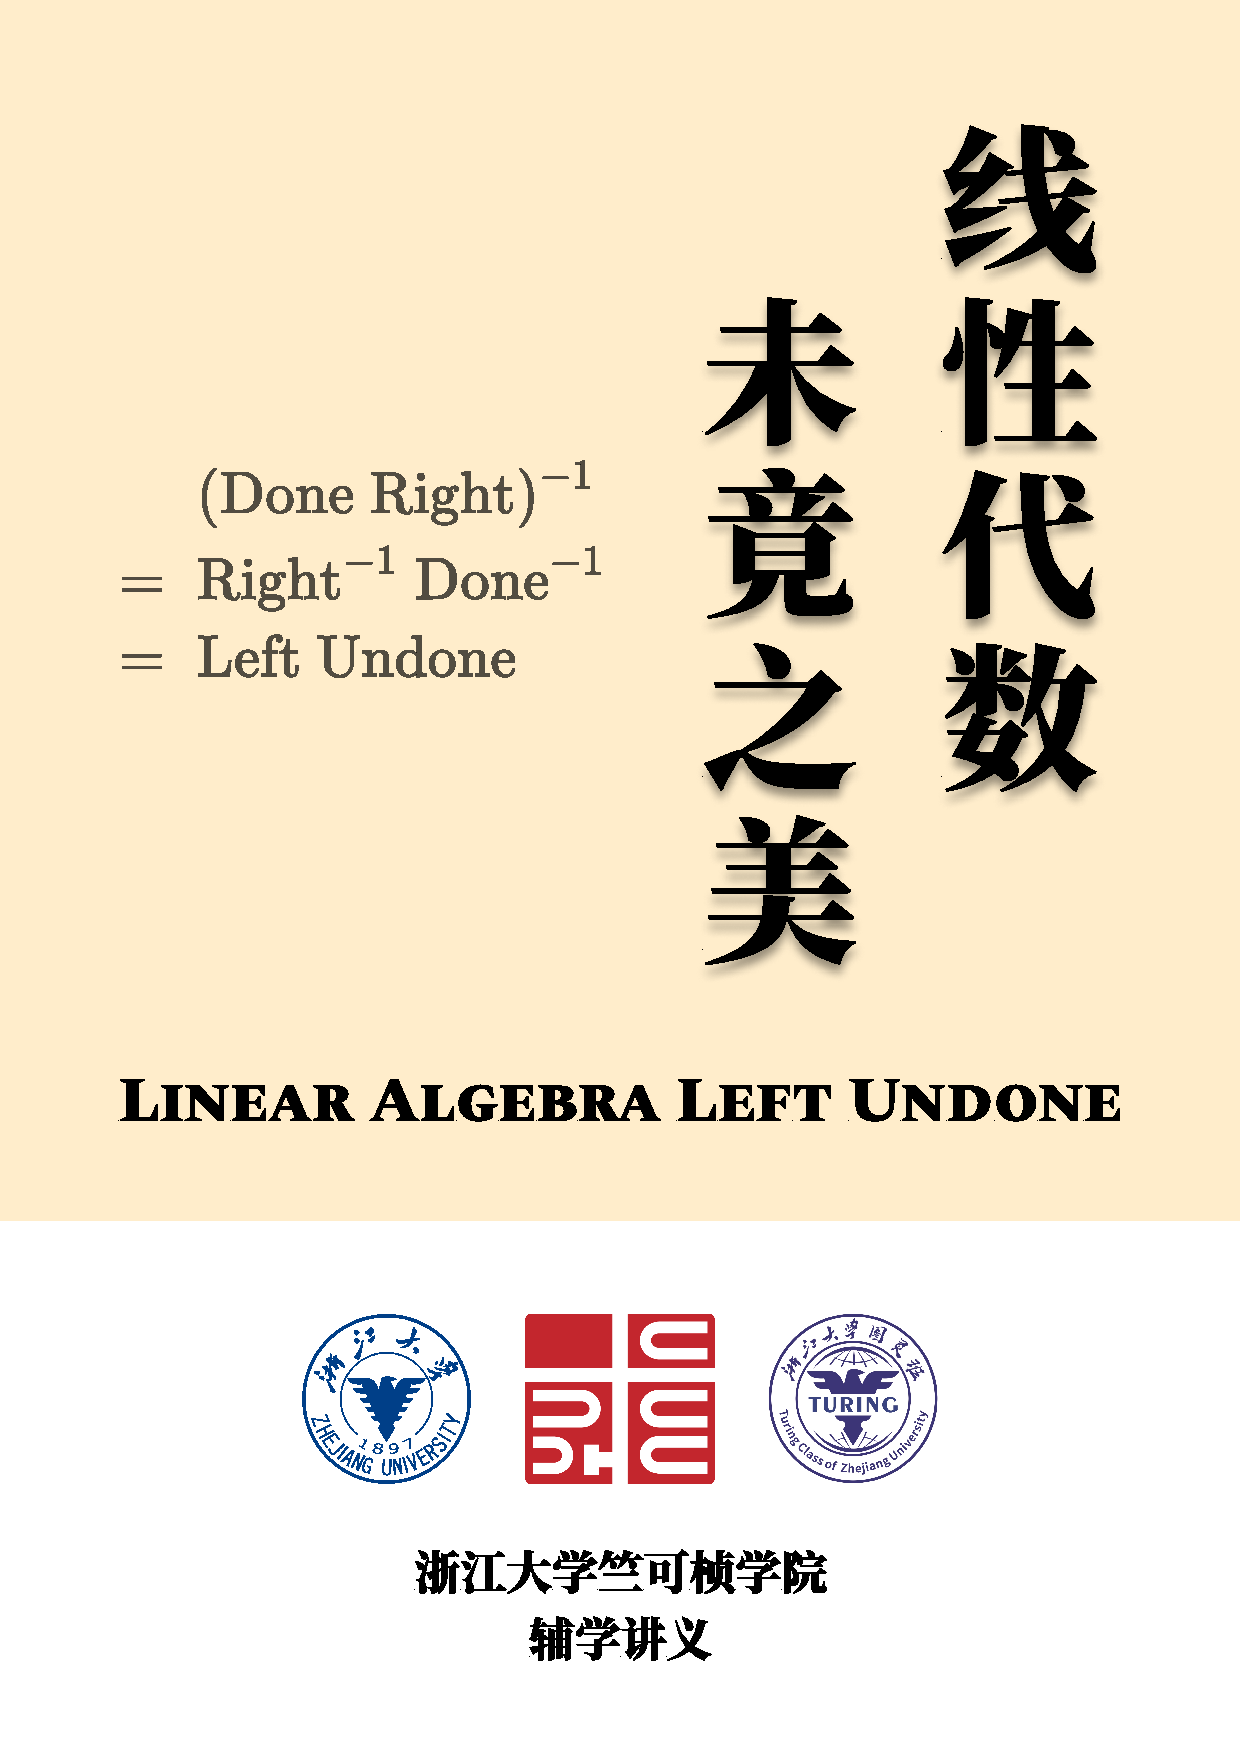
\includepdf[pages={1}]{./figs/cover.pdf}

\songti

% 插入空页
{\null
\thispagestyle{empty}
\newpage}
\setcounter{page}{1}

\pdfbookmark[0]{目录}{contents}
\tableofcontents

\addtolength{\parskip}{.5em}

\mainmatter
\setcounter{page}{1} % 将页码计数设置为 1
\chapter{预备知识}

线性代数作为大学的第一门数学课,预修要求并不高. 我们默认读者具有基本的高中数学知识,因此关于集合、映射以及向量的基本知识我们不在此赘述. 这一讲我们将从基本代数结构开始,以便后续线性空间的引入,然后我们将介绍本书中常见的概念——等价类和最常用的算法之一——高斯消元法.

\section{基本代数结构}

我们选择从基本代数结构谈起,因为在以往的实践中我们深切地体会到直接引入线性空间的跳跃. 因此我们希望从更具象的例子开始,首先引入``代数结构''这一基本概念,然后在下一节中自然地引出线性空间的定义.

我们首先考察一个简单的例子:实数集$\mathbf{R}$,它是一个集合. 在初中我们便知道,在$\mathbf{R}$上我们可以定义加法和乘法两种运算. 本质而言,运算是一种映射(或者更通俗而言,函数):

\begin{center}
    \begin{tabular}{rrcl}
        $+\enspace\colon$      & $\mathbf{R}\times\mathbf{R}$ & $\to$     & $\mathbf{R}$ \\
                               & $(a,b)$                      & $\mapsto$ & $a+b$        \\
        $\times\enspace\colon$ & $\mathbf{R}\times\mathbf{R}$ & $\to$     & $\mathbf{R}$ \\
                               & $(a,b)$                      & $\mapsto$ & $a\times b$
    \end{tabular}
\end{center}

上面的定义中出现了一个新的记号,即两个集合之间出现了乘号,这实际上是集合的笛卡尔积运算,定义如下:

\begin{definition}
    设$A$和$B$是两个非空集合,我们把集合
    \[A\times B=\{(a,b) \mid a\in A, b\in B\}\]
    称为集合$A$和$B$的\keyterm{笛卡尔积}[Cartesian product].
\end{definition}

因此我们很容易理解$\mathbf{R}\times\mathbf{R}$是一个集合,它的元素是形如$(a,b)$的有序对,其中$a,b\in\mathbf{R}$. 事实上,我们可以将$\mathbf{R}\times\mathbf{R}$看作平面上的点集,其中的点$(a,b)$对应于平面上的一个点,这一点的横坐标为$a$,纵坐标为$b$.

我们回到运算的映射表示,我们发现$+$和$\times$两个映射以两个实数作为函数的自变量,函数值也是一个实数. 或许读者看到这里还是对运算的定义有些许迷茫,但如果我们回忆映射的基本定义$f:A\to B$,$a\mapsto f(a)$,并将加法乘法写成$+(2,3)=5$,$\times(2,3)=6$,想必就会恍然大悟:$+$和$\times$实际上就是函数名,函数做的事情就是输入两个自变量然后进行加法/乘法运算得到函数值.

在上述讨论中,我们所做的事情很简单,就是给定一个集合,然后在这一集合的元素之间定义运算. 实际上这就是代数系统的定义:
\begin{definition}[{\keyterm{代数系统}[algebraic system]}]
    一般地,我们把一个非空集合$X$和在$X$上定义的若干代数运算$f_1,\ldots,f_k$组成的系统称为\keyterm*{代数系统}(简称代数系),记作$\langle X : f_1,\ldots,f_k\rangle$.
\end{definition}

特别注意的是,代数系统上定义的运算必须保证封闭性,也就是运算后的结果必须仍然在集合$X$中.

不难理解,代数系统其中蕴含的性质与其中定义的运算具有的性质是关联很大的. 我们仍然以实数域为例,介绍在代数学中关心的几个运算性质. 我们首先讨论实数域上的加法运算,以下性质对于任意$a,b,c\in\mathbf{R}$都成立:

\begin{enumerate}
    \item 结合律:$(a+b)+c=a+(b+c)$;

    \item 单位元:存在一个元素0,使得$a+0=0+a=a$;

    \item 逆元:对于任意$a$,存在一个元素$-a$,使得$a+(-a)=(-a)+a=0$(0为单位元);

    \item 交换律:$a+b=b+a$.
\end{enumerate}

对于乘法运算(可记为$\cdot$或$\times$),单位元一般记为1(更一般的可以记为$e$),逆元记为$a^{-1}$. 事实上,我们可以给出更多的例子:
\begin{example}\label{ex:1:Abel 群}
    \begin{enumerate}
        \item 代数系统$\langle \mathbf{R}\backslash\{0\}:\circ\rangle$定义的一般乘法运算

        \item 代数系统$\langle \mathbf{R}^2:+\rangle$定义的平面向量的加法
    \end{enumerate}
    均满足上述四条运算性质.
\end{example}

事实上,我们可以对上面的定义做进一步的抽象. 我们可以忽略集合中元素的差异(元素可以是实数,也可以是上述例子中的平面向量等),同时也可以忽略运算定义的差异,只关心运算作用于集合元素的性质. 对于一般的代数系统$\langle G:\circ\rangle$,我们有如下定义:
\begin{definition}[群] \label{def:1:群}
    若运算$\circ$满足结合律,则称代数系统$\langle G:\circ\rangle$为\keyterm{半群}[semigroup];若在半群基础上存在单位元,则称之为\keyterm{含幺半群}[monoid];若在含幺半群基础上每个元素存在逆元,则称之为\keyterm{群}[group];若在群的基础上运算还满足交换律,则称之为\keyterm{Abel群}[Abelian group],也称\keyterm{交换群}[commutative group].
\end{definition}

\autoref{def:1:群} 给出了我们本节第一个要讨论的代数结构——群的定义. 简而言之,代数结构就是在集合上定义具有某些特定性质的运算后得到的一类代数系统. 事实上,教材中42--44页给出了大量抽象的例子有助于同学们理解上述一系列群的定义,并且我们在后续学习矩阵的时候也会遇到一些群结构,相信这些实例能使读者体会到``在集合上定义运算''的方式的多样与抽象.

为方便书写,对于\autoref{def:1:群} 定义的群$\langle G:\circ\rangle$我们可以简写为群$G$. 除此之外,我们还需要指出以下两点:
\begin{theorem}\label{thm:1:群的单位元逆元唯一}
    \begin{enumerate}
        \item 群的单位元唯一;

        \item 群的每个元的逆元唯一.
    \end{enumerate}
\end{theorem}

\begin{proof}
    \begin{enumerate}
        \item 设$e_1$和$e_2$都是群$G$的单位元,则
              \[e_1=e_1\circ e_2=e_2.\]

        \item 设$b$和$c$都是$a$的逆元,则
              \[b=b\circ e=b\circ(a\circ c)=(b\circ a)\circ c=e\circ c=c.\]
    \end{enumerate}
\end{proof}

其中第一点的证明直接使用了单位元的性质,第二点的证明则使用了结合律和逆元的性质. 这里关于唯一性的证明是非常重要的:我们只需假设要证明唯一的东西有两个,然后说明这两个必然相等即可. 这一思想在之后证明矩阵的逆唯一等问题时也会用到,因此此处特别给出证明强调.

事实上,在很多集合上我们不仅可以定义一种运算,也可以定义两种甚至更多运算,在代数结构中我们仅讨论最多两种运算的情况. 事实上,我们最开始的实数集合定义加法和乘法的例子便可以引入一个新的代数结构——域:
\begin{definition}[{\keyterm{域}[field]}]
    我们称代数系统$\langle F:+,\circ\rangle$为一个\keyterm*{域},如果
    \begin{enumerate}
        \item $\langle F:+\rangle$是交换群,其单位元记作0;

        \item $\langle F\backslash\{0\}:\circ\rangle$是交换群;

        \item 运算$\circ$对$+$满足左、右分配律,即
              \begin{gather*}
                  a\circ(b+c)=a\circ b+a\circ c \\
                  (b+c)\circ a=b\circ a+c\circ a
              \end{gather*}
    \end{enumerate}
\end{definition}

显然,实数域$\mathbf{R}$上定义一般的实数加法和乘法后构成一个域. 实际上我们熟悉的例如有理数、实数等集合关于一般的加法和乘法运算都构成域,因此我们会经常使用``有理数域''、``实数域''等说法. 我们称数集对数的加法和乘法构成的域为数域,注意此处运算的定义必须是数学分析中定义的数的加法和乘法,不能是自定义的运算.
\begin{theorem}
    关于数域,我们有如下两个结论:
    \begin{enumerate}
        \item 数集$F$对数的加法和乘法构成数域的充要条件为:$F$包含0,1且对数的加、减、乘、除(除数不为0)运算封闭;

        \item 任何数域都包含有理数域$\mathbf{Q}$,即$\mathbf{Q}$是最小的数域.
    \end{enumerate}
\end{theorem}

上述定理的证明可见教材46页. 事实上,如果加法和乘法的定义不是数的加法和乘法,我们可以定义除了数域之外的域,我们将在本讲介绍完等价类的概念后给出这样的例子.

当然,还有一种代数结构对于$\circ$运算的要求有所降低,但也有广泛的应用,这就是环:
\begin{definition}[环]
    我们称代数系统$\langle R:+,\circ\rangle$为一个\keyterm{环}[ring],如果
    \begin{enumerate}
        \item $\langle R:+\rangle$是交换群,其单位元记作0;

        \item $\langle R:\circ\rangle$是半群;

        \item 运算$\circ$对$+$满足左、右分配律,即
              \begin{gather*}
                  a\circ(b+c)=a\circ b+a\circ c \\
                  (b+c)\circ a=b\circ a+c\circ a
              \end{gather*}
    \end{enumerate}

    若关于$\circ$存在单位元,则称之为\keyterm{含幺环}[ring with identity],若进一步每个非0($+$运算单位元)元素关于$\circ$都有逆元,则称之为\keyterm{除环}[division ring]. 另外,若上述定义中$\circ$运算满足交换律,则称为\keyterm{交换环}[commutative ring],结合上述除环和交换环两个定义,我们可以发现,交换除环即为域.
\end{definition}

\begin{example}
    利用定义验证下述关于代数系统的结论:
    \begin{enumerate}
        \item 整数集$\mathbf{Z}$对整数的加法和乘法构成一个交换环,但不是域;

        \item 设$C[a,b]$是闭区间$[a,b]$上的连续函数的集合;它对函数的加法和乘法构成一个环;

        \item 设$Q(\sqrt{2})=\{a+b\sqrt{2} \mid a,b\in\mathbf{Q}\}$,则$Q(\sqrt{2})$是一个数域.
    \end{enumerate}
\end{example}

我想大部分读者都会对抽象出代数结构的原因表示不解,如果这个问题无法解答,我想在下一章直接引入抽象的线性空间更会引发同学们对于``学了这个有什么用''的怀疑. 我们可以举一些不那么贴切但具象的例子来说明这其中的意义. 读者高中阶段想必大都经受过解析几何的摧残,大家在拿到题目时总会首先观察到题目属于``定点''、``定值''或是``极值''等问题,大家将自动与自己做题的经验或技巧匹配用于解答这几类问题. 同理,在研究一个特定的代数系统(例如定义了加法和乘法的实数域)的性质时,我们可以首先将其归类为群、环或是域等,然后我们只需要利用群环域各自的性质来研究这个代数系统的性质,而不需要再去研究这个代数系统的具体定义. 在这一过程中我们实现了问题的``归约'',即将一个复杂的问题转化为一个简单的更为抽象的问题,正如将解决上千道解析几何问题转化为研究几种题型的技巧. 这一``归约''的思想在将来的学习生活中我们将经常遇见,在实际中例如投资股票时我们可以将投资转化为提高投资组合的期望收益而尽力降低方差(风险)的求取极值的问题,在理论中,例如在计算理论的学习中我们会学习更为形式化的对问题的归约,这在算法复杂性研究中是基础的思想. 对于这类抽象问题感兴趣的同学不妨可以选择数学科学学院的抽象代数等课程,或是阅读本讲义的``后继''教程\href{https://frightenedfoxcn.github.io/notes/series/alg-for-cs/}{《写给计算机系学生的代数》}作进一步的了解. 事实上,对于理论感兴趣的同学,抽象代数将是必不可少的基础课程,它将是密码学、量子计算、计算理论以及编程语言理论等诸多领域的必要基础.

当然,这段描述因为涉及的知识容量较大,大概无法说服每一个读者. 但我们会在学习线性空间、线性映射的过程中不断重复这些思想,直到读者具备的知识容量足够时,一定能领会其中的奥妙.

\section{复数域的引入}

本书前半段讨论的框架是实数域、复数域都适用的,当然为了简化,我们的例子大都来源于实数. 从多项式一讲开始,我们便会开始强调实数域和复数域结论的不同,因此我们有必要在此引入复数域.

直观来看,实数位于数轴上,复数则分布在二维平面上,因此我们可以先考虑平面点集$\mathbf{R}^2$,并在其上定义加法和乘法运算使其成为一个域. 我们回顾高中学习的平面向量知识,我们记$\vec{e}_1=(1,0)$,$\vec{e}_2=(0,1)$,则$\mathbf{R}^2$上的任一向量$\vec{u}=(x,y)$可写为$x\vec{e}_1+y\vec{e}_2$. 此外,我们仍沿袭高中对向量长度的定义,即$\lvert\vec{u}\rvert=\sqrt{x^2+y^2}$.

在\autoref{ex:1:Abel 群} 中我们已经验证了$\mathbf{R}^2$上的向量加法满足Abel群的条件,因此我们只需要定义$\mathbf{R}^2$上的乘法使得代数系统$\langle\mathbf{R}^2\backslash\{(0,0)\}:\circ\rangle$也为Abel群. 这一乘法的构造需要满足一些自然的条件,同时也能实现构成Abel群的要求. 事实上,我们有如下定理:
\begin{theorem}\label{thm:1:复数乘法构造}
    平面点集$\mathbf{R}^2$上存在唯一的乘法$\circ$,满足
    \begin{enumerate}
        \item (单位元) $\vec{u}\circ\vec{e}_1=\vec{e}_1\circ\vec{u}=\vec{u},\enspace\forall\vec{u}\in\mathbf{R}^2$;

        \item (长度可乘性) $\lvert\vec{u}\circ\vec{v}\rvert=\lvert\vec{u}\rvert\lvert\vec{v}\rvert$.
    \end{enumerate}
    此乘法满足交换律,且使得$\langle\mathbf{R}^2:+,\circ\rangle$成为域.
\end{theorem}

上述定理中第一个条件是非常自然的,因为在二维平面上,$\{(x,0) \mid x\in\mathbf{R}\}$实际上就是实数轴,因此$\vec{e}_1=(1,0)$相当于实数1,因此作为乘法单位元是非常自然的. 第二条长度可乘则看起来没那么自然,但在接下来的证明中我们将会了解到其意义.

\begin{proof}
    对任意向量$\vec{u}=(a,b)=a\vec{e}_1+b\vec{e}_2,\enspace \vec{v}=(c,d)=c\vec{e}_1+d\vec{e}_2$,我们利用乘法的第一条性质有
    \[\vec{u}\circ\vec{v}=ac\vec{e}_1+(ad+bc)\vec{e}_2+bd\vec{e}_2\circ\vec{e}_2.\]
    由此可见$\vec{u}\circ\vec{v}=\vec{v}\circ\vec{u}$,因此乘法满足交换律. 同时可知,要定义乘法,关键是定义$\vec{e}_2\circ\vec{e}_2$的值.

    记$\vec{e}_2\circ\vec{e}_2=(x,y)$,由长度可乘性知$x^2+y^2=1$,另一方面
    \[(\vec{e}_1+\vec{e}_2)\circ(\vec{e}_1-\vec{e}_2)=\vec{e}_1-\vec{e}_2\circ\vec{e}_2=(1-x,y).\]
    由$|\vec{e}_1+\vec{e}_2|=|\vec{e}_1-\vec{e}_2|=\sqrt{2}$以及长度可乘性可得
    \[4=|(\vec{e}_1+\vec{e}_2)\circ(\vec{e}_1-\vec{e}_2)|^2=(1-x)^2+y^2.\]
    由此求出$x=-1,\enspace y=0$. 这说明
    \[\vec{e}_2\circ\vec{e}_2=-\vec{e}_1.\]
    由此得乘法的定义$\vec{u}\circ\vec{v}=(ac-bd)\vec{e}_1+(ad+bc)\vec{e}_2$,即
    \[(a,b)\circ(c,d)=(ac-bd,ad+bc).\]
    可验证,此乘法以$\vec{e}_1$为单位元,等式$(ac-bd)^2+(ad+bc)^2=(a^2+b^2)(c^2+d^2)$表明乘法满足长度可乘性. 上述证明亦表明乘法唯一(只能这么构造$\vec{e}_2\circ\vec{e}_2$).

    接下来我们很容易验证$\langle\mathbf{R}^2:+,\circ\rangle$满足域的定义,我们留作习题供读者自行验证.
\end{proof}

在\autoref{thm:1:复数乘法构造} 赋予的乘法下,$\langle\mathbf{R}^2:+,\circ\rangle$称为复数域$\mathbf{C}$. 我们自然地将$\vec{e}_1$合理简记为1,同时$\vec{e}_2$简记为$\i$,因为此时$(a,b)$即为$a+b\i$,并且利用$\vec{e}_2^2=-\vec{e}_1$可知$\i^2=-1$,这与我们熟知的虚数单位的定义是统一的. 这一代数表示引入的相关概念,如实部、虚部、纯虚数,以及复数四则运算法则在高中阶段大家都已熟知,在此不再赘述.

非零复数$z=x+y\i$也可写为极坐标的形式,即$z=|z|(\cos\theta+\i\sin\theta)$,其中$|z|=\sqrt{x^2+y^2}$为复数的平面表示的模长,$\theta\in\mathbf{R}$为连接原点与$z$的有向线段与$x$轴正方向的夹角(在相差$2\pi$整数倍的意义下唯一). 我们称$\theta$为复数$z$的辐角. 关于复数的模长我们有经典的三角不等式:
\begin{theorem}
    设$z,w\in\mathbf{C}$,则有$|z+w|\leqslant|z|+|w|$.
\end{theorem}

这一定理的几何意义是非常显然的,我们将$z$和$w$放在平面直角坐标系中观察就可以明白这就是经典三角不等式的复数版本. 等号成立的条件也显而易见,即$z$和$w$要么至少一个为0,要么都非零且$z$和$w$位于从原点出发的同一条射线上. 严格的证明如下:

\begin{proof}
    \begin{align*}
        |z+w|^2 & =(z+w)(\overline{z}+\overline{w})       \\
                & =|z|^2+|w|^2+2\Re(z\overline{w})        \\
                & \leqslant|z|^2+|w|^2+2|z||\overline{w}| \\
                & =(|z|+|w|)^2.
    \end{align*}
    等号成立当且仅当$z\overline{w}$为非负实数,与前述直观可得的的条件是等价的.
\end{proof}

证明中用到了一些应当熟知的结论,如$|z|^2=z\overline{z}$等,我们默认读者具有这些基础知识,因此不在此赘述.

\section{等价关系}

我们时常需要讨论集合中元素之间的关系. 例如直线间的平行、垂直、相交,或是数之间的大于、等于、小于关系.``关系''在我们的讲义中将会多次出现,因此我们很有必要在此形式化定义这一概念,并强调其中一类特定的关系——等价关系.

我们首先从(二元)关系这一概念入手. 实际上,这里的二元关系和日常生活中的关系是紧密相连的,例如将全人类作为谈论的背景集合,那么$(\text{小头爸爸}, \text{大头儿子})$这一有序二元组是符合这一关系的,但$(\text{章鱼哥}, \text{海绵宝宝})$显然不符合. 因此我们可以将父子关系看作笛卡尔积集合$\text{人类}\times\text{人类}$的子集. 更一般化的,集合$A$中的关系可以由$A\times A$的子集
\[\{(a,b) \mid a,b\in A, \enspace a\,R\,b\}\]
来刻画,其中$R$是这个关系本身(实质上是两个元素之间的某种性质),例如之前讨论的父子关系,或是数学中的大于、小于或同余等. 事实上,反过来,由$A\times A$的子集可以确定一个关系,例如我把全世界所有的父子组合放在这个集合中,那么这个集合就定义了人类中的父子关系.
\begin{example}
    以下是一些关系的例子:
    \begin{enumerate}
        \item 设$A=\mathbf{R}$,则$A\times A$的子集
              \[\{(a,b)\in A\times A \mid a^2+b^2=1\}\]
              定义了一个关系$R$,即
              \[a\,R\,b \iff a^2+b^2=1.\]

        \item 设$A=\{1,2,3\}$,则$A\times A$的子集
              \[\{(1,1),(1,2),(1,3),(2,2),(2,3),(3,3)\}\]
              定义了一个关系$R$,即
              \[a\,R\,b \iff a\leqslant b.\]

        \item 设$A$为任意数集,定义在$A$上的函数$f$也是一种关系,集合$A\times A$的子集
              \[B=\{(a,b)\in A\times A \mid b=f(a)\}\]
              刻画了这一关系. 换言之,函数是一种特殊的关系,它要求$\forall a\in A$有且仅有一个元素$b\in A$使得$(a,b)\in B$,其中$B$为上述定义的$A\times A$的子集.

        \item 设$A=\mathbf{Z}$,关系$R$满足$a\,R\,b\iff a\equiv b \pmod n$,即模$n$同余,则$A\times A$的子集
              \[\{(a,b)\in A\times A \mid a\equiv b \pmod n\}\]
              可以刻画这一关系.
    \end{enumerate}
\end{example}

接下来我们要讨论一种特别的关系,即等价关系. 它对关系$R$有一定的规定:
\begin{definition}\label{def:1:等价关系}
    集合$A$中关系若满足以下条件:
    \begin{itemize}
        \item (自反性) $\forall a\in A, \enspace a\,R\,a$;

        \item (对称性) 若$a\,R\,b$,则$b\,R\,a$;

        \item (传递性) 若$a\,R\,b$,$b\,R\,c$,则$a\,R\,c$,
    \end{itemize}
    则称$R$为$A$的一个等价关系. 进一步地,若$R$是集合$A$的一个等价关系且$a,b\in A$,若$a\,R\,b$,则称$a$,$b$关于$R$是等价的,并把$A$中所有与$a$等价的元素集合
    \[\overline{a}=\{b\in A \mid b\,R\,a\}\]
    称为$a$所在的等价类,$a$称为这个等价类的代表元素,并记$\{\overline{a}\}$为所有等价类为元素构成的集族.
\end{definition}

我们可能需要一个例子来理解这些概念. 我们不难证明,初等数论中的同余关系是一种等价关系,以模3同余为例,我们取整体集合为正整数集合,对于3,它的等价类就是所有和3模3同余的元素集合,即所有3的倍数. 同理,对于1,它所在的等价类就是模3余1的全体正整数,2所在的等价类是全体模3余2的正整数. 除此之外,我们还发现一个特点,即这三个等价类将原集合分成了三个无交集的子集
\begin{gather*}
    \overline{0}=\{3k\mid k\in\mathbf{Z}\} \\
    \overline{1}=\{3k+1\mid k\in\mathbf{Z}\} \\
    \overline{2}=\{3k+2\mid k\in\mathbf{Z}\}
\end{gather*}
且它们的并集就是原集合,即这三个等价类构成了原集合的一个\keyterm{分划}[partition](即分为并为原集合且互不相交的子集). 这一结论对所有等价类都成立,是很直观的结论:
\begin{theorem}\label{thm:1:等价类的性质}
    设$R$是集合$A$的等价关系,则由所有不同的等价类构成的子集族$\{\overline{a}\}$是$A$的分划. 反之,我们也可以基于分划在$A$中定义等价关系.
\end{theorem}

证明这一定理需要一个引理:
\begin{lemma}
    设$R$是集合$A$的等价关系,$a,b\in A$,则$\overline{a}=\overline{b}\iff a\,R\,b$.
\end{lemma}
这一引理说明$a$和$b$等价当且仅当它们等价类相同,或者说在同一个等价类中,相信根据等价类的定义这是很显然的结论.

这一引理还有一个重要的推论:
\begin{corollary}\label{cor:1:等价类的性质}
    设$R$是集合$A$的等价关系,$a,b\in A$,则下面二者必成立其一:
    \begin{enumerate}
        \item $\overline{a}\cap\overline{b}=\varnothing$;
        \item $\overline{a}=\overline{b}$.
    \end{enumerate}
\end{corollary}
即等价类要么相等要么不相交,这一结论也是非常自然的,且由这一结论我们很容易证明\autoref{thm:1:等价类的性质}. 如果对这些定理的证明细节感兴趣的读者可以参看教材第5页的定理1.1和1.2.

进一步此我们可以定义商集的概念:
\begin{definition}[{\keyterm{商集}[quotient set]}]
    设$R$是集合$A$的等价关系,以关于$R$的等价类为元素的集合(实际上是集合构成的集合,又称集族)$\{\overline{a}\}$称为$A$对$R$的\keyterm*{商集},记为$A/R$. 由
    \[\pi(a) = \overline{a}, \enspace \forall a\in A\]
    定义的$A$到$A/R$上的映射$\pi$称为$A$到$A/R$上的自然映射.
\end{definition}
我们可以看到,自然映射$\pi$将$A$中的元素$a$映到自己所在的等价类$\overline{a}$. 基于上述定义,我们可以完成在基本代数结构一节中遗留的一个问题:我们能否定义非数域的域?答案是肯定的,如果同学们对密码学感兴趣的应当听闻过有限域这一概念,接下来我们将通过简单的例子来说明这一概念.

\begin{example}\label{ex:1:有限域}
    设$Z_n$是$\mathbf{Z}$关于模$n$同余关系$R$的商集,即
    \[Z_n=\mathbf{Z}/R=\{\overline{0},\overline{1},\ldots,\overline{n-1}\}.\]
    即$Z_n$中的元素是$n$个集合,其中第$i$个集合是全体模$n$余$i-1\enspace(i=1,2,\ldots,n)$的整数构成的集合.

    在$Z_n$上定义加法$\oplus$为$\overline{a}\oplus\overline{b}=\overline{a+b}$. 这里$a$和$b$并不一定要在$0$到$n-1$之间,因为事实上$\overline{a}=\overline{kn+a}\enspace(k\in\mathbf{Z})$. 我们只需对$a$,$b$以及$a+b$对$n$取模就可以将它们控制在$0$到$n-1$之间且表示的是同一个运算表达式(因为本质上只是我们选取了同一个等价类的不同代表元素进行计算,例如$n=3$时,$\overline{1}+\overline{2}=\overline{4}+\overline{8}=\overline{0}$).

    接下来我们需要定义乘法$\circ$,同样是一个自然的定义,即$\overline{a}\circ\overline{b}=\overline{ab}$. 我们很容易验证$\forall n\in\mathbf{Z}$且$n\geqslant 2$,$\langle Z_n:\oplus,\circ\rangle$构成一个含幺交换环. 教材43页例8和45页例3中有详细的证明,因为较为显然此处从略. 我们要讨论的是何时$\langle Z_n:\oplus,\circ\rangle$构成域,由此我们便构造了一个非数域的域,并且元素个数是有限的.

    我们这里可以给出结论:$\langle Z_n:\oplus,\circ\rangle$是域当且仅当$n$是素数. 这一结论的证明需要一些数论的知识,我们放在习题中供感兴趣的同学证明.
\end{example}

\section{高斯消元法}

高斯消元法是线性代数中最常用的算法之一,是之后解决大量问题所需要掌握的基本方法,同时也是考试中一定会考察的内容,无论是单独一个大题考察,还是嵌入在其它问题中. 教材中相关概念和算法的介绍已经非常详细,这里只作总结.

注意考试中单独考察解方程时,时间充足时建议将过程写完整,标明初等行变换的具体步骤,并且至少写出阶梯矩阵和行简化阶梯矩阵. 除此之外,需要保证计算中尽量减少错误,时间充足可以解完方程后将答案代入进行检查.

需要强调的是,不要认为本节内容很简单就放过了,实际上如果长期不计算高斯消元法很容易陷入眼高手低的窘境,因此希望各位同学熟悉高斯消元法的基本步骤并熟练应用.

一般的,对于一个由$m$个方程组成的$n$元(即变量数为$n$)线性方程组
\[ \begin{cases} \begin{aligned}
            a_{11}x_1+a_{12}x_2+\cdots+a_{1n}x_n & = b_1           \\
            a_{21}x_1+a_{22}x_2+\cdots+a_{2n}x_n & = b_2           \\
                                                 & \vdotswithin{=} \\
            a_{m1}x_1+a_{m2}x_2+\cdots+a_{mn}x_n & = b_m
        \end{aligned} \end{cases} \]
将其系数排列成矩阵
\[\begin{pmatrix}
        a_{11} & a_{12} & \cdots & a_{1n} \\
        a_{21} & a_{22} & \cdots & a_{2n} \\
        \vdots & \vdots & \ddots & \vdots \\
        a_{m1} & a_{m2} & \cdots & a_{mn}
    \end{pmatrix}\]
且记$\vec{b}=(b_1,b_2,\ldots,b_m)^\mathrm{T}$,若$\vec{b}=\vec{0}$则称此方程为齐次线性方程组,否则为非齐次线性方程组. 再将$n$个未知量记为$n$元列向量$X=(x_1,x_2,\ldots,x_n)^\mathrm{T}$,我们便可以把方程组简记为$AX=\vec{b}$.

令$\vec{\beta}_i=(a_{1i},a_{2i},\ldots,a_{mi})^\mathrm{T}$,即方程组系数矩阵的某一列,则方程组还可以记为$x_1\vec{\beta}_1+x_2\vec{\beta}_2+\cdots+x_n\vec{\beta}_n=\vec{b}$,这一形式将在之后多次见到.

在以上的记号下,我们可以将解线性方程组的过程转化为矩阵的初等行变换. 高斯消元法的一般步骤如下:
\begin{center}
    线性方程组$\overset{1}{\longrightarrow}$增广矩阵$\overset{2}{\longrightarrow}$阶梯矩阵$\overset{3}{\longrightarrow}$(行)简化阶梯矩阵$\overset{4}{\longrightarrow}$解
\end{center}

\begin{enumerate}[label=步骤\arabic*~]
    \item 只需要将线性方程组转化为$(A, \vec{b})$的形式,得到左$n$列为系数矩阵,最右列为列向量$\vec{b}$的$n+1$列的增广矩阵;

    \item 通过初等行变换后,得到教材P34(1--13)的形式的矩阵——阶梯矩阵. 阶梯矩阵系数全零行在最下方,并且非零行中,在下方的行的第一个非零元素一定在上方行的右侧(每行第一个非零元素称主元素);

    \item 将主元素化1后将主元素所在列的其他元素均通过初等行变换化为0即可;

    \item \label{item:1:解方程组}
          我们分三种情况讨论:
          \begin{enumerate}
              \item 有唯一解:没有全零行,最后一个主元素的行号与系数矩阵的列数相等,且行简化阶梯矩阵对角线上全为1,其余元素均为0,此时可以直接写出解;

              \item 无解:出现矛盾方程,即系数为0的行的行末元素不为0,此时直接写无解即可;

              \item 有无穷解:非上述情况. 此时设出自由未知量将其令为$k_1,k_2,\ldots$,然后代入增广矩阵对应的方程组即可. 注意选取自由未知量时,选取没有主元素出现的列对应的未知量会与标准答案更贴近(如教材P33选取$x_2,x_5$),当然选择其他作为自由未知量也可以.
          \end{enumerate}
\end{enumerate}

从高斯消元法开始,我们正式进入线性代数的学习. 实际上,上述 \ref*{item:1:解方程组} 中关于方程组解的情况的讨论我们是浮于表面,是基于算法最后得到的矩阵的形式进行的讨论,但事实上,这背后蕴含着更深刻的意义. 我们将会在接下来的十余个章节中讲述线性代数中的核心概念,并在\hyperref[chap:朝花夕拾]{朝花夕拾}中回过头来重新审视线性方程组解的问题. 相信在那时,经历十余章各式抽象概念和运算技巧的洗礼后再来回味这一问题的你,定有``守得云开见月明''之感,对线性代数的理解也会更深一层.

\vspace{2ex}
\centerline{\heiti \Large 内容总结}

本讲为了后续章节讲述方便引入了一些基本概念和算法. 尽管这是一门面向理工科应用的数学课,但我们仍然希望以最自然的方式引入概念,而非填鸭式地轰炸,因此我们首先从大家最熟悉的实数集合开始,讨论在集合上定义运算的方法:我们逐步加强条件,引入了三种基本的代数结构——群、环和域,并且给出了一些例子,并简单讨论了定义代数系统的意义. 事实上,下一讲开始要介绍的线性空间也是一种特殊的代数结构,因此首先引入代数结构对于我们自然展开接下来的讨论有很大的帮助,不至于让读者觉得非常突兀.

接下来我们也从域的定义入手,构造了$\mathbf{R}^2$上的乘法运算使其构成了一个域,并且我们发现这里的定义与高中学习的复数乘法是完全一致的. 之后我们引入了等价关系的概念,这一概念在后续的讲义中将会多次出现,其重要意义就是将一个集合划分成了几个等价的区域. 最后我们讨论了高斯消元法的一般步骤,这是我们接下来解决线性空间中各类问题绕不开的算法.

\vspace{2ex}
\centerline{\heiti \Large 习题}

\vspace{2ex}
{\kaishu 我这门课很简单,只有简单的加减乘除四则运算,甚至除法都不太需要.}
\begin{flushright}
    \kaishu
    ——浙江大学数学科学学院教授吴志祥
\end{flushright}

\centerline{\heiti A组}
\begin{enumerate}
    \item 完善\autoref{thm:1:复数乘法构造} 中的证明,即证明$\mathbf{R}^2$在平面向量加法和如\autoref*{thm:1:复数乘法构造} 定义的乘法下构成一个域.

    \item 完成教材48页第13题.

    \item 求齐次线性方程组$\begin{cases}
                  x_1+x_2+x_3+4x_4-3x_5=0   \\
                  2x_1+x_2+3x_3+5x_4-5x_5=0 \\
                  x_1-x_2+3x_3-2x_4-x_5=0   \\
                  3x_1+x_2+5x_3+6x_4-7x_5=0
              \end{cases}$的通解.

    \item 求非齐次线性方程组$\begin{cases}
                  x_1-x_2+2x_3-2x_4+3x_5=1     \\
                  2x_1-x_2+5x_3-9x_4+8x_5=-1   \\
                  3x_1-2x_2+7x_3-11x_4+11x_5=0 \\
                  x_1-x_2+-x_3-x_4+3x_5=3
              \end{cases}$的通解.

    \item 求解线性方程组$\begin{cases}
                  x_1+x_2+x_3=1   \\
                  x_1+2x_2-5x_3=2 \\
                  2x_1+3x_2-4x_3=5
              \end{cases}$.
\end{enumerate}

\centerline{\heiti B组}
\begin{enumerate}
    \item 设$A$是一个Abel群,$A$的运算是加法. 在$A$中定义乘法运算为$ab=0,\enspace\forall a,b\in A$. 证明:$A$为一个环(我们称这种环为\keyterm*{零环}[zero ring]).

    \item 证明:若集合$A$上的二元关系$R$满足
          \begin{enumerate}
              \item $a\,R\,a,\enspace\forall a\in A$;

              \item $\forall a,b,c\in A$,若$a\,R\,b$且$a\,R\,c$,则$b\,R\,c$.
          \end{enumerate}
          则$R$为$A$上的等价关系.
\end{enumerate}

\centerline{\heiti C组}
\begin{enumerate}
    \item 证明:\autoref{ex:1:有限域} 中定义的$\langle Z_n:\oplus,\circ\rangle$是域当且仅当$n$是素数.
          (提示:无论$n$是否为素数,$n\in\mathbf{Z}$且$n\geqslant 2$时$\langle Z_n:\oplus,\circ\rangle$为含幺交换环,因此是否为素数将决定这一结构中每个元素是否有逆元. 在初等数论中,我们熟知的裴蜀定理可以解决这一问题.)

    \item 本讲我们构造了$\mathbf{R}^2$上的乘法,从而定义了复数域的乘法运算. 本题希望探讨的是:$\mathbf{R}^3$无法构造出乘法使其成为一个域. 在高中的学习中我们知道,$\mathbf{R}^3$空间向量的一组基底为$\{\vec{e}_1=(1,0,0),\vec{e}_2=(0,1,0),\vec{e}_3=(0,0,1)\}$. 证明:$\mathbf{R}^3$没有乘法同时满足以下性质:
          \begin{enumerate}
              \item (单位元) $\forall \vec{u}\in\mathbf{R}^3,\enspace\vec{e}_1\cdot \vec{u}=\vec{u}\cdot \vec{e}_1$;

              \item (交换性) $\forall \vec{u},\vec{v}\in\mathbf{R}^3,\enspace\vec{u}\cdot \vec{v}=\vec{v}\cdot \vec{u}$;

              \item (长度可乘性) $\forall \vec{u},\vec{v}\in\mathbf{R}^3,\enspace|\vec{u}\cdot\vec{v}|=|\vec{u}||\vec{v}|$.
          \end{enumerate}
          按照如下思路给出详细证明过程:采用反证法. 假设乘法存在,则
          \begin{enumerate}
              \item 通过计算$(\vec{e}_1+\vec{e}_2)\cdot(\vec{e}_1-\vec{e}_2)$,$(\vec{e}_1+\vec{e}_3)\cdot(\vec{e}_1-\vec{e}_3)$,证明\[\vec{e}_2\cdot\vec{e}_2=\vec{e}_3\cdot\vec{e}_3=-\vec{e}_1.\]

              \item 证明$(\vec{e}_2+\vec{e}_3)\cdot(\vec{e}_2-\vec{e}_3)=0$得出矛盾.
          \end{enumerate}
\end{enumerate}

\chapter{线性空间}

本讲我们将开始回答第 1 讲最后留下的问题,即线性方程组有唯一解、无穷解或无解的本质原因. 这段旅程或许有些漫长,中间会有很多的铺垫,我们将从其中最为基础的概念——线性空间出发进行探讨.

回忆高斯消元法,方程组中每一行或一列都可以视为向量. 我们可以先看下面这个例子:
\begin{example}\label{ex:2:线性空间引入}
    考虑如下两个方程组
    \begin{multicols}{2}
        \item $\begin{cases}
                x_1+x_2+x_3=0   \\
                x_1+2x_2+3x_3=0 \\
                2x_1+3x_2+4x_3=0
            \end{cases}$

        \item $\begin{cases}
                x_1+x_2+x_3=0   \\
                x_1+2x_2+3x_3=0 \\
                x_1+3x_2+4x_3=0
            \end{cases}$
    \end{multicols}
    不难解得,第一个方程组有无穷解,第二个方程组有唯一解. 从高斯消元法的过程来看,第一个方程组的简化阶梯矩阵出现了全零行,其原因是显而易见的:因为方程组第一行和第二行相加正好是第三行,因此可以直接消去第三行,即三行的系数矩阵的三个行向量
    \[\alpha_1=(1,1,1),\enspace\alpha_2=(1,2,3),\enspace\alpha_3=(2,3,4)\]
    满足$\alpha_1+\alpha_2=\alpha_3$. 而第二个方程组系数矩阵行向量间没有类似的可互相消去的关系.
\end{example}

从上面这一例子中我们可以看出,方程组的解与系数矩阵的行向量之间的关系密切相关. 因此我们会有一个很自然的想法,即我们需要研究向量之间的关联. 受第1讲基本代数结构的启发,我们应当自然地想到我们需要引入一个代数结构,从而使得我们可以统一地研究向量间的关联,这一代数结构便是线性空间.

\section{线性空间的定义}

\term{线性空间}\index{xianxingkongjian@线性空间 (linear space)}是我们接触的第一个核心概念,作为一种代数结构,它需要在非空集合$V$上定义运算. 其中第一个运算是我们熟知的加法$+$. 在线性空间的定义中,我们要求$\langle V:+\rangle$构成Abel群,即其中元素满足如下运算律:
\begin{enumerate}
    \item (结合律) $\alpha+(\beta+\gamma)=(\alpha+\beta)+\gamma,\enspace\forall \alpha,\beta,\gamma \in V$;

    \item (加法单位元) $\exists 0 \in V$使得$\forall\alpha\in V$ 有 $\alpha+0=0+\alpha$;

    \item (逆元) $\forall\alpha\in V,\enspace \exists \beta \in V$,有$\alpha+\beta=\beta+\alpha=0$,记$\beta=-\alpha$;

    \item (交换律) $\forall\alpha, \beta\in V,\enspace \alpha+\beta=\beta+\alpha$.
\end{enumerate}

第二种运算和之前学习的其他代数结构不同,我们需要首先引入一个数域$\mathbf{F}$,接下来在$\mathbf{F}\times V$上定义取值于$V$的数乘运算,即$\mathbf{F}\times V$中的每个元素$(\lambda,\alpha)\mapsto \lambda\alpha\in V$,并且数乘运算满足以下性质:$\forall \alpha,\beta \in V,\enspace\forall \lambda,\mu\in\mathbf{F}$以及$\mathbf{F}$上的乘法单位元1,有
\begin{enumerate}
    \item $1\cdot \alpha=\alpha$;

    \item $\lambda(\mu\alpha)=(\lambda\mu)\alpha$;

    \item $(\lambda+\mu)\alpha=\lambda\alpha+\mu\alpha$;

    \item $\lambda(\alpha+\beta)=\lambda\alpha+\lambda\beta$.
\end{enumerate}

基于此,我们完整定义了一个线性空间,我们一般称集合$V$关于上述两种运算在域$\mathbf{F}$上构成一个线性空间,简称为$V$在域$\mathbf{F}$上的线性空间,记作$V(\mathbf{F})$. 如果$\mathbf{F}$是实(复)数域,则称$V$为实(复)数域上的线性空间. 关于线性空间的定义,我们还有如下说明:
\begin{enumerate}
    \item 线性空间还有一个重要的概念是运算封闭,即线性空间中的元素进行加法或数乘运算后,得到的元素仍然是属于线性空间的. 这一点是定义要求的,加法封闭是 Abel 群的要求,因为 Abel 群要求加法运算定义为映射 $V\times V\to V$,因此$V$中两个元素相加后必须仍在$V$中(事实上这是代数系统的共性),数乘注意前述定义中数乘运算``取值于$V$''的要求,即它是 $F\times V\to V$ 的映射;

    \item 特别注意线性空间定义在非空集合上,事实上根据加法构成Abel群的要求,最小的线性空间也必须至少包含加法单位元(可以记为$V=\{0\}$).

    \item 结合我们上一讲对公理化的研究,事实上我们到目前为止也只定义了上面的加法、数乘运算和几条规则,我们需要忘记其他任何规则,由此出发进行推导出一些看似显然但公理没有直接给出的重要运算性质:
          \begin{enumerate}
              \item 由于加法运算构成Abel群,因此加法零元和逆元是唯一的,并且我们可以定义减法运算为加上一个元素的逆,即$\alpha-\beta=\alpha+(-\beta)$;

              \item 事实上,根据公理中的性质,我们可以逐步得到$\lambda(\alpha-\beta)+\lambda\beta=\lambda((\alpha-\beta)+\beta)=\lambda((\alpha+(-\beta))+\beta)=\lambda(\alpha+((-\beta)+\beta))=\lambda(\alpha+\vec{0})=\lambda\alpha$,两边分别加$-(\lambda\beta)$即可以得到
                    \begin{equation}\label{eq:2:线性空间运算性质1}
                        \lambda(\alpha-\beta)=\lambda\alpha-\lambda\beta.
                    \end{equation}
                    上面推导过程中第一个等号来源于数乘分配律,第二个等号来源于减法的定义(加上逆元),第三个等号来源于加法结合律,第四个等号来源于逆元的定义(加起来等于向量加法零元$\vec{0}$),最后一个等号来源于加法单位元的定义. 事实上这一过程是非常清晰的. 需要注意的一点是,接下来为了区分$V$中的零元和数域中的数0,我们将$V$中零元加粗,请读者务必仔细区分.

                    除此之外,$(\lambda-\mu)\alpha+\mu\alpha=(\lambda-\mu+\mu)\alpha=\lambda\alpha$,两边分别加$-(\mu\alpha)$即可以得到
                    \begin{equation}\label{eq:2:线性空间运算性质2}
                        (\lambda-\mu)\alpha=\lambda\alpha-\mu\alpha.
                    \end{equation}
                    事实上,\autoref{eq:2:线性空间运算性质1} 和\autoref{eq:2:线性空间运算性质2} 可以视为数乘运算对减法也满足分配律(但我们必须时刻牢记在心,数的减法是常规的,向量的减法是加上向量的逆元).

              \item 在\autoref{eq:2:线性空间运算性质1} 中分别令$\alpha=\beta$和$\alpha=\vec{0}$,在\autoref{eq:2:线性空间运算性质2} 分别令$\lambda=\mu$和$\lambda=0$有如下四条性质:
                    \begin{enumerate}
                        \item $\lambda\cdot \vec{0}=\vec{0}$;

                        \item $\lambda(-\beta)=-(\lambda\beta)$;

                        \item $0\cdot \alpha=\vec{0}$;

                        \item $(-\mu)\alpha=-(\mu\alpha)$.
                    \end{enumerate}
                    我们详细证明前两条如何根据公理一步步推导得到,后两条请读者依照此自行证明.
                    \begin{proof}
                        \begin{enumerate}
                            \item 在\autoref{eq:2:线性空间运算性质1} 中令$\alpha=\beta$,则$\lambda(\alpha-\alpha)=\lambda\alpha-\lambda\alpha$,根据减法定义有$\alpha-\alpha=\alpha+(-\alpha)=\vec{0}$,且$\lambda\alpha-\lambda\alpha=\lambda\alpha+(-(\lambda\alpha))=\vec{0}$,因此$\lambda\cdot \vec{0}=\vec{0}$.

                            \item 在\autoref{eq:2:线性空间运算性质1} 中令$\alpha=\vec{0}$有$\lambda(\vec{0}-\beta)=\lambda\vec{0}-\lambda\beta$,根据减法定义有$\vec{0}-\beta=\vec{0}+(-\beta)=-\beta$(第二个等号来源于加法单位元性质),且$\lambda\vec{0}-\lambda\beta=\vec{0}-\lambda\beta=\vec{0}+(-(\lambda\beta))=-(\lambda\beta)$(第一个等号来源于刚刚证明的$\lambda\cdot \vec{0}=\vec{0}$,第二个等号来源于减法的定义,第三个等号来源于加法单位元性质),因此$\lambda(-\beta)=-(\lambda\beta)$.
                        \end{enumerate}
                    \end{proof}
                    特别地,当$\mu=1$时有$(-1)\alpha=-\alpha$. 即$-1$数乘一个元素可以得到该元素的逆元(虽然代入一般平面向量这一点非常显然,但是我们只能基于公理一步步推导得到这一显然的性质).

              \item 若$\lambda\alpha=\vec{0}$,则$\lambda=0$或$\alpha=\vec{0}$,这一点也是显然的,因为如果$\lambda\neq 0$,则$\lambda^{-1}$存在,从而$\alpha=1\alpha=(\lambda^{-1}\lambda)\alpha=\lambda^{-1}(\lambda\alpha)=\lambda^{-1}\vec{0}=\vec{0}$(这里的每一个等号都是能找到对应的,请读者自行判断).

                    最后,综合上述性质我们有方程$\lambda\beta+\lambda_1\alpha_1+\lambda_2\alpha_2+\cdots+\lambda_r\alpha_r=\vec{0}$在$\lambda\neq 0$时的解为$\beta=-\lambda^{-1}\lambda_1\alpha_1-\lambda^{-1}\lambda_2\alpha_2-\cdots-\lambda^{-1}\lambda_r\alpha_r$. 我们放在习题中供读者练习.
          \end{enumerate}
\end{enumerate}

或许同学们会疑惑为什么线性空间会要求上述这8条性质(加法、数乘各4条). 事实上,这里的加法交换律是可以被其他7条推出的,感兴趣的同学可以自行尝试证明. 其余的7条公理彼此独立,每一条均不可取消. 感兴趣的同学可以试试举出反例来说明其余7条中每一条均不能由其余各条推出.

我们发现线性空间中定义的运算规则与我们高中学习的平面向量的加法和数乘是非常类似的,我们回顾未竟专题一关于公理化的讨论,实际上这就可以视为从简单的向量加法和数乘抽象出来的一些规则. 而公理的诞生应当是要尽可能简洁,而且有足够的表达力——这一点我们将来基于这一定义不断推出线性空间的性质时就会发现非常足够(事实上你现在就能通过我们上面证明的运算性质初步感知到这一点,因为7条公理中任何一条的缺失都会使得上面某条显然而合理的性质不再满足,而我们未来需要的性质都可以由此导出),因此皮亚诺在1888年正式给出这一定义并沿用至今. 但我们需要知道他的工作也是基于前人(如格拉斯曼)的工作不断修正而来的,只是我们被动接受这一概念使得这一自然的过程变得很突兀. 当然这门课只要求你记忆这8条性质,并请务必牢记于心,考试可能要求你验证线性空间. 记忆难度也并不大,Abel 群4条性质都有名称标注,数乘运算也是易于记忆的结合律和分配律加单位元性质.

除此之外,公理化定义还有一个很重要的作用就是使得我们可以不仅仅在向量集合的背景下定义线性空间,这使得我们可以将对于很多结构的研究都转化为对于线性空间的研究. 接下来我们给出一些与向量无关的线性空间的例子:

\begin{example}
    几种非常常见的线性空间,希望读者能熟知其性质:
    \begin{enumerate}
        \item (多项式)$\mathbf{F}[x]_{n+1}=\{a_0+a_1x+\cdots+a_nx^n \mid a_i\in\mathbf{F}\}$关于多项式的加法和数乘构成线性空间,但
              \[\mathbf{F}[x]'_{n+1}=\{a_0+a_1x+\cdots+a_nx^n \mid a_i\in\mathbf{F}, a_n\neq 0\}\]
              不构成线性空间.

              注:书上常将多项式记为$\mathbf{F}[x]_{n+1}$,表示次数不超过$n$的多项式的集合,而《线性代数应该这样学》中使用 $\mathcal{P}_n(\mathbf{F})$ 表示相同的集合.

              注意常见记号:$(k_1p_1+k_2p_2)(x)=k_1p_1(x)+k_2p_2(x)$.

        \item (复数与实数)可以验证:复数集$\mathbf{C}$是数域$\mathbf{C}$或数域$\mathbf{R}$上的线性空间. 此处一定注意复数集$\mathbf{C}$在此处同时出现在集合和数域中.

              注意:这一例子表明,同一集合可以在不同数域上构成不同的线性空间,在下一讲接触维数的定义后,我们也将知道二者的维数是不一样的(见\autoref{ex:3:不同数域的维数}).

              当然,不同的集合也可以在同一个数域上构成不同的线性空间,例如$\mathbf{C(R)}$和$\mathbf{R(R)}$.

        \item 对$n$维实非零系数向量空间$V$定义如下加法运算
              \begin{gather*}
                  \alpha = (a_1, a_2, \ldots, a_n), \beta = (b_1, b_2, \ldots, b_n) \in V = \mathbf{R}_{+}^n, \\
                  \alpha \oplus \beta = (a_1b_1, a_2b_2, \ldots, a_nb_n).
              \end{gather*}
              定义如下数乘运算
              \[\forall \lambda \in \mathbf{R}, \lambda \circ \alpha = (a_1^\lambda, a_2^\lambda, \ldots, a_n^\lambda).\]
              则$V$构成线性空间.

        \item $V=\{f \mid x \in \mathbf{R}, f(x) \in \mathbf{C}$(即$f$是实变量复值函数),且$f(-x)=\overline{f(x)}$(后者为$f(x)$的共轭复数)$\}$,定义如下的加法和数乘运算:
              \begin{gather*}
                  (f \oplus g)(x) = f(x) + g(x) \\
                  (\lambda \circ f)(x) = \lambda f(x).
              \end{gather*}
              则$V$构成线性空间.
    \end{enumerate}
\end{example}

\begin{solution}
    \begin{enumerate}
        \item 我们对八条性质进行逐条验证即可.
              \begin{enumerate}
                  \item $\forall p_1(x), p_2(x), p_3(x) \in \mathbf{F}[x]_{n+1}=\{a_0+a_1x+\cdots+a_nx^n \mid a_i\in\mathbf{F}\}$,有
                        \begin{align*}
                                & (p_1(x) + p_2(x)) + p_3(x)                                                                                \\
                            ={} & ((a_{10} + a_{11}x + \cdots  + a_{1n}x^n) + (a_{20} + a_{21}x + \cdots  + a_{2n}x^n))                     \\
                            +{} & (a_{30} + a_{31}x + \cdots  + a_{3n}x^n)                                                                  \\
                            ={} & ((a_{10} + a_{20}) + (a_{11} + a_{21}) x + \cdots  + (a_{1n} + a_{2n}) x^n)                               \\
                            +{} & (a_{30} + a_{31}x + \cdots  + a_{3n}x^n)                                                                  \\
                            ={} & (((a_{10} + a_{20}) + a_{30}) + ((a_{11} + a_{21}) + a_{31})x + \cdots + ((a_{1n} + a_{2n}) + a_{3n})x^n) \\
                            ={} & ((a_{10} + (a_{20} + a_{30})) + (a_{11} + (a_{21} + a_{31}))x + \cdots + (a_{1n} + (a_{2n} + a_{3n}))x^n) \\
                            ={} & (a_{10} + a_{11}x + \cdots  + a_{1n}x^n)                                                                  \\
                            +{} & ((a_{20} + a_{21}x + \cdots  + a_{2n}x^n) + (a_{30} + a_{31}x + \cdots  + a_{3n}x^n))                     \\
                            ={} & p_1(x) + (p_2(x) + p_3(x))
                        \end{align*}
                        注意,在证明过程中,我们用了形式的加法定义(逐次数将系数相加),并诉诸域 $\mathbf{F}$ 上的结合律,这种诉诸基域性质的方式在以后的证明中会经常碰上.

                  \item 取定 $p_0(x) = 0 \in V$ 则有 $\forall p(x) \in \mathbf{F}[x]_{n+1}, p(x) + p_0(x) = p_0(x) + p(x)$.

                  \item $\forall p(x) = a_0 + a_1x + \cdots + a_nx^n \in \mathbf{F}[x]_{n+1}, \exists p^*(x) = -a_0 - a_1x - \cdots - a_nx^n \in \mathbf{F}[x]_{n+1}, p(x) + p^*(x) = p^*(x) + p(x) = p_0(x) = 0$.

                  \item $\forall p_1(x), p_2(x) \in \mathbf{F}[x]_{n+1}$有
                        \begin{align*}
                            p_1(x) + p_2(x)
                             & = (a_{10} + a_{11}x + \cdots + a_{1n}x^n) + (a_{20} + a_{21}x + \cdots + a_{2n}x^n) \\
                             & = (a_{10} + a_{20}) + (a_{11} + a_{21})x + \cdots + (a_{1n} + a_{2n})x^n            \\
                             & = (a_{20} + a_{10}) + (a_{21} + a_{11})x + \cdots + (a_{2n} + a_{1n})x^n            \\
                             & = (a_{20} + a_{21}x + \cdots + a_{2n}x^n) + (a_{10} + a_{11}x + \cdots + a_{1n}x^n) \\
                             & = p_2(x) + p_1(x).
                        \end{align*}

                  \item 取定 $\lambda = 1 \in \mathbf{F},\forall p(x) \in \mathbf{F}[x]_{n+1}, \lambda \cdot p(x) = p(x)$.

                  \item $\forall \lambda, \mu \in \mathbf{F}, p(x) \in \mathbf{F}[x]_{n+1}$有
                        \begin{align*}
                            \lambda(\mu p(x)) & = \lambda(\mu(a_0 + a_1x + \cdots + a_nx^n)) = \lambda(\mu a_0 + \mu a_1x + \cdots + \mu a_nx^n)                  \\
                                              & = \lambda \mu a_0 + \lambda \mu a_1x + \cdots + \lambda \mu a_nx^n = (\lambda \mu) (a_0 + a_1x + \cdots + a_nx^n) \\
                                              & = (\lambda \mu)p(x).
                        \end{align*}

                  \item $\forall \lambda, \mu \in \mathbf{F}, p(x) \in \mathbf{F}[x]_{n+1}$有
                        \begin{align*}
                            (\lambda + \mu) p(x)
                             & = (\lambda + \mu)(a_0 + a_1x + \cdots + a_nx^n)                                         \\
                             & = (\lambda + \mu)a_0 + (\lambda + \mu)a_1x + \cdots + (\lambda + \mu)a_nx^n             \\
                             & = \lambda a_0 + \mu a_0 + \lambda a_1x + \mu a_1x+ \cdots + \lambda a_nx^n + \mu a_nx^n \\
                             & = \lambda(a_0 + a_1x + \cdots + a_nx^n) + \mu(a_0 + a_1x + \cdots + a_nx^n)             \\
                             & = \lambda p(x) + \mu p(x).
                        \end{align*}
                        这里的第二行到第三行并没有诉诸对单项式的分配律,而是利用了性质 6 和域 $\mathbf{F}$ 上的分配律.

                  \item $\forall p_1(x), p_2(x) \in \mathbf{F}[x]_{n+1}, \lambda \in \mathbf{F}$有
                        \begin{align*}
                                & \lambda(p_1(x) + p_2(x))                                                                        \\
                            ={} & \lambda((a_{10} + a_{11}x + \cdots + a_{1n}x^n) + (a_{20} + a_{21}x + \cdots + a_{2n}x^n))      \\
                            ={} & \lambda((a_{10} + a_{20}) + (a_{11} + a_{21})x + \cdots + (a_{1n} + a_{2n})x^n)                 \\
                            ={} & \lambda(a_{10} + a_{20}) + \lambda(a_{11} + a_{21})x + \cdots + \lambda(a_{1n} + a_{2n})x^n     \\
                            ={} & \lambda(a_{10} + a_{11}x + \cdots + a_{1n}x^n) + \lambda(a_{20} + a_{21}x + \cdots + a_{2n}x^n) \\
                            ={} & \lambda p_1(x) + \lambda p_2(x).
                        \end{align*}
              \end{enumerate}
              但是对\[\mathbf{F}[x]'_{n+1}=\{a_0+a_1x+\cdots+a_nx^n \mid a_i\in\mathbf{F}, a_n\neq 0\}\]不构成线性空间,其原因在于我们无法找到一个零元$p_0(x)$满足$p(x) + p_0(x) = p_0(x) + p(x) = p(x)$.

        \item 同理我们应当对八条性质逐条验证,但我们在第一讲以及说明了全体复数构成一个域,因此$\mathbf{C}(\mathbf{C})$自动满足线性空间的所有条件,此处不再赘述. 除此之外,$\mathbf{C}(\mathbf{R})$的加法运算与实数无关(回顾线性空间定义,实数只用来参与数乘运算),因此加法Abel群事实上与$\mathbf{C}(\mathbf{C})$一致,都是群$\langle \mathbf{C}:+\rangle$,此处也不再验证. 因此这里只验证$\mathbf{C}(\mathbf{R})$数乘运算是否满足线性空间定义的要求:
              \begin{enumerate}
                  \item 取定 $1 \in \mathbf{R}, \forall \alpha = a+b\i \in \mathbf{C},\enspace a, b \in \mathbf{R},\enspace 1 \cdot \alpha = 1 \cdot (a+b\i) = a+b\i = \alpha$.

                  \item $\forall \lambda, \mu \in \mathbf{R},\enspace \alpha = a+b\i \in \mathbf{C},\enspace a, b \in \mathbf{R}$,
                        \begin{align*}
                            \lambda(\mu \alpha) = \lambda(\mu (a+b\i)) = \lambda(\mu a+\mu b\i) = \lambda \mu a + \lambda \mu b\i = (\lambda \mu)(a+b\i) = (\lambda \mu)\alpha.
                        \end{align*}

                  \item $\forall \lambda, \mu \in \mathbf{R},\enspace \alpha = a+b\i \in \mathbf{C},\enspace a, b \in \mathbf{R}$,
                        \begin{align*}
                            (\lambda + \mu) \alpha
                             & = (\lambda a + \lambda b\i) + (\mu a + \mu b\i)            \\
                             & = \lambda(a+b\i)+\mu(a+b\i) = \lambda \alpha + \mu \alpha.
                        \end{align*}

                  \item $\forall \lambda \in \mathbf{R},\enspace \alpha_1 = a_1+b_1\i, \alpha_2 = a_2+b_2\i \in \mathbf{C},\enspace a_i, b_i \in \mathbf{R},\enspace i = 1, 2$,
                        \begin{align*}
                            \lambda(\alpha_1+\alpha_2)
                             & = \lambda((a_1+b_1\i)+(a_2+b_2\i)) = \lambda((a_1+a_2)+(b_1+b_2)\i)                             \\
                             & = \lambda(a_1+a_2)+\lambda(b_1+b_2)\i = (\lambda a_1+\lambda b_1\i)+(\lambda a_2+\lambda b_2\i) \\
                             & = \lambda(a_1+b_1\i)+\lambda(a_2+b_2\i) = \lambda \alpha_1 + \lambda \alpha_2.
                        \end{align*}
              \end{enumerate}
              所以$\mathbf{C}(\mathbf{C})$和$\mathbf{C}(\mathbf{R})$均构成线性空间.

        \item 这里定义的``加法''和``数乘''与一般的不同,不过也只需要验证八条性质就行.
              \begin{enumerate}
                  \item $\forall \alpha = (a_1, a_2, \ldots, a_n), \beta = (b_1, b_2, \ldots, b_n), \gamma = (c_1, c_2, \ldots, c_n) \in V, $
                        \begin{align*}
                            (\alpha \oplus \beta) \oplus \gamma
                             & = ((a_1, a_2, \ldots, a_n)\oplus (b_1, b_2, \ldots, b_n)) \oplus (c_1, c_2, \ldots, c_n)  \\
                             & = (a_1b_1, a_2b_2, \ldots, a_nb_n) \oplus (c_1, c_2, \ldots, c_n)                         \\
                             & = (a_1b_1c_1, a_2b_2c_2, \ldots, a_nb_nc_n)                                               \\
                             & = (a_1, a_2, \ldots, a_n)\oplus (b_1c_1, b_2c_2, \ldots, b_nc_n)                          \\
                             & = (a_1, a_2, \ldots, a_n) \oplus ((b_1, b_2, \ldots, b_n) \oplus (c_1, c_2, \ldots, c_n)) \\
                             & = \alpha \oplus (\beta \oplus \gamma)
                        \end{align*}

                  \item 取定 $e = (1, 1, \ldots , 1) \in V,\enspace \forall \alpha = (a_1, a_2, \ldots, a_n) \in V$,
                        \begin{align*}
                            e \oplus \alpha & =(1, 1, \ldots , 1) \oplus (a_1, a_2, \ldots, a_n) =(a_1, a_2, \ldots, a_n) = \alpha \\
                                            & =(a_1, a_2, \ldots, a_n) \oplus (1, 1, \ldots , 1) =\alpha \oplus e.
                        \end{align*}

                  \item $\forall \alpha = (a_1, a_2, \ldots, a_n) \in V,\enspace \exists \beta = \left(\dfrac{1}{a_1}, \dfrac{1}{a_2}, \ldots, \dfrac{1}{a_n}\right),\enspace \alpha \oplus \beta = \beta \oplus \alpha = e$.

                  \item $\forall \alpha = (a_1, a_2, \ldots, a_n), \beta = (b_1, b_2, \ldots, b_n) \in V$,
                        \begin{align*}
                            \alpha \oplus \beta
                             & = (a_1, a_2, \ldots, a_n) \oplus (b_1, b_2, \ldots, b_n) = (a_1b_1, a_2b_2, \ldots, a_nb_n)                        \\
                             & = (b_1a_1, b_2a_2, \ldots, b_na_n) = (b_1, b_2, \ldots, b_n) \oplus (a_1, a_2, \ldots, a_n) = \beta \oplus \alpha.
                        \end{align*}

                  \item 取定 $\lambda = 1 \in \mathbf{R},\enspace \forall \alpha = (a_1, a_2, \ldots, a_n) \in V$,
                        \[\lambda \circ \alpha = (a_1^\lambda, a_2^\lambda, \ldots, a_n^\lambda) = (a_1, a_2, \ldots, a_n) = \alpha.\]

                  \item $\forall \lambda, \mu \in \mathbf{R}, \forall \alpha \in = (a_1, a_2, \ldots, a_n) \in V$,
                        \begin{align*}
                            \lambda \circ(\mu \circ \alpha)
                             & = \lambda \circ(\mu \circ (a_1, a_2, \ldots, a_n)) = \lambda \circ (a_1^\mu, a_2^\mu, \ldots, a_n^\mu) \\
                             & = (a_1^{\lambda\mu}, a_2^{\lambda\mu}, \ldots, a_n^{\lambda\mu}) = (\lambda \mu)\circ \alpha.
                        \end{align*}

                  \item $\forall \lambda, \mu \in \mathbf{R},\enspace \forall \alpha \in = (a_1, a_2, \ldots, a_n) \in V$,
                        \begin{align*}
                            (\lambda + \mu) \circ \alpha
                             & = (\lambda + \mu) \circ (a_1, a_2, \ldots, a_n) = (a_1^{\lambda + \mu}, a_2^{\lambda + \mu}, \ldots, a_n^{\lambda + \mu})                                              \\
                             & = (a_1^\lambda a_1^\mu, a_2^\lambda a_2^\mu, \ldots, a_n^\lambda a_n^\mu) = (a_1^\lambda, a_2^\lambda, \ldots, a_n^\lambda) \oplus (a_1^\mu, a_2^\mu, \ldots, a_n^\mu) \\
                             & = (\lambda \circ (a_1, a_2, \ldots, a_n)) \oplus (\mu \circ (a_1, a_2, \ldots, a_n))                                                                                   \\
                             & = (\lambda \circ \alpha) \oplus (\mu \circ \alpha).
                        \end{align*}

                  \item $\forall \lambda \in \mathbf{R},\enspace \alpha = (a_1, a_2, \ldots, a_n), \beta = (b_1, b_2, \ldots, b_n) \in V$,
                        \begin{align*}
                            \lambda \circ (\alpha \oplus \beta)
                             & = \lambda \circ ((a_1, a_2, \ldots, a_n) \oplus (b_1, b_2, \ldots, b_n))                                            \\
                             & = \lambda \circ (a_1b_1, a_2b_2, \ldots , a_nb_n) = ((a_1b_1)^\lambda, (a_2b_2)^\lambda, \ldots , (a_nb_n)^\lambda) \\
                             & = (a_1^\lambda b_1^\lambda, a_2^\lambda b_2^\lambda, \ldots , a_n^\lambda b_n^\lambda)                              \\
                             & = (a_1^\lambda, a_2^\lambda, \ldots, a_n^\lambda) \oplus (b_1^\lambda, b_2^\lambda, \ldots, b_n^\lambda)            \\
                             & = (\lambda \circ (a_1, a_2, \ldots, a_n)) \oplus (\lambda \circ (b_1, b_2, \ldots, b_n))                            \\
                             & = (\lambda \circ \alpha) \oplus (\lambda \circ \beta).
                        \end{align*}
              \end{enumerate}
              所以$V$构成在此``加法''和``数乘''下的线性空间.

        \item 这题主要注意需要验证封闭的性质是什么就可以了.
              \begin{enumerate}
                  \item $\forall f, g, h \in V$,
                        \begin{align*}
                            ((f \oplus g) \oplus h)(x) & = (f \oplus g)(x)+h(x)                                \\
                                                       & = (f(x)+g(x))+h(x) = f(x)+(g(x)+h(x))                 \\
                                                       & = f(x)+ (g \oplus h)(x) = (f \oplus (g \oplus h))(x).
                        \end{align*}

                  \item 取定 $e(x)=0,\enspace \forall x \in \mathbf{R},\enspace e(-x)=0=\overline{e(x)},\enspace \forall f \in V$,
                        \begin{align*}
                            (f \oplus e)(x) = f(x) + e(x) = f(x) = e(x) + f(x) = (e \oplus f)(x).
                        \end{align*}

                  \item $\forall f \in V,\enspace \exists g \in V,\enspace g(x) := -f(x),\enspace \forall x \in \mathbf{R}$,
                        \begin{gather*}
                            g(-x) = -f(-x) = -\overline{f(x)} = \overline{g(x)} \\
                            (f \oplus g)(x) = f(x)+g(x) = 0 = e(x) = g(x) + f(x) = (g \oplus f)(x).
                        \end{gather*}

                  \item $\forall f, g \in V,\enspace (f \oplus g)(x) = f(x)+g(x) = g(x)+f(x) = (g \oplus f)(x)$.

                  \item 取定 $\lambda = 1 \in \mathbf{R},\enspace \forall f \in V,\enspace (\lambda \circ f)(x) = \lambda f(x) = f(x)$.

                  \item $\forall \lambda, \mu \in \mathbf{R},\enspace f \in V$,
                        \[(\lambda \circ (\mu \circ f))(x) = \lambda((\mu \circ f)(x)) = \lambda (\mu f(x)) = (\lambda \mu) f(x) = ((\lambda \mu) \circ f)(x).\]

                  \item $\forall \lambda, \mu \in \mathbf{R},\enspace f \in V$,
                        \begin{align*}
                                & ((\lambda + \mu) \circ f)(x) = (\lambda + \mu)f(x) = \lambda f(x) + \mu f(x)           \\
                            ={} & (\lambda \circ f)(x) + (\mu \circ f)(x) = ((\lambda \circ f) \oplus (\mu \circ f))(x).
                        \end{align*}

                  \item $\forall \lambda \in \mathbf{R},\enspace f, g \in V$,
                        \begin{align*}
                                & (\lambda \circ (f \oplus g))(x) = \lambda((f \oplus g)(x)) = \lambda (f(x)+g(x)) = \lambda f(x) + \lambda g(x) \\
                            ={} & (\lambda \circ f)(x) + (\lambda \circ g)(x) = ((\lambda \circ f) \oplus (\lambda \circ g))(x).
                        \end{align*}
              \end{enumerate}
              所以$V$构成在此``加法''和``数乘''下的线性空间.
    \end{enumerate}
\end{solution}

在上例以及习题中我们可以看到很多特殊的线性空间,它们集合中的元素不一定是数或向量,运算也不一定是熟知的数的运算和向量的数乘,对这些空间我们需要学会熟练判断,从而加深对``在集合上定义运算''的理解.

\section{线性子空间}

我们首先介绍线性子空间的定义:
\begin{definition}[线性子空间] \index{xianxingkongjian!zi@线性子空间 (linear subspace), 子空间 (subspace)}
    设$W$是线性空间$V(\mathbf{F})$的非空子集,如果$W$对$V$中的运算也构成域$\mathbf{F}$上的线性空间,则称$W$是$V$的\term{线性子空间}(简称\term{子空间}).
\end{definition}

请一定注意定义中的非空子集,建议验证子空间时先验证非空. 接下来自然的问题便是,什么时候$V$的子集$W$对$V$中的运算也构成域$\mathbf{F}$上的线性空间?事实上这一条件是惊人地简单与美观的:
\begin{theorem}\label{thm:2:子空间判别}
    线性空间$V(\mathbf{F})$的非空子集$W$为$V$的子空间的充分必要条件是$W$对于$V(\mathbf{F})$的线性运算封闭.
\end{theorem}

这表明只要子空间非空且其中的元素满足对原空间的加法和数乘运算封闭即可构成原空间的子空间. 这一定理的证明也非常简单,必要性显然(构成线性空间必须满足运算封闭),充分性我们只需要作如下思考:
\begin{enumerate}
    \item 结合律、分配律运算律是一定不变的,例如我们回顾加法结合律的定义$a+(b+c)=(a+b)+c,\enspace\forall a,b,c\in V$,由于这一性质对于任意$V$中元素成立,则若$a,b,c\in W\subseteq V$也必有这一性质成立(更通俗而言就是子集$W$中的元素也是$V$中的,因此必然受$V$中运算性质的限制);

    \item 我们根据上面的原则对8条性质一一验证,发现加法单位元和逆元仍不能保证存在,因为这不仅与运算法则相关,更与集合中元素的存在相关——取子集可能使得加法单位元和逆元被拿掉. 但在定理要求的数乘封闭性下这是不可能的:由于$\mathbf{F}$是数域,因此所有有理数都是其子集,因此$0,-1\in\mathbf{F}$. $\forall \alpha\in V$,我们由于数乘封闭性可知,$0\cdot\alpha=0\in W$,$(-1)\cdot\alpha=-\alpha\in W$,因此$W$中也有加法单位元和逆元.
\end{enumerate}

证明具体书写见教材62--63页. 下面我们来看两个常见的例子体会子空间的判别方法:
\begin{example}\label{ex:2:常见子空间}
    回答下列关于子空间的判定问题:
    \begin{enumerate}
        \item \label{item:2:常见子空间:1}
              说明$\mathbf{R}[x]_2$是$\mathbf{R}[x]_3$的子空间;

        \item \label{item:2:常见子空间:2}
              判断$W_1=\left\{(x,y,z) \,\middle|\, \dfrac{x}{3}=\dfrac{y}{2}=z\right\},\enspace W_2=\{(x,y,z) \mid x+y+z=1,\enspace x-y+z=1\}$是否为$\mathbf{R}^3$的子空间;

        \item \label{item:2:常见子空间:3}
              (线性方程组的解)试说明齐次线性方程组$AX=0$的解集是线性空间$\mathbf{F}^n$的一个子空间,但非齐次线性方程组的解不再构成线性空间(因为加法运算不封闭,具体见教材P62的2.2节开头的例子以及P86习题3(3).
    \end{enumerate}
\end{example}

\begin{solution}
    \begin{enumerate}
        \item 只需证明$\mathbf{R}[x]_2 \subseteq \mathbf{R}[x]_3$,以及$\mathbf{R}[x]_2$对$\mathbf{R}[x]_3$中的加法和数乘封闭即可.

              $\forall v \in \mathbf{R}[x]_2$,可被写作$v=a+bx,a,b \in \mathbf{R}$. 又有$\mathbf{R}[x]_3=\{a+bx+cx^2,a,b,c \in \mathbf{R}\}$,取$c=0$,有$v=a+bx \in \mathbf{R}[x]_3$,因此$\mathbf{R}[x]_2 \subseteq \mathbf{R}[x]_3$.

              对于$\mathbf{R}[x]_3$中的加法和数乘:
              \[mv_1+nv_2=m(a_1+b_1x)+n(a_2+b_2x)=(ma_1+na_2)+(mb_1+nb_2)x \in \mathbf{R}[x]_3\]
              所以$\mathbf{R}[x]_2$是$\mathbf{R}[x]_3$的子空间.

        \item 对 $W_1$: 引入参数$t$,
              \[W_1=\left\{(3t,2t,t) \,\middle|\, \frac{x}{3} = \frac{y}{2} = z = t\right\}\]
              对于$\forall v_1, v_2 \in W_1, v_1 = (3t_1, 2t_1, t_1), v_2 = (3t_2, 2t_2, t_2)$,有
              \begin{align*}
                  av_1 + bv_2 & = (3at_1 + 3bt_2, 2at_1 + 2bt_2, at_1 + bt_2)           \\
                              & = (3(at_1 + bt_2), 2(at_1 + bt_2), at_1 + bt_2) \in W_1
              \end{align*}
              故$W_1$封闭,是 $\mathbf{R}^3$ 的子空间.

              对 $W_2$: 有反例. 取 $u_1 = (1, 0, 0), u_2 = (0, 0, 1) \in W_2$,但 $W_1 + W_2 = (1, 0, 1)$ 不满足 $x + y + z = 1$,故 $W_2$ 不封闭,不是 $\mathbf{R}^3$ 的子空间.

        \item 设齐次线性方程组 $AX=0$ 的解构成的集合是 $W_1$,$\forall X_1, X_2 \in W_1$,有 $AX_1 = AX_2 = 0$,所以 $\forall a, b \in \mathbf{F}$,
              \[A(a X_1 + b X_2) = A(a X_1) + A(b X_2) = a AX_1 + b AX_2 = 0\]
              故 $W_1$ 封闭,是 $\mathbf{F}^n$ 的子空间.

              设非齐次线性方程组 $AX = \beta,\enspace \beta \in \mathbf{F}^m,\enspace \beta \neq 0$ 的解构成的集合是 $W_2$,$\forall X_1, X_2 \in W_2$,有 $AX_1 = AX_2 = \beta$,所以 $A(X_1 + X_2) = AX_1 + AX_2 = 2\beta \neq \beta$. 故 $W_2$ 不封闭,不是 $\mathbf{F}^n$ 的子空间.
    \end{enumerate}
\end{solution}

上例中 \ref*{item:2:常见子空间:2} 表明过原点的直线/平面构成三维空间的子空间,不过原点的无法保持线性性. 事实上 \ref*{item:2:常见子空间:2} 和 \ref*{item:2:常见子空间:3} 在表述同一个问题,\ref*{item:2:常见子空间:2} 从几何角度描述了 \ref*{item:2:常见子空间:3} 中齐次/非齐次线性方程组的解集. 事实上,在定义了子空间后, 如果一个线性空间的子集也构成线性空间,我们就可以对其进行同样的研究. 这一想法在我们后续的内容中十分重要, 现在需要大家先熟知子空间的定义和判别.

最后我们需要注意一个名词的定义. 线性空间有两个子空间称为平凡子空间,即仅含零元的子集$\{0\}$和其自身$V$. 而其它子空间称为非平凡子空间.

\section{线性表示 \quad 线性扩张}

在高中平面向量的学习中我们知道,两个单位向量$(1,0)$和$(0,1)$可以表示出整个平面的所有向量,高中我们也称这样的向量为平面向量的基底. 接下来我们将二维平面扩展至任意线性空间,同样讨论有关于``表示''、``基底''的问题.

我们首先来看线性组合和线性表示的概念:
\begin{definition}
    设$V(\mathbf{F})$是一个线性空间,$\alpha_i\in V,\enspace\lambda_i\in \mathbf{F}\enspace(i=1,2,\ldots,m)$,则向量$\alpha=\lambda_1\alpha_1+\lambda_2\alpha_2+\cdots+\lambda_m\alpha_m$称为向量组$\alpha_1,\alpha_2,\ldots,\alpha_m$在域$\mathbf{F}$的线性组合,或说$\alpha$在域$\mathbf{F}$上可用向量组$\alpha_1,\alpha_2,\ldots,\alpha_m$线性表示.
\end{definition}
这和我们高中所学的用向量的基底表示其他向量是完全一致的. 基于此,我们给出线性扩张的定义:
\begin{definition}[线性扩张] \index{xianxingkuozhang@线性扩张 (linear span)}
    设$S$是线性空间$V(\mathbf{F})$的非空子集,我们称
    \[ \spa(S)=\{\lambda_1\alpha_1+\cdots+\lambda_k\alpha_k \mid \lambda_1,\ldots,\lambda_k\in\mathbf{F},\enspace\alpha_1,\ldots,\alpha_k\in S,\enspace k\in\mathbf{N}_+\} \]
    为$S$的\term{线性扩张},即$S$中所有有限子集在域$\mathbf{F}$上的一切线性组合组成的$V(\mathbf{F})$的子集.
\end{definition}
注意,$\spa$参考的是《线性代数应该这样学》的记号,《大学数学——代数与几何》中使用$L$表示线性扩张. 考虑到本讲义记号统一性,我们采用更加常用并且不会与之后其它定义的记号冲突的$\spa$.

下面的定理告诉我们可以通过线性扩张构造子空间:
\begin{theorem}\label{thm:2:线性扩张构造子空间}
    线性空间$V(\mathbf{F})$的非空子集$S$的线性扩张$\spa(S)$是$V$中包含$S$的最小子空间.
\end{theorem}
仍然利用平面向量进行直观的理解,平面(也显然在平面向量加法和数乘下构成线性空间)$\mathbf{R}^2$可以由向量$(1,0)$和$(0,1)$扩张而成. 由这一定理的结果我们可以将一个向量组的线性扩张称为向量组的张成空间. 这一定理的证明思想非常重要,因此在此给出:

\begin{proof}
    \begin{enumerate}
        \item 首先我们证明$\spa(S)$是$V$的子空间.
              \begin{enumerate}
                  \item $\spa(S)$非空:由于$S$非空,且$S\subseteq\spa(S)$显然成立:取$\lambda=1,\enspace\forall s\in S,\enspace \lambda s=s\in\spa(S)$. 因此$\spa(S)$非空;

                  \item 设$\alpha,\beta\in\spa(S)$,则存在$\lambda_1,\ldots,\lambda_k\in\mathbf{F},\enspace \alpha_1,\ldots,\alpha_k\in S,\enspace\mu_1,\ldots,\mu_l\in\mathbf{F},\enspace\beta_1,\ldots,\beta_l\in S$,使得
                        \begin{gather*}
                            \alpha=\lambda_1\alpha_1+\cdots+\lambda_k\alpha_k \\
                            \beta=\mu_1\beta_1+\cdots+\mu_l\beta_l
                        \end{gather*}
                        因此我们可以得到$\spa(S)$
                        \begin{enumerate}
                            \item 关于加法封闭:$\alpha+\beta=\lambda_1\alpha_1+\cdots+\lambda_k\alpha_k+\mu_1\beta_1+\cdots+\mu_l\beta_l\in\spa(S)$;

                            \item 关于数乘封闭:$\lambda\alpha=\lambda\lambda_1\alpha_1+\cdots+\lambda\lambda_k\alpha_k\in\spa(S)$(数域关于乘法运算封闭,故$\lambda\lambda_i\in\mathbf{F},\enspace i=1,\ldots,k$).
                        \end{enumerate}
              \end{enumerate}
              综上,$\spa(S)$是$V$的子空间;

        \item 接下来我们证明$\spa(S)$是包含$S$的最小子空间. 设$W$是$V$的任一子空间,我们只需证明$\spa(S)\subseteq W$.

              事实上,类似于前面$S\subseteq\spa(S)$的证明我们有$S\subseteq W$,故$S$中元素都在$W$中. 且由\autoref{thm:2:子空间判别} 可知子空间中元素一定关于加法、数乘封闭,因此$\forall {\alpha}=\lambda_1\alpha_1+\cdots+\lambda_k\alpha_k\in\spa(S)$. 由于$\alpha_1,\ldots,\alpha_k\in S\subseteq W,\enspace\lambda_1,\ldots,\lambda_k\in\mathbf{F}$,因此$\alpha\in W$,从而$\spa(S)\subseteq W$,由此得证.
    \end{enumerate}
\end{proof}

上述证明的重要性在于,我们在这一个证明中练习了子集的证明方法、子空间的充要条件以及对于``最小''问题证明的一般方法. 希望读者能掌握其中的每一个思想与技巧. 此外,这一定理有很强的直观性,因为线性扩张实际上就是将子集中的元素进行无穷次重复的线性组合,将所有可能经过线性运算获得的向量都生成了,因此线性扩张的结果一定保障了线性运算的封闭.

最后我们再说明有限维线性空间和无限维线性空间的定义,本课程研究的内容都在有限维线性空间,如果少数时间拓展至无限维空间我们会给出说明:
\begin{definition}
    $V(\mathbf{F})$称为有限维线性空间,如果$V$中存在一个有限子集$S$使得$\spa(S)=V$,反之称为无限维线性空间.
\end{definition}

\begin{example}
    证明:$\mathbf{R}[x]_3$是有限维线性空间,$\mathbf{R}[x]$是无限维线性空间.
\end{example}

\begin{proof}
    \begin{enumerate}
        \item 显然$\mathbf{R}[x]_3$的有限子集$S=\{1,x,x^2\}$可以张成$\mathbf{R}[x]_3$,因此$\mathbf{R}[x]_3$是有限维线性空间;

        \item 对于$\mathbf{R}[x]$,我们只需证明其任意有限子集都无法张成其本身. 我们取其任意有限子集,则其中多项式元素的次数一定有最大值,我们记为$m$,那么$z^{m+1}$以及更高次数的无法被表示,因此$\mathbf{R}[x]$是无限维线性空间.
    \end{enumerate}
\end{proof}

\vspace{2ex}
\centerline{\heiti \Large 内容总结}

本讲我们追随着第一讲最末尾关于线性方程组为什么无解、有唯一解或无穷解的问题,展开我们对线性方程组一般理论的讨论. 我们首先通过一个例子引入我们为什么要研究线性空间——因为我们需要了解向量之间的关联,从直觉上这与线性方程组解的情况是有关系的. 我们给出了线性空间的定义——其核心仍然是在集合上定义满足一定条件的运算,事实上就是对我们高中就熟知的向量加法数乘规则的抽象,然后我们讨论了基于这一公理化的定义我们可以得到的性质. 我们介绍了线性空间的子空间的定义与判别方法,引入了线性表示、线性扩张的概念并说明了我们如何通过线性扩张得到子空间——这一定理蕴含着所谓``闭包''的思想,我们将在未来讨论仿射子集时再次见到,实际上是非常符合几何直观的.

事实上,这一讲的内容是比较抽象的,因为线性空间的定义实际上就是将我们熟知的向量加法数乘运算抽象出来,从而适用于所有有类似结构的集合,因此读者在学习时可能会自动带入一些高中平面向量的直观,然后发现显然的问题不用证,复杂的问题摸不着头脑,但读者应当在未竟专题一中训练了基于定义和公理的数学证明思想,我们也尽力给出大量经典的例子,将推导过程写得非常详细,所以整体而言思路应当是清晰易懂的.

\vspace{2ex}
\centerline{\heiti \Large 习题}

\vspace{2ex}
{\kaishu 1520年以来,全世界只有85个机构存活至今,其中50家是大学. 大学依靠梦想、希望生存下去——这就是大学的历史.}
\begin{flushright}
    \kaishu
    ——美国哥伦比亚大学校长L·C·柏林格
\end{flushright}

\centerline{\heiti A组}
\begin{enumerate}
    \item 检验下列集合对指定的加法和数乘运算是否构成实数域上的线性空间.
          \begin{enumerate}
              \item 有理数集$\mathbf{Q}$对普通的数的加法和乘法;

              \item 集合$\mathbf{R}^2$对通常的向量加法和如下定义的数量乘法:$\lambda\cdot(x,y)=(\lambda x,y)$;

              \item $\mathbf{R}_+^n$(即$n$元正实数向量)对如下定义的加法和数乘运算:
                    \begin{gather*}
                        (a_1,\ldots,a_n)+(b_1,\ldots,b_n)=(a_1b_1,\ldots,a_nb_n) \\
                        \lambda\cdot(a_1,\ldots,a_n)=(a_1^\lambda,\ldots,a_n^\lambda)
                    \end{gather*}

              \item 请继续完成教材P86第二章习题第1题第(9)--(11)问关于函数的加法数乘定义线性空间的问题.
          \end{enumerate}

    \item 请完成教材P86--87第二章习题第3题. 第(5)问平常问题较多,实际上就是要判断满足一定条件的多项式是否构成子空间.
\end{enumerate}

\centerline{\heiti B组}
\begin{enumerate}
    \item 证明:已知线性空间$V(\mathbf{F})$,$\lambda,\lambda_1,\ldots,\lambda_r\in\mathbf{F}$,$\beta,\alpha_1,\ldots,\alpha_r\in V$,有$\lambda\beta+\lambda_1\alpha_1+\lambda_2\alpha_2+\cdots+\lambda_r\alpha_r=\vec{0}$在$\lambda\neq 0$时的解为$\beta=-\lambda^{-1}\lambda_1\alpha_1-\lambda^{-1}\lambda_2\alpha_2-\cdots-\lambda^{-1}\lambda_r\alpha_r$.

    \item 设$V$是一个线性空间,$W$是$V$的子集,证明:$W$是$V$的子空间$\iff \spa(W)=W$.
\end{enumerate}

\centerline{\heiti C组}
\begin{enumerate}
    \item 设$\mathbf{E}$是域$\mathbf{F}$的一个子域.
          \begin{enumerate}
              \item 证明:$\mathbf{F}$关于自身的加法和乘法构成一个$\mathbf{E}$上的向量空间,并举一例;

              \item 举例说明:$\mathbf{E}\enspace(\mathbf{E}\neq \mathbf{F})$不是$\mathbf{F}$上的线性空间;

              \item 证明:若$V$是$\mathbf{F}$上的一个线性空间,则$V$也是$\mathbf{E}$上的一个线性空间.
          \end{enumerate}

    \item 考虑在第一章定义的有限域 $\mathbf{F}_4$ 和 $\mathbf{Z}_2$. 证明:$\mathbf{Z}_2$ 可以看作 $\mathbf{F}_4$ 的一个子域. 并给出 $\mathbf{F}_4$ 在 $\mathbf{Z}_2$ 上的线性空间结构. 验证 $\mathbf{Z}_p$ 一定是 $\mathbf{F}_{p^n}$ 的一个子域.
\end{enumerate}

\chapter{有限维线性空间}

在第二讲开头的\autoref{ex:2:线性空间引入} 中,我们讨论了齐次线性方程组解的个数与方程组系数矩阵
行向量间没有可互相消去的关系之间的联系.本节我们将这种``可互相消去的关系''进行形式化定义.另一方面,
在第二讲最后探讨线性扩张的概念时,一个很自然的问题便是:一个有限维线性空间最少可以由多少个向量
线性扩张而来?循此路径,我们将在本讲探寻线性空间的最基本的结构属性.

\section{线性相关性}
\subsection{线性相关性的定义}
本节我们将形式化定义在引言中我们提到的``可相互消去的关系''——线性相关性,同时这一定义也可以解决
引言中提到的关于有限维线性空间至少需要多少个向量张成的问题.
\begin{definition}
    设$V(\mathbf{F})$是一个线性空间,$\alpha_1,\alpha_2,\ldots,\alpha_m\in V$,若存在
    不全为0的$\lambda_1,\lambda_2,\ldots,\lambda_m\in\mathbf{F}$,使得
    \[\lambda_1\alpha_1+\lambda_2\alpha_2+\cdots+\lambda_m\alpha_m=0\]
    成立,则称$\alpha_1,\alpha_2,\ldots,\alpha_m$\keyterm{线性相关}[linearly dependent],
    否则称\keyterm{线性无关}[linearly independent](即系数只能为0).
\end{definition}

很显然,\autoref{ex:2:线性空间引入} 中的方程组1系数矩阵的三个行向量$\alpha_1,\alpha_2,\alpha_3$
满足$\alpha_1+\alpha_2-\alpha_3=0$,因此满足线性相关的定义,方程组2的系数矩阵三个行向量
$\beta_1,\beta_2,\beta_3$的线性组合则只有$0\cdot\beta_1+0\cdot\beta_2+0\cdot\beta_3$等于0,
因此符合线性无关的定义.

事实上,直接由定义我们还可以导出以下关于零向量的结论:
\begin{enumerate}
    \item 线性空间中单个向量$\alpha$线性相关的充要条件是$\alpha$为零向量;

    \item 任何含零向量的向量组都线性相关.
\end{enumerate}

需要注意的是,很多时候线性相关和线性无关的证明就是基于定义,请务必牢牢掌握.我们先来看几个基本的例子:
\begin{example}
    \begin{enumerate}[label=(\arabic*)]
        \item 判断$\mathbf{R}^3$中向量$(1,1,0),(0,1,1),(1,0,-1)$的线性相关性;

        \item 判断$\mathbf{R}^3$中向量$(1,-3,1),(-1,2,-2),(1,1,3)$的线性相关性;

        \item 判断$\mathbf{R}[x]_3$中$p_1(x)=1+x,\enspace p_2(x)=1-x,\enspace p_3(x)=x+x^2$的线性相关性;

        \item 判断连续函数全体构成的线性空间中$1,\enspace \sin^2x,\enspace \cos^2x$的线性相关性;

        \item 判断连续函数全体构成的线性空间中$1,\enspace 2^x,\enspace 2^{-x}$的线性相关性.
    \end{enumerate}
\end{example}
注意上述 (3) 到 (5) 题为不能代入特殊的$x$值来说明,例如 (3) 令$x=0$得到线性相关的做法是错误的,因为
(3) 中线性空间就是多项式构成的线性空间,其中的元素就是多项式,不能代入值.注意 (5) 是特殊题型,
需要构造更多的方程来求解这一问题.

\subsection{线性相关性的定理}
实际上,除了定义之外,线性相关性还有大量的等价描述.我们将在本节介绍常见的等价描述,它们是
理解线性空间结构等后续内容的基础,因此希望读者对以下结论及其证明十分熟练并且要有深刻的理解.
我们的主线思路是从不同方面理解线性相关性:
\begin{enumerate}
    \item 从线性组合看(定义)

          向量组线性相关$\iff$它们有系数不全为0的线性组合等于零向量;

          向量组线性无关$\iff$它们只有系数全为0的线性组合才会等于零向量.
    \item 从线性表示看(教材定理2.3)
          \begin{theorem}
              线性空间$V(\mathbf{F})$中的向量组$\alpha_1,\alpha_2,\ldots,\alpha_m\enspace(m \geqslant 2)$线性相关的充分必要条件是
              $\alpha_1,\alpha_2,\ldots,\alpha_m$中有一个向量可由其余向量在域$\mathbf{F}$上线性表示.
          \end{theorem}
          这一定理等价描述为,向量组线性无关的充分必要条件是其中的向量无法互相表示.这是显然的,因为向量组能互相表示
          利用定义可以轻松写出非零系数的线性表示.总结一下即为:

          向量组线性相关$\iff$其中至少有一个向量可以由其余向量线性表示;

          向量组线性无关$\iff$其中每一个向量都不能由其余向量线性表出.
    \item 从齐次线性方程组看(教材P66例3,实际上这一点与定义十分类似)

          列向量组$\alpha_1,\alpha_2,\ldots,\alpha_m$线性相关$\iff$齐次线性方程组$x_1\alpha_1+x_2\alpha_2+\cdots+x_m\alpha_m=0$有非零解;

          列向量组$\alpha_1,\alpha_2,\ldots,\alpha_m$线性无关$\iff$齐次线性方程组$x_1\alpha_1+x_2\alpha_2+\cdots+x_m\alpha_m=0$只有零解.
    \item 从向量组与它的部分组的关系看(教材P67例6)

          如果向量组的一个部分组线性相关,那么整个向量组也线性相关;

          如果向量组线性无关,那么它的任何一个部分组也线性无关.
    \item 从向量组线性表示一个向量的方式看(教材定理2.4)
          \begin{theorem}\label{thm:3:线性无关等价表示唯一}
              若向量组$\alpha_1,\alpha_2,\ldots,\alpha_m$线性无关,而向量组$\beta,\alpha_1,\alpha_2,\ldots,\alpha_m$线性相关,
              则$\beta$可由$\alpha_1,\alpha_2,\ldots,\alpha_m$线性表示,且表示法唯一.
          \end{theorem}
          这一定理证明十分经典,特别是唯一性的证明需要掌握,因此此处我们给出证明:

          \begin{proof}
            由于向量组$\beta,\alpha_1,\alpha_2,\ldots,\alpha_m$线性相关,故存在不全为0的$\lambda_0,\lambda_1,\ldots,\lambda_m$使得
            \begin{equation}\label{eq:3:线性无关等价定理}
                \lambda_0\beta+\lambda_1\alpha_1+\lambda_2\alpha_2+\cdots+\lambda_m\alpha_m=0,
            \end{equation}
            其中$\lambda_0$必不为0,因为如果将$\lambda_0=0$代入\autoref{eq:3:线性无关等价定理},则由于向量组
            $\alpha_1,\alpha_2,\ldots,\alpha_m$线性无关,必有$\lambda_1=\lambda_2=\cdots=\lambda_m=0$,
            与$\lambda_0,\lambda_1,\ldots,\lambda_m$不全为0的假设矛盾.

            因此我们有
            \[\beta=-\frac{\lambda_1}{\lambda_0}\alpha_1-\frac{\lambda_2}{\lambda_0}\alpha_2-\cdots-\frac{\lambda_m}{\lambda_0}\alpha_m.\]
            由此我们知道$\beta$可由$\alpha_1,\alpha_2,\ldots,\alpha_m$线性表示.接下来我们证明表示方式的唯一性.假设有两种表示方法:
            \begin{gather*}
                \beta=\mu_1\alpha_1+\mu_2\alpha_2+\cdots+\mu_m\alpha_m, \\
                \beta=\nu_1\alpha_1+\nu_2\alpha_2+\cdots+\nu_m\alpha_m.
            \end{gather*}
            两式相减可得
            \[0=(\mu_1-\nu_1)\alpha_1+(\mu_2-\nu_2)\alpha_2+\cdots+(\mu_m-\nu_m)\alpha_m.\]
            由于$\alpha_1,\alpha_2,\ldots,\alpha_m$线性无关,因此$\mu_i-\nu_i=0(i=1,2,\cdots,m)$,即$\mu_i=\nu_i(i=1,2,\cdots,m)$,
            因此表示方式唯一.
          \end{proof}

          事实上关于这一定理我们有一个直接的推论
          \begin{corollary}
            若向量组外另一向量可由这一组向量线性表示,则
            \begin{enumerate}
                \item 向量组线性无关$\iff$表示方式唯一;

                \item 向量组线性相关$\iff$表示方式有无穷多种.
            \end{enumerate}
          \end{corollary}
          推论的证明非常简单,此处考虑到读者可能处于初学阶段,给出证明范例:
          
          \begin{proof}
            我们设向量组为$\alpha_1,\alpha_2,\ldots,\alpha_m$,向量组外的向量为$\beta$.
            对于(a),向量组线性无关$\Rightarrow$表示方式唯一就是\autoref{thm:3:线性无关等价表示唯一}
            的直接结论,因此我们只需考虑表示方式唯一$\Rightarrow$向量组线性无关.利用反证法,假设向量组线性相关,
            则存在不全为0的$\lambda_1,\lambda_2,\ldots,\lambda_m$使得
            \begin{equation}\label{eq:3:线性无关等价推论1}
                0=\lambda_1\alpha_1+\lambda_2\alpha_2+\cdots+\lambda_m\alpha_m.
            \end{equation}
            由于$\beta$可由$\alpha_1,\alpha_2,\ldots,\alpha_m$线性表示,因此存在$\mu_1,\mu_2,\ldots,\mu_m$使得
            \begin{equation}\label{eq:3:线性无关等价推论2}
                \beta=\mu_1\alpha_1+\mu_2\alpha_2+\cdots+\mu_m\alpha_m.
            \end{equation}
            事实上,我们只需将\autoref{eq:3:线性无关等价推论1}两边乘以任意的$k\in\mathbf{F}$($\mathbf{F}$为
            向量组所在线性空间定义的数域),然后加到\autoref{eq:3:线性无关等价推论2}的两边即可得到
            \[\beta=(\mu_1+k\lambda_1)\alpha_1+(\mu_2+k\lambda_2)\alpha_2+\cdots+(\mu_m+k\lambda_m)\alpha_m.\]
            因此表示方式不唯一(且有无穷多种),与假设矛盾,因此向量组线性无关.事实上这一证明也将(b)中向量组线性无关
            $\Rightarrow$表示方式有无穷多种证明给出,(b)的另一边同样用反证法可以回到(a)的证明,由此推论得证.
          \end{proof}
\end{enumerate}

\section{基与维数}
\subsection{引入:向量组的秩与极大线性无关组}
在上一节中我们介绍了很基本的线性无关的等价表述,现在我们回到我们的主线,即我们希望解决有限维线性空间至少需要多少个
向量张成的问题,接下来的讨论将逐步逼近问题的答案.
\begin{lemma}\label{lemma:3:线性相关性引理}
    设$\alpha_1,\alpha_2,\ldots,\alpha_m$线性相关,则有$j\in\{1,2,\cdots,m\}$使得:
    \begin{enumerate}
        \item $\alpha_j=\spa(\alpha_1,\alpha_2,\ldots,\alpha_{j-1})$;
        \item 从$\alpha_1,\alpha_2,\ldots,\alpha_m$中删去向量$\alpha_j$,剩余向量的张成空间仍等于
                $\spa(\alpha_1,\alpha_2,\ldots,\alpha_m)$.
    \end{enumerate}
\end{lemma}
可能大家看见1的记号可能又有些许陌生了,但只需简单回顾线性扩张的定义,我们知道证明1就是证明$\alpha_j$可以被
$\alpha_1,\alpha_2,\ldots,\alpha_{j-1}$线性表示.这一结论初看和\autoref{thm:3:线性无关等价表示唯一}很类似,
但细看发现不太一样:我们要求必须有一个向量可以由排列在它前面的向量线性表示,而非被其余所有向量线性表示.因此这一结论
并不平凡,证明的过程中也有一个技巧,我们给出证明供读者参考学习:

\begin{proof}
    由于$\alpha_1,\alpha_2,\ldots,\alpha_m$线性相关,因此存在不全为0的$\lambda_1,\lambda_2,\ldots,\lambda_m$使得
    \[\lambda_1\alpha_1+\lambda_2\alpha_2+\cdots+\lambda_m\alpha_m=0.\]
    设$j$是$\{1,2,\cdots,m\}$中使得$\lambda_j\neq 0$的最大者,则有
    \begin{equation}\label{eq:3:线性相关性引理}
        \alpha_j=-\frac{\lambda_1}{\lambda_j}\alpha_1-\frac{\lambda_2}{\lambda_j}\alpha_2-\cdots-\frac{\lambda_{j-1}}{\lambda_j}\alpha_{j-1}.
    \end{equation}
    因此$\alpha_j$可由$\alpha_1,\alpha_2,\ldots,\alpha_{j-1}$线性表示,即$\alpha_j\in\spa(\alpha_1,\alpha_2,\ldots,\alpha_{j-1})$,
    故1得证.

    接下来我们证明2.首先$\spa(\alpha_1,\ldots,\alpha_{j-1},\alpha_{j+1},\ldots,\alpha_m)\subseteq\spa(\alpha_1,\alpha_2,\ldots,\alpha_m)$是显然的,
    因为任意被$\alpha_1,\ldots,\alpha_{j-1},\alpha_{j+1},\ldots,\alpha_m$线性表示的向量实际上也是被
    $\alpha_1,\alpha_2,\ldots,\alpha_m$线性表示了,只是$\alpha_j$前的系数恒为0.

    然后证明另一边包含关系,即$\spa(\alpha_1,\alpha_2,\ldots,\alpha_m)\subseteq\spa(\alpha_1,\ldots,\alpha_{j-1},\alpha_{j+1},\ldots,\alpha_m)$.
    任取$\beta\in\spa(\alpha_1,\cdots,\alpha_m)$,则存在$\mu_1,\mu_2,\ldots,\mu_m$使得
    \[\beta=\mu_1\alpha_1+\mu_2\alpha_2+\cdots+\mu_m\alpha_m.\]
    将$\alpha_j$用\autoref{eq:3:线性相关性引理}表示,代入上式可得任意$\spa(\alpha_1,\cdots,\alpha_m)$中的向量都可以由
    $\alpha_1,\ldots,\alpha_{j-1}$,\\$\alpha_{j+1},\ldots,\alpha_m$线性表示,因此
    $\beta\in\spa(\alpha_1,\alpha_2,\ldots,\alpha_{j-1},\alpha_{j+1},\ldots,\alpha_m)$,故引理得证.
\end{proof}

事实上1中证明最核心的步骤就是取$j$是$\{1,2,\cdots,m\}$中使得$\lambda_j\neq 0$的最大者,这一最大者是一定存在的,
因为首先存在$\lambda_i\neq 0$,其次$\lambda_i\neq 0$的个数是有限的,因此一定存在最大者,这一证明的技巧十分重要,通俗的记忆方法
为``从右往左检查,找到第一个不为0的系数(即最大的不为0的系数)'',我们给出一个推论,推论的证明思想就是如此,
我们放在习题中供读者练习:
\begin{corollary}
    $\alpha_1,\alpha_2,\ldots,\alpha_m$线性相关(其中$\alpha_1\neq 0$)的充要条件是存在一个向量$\alpha_i(1<i\neq m)$可由
    $\alpha_1,\alpha_2,\ldots,\alpha_{i-1}$线性表示,且表示法唯一.
\end{corollary}
事实上这一推论也可以作为线性无关的等价表述之一.

接下来我们继续我们的主线思路,事实上\autoref{lemma:3:线性相关性引理}的2给我们了一个很重要的启示,即对于线性相关的向量组,
我们丢弃其中某些(可以被其他向量线性表示)的向量后,张成的空间是不变的.因此我们可以重复丢弃这样的向量,并仍然保持张成空间不变.
一个自然的问题是,这样丢弃的操作直到什么时候停止呢?

事实上答案也是非常自然的,即我们最后一次从向量组中丢弃向量(并保证张成的空间不变)后,剩余的向量组恰好线性无关时即可停止丢弃.
原因非常简单,因为如果这最后一次不丢弃,则根据\autoref{lemma:3:线性相关性引理}我们一定还能选出一个向量,使得丢弃这一向量
后仍能保持张成空间不变.但一旦丢弃向量后向量组线性无关,这时一定不能继续丢弃,例如这时剩余的线性无关向量组为
$\beta_1,\cdots,\beta_m$,这时丢弃其中任意一个$\beta_i(i\in\{1,2,\cdots,m\})$,则原向量组张成的空间中,至少
$\beta_i$无法被剩余向量组线性表示(否则$\beta_i$可以被$\beta_1,\cdots,\beta_{i-1},\beta_{i+1},\cdots,\beta_m$线性表示,
则$\beta_1,\cdots,\beta_m$必线性相关),因此我们一定不能继续丢弃.

我们可以将上述过程形式化地表达为以下算法:
\begin{enumerate}
    \item 
\end{enumerate}
事实上,上述算法的每一步都是可操作的并且有绝对确定的结果,因此我们总能为一个向量组找到最短的可以张成同一线性空间的子向量组.

在上述过程中我们可以引入两个重要的概念,即向量组的秩和极大线性无关组:
\begin{definition}
    设向量组$S=\{\alpha_1,\alpha_2,\ldots,\alpha_m\}$张成的线性空间为$V$,若存在$S$的一个线性无关向量组
    $B=\{\alpha_{k1},\alpha_{k2},\ldots,\alpha_{kr}\}$,使得$V=\spa(B)$,则称$B$为$S$的一个
    \keyterm{极大线性无关组}[maximal linearly independent set],并称极大线性无关组的长度$r=r(S)$为$S$的
    \keyterm{秩}[rank].
\end{definition}
定义中``极大''一词我们只需简单思考前述过程即可明白其含义,因为我们要求丢弃后的向量组一旦线性无关就要停止继续丢弃向量,
因此这一剩余向量组的长度一定是所有线性无关向量组中最大的.

要注意的是,极大线性无关组在本讲义、教材甚至其它教材(如丘维声老师的高等代数)中的定义都有所不同,实际上不同的版本只是为了
顺应不同讲解思路而提出的,本质上并无区别,相信读者在完全理解本节内容后能认识到这一点.

由此我们关于有限维线性空间至少需要多少个向量张成的问题有了初步的解答,即如果我们已知这一线性空间是可以由某一向量组张成的,
那么这一向量组的秩(即极大线性无关组的长度)就是张成空间需要的最少向量个数.可能初看这一段话,其中出现的``极大''和``最小''
容易导致思维的混乱,但我们可以用一句话清晰地总结:极大线性无关组的长度就是张成空间需要的最少向量个数(如果仍然混乱,我们可以
回忆丢弃向量的过程:我们不断丢弃向量得到``最小''的仍然满足张成空间不变的向量组,而这一向量组必须是所有线性无关向量组中最长的,
因为向量组丢到线性无关后不能再丢了).

\subsection{向量组的性质}
事实上,我们会有一个自然的疑问,即极大线性无关组的长度是否唯一?我们在丢弃向量的时候,如果向量的排序不同,我们丢弃的次序也可能
不同,因此我们最终得到的极大线性无关组是有可能不同的.但长度不同表明向量组的秩不唯一,这样向量组的秩就失去了很多研究价值——数学喜欢
唯一确定的,例如数学分析中表达式的极限不唯一我们会称其极限不存在;又例如定积分的值如果可以是不唯一的,那么我们一定会
重新思考积分的定义,否则面积、体积甚至物理中的很多问题都会产生意义不明的多解.

因此我们需要尝试证明极大线性无关组的长度是唯一的,我们从下面这一非常重要的定理开始:
\begin{theorem}\label{thm:3:线性表示}
    设$V(\mathbf{F})$中向量组$ \beta_1,\beta_2,\ldots,\beta_s $的每个向量可由另一向量组$\alpha_1,\alpha_2,\ldots,\alpha_r$
    线性表示.若$s>r$,则$ \beta_1,\beta_2,\ldots,\beta_s $线性相关.
\end{theorem}
这一定理的等价(逆否)命题为,$ \beta_1,\beta_2,\ldots,\beta_s $线性无关则必有$s\leqslant r$.

这一定理可通俗概括为:多的向量组可以被少的向量组线性表示,多的一定线性相关.反过来说,线性无关的向量只能被等长或更长的向量组线性表示.
定理的证明思想上非常简单,但写起来可能有些许复杂,我们给出证明:

\begin{proof}
    
\end{proof}

事实上,\autoref{thm:3:线性表示}因其重要性又被称为源泉定理,因为我们可以基于此得到大量的推论,下面我们将给出几个简单的作为代表,
习题中会出现更为复杂的应用:
\begin{example}\label{ex:3:线性表示推论}
    证明以下\autoref{thm:3:线性表示}的推论:
    \begin{enumerate}[label=(\arabic*)]
        \item 任意$n$维线性空间中的$n+1$个向量必线性相关,反之,$n-1$个向量无法张成$n$维线性空间;
        \item 若向量组$B_1$可以被向量组$B_2$线性表示,则有$r(B_1)\leqslant r(B_2)$;
        \item 设$B_1$和$B_2$是两个线性无关向量组,若$B_1$可以被$B_2$线性表示,$B_2$也可以被$B_1$线性表示,则$B_1$和$B_2$长度相等.
    \end{enumerate}
\end{example}
\begin{proof}
    
\end{proof}

事实上,\autoref{ex:3:线性表示推论}(3)中两个向量组$B_1$和$B_2$可以互相表示也可以称$B_1$和$B_2$等价.这里的等价和\autoref{def:1:等价关系}
中描述的等价关系一致,即向量组等价同样满足自反性、对称性和传递性,即
\begin{enumerate}
    \item 自反性:
    \item 对称性:
    \item 传递性:
\end{enumerate}
三个条件的成立是显然的,我们不再赘述,接下来我们基于等价向量组的定义给出\autoref{thm:3:线性表示}的进一步结论,直至证明向量组的秩唯一:
\begin{corollary}
    关于等价的向量组,我们有如下结论:
    \begin{enumerate}
        \item 向量组与其极大线性无关组等价;
        \item 向量组的任意两个极大线性无关组等价;
        \item 向量组的任意两个极大线性无关组长度相等,即向量组的秩唯一.
    \end{enumerate}
\end{corollary}
\begin{proof}
    
\end{proof}

由此我们证明了向量组的秩是唯一的,因此这一定义对我们将来的研究非常友好.
\subsection{基与维数}
在前几小节中,我们讨论了这一问题:给定向量组$B$,我们能否选出一个长度最小的向量组$B_1$使其张成的空间与$B$能张成的空间相同.
接下来我们讨论更一般化的情形,即我们不给定向量组$B$,直接讨论能张成一个线性空间的线性无关向量组.
\begin{definition}
    若线性空间$V(\mathbf{F})$的有限子集$B=\{\alpha_1,\alpha_2,\ldots,\alpha_n\}$线性无关,且$\spa(B) = V$,则称$B$为$V$的一组基,
    并称$n$为$V$的维数,记作$\dim V = n$.
\end{definition}

关于基与维数的定义,我们有以下几点需要强调:
\begin{enumerate}
    \item 我们有一个自然的问题:有限维线性空间是否一定有基,若是,则上述定义的基和维数对所有有限维线性空间都是存在的.
    事实上结论是显然的.根据定义,有限维线性空间$V$一定能被其某一有限子集$S$张成,我们根据求取极大线性无关组的算法取出$S$的极大线性无关组$B$,
    则$B$一定是$V$的基.

    \item 由第一点我们发现,基的存在依赖于极大线性无关组的存在,二者只是在定义上有差别:极大线性无关组是一个向量组的最短等价向量组,
    而基是张成线性空间的最短向量组.但二者本质统一,实际上极大线性无关组就是它能张成的线性空间的一组基,其长度(向量组的秩)也就是线性空间的维数.

    \item 有限维线性空间的基不一定唯一,但它们的长度必定唯一(即维数唯一).这一推导和向量组的秩唯一完全一致.我们可以假设有限维线性空间$V$有两组基$B_1$和$B_2$,
    根据基的定义(即它们可以张成$V$,也就是可以表示出$V$中的所有向量).因此$B_1$中的每一个向量都可以由$B_2$线性表示,反之亦然,因此$B_1$和$B_2$等价,
    由此我们可以得到$B_1$和$B_2$的长度相等,即因此有限维线性空间维数唯一.
    
    \item 我们还需要提及一个概念:自然基.例如三维空间的自然基为$e_1=(1,0,0),e_2=(0,1,0),e_3(0,0,1)$. $n$维空间也有类似的推广
    (即$n$个只有一位为 1 其余全为 0 的向量,此后没有特殊说明$e_i$就表示$\mathbf{R}^n$第$i$位为1,其余位置为0的自然基).
    对于多项式我们则将$1,x,x^2,\ldots$称为自然基,矩阵、函数等构成的线性空间也有相关的常用的基.
\end{enumerate}

事实上,定义出基和维数之后我们对线性空间的研究方式就更明朗了:我们从开始的令人眼花缭乱的八条运算性质,利用这些线性运算的特点导出线性扩张与子空间的关联,
然后经过线性相关性的讨论最终得到线性空间的本质结构实际上就是可以由基经过一系列线性运算扩张而来,因此我们对线性空间的研究很多时候只需要研究其基和维数即可,
由此我们的抽象上升一层,即我们不需要观察线性空间中无限个向量,事实上只需要研究有限个向量的性质即可对整个线性空间有较为全面的了解.实际上这一思想与之后我们
得到矩阵等讨论是密切相关的,因此在我们整个向着对线性方程组解的结构的讨论的路径中也称得上是一块关键的里程碑.

我们经常会遇到验证线性空间的基的问题(求解基的题目最后往往也需要验证你写出的向量组确实是基),我们主要有如下两个角度:
\begin{enumerate}
    \item 根据定义,我们只需验证基的两个条件:线性无关和张成空间.线性无关利用定义即可,张成空间则需要验证任意向量都可以由基线性表示.
    \item 若我们能确认线性空间$V$的维数$\dim V$,那么我们只需找到$\dim V$个线性无关的向量即可,因为它们必然是$V$的基.这一结论的证明
    是容易的,在下面的例题中我们给出一个更一般的结论的证明供读者参考.
\end{enumerate}
\begin{example}
    在$n$维线性空间$V$中,$n$个向量$\alpha_1,\ldots,\alpha_n$线性无关的充要条件是它们可以线性表示出$V$中的任意向量.
\end{example}
\begin{proof}
    
\end{proof}

除此之外,我们也在此给出一些求解或验证线性空间的基和维数的基本例题,在习题以及后续章节中会有更多的例子.
\begin{example}\label{ex:3:不同数域的维数}
    证明:线性空间$\mathbf{C(C)}$维数为1,不同于线性空间$\mathbf{C(R)}$维数为2.
\end{example}
\begin{proof}
    
\end{proof}
\begin{example}
    证明:1,$(x-5)^2$,$(x-5)^3$是$\mathbf{R}[x]_4$的子空间$U$的一组基,其中$U$定义为
    \[U=\{p\in\mathbf{R}[x]_4:p'(5)=0\}.\]
\end{example}
\begin{proof}
    
\end{proof}

我们在后续讨论中经常会涉及子空间和原空间之间的关联,特别是它们的基之间的关联,下面这一定理能很好地满足我们的需求:
\begin{theorem}
	如果$W$是$n$维线性空间$V$的一个子空间,则$W$的基可以扩充为$V$的基.
\end{theorem}
这一定理的应用非常广泛,事实上笔者认为这一定理结论重要性高于证明,因此不在此给出证明,对证明感兴趣的读者可以参看教材70页.

实际上还有关于向量组的秩、基与维数有关的很多结论,事实上都可以由前述的定理推导而来,很多结论事实上都非常自然,我们将习题中展示.
考虑到本讲概念、定理内容多而杂.我们在本讲最后也会给出一个思维导图,读者可以参考.

\subsection{极大线性无关组的求法}
我们在前述讲解中实际上已经给出一个求解极大线性无关组的方法,但那一方法适用于证明极大线性无关组一定存在,
如果考试中要求取极大线性无关组我们应当考虑教材71页给出的``通用而简便''的方法.事实上教材中给出的方法以及解释
已经非常细致,我们只总结其关键步骤,读者可以参考教材中进行细致的学习.
\begin{lemma}
    极大线性无关组的求法

    我们将题目给定的向量按列排成矩阵,然后将矩阵作初等变换化成阶梯矩阵,找到主元所在的列,提取出原矩阵对应列的向量即可.
\end{lemma}

注意极大线性无关组是不唯一的,但上面给出了一个程式化的方法.实际上如果能一眼看出结果的也不必如此麻烦
(当然题目直接要求极大线性无关组还是应当写具体过程的).
\begin{example}\label{ex:3:求解极大线性无关组}
	求向量组
    \[\{\alpha_1=(1,-1,2,4),\alpha_2=(0,3,1,2),\alpha_3=(3,0,7,14),\alpha_4=(1,-1,2,0),\alpha_5=(2,1,5,6)\}\]
	的极大线性无关组和秩.
\end{example}
\begin{solution}

\end{solution}

学会求解极大线性无关组后,我们还能解决一个重要的问题,就是如何扩张一个线性无关向量组成为线性空间的一组基.之前我们只说明了这样的扩张
是存在的,但具体如何取到并没有给出.虽然在未来实际应用中我们大部分时候可能只需要扩充一两个向量就行,很多时候我们随手取或者
依靠之后的行列式等工具就很好解决.但实践中我们发现很多同学在教材没给出固定算法的情况下完全无法接受``随手取''这样的描述,因此
在此笔者还是给出一种虽然暴力但一定有效的算法.

设线性空间$V$维数为$n$,我们已有的线性无关向量组为$B=\{\alpha_1,\alpha_2,\ldots,\alpha_s\}(s<n)$,我们的目标是将这个向量组扩充为
$V$的一组基$B'=\{\alpha_1,\alpha_2,\ldots,\alpha_s,\alpha_{s+1},\ldots,\alpha_n\}$,我们的算法如下:
\begin{enumerate}
    \item 首先,如果$V$不是$\mathbf{F}^n$空间,我们取$B$在$V$的任意一组基下的坐标(如果有自然基最好取自然基方便计算);
    \item 任取$V$的一组基$B_0=\{\beta_1,\beta_2,\ldots,\beta_n\}$,这组基和前面取的是否一致无所谓(看了后面的例子就明白了).
    我们得到了一个新的向量组$B_1=\{\alpha_1,\alpha_2,\ldots,\alpha_s,\beta_1,\beta_2,\ldots,\beta_n\}$;
    \item 求$B_1$的极大线性无关组即可,特别注意最后选向量的时候不能把$\alpha_1,\alpha_2,\ldots,\alpha_s$扔掉了,只能扔后面的向量,
    因为我们求的是从$\alpha_1,\alpha_2,\ldots,\alpha_s$扩充来的一组基;
    \item 最后将我们上面得到的坐标结合第一步取的$V$的基得到由$B$扩充而来的一组基.
\end{enumerate}
\begin{example}
    设$V=\mathbf{R}[x]_4$,我们已有向量组$B=\{1+x,x^3+x^2+3x\}$,请将其扩充为$V$的一组基.
\end{example}
\begin{solution}

\end{solution}

\section{向量的坐标}
坐标的概念实际上我们已经熟悉,例如高中所学的平面向量的坐标表示就是向量在二维平面的基$(0,1),(1,0)$
下的坐标表示.我们现在将这个概念拓展到更一般的线性空间:
\begin{definition}
	设$B=\{\beta_1,\beta_2,\cdots,\beta_n\}$是$n$维线性空间$V(\mathbf{F})$的一组基,如果$V$中元素$\alpha$
	表示为$\alpha=a_1\beta_1+a_2\beta_2+\cdots+a_n\beta_n$,则其系数组$a_1,a_2,\cdots,a_n$称为$\alpha$在
	基$B$下的坐标,记为$\alpha_B=(a_1,a_2,\cdots,a_n)$.
\end{definition}
\begin{example}
	分别求$p(x)=a_0+a_1x+a_2x^2$在基$B_1=\{1,x,x^2\}$和$B_2=\{1,x-1,(x-1)^2\}$下的坐标.
\end{example}

关于向量的定义我们有以下几点需要强调:
\begin{enumerate}
    \item 若向量$\alpha$在基$\beta_1,\beta_2,\cdots,\beta_n$下的坐标为$\alpha_B=(a_1,a_2,\cdots,a_n)$,则我们也可以写为
    \[\alpha=(\beta_1,\beta_2,\cdots,\beta_n)\begin{pmatrix}
        a_1\\a_2\\\vdots\\a_n
    \end{pmatrix}.\]
    实际上我们在学习矩阵乘法后就会意识到这一记号是很自然的,因为这样的表示就等价于
    \[\alpha=a_1\beta_1+a_2\beta_2+\cdots+a_n\beta_n,\]
    但当前没有学习矩阵乘法,因此我们只能将其视为一种记号.
    \item 坐标与向量是一一对应的:一个坐标可以确定唯一的向量,一个向量在基下表示的系数也必然唯一(因为基是线性无关的);
    \item 坐标保持元素间的线性运算关系不变:$(\alpha+\beta)_B=\alpha_B+\beta_B$和$(\lambda\alpha)_B=\lambda\alpha_B$成立,
    例如$\mathbf{R}[x]_3$中的向量$\alpha=x^2+2x+1$和$\beta=2x^2+3x+1$,则$\alpha+\beta=3x^2+5x+2$,对应于向量运算,
    我们有$(\alpha+\beta)_B=(3,5,2)=(1,2,0)+(2,3,2)=\alpha_B+\beta_B$.
    证明如下:
    
    \begin{proof}
        
    \end{proof}
    \item 由以上两点我们可以知道:我们对各种各样的$n$维线性空间的研究都可以首先通过坐标转化为$\mathbf{F}^n$中的元素进行研究,例如
    \begin{example}\label{ex:3:转化为坐标}
        求$\mathbf{R}[x]_4$中向量组$\{p_1=x^3-x^2+2x+4,p_2=3x^2+x+2,p_3=3x^3+7x+14,p_4=x^3-x^2+2x,p_5=2x^3+x^2+5x+6\}$
        的极大线性无关组.
    \end{example}
    我们首先将所有多项式先转化为坐标,然后就会发现和\autoref{ex:3:求解极大线性无关组}完全一致,最后将坐标转回多项式即可.

    事实上,将任意的线性空间转化为$\mathbf{F}^n$研究的思想是非常重要的,因为这可以带来进一步的抽象,即我们甚至可以遮蔽线性空间基的特点,
    只关注其维数进行研究,这与此后线性空间的同构以及矩阵表示都有密不可分的联系.事实上,我们一直都在使用这一基本思想,我们每次设线性空间有一组基
    $\alpha_1,\cdots,\alpha_n$时,事实上我们只关注其维数$n$而遮蔽了基的特点:它可以是向量,可以是多项式,可以是矩阵、函数等等,
    但这些都不重要,我们都可以这些元素视为几何空间$\mathbf{F}^n$中的向量,获得更直观的理解,从而可以忽视一些使我们理解困难的细节.
    \item 容易验证$\mathbf{R}^n$中的向量在自然基下的坐标实际上就是向量本身,例如$(x,y,z)=xe_1+ye_2+ze_3$,故在$\mathbf{R}^3$自然基
    下的坐标仍然为$(x,y,z)$,需要牢记,有时可以加速解题.
\end{enumerate}

\vspace{2ex}
\centerline{\heiti \Large 内容总结}
本节内容相对而言概念和定理非常多,涉及的题型也很多,因此我们在这里给出一个思维导图,供读者捋顺思路:

事实上,与其他内容风格不一样的是,本讲中很大一部分的定理我们都给出了证明,一方面是为了提升阅读体验,防止在
初学时就被多个``显然''等词汇困惑,另一方面也是希望读者能够从这些比较规范的证明中得到一些证明的技巧.

也许读到这里很多读者都会有些迷惑与焦急——为什么我们仿佛在学习很多看起来十分抽象而且似乎没什么实际应用的
知识呢?(抽象金字塔)
\vspace{2ex}

\centerline{\heiti \Large 习题}
\vspace{2ex}
{\kaishu }
\begin{flushright}
    \kaishu

\end{flushright}
\centerline{\heiti A组}
\begin{enumerate}
    \item 请先完成教材P87-88第二章习题第10题的判断题;
	\item 证明:如果向量组线性相关,把每个向量去掉$m$个位置一致的分量,得到的缩短组仍线性相关;
	如果向量组线性无关,把每个向量添加$m$个位置一致的分量,得到的缩短组仍线性无关;
	\item $a$取何值时,$\beta_1=(1,3,6,2)^\mathrm{T},\beta_2=(2,1,2,-1)^\mathrm{T},\beta_3=(1,-1,a,-2)^\mathrm{T}$
	线性无关?
	\item 设$\alpha_1,\alpha_2,\cdots,\alpha_n\in\mathbf{F}^n$,证明:$\alpha_1,\alpha_2,\cdots,\alpha_n$线性无关
	的充要条件是$\mathbf{F}^n$中任一向量都可以由它们线性表示.
	\item 设$S_1=\{\alpha_1,\cdots,\alpha_s\},S_2=\{\beta_1,\cdots,\beta_t\}$是向量空间$V$的两个线性无关的子集,证明:
	$\alpha_1,\cdots,\alpha_s,\beta_1,\cdots,\beta_t$线性无关$\iff L(S_1)\cap L(S_2)=\{0\}$.
    \item 已知$\alpha_1=(1,2,4,3),\alpha_2=(1,-1,-6,6),\alpha_3=(-2,-1,2,-9),\alpha_4=(1,1,-2,7),\beta=(4,2,4,a)$.
	\begin{enumerate}[label=(\arabic*)]
        \item 求子空间$L(\alpha_1,\alpha_2,\alpha_3,\alpha_4)$的维数和一组基;
        \item 求$a$的值使得$\beta\in W$,并求$\beta$在(1)所选基下的坐标.
    \end{enumerate}
	\item 证明:$B=\{1,x-a,(x-a)^2\}(a\neq 0)$是$\mathbf{R}[x]_3$的一组基,并求$\mathbf{R}[x]_3$的
	自然基$\{1,x,x^2\}$中每个向量关于基$B$的坐标.
	\item 已知向量组$A=\{\alpha_1,\alpha_2,\alpha_3\},B=\{\alpha_1,\alpha_2,\alpha_3,\alpha_4\},C=\{\alpha_1,\alpha_2,\alpha_3,\alpha_5\}$
	的秩分别为$r(A)=r(B)=3,r(C)=4$,证明:$\{\alpha_1,\alpha_2,\alpha_3,\alpha_5-\alpha_4\}$的秩为4.
	\item 设向量组$\alpha_1,\alpha_2,\cdots,\alpha_s$的秩为$r$,在其中任取$m$个向量$\alpha_{i1},\alpha_{i2},\cdots,\alpha_{im}$,
	证明:向量组$\alpha_{i1},\alpha_{i2},\cdots,\alpha_{im}$的秩$\ge r+m-s$.
	\item 已知$\alpha_1,\alpha_2,\cdots,\alpha_n$线性无关,且$\alpha_1,\alpha_2,\cdots,\alpha_n,\beta,\gamma$线性相关,
	证明:要么$\beta,\gamma$可以由$\alpha_1,\alpha_2,\cdots,\alpha_n$线性表示,要么$\alpha_1,\alpha_2,\cdots,\alpha_n,\beta$
	与$\alpha_1,\alpha_2,\cdots,\alpha_n,\gamma$等价.
\end{enumerate}
\centerline{\heiti B组}
\begin{enumerate}
    \item $\alpha_1,\alpha_2,\ldots,\alpha_m$线性相关(其中$\alpha_1\neq 0$)的充要条件是存在一个向量$\alpha_i(1<i\neq m)$可由
    $\alpha_1,\alpha_2,\ldots,\alpha_{i-1}$线性表示,且表示法唯一.
    \item 证明以下两个结论:
    \begin{enumerate}[label=(\arabic*)]
        \item 设$U$和$W$都是$V$的非零子空间,如果$U\subseteq W$,那么$\dim U \leqslant \dim W$;
        \item 设$U$和$W$都是$V$的非零子空间,$U\subseteq W$,且$\dim U = \dim W$,则$U = W$.
    \end{enumerate}
    \item 已知$\alpha_1\neq 0$,则$\alpha_1,\alpha_2,\cdots,\alpha_n$线性相关的充要条件是存在$i(2\le i\le n)$
	使得$\alpha_i$可由$\alpha_1,\alpha_2,\cdots,\alpha_{i-1}$线性表示,且表示法唯一.
	\item 设向量组$\alpha_1,\alpha_2,\cdots,\alpha_n$线性无关,在向量组$\beta,\alpha_1,\alpha_2,\cdots,\alpha_n$中至多有一个向量$\alpha_i(1\le i\le r)$
	可被其前面的$i$个向量$\beta,\alpha_1,\alpha_2,\cdots,\alpha_{i-1}$线性表示.
	\item 证明:$1,e^{\lambda_1\cdot x},e^{\lambda_2\cdot  x}(\lambda_1\neq\lambda_2$且均不为0$)$线性无关.
	\item 设线性空间$V(\mathbf{F})$中,向量$\beta$是$\alpha_1,\cdots,\alpha_r$的线性组合,但不是$\alpha_1,\cdots,\alpha_{r-1}$的线性组合,
	证明:$L(\alpha_1,\cdots,\alpha_{r-1},\alpha_r)=L(\alpha_1,\cdots,\alpha_{r-1},\beta)$.
\end{enumerate}
\centerline{\heiti C组}
\begin{enumerate}
	\item 已知$m$个向量$\alpha_1,\alpha_2,\cdots,\alpha_m$线性相关,但其中任意$m-1$个都线性无关,证明:
	\begin{enumerate}
        \item 若$k_1\alpha_1+\cdots+k_m\alpha_m=0$,则$k_1,\cdots,k_m$全为0或全不为0;
        \item 若存在两个等式
        \[k_1\alpha_1+\cdots+k_m\alpha_m=0,\]
        \[l_1\alpha_1+\cdots+l_m\alpha_m=0,\]
        其中$l_1\neq 0$,证明:$\cfrac{k_1}{l_1}=\cdots=\cfrac{k_m}{l_m}$.
    \end{enumerate}
    \item (替换定理)设$\alpha_1,\alpha_2,\cdots,\alpha_r$线性无关,且可以被
	$\{\beta_1,\beta_2,\cdots,\beta_n\}$线性表示,则可以从$\{\beta_1,\beta_2,\cdots,\beta_n\}$
	选出$r$个向量替换成$\alpha_1,\alpha_2,\cdots,\alpha_r$后得到与$\{\beta_1,\beta_2,\cdots,\beta_n\}$
	等价的新向量组(注:可以使用数学归纳法证明).
	\item 设线性空间$V=\mathbf{F^n}$,证明:
	\begin{enumerate}[label=(\arabic*)]
        \item 存在$V$的子空间$W$,使得$W$的任一非零向量的分量均不为0;
        \item 若$V$的子空间$W$的任一非零向量的分量均不为0,则$\dim W=1$;
        \item 若$V$的子空间$W$的任一非零向量的零分量个数均不超过$r$,则$\dim W \le r+1$.
    \end{enumerate}
\end{enumerate}

\chapter{线性空间的运算}

在前述章节中我们对(有限维)线性空间中的基本概念以及研究的基本问题进行了了解. 事实上,很多时候我们还需要研究不同线性空间进行运算后得到的新集合的性质,本节我们将详细展开讨论这一问题.

\section{线性空间的交、并、和}

\begin{definition}
    设$W_1,W_2$是线性空间$V(\mathbf{F})$的两个子空间,则
    \begin{align*}
        W_1 \cap W_2 & =\{\alpha \mid \alpha\in W_1 \text{~且~} \alpha\in W_2\}            \\
        W_1 \cup W_2 & =\{\alpha \mid \alpha\in W_1 \text{~或~} \alpha\in W_2\}            \\
        W_1 + W_2    & =\{\alpha_1+\alpha_2 \mid \alpha_1\in W_1,\enspace\alpha_2\in W_2\}
    \end{align*}
    分别称为$W_1$和$W_2$的交、并、和.
\end{definition}

交与并的定义实际上与集合交与并的定义类似,而和的定义可能有些许反直觉. 我们可以通过一个例子来体会为什么要定义子空间的和.
\begin{example}\label{ex:4:子空间运算}
    在$\mathbf{R}^3$中,我们设
    \[\alpha_1=(0,0,1),\ \alpha_2=(0,1,0),\ \alpha_3=(1,0,0).\]
    令$\mathbf{R}^3$子空间$W_1=\spa(\alpha_1,\alpha_2)$,$W_2=\spa(\alpha_1,\alpha_3)$,则$W_1$实际上是$yOz$平面,$W_2$是$xOz$平面,因此我们根据交与并的概念(实际上就是集合取交集和并集)得到$W_1 \cap W_2=\spa(\alpha_1)$(即$z$坐标轴).

    进一步考察并集,事实上显然$W_1 \cup W_2$得到的集合表示$xOz$和$yOz$平面上所有的点. 事实上我们发现,$W_1 \cup W_2$得到的集合关于向量加法、数乘运算并不封闭,例如只需取$\alpha_2+\alpha_3=(0,1,1)$就不在$W_1 \cup W_2$中,因此不再是$\mathbf{R}^3$的子空间.

    接下来我们考察二者之和. 事实上$W_1+W_2=\mathbf{R}^3$. 原因在于
    \begin{enumerate}
        \item $\forall \beta\in W_1 + W_2$,由子空间和的定义可知有$\beta=\beta_1+\beta_2$,其中$\beta_1\in W_1\subseteq \mathbf{R}^3$,$\beta_2\in W_2\subseteq \mathbf{R}^3$,由于$\mathbf{R}^3$是线性空间,其中元素关于加法运算封闭,因此$\beta=\beta_1+\beta_2\in \mathbf{R}^3$,即$W_1+W_2\subseteq \mathbf{R}^3$;

        \item $\mathbf{R}^3$中任一向量$(x,y,z)$总能写成$(x,y,z)=(0,y,z)+(x,0,0)$的形式,其中$(0,y,z)$在$W_1$中,$(x,0,0)$在$W_2$中,因此根据子空间和的定义可知$\mathbf{R}^3\subseteq W_1 + W_2$成立.
    \end{enumerate}
    综上,我们得到$W_1+W_2=\mathbf{R}^3$.
\end{example}

从上面证明$W_1+W_2=\mathbf{R}^3$的过程中我们可以提炼出证明子空间的和等于某一空间的一般方法:本质而言仍然是证明集合相等,因此证明两边包含即可. 证明子空间的和属于某一空间是平凡的,如上述证明的第一部分;第二部分证明某一空间属于子空间和只需要将该空间中任意向量都可分解为各个子空间中向量的和即可.

事实上,根据\autoref{ex:4:子空间运算} 我们发现,子空间$W_1$和$W_2$的交与和仍然是线性空间,但是它们的并不是线性空间. 事实上,我们可以证明如下定理:
\begin{theorem}
    设$W_1,W_2$是线性空间$V(\mathbf{F})$的两个子空间,则
    \begin{enumerate}
        \item $W_1 \cap W_2$是$V$的子空间;

        \item $W_1 + W_2$是$V$的子空间;

        \item $W_1 \cup W_2$为$V$的子空间$\iff W_1 \subseteq W_2$或$W_2 \subseteq W_1 \iff W_1 \cup W_2=W_1+W_2$.
    \end{enumerate}
\end{theorem}

定理前两条的证明见教材74页,第三条我们留作习题供读者练习,因为在考试中有出现过. 前两条还可以进行推广,即$V$的有限个子空间的交与和仍然是$V$的子空间.

除此之外,这一定理也告诉我们为什么需要研究子空间的和而更少研究子空间的并:因为子空间的和仍然是线性空间. 直观理解实际上就是和的定义中出现了两个子空间的向量的加法,而构成子空间的核心就是运算封闭,因此这一定义为子空间的和仍构成子空间提供了保证,因此这一定义也是十分自然的.

\section{覆盖定理}

\begin{theorem}[覆盖定理] \label{thm:4:覆盖定理} \index{fugaidingli@覆盖定理}
    设$V_1,V_2,\ldots,V_s$是线性空间$V$的$s$个非平凡子空间,证明:$V$中至少存在一个向量不属于$V_1,V_2,\ldots,V_s$中的任何一个,即$V_1 \cup V_2 \cup \cdots \cup V_s\subsetneq V$.
\end{theorem}

覆盖定理表明任何一个线性空间都不能被自身有限个非平凡子空间通过并得到. 初看可能有些不够自然,但我们可以从简单的几何意义获得直观的理解:有限条直线的并不可能是一个平面. 下面我们利用数学归纳法进行证明.

\begin{proof}
    \begin{enumerate}
        \item 当$s=2$时,由于$V_1,V_2$是非平凡子空间,因此$V$中存在$\alpha\notin V_1$. 若$\alpha\notin V_2$,则结论已经成立. 若$\alpha\in V_2$,由$V_2$非平凡知存在$\beta\notin V_2$. 我们考虑$\alpha+\beta$和$2\alpha+\beta$,则必有这两个向量都不属于$V_2$(否则有$\beta\in V_2$),并且这两个向量也不能同时属于$V_1$(否则两个向量相减等于$\alpha$也属于$V_1$,矛盾). 这就说明这两个向量中至少有一个既不在$V_1$中也不在$V_2$中,因此结论成立.

        \item 对于$s>2$,假设命题对$s-1$个子空间成立,即$V$中存在向量$\alpha\notin V_1\cup V_2\cup\cdots\cup V_{s-1}$. 若$\alpha\notin V_s$,则结论成立. 若$\alpha\in V_s$,由$V_s$非平凡知存在$\beta\notin V_s$. 我们考虑$\alpha+\beta,2\alpha+\beta,\ldots,s\alpha+\beta$,则与归纳基础中同样的原因,必有这$s$个向量都不属于$V_s$,且这$s$个向量中不可能存在两个向量同属于一个$V_i\enspace(i=1,2,\ldots,s-1)$,因此这$s$个向量中至少有一个不在$V_1\cup V_2\cup\cdots\cup V_s$中,因此结论成立.
    \end{enumerate}
\end{proof}

本质而言$s>2$的情况就是将$s-1$个子空间的并视为一个整体,然后套用$s=2$的情况证明. 若将这一定理的条件限制在$V$为有限维线性空间,我们也可以利用Vandermonde行列式的方法证明,详见\autoref{ex:13:行列式证明覆盖定理}. 事实上覆盖定理在习题中也有出现,例如教材91--92页第8、9题,都是覆盖定理的直接证明. 我们下面再给出一个例子供读者应用覆盖定理:
\begin{example}
    $V_1,V_2,\ldots,V_s$是线性空间$V$的$s$个非平凡子空间,证明:存在$V$的一组基$\alpha_1,\alpha_2,\ldots,\alpha_n$都不在$V_1,V_2,\ldots,V_s$中.
\end{example}

\begin{proof}
    由\autoref{thm:4:覆盖定理},$V$中存在向量$\alpha_1\notin V_1\cup V_2\cup\cdots\cup V_s$. 继续取$\alpha_2\notin V_1\cup V_2\cup\cdots\cup V_s\cup\spa(\alpha_1)$,则一定有$\alpha_1,\alpha_2$线性无关. 继续取$\alpha_3\notin V_1\cup V_2\cup\cdots\cup V_s\cup\spa(\alpha_1,\alpha_2)$,则一定有$\alpha_1,\alpha_2,\alpha_3$线性无关. 以此类推,最终得到一组基$\alpha_1,\alpha_2,\ldots,\alpha_n$都不在$V_1,V_2,\ldots,V_s$中.
\end{proof}

\section{维数公式}

\begin{theorem}[维数公式]\label{thm:4:维数公式}
    设$W_1,W_2$是线性空间$V(\mathbf{F})$的两个子空间,则
    \[\dim W_1+\dim W_2=\dim(W_1+W_2)+\dim(W_1\cap W_2).\]
\end{theorem}
上式称为子空间的维数公式,区别于下一专题中的线性映射基本定理的维数公式. 这一定理的证明思想非常重要,因此此处我们给出证明.

\begin{proof}
    设$\dim W_1=s,\enspace \dim W_2=t,\enspace \dim(W_1\cap W_2)=r$. 设$W_1\cap W_2$的一组基为$\alpha_1,\alpha_2,\ldots,\alpha_r$,则可以扩充为$W_1$的一组基,记为$\alpha_1,\alpha_2,\ldots,\alpha_r,\beta_1,\ldots,\beta_{s-r}$;也可以扩充为$W_2$的一组基,记为$\alpha_1,\alpha_2,\ldots,\alpha_r,\gamma_1,\ldots,\gamma_{t-r}$. 则我们有
    \[W_1+W_2=\spa(\alpha_1,\ldots,\alpha_r,\beta_1,\ldots,\beta_{s-r},\gamma_1,\ldots,\gamma_{t-r})\]
    (如果对这一步有疑问可以回顾\autoref{ex:4:子空间运算} 中的证明). 由此,我们要证$\dim (W_1+W_2)=s+t-r$,只需证$\alpha_1,\ldots,\alpha_r,\beta_1,\ldots,\beta_{s-r},\gamma_1,\ldots,\gamma_{t-r}$线性无关. 为此,我们设
    \begin{equation}\label{eq:4:维数公式证明1}
        a_1\alpha_1+\cdots+a_r\alpha_r+b_1\beta_1+\cdots+b_{s-r}\beta_{s-r}+c_1\gamma_1+\cdots+c_{t-r}\gamma_{t-r}=0,
    \end{equation}
    即
    \begin{equation}\label{eq:4:维数公式证明2}
        a_1\alpha_1+\cdots+a_r\alpha_r+b_1\beta_1+\cdots+b_{s-r}\beta_{s-r}=-c_1\gamma_1-\cdots-c_{t-r}\gamma_{t-r}.
    \end{equation}
    显然,\autoref{eq:4:维数公式证明2} 等号两端的向量分别属于$W_1$和$W_2$,因此它们都属于$W_1\cap W_2$,因此都可以被$W_1\cap W_2$的基线性表示,即
    \[-c_1\gamma_1-\cdots-c_{t-r}\gamma_{t-r}=d_1\alpha_1+\cdots+d_r\alpha_r,\]
    即
    \begin{equation}\label{eq:4:维数公式证明3}
        c_1\gamma_1+\cdots+c_{t-r}\gamma_{t-r}+d_1\alpha_1+\cdots+d_r\alpha_r=0.
    \end{equation}
    由于$\alpha_1,\ldots,\alpha_r,\gamma_1,\ldots,\gamma_{t-r}$是$W_2$的基,因此\autoref{eq:4:维数公式证明3} 所有系数都为0,即$c_1=\cdots=c_{t-r}=d_1=\cdots=d_r=0$. 代入\autoref{eq:4:维数公式证明2} 后,由于$\alpha_1,\dots,\alpha_r,\beta_1,\dots,\beta_{s-r}$是$W_1$的基,因此可得$a_1=\cdots=a_r=b_1=\cdots=b_{s-r}=0$,因此,代入\autoref{eq:4:维数公式证明1} 后可知$\alpha_1,\ldots,\alpha_r,\beta_1,\ldots,\beta_{s-r},\gamma_1,\ldots,\gamma_{t-r}$必定线性无关(因为根据前述证明所有系数只能为0),故得证.
\end{proof}

总结而言,这一定理证明用到的思想就是``设小扩大''. 我们设出最小空间$V_1\cap V_2$的基,然后分别扩充为$V_1$和$V_2$的基,然后观察要证明的等式和已知的联系,然后利用\autoref{eq:4:维数公式证明2} 构造等式两边属于不同空间的向量这一技巧即可. 下面是一个证明思想类似的例子,需要用到矩阵的相关知识,暂未学到的同学可以先略过本题:
\begin{example}
    已知$A,B$分别是数域$\mathbf{F}$上的$l \times k$和$k \times n$矩阵,$X$是$n \times 1$的列向量. 证明:所有满足$ABX=0$的$BX$构成一个线性空间$V$,且$\dim V = r(B) - r(AB)$.
\end{example}

\begin{proof}
    $V$是线性空间只需要说明其中元素关于加法数乘封闭即可,因为这样$V$就是$\mathbf{F}^k$的子空间. 这一证明非常基本,我们在此略过.

    记$V_1=\{X\mid BX=0\},\enspace V_2=\{X\mid ABX=0\}$,则$V_1\subseteq V_2$,因为$\forall X\in V_1$,有$BX=0$,因此$ABX=A0=0$,即$X\in V_2$,因此$V_1\subseteq V_2$. 利用``设小扩大''的思想,取$V_1$的一组基$\alpha_1,\ldots,\alpha_r$,则可以扩充为$V_2$的一组基,记为$\alpha_1,\ldots,\alpha_r,\alpha_{r+1},\ldots,\alpha_m$,则$r=n-r(B)$,$s=n-r(AB)$,于是
    \begin{align*}
        V & =\{BX\mid ABX=0\}                                                \\
          & =\spa(B\alpha_1,\ldots,B\alpha_r,B\alpha_{r+1},\ldots,B\alpha_m) \\
          & =\spa(B\alpha_{r+1},\ldots,B\alpha_m).
    \end{align*}
    下面证明$B\alpha_{r+1},\ldots,B\alpha_m$线性无关. 为此,设
    \[c_{r+1}B\alpha_{r+1}+\cdots+c_mB\alpha_m=0,\]
    则
    \[B(c_{r+1}\alpha_{r+1}+\cdots+c_m\alpha_m)=0,\]
    因此$c_{r+1}\alpha_{r+1}+\cdots+c_m\alpha_m\in V_1$,因此存在$c_1,\ldots,c_r$使得
    \[c_{r+1}\alpha_{r+1}+\cdots+c_m\alpha_n=c_1\alpha_1+\cdots+c_r\alpha_r,\]
    即
    \[c_{r+1}\alpha_{r+1}+\cdots+c_m\alpha_m-c_1\alpha_1-\cdots-c_r\alpha_r=0.\]
    由于$\alpha_1,\ldots,\alpha_m$线性无关,因此
    \[c_{r+1}=\cdots=c_m=c_1=c_2=\cdots=c_r=0,\]
    因此$B\alpha_{r+1},\ldots,B\alpha_m$线性无关,因此$V$的维数为$s-r=(n-r(AB))-(n-r(B))=r(B)-r(AB)$,得证.
\end{proof}

\section{线性空间的直和}

我们将来证明或者利用和空间时,很多时候都是利用和空间定义进行向量分解. 我们特别重视分解唯一时的情形,因为这对我们的研究很有帮助,这时的和即为直和. 严谨而言,我们有如下定义:
\begin{definition}
    设$W_1,W_2$是线性空间$V(\mathbf{F})$的两个子空间. 若$W_1 \cap W_2=\{0\}$,则$W_1+W_2$叫做$W_1$与$W_2$的\term{直和}\index{zhihe@直和 (direct sum)},记作$W_1\oplus W_2$.

    进一步地,若$V=W_1\oplus W_2$,则称$W_1,W_2$为\term{互补子空间}\index{xianxingkongjian!hubu@互补子空间 (complementary subspaces)},或$W_1$是$W_2$的补空间,或$W_2$是$W_1$的补空间.
\end{definition}

直和有以下等价的命题,我们证明或者利用直和都可以任意选择:
\begin{theorem}\label{thm:4:直和等价命题}
    对于子空间$W_1,W_2$,下列命题等价:
    \begin{enumerate}
        \item $W_1+W_2$是直和,即$W_1 \cap W_2=\{0\}$;

        \item $W_1+W_2$中的每个向量$\alpha$的分解式$\alpha=\alpha_1+\alpha_2\enspace(\alpha_1\in W_1,\enspace\alpha_2\in W_2)$唯一;

        \item 零向量的分解式$\vec{0}=\alpha_1+\alpha_2 \enspace(\alpha_1\in W_1,\enspace\alpha_2\in W_2)$仅当$\alpha_1=\alpha_2=\vec{0}$时成立;

        \item $\dim (W_1+W_2)=\dim W_1+\dim W_2$.
    \end{enumerate}
\end{theorem}

定理的证明是基本的,可以参考教材76页. 在实际运用中我们要非常熟悉这些等价条件,因为都可能使用到.

我们也可以定义有限个子空间的直和,即$V=W_1\oplus W_2\oplus\cdots\oplus W_n \iff W_i \cap \sum\limits_{j \neq i}W_j=\{0\}$,即每个子空间与其余子空间的和的交都是$\{0\}$. 等价命题也是上述定理的推广,例如唯一分解、$\vec{0}$的分解以及维数公式推广,此处不再赘述,详见教材76页. 除此之外,我们还有一个与多空间直和相关的定理:
\begin{theorem}\label{thm:4:多空间直和}
    若$V=V_1\oplus V_2,\enspace V_1=V_{11}\oplus\cdots\oplus V_{1s},\enspace V_2=V_{21}\oplus\cdots\oplus V_{2t}$,则
    \[V=V_{11}\oplus\cdots\oplus V_{1s}\oplus V_{21}\oplus\cdots\oplus V_{2t}\]
\end{theorem}
这一定理的证明是很简单的,实际上利用零向量分解唯一即可.

在习题中我们证明直和一般有两种思路,一种是先证和,再证直和,我们来看一个例子(没有学到矩阵的可以先略过):
\begin{example}
    数域$\mathbf{F}$上所有$n$阶方阵组成的线性空间$V=\mathbf{M}_n(\mathbf{F})$,$V_1$表示所有对称矩阵组成的集合,$V_2$表示所有反对称矩阵组成的集合. 证明:$V_1,V_2$都是$V$的子空间,且$V=V_1\oplus V_2$.
\end{example}

\begin{proof}
    首先证明和. 事实上,对于任意矩阵$A\in V$,有
    \[A=B+C,\enspace B=\frac{1}{2}(A+A^T),\enspace C=\frac{1}{2}(A-A^T),\]
    其中$B$是对称矩阵,$C$是反对称矩阵,即$B\in V_1$,$C\in V_2$,因此$V_1+V_2=V$(因为$V$中任意元素都可以写成$V_1$和$V_2$元素和的形式,根据和的定义可知成立).

    下面证明直和. 我们有如下三种方法:
    \begin{enumerate}
        \item 利用零向量分解唯一:设$O$是$n$阶零矩阵,设$O=B+C$,其中$B$是对称矩阵,$C$是反对称矩阵. 由于$B$是对称矩阵,因此$B^T=B$,由于$C$是反对称矩阵,因此$C^T=-C$,因此
              \[O=O^T=(B+C)^T=B^T+C^T=B-C\]
              解得$B=C=O$,因此零向量分解唯一,故直和得证;

        \item 利用$V_1\cap V_2=\{0\}$:设$A\in V_1\cap V_2$,则$A=A^T=-A$,因此$A=-A$,即$A=O$,因此$V_1\cap V_2=\{0\}$,故直和得证;

        \item 利用$\dim V_1+\dim V_2=\dim V$:这一方法较为复杂,我们简单阐述思想. 设$E_{ij}$是第$i$行第$j$列元素为1,其余元素为0的矩阵,则$V$的一组基为$E_{ij},\enspace i,j=1,2,\ldots,n$,$V_1$的一组基为$E_{ij}+E_{ji},\enspace i<j$和$E_{ii},\enspace i=1,2,\ldots,n$,$V_2$的一组基为$E_{ij}-E_{ji},\enspace i<j$,则$\dim V_1=\dfrac{n(n-1)}{2},\enspace \dim V_2=\dfrac{n(n-1)}{2}$,因此$\dim V_1+\dim V_2=n^2$,因此$\dim V_1+\dim V_2=\dim V$,故直和得证.
    \end{enumerate}
\end{proof}

还有一种证明$V=V_1\oplus V_2$的方式是先令$W=V_1+V_2$,先证明和为直和(即交为$\{0\}$)再证$W=V$即可,下面是一个例子:
\begin{example}
    设$A$是数域$\mathbf{F}$上的一个$n$阶可逆方阵,$A$的前$r$个行向量组成的矩阵为$B$,后$n-r$个行向量组成的矩阵为$C$,$n$元线性方程组$BX=0$与$CX=0$的解空间分别为$V_1,V_2$. 证明:$\mathbf{F}^n=V_1\oplus V_2$.
\end{example}

\begin{proof}
    先记$W=V_1+V_2$,若$\alpha\in V_1\cap V_2$,则$B\alpha=C\alpha=0$,所以
    \[A\alpha=\begin{pmatrix}
            B \\
            C
        \end{pmatrix}\alpha=0,\]
    由于$A$可逆,因此$\alpha=0$,即$V_1\cap V_2=\{0\}$,因此$V_1+V_2$是直和,因此只需证$W=\mathbf{F}^n$即可. 事实上,我们知道$r(B)=r,r(C)=n-r$,因此$\dim V_1=n-r,\enspace \dim V_2=n-(n-r)=r$,所以
    \[\dim W=\dim V_1+\dim V_2=n-r+r=n=\dim \mathbf{F}^n,\]
    又$W=V_1\oplus V_2\subseteq \mathbf{F}^n$,因此$W=\mathbf{F}^n$,故得证.
\end{proof}

最后我们要提醒读者注意的是,有限维线性空间的一个子空间的补空间并不唯一,如下面的例子:
\begin{example}
    在$\mathbf{R}^3$中,$W_1=\spa(\alpha_1)$,则其补空间根据直和的维数公式可知为2,记为$W_2=\spa(\alpha_2,\alpha_3)$. 实际上只需要$\alpha_1,\alpha_2,\alpha_3$线性无关即可,事实上这样的选择是有无穷种的,因为$W_1$本质表示一条直线,故$W_2$是不包含$W_1$且不与$W_1$平行的平面即可,这样$\alpha_2,\alpha_3$是$W_2$任意一组基都可以.
\end{example}

\vspace{2ex}
\centerline{\heiti \Large 内容总结}

本讲我们介绍了线性空间之间的三种运算——交、并、和. 和的概念初次见到可能有些许抽象,但经过一些例子之后我们应当能理解为什么线性空间不同于普通集合,更常用``和''这一运算. 关于并我们给出了一些构成线性空间的条件以及一个重要的覆盖定理,读者了解即可. 关于交与和我们给出了一个维数公式,它不仅结论非常重要,``设小扩大''的证明思想也是在未来非常常用的. 进一步地,我们讨论了直和的概念以及它的等价条件,以及证明直和的两种思路. 我们必须要重视直和这一概念,因为它在未来关于线性变换矩阵约化表示的讨论中起到重要的桥梁作用.

除此之外,线性空间之间还有一种基于笛卡尔积的运算,我们将在后续讨论同构的时候作为一个应用讨论,将直和与笛卡尔积联系起来.

\vspace{2ex}
\centerline{\heiti \Large 习题}

\vspace{2ex}
When language has been well chosen, one is astonished to find that all demonstrations made for a known object apply immediately to many new objects: nothing requires to be changed, not even the terms, since then names have become the same.
\begin{flushright}
    ——H. Poincaré
\end{flushright}

\centerline{\heiti A组}
\begin{enumerate}
    \item 设$V=\{(a_1,a_2,a_3,a_4) \mid a_1+a_2+a_3+a_4=0\}$,$W=\{(a_1,a_2,a_3,a_4) \mid a_1-a_2-a_3+a_4=0,a_1+a_2+a_3-a_4=0\}$.
          \begin{enumerate}
              \item 证明:$V$和$W$为$\mathbf{R}^4$的子空间;

              \item 分别求$V \cap W$,$V+W$以及$W$的补空间的维数与一组基.
          \end{enumerate}

    \item 设 $f_1=-1+x,\ f_2=1-x^2,\ f_3=1-x^3,\ g_1=x-x^2,\ g_2=x+x^3,\ V_1=\spa(f_1,f_2,f_3),\ V_2=\spa(g_1,g_2)$,求:
          \begin{enumerate}
              \item $V_1+V_2$ 的基和维数;

              \item $V_1 \cap V_2$ 的基和维数;

              \item $V_2$ 在 $\mathbf{R}[x]_4$ 空间的补.
          \end{enumerate}

    \item 在数域$\mathbf{F}$上,已知$V_1,V_2$分别为方程组$x_1+x_2+\cdots+x_n=0$与$x_1=x_2=\cdots=x_n$的解空间. 证明:$\mathbf{F}^n=V_1\oplus V_2$.
\end{enumerate}

\centerline{\heiti B组}
\begin{enumerate}
    \item 已知$V_1$是线性方程组\[\begin{cases}
                  3x_1+4x_2-5x_3+7x_4=0 \\
                  4x_1+11x_2-13x_3+16x_4=0
              \end{cases}\]
          的解空间,$V_2$是线性方程组\[\begin{cases}
                  2x_1-3x_2+3x_3-2x_4=0 \\
                  7x_1-2x_2+x_3+3x_4=0
              \end{cases}\]
          的解空间,分别求$V_1 \cap V_2$与$V_1+V_2$的基和维数.

    \item 设$W_1,W_2$是线性空间$V(\mathbf{F})$的两个子空间. 证明以下命题等价:
          \begin{enumerate}
              \item $W_1 \cup W_2$为$V$ 的子空间;

              \item $W_1 \subseteq W_2$或$W_2 \subseteq W_1$;

              \item $W_1 \cup W_2=W_1+W_2$.
          \end{enumerate}

    \item 设\[W_1=\left\{\begin{pmatrix}
                  x & -x \\ y & z
              \end{pmatrix} \,\middle|\, x,y,z\in \mathbf{F} \right\},W_2=\left\{\begin{pmatrix}
                  a & b \\ -a & c
              \end{pmatrix} \,\middle|\, a,b,c\in \mathbf{F} \right\}.\]

          \begin{enumerate}
              \item 证明:$W_1,W_2$是$\mathbf{M}_2(\mathbf{F})$的子空间,并求$\dim W_1,\dim W_2,\dim(W_1+W_2),\dim(W_1\cap W_2)$;

              \item 求$W_1\cap W_2$的一组基,并求$A=\begin{pmatrix}
                            3 & -3 \\ -3 & 1
                        \end{pmatrix}$关于这组基的坐标.
          \end{enumerate}

    \item 设$V$是域$\mathbf{F}$上的$n$维线性空间,$\alpha_1,\alpha_2,\ldots,\alpha_n$是$V$的一组基,且
          \begin{gather*}
              V_1=\spa(\alpha_1+2\alpha_2+\cdots+n\alpha_n) \\
              V_2=\left\{k_1\alpha_1+k_2\alpha_2+\cdots+k_n\alpha_n \,\middle|\, k_1+\dfrac{k_2}{2}+\cdots+\dfrac{k_n}{n}=0\right\}
          \end{gather*}
          证明:
          \begin{enumerate}
              \item $V_2$是$V$的子空间;

              \item $V=V_1\oplus V_2$.
          \end{enumerate}

    \item 设$\mathbf{F}$为数域,$V_1=\{A\in\mathbf{F}^{n\times n} \mid A^\mathrm{T}=A\},\enspace
              V_2=\{A\in\mathbf{F}^{n\times n} \mid A^\mathrm{T}=-A\},\enspace V_3=\{A\in\mathbf{F}^{n\times n} \mid A\text{~为上三角矩阵}\}$.
          \begin{enumerate}
              \item 证明:$V_1,V_2,V_3$都是$\mathbf{F}^{n\times n}$的子空间;

              \item 证明:$\mathbf{F}^{n\times n}=V_1+V_3$但不为直和,$\mathbf{F}^{n\times n}=V_2\oplus V_3$.
          \end{enumerate}

    \item 已知$V_1,V_2$是有限维线性空间$V$的子空间,且$\dim(V_1+V_2)=\dim(V_1 \cap V_2)+1$. 证明:要么$V_1 \subseteq V_2$,要么$V_2 \subseteq V_1$.

    \item 证明:和$\sum\limits_{i=1}^{s}V_i$为直和的充要条件是$V_i \cap \sum\limits_{j=1}^{i-1}V_j=\{0\},\enspace i=1,2,\ldots,s$.

    \item 判断下列说法是否正确:
          \begin{enumerate}
              \item 若$V \subseteq V_1 \cup V_2 \cup \cdots \cup V_s$,则$V=(V_1 \cap V)\cup(V_2 \cap V)\cup\cdots\cup(V_s \cap V)$;

              \item 若$V \subseteq V_1+V_2+\cdots +V_s$,则$V=(V_1 \cap V)+(V_2 \cap V)+\cdots+(V_s \cap V)$.
          \end{enumerate}

    \item 设$V$为有限维线性空间,$V_1$为其非零子空间. 证明:存在唯一的子空间$V_2$,使得$V=V_1\oplus V_2$的充要条件为$V_1=V$.
\end{enumerate}

\centerline{\heiti C组}
\begin{enumerate}
    \item 设$V$是域$\mathbf{F}$上的$n$阶对称矩阵关于矩阵加法和数乘运算构成的线性空间,令
          \[U=\{A\in V \mid \tr(A)=0\},\enspace W=\{\lambda E \mid \lambda\in\mathbf{F}\}.\]
          \begin{enumerate}
              \item 证明:$U,W$为$V$的子空间;

              \item 分别求$U,W$的一组基和维数;

              \item 证明:$V=U\oplus W$.
          \end{enumerate}

    \item 设$W_0,W_1,W_2,\ldots,W_s$是线性空间$V$的$s+1$个非平凡子空间,且$W_0 \subseteq W_1 \cup W_2 \cup \cdots \cup W_s$. 证明:必存在$i$使得$W_0\subseteq W_i$.
\end{enumerate}

\chapter{线性映射}

在前几讲的学习中,我们从开始的 8 条运算性质出发,利用这些线性运算的特点导出线性扩张与子空间的关联,然后经过线性相关性的讨论最终得到线性空间的本质结构实际上就是可以由基经过一系列线性运算扩张而来,因此我们对线性空间的研究很多时候只需要研究其基和维数即可,由此我们对线性空间的研究和描述就可以转为研究基和维数——这是线性空间的基本结构属性. 当然我们最后也讨论了线性空间之间的运算. 从本讲开始我们将研究不同线性空间之间的关联,我们的手段是定义两个线性空间之间的线性映射,由此发掘出比较不同线性空间之间最本质的差别是什么,使我们的抽象更深一层,然后在抽象的制高点将抽象转化为具象,讨论矩阵这一对线性映射的``有形''描述和线性映射本身的联系,为后文详细讨论矩阵作铺垫.

\section{线性映射的定义}

\subsection{线性映射的定义}

\begin{definition}{线性映射}{线性映射的定义} \index{xianxingyingshe@线性映射 (linear map)}
    从线性空间$V_1(\mathbf{F})$到$V_2(\mathbf{F})$的一个映射$\sigma$是线性的,如果$\forall \alpha,\beta \in V_1$和$\forall \lambda,\mu \in \mathbf{F}$都有
    \begin{equation}\label{eq:5:线性映射}
        \sigma(\lambda\alpha+\mu\beta)=\lambda\sigma(\alpha)+\mu\sigma(\beta).
    \end{equation}

    从线性空间$V$到自身的线性映射$\sigma$也叫作$V$上的\term{线性变换},在有的教材中也称为\term{算子}\index{xianxingyingshe!xianxingbianhuan@线性变换 (linear transformation), 算子 (operator)}. 从线性空间$V(\mathbf{F})$到域$\mathbf{F}$的线性映射$f$叫作$V$上的线性泛函(或称线性函数,线性形式)\index{xianxingyingshe!xianxingfanhan@线性泛函 (linear functional)}.

    为方便称呼,我们称对于$V_1(\mathbf{F})$到$V_2(\mathbf{F})$的线性映射$\sigma$,$V_1(\mathbf{F})$是其出发空间,$V_2(\mathbf{F})$是其到达空间,也可简记为$\sigma: V_1\to V_2$.
\end{definition}
实际上,上述定义式 \ref*{eq:5:线性映射} 可以分拆为以下二式:
\begin{gather}
    \tag{加性} \sigma(\alpha+\beta)=\sigma(\alpha)+\sigma(\beta) \\
    \tag{齐次性} \sigma(\lambda\alpha)=\lambda\sigma(\alpha)
\end{gather}

根据定义,我们容易知道熟悉的过原点的一次函数是线性映射,而不过原点的一次函数不代表线性映射. 这似乎与平常的称呼不同,因为一次函数我们经常都称它们为``线性的'',这里我们必须强调的是,至少在线性代数的框架下,我们研究的``线性''性质是包含加性和齐次性两条要求的,事实上不过原点的一次函数我们可以视作非齐次线性方程,这里的``非齐次''的含义便很清晰了.

另一方面,如果我们不将一次函数视为映射,而将视为平面点集(不过原点的一条直线),我们可以回顾线性子空间中的描述,我们说过原点的直线构成平面的线性子空间,但不过原点的直线不是,我们判断的依据是不过原点的直线内的两点关于加法和数乘不封闭——仔细一想,是不是与线性映射定义中不满足加性、齐次性是同样的道理呢?

最后,我们需要强调一个非常容易被忽视但却很重要的一点. 事实上我们在\autoref{ex:运算与同构} 中关于$\mathbf{R}$与$\mathbf{R}^+$同构的讨论,以及坐标同构的讨论中已经引出了这一点,即线性映射$\sigma:V_1\to V_2$满足的表达式
\[\sigma(\alpha+\beta)=\sigma(\alpha)+\sigma(\beta)\]
中左边的加法是出发空间$V_1$中定义的加法运算,右边是到达空间$V_2$中定义的加法运算,二者并不是同一个加法,数乘也类似. %TODO: 同构

本小节最后我们讨论线性映射的两个重要的性质:
\begin{theorem}{}{线性映射零元性质}
    设$\sigma$是线性空间$V_1(\mathbf{F})$到$V_2(\mathbf{F})$的线性映射,则$\sigma(0_1)=0_2$.
\end{theorem}
注意定理中$0_1$为出发空间$V_1$中的零元,$0_2$代表到达空间$V_2$中的零元. 这只是为了区分两个空间零元而引入的记号,实际上下标也可以省略,直接写为0也可以.

\begin{proof}
    根据线性性,$\sigma(0+0)=\sigma(0)+\sigma(0)$,两边同时减去$\sigma(0)$可知$\sigma(0)=0$.
\end{proof}

\begin{theorem}{}{线性映射保相关性}
    设$\sigma$是线性空间$V_1(\mathbf{F})$到$V_2(\mathbf{F})$的线性映射,如果$V_1$中向量$\alpha_1,\alpha_2,\ldots,\alpha_n$线性相关,则$\sigma(\alpha_1),\sigma(\alpha_2),\ldots,\sigma(\alpha_n)$也线性相关.

    反之,若$\sigma(\alpha_1),\sigma(\alpha_2),\ldots,\sigma(\alpha_n)$线性无关,则$\alpha_1,\alpha_2,\ldots,\alpha_n$必线性无关.
\end{theorem}
这一性质表明线性映射保持线性相关性. 定理中两个描述互为逆否命题,因此我们可以只证明前者.

\begin{proof}
    设$\alpha_1,\alpha_2,\ldots,\alpha_n$线性相关,则存在不全为0的数$\lambda_1,\lambda_2,\ldots,\lambda_n$使得$\lambda_1\alpha_1+\lambda_2\alpha_2+\cdots+\lambda_n\alpha_n=0$,于是
    \[\sigma(\lambda_1\alpha_1+\lambda_2\alpha_2+\cdots+\lambda_n\alpha_n)=\lambda_1\sigma(\alpha_1)+\lambda_2\sigma(\alpha_2)+\cdots+\lambda_n\sigma(\alpha_n)=0\]
    因此存在不全为零的数$\lambda_1,\lambda_2,\ldots,\lambda_n$使得$\lambda_1\sigma(\alpha_1)+\lambda_2\sigma(\alpha_2)+\cdots+\lambda_n\sigma(\alpha_n)=0$,因此$\sigma(\alpha_1),\sigma(\alpha_2),\ldots,\sigma(\alpha_n)$线性相关.
\end{proof}

需要注意的是,线性映射可能将线性无关的向量组映射为线性相关的向量组,例如
\begin{example}{}{}
    设$\sigma$是线性空间$\mathbf{R}^2$到$\mathbf{R}^2$的线性映射,定义$\sigma(x,y)=(x+y,x+y)$,则$\sigma$将线性无关的向量组$(1,0),(0,1)$映射为线性相关的向量组$(1,1),(1,1)$.
\end{example}

\subsection{线性映射举例}

事实上,``线性性''在数学中是一个非常基本的性质,我们首先来看以下几个在数学中非常基本的概念,它们都是线性映射的例子:
\begin{example}{}{}
    数学分析与概率论中的线性映射:
    \begin{enumerate}
        \item (极限) $\displaystyle\lim_{n\to +\infty}(\lambda a_n+\mu b_n)=\lambda\lim_{n\to +\infty}a_n+\mu\displaystyle\lim_{n\to +\infty}b_n$;

        \item (求导) $(\lambda f(x)+\mu g(x))'=\lambda f'(x)+\mu g'(x)$;

        \item (积分) $\displaystyle\int_a^b(\lambda f(x)+\mu g(x))\,\mathrm{d}x=\lambda\int_a^bf(x)\,\mathrm{d}x+\mu\displaystyle\int_a^bg(x)\,\mathrm{d}x$;

        \item (数学期望) $\mathrm{E}(\lambda X+\mu Y)=\lambda \mathrm{E}(X)+\mu \mathrm{E}(Y)$.
    \end{enumerate}
\end{example}

有的读者可能会有另外的疑惑:上面的例子为什么能称其为线性映射?它们是从线性空间到线性空间的映射吗?事实上,上面的例子中到达空间都是数域——这是符合定义的,出发空间对于极限而言就是任意有极限的数列构成的线性空间,对于求导、求积分而言就是任意可导、可积的函数构成的线性空间,对于数学期望而言就是期望存在的随机变量构成的线性空间. 读者可以自行验证这些的确构成线性空间,此处不再赘述.

相信看到这里,我们便能逐渐理解线性性在数学中的基础地位. 很多时候一些初看有些抽象的概念,当我们将其与学过的知识联系时,便会真切地体会到一种相通的美感. 事实上很多时候学习过程就是如此,当我们知识储量不断上升的时候,我们会不断发现很多宝贵的思想跨越学科,凝聚着人类智慧的结晶,这种感觉是非常美妙的. 更重要的是,一旦我们知道它们是线性映射之后,我们便可以用之后我们将要讨论的所有线性映射相关的性质来研究它们,这便是一个抽象的概念给我们带来的力量.

接下来希望读者阅读教材3.1节例1--9了解其它常见的线性映射,特别是其中的几何意义(虽然不会直接考察,但是对理解有帮助). 其中例1、7、8、9希望读者当做练习,熟悉线性映射定义的验证,这在考试中也是常见的. 例4、5中的放缩与错切是常见的几何变换,例2中旋转变换在之后有很多的应用场景,其几何意义能帮助我们理解很多内容. 例3镜面变换在内积空间中会详细介绍,例6投影变换将在幂等矩阵中我们会再次提及.
\begin{example}{}{}
    写出下列映射的出发空间和到达空间,并判断其是否为线性映射:
    \begin{enumerate}
        \item $\sigma(x_1,x_2)=(x_1-x_2,x_1,x_1+x_2)$;

        \item $\sigma(x_1,x_2)=(x_1x_2,x_1+x_2)$;

        \item $\sigma(p(x))=p(x+1)-p(x),\enspace\forall p(x) \in \mathbf{R}[x]_n$;

        \item $\sigma(p(x))=p(a),\enspace\forall p(x)$,其中$a$为常数;

        \item $\sigma(\xi)=2\xi+\xi_0$,其中$\xi_0$是线性空间$V$中的一个固定向量.
    \end{enumerate}
\end{example}

\begin{solution}
    \begin{enumerate}
        \item 出发空间为 $ \mathbf{R}^2 $,到达空间为 $ \mathbf{R}^3 $. $ \sigma $ 是线性映射.

              $ \forall (x_1, x_2), (y_1, y_2) \in \mathbf{R}^2,\enspace k_1, k_2 \in \mathbf{R} $, 有
              \begin{align*}
                      & \sigma(k_1(x_1, x_2) + k_2(y_1, y_2))                                                                     \\
                  ={} & ((k_1 x_1 + k_2 y_1) - (k_1 x_2 + k_2 y_2), k_1 x_1 + k_2 y_1, (k_1 x_1 + k_2 y_1) + (k_1 x_2 + k_2 y_2)) \\
                  ={} & k_1(x_1 - x_2, x_1, x_1 + x_2) + k_2(y_1 - y_2, y_1, y_1 + y_2)                                           \\
                  ={} & k_1 \sigma(x_1, x_2) + k_2 \sigma(y_1, y_2)
              \end{align*}

        \item 出发空间为 $ \mathbf{R}^2 $,到达空间为 $ \mathbf{R}^2 $. $ \sigma $ 不是线性映射.

              $ \forall (x_1, x_2), (y_1, y_2) \in \mathbf{R}^2,\enspace k_1, k_2 \in \mathbf{R} $, 有
              \begin{align*}
                  \sigma((x_1, x_2) + (y_1, y_2))
                   & = \sigma(x_1 + y_1, x_2 + y_2)                                        \\
                   & = ((x_1 + y_1)(x_2 + y_2), ((x_1 + y_1) + (x_2 + y_2))                \\
                   & = (x_1 x_2 + x_1 y_2 + y_1 x_2 + y_1 y_2, x_1 + y_1 + x_2 + y_2)      \\
                   & = (x_1 x_2 + y_1 y_2, x_1 + y_1 + x_2 + y_2) + (x_1 y_2 + y_1 x_2, 0) \\
                   & = \sigma(x_1, x_2) + \sigma(y_1, y_2) + (x_1 y_2 + y_1 x_2, 0)        \\
                   & \neq \sigma(x_1, x_2) + \sigma(y_1, y_2)
              \end{align*}

        \item 出发空间为 $ \mathbf{R}[x]_n $,到达空间为 $ \mathbf{R}[x]_{n - 1} $. $ \sigma $ 是线性映射.

              $ \forall p_1(x), p_2(x) \in \mathbf{R}[x]_n,\enspace k_1, k_2 \in \mathbf{R} $, 有
              \begin{align*}
                      & \sigma(k_1 p_1(x) + k_2 p_2(x))                     \\
                  ={} & (k_1 p_1 + k_2 p_2)(x + 1) - (k_1 p_1 + k_2 p_2)(x) \\
                  ={} & k_1(p_1(x + 1) - p_1(x)) + k_2(p_2(x + 1) - p_2(x)) \\
                  ={} & k_1 \sigma(p_1(x)) + k_2 \sigma(p_2(x))
              \end{align*}

        \item 出发空间为 $ \mathbf{R}[x] $,到达空间为 $ \mathbf{R}[x] $. $ \sigma $ 是线性映射.

              $ \forall p_1(x), p_2(x) \in \mathbf{R}[x],\enspace k_1, k_2 \in \mathbf{R} $, 有
              \begin{align*}
                      & \sigma(k_1 p_1(x) + k_2 p_2(x))         \\
                  ={} & (k_1 p_1 + k_2 p_2)(a)                  \\
                  ={} & k_1 p_1(a) + k_2 p_2(a)                 \\
                  ={} & k_1 \sigma(p_1(x)) + k_2 \sigma(p_2(x))
              \end{align*}

        \item 出发空间为 $ V $,到达空间为 $ V $. 当 $ \xi_0 = \vec{0} $ 时, $ \sigma(\xi) = 2 \xi $ 是线性映射.

              $ \forall \xi_1, \xi_2 \in V $, 有
              \begin{align*}
                  \sigma(\xi_1 + \xi_2) & = 2(\xi_1 + \xi_2)              \\
                                        & = 2 \xi_1 + 2 \xi_2             \\
                                        & = \sigma(\xi_1) + \sigma(\xi_2)
              \end{align*}

              当 $ \xi_0 \neq \vec{0} $ 时, $ \sigma $ 不是线性映射.

              $ \forall \xi_1, \xi_2 \in V $, 有
              \begin{align*}
                  \sigma(\xi_1 + \xi_2) & = 2(\xi_1 + \xi_2) + \xi_0              \\
                                        & = 2 \xi_1 + 2 \xi_2 + \xi_0             \\
                                        & = \sigma(\xi_1) + \sigma(\xi_2) - \xi_0 \\
                                        & \neq \sigma(\xi_1) + \sigma(\xi_2)
              \end{align*}
    \end{enumerate}
\end{solution}

\subsection{线性映射的基本运算}

我们在之前的学习中已经了解,连续函数关于函数的加法数乘运算可以构成线性空间,事实上线性映射可以视为特殊的函数,因此我们希望在本节讨论怎样的运算定义能使其构成线性空间,除此之外也介绍线性映射乘法(即复合)和逆运算.

我们需要首先说明一个记号,我们把线性空间$V_1(\mathbf{F})$到$V_2(\mathbf{F})$的所有线性映射组成的集合记作$\mathcal{L}(V_1,V_2)$(类似于将定义在$[a,b]$上取值于实数集的连续函数全体记为$C[a,b]$). 如果是出发空间与到达空间均为$V$的线性变换全体,我们可以简记为$\mathcal{L}(V)$. 我们希望在该集合上定义线性空间,于是需要定义其中元素(线性映射)的加法和数乘运算:
\begin{definition}{}{}
    设$\sigma,\tau\in \mathcal{L}(V_1,V_2)$,规定$\sigma$与$\tau$之和及$\lambda$与$\sigma$的数乘$\lambda\sigma$分别为
    \begin{gather*}
        (\sigma+\tau)(\alpha)=\sigma(\alpha)+\tau(\alpha),\enspace\forall\alpha\in V_1 \\
        (\lambda\sigma)(\alpha)=\lambda(\sigma(\alpha)),\enspace\forall\alpha\in V_1
    \end{gather*}
\end{definition}

\begin{theorem}{}{线性映射全体构成线性空间}
    $\mathcal{L}(V_1,V_2)$与上述定义的线性映射加法和数乘构成域$\mathbf{F}$上的线性空间.
\end{theorem}

下面讨论线性映射的复合. 设$\sigma \in \mathcal{L}(V_1,V_2),\enspace\tau \in \mathcal{L}(V_2,V_3)$,则$\tau\sigma$是$\mathcal{L}(V_1,V_3)$中的元素,且$\tau\sigma(\alpha)=\tau(\sigma(\alpha)),\enspace\forall \alpha \in V_1$.
\begin{theorem}{}{}
    上述定义的映射$\tau\sigma$是线性映射.
\end{theorem}
注意:在上述定义中一定注意$\sigma$和$\tau$的顺序,我们需要先使用$\sigma$将$V_1$中的元素映射到$V_2$,然后再用外层的$\tau$将这个结果映射到$V_3$.

下面定义逆映射. 如果可逆映射$\sigma:V_1 \to V_2$的逆映射为$\sigma^{-1}$,则有$\sigma^{-1}\sigma=I_{V_1}$且$\sigma\sigma^{-1}=I_{V_2}$. 其中$I_{V}$的含义为$V$上的恒等映射,即$I_V(\alpha)=\alpha,\enspace \forall \alpha \in V$.
\begin{theorem}{}{}
    上述定义的逆映射$\sigma^{-1}$为线性映射.
\end{theorem}

上述三个定理的证明是非常基本的,详细的证明在教材103--104页,读者可以先自行尝试,如果不会证明则说明对于线性空间和线性映射的定义熟悉程度仍需提高,因为这里的证明都只需要机械地套用定义.

\section{线性映射的像与核}

我们在之前的讨论中已经了解了线性映射的定义与运算,接下来我们需要关心的问题是:定义出的线性映射能将出发空间完整映射到到达空间吗,还是到达空间中有些向量无法被映到?线性映射是否可以是单射?单射的充要条件又是什么?这与我们研究一般的映射的思路是类似的. 因此我们希望在本节讨论线性映射的像和核.
\begin{definition}{}{}
    设$\sigma$是线性空间$V_1(\mathbf{F})$到$V_2(\mathbf{F})$的线性映射. $V_1$的所有元素在$\sigma$下的像组成的集合
    \[\sigma(V_1)=\{\beta \mid \beta=\sigma(\alpha),\enspace \alpha \in V_1\}\]
    称为$\sigma$的\term{像}(或\term{值域})\index{xiang@像 (image), 值域 (range)},记作$\im \sigma$,或记作 $\operatorname{range}\sigma$.

    $V_2$的零元$0_2$在$\sigma$下的完全原像
    \[\sigma^{-1}(0_2)=\{\alpha \mid \sigma(\alpha)=0_2,\enspace \alpha \in V_1\}\]
    称为$\sigma$的\term{核}(或\term{零空间})\index{he@核 (kernel), 零空间 (null space)},记作$\ker \sigma$,或记作 $\operatorname{null}\sigma$.
\end{definition}

关于像与核的定义,我们需要强调以下几点:
\begin{enumerate}
    \item 实际上,像空间的定义就类似于函数的值域,核空间可以视为到达空间中0的原像集合,因此理解起来是很简单的;

    \item 注意线性映射的像和核分别是$V_2$和$V_1$的子空间. 同样地,若$W_1$和$W_2$分别是$V_1$和$V_2$的子空间,则$\sigma(W_1)$和$\sigma^{-1}(W_2)$也分别是$V_2$和$V_1$的子空间. 前者证明见教材102页,后者我们作为习题留给读者,实际上都非常简单,只是为读者熟悉定义而在此处提及.
\end{enumerate}

接下来我们要讨论如何计算线性映射的像与核,这在考试中非常常见,请务必牢记,无论线性映射有多么复杂多么抽象,基本的方法都是:
\begin{enumerate}
    \item 设出发空间的一组基为$B=\{\alpha_1,\alpha_2,\ldots,\alpha_n\}$,则像空间
          \[\im \sigma=\sigma(V_1)=\spa(\sigma(\alpha_1),\sigma(\alpha_2),\ldots,\sigma(\alpha_n)).\]
          即线性映射在出发空间一组基下的像的线性扩张,解答时写出极大线性无关组然后扩张即可;

          当然读者可能质疑其合理性,因为与定义不完全一致. 我们可以证明这一方法是合理的,即线性映射在出发空间一组基下像的线性扩张就是其像空间.

          \begin{proof}
              首先我们知道$\sigma(V_1)$包含$\sigma(\alpha_1),\sigma(\alpha_2),\ldots,\sigma(\alpha_n)$,并且是$V_2$的子空间. 又根据\autoref{thm:线性扩张构造子空间},$\sigma(V_1)$是包含$\sigma(\alpha_1),\sigma(\alpha_2),\ldots,\sigma(\alpha_n)$的最小子空间,因此我们可以得到$\spa(\sigma(\alpha_1),\sigma(\alpha_2),\ldots,\sigma(\alpha_n))\subseteq\sigma(V_1)$.

              接下来证明另一半包含. 根据线性扩张定义可知只需证$V_1$中任意元素的像都可以被$\sigma(\alpha_1),\sigma(\alpha_2),\ldots,\sigma(\alpha_n)$线性表示. 任取$\alpha\in V_1$,则$\alpha$可由$V_1$一组基$\{\alpha_1,\alpha_2,\ldots,\alpha_n\}$线性表示为$\alpha=\lambda_1\alpha_1+\lambda_2\alpha_2+\cdots+\lambda_n\alpha_n$,于是,
              \[\sigma(\alpha)=\sigma(\lambda_1\alpha_1+\lambda_2\alpha_2+\cdots+\lambda_n\alpha_n)=\lambda_1\sigma(\alpha_1)+\lambda_2\sigma(\alpha_2)+\cdots+\lambda_n\sigma(\alpha_n)\]
              即$\sigma(\alpha)$可由$\sigma(\alpha_1),\sigma(\alpha_2),\ldots,\sigma(\alpha_n)$线性表示,即出发空间任意向量在$\sigma$下的像都可以由$\sigma(\alpha_1),\sigma(\alpha_2),\ldots,\sigma(\alpha_n)$线性表示,因此$\sigma(V_1)\subseteq\spa(\sigma(\alpha_1),\sigma(\alpha_2),\ldots,\sigma(\alpha_n))$.
          \end{proof}

    \item 核空间可以直接利用定义令$\sigma(\alpha)=0$,利用解线性方程组得到解集即为结果,注意也许表示为线性扩张的形式.
\end{enumerate}

\begin{example}{}{}
    已知$\mathbf{R}^3$到$\mathbf{R}^2$的映射$\sigma$为$\sigma(x_1,x_2,x_3)=(x_1+x_2,x_2-x_3)$,求$\sigma$的像和核.
\end{example}

\begin{solution}
    \begin{itemize}
        \item 首先求像空间. 取出发空间$\mathbf{R}^3$的一组基$B=\{(1,0,0),(0,1,0),(0,0,1)\}$,则$\im \sigma=\sigma(\mathbf{R}^3)=\spa(\sigma(1,0,0),\sigma(0,1,0),\sigma(0,0,1))=\spa((1,0),(1,1),(0,-1))$. 根据求解极大线性无关组的方法(或者这么简单的情况瞪眼法也可以)得到像空间$\im \sigma=\spa((1,0),(0,-1))=\mathbf{R}^2$.

        \item 接下来求解核空间. 设$\sigma(\alpha)=0$,其中$\alpha=(x_1,x_2,x_3)$,即$\sigma(x_1,x_2,x_3)=(x_1+x_2,x_2-x_3)=(0,0)$,解得解向量为$k(-1,1,1),\enspace k\in\mathbf{R}$,写成线性扩张的形式为$\spa((-1,1,1))$.
    \end{itemize}
\end{solution}

事实上教材102页例3给出了另一种求像空间的方法,但是为了防止读者混淆这一方法和之后线性映射矩阵表示的方法,希望读者能按照笔者介绍的方法求解.

事实上,研究一般映射我们会很在意映射是否为单射或满射. 是否为满射通过我们介绍的求解像空间的方法是很好判断的,但单射似乎并不能直接利用像空间或者核空间直接判断,但我们只需稍作转化就可以发现单射和核空间有着密不可分的联系:
\begin{theorem}{}{单射与核空间}
    线性映射$\sigma$是单射当且仅当$\ker \sigma=\{0\}$.
\end{theorem}
这个定理告诉我们,线性映射是单射和0的逆像只有0是等价的. 这一结论也是非常强的,因为我们知道一般的函数是不满足这一结论的,例如$f(x)=x^2$,虽然只有$f(0)=0$,但在$\mathbf{R}$上显然不是单射. 这一定理证明非常简单,希望读者掌握:

\begin{proof}
    首先我们证明$\sigma$是单射时$\ker\sigma=\{0\}$. 事实上$\sigma$是单射意味着任意到达空间中的元素的逆象唯一,又线性映射必须满足$\sigma(0)=0$,则0的逆象唯一为0是显然的.

    接下来我们证明$\ker \sigma=\{0\}$时$\sigma$是单射. 事实上,$\sigma(\alpha)=\sigma(\beta)$等价于$\sigma(\alpha)-\sigma(\beta)=0$,即$\sigma(\alpha-\beta)=0$,由于$\ker \sigma=\{0\}$,因此$\alpha-\beta=0$,即$\alpha=\beta$,因此$\sigma$是单射.
\end{proof}

\section{线性映射的确定}

我们知道,两个函数相等当且仅当它们的定义域相等且对于任意定义域内的元素,它们的函数值相等. 线性映射则有更好的性质,即有限维空间上的线性映射可以被基上的像唯一确定,即
\begin{theorem}{}{线性映射唯一确定}
    已知线性映射$\sigma,\tau\in \mathcal{L}(V_1,V_2)$,且有$V_1$的基$B=\{\alpha_1,\alpha_2,\ldots,\alpha_n\}$. 若$\sigma(\alpha_i)=\tau(\alpha_i),\enspace\forall \alpha_i \in B$,则有$\sigma=\tau$.
\end{theorem}
即映射在一组基上的像确定了,则映射是唯一的. 证明非常简单:

\begin{proof}
    实际上我们只需证明$\sigma(\alpha)=\tau(\alpha),\enspace\forall \alpha \in V_1$即可,因为这就是一般映射相等的条件. 事实上,任取$\alpha \in V_1$,则$\alpha$可由$B$线性表示为$\alpha=\lambda_1\alpha_1+\lambda_2\alpha_2+\cdots+\lambda_n\alpha_n$,于是
    \begin{gather*}
        \sigma(\alpha)=\sigma(\lambda_1\alpha_1+\lambda_2\alpha_2+\cdots+\lambda_n\alpha_n)=\lambda_1\sigma(\alpha_1)+\lambda_2\sigma(\alpha_2)+\cdots+\lambda_n\sigma(\alpha_n) \\
        \tau(\alpha)=\tau(\lambda_1\alpha_1+\lambda_2\alpha_2+\cdots+\lambda_n\alpha_n)=\lambda_1\tau(\alpha_1)+\lambda_2\tau(\alpha_2)+\cdots+\lambda_n\tau(\alpha_n)
    \end{gather*}
    由于$\sigma(\alpha_i)=\tau(\alpha_i),\enspace\forall \alpha_i \in B$,因此$\sigma(\alpha)=\tau(\alpha)$,即$\sigma=\tau$.
\end{proof}

事实上这与之前证明求解像空间的方法合理性(即证线性映射在一组基上的像的线性扩张就是线性映射的像空间)是完全相通的. 这里也蕴含了一个数学的基本想法. 我们发现线性映射比一般的函数要求更高,因为它要求了两个运算性质,我们说这里构成线性映射的条件比构成一般函数的条件``更强''. 更强的要求必然带来更美妙的结果,例如线性映射可被基上的像唯一确定,而一般函数则不存在这样的性质. 抑或是未来如果有同学学习复变函数时,那时我们研究的``全纯函数''比数学分析中常见的连续函数要求更强,因此会有大量在数学分析中无法想象的非常漂亮的结果. 值得一提的是,复变函数这样美妙的结果直接带来了\nameref{thm:代数学基本定理}的非常简便的证明,这在数学史上是非常重要的里程碑.

\begin{theorem}{}{线性映射构造}
    设$B=\{\alpha_1,\alpha_2,\ldots,\alpha_n\}$是$V_1$的基,$S=\{\beta_1,\beta_2,\ldots,\beta_n\}$是$V_2$中任意$n$个向量,则存在唯一的$\sigma\in \mathcal{L}(V_1,V_2)$使得$\sigma(\alpha_i)=\beta_i,\enspace i=1,2,\ldots,n$.
\end{theorem}
这一定理即教材107--108页定理3.6,证明也是简单的,只需先定义出这个映射. $\forall \alpha \in V_1$,则$\alpha$可由$B$线性表示为$\alpha=\lambda_1\alpha_1+\lambda_2\alpha_2+\cdots+\lambda_n\alpha_n$,于是定义
\[\sigma(\alpha)=\sigma(\lambda_1\alpha_1+\lambda_2\alpha_2+\cdots+\lambda_n\alpha_n)=\lambda_1\beta_1+\lambda_2\beta_2+\cdots+\lambda_n\beta_n\]
即可满足条件,因为我们可以验证这是线性映射(见教材108页),并且唯一性在\autoref{thm:线性映射唯一确定} 中已经说明. 实际上对于初学而言难点在于定义,实际上证明后会发现这一定义太自然了,就是向着线性性定义的,因此很多构造不需要太复杂的想法,自然的、满足要求的是最好的.

最后我们讨论一个初学时容易困惑的问题,如下例所示:
\begin{example}{}{线性映射判断1}
    是否存在$\mathbf{R}^2$到$\mathbf{R}^3$的线性映射$\sigma$使得$\sigma(1,0)=(1,0,0),\enspace\sigma(0,1)=(0,1,0),\enspace\sigma(1,1)=(0,0,1)$?
\end{example}

初学时感到困难是因为不能熟练应用线性映射的各类性质,找不到映射定义也不敢下结论不存在,或者发现必要条件都满足了却不敢构造. 我们这里给出几个解决策略:
\begin{enumerate}
    \item \label{item:5:线性映射判断1:1}
          根据\autoref{thm:线性映射零元性质} 可知,如果我们发现题目给定的条件无法满足将出发空间零元映射至到达空间零元则一定不是线性映射;

    \item \label{item:5:线性映射判断1:2}
          根据\autoref{thm:线性映射保相关性} 可知,如果我们发现映射将线性相关的向量组映射到了线性无关向量组,则一定不是线性映射;

    \item \label{item:5:线性映射判断1:3}
          一定不存在从低维线性空间到高维线性空间的满射,原因是简单的:我们取低维出发空间的一组基$B=\{\alpha_1,\alpha_2,\ldots,\alpha_m\}$,则它们的像的线性扩张$\spa(\sigma(\alpha_1),\sigma(\alpha_2),\ldots,\sigma(\alpha_m))$就是像空间. 我们取高维到达空间的一组基$B_2=\{\beta_1,\beta_2,\ldots,\beta_n\}$,则由于维数更高有$n>m$. 由于$\sigma$是满射,因此$\sigma(\alpha_1),\sigma(\alpha_2),\ldots,\sigma(\alpha_m)$可以线性表示出$B_2$中任意向量,根据\autoref{thm:线性表示} 可知(这是长的向量可以被短的向量线性表示),向量组$B_2$线性相关,但我们知道这是一组基,因此矛盾!

          这一性质在下一讲介绍了线性映射基本定理后会有更简单的证明,但此处的证明也是很重要的,体现了\autoref{thm:线性表示} 作为源泉定理的重要性.

    \item 如果题目给定的映射不违反上述线性映射的必要条件,那我们可以按照\autoref{thm:线性映射构造} 构造出相应的映射.
\end{enumerate}

根据上面的描述,我们发现 \ref*{item:5:线性映射判断1:1} 中的映射定义违反了明显违反了不能是从低维到高维满射的条件. 实际上,$\sigma$也将线性相关的向量组映射到了线性无关的向量组,并且根据定义,$\sigma(0)=\sigma((1,0)+(0,1)-(1,1))=(1,1,-1)$,因此所有的必要条件都被违反了,因此这一映射一定不是线性映射. 事实上这一例子也表明很多时候三个必要条件可能是同时违反的,因为它们都是由基本的线性映射和线性相关性质推导而来,并非完全独立的判据.

我们还需强调的是,如果\autoref{thm:线性映射构造} 前提成立,即题目给我们的是一组基下的像,则一定不会违反上述三个必要条件. 对于条件 \ref*{ex:线性映射判断1},给定一组基$\alpha_1,\ldots,\alpha_n$,我们要凑出$\sigma(0)$只能通过$\sigma(0)=\sigma(0\alpha_1+\cdots+0\alpha_n)=0\sigma(\alpha_1)+\cdots+0\sigma(\alpha_n)=0$,因此不可能违反  \ref*{item:5:线性映射判断1:1}. 对于 \ref*{item:5:线性映射判断1:2},我们给定的是基,因此不存在将线性相关向量组映射到线性无关向量组的情况. 对于 \ref*{item:5:线性映射判断1:3},如果题目给出的是低维到高维的映射,由于我们只给出了低维出发空间的基下的像,这些像不可能张成整个高维到达空间(原理和$n-1$个向量无法张成$n$维空间一致),因此也不可能违反 \ref*{item:5:线性映射判断1:3},因此\autoref{thm:线性映射构造} 并不与我们的必要条件相矛盾,相反,如果题目给出的是一组基下的像,我们就可以毫无顾虑地说映射一定存在.

最后我们再看一个例子来练习我们上面的策略:
\begin{example}{}{线性映射判断2}
    是否存在$\mathbf{R}^3$到$\mathbf{R}^2$的线性映射$\sigma$使得$\sigma(1,-1,1)=(1,0),\enspace\sigma(1,1,1)=(0,1)$?
\end{example}

\begin{solution}
    事实上这里的定义完全不违反上述的必要条件,因此我们考虑证明这一线性映射存在. 根据\autoref{thm:线性映射构造},我们考虑构造出$\sigma$在一组基(我们取自然基)下的像,然后我们就可以根据\autoref*{thm:线性映射构造} 知道这一映射一定存在.

    实际上,根据提给条件我们有
    \begin{gather*}
        \sigma(1,-1,1)=\sigma(e_1-e_2+e_3)=\sigma(e_1)-\sigma(e_2)+\sigma(e_3)=(1,0) \\
        \sigma(1,1,1)=\sigma(e_1+e_2+e_3)=\sigma(e_1)+\sigma(e_2)+\sigma(e_3)=(0,1)
    \end{gather*}
    我们希望解出$\sigma(e_1),\sigma(e_2),\sigma(e_3)$,这样就可以直接根据\autoref*{thm:线性映射构造} 构造出这一线性映射. 但这一方程组只有2个方程却有三个未知量. 事实上我们可以任意定义$\sigma(e_3)=(0,0)$,然后解方程组得到
    \[\sigma(e_1)=\dfrac{1}{2} (1,1),\enspace \sigma(e_2)=\dfrac{1}{2} (-1,1)\]
    又由$\sigma(e_3)=(0,0)$,根据\autoref*{thm:线性映射构造},满足题目条件的线性映射存在.
\end{solution}
需要注意的是题目中$\sigma(e_3)$不一定要定义为$(0,0)$,这样只是为了计算方便,事实上定义成任何值都可以得到$\sigma$在一组基下的像,从而根据\autoref*{thm:线性映射构造} 得到这一线性映射存在. 如果题目要求我们写出映射也并不复杂,根据我们在\autoref*{thm:线性映射构造} 中的构造方法,我们可以写出$\forall\alpha=(x,y,z)=xe_1+ye_2+ze_3$,
\[\sigma(\alpha)=\sigma(xe_1+ye_2+ze_3)=x\sigma(e_1)+y\sigma(e_2)+z\sigma(e_3)=\dfrac{1}{2} (x-y,x+y)\]
符合题目条件. 事实上根据$\sigma(e_3)$定义的不唯一,我们可以得到不同的线性映射,这里只是给出一种可能的解.

\section{线性映射基本定理}

本节将要介绍的定理是线性代数最重要的定理之一,因其重要性也被冠以(有限维线性空间)线性映射基本定理的名号. 为了介绍这一定理,我们需要首先引入一个概念:线性映射的秩. 在线性映射像求解的讨论中我们有$\im \sigma=\sigma(V_1)=\spa(\sigma(\alpha_1),\sigma(\alpha_2),\ldots,\sigma(\alpha_n))$. 我们基于此定义线性映射的秩:
\begin{definition}{}{}
    设$\sigma\in \mathcal{L}(V_1,V_2)$,如果$\sigma(V_1)$是$V_2$的有限维子空间,则$\sigma(V_1)$的维数称为$\sigma$的秩,记作$r(\sigma)$,即$r(\sigma)=\dim \sigma(V_1)$.
\end{definition}

这一定义是平凡的,简单理解线性映射的秩即为线性映射像空间的维数. 基于这一定理我们便可以介绍本节的核心定理:

\begin{theorem}{线性映射基本定理}{线性映射基本定理}
    设$\sigma \in \mathcal{L}(V_1,V_2)$,若$\dim V_1=n$,则
    \[r(\sigma)+\dim\ker\sigma=n.\]
\end{theorem}
简而言之,这一定理表明:线性映射的秩(或者说线性映射像空间维数)与核空间维数之和等于出发空间的维数. 这一定理的证明非常重要,在之后的很多讨论中还会用到这一思想,因此我们给出详细的证明并阐述其中的思想:

\begin{proof}
    证明的思路和\nameref{thm:线性空间维数公式}的证明思路类似,即``设小扩大''.

    我们设$\dim\ker\sigma=k$,并设$\ker\sigma$的一组基为$\alpha_1,\alpha_2,\ldots,\alpha_k$. 我们将其扩充为$V_1$的一组基,记为$\alpha_1,\alpha_2,\ldots,\alpha_k,\alpha_{k+1},\ldots,\alpha_n$.

    根据定理要证明的等式和前述假设,我们只需证$r(\sigma)=n-k$,即证明像空间维数为$n-k$. 我们知道像空间为$\spa(\sigma(\alpha_1),\sigma(\alpha_2),\ldots,\sigma(\alpha_n))$,其中根据我们的假设,$\sigma(\alpha_1)=\sigma(\alpha_2)=\cdots=\sigma(\alpha_k)=0$(因为它们是核空间的基),因此像空间为$\spa(\sigma(\alpha_{k+1}),\ldots,\sigma(\alpha_n))$. 我们只需证明这一向量组是线性无关的即可,因为这样这$n-k$个向量就可以构成像空间的一组基,从而证明了$r(\sigma)=n-k$.

    我们设$c_{k+1}\sigma(\alpha_{k+1})+\cdots+c_n\sigma(\alpha_n)=0$,即
    \[\sigma(c_{k+1}\alpha_{k+1}+\cdots+c_n\alpha_n)=0\]
    故$c_{k+1}\alpha_{k+1}+\cdots+c_n\alpha_n \in \ker\sigma$,因此可以被$\alpha_1,\alpha_2,\ldots,\alpha_k$线性表示. 于是有
    \[c_{k+1}\alpha_{k+1}+\cdots+c_n\alpha_n=c_1\alpha_1+\cdots+c_k\alpha_k\]
    即
    \[c_1\alpha_1+\cdots+c_k\alpha_k-c_{k+1}\alpha_{k+1}-\cdots-c_n\alpha_n=0\]
    由于$\alpha_1,\alpha_2,\ldots,\alpha_n$是$V_1$的一组基,因此$c_1=\cdots=c_k=c_{k+1}=\cdots=c_n=0$,故$\sigma(\alpha_{k+1}),\ldots,\sigma(\alpha_n)$线性无关,命题得证.
\end{proof}

事实上这一定理也被称为线性映射``维数公式'',但为了与\nameref{thm:线性空间维数公式}区分,本讲义中我们称这一定理为线性映射基本定理. 读者可以比较一下两个``维数公式''的证明,二者都使用了``设小扩大''的思想,都将要证明的结论转化为证明一组向量是线性无关的,但其中证明线性无关的方法略有不同,读者可以仔细体会.

下面我们给出一个证明思想上类似的例子供读者练习:
\begin{example}{}{}
    设$\sigma$为有限维线性空间$V$上的线性变换,$W$是$V$的子空间,证明:
    \[\dim\sigma(W)+\dim(\ker\sigma \cap W)=\dim W.\]
\end{example}

\begin{proof}
    与\nameref{thm:线性映射基本定理}证明类似,我们``设小扩大''. 设$\dim W=n,\enspace\dim\ker\sigma\cap W=k$,设$\ker\sigma\cap W$的一组基为$\alpha_1,\alpha_2,\ldots,\alpha_k$,我们将其扩充为$W$的一组基,记为
    \[\alpha_1,\alpha_2,\ldots,\alpha_k,\alpha_{k+1},\ldots,\alpha_n.\]

    根据定理要证明的等式和前述假设,我们只需证$\dim\sigma(W)=n-k$. 我们知道像空间为$\sigma(W)=\spa(\sigma(\alpha_1),\sigma(\alpha_2),\ldots,\sigma(\alpha_n))$,其中根据我们的假设,$\sigma(\alpha_1)=\sigma(\alpha_2)=\cdots=\sigma(\alpha_k)=0$,因此像空间为$\spa(\sigma(\alpha_{k+1}),\ldots,\sigma(\alpha_n))$. 我们只需证明这一向量组是线性无关的即可,因为这样这$n-k$个向量就可以构成像空间的一组基,从而证明了$\dim\sigma(W)=n-k$.

    我们设
    \[c_{k+1}\sigma(\alpha_{k+1})+\cdots+c_n\sigma(\alpha_n)=0,\]
    即$\sigma(c_{k+1}\alpha_{k+1}+\cdots+c_n\alpha_n)=0$,故$c_{k+1}\alpha_{k+1}+\cdots+c_n\alpha_n\in\ker\sigma$,因此可以被$\alpha_1,\alpha_2,\ldots,\alpha_k$线性表示. 于是有
    \[c_{k+1}\alpha_{k+1}+\cdots+c_n\alpha_n=c_1\alpha_1+\cdots+c_k\alpha_k,\]
    即
    \[c_1\alpha_1+\cdots+c_k\alpha_k-c_{k+1}\alpha_{k+1}-\cdots-c_n\alpha_n=0,\]
    由于$\alpha_1,\alpha_2,\ldots,\alpha_n$是$W$的一组基,因此$c_1=\cdots=c_k=c_{k+1}=\cdots=c_n=0$,故$\sigma(\alpha_{k+1}),\ldots,\sigma(\alpha_n)$线性无关,命题得证.
\end{proof}

基于线性映射基本定理,我们可以得到如下定理:
\begin{theorem}{}{双射等价条件}
    对$\sigma \in \mathcal{L}(V_1,V_2)$且$\dim V_1=\dim V_2=n$,下列条件等价:
    \begin{enumerate}
        \item \label{item:6:双射等价条件:1}
              $\ker \sigma=\{0\}$;

        \item \label{item:6:双射等价条件:2}
              $\sigma$为单射;

        \item $\sigma$为满射;

        \item $\sigma$为双射(可逆);

        \item $r(\sigma)=n$.
    \end{enumerate}
\end{theorem}

我们需要注意的是,上述 \ref*{item:6:双射等价条件:1} 与 \ref*{item:6:双射等价条件:2} 等价不是基于线性映射基本定理得到的,而是在前述\autoref{thm:单射与核空间} 中已经证明的. 其余等价性的证明也是非常简单,只需要简单套用维数公式即可.

实际上,线性映射基本定理还隐藏着一个我们之前以及介绍过的结论,即不可能存在从低维空间到高维空间的满射. 利用反证法,假设存在这样的映射$\sigma:V_1\to V_2$,则核空间维数$\dim\ker\sigma=n-r(\sigma)=\dim V_1-\dim V_2<0$,这显然是不合理的. 当然这一结论有一对称形式也成立,即不存在高维空间到低维空间的单射,证明类似,不再赘述.

还需注意的是,这一定理前提要求是有限维空间上的线性变换,因为我们可以给出如下例子:

\begin{example}{}{}
    设$V$是全体定义在实数域,取值于实数域的可微函数关于一般的函数加法和数乘构成的线性空间,$\sigma:V\to V$定义为$\sigma(f)=f'$,即求导变换,则$\sigma$是线性变换,且显然$\sigma$是满射(因为任意连续函数$g$一定黎曼可积,所以一定能在$V$中找到原函数使得原函数的导数为$g$),但$\sigma$不是单射,例如对于$g(x)=2x$有$f(x)=x^2+C$($C$为任意常数)都可以有$f'(x)=g(x)$. 因此我们发现这里定义在无限维线性空间$V$中的线性变换使得上面的定理中单射满射不等价.
\end{example}

\section{像与核的进一步讨论}

关于线性变换的像和核有很多的包含关系或等式等结论,实际上很多问题都来源于线性映射基本定理及其推论,本节我们主要探讨这一话题.

我们首先说明几个重要的原则:
\begin{enumerate}
    \item 解决此类问题大多需要综合利用维数公式及其推论,需要将题给条件转化为合适的等价表述然后解决;

    \item 注意集合相等的证明方式,实际上就是两个集合互相包含. 实际上很多时候一边的包含是显然的,只需证明另一边;

    \item 时刻注意线性映射的像和核的定义,线性空间的交、和与直和的概念,例如看到像需要想到其存在原像,看到和与直和要想到将向量分拆等.
\end{enumerate}

接下来我们看一些经典的结论(已知$V$为有限维线性空间,$\sigma\in \mathcal{L}(V,V)$),其中结论 \ref*{item:6:像与核的进一步讨论:1} 最为常见:

\begin{enumerate}
    \item \label{item:6:像与核的进一步讨论:1}
          若$\sigma$为幂等变换(即$\sigma^2=\sigma$)有$V=\ker\sigma\oplus\im \sigma$;

          \begin{proof}
              回忆直和的证明方法,我们这里利用先证明和为直和(即交为$\{0\}$)再证等号成立的方法. 设$\alpha\in\ker\sigma\cap\im \sigma$,则$\sigma(\alpha)=0$,且存在$\beta\in V$使得$\sigma(\beta)=\alpha$,因此利用$\sigma^2=\sigma$有
              \[0=\sigma(\alpha)=\sigma(\sigma(\beta))=\sigma^2(\beta)=\sigma(\beta)=\alpha,\]
              即$\ker\sigma\cap\im \sigma=\{0\}$,因此和为直和. 又由\nameref{thm:线性映射基本定理}可知,$\dim V=\dim\ker\sigma+\dim\im \sigma$,因此$V=\ker\sigma\oplus\im \sigma$.
          \end{proof}

    \item 关于核空间,我们有如下定理,这一定理在之后讨论矩阵标准形的时候非常有用:
          \begin{theorem}{}{核空间性质}
              我们有如下关于核空间增长与停止增长的性质:
              \begin{enumerate}
                  \item $\{0\}=\ker \sigma^0\subseteq\ker \sigma^1\subseteq\cdots\subseteq \ker \sigma^k\subseteq\ker \sigma^{k+1}\subseteq\cdots$;

                  \item 设$m$是非负整数使得$\ker \sigma^m=\ker \sigma^{m+1}$,则
                        \[\ker \sigma^m=\ker \sigma^{m+1}=\ker \sigma^{m+2}=\ker \sigma^{m+3}=\cdots\]

                  \item 令$n=\dim V$,则$\ker \sigma^n=\ker \sigma^{n+1}=\ker \sigma^{n+2}=\cdots$.
              \end{enumerate}
          \end{theorem}

          \begin{proof}
              \begin{enumerate}
                  \item 设$i>j\geqslant 0$,则$\forall\alpha\in\ker\sigma^j$,即$\sigma^j(\alpha)=0$,则$\sigma^i(\alpha)=\sigma^{i-j}(\sigma^j(\alpha))=0$,即$\alpha\in\ker\sigma^i$,因此$\ker\sigma^j\subseteq\ker\sigma^i$,故$\ker \sigma^0\subseteq\ker \sigma^1\subseteq\cdots\subseteq \ker \sigma^k\subseteq\ker \sigma^{k+1}\subseteq\cdots$.

                        这一点表明核空间随着线性变换的幂次增长而增长(至少不减),下面一点将说明这一不减序列一旦某个包含符号可以取等号,那么此后的项都相等.

                  \item 任取$k>0$,由(1)可知$\ker \sigma^{m+k}\subseteq\ker \sigma^{m+k+1}$,故只需证$\ker \sigma^{m+k+1}\subseteq\ker\sigma^{m+k}$. 事实上,设$\alpha\in\ker \sigma^{m+k+1}$,则$0=\sigma^{m+k+1}(\alpha)=\sigma^{m+1}(\sigma^k(\alpha))$,即$\sigma^k(\alpha)\in\ker\sigma^{m+1}$. 又$\ker \sigma^m=\ker \sigma^{m+1}$,则$\sigma^k(\alpha)\in\ker\sigma^m\implies\sigma^m(\sigma^k(\alpha))=0\implies\sigma^{m+k}(\alpha)=0\implies\alpha\in\ker\sigma^{m+k}$,故$\ker \sigma^{m+k+1}\subseteq\ker\sigma^{m+k}$,因此$\ker \sigma^{m+k+1}=\ker\sigma^{m+k}$,故$\ker \sigma^m=\ker \sigma^{m+1}=\ker \sigma^{m+2}=\ker \sigma^{m+3}=\cdots$.

                  \item 由上一点知我们只需证$\ker \sigma^n=\ker \sigma^{n+1}$. 反证法,若$\{0\}=\ker\sigma^0\subsetneqq\ker\sigma^1\subsetneqq\cdots\subsetneqq\ker\sigma^{n+1}$,则这一递增链条每处严格包含于的维数必然增加1,因此$\dim\ker\sigma^{n+1}\geqslant n+1>n$,但我们知道$\ker\sigma^{n+1}$是$V$的子空间,因此矛盾!故命题成立.
              \end{enumerate}
          \end{proof}
          对于像空间而言也有类似于\autoref{thm:核空间性质} 的定理,证明方法也是类似的,我们放在习题中供读者思考.

    \item 存在正整数$m$使得$V=\im \sigma^m+\ker\sigma^m$(和前述性质思想类似,我们放在习题中供读者思考);

    \item 下列条件等价:
          \begin{enumerate}
              \item $V=\ker\sigma\oplus\im \sigma$;

              \item $\ker\sigma \cap \im \sigma=\{0\}$;

              \item $\ker\sigma=\ker\sigma^2$;

              \item $\im \sigma=\im \sigma^2$;

              \item $r(\sigma^2)=r(\sigma)$.
          \end{enumerate}

          \begin{proof}
              \begin{enumerate}
                  \item $(1)\implies(2)$:由直和的定义显然;

                  \item $(2)\implies(3)$:由\autoref{thm:核空间性质} 可知$\ker\sigma\subseteq\ker\sigma^2$,又任取$\alpha\in\ker\sigma^2$,则
                        \[0=\sigma^2(\alpha)=\sigma(\sigma(\alpha)),\]故$\sigma(\alpha)\in\ker\sigma\cap\im\sigma$,即$\sigma(\alpha)=0$,因此$\alpha\in\ker\sigma$,故$\ker\sigma^2\subseteq\ker\sigma$,因此$\ker\sigma=\ker\sigma^2$;

                  \item $(3)\implies(4)$:令$\alpha\in\im\sigma^2$,故存在$\beta\in V$使得$\alpha=\sigma^2(\beta)=\sigma(\sigma(\beta))$,即$\alpha\in\im\sigma$,因此$\im\sigma^2\subseteq\im\sigma$,又由(3)知
                        \[\dim\im\sigma^2=n-\dim\ker\sigma^2=n-\dim\ker\sigma=\dim\im\sigma,\]
                        因此$\im\sigma^2=\im\sigma$;

                  \item $(4)\implies(5)$:根据线性映射的秩的定义(等于像空间维数)显然;

                  \item $(5)\implies(1)$:利用先证明和为直和(即交为$\{0\}$)再证等号成立的方法. 事实上$r(\sigma^2)=r(\sigma)$即$\dim\im\sigma^2=\dim\im\sigma$,又$(3)\implies(4)$证明了$\im\sigma^2\subseteq\im\sigma$,故$\im \sigma=\im \sigma^2$. 事实上,设$\beta_1,\ldots,\beta_s$为$\im\sigma$的一组基,则
                        \[\im\sigma^2=\spa(\sigma(\beta_1),\ldots,\sigma(\beta_s)),\]
                        由$\dim\im\sigma^2=\dim\im\sigma$可知$\sigma(\beta_1),\ldots,\sigma(\beta_s)$是$\im\sigma^2$的一组基,由$\im \sigma=\im \sigma^2$可知这也是$\im\sigma$的一组基$. \forall\alpha\in\ker\sigma\cap\im\sigma$,设
                        \[\alpha=k_1\beta_1+\cdots+k_s\beta_s,\]
                        由于
                        \[0=\sigma(\alpha)=k_1\sigma(\beta_1)+\cdots+k_s\sigma(\beta_s),\]
                        由$\sigma(\beta_1),\ldots,\sigma(\beta_s)$是一组基可知$k_1=\cdots=k_s=0$,因此$\alpha=0$,故$\ker\sigma\cap\im\sigma=\{0\}$,因此和为直和. 又由\nameref{thm:线性映射基本定理}可知,$\dim V=\dim\ker\sigma+\dim\im \sigma$,因此$V=\ker\sigma\oplus\im \sigma$.
              \end{enumerate}
          \end{proof}

    \item $\dim(\ker\sigma+\im \sigma) \geqslant \dfrac{n}{2}$,等号成立充要条件为$\ker\sigma=\im \sigma$.

          \begin{proof}
              这一结论的证明需要结合两个维数公式. 事实上,由线性空间维数公式有
              \[\dim(\ker\sigma+\im \sigma)=\dim\ker\sigma+\dim\im \sigma-\dim(\ker\sigma \cap \im \sigma)=n-\dim(\ker\sigma \cap \im \sigma)\]
              因此只需证明$\dim(\ker\sigma+\im \sigma) \leqslant \dfrac{n}{2}$.

              我们用反证法,我们知道$\ker\sigma\cap \im \sigma$是$\ker\sigma$和$\im\sigma$的子空间,因此
              \begin{gather*}
                  \dim(\ker\sigma\cap \im \sigma) \leqslant \dim\ker\sigma \\
                  \dim(\ker\sigma\cap \im \sigma) \leqslant \dim\im\sigma
              \end{gather*}
              故若$\dim(\ker\sigma\cap \im \sigma)>\dfrac{n}{2}$,则有
              \[\dim\ker\sigma+\dim\im \sigma>n\]
              与线性映射基本定理矛盾,因此$\dim(\ker\sigma+\im \sigma) \geqslant \dfrac{n}{2}$成立.

              接下来我们讨论取等条件. 充分性显然,因为此时
              \begin{gather*}
                  \dim\ker\sigma=\dim\im\sigma=\dfrac{n}{2} \\
                  \ker\sigma\cap \im \sigma=\ker\sigma=\im\sigma
              \end{gather*}
              故
              \[\dim(\ker\sigma+\im \sigma)=n-\dim(\ker\sigma \cap \im \sigma)=\dfrac{n}{2}\]
              成立.

              接下来我们讨论必要性. 由
              \[\dim(\ker\sigma+\im \sigma)=n-\dim(\ker\sigma \cap \im \sigma)\]
              可知$\dim(\ker\sigma\cap \im \sigma)=\dfrac{n}{2}$,由$\ker\sigma\cap \im \sigma$是$\ker\sigma$和$\im\sigma$的子空间可知
              \begin{align*}
                  \dim\ker\sigma & \geqslant\dfrac{n}{2} \\
                  \dim\im \sigma & \geqslant\dfrac{n}{2}
              \end{align*}
              又由线性映射基本定理,$\dim\ker\sigma+\dim\im \sigma=n$,因此
              \[\dim\ker\sigma=\dim\im \sigma=\dfrac{n}{2}\]
              即子空间维数与原空间相等,故必有$\ker\sigma=\im \sigma=\ker\sigma\cap \im \sigma$成立(回顾线性空间$U\subseteq V$且$\dim U=\dim V$则$U=V$).
          \end{proof}
\end{enumerate}

\section{可逆与同构}

同构是直至目前线性代数中最重要的概念,本节中我们只讨论基本的概念和性质,在下一讲中我们将结合线性映射矩阵表示深入探讨同构的深层意义.

\subsection{线性空间同构的概念}

\begin{definition}{同构}{} \index{tonggou@同构 (isomorphism)}
    如果由线性空间$V_1(\mathbf{F})$到$V_2(\mathbf{F})$存在一个线性双射$\sigma$,则称$V_1(\mathbf{F})$和$V_2(\mathbf{F})$是\term{同构的},记作$V_1(\mathbf{F}) \cong V_2(\mathbf{F})$. $\sigma$称为$V_1(\mathbf{F})$到$V_2(\mathbf{F})$的一个\term{同构映射}\index{tonggou!yingshe@映射 (isomorphism map)}.
\end{definition}

根据定义我们发现,同构映射实际上就是线性双射. 关于同构的概念,我们有以下几点需要强调:
\begin{enumerate}
    \item 特别注意:同构是线性空间之间的关系,同构映射才是描述线性映射的;

    \item 事实上,同构也是一种等价关系,这一点很容易验证,读者可以自行尝试(可能传递性略有困难,实际上只需说明线性双射复合后仍是线性双射即可);

    \item 同构映射的逆映射也是同构映射,即线性双射的逆映射仍然是线性双射. 除此之外,两个同构映射的复合也是同构的. 这两个性质证明是容易的,我们放在习题中供读者验证.

    \item 对同构映射$\sigma$,$V_1$中向量组$ \alpha_1,\alpha_2,\ldots,\alpha_m $与$V_2$中对应的$ \sigma(\alpha_1),\sigma(\alpha_2),\ldots,\sigma(\alpha_m) $有相同的线性相关性.

          \begin{proof}
              我们已知一般的线性映射将线性相关的向量组映射为线性相关的向量组,因此对于同构映射,我们只需证明它能将线性无关的向量组映射为线性无关的向量组即可.

              设$V_1$中$\alpha_1,\alpha_2,\ldots,\alpha_m$线性无关,我们考察$\sigma(\alpha_1),\sigma(\alpha_2),\ldots,\sigma(\alpha_m)$的线性相关性. 设
              \[c_1\sigma(\alpha_1)+c_2\sigma(\alpha_2)+\cdots+c_m\sigma(\alpha_m)=0,\]
              即
              \[\sigma(c_1\alpha_1+c_2\alpha_2+\cdots+c_m\alpha_m)=0.\]
              因为$\sigma$是线性双射,因此$\sigma$首先必须是单射,因此$\ker\sigma=\{0\}$,所以
              \[c_1\alpha_1+c_2\alpha_2+\cdots+c_m\alpha_m=0\]
              由$\alpha_1,\alpha_2,\ldots,\alpha_m$线性无关,故$c_1=c_2=\cdots=c_m=0$,即$\sigma(\alpha_1),\sigma(\alpha_2),\ldots,\sigma(\alpha_m)$线性无关,证毕.
          \end{proof}

          这一结论比一般的线性映射更强,对于一般的线性映射只有将线性相关的向量组映射为线性相关的向量组,无法保证将线性无关的向量组映射为线性无关的向量组,但同构映射可以保证,因为它是线性双射. 这一性质也是本质的,因为双射具有``一一对应''的属性,因此直觉也告诉我们,线性空间的基在线性双射(同构映射)下的像应当对应于像空间的一组基.

          我们可以更进一步得到下面的结论:
          \begin{theorem}{}{同构保秩}
              设$\sigma$是$V_1$到$V_2$的同构映射,$S_1=\{\alpha_1,\alpha_2,\ldots,\alpha_m\}$是$V_1$的任意一组向量,$S_2=\{\sigma(\alpha_1),\sigma(\alpha_2),\ldots,\sigma(\alpha_m)\}$,则$r(S_1)=r(S_2)$,即同构映射保持映射前后向量组秩不变.
          \end{theorem}
          \begin{proof}
              反证法. 假设$r(S_1)\neq r(S_2)$,我们从以下两方面导出矛盾:
              \begin{enumerate}
                  \item 若$r(S_1)>r(S_2)$,取$S_1$的极大线性无关组,记为$S_1'$,则$r(S_1')=r(S_1)>r(S_2)$. 又$S_1'$在$\sigma$下的像$S_2'$为$S_2$的子向量组,因此$r(S_2')\leqslant r(S_2)$. 但我们有同构映射保持线性无关性,因此$r(S_2')=r(S_1')=r(S_1)>r(S_2)$,矛盾!因此这种情况不可能;

                  \item 若$r(S_1)<r(S_2)$,取$S_2$的极大线性无关组,记为$S_2'$,则$r(S_2')=r(S_2)>r(S_1)$. 如前所述,同构映射的逆仍为同构映射,考虑$\sigma$的逆$\sigma^{-1}$,$S_2'$在$\sigma^{-1}$下的像$S_1'$为$S_1$的子向量组,因此$r(S_1')\leqslant r(S_1)$. 但我们有同构映射保持线性无关性,因此$r(S_1')=r(S_2')=r(S_2)>r(S_1)$,矛盾!因此这种情况不可能.
              \end{enumerate}
          \end{proof}
\end{enumerate}

我们讨论几个经典的一一对应的例子.
\begin{enumerate}
    \item 第一个例子是坐标映射:在有限维向量空间的向量的坐标一节中,我们说明了一个向量在一组基下坐标唯一,而一个坐标对应唯一一个向量,并且也证明了坐标运算的线性性,因此坐标映射是同构映射,并且是经典的同构映射. 它可以建立起任何一个$n$维线性空间$V(\mathbf{F})$与几何向量空间$\mathbf{F}^n$之间的一一对应(同构映射),即任意$n$维线性空间$V(\mathbf{F})\cong\mathbf{F}^n$. 这一点之后会强调多次,需牢记;

    \item 第二个例子将在本节后续线性映射矩阵表示中描述并证明,目前我们只给出结论,读者不必惊恐于不理解其中的记号,因为接下来的核心任务之一就是证明存在这一同构映射:若$\dim V_1(\mathbf{F})=m$,$\dim V_2(\mathbf{F})=n$,则$\mathcal{L}(V_1,V_2) \cong \mathbf{F}^{m \times n}$.
\end{enumerate}

\subsection{同构的等价条件}

下面我们给出同构的等价条件:
\begin{theorem}{}{同构的等价条件}
    两个线性空间$V_1(\mathbf{F})$和$V_2(\mathbf{F})$同构的充要条件是它们的维数相等.
\end{theorem}

\begin{proof}
    必要性:设$V_1(\mathbf{F})$和$V_2(\mathbf{F})$同构,即存在线性双射(故至少是单射)$\sigma:V_1\to V_2$. 由线性映射基本定理,
    \[\dim V_1=\dim\ker\sigma+\dim\im\sigma=\dim\im\sigma=\dim V_2.\]
    故必要性成立.

    下证明充分性,即证两维数相等的线性空间之间存在线性双射. 设$\dim V_1=\dim V_2=n$,设$V_1$的一组基为$\alpha_1,\alpha_2,\ldots,\alpha_n$,$V_2$的一组基为$\beta_1,\beta_2,\ldots,\beta_n$,根据\autoref{thm:线性映射构造} 可知,我们可以定义线性映射$\sigma:V_1\to V_2$,使得
    \begin{equation}\label{eq:6:构造同构}
        \sigma(\alpha_1)=\beta_1,\sigma(\alpha_2)=\beta_2,\ldots,\sigma(\alpha_n)=\beta_n.
    \end{equation}
    接下来只需证明$\sigma$是线性双射即可. 事实上$\sigma$是单射是显然的,因为若$\sigma(\alpha)=0$,其中$\alpha\in V_1$,则$\alpha$可以写为$\alpha=k_1\alpha_1+k_2\alpha_2+\cdots+k_n\alpha_n$,则有
    \[\sigma(\alpha)=\sigma(k_1\alpha_1+k_2\alpha_2+\cdots+k_n\alpha_n)=k_1\sigma(\alpha_1)+k_2\sigma(\alpha_2)+\cdots+k_n\sigma(\alpha_n)=0,\]
    又由\autoref{eq:6:构造同构} 以及$\beta_1,\beta_2,\ldots,\beta_n$线性无关可知$k_1=k_2=\cdots=k_n=0$,因此$\alpha=0$,即$\sigma$是单射. 由\autoref{thm:双射等价条件}(或直接根据线性映射基本定理)可知,$\sigma$是线性双射,证毕.
\end{proof}

我们需要指出,同构是目前为止最重要的概念. 它统一了前面所学的所有主干内容,将线性空间可以按维数划分为不同的等价类,并将抽象再升一层,表明线性空间最本质的特点在于维数,因为我们可以通过同构建立起对所有维数相同的线性空间之间的一一对应. 更重要的是我们可以通过坐标映射建立起任何一个$n$维线性空间$V(\mathbf{F})$与几何向量空间$\mathbf{F}^n$之间的同构映射,从而遮蔽所有线性空间自身基的特色(例如有的线性空间中的元素是矩阵、函数、数列等),进而可以将所有对有限维线性空间的研究转为对简单向量空间的研究. 从此以后的大部分研究中,我们再提到线性空间,我们只需要说出线性空间的维数,就相当于给出了几乎所有的信息. 或许目前对上面的说法的认识还不够深刻,但在下一讲中我们将通过线性映射矩阵表示的讨论进一步加深理解.

下面我们通过几个例题来应用同构的等价条件,也同时进一步了解几个常见的同构的例子:
\begin{example}{}{}
    指出下面各组内的两个线性空间是否同构,若同构可以进一步思考同构映射的构造:
    \begin{enumerate}
        \item 最高次不超过$n-1$的多项式构成的线性空间$\mathbf{R}[x]_n$与$\mathbf{R}^n$;

        \item 全体复数在实数域上的线性空间$\mathbf{C}(\mathbf{R})$与$\mathbf{R}^2$;

        \item 全体二元复向量$\mathbf{C}^2$在实数域上构成的线性空间$\mathbf{C}^2(\mathbf{R})$与$\mathbf{R}[x]_4$;

        \item 全体二元复向量$\mathbf{C}^2$在复数域上构成的线性空间$\mathbf{C}^2(\mathbf{C})$与$\mathcal{L}(\mathbf{R}^4,\mathbf{R})$.
    \end{enumerate}
\end{example}

\begin{solution}
    \begin{enumerate}
        \item 同构,因为二者维数均为$n$. 同构映射非常简单,因为$\mathbf{R}[x]_n$在基$\{1,x,\ldots,x^{n-1}\}$下的坐标就在$\mathbf{R}^n$中,因此同构映射就是这一坐标映射:
              \[\sigma:\mathbf{R}[x]_n\to\mathbf{R}^n,\quad a_0+a_1x+\cdots+a_{n-1}x^{n-1}\mapsto(a_0,a_1,\ldots,a_{n-1}).\]
              我们很容易验证这一映射是线性双射,因此是同构映射.

        \item 同构,因为二者维数均为2(回忆\autoref{ex:不同数域的维数}). 这一同构映射同上一小问理,$\mathbf{C}(\mathbf{R})$在基$\{1,i\}$下的坐标就在$\mathbf{R}^2$中,因此同构映射就是这一坐标映射:
              \[\sigma:\mathbf{C}(\mathbf{R})\to\mathbf{R}^2,\quad a+bi\mapsto(a,b).\]
              事实上这就是将复数在二维平面中的表示,我们很容易验证这一映射是线性双射,因此是同构映射..

        \item 同构,因为二者维数均为4. 这一同构映射也非常简单,因为$\mathbf{C}^2(\mathbf{R})$在基
              \[\{(1,0),(i,0),(0,1),(0,i)\}\]
              下的坐标和$\mathbf{R}[x]_4$在基$\{1,x,x^2,x^3\}$下的坐标都在$\mathrm{R}^n$中,可以将它们一一对应,因此同构映射就是这一坐标映射:
              \[\sigma:\mathbf{C}^2(\mathbf{R})\to\mathbf{R}[x]_4,\quad (a+bi,c+di)\mapsto a+bx+cx^2+dx^3.\]
              我们很容易验证这一映射是线性双射,因此是同构映射.

        \item 不同构,因为$\mathbf{C}^2(\mathbf{C})$的维数为2,而$\mathcal{L}(\mathbf{R}^4,\mathbf{R})$的维数为4.
    \end{enumerate}
\end{solution}

\section{线性空间的积}

实际上,在上一讲中,我们已经通过线性空间的交与和,学习了如何通过一些线性空间构造一个新的线性空间,本节我们将讨论从多个线性空间构造新的线性空间的另一种方法. 但我们的目标不仅限于此,通过定义积空间,我们将重新审视同构的概念,或许同构并不仅仅是维数相等这么简单的事情.

\subsection{线性空间的积的定义与性质}

我们熟知集合有笛卡尔积运算,而线性空间是定义在集合上的代数结构,因此我们有一个自然的问题,即我们能否在多个线性空间的对应的集合的笛卡尔积上定义加法和数乘运算,使其成为一个线性空间?

答案是肯定的,但我们需要首先声明的一点是,构成笛卡尔积的这些线性空间必须定义在同一个数域上,否则新集合上的数乘我们将很难定义,因为数域不同我们将很难选择数乘的常数应该选择来自于哪个线性空间的数域.
\begin{definition}{}{积空间}
    设$V_1,V_2,\ldots,V_n$是数域$\mathbf{F}$上的线性空间,我们有如下三个定义:
    \begin{enumerate}
        \item 线性空间的积:
              \[V_1 \times V_2 \times \cdots \times V_n=\{(v_1,v_2,\ldots,v_n)\mid v_i \in V_i,\enspace i=1,2,\ldots,n\};\]

        \item 规定$V_1 \times V_2 \times \cdots \times V_n$上加法和数乘运算:
              \begin{enumerate}
                  \item 加法:$(v_1,v_2,\ldots,v_n)+(u_1,u_2,\ldots,u_n)=(v_1+u_1,v_2+u_2,\ldots,v_n+u_n)$;

                  \item 数乘:$\lambda(v_1,v_2,\ldots,v_n)=(\lambda v_1,\lambda v_2,\ldots,\lambda v_n)$.
              \end{enumerate}
    \end{enumerate}
\end{definition}

事实上我们很容易验证上述定义的线性空间的积在定义的加法和数乘运算下构成线性空间,我们将放在习题中供读者练习. 接下来我们要研究这一线性空间的性质. 事实上,我们早在有限维线性空间一节中就说明了,一个线性空间的核心结构就是其基和维数,因此我们首先研究它们. 事实上,对于积空间,它的基和维数的确定是非常符合我们的直觉的,我们来看一个例子:
\begin{example}{}{}
    求积空间$\mathbf{R}[x]_3\times\mathbf{R}^2$的一组基.
\end{example}

\begin{solution}
    我们知道$\mathbf{R}[x]_3$的一组基为$1,x,x^2$,而$\mathbf{R}^2$的一组基为$(1,0),(0,1)$. 很自然的想法是:我们可以先取$\mathbf{R}[x]_3$的一组基,$\mathbf{R}^2$的位置置零,然后反之取$\mathbf{R}^2$的一组基,$\mathbf{R}[x]_3$的位置置零,即$(1,(0,0)),\ (x,(0,0)),\ (x^2,(0,0)),\ (0,(1,0)),\ (0,(0,1))$. 我们很容易可以证明上述向量组满足基的两个条件:线性无关和张成空间.
\end{solution}

上述例子中的基的构造方法是很自然的,而且我们会发现,在这样取基的情况下积空间的维数很显然就是各个线性空间的维数之和. 我们可以很容易地推广到一般情况:
\begin{theorem}{}{积空间维数}
    设$V_1,V_2,\ldots,V_n$是数域$\mathbf{F}$上的有限维线性空间,则$V_1 \times V_2 \times \cdots \times V_n$是有限维线性空间,且
    \[\dim(V_1 \times V_2 \times \cdots \times V_n)=\dim V_1+\dim V_2+\cdots+\dim V_n.\]
\end{theorem}

\begin{proof}
    证明非常简单直接:我们取$V_i$的一组基,对这组基中每个向量,我们取$V_1 \times V_2 \times \cdots \times V_n$中的这样的向量:其中第$j$个位置为此向量,其余位置为零向量,这样我们遍历所有$V_i$和每个$V_i$的基向量我们就得到了$V_1 \times V_2 \times \cdots \times V_n$的一组基(线性无关和张成性是很容易验证的),这组基的长度(即维数)为$\dim V_1+\dim V_2+\cdots+\dim V_n$.
\end{proof}

\subsection{线性空间的积与直和}

本节我们将通过线性空间的积的角度来讨论线性空间的和的性质. 事实上,我们的手段就是构造线性映射,然后利用线性映射基本定理来得到结论. 我们的主要定理如下:
\begin{theorem}{}{积与直和}
    设$U_1,U_2,\ldots,U_n$是$V$的子空间,我们定义线性映射$\sigma:U_1 \times U_2 \times \cdots \times U_n \to U_1+U_2+\cdots+U_n$,使得$\sigma(u_1,u_2,\ldots,u_n)=u_1+u_2+\cdots+u_n$,则$U_1+U_2+\cdots+U_n$是$V$的直和$\iff \sigma$是同构映射.
\end{theorem}

\begin{proof}
    回顾同构映射实际上就是线性双射,我们分成两部分给出证明:
    \begin{enumerate}
        \item 充分性:$\sigma$是双射,则$\sigma$首先是单射. 根据单射的等价条件,我们有$\ker \sigma=\{0\}$,即$u_1+u_2+\cdots+u_n=0$必须有$u_1=u_2=\cdots=u_n=0$,而这正是\autoref{thm:直和等价命题} 中直和的等价条件;

        \item 必要性:设$U_1+U_2+\cdots+U_n$是直和,我们证明$\sigma$是单的、满的:
              \begin{enumerate}
                  \item 单射:设$\sigma(u_1,u_2,\ldots,u_n)=0$,即$u_1+u_2+\cdots+u_n=0$,由直和的等价条件可知$u_1=u_2=\cdots=u_n=0$,即$\sigma$的核空间只有出发空间零元,故是单射;

                  \item 满射:实际上是由这个线性映射的定义直接保证的. $\forall u \in U_1+U_2+\cdots+U_n$,根据和的定义一定有分解$u=u_1+u_2+\cdots+u_n$,其中$u_i \in U_i$,因此根据$\sigma$的定义$\sigma(u_1,u_2,\ldots,u_n)=u$,即任意$u$我们都可找到原像,故是满射.
              \end{enumerate}
              至于线性性,我相信读者已经能够很容易验证,因此我们不再赘述. 因此$\sigma$是线性双射,即是同构映射.
    \end{enumerate}
\end{proof}

通过这一定理我们可以直接得出以下结论:
\begin{theorem}{}{}
    设$U_1,U_2,\ldots,U_n$是有限维线性空间$V$的子空间,则$U_1+U_2+\cdots+U_n$是$V$的直和$\iff \dim(U_1+U_2+\cdots+U_n)=\dim U_1+\dim U_2+\cdots+\dim U_n$.
\end{theorem}

\begin{proof}
    根据\autoref{thm:积与直和},$U_1+U_2+\cdots+U_n$是$V$的直和$\iff \sigma$是同构映射. 同构映射的出发空间和到达空间维数相等,因此$\sigma$是双射$\iff \dim(U_1 \times U_2 \times \cdots \times U_n)=\dim(U_1+U_2+\cdots+U_n)$,最后根据\autoref{thm:积空间维数} 积空间的维数可知定理成立.
\end{proof}

由此,我们通过在积空间上定义映射,结合\nameref{thm:线性映射基本定理}(或同构)得到了\autoref{thm:直和等价命题} 中关于维数的命题. 总结而言,在积空间的讨论中我们展现了一个比较完整地学习路径:从定义积空间的想法(来源于集合的笛卡尔积),到如何自然地定义出这一空间的加法和数乘运算,然后研究构造出的空间的基本结构有什么特点,然后进一步构造其上线性映射,得到一些其他的结论. 这一路径的每一步都是非常自然的,而且是学习一个数学概念的常见思路,希望读者不仅是在线性代数中体会到这种学习路径,在其他数学课甚至其他学科中都能总结出这样一条引入—定义—性质—应用的自然路径.

\subsection{自然同构}

本节我们将重新审视同构这一概念,我想本节的内容不是主线必须的,事实上对于同构这一概念,在有限维线性空间的视角下理解为维数相等在大部分场合下已经足够,但如果你希望在之后更深地理解对偶等章节,本节内容会提供一些基本的概念.\footnote{严谨而言,本节内容需要用到范畴论的概念,但这里我们为了避免引入大量的概念,将范畴论的术语转化为线性代数中的术语,并且大大简化我们的讨论,也就是说,这里仅仅是相关内容的冰山一角. 本书的最后一个未竟专题将会展开范畴论的讨论,感兴趣的读者可以参考.}

为了重新审视同构,我们首先来看两个例子. 第一个例子需要我们回顾\autoref{thm:积与直和},实际上我们可以直接得到如下同构:
\begin{equation} \label{eq:5:积与直和自然同构}
    V_1\times V_2\times\cdots\times V_n\cong V_1\oplus V_2\oplus\cdots\oplus V_n.
\end{equation}
这一同构可以由映射
\begin{equation} \label{eq:5:积与直和自然同构映射}
    \begin{aligned}
        \sigma:V_1\times V_2\times\cdots\times V_n & \to V_1\oplus V_2\oplus\cdots\oplus V_n, \\
        (v_1,v_2,\ldots,v_n)                       & \mapsto v_1+v_2+\cdots+v_n
    \end{aligned}
\end{equation}
决定. 第二个例子则更加简单,我们知道对任何一个$n$维线性空间$V$有
\begin{equation} \label{eq:5:V与Fn同构}
    V\cong\mathbf{F}^n.
\end{equation}
这一同构可以由映射
\begin{equation} \label{eq:5:V与Fn同构映射}
    \begin{aligned}
        \sigma:V & \to\mathbf{F}^n,            \\
        v        & \mapsto(v_1,v_2,\ldots,v_n)
    \end{aligned}
\end{equation}
决定,其中$v_1,v_2,\ldots,v_n$是$v$在$V$的某一组基下的坐标. 相信读者读到这里已经发现了问题:\autoref{eq:5:积与直和自然同构映射} 中的映射我们并没有强调基的选取,然而\autoref{eq:5:V与Fn同构映射} 中的映射却依赖于基的选取,当$V$的基选取不一致时,$v\in V$的坐标会变化,因此映射$\sigma$的定义也会变化.

这一差异引入了在线性空间中的自然同构的概念:
\begin{definition}{自然同构(线性空间版本)}{}
    设$V_1,V_2$为两个线性空间,称两者自然同构,如果在某组$V_1$的基$\alpha_{11},\ldots,\alpha_{1n}$和某组$V_2$的基$\alpha_{21},\ldots,\alpha_{2n}$下可以定义一个线性映射$\sigma_\alpha$ 满足:
    \begin{enumerate}
        \item $\sigma_\alpha$是一个从$V_1$到$V_2$的同构;
        \item 对于任意$V_1$的基$\beta_{11},\ldots,\beta_{1n}$和$V_2$的基$\beta_{21},\ldots,\beta_{2n}$,如果能定义出同构映射$\sigma_\beta$,则必须有$\sigma_\beta$与$\sigma_\alpha$都是同一个线性映射.
    \end{enumerate}
\end{definition}

读者可能会觉得这个定义有点语焉不详. 但实际上,我们可以回顾\autoref{thm:线性映射唯一确定},为了定义一个线性映射,我们往往需要写出它把出发空间的基中的每个向量映射到了哪里,这也是上面通过基定义映射的依据. 而为了把我们前面例子中映射定义与基无关的要求,我们就引入了第二条性质.

于是,接下来我们便可以按照这一定义验证两个例子中的同构是否是自然同构:
\begin{proof}
    \begin{enumerate}
        \item
        \item
    \end{enumerate}
\end{proof}

最后我们再看一个例子,我们希望进一步看到构造同构映射带来的研究问题的方便性:
\begin{example}{}{}
    设$V_1,V_2,\ldots,V_n,W$是数域$\mathbf{F}$上的线性空间,证明:$\mathcal{L}(V_1 \times V_2 \times \cdots \times V_n,W)$与$\mathcal{L}(V_1,W) \times \mathcal{L}(V_2,W) \times \cdots \times \mathcal{L}(V_n,W)$同构.
\end{example}
有的读者可能看见这题就会觉得非常简单,因为有限维线性空间的前提下二者维数显然相同,然而我们这里并未限定有限维线性空间,因此需要读者自己构造同构映射. 事实上同构映射的构造是很自然的,因为我们知道任何线性空间都与向量空间有一个很自然的映射,我们只需要将两部分映射复合即可.

\begin{solution}
    $\forall f\in \mathcal{L}(V_1 \times V_2 \times \cdots \times V_n,W)$,我们定义$f_i:V_i\to W(i=1,2,\ldots,m)$满足
    \[f_i(v_i)=f(0,\ldots,0,v_i,0,\ldots,0),\]
    其中$v_i$位于第$i$个位置,其余位置为零向量.

    定义$\varphi:\mathcal{L}(V_1 \times V_2 \times \cdots \times V_n,W)\to \mathcal{L}(V_1,W) \times \mathcal{L}(V_2,W) \times \cdots \times \mathcal{L}(V_n,W)$,使得$\varphi(f)=(f_1,f_2,\ldots,f_m)$,则接下来我们要验证$\varphi$就是我们要求的同构映射.
\end{solution}

\vspace{2ex}
\centerline{\heiti \Large 内容总结}

本讲我们开始讨论两个线性空间之间的关联,引入了线性映射这一概念. 我们讨论了``线性性''这一基本的性质,它将经常出现在我们数学学习过程中,并且我们也讨论了基于线性性这一要求能得到映射具有怎样的性质——如将0元映射到0元,将线性相关的向量组映射到线性相关的向量组(反之不一定). 接下来我们进一步构造了线性映射的加法和数乘,从而使得$V_1$到$V_2$的全体线性映射构成一个线性空间,这一空间记作$\mathcal{L}(V_1,V_2)$. 我们还讨论了线性映射的像和核,它们分别是到达空间和出发空间的子空间,我们还详细讨论了如何计算它们. 最后我们讨论了线性映射的确定,即线性映射在一组基下的像唯一确定,这一定理的思想是非常重要的,它表明关于线性映射的研究完全可以限制在在一组基下的研究,也讨论了一个基本的问题:即是否存在满足特定要求的线性映射. 事实上,以上所有的讨论都基于``线性''这一性质,因此掌握本节中的各种证明有助于读者深入体会基于``线性''能通过怎样的一般证明手段得到怎样的结果.

\vspace{2ex}
\centerline{\heiti \Large 习题}

\vspace{2ex}
I argue that set theory should not be based on membership, as in Zermelo-Frankel set theory, but rather on isomorphism-invariant structure.
\begin{flushright}
    ——W. Lawvere
\end{flushright}

\centerline{\heiti A组}
\begin{enumerate}
    \item 设$\sigma: V_1\to V_2$是线性映射. 证明:$\sigma(W_1)$和$\sigma^{-1}(W_2)$分别是$V_2$和$V_1$的子空间.

    \item 设$\sigma,\tau \in \mathcal{L}(V,V)$且$\sigma^2=\sigma$,$\tau^2=\tau$. 证明:
          \begin{enumerate}
              \item $\sigma^k=\sigma$(幂等变换);

              \item 若$(\sigma+\tau)^2=\sigma+\tau$,则$\sigma\tau=\theta$(零变换);

              \item 设$\sigma\tau=\tau\sigma$,则$(\sigma+\tau-\sigma\tau)^2=\sigma+\tau-\sigma\tau$.
          \end{enumerate}

    \item 是否存在$\mathbf{R}^3$到$\mathbf{R}^2$的线性映射$\sigma$使得$\sigma(1,-1,1)=(1,0)$,$\sigma(1,1,1)=(0,1)$?

    \item 是否存在$\mathbf{R}^2$到$\mathbf{R}^3$的线性映射$\sigma$使得$\sigma(3,2)=(1,0,0)$,$\sigma(1,5)=(1,1,0)$,$\sigma(-1,4)=(1,1,1)$?

    \item 求$\sigma(x_1,x_2,\ldots,x_n)=(x_1,0,\ldots,0)$的像、核与秩.
\end{enumerate}

\centerline{\heiti B组}
\begin{enumerate}
    \item 已知
          \begin{gather*}
              \alpha_1=(1,-1),\enspace\alpha_2=(2,-1),\enspace\alpha_3=(-3,2) \\
              \beta_1=(1,0),\enspace\beta_2=(0,1),\enspace\beta_3=(1,1)
          \end{gather*}
          是否存在$\sigma\in \mathcal{L}(\mathbf{R}^2,\mathbf{R}^2)$,使得$\sigma(\alpha_i)=\beta_i,\enspace i=1,2,3$?

    \item 设$\alpha_1,\alpha_2$是线性空间$V(\mathbf{F})$的一组基,$x_1\alpha_1+x_2\alpha_2 \in V$. 定义$T(x_1\alpha_1+x_2\alpha_2)=r_1x_1\alpha_1+r_2x_2\alpha_2$,其中$r_1,r_2$是域$\mathbf{F}$中的两个常数. 证明:$T$是$V$上的一个线性变换. 当$V=\mathbf{R}^2$时,说明$T$的几何意义.

    \item 已知$\mathbf{R}$上的线性变换$\sigma(x_1,x_2)=(x_1-x_2,x_1+x_2)$,$\tau(x_1,x_2)=(x_1-x_2,x_2-x_1)$.
          \begin{enumerate}
              \item 求$\sigma^2(x_1,x_2)$;

              \item $\sigma$是否可逆?如可逆,求$\sigma^{-1}(x_1,x_2)$;

              \item 求$\xi\in \mathcal{L}(\mathbf{R}^2,\mathbf{R}^2)$,使得$\xi\tau=\theta$(零变换).
          \end{enumerate}

    \item 已知$\mathbf{R}^3$上的两个线性变换$\sigma,\tau$为:
          \begin{gather*}
              \sigma(x_1,x_2,x_3)=(x_3,0,0) \\
              \tau(x_1,x_2,x_3)=(x_1+x_2+x_3,x_1-x_2,0)
          \end{gather*}
          \begin{enumerate}
              \item 求$r(\sigma),\enspace r(\tau),\enspace \im\sigma,\enspace \ker\sigma$;

              \item 求$r(\tau\sigma),\enspace r(\sigma\tau),\enspace r(\sigma+\tau)$;

              \item 求$\im\tau+\ker\tau$.
          \end{enumerate}

    \item 设 $\sigma$ 是线性空间 $V$ 上的线性变换,如果 $\sigma^{k-1}(\alpha) \neq 0$,但 $\sigma^{k}(\alpha) = 0$,证明:\\
          $\alpha,\sigma(\alpha),\ldots,\sigma^{k-1}(\alpha)\enspace(k>0)$ 线性无关(本题还有对应的矩阵版本,解法基本一致).

    \item 设$\mathbf{R}[x]_3$是次数小于3的实系数多项式和全体零多项式一起组成的集合关于多项式加法和数乘多项式运算构成的实数域上的线性空间.
          \begin{enumerate}
              \item 证明:$W=\{f(x)\in \mathbf{R}[x]_3 \mid f(1)=0\}$是$\mathbf{R}[x]_3$的一个子空间,并求$W$的维数和一组基;

              \item 定义从$\mathbf{R}[x]_3$到$\mathbf{R}$的线性映射$\sigma(f(x))=f(1)$,证明:$\sigma$为线性映射,并求$\im\sigma$和$\dim\ker\sigma$;

              \item 设$f,g,h \in \mathbf{R}[x]_3$且$f(1)=g(1)=h(1)=0$,证明:$f,g,h$线性相关.
          \end{enumerate}
\end{enumerate}

\centerline{\heiti C组}
\begin{enumerate}
    \item 设 $V(\mathbf{F})$ 是一个 $n$ 维线性空间,$\sigma \in \mathcal{L}(V,V)$. 证明:
          \begin{enumerate}
              \item 在 $\mathbf{F}[x]$ 中有一个次数不高于 $n^2$ 的多项式 $p(x)$ 使 $p(\sigma) = \theta$;

              \item $\sigma$ 可逆$\iff$有一常数项不为 0 的多项式 $p(x)$ 使 $p(\sigma) = \theta$.
          \end{enumerate}

    \item 已知$\sigma_1,\sigma_2,\ldots,\sigma_s$是线性空间$V$上的$s$个两两不同的线性变换,证明:在$V$中必存在向量$\alpha$使得$\sigma_1(\alpha),\sigma_2(\alpha),\ldots,\sigma_s(\alpha)$也两两不同.
\end{enumerate}

\chapter{线性映射基本定理}

在上一讲的讨论中我们定义了线性映射的基本概念,讨论了由其定义直接引出的性质.本节我们将深入讨论
线性映射像空间与核空间之间的关联,从而引出我们目前为止最核心的概念——同构,因为同构使得我们研究
的抽象层次更上一层,为我们在下一讲中在这抽象的制高点获得最具象的表达形式——矩阵作铺垫.

\section{线性映射的秩}
通过对线性映射像的求解的讨论我们有
$\im \sigma=\sigma(V_1)=\spa(\sigma(\alpha_1),\sigma(\alpha_2),\ldots,\sigma(\alpha_n))$.
我们基于此定义线性映射的秩:
\begin{definition}
    设$\sigma\in \mathcal{L}(V_1,V_2)$,如果$\sigma(V_1)$是$V_2$的有限维子空间,则
    $\sigma(V_1)$的维数称为$\sigma$的秩,记作$r(\sigma)$,即$r(\sigma)=\dim \sigma(V_1)$.
\end{definition}

这一定义是平凡的,简单理解线性映射的秩即为线性映射像空间的维数.

\section{线性映射基本定理}
这一定理是线性代数最重要的定理之一,因其重要性也被冠以(有限维线性空间)线性映射基本定理的名号:
\begin{theorem}\label{thm:6:线性映射基本定理}
    设$\sigma \in \mathcal{L}(V_1,V_2)$,若$\dim V_1=n$,则
    \[r(\sigma)+\dim\ker\sigma=n.\]
\end{theorem}
简而言之,这一定理表明:线性映射的秩(或者说线性映射像空间维数)与核空间维数之和等于出发空间的维数.
这一定理的证明非常重要,在之后的很多讨论中还会用到这一思想,因此我们给出详细的证明并阐述其中的思想:

\begin{proof}
    证明的思路和线性空间维数公式\autoref{thm:4:维数公式}的证明思路类似,即``设小扩大''.我们设
    $\dim\ker\sigma=k$,并设$\ker\sigma$的一组基为$\alpha_1,\alpha_2,\ldots,\alpha_k$.
    我们将其扩充为$V_1$的一组基,记为$\alpha_1,\alpha_2,\ldots,\alpha_k,\alpha_{k+1},\ldots,\alpha_n$.

    根据定理要证明的等式和前述假设,我们只需证$r(\sigma)=n-k$,即证明像空间维数为$n-k$.
    我们知道像空间为$\spa(\sigma(\alpha_1),\sigma(\alpha_2),\ldots,\sigma(\alpha_n))$,其中根据我们的假设,
    $\sigma(\alpha_1)=\sigma(\alpha_2)=\cdots=\sigma(\alpha_k)=0$(因为它们是核空间的基),因此像空间为
    $\spa(\sigma(\alpha_{k+1}),\ldots,\sigma(\alpha_n))$,我们只需证明这一向量组是线性无关的即可,因为这样
    这$n-k$个向量就可以构成像空间的一组基,从而证明了$r(\sigma)=n-k$.

    我们设$c_{k+1}\sigma(\alpha_{k+1})+\cdots+c_n\sigma(\alpha_n)=0$,即
    \[\sigma(c_{k+1}\alpha_{k+1}+\cdots+c_n\alpha_n)=0.\]
    故$c_{k+1}\alpha_{k+1}+\cdots+c_n\alpha_n \in \ker\sigma$,因此可以被$\alpha_1,\alpha_2,\ldots,\alpha_k$线性表示,
    于是有
    \[c_{k+1}\alpha_{k+1}+\cdots+c_n\alpha_n=c_1\alpha_1+\cdots+c_k\alpha_k.\]
    即
    \[c_1\alpha_1+\cdots+c_k\alpha_k-c_{k+1}\alpha_{k+1}-\cdots-c_n\alpha_n=0.\]
    由于$\alpha_1,\alpha_2,\ldots,\alpha_n$是$V_1$的一组基,因此$c_1=\cdots=c_k=c_{k+1}=\cdots=c_n=0$,
    故$\sigma(\alpha_{k+1}),\ldots,\sigma(\alpha_n)$线性无关,命题得证.
\end{proof}

事实上这一定理也被称为线性映射``维数公式'',但为了与线性空间维数公式\autoref{thm:4:维数公式}区分,本讲义中
我们称这一定理为线性映射基本定理.读者可以比较一下两个``维数公式''的证明,二者都使用了``设小扩大''的思想,都将
要证明的结论转化为证明一组向量是线性无关的,但其中证明线性无关的方法略有不同,读者可以仔细体会.

下面我们给出一个证明思想上类似的例子供读者练习:
\begin{example}
    设$\sigma$为有限维线性空间$V$上的线性变换,$W$是$V$的子空间,证明:
    \[\dim\sigma(W)+\dim(\sigma^{-1}(0) \cap W)=\dim W.\]
\end{example}
\begin{proof}
    
\end{proof}
基于线性映射基本定理,我们可以得到如下定理:
\begin{theorem}\label{thm:6:双射等价条件}
    对$\sigma \in \mathcal{L}(V_1,V_2)$且$\dim V_1=\dim V_2=n$,下列条件等价:
    \begin{enumerate}
        \item $\ker \sigma=\{0\}$;
        \item $\sigma$为单射;
        \item $\sigma$为满射;
        \item $\sigma$为双射(可逆);
        \item $r(\sigma)=n$.
    \end{enumerate}
\end{theorem}

显然这一定理前提要求是有限维空间上的线性变换.我们需要注意的是,上述1与2等价不是基于线性映射基本定理得到的,
而是在前述\autoref{thm:5:单射与核空间}中已经证明的.其余等价性的证明也是非常简单,只需要简单套用维数公式即可.

实际上,线性映射基本定理还隐藏着一个我们之前以及介绍过的结论,即不可能存在从低维空间到高维空间的满射.利用反证法,
假设存在这样的映射$\sigma:V_1\to V_2$,则核空间维数$\dim\ker\sigma=n-r(\sigma)=\dim V_1-\dim V_2<0$,这显然是
不合理的.当然这一结论有一对称形式也成立,即不存在高维空间到低维空间的单射,证明类似,不再赘述.

\section{像与核的进一步讨论}
关于线性变换的像和核有很多的包含关系或等式等结论,实际上很多问题都来源于线性映射基本定理及其推论,本节我们主要探讨这一话题.

我们首先说明几个重要的原则:
\begin{enumerate}
    \item 解决此类问题大多需要综合利用维数公式及其推论,需要将题给条件转化为合适的等价表述然后解决;

    \item 注意集合相等的证明方式,实际上就是两个集合互相包含.实际上很多时候一边的包含是显然的,只需证明另一边;

    \item 时刻注意线性映射的像和核的定义,线性空间的交、和与直和的概念,例如看到像需要想到其存在原像,看到和与直和要想到将向量分拆等.
\end{enumerate}

接下来我们看一些经典的结论(已知$V$为有限维线性空间,$\sigma\in \mathcal{L}(V,V)$),、其中结论1最为常见:

\begin{enumerate}
    \item 若$\sigma$为幂等变换(即$\sigma^2=\sigma$)有$V=\ker\sigma\oplus\im \sigma$;

    \begin{proof}
        
    \end{proof}

    \item 关于核空间,我们有如下定理,这一定理在之后讨论矩阵标准形的时候非常有用:
    \begin{theorem}\label{thm:6:核空间性质}
        我们有如下关于核空间增长与停止增长的性质:
        \begin{enumerate}
            \item $\{0\}=\ker \sigma^0\subset\ker \sigma^1\subset\cdots\subset
            \ker \sigma^k\subset\ker \sigma^{k+1}\subset\cdots$;
    
            \item 设$m$是非负整数使得$\ker \sigma^m=\ker \sigma^{m+1}$,则
            \[\ker \sigma^m=\ker \sigma^{m+1}=\ker \sigma^{m+2}=\ker \sigma^{m+3}=\cdots\]
    
            \item 令$n=\dim V$,则$\ker \sigma^n=\ker \sigma^{n+1}=\ker \sigma^{n+1}=\cdots$.
        \end{enumerate}
    \end{theorem}
    \begin{proof}
        
    \end{proof}
    对于像空间而言也有类似于\autoref{thm:6:核空间性质}的定理,证明方法也是类似的,我们放在习题中供读者思考.
    \item 存在正整数$m$使得$V=\im \sigma^m+\ker\sigma^m$(和前述性质思想类似,我们放在习题中供读者思考);
    \item 下列条件等价:
    \begin{enumerate}[label=(\arabic*)]
        \item $V=\ker\sigma\oplus\im \sigma$;
        \item $r(\sigma^2)=r(\sigma)$;
        \item $\ker\sigma=\ker\sigma^2$;
        \item $\ker\sigma \cap \im \sigma=\{0\}$;
        \item $\im \sigma=\im \sigma^2$.
    \end{enumerate}
    \begin{proof}
        
    \end{proof}

    \item $\dim(\ker\sigma+\im \sigma) \geqslant \cfrac{n}{2}$,等号成立充要条件为$\ker\sigma=\im \sigma$.
    
    \begin{proof}
        这一结论的证明需要结合两个维数公式.事实上,由线性空间维数公式有
        \[\dim(\ker\sigma+\im \sigma)=\dim\ker\sigma+\dim\im \sigma-\dim(\ker\sigma \cap \im \sigma)=n-\dim(\ker\sigma \cap \im \sigma),\]
        因此只需证明$\dim(\ker\sigma+\im \sigma) \geqslant \cfrac{n}{2}$.

        我们用反证法,我们知道$\ker\sigma\cap \im \sigma$是$\ker\sigma$和$\im\sigma$的子空间,因此
        \begin{gather*}
            \dim(\ker\sigma\cap \im \sigma) \leqslant \dim\ker\sigma \\
            \dim(\ker\sigma\cap \im \sigma) \leqslant \dim\im\sigma
        \end{gather*}
        故若$\dim(\ker\sigma+\im \sigma)>\cfrac{n}{2}$,则有
        \[\dim\ker\sigma+\dim\im \sigma>n\]
        与线性映射基本定理矛盾,因此$\dim(\ker\sigma+\im \sigma) \geqslant \cfrac{n}{2}$成立.

        接下来我们讨论取等条件.充分性显然,因为此时$\dim\ker\sigma=\dim\im\sigma=\cfrac{n}{2}$,且
        $\ker\sigma\cap \im \sigma=\ker\sigma=\im\sigma$,故$\dim(\ker\sigma+\im \sigma)=n-\dim(\ker\sigma \cap \im \sigma)=\cfrac{n}{2}$成立.

        接下来我们讨论必要性.由$\dim(\ker\sigma+\im \sigma)=n-\dim(\ker\sigma \cap \im \sigma)$可知
        $\dim(\ker\sigma\cap \im \sigma)=\cfrac{n}{2}$,由$\ker\sigma\cap \im \sigma$是$\ker\sigma$和$\im\sigma$的子空间
        可知$\dim\ker\sigma\geqslant\cfrac{n}{2},\dim\im \sigma\geqslant\cfrac{n}{2}$,又由线性映射基本定理,
        $\dim\ker\sigma+\dim\im \sigma=n$,因此$\dim\ker\sigma=\dim\im \sigma=\cfrac{n}{2}$,即子空间维数与原空间
        相等,故必有$\ker\sigma=\im \sigma=\ker\sigma\cap \im \sigma$成立(回顾线性空间$U\subset V$且$\dim U=\dim V$则$U=V$).
    \end{proof}
\end{enumerate}

\section{可逆与同构}
同构是直至目前线性代数中最重要的概念,本节中我们只讨论基本的概念和性质,在下一讲中我们将结合线性映射矩阵表示深入探讨
同构的深层意义.
\subsection{线性空间同构的概念}
\begin{definition}
    如果由线性空间$V_1(\mathbf{F})$到$V_2(\mathbf{F})$存在一个线性双射$\sigma$,则称
    $V_1(\mathbf{F})$和$V_2(\mathbf{F})$是\keyterm{同构的},记作$V_1(\mathbf{F}) \cong V_2(\mathbf{F})$.
    $\sigma$称为$V_1(\mathbf{F})$到$V_2(\mathbf{F})$的一个\keyterm{同构映射}[isomorphism].
\end{definition}

根据定义我们发现,同构映射实际上就是线性双射.关于同构的概念,我们有以下几点需要强调:
\begin{enumerate}
    \item 特别注意:同构是线性空间之间的关系,同构映射才是描述线性映射的;
    \item 事实上,同构也是一种等价关系,这一点很容易验证,读者可以自行尝试(可能传递性略有困难,实际上只需说明线性双射
    复合后仍是线性双射即可);
    \item 同构映射的逆映射也是同构映射,即线性双射的逆映射仍然是线性双射.除此之外,两个同构映射的复合也是同构的.
    这两个性质证明是容易的,我们放在习题中供读者验证.
    \item 对同构映射$\sigma$,$V_1$中向量组$ \alpha_1,\alpha_2,\ldots,\alpha_m $与$V_2$中对应的
    $ \sigma(\alpha_1),\sigma(\alpha_2),\ldots,\sigma(\alpha_m) $有相同的线性相关性,证明如下:

    \begin{proof}
        我们已知一般的线性映射将线性相关的向量组映射为线性相关的向量组,因此对于同构映射,我们只需证明
        它能将线性无关的向量组映射为线性无关的向量组即可.
        
        设$V_1$中$\alpha_1,\alpha_2,\ldots,\alpha_m$线性无关,我们考察$\sigma(\alpha_1),\sigma(\alpha_2),\ldots,\sigma(\alpha_m)$
        的线性相关性,设
        \[c_1\sigma(\alpha_1)+c_2\sigma(\alpha_2)+\cdots+c_m\sigma(\alpha_m)=0,\]
        即
        \[\sigma(c_1\alpha_1+c_2\alpha_2+\cdots+c_m\alpha_m)=0.\]
        因为$\sigma$是线性双射,因此$\sigma$首先必须是单射,因此$\ker\sigma=\{0\}$,因此
        \[c_1\alpha_1+c_2\alpha_2+\cdots+c_m\alpha_m=0,\]
        由$\alpha_1,\alpha_2,\ldots,\alpha_m$线性无关,故$c_1=c_2=\cdots=c_m=0$,即$\sigma(\alpha_1),\sigma(\alpha_2),\ldots,\sigma(\alpha_m)$
        线性无关,证毕.
    \end{proof}
    
    这一结论比一般的线性映射更强,对于一般的线性映射只有将线性相关的向量组映射为线性相关的向量组,无法保证将线性无关的向量组
    映射为线性无关的向量组,但同构映射可以保证,因为它是线性双射.这一性质也是本质的,因为双射具有``一一对应''的属性,因此直觉
    也告诉我们,线性空间的基在线性双射(同构映射)下的像应当对应于像空间的一组基.

    我们可以更进一步得到下面的结论:
    \begin{theorem}\label{thm:6:同构保秩}
        设$\sigma$是$V_1$到$V_2$的同构映射,$S_1=\{\alpha_1,\alpha_2,\ldots,\alpha_m\}$是$V_1$的任意一组向量,
        $S_2=\{\sigma(\alpha_1),\sigma(\alpha_2),\ldots,\sigma(\alpha_m)\}$,则$r(S_1)=r(S_2)$,即同构映射保持映射前后向量组秩不变.
    \end{theorem}
    \begin{proof}
        反证法.假设$r(S_1)\neq r(S_2)$,我们从以下两方面导出矛盾:
        \begin{enumerate}
            \item 若$r(S_1)>r(S_2)$,取$S_1$的极大线性无关组,记为$S_1'$,则$r(S_1')=r(S_1)>r(S_2)$.又$S_1'$在$\sigma$下的像
            $S_2'$为$S_2$的子向量组,因此$r(S_2')\leqslant r(S_2)$.但我们有同构映射保持线性无关性,因此$r(S_2')=r(S_1')=r(S_1)>r(S_2)$,
            矛盾!因此这种情况不可能;

            \item 若$r(S_1)<r(S_2)$,取$S_2$的极大线性无关组,记为$S_2'$,则$r(S_2')=r(S_2)>r(S_1)$.如前所述,同构映射的逆仍为同构映射,考虑$\sigma$
            的逆$\sigma^{-1}$,$S_2'$在$\sigma^{-1}$下的像$S_1'$为$S_1$的子向量组,因此$r(S_1')\leqslant r(S_1)$.但我们有同构映射保持线性无关性,
            因此$r(S_1')=r(S_2')=r(S_2)>r(S_1)$,矛盾!因此这种情况不可能.
        \end{enumerate}
    \end{proof}
\end{enumerate}


我们讨论几个经典的一一对应的例子.
\begin{enumerate}
    \item 第一个例子是坐标映射:在有限维向量空间的向量的坐标一节中,我们说明了一个向量在一组基下坐标唯一,而一个坐标对应唯一一个向量,
    并且也证明了坐标运算的线性性,因此坐标映射是同构映射,并且是经典的同构映射.它可以建立起任何一个$n$维线性空间$V(\mathbf{F})$与几何向量空间
    $\mathbf{F}^n$之间的一一对应(同构映射),即任意$n$维线性空间$V(\mathbf{F})\cong\mathbf{F}^n$.这一点之后会强调多次,需牢记;

    \item 第二个例子将在下一将线性映射矩阵表示中描述并证明,目前我们只给出结论,读者不必惊恐于不理解其中的记号,
    因为下一讲的核心任务之一就是证明存在这一同构映射:若$\dim V_1(\mathbf{F})=m$,$\dim V_2(\mathbf{F})=n$,则
    $\mathcal{L}(V_1,V_2) \cong \mathbf{F}^{m \times n}$.
\end{enumerate}

\subsection{同构的等价条件}
下面我们给出同构的等价条件:
\begin{theorem}\label{thm:6:同构的等价条件}
    两个线性空间$V_1(\mathbf{F})$和$V_2(\mathbf{F})$同构的充要条件是它们的维数相等.
\end{theorem}

\begin{proof}
    必要性:设$V_1(\mathbf{F})$和$V_2(\mathbf{F})$同构,即存在线性双射(故至少是单射)$\sigma:V_1\to V_2$.
    由线性映射基本定理,
    \[\dim V_1=\dim\ker\sigma+\dim\im\sigma=\dim\im\sigma=\dim V_2.\]
    故必要性成立.

    下证明充分性,即证两维数相等的线性空间之间存在线性双射.设$\dim V_1=\dim V_2=n$,设$V_1$的一组基为
    $\alpha_1,\alpha_2,\ldots,\alpha_n$,$V_2$的一组基为$\beta_1,\beta_2,\ldots,\beta_n$,
    根据\autoref{thm:5:线性映射构造}可知,我们可以定义线性映射$\sigma:V_1\to V_2$,使得
    \begin{equation}\label{eq:6:构造同构}
        \sigma(\alpha_1)=\beta_1,\sigma(\alpha_2)=\beta_2,\ldots,\sigma(\alpha_n)=\beta_n.
    \end{equation}
    接下来只需证明$\sigma$是线性双射即可.事实上$\sigma$是单射是显然的,因为若$\sigma(\alpha)=0$,
    其中$\alpha\in V_1$,则$\alpha$可以写为$\alpha=k_1\alpha_1+k_2\alpha_2+\cdots+k_n\alpha_n$,
    则有
    \[\sigma(\alpha)=\sigma(k_1\alpha_1+k_2\alpha_2+\cdots+k_n\alpha_n)=k_1\sigma(\alpha_1)+k_2\sigma(\alpha_2)+\cdots+k_n\sigma(\alpha_n)=0,\]
    又由\autoref{eq:6:构造同构}以及$\beta_1,\beta_2,\ldots,\beta_n$线性无关可知$k_1=k_2=\cdots=k_n=0$,因此$\alpha=0$,即$\sigma$是单射.
    由\autoref{thm:6:双射等价条件}(或直接根据线性映射基本定理)可知,$\sigma$是线性双射,证毕.
\end{proof}

我们需要指出,同构是目前为止最重要的概念,它统一了前面所学的所有主干内容,将线性空间可以按维数划分为不同的等价类,
并将抽象再升一层,表明线性空间最本质的特点在于维数,因为我们可以通过同构建立起对所有维数相同的线性空间之间的
一一对应,更重要的是我们可以通过坐标映射建立起任何一个$n$维线性空间$V(\mathbf{F})$与几何向量空间
$\mathbf{F}^n$之间的同构映射,从而遮蔽所有线性空间自身基的特色(例如有的线性空间中的元素是矩阵、函数、数列等),
从而对所有有限维线性空间的研究都可以转为对简单向量空间的研究.从此以后的大部分研究中,我们再提到线性空间,
我们只需要说出线性空间的维数,就相当于给出了几乎所有的信息.
或许目前对上面的说法的认识还不够深刻,但在下一讲中我们将通过线性映射矩阵表示的讨论进一步加深理解.

下面我们通过几个例题来应用同构的等价条件,也同时进一步了解几个常见的同构的例子:
\begin{example}
    指出下面各组内的两个线性空间是否同构,若同构可以进一步思考同构映射的构造:
    \begin{enumerate}
        \item 最高次不超过$n-1$的多项式构成的线性空间$\mathbf{R}[x]_n$与$\mathbf{R}^n$;

        \item 全体复数在实数域上的线性空间$\mathbf{C}(\mathbf{R})$与$\mathbf{R}^2$;

        \item 全体二元复向量$\mathbf{C}^2$在实数域上构成的线性空间$\mathbf{C}^2(\mathbf{R})$与$\mathbf{R}[x]_4$;

        \item 全体二元复向量$\mathbf{C}^2$在复数域上构成的线性空间$\mathbf{C}^2(\mathbf{C})$与$\mathcal{L}(\mathbf{R}^4,\mathbf{R})$.
    \end{enumerate}
\end{example}
\begin{solution}

\end{solution}

\vspace{2ex}
\centerline{\heiti \Large 内容总结}

\vspace{2ex}

\centerline{\heiti \Large 习题}
\vspace{2ex}
{\kaishu }
\begin{flushright}
    \kaishu

\end{flushright}
\centerline{\heiti A组}
\begin{enumerate}
    \item 同构映射的逆、复合仍然是同构映射.
\end{enumerate}
\centerline{\heiti B组}
\begin{enumerate}
    \item
\end{enumerate}
\centerline{\heiti C组}
\begin{enumerate}
    \item
\end{enumerate}

\section*{7 线性映射矩阵表示(I)}
\addcontentsline{toc}{section}{7 线性映射矩阵表示(I)}

\vspace{2ex}

\centerline{\heiti A组}
\begin{enumerate}
    \item
\end{enumerate}

\centerline{\heiti B组}
\begin{enumerate}
    \item
\end{enumerate}

\centerline{\heiti C组}
\begin{enumerate}
    \item
\end{enumerate}

\clearpage

\section*{8 线性映射矩阵表示(II)}
\addcontentsline{toc}{section}{8 线性映射矩阵表示(II)}

\vspace{2ex}

\centerline{\heiti A组}
\begin{enumerate}
    \item 
\end{enumerate}

\centerline{\heiti B组}
\begin{enumerate}
    \item 为使得“每行元素之和”的条件有用,我们用 $\alpha=\begin{pmatrix}1 \\ 1 \\ \vdots \\ 1\end{pmatrix}$ 去乘以 $A$. 则 $A\alpha=\begin{pmatrix}k \\ k \\ \vdots \\ k\end{pmatrix}=k\alpha$.
    因为 $A$ 可逆所以 $k\neq 0$,同时由上面的式子有 $\alpha=kA^{-1}\alpha$,得 $A^{-1}\alpha=\dfrac{1}{k}\alpha(k\neq 0)$.
    故 $A^{-1}$ 每行和为 $\dfrac{1}{k}$ 成立.
    \item \begin{enumerate}
        \item 由题意 $r(A)=r(B)$. $A$ 可由初等变换为 $\begin{pmatrix}1 & 2 & a \\ 1 & 3 & 0 \\ 0 & 0 & 0\end{pmatrix}$,$B$ 可由初等变换为 $\begin{pmatrix}1 & a & 2 \\ 0 & 1 & 1 \\ 0 & 0 & 2-a\end{pmatrix}$.
        由于秩相同故 $2-a=0,a=2$.
        \item $(A,B)=\begin{pmatrix}1 & 2 & a & 1 & a & 2 \\ 1 & 3 & 0 & 0 & 1 & 1 \\ 2 & 7 & -a & -1 & 1 & 1\end{pmatrix}\rightarrow\begin{pmatrix}1 & 0 & 6 & 3 & 4 & 4 \\ 0 & 1 & -2 & -1 & -1 & -1 \\ 0 & 0 & 0 & 0 & 0 & 0\end{pmatrix}$
        
        $X = \begin{pmatrix}-6k_1+3 \\ 2k_1-1 \\ k_1\end{pmatrix},Y = \begin{pmatrix}-6k_2+4 \\ 2k_2-1 \\ k_2\end{pmatrix},Z = \begin{pmatrix}-6k_3+4 \\ 2k_3-1 \\ k_3\end{pmatrix}$
        
        $\begin{pmatrix}-6k_1+3 & -6k_2+4 & -6k_3+4 \\ 2k_1-1 & 2k_2-1 & 2k_3-1 \\ k_1 & k_2 & k_3\end{pmatrix}\rightarrow \begin{pmatrix}1 & 1 & 1 \\ 0 & 1 & 1 \\ 0 & 0 & k_3-k_2\end{pmatrix}$

        因为 $P$ 可逆,所以 $k_2\neq k_3$,故 $P=\begin{pmatrix}-6k_1+3 & -6k_2+4 & -6k_3+4 \\ 2k_1-1 & 2k_2-1 & 2k_3-1 \\ k_1 & k_2 & k_3\end{pmatrix},k_2\neq k_3, k_1,k_2,k_3 \in \mathbf{R}$
    \end{enumerate}
\end{enumerate}

\centerline{\heiti C组}
\begin{enumerate}
    \item 首先设
    \[A=\begin{pmatrix}a_1 & a_2 \\ a_3 & a_4\end{pmatrix},B=\begin{pmatrix}b_1 & b_2 \\ b_3 & b_4\end{pmatrix},C=\begin{pmatrix}c_1 & c_2 \\ c_3 & c_4\end{pmatrix}.\]
    由于 $A,B,C$ 在 $M_2(\mathbf{C})$ 中线性无关,所以将 $A,B,C$ 的元素排为一列,可知矩阵
    \[\begin{pmatrix}a_1 & b_1 & c_1 \\ a_2 & b_2 & c_2 \\ a_3 & b_3 & c_3 \\ a_4 & b_4 & c_4\end{pmatrix}\]
    的秩为 $3$,这里不妨设前三个行向量线性无关,即有
    \[D=\begin{pmatrix}a_1 & b_1 & c_1 \\ a_2 & b_2 & c_2 \\ a_3 & b_3 & c_3\end{pmatrix}\]
    为可逆矩阵.

    另外,注意到对任意的 $x_1,x_2,x_3$,有
    \[x_1A+x_2B+x_3C=\begin{pmatrix}a_1x_1+b_1x_2+c_1x_3 & a_2x_1+b_2x_2+c_2x_3 \\ a_3x_1+b_3x_2+c_3x_3 & a_4x_1+b_4x_2+c_4x_3\end{pmatrix}.\]
    现在考虑方程组
    \[\begin{cases}a_1x_1+b_1x_2+c_1x_3 = 0 \\ a_2x_1+b_2x_2+c_2x_3 = 1 \\ a_3x_1+b_3x_2+c_3x_3 = 1\end{cases}\]
    其系数矩阵为 $D$,这是一个可逆矩阵,所以上述方程存在唯一解,不妨记为 $(x_1',x_2',x_3')$,此时就有 $\lvert x_1'A+x_2'B+x_3'C \rvert = \begin{vmatrix}0 & 1 \\ 1 & \ast\end{vmatrix} = -1$.
    
    所以 $x_1'A+x_2'B+x_3'C$ 为可逆矩阵.
\end{enumerate}

\clearpage

\section*{9 线性映射矩阵表示(III)}
\addcontentsline{toc}{section}{9 线性映射矩阵表示(III)}

\vspace{2ex}

\centerline{\heiti A组}
\begin{enumerate}
    \item $\alpha = (x_1,x_2,x_3)^{\mathrm{T}},\beta = (y_1,y_2,y_3)^{\mathrm{T}},\alpha^{\mathrm{T}}\beta=x_1y_1+x_2y_2+x_3y_3$,实际上是 $\alpha\beta^{\mathrm{T}}$ 对角线元素之和,故 $\alpha^{\mathrm{T}}\beta=-5$.
\end{enumerate}

\centerline{\heiti B组}
\begin{enumerate}
    \item $A=(a_{ij})_{n\times n}$,$A^\mathrm{T}A$ 对角线元素为 $\sum\limits_{i=1}^na_{i1}^2,\sum\limits_{i=1}^na_{i2}^2,\cdots,\sum\limits_{i=1}^na_{in}^2$ 均为 $0$,
    故 $A$ 中所有元素均为 $0$,可得 $A=O$.
    另一方法:由于 $r(A^\mathrm{T}A) = r(A)$,又 $r(A^\mathrm{T}A)=0$,所以 $r(A)=0$,从而 $A=O$.
    \item \begin{enumerate}
        \item 根据定义易证.
        \item 令 $E_{ij}$ 表示第 $i$ 行第 $j$ 列位置是 $1$,其余位置都是 $0$ 的 $n$ 阶方阵,则 $V$ 的一组基是
        \[E_{11},\cdots,E_{nn},E_{12}+E_{21},\cdots,E_{n-1,n}+E_{n,n-1}\]
        故 $V$ 的维数是 $1+2+\cdots+n=\dfrac{n(n+1)}{2}$.
        \end{enumerate}
    \item 观察对称性有
    \[AA^{\mathrm{T}}=(a^2+b^2+c^2+d^2)E\]
    从而有 $A^{-1}=\dfrac{1}{a^2+b^2+c^2+d^2}A^{\mathrm{T}}$.
    \item 设 $E_{ij}$ 表示第 $i$ 行第 $j$ 列位置是 $1$,其余位置都是 $0$ 的 $n$ 阶方阵.
        \begin{enumerate}
            \item $k=0$ 时,$W$ 为主对角线全为 $0$ 的上三角矩阵全体,则 $B_1=\{E_{ij}\ |\ i>j\}$ 为 $W$ 的一组基,且 $\mathrm{dim}W=\dfrac{n(n-1)}{2}$.
            \item $k=1$ 时,$W$ 为对称矩阵全体,$\forall A\in W,A = \sum\limits_{i=1}^n\sum\limits_{j=1}^na_{ij}E_{ij}=\sum\limits_{i<j}a_{ij}(E_{ij}+E_{ji})+\sum\limits_{i=1}^na_{ii}E_{ii}$,
            而 $B_2=\{E_{ij}+E_{ji},E_{kk}\ |\ 1\leq i,j,k\leq n,i<j\}$ 线性无关,故 $B_2$ 是 $W$ 的一组基,$\mathrm{dim}W=\dfrac{n(n+1)}{2}$.
            \item $k=2$ 时,可得 $a_{ii}=2a_{ii},a_{ii}=0$,故 $\forall A\in W,A = \sum\limits_{i=1}^n\sum\limits_{j=1}^na_{ij}E_{ij}=\sum\limits_{i<j}a_{ij}(E_{ij}+2E_{ji})$,
            而 $B_3=\{E_{ij}+2E_{ji}\ |\ i<j\}$ 线性无关,故 $B_3$ 是 $W$ 的一组基,$\mathrm{dim}W=\dfrac{n(n-1)}{2}$.
        \end{enumerate}
\end{enumerate}

\centerline{\heiti C组}
\begin{enumerate}
    \item 
\end{enumerate}

\clearpage

\section*{10 矩阵运算进阶(I)}
\addcontentsline{toc}{section}{10 矩阵运算进阶(I)}

\vspace{2ex}

\centerline{\heiti A组}
\begin{enumerate}
    \item 由题意有 $P_2AP_1 = E$,从而有 $A=P_2^{-1}P_1^{-1}=P_2P_1^{-1}$.
    \item 由题意知 $B = E_{ij}A$,所以 $BA^{-1}=E_{ij}$ 从而 $B$ 可逆,同时可得 $AB^{-1}=A(A^{-1}E_{ij}^{-1})=E_{ij}$.
    \item $Q = (\alpha_1+\alpha_2,\alpha_2,\alpha_3)=(\alpha_1,\alpha_2,\alpha_3)\begin{pmatrix}1 & 0 & 0 \\ 1 & 1 & 0 \\ 0 & 0 & 1\end{pmatrix}=P\begin{pmatrix}1 & 0 & 0 \\ 1 & 1 & 0 \\ 0 & 0 & 1\end{pmatrix}$.
    
    记 $E_{21}=\begin{pmatrix}1 & 0 & 0 \\ 1 & 1 & 0 \\ 0 & 0 & 1\end{pmatrix}$,有 $Q^{-1}AQ=E_{21}^{-1}P^{-1}APE_{21}=\begin{pmatrix}1 & 0 & 0 \\ 0 & 1 & 0 \\ 0 & 0 & 2\end{pmatrix}$.
    \item 见本章例 10.5,此处不赘述.
\end{enumerate}

\centerline{\heiti B组}
\begin{enumerate}
    \item 此处仅给出答案,具体过程略.
    \begin{enumerate}
        \item $\begin{pmatrix}a_{21} & a_{22} & a_{23} \\ a_{11} & a_{12} & a_{13} \\ a_{31} & a_{32} & a_{33}\end{pmatrix}$.
        \item $\begin{pmatrix}-a_{11} & -a_{12} & -a_{13} \\ a_{21} & a_{22} & a_{23} \\ a_{31} & a_{32} & a_{33}\end{pmatrix}$.
        \item $\begin{pmatrix}-a_{13} & -a_{12} & a_{11} \\ a_{23} & a_{22} & -a_{21} \\ a_{33} & a_{32} & -a_{31}\end{pmatrix}$.
        \item $\begin{pmatrix}-a_{11}-a_{12} & -a_{12}-a_{13} & -a_{13}-a_{11} \\ a_{21}+a_{22} & a_{22}+a_{23} & a_{23}+a_{21} \\ a_{31}+a_{32} & a_{32}+a_{33} & a_{33}+a_{31}\end{pmatrix}$.
    \end{enumerate}
    \item \begin{enumerate}
        \item 略.
        \item 设 $A=(a_{ij})_{3\times 2}$,$e_{ij}$ 为 $\mathbf{R}^{3\times 2}$ 的自然基。因为 $PAQ = \begin{pmatrix}a_{12}+a_{22} & 0 \\ a_{22} & 0 \\ 0 & 0\end{pmatrix}$,
        所以 $\sigma(e_{12}) = e_{11},\sigma(e_{22}) = e_{11}+e_{21},\sigma(e_{11})=\sigma(e_{21})=\sigma(e_{31})=\sigma(e_{32})=0$.
        
        于是 $\mathrm{Ker}\sigma = \mathrm{span}(e_{11},e_{21},e_{31},e_{32}),\mathrm{Im}\sigma = \mathrm{span}(e_{11},e_{11}+e_{21})$. 
        \item 令 $B_1=\{e_{12},e_{22},e_{11},e_{21},e_{31},e_{32}\},B_2=\{e_{11},e_{11}+e_{21},e_{12},e_{22},e_{31},e_{32}\}$,则均为 $\mathbf{R^{3\times 2}}$ 的基,且 $\sigma(\epsilon)=(\eta)\begin{pmatrix}E_2 & 0 \\ 0 & 0\end{pmatrix}$.
    \end{enumerate}
    \item 见教材 P147/例 5
\end{enumerate}

\centerline{\heiti C组}
\begin{enumerate}
    \item 使用数学归纳法。当 $n=1$ 时,$A=\begin{pmatrix}a\end{pmatrix}(a\neq 0)$,$B$ 取任意一阶矩阵均成立;
    假设 $n-1$ 阶成立,$A = \begin{pmatrix}A_1 & \alpha \\ \beta & a_{nn}\end{pmatrix}$,其中 $A_1$ 为 $n-1$ 阶矩阵且存在 $n-1$ 阶下三角矩阵 $B_1$ 使得 $B_1A_1$ 为上三角矩阵,则有 
    \[\begin{pmatrix}B_1 & O \\ O & 1\end{pmatrix}\begin{pmatrix}A_1 & \alpha \\ O & a_{nn}-\beta A^{-1}\alpha\end{pmatrix} = \begin{pmatrix}B_1A_1 & B_1\alpha \\ O & a_{nn}-\beta A_1^{-1}\alpha\end{pmatrix}\]为上三角矩阵.
    而 \[\begin{pmatrix}E_{n-1} & O \\ -\beta A_1^{-1} & 1\end{pmatrix}\begin{pmatrix}A_1 & \alpha \\ \beta & a_{nn}\end{pmatrix}=\begin{pmatrix}A_1 & \alpha \\ O & a_{nn}-\beta A_1^{-1} \alpha\end{pmatrix}\]
    故 $B=\begin{pmatrix}B_1 & O \\ O & 1\end{pmatrix}\begin{pmatrix}E_{n-1} & O \\ -\beta A_1^{-1} & 1\end{pmatrix}$ 符合条件($B_1$ 为下三角矩阵,故 $B$ 也是).
    \item 任取 $\alpha\in W$,有 $A_{12}\alpha=0$.
    \[\begin{pmatrix}O_{k\times 1} \\ \alpha\end{pmatrix}=A^{-1}A\begin{pmatrix}O_{k\times 1} \\ \alpha\end{pmatrix}=A^{-1}\begin{pmatrix}A_{11} & A_{12} \\ A_{21} & A_{22}\end{pmatrix}\begin{pmatrix}O_{k\times 1} \\ \alpha\end{pmatrix}=A^{-1}\begin{pmatrix}O_{l\times 1} \\ A_{22}\alpha\end{pmatrix}\]
    \[=\begin{pmatrix}B_{11} & B_{12} \\ B_{21} & B_{22}\end{pmatrix}\begin{pmatrix}O_{l\times 1} \\ A_{22}\alpha\end{pmatrix}=\begin{pmatrix}B_{12}A_{22}\alpha \\ B_{22}A_{22}\alpha\end{pmatrix}\]
    故 $B_{12}A_{22}\alpha=0$,故我们可以推测以下定义:$\sigma\in L(W,U),\sigma(\alpha)=A_{22}\alpha$.
    证明单射、满射即可.

    单射:$\sigma(\alpha)=\sigma(\beta)\Rightarrow A_{22}(\alpha-\beta)=0$. 又有 $A_{12}\alpha=A_{12}\beta=0\Rightarrow A_{12}(\alpha-\beta)=0$,可得 $\begin{pmatrix}A_{12} \\ A_{22}\end{pmatrix}(\alpha-\beta) = 0$. 由于 $\begin{pmatrix}A_{12} \\ A_{22}\end{pmatrix}$ 列满秩,故有 $\alpha=\beta$. 成立.

    满射:$\forall \gamma\in U,B_{12}\gamma = 0.$ 类似我们一开始的步骤,$\begin{pmatrix}O_{l\times 1} \\ \gamma\end{pmatrix}=AA^{-1}\begin{pmatrix}O_{l\times 1} \\ \gamma\end{pmatrix}= \cdots = \begin{pmatrix}A_{12}B_{22}\gamma \\ A_{22}B_{22}\gamma\end{pmatrix}$,故 $\exists B_{22}\gamma \in W,A_{22}B_{22}\gamma=\gamma\in U$. 故满射成立,证毕.
\end{enumerate}

\clearpage

\section*{11 矩阵的秩}
\addcontentsline{toc}{section}{11 矩阵的秩}

\vspace{2ex}

\centerline{\heiti A组}
\begin{enumerate}
    \item 取 $\mathbf{R^4}$ 标准基 $\varepsilon_1,\varepsilon_2,\varepsilon_3,\varepsilon_4$.
    那么 $(\alpha_1,\alpha_2,\alpha_3,\alpha_4)=(\varepsilon_1,\varepsilon_2,\varepsilon_3,\varepsilon_4)A,(\beta_1,\beta_2,\beta_3,\beta_4)=(\varepsilon_1,\varepsilon_2,\varepsilon_3,\varepsilon_4)B.$
    其中 \[A=\begin{pmatrix}1 & 1 & 1 & 1 \\ 1 & 1 & -1 & -1 \\ 1 & -1 & 1 & -1 \\ 1 & -1 & -1 & 1\end{pmatrix},B=\begin{pmatrix}1 & 2 & 1 & 0 \\ 1 & 1 & 1 & 1 \\ 0 & 3 & 0 & -1 \\ 1 & 1 & 0 & -1\end{pmatrix}.\] 
    由此可知 \[(\beta_1,\beta_2,\beta_3,\beta_4)=(\varepsilon_1,\varepsilon_2,\varepsilon_3,\varepsilon_4)B=(\alpha_1,\alpha_2,\alpha_3,\alpha_4)A^{-1}B.\]
    过渡矩阵 \[A^{-1}B=\dfrac{1}{4}\begin{pmatrix}3 & 7 & 2 & -1 \\ 1 & -1 & 2 & 3 \\ -1 & 3 & 0 & -1 \\ 1 & -1 & 0 & -1\end{pmatrix}\]
    另外,容易求得 $\xi$ 在 $\alpha_1,\alpha_2,\alpha_3,\alpha_4$ 下的坐标为 $\begin{pmatrix}0 \\ \frac{1}{2} \\ \frac{1}{2} \\ 0\end{pmatrix}$
    \item 证明:考虑矩阵 $A$ 的行向量组的极大线性无关组,若添加的一行可由其极大线性无关组线性表示,则秩不变. 否则秩增加 $1$. 
    \item 证明:设 $A$ 的行向量组为 $\{\alpha_1,\alpha_2,\cdots,\alpha_s\}$,$r(A)=r$; $B$ 的行向量组为 $\{\alpha_1,\alpha_2,\cdots,\alpha_m\},r(B)=k$.
    不妨设:$B$ 的行向量组的极大线性无关组为 $\{\alpha_1,\alpha_2,\cdots,\alpha_k,\alpha_{i_1},\cdots,\alpha_{i_{r-k}}\}$,其中 $\{\alpha_{i_1},\cdots,\alpha_{i_{r-k}}\}$(共 $r-k$ 个向量)是包含在 $\{\alpha_{m+1},\cdots,\alpha_s\}$(共 $s-m$ 个向量)之中的. 显然有
    \[r-k \leq s-m,\]
    即
    \[r(B)=k\ge r+m-s=r(A)+m-s.\]
\end{enumerate}

\centerline{\heiti B组}
\begin{enumerate}
    \item 已知 $r(A+B) \leq r(A)+r(B)$,把 $B$ 写成 $-B$ 则有 $r(A-B) \leq r(A)+r(-B)=r(A)+r(B)$. 不等式右半部分得证.
    
    另外,$r(A)=r(A-B+B) \leq r(A-B)+r(B)$,从而 $r(A-B) \ge r(A)-r(B)$,当然,加个绝对值也是没有问题的:$r(A-B) \ge \lvert r(A)-r(B) \rvert$. 同理,有 $r(A+B) \ge \lvert r(A)+r(B) \rvert$. 证毕.
    \item $V$ 的基 $B_1$ 到 $B_2$ 的过渡矩阵 $P$ 具有下述形式:
    \[P=\begin{pmatrix}\mathrm{Im} & B_1 \\ 0 & B_2\end{pmatrix}\]
    其中 $B_1,B_2$ 分别是域 $\mathbf{F}$ 上 $m\times (n-m),(n-m)\times (n-m)$ 矩阵,
    \[\beta_j=b_{j1}\delta_1+\cdots+b_{jm}\delta_m+b_{j,m+1}\delta_{m+1}+\cdots+b_{jn}a_n\]
    其中 $j=m+1,\cdots,n$. 于是
    \[\beta_j+W=b_{j,m+1}(\alpha_{m+1}+W)+\cdots+b_{jn}(\alpha_n+W)\]
    因此商空间 $V/W$ 的基 $\alpha_{m+1}+W,\cdots,\alpha_n+W$ 到 $\beta_{m+1}+W,\cdots,\beta_n+W$ 的过渡矩阵是 $B_2$.
    \item 设 $\beta_1=\alpha_1+\alpha_2,\cdots,\beta_{n-1}=\alpha_{n-1}+\alpha_n,\beta_n=\alpha_n+\alpha_1$. 由于
    \[(\beta_1,\beta_2,\cdots,\beta_n) = (\alpha_1,\alpha_2,\cdots,\alpha_n)A,\]
    其中
    \[A=\begin{pmatrix}1 & & & & 1 \\ 1 & 1 & & & \\ & 1 & \ddots & & \\ & & \ddots & 1 & \\ & & & 1 & 1\end{pmatrix}.\]
    则有 $\lvert A \rvert = 1 + (-1)^{n+1}=2\neq 0$,所以 $A$ 可逆,可得 $\{\beta_1,\beta_2,\cdots,\beta_n\}$ 和 $\{\alpha_1,\alpha_2,\cdots,\alpha_n\}$ 等价. 这就说明了 $\alpha_1,\alpha_2,\cdots,\alpha_n$ 线性无关的充要条件是 $\beta_1,\beta_2,\cdots,\beta_n$ 线性无关.
    \item 记 $B_1=\{e_{11},e_{12},e_{21},e_{22}\},B_2=\{g_1,g_2,g_3,g_4\}$.\begin{enumerate}
        \item 设 $k_1g_1+k_2g_2+k_3g_3+k_4g_4=O$,可得 $k_1=k_2=k_3=k_4=0$,所以 $g_1,g_2,g_3,g_4$ 线性无关,从而是 $M_2(\mathbf{R})$ 的一组基.
        \item 由 $M_2(\mathbf{R}) \cong \mathbf{R^4}$,所以 $\{e_{11},e_{12},e_{21},e_{22}\}$ 可以表示为 $\mathbf{R^4}$ 中的自然基 $\{e_1,e_2,e_3,e_4\}$,而 $\{g_1,g_2,g_3,g_4\}$ 可表示为 $\{(1,0,0,0)^{\mathbf{T}},(1,1,0,0)^{\mathbf{T}},(1,1,1,0)^{\mathbf{T}},(1,1,1,1)^{\mathbf{T}}\}$.
        
        于是,由 \[\begin{pmatrix}g_1 & g_2 & g_3 & g_4\end{pmatrix}=\begin{pmatrix}e_{11} & e_{12} & e_{21} & e_{22}\end{pmatrix}C\]
        得 \[\begin{pmatrix}e_{11} & e_{12} & e_{21} & e_{22}\end{pmatrix}=\begin{pmatrix}g_1 & g_2 & g_3 & g_4\end{pmatrix}C^{-1}\]
        所以基 $B_2$ 变为 $B_1$ 的变换矩阵为 $C^{-1}=\begin{pmatrix}1 & -1 & 0 & 0 \\ 0 & 1 & -1 & 0 \\ 0 & 0 & 1 & -1 \\ 0 & 0 & 0 & 1\end{pmatrix}$.
        \item 考虑从 $A^2=A$ 中选取较为简单的矩阵,例如由
        \[\begin{pmatrix}a & b \\ 0 & 0\end{pmatrix}^2=\begin{pmatrix}a^2 & ab \\ 0 & 0\end{pmatrix}=\begin{pmatrix}a & b \\ 0 & 0\end{pmatrix}\]
        取 $a=1,b=0$ 或 $1$,得 $A_1=\begin{pmatrix}1 & 0 \\ 0 & 0\end{pmatrix},A_2=\begin{pmatrix}1 & 1 \\ 0 & 0\end{pmatrix}$

        类似地,可取 $A_3=\begin{pmatrix}0 & 0 \\ 0 & 1\end{pmatrix},A_4=\begin{pmatrix}0 & 0 \\ 1 & 1\end{pmatrix}$.

        这就取出了一组满足 $A^2=A$ 的线性无关的 $\{A_1,A_2,A_3,A_4\}$,是 $M_2(\mathbf{R})$ 的一组基 $B_3$.
        \item 先记 $B_2$ 变为 $B_3$ 的变换矩阵为 $D$,即 \[\begin{pmatrix}A_1 & A_2 & A_3 & A_4\end{pmatrix}=\begin{pmatrix}g_1 & g_2 & g_3 & g_4\end{pmatrix}D\]\
        按题 $(2)$ 中所述,此时有 \[\begin{pmatrix}1 & 1 & 0 & 0 \\ 0 & 1 & 0 & 0 \\ 0 & 0 & 0 & 1 \\ 0 & 0 & 1 & 1\end{pmatrix}=\begin{pmatrix}1 & 1 & 1 & 1 \\ 0 & 1 & 1 & 1 \\ 0 & 0 & 1 & 1 \\ 0 & 0 & 0 & 1\end{pmatrix}D\]
        由于上式右端已知矩阵的逆矩阵为上面的 $C^{-1}$,所以在上式两边左乘 $C^{-1}$,可得 \[D = \begin{pmatrix}1 & 0 & 0 & 0 \\ 0 & 1 & 0 & -1 \\ 0 & 0 & -1 & 0 \\ 0 & 0 & 1 & 1\end{pmatrix}\]
        由于矩阵 $A$ 关于 $B_2$ 的坐标为 $(1,1,1,1)^{\mathbf{T}}$,所以 $A$ 关于 $B_3$ 的坐标为
        \[Y=D^{-1}X=\begin{pmatrix}1 \\ 3 \\ -1 \\ 2\end{pmatrix}.\]
    \end{enumerate}
    \item \begin{enumerate}
        \item 初等变换即可.
        \item 同上.
        \item 矩阵 $A$ 秩为 $r$ 可写作 $A=P\begin{pmatrix}E_r & 0 \\ 0 & 0\end{pmatrix}Q = P(E_{11}+E_{22}+\cdots+E_{rr})Q$($E_r$ 是 $r\times r$ 的单位矩阵,$E_{ii}$ 是 $n\times n$ 的只有第 $i$ 行 $i$ 列的这个元素为 $1$,其他元素均为 $0$ 的矩阵). 
        每个 $PE_{ii}Q$ 都是秩为 $1$ 的矩阵,故得证.
        \item 记 $r(A)=r$,把 $A$ 写成 $P\begin{pmatrix}E_r & 0 \\ 0 & 0\end{pmatrix}Q$ 的形式. 构造 $B=Q^{-1}\begin{pmatrix}E_r & 0 \\ 0 & 0\end{pmatrix}P^{-1}$ 可以发现其满足条件,故得证.
    \end{enumerate}
    \item $r(BC)\leq r(B) \leq 1$,得证. 
    
    反之,若 $A$ 是秩为 $1$ 的 $3\times 3$ 矩阵,则存在可逆矩阵 $P,Q$ 使得 $A=P^{-1}E_{11}Q^{-1}$,其中 $E_{11}=\begin{pmatrix}1 & 0 & 0 \\ 0 & 0 & 0 \\ 0 & 0 & 0\end{pmatrix}=\begin{pmatrix}1 \\ 0 \\ 0\end{pmatrix}\begin{pmatrix}1 & 0 & 0\end{pmatrix}$.
    则取 $B=P^{-1}\begin{pmatrix}1 \\ 0 \\ 0\end{pmatrix},C=\begin{pmatrix}1 & 0 & 0\end{pmatrix}Q^{-1}$,有 $A=BC$,证毕.
    \item \begin{enumerate}
        \item $r(\alpha \alpha^{\mathbf{T}})\leq r(\alpha) = 1,r(\beta \beta^{\mathbf{T}})\leq r(\beta) = 1$. 由 $r(A+B) \leq r(A)+r(B)$ 得 $r(A)=r(\alpha \alpha^{\mathbf{T}}+\beta \beta^{\mathbf{T}}) \leq r(\alpha)+r(\beta)=2.$
        \item 若 $\alpha,\beta$ 均为 $\mathbf{0}$ 向量,显然. 否则假设 $\alpha$ 不为 $0$,则由于两向量线性相关,必有确定的 $k$ 使得 $\beta = k\alpha$,把 $\beta$ 用 $\alpha$ 表示之后易证.
    \end{enumerate}
    \item $r(A)=r$ 则 $AX=0$ 的解空间维数 $\mathrm{dim}N(A) = n-r$. 由 $r(A)+r(B)=k$ 得 $r(B)=k-r \leq n-r=\mathrm{dim}N(A)$. 要求 $AB=O$,说明 $B$ 的列向量均为 $AX=0$ 的解,那么只需要选择合适的列向量组拼接成 $B$ 即可(这一定能做到,因为 $B$ 维数不会超过解空间维数).
    \item 由于 $A$ 是 $m\times n$ 矩阵,$r(A)=m$,可知对于矩阵 $A$ 做初等列变换,可使其前 $m$ 列变为单位矩阵,后 $n-m$ 列变为全 $0$ 列.
    因此,存在 $n$ 阶可逆矩阵 $P$ 使得
    \[AP=\begin{pmatrix}E_m & O_{m\times (n-m)}\end{pmatrix}\]
    于是\[AP(AP)^{\mathrm{T}} = \begin{pmatrix}E & O\end{pmatrix} \begin{pmatrix}E \\ O\end{pmatrix}=E_m\]
    所以存在 $B=(PP^{\mathrm{T}}A^{\mathrm{T}})$ 为 $n\times m$ 矩阵,使 $AB=E$.
    \item 利用 $A,B$ 的相抵标准形. 存在 $n$ 阶可逆矩阵 $P_1,Q_1,P_2,Q_2$ 使得
    \[P_1AQ_1=\begin{pmatrix}E_{r_A} & O \\ O & O\end{pmatrix},P_2BQ_2=\begin{pmatrix}O & O \\ O & E_{r_B}\end{pmatrix}\]
    于是 \[AQ_1=P_1^{-1}\begin{pmatrix}E_{r_A} & O \\ O & O\end{pmatrix},P_2B=\begin{pmatrix}O & O \\ O & E_{r_B}\end{pmatrix}Q_2^{-1}\]
    所以 \[AQ_1P_2B=P_1^{-1}\begin{pmatrix}E_{r_A} & O \\ O & O\end{pmatrix}\begin{pmatrix}O & O \\ O & E_{r_B}\end{pmatrix}Q_2^{-1}=O\]
    取 $M=Q_1P_2$ 即可.
    \item \begin{enumerate}
        \item 易证,此处略去.
        \item 注意到 $B$ 的列向量均为 $AX=0$ 的解,设 $AX=0$ 的基础解系为 $\alpha_1,\cdots,\alpha_t(t=n-r)$,则易知
        \[B_{11}=(\alpha_1,0,\cdots,0),B_{12}=(0,\alpha_1,\cdots,0),\cdots,B_{1n}=(0,0,\cdots,\alpha_1),\]
        \[B_{21}=(\alpha_2,0,\cdots,0),B_{22}=(0,\alpha_2,\cdots,0),\cdots,B_{2n}=(0,0,\cdots,\alpha_2),\]
        \[\vdots\]
        \[B_{t1}=(\alpha_t,0,\cdots,0),B_{t2}=(0,\alpha_t,\cdots,0),\cdots,B_{tn}=(0,0,\cdots,\alpha_t)\]
        为 $S(A)$ 的一组基,故 $\mathrm{dim}S(A)=n(n-r)$.
    \end{enumerate}
\end{enumerate}

\centerline{\heiti C组}
\begin{enumerate}
    \item 对 $\begin{pmatrix}E_n & A' \\ A & E_s\end{pmatrix}$ 利用打洞原理有
    \[\begin{pmatrix}E_n-A'A & O \\ O & E_s\end{pmatrix} \leftarrow \begin{pmatrix}E_n & A' \\ A & E_s\end{pmatrix} \rightarrow \begin{pmatrix}E_n & O \\ O & E_s-AA'\end{pmatrix}\]
    所以 $r\begin{pmatrix}E_n-A'A & O \\ O & E_s\end{pmatrix}=r\begin{pmatrix}E_n & O \\ O & E_s-AA'\end{pmatrix}$,即 $s+r(E_n-A'A)=n+r(E_s-AA')$,即
    \[r(E_n-A'A)-r(E_s-AA')=n-s.\]
    \item \begin{enumerate}
        \item 由 \[\begin{pmatrix}A & 0 \\ 0 & B\end{pmatrix}\rightarrow \begin{pmatrix}A & AC \\ 0 & B\end{pmatrix}\rightarrow \begin{pmatrix}A & AC+BD \\ 0 & B\end{pmatrix}=\begin{pmatrix}A & E \\ 0 & B\end{pmatrix}\]
        \[\rightarrow \begin{pmatrix}0 & E \\ -AB & B\end{pmatrix}\rightarrow \begin{pmatrix}0 & E \\ AB & 0\end{pmatrix}\]
        可得.
    \item 用分块矩阵的方法,我们知道 
    \[\begin{pmatrix}A & O \\ O & B\end{pmatrix}\rightarrow \begin{pmatrix}A & O \\ A & B\end{pmatrix}\rightarrow \begin{pmatrix}A & A \\ A & A+B\end{pmatrix}\]
    结合 $AB=BA$,我们知道
    \[\begin{pmatrix}A & A \\ A & A+B\end{pmatrix}\begin{pmatrix}A+B & O \\ -A & E\end{pmatrix}=\begin{pmatrix}AB & A \\ O & A+B\end{pmatrix}\]
    于是
    \[r(A)+r(B)=r\begin{pmatrix}A & O \\ O & B\end{pmatrix}=r\begin{pmatrix}A & A \\ A & A+B\end{pmatrix}\ge \begin{pmatrix}AB & A \\ O & A+B\end{pmatrix}\ge r(AB)+r(A+B)\] 
    \end{enumerate}
    \item 略有超纲,使用贝祖定理,
    \[\exists u(x),v(x),u(x)f_1(x)+v(x)f_2(x)=1\]
    \[r\begin{pmatrix}f_1(A) & O \\ O & f_2(A)\end{pmatrix}=r\begin{pmatrix}f_1(A) & f_1(A)u(A)+f_2(A)v(A) \\ O & f_2(A)\end{pmatrix}=r\begin{pmatrix}f_1(A) & E \\ O & f_2(A)\end{pmatrix}\] 
    \[=r\begin{pmatrix}f_1(A) & E \\ -f_2(A)f_1(A) & O\end{pmatrix}=r\begin{pmatrix}O & E \\ f(A) & O\end{pmatrix}\]
    \item 由于 $A$ 是列满秩矩阵,$B$ 是行满秩矩阵,知存在可逆矩阵 $P_{3\times 3},Q_{2\times 2}$ 使得
    \[A=P\begin{pmatrix}E_2 \\ O\end{pmatrix},B=\begin{pmatrix}E_2 & O\end{pmatrix}Q\]
    于是 \[BA=\begin{pmatrix}E_2 & O\end{pmatrix}QP\begin{pmatrix}E_2 \\ O\end{pmatrix}\]
    由 $(AB)^2=9AB$ 有 \[P\begin{pmatrix}E_2 \\ O\end{pmatrix}\begin{pmatrix}E_2 & O\end{pmatrix}QP\begin{pmatrix}E_2 \\ O\end{pmatrix}\begin{pmatrix}E_2 & O\end{pmatrix}Q=9P\begin{pmatrix}E_2 \\ O\end{pmatrix}\begin{pmatrix}E_2 & O\end{pmatrix}Q\]
    即 \[\begin{pmatrix}E_2 \\ O\end{pmatrix}BA\begin{pmatrix}E_2 & O\end{pmatrix}=9\begin{pmatrix}E_2 \\ O\end{pmatrix}\begin{pmatrix}E_2 & O\end{pmatrix}\]
    也就是 \[\begin{pmatrix}BA & O \\ O & O\end{pmatrix}=\begin{pmatrix}9E_2 & 0 \\ 0 & 0\end{pmatrix}\]
    所以 $BA=9E_2$.
    \item 本题求核空间困难,但只需要求维数,我们考虑求像空间之后求出像空间维数,然后用维数公式求解.
    
    取 $F^{n\times p}$ 的自然基 $\{e_{11},e_{12},\cdots,e_{np}\}$($e_{ij}$ 表示仅有第 $i$ 行第 $j$ 列的元素为 $1$,其他均为 $0$ 的矩阵)

    则 $\mathrm{Im}\ \sigma=\mathrm{span}(\sigma(e_{11}),\cdots,\sigma(e_{np}))$.

    取 $A$ 的列向量,写成 $A=\begin{pmatrix}\alpha_1,\alpha_2,\cdots,\alpha_n\end{pmatrix}$,则 $\sigma(e_{ij})$ 可排列如下:
    \[(\alpha_1,0,\cdots,0),(0,\alpha_1,\cdots,0),\cdots,(0,0,\cdots,\alpha_1)\]
    \[(\alpha_2,0,\cdots,0),(0,\alpha_2,\cdots,0),\cdots,(0,0,\cdots,\alpha_2)\]
    \[\cdots\]
    \[(\alpha_n,0,\cdots,0),(0,\alpha_n,\cdots,0),\cdots,(0,0,\cdots,\alpha_n)\]
    由于 $r(A)=r$,故 $\alpha_1,\alpha_2,\cdots,\alpha_n$ 的极大线性无关组有 $r$ 个向量,不妨设为 $\alpha_1,\alpha_2,\cdots,\alpha_r$. 则下列向量:
    \[(\alpha_{r+1},0,\cdots,0),(0,\alpha_{r+1},\cdots,0),\cdots,(0,0,\cdots,\alpha_{r+1})\]
    \[\cdots\]
    \[(\alpha_n,0,\cdots,0),(0,\alpha_n,\cdots,0),\cdots,(0,0,\cdots,\alpha_n)\]
    均可以被其他向量线性表出. 观察除了上述向量的剩下的向量,可以发现这 $r\times p$ 个向量线性无关,从而 $\mathrm{dim}(\mathrm{Im}\ \sigma) = r\times p$.

    故由维数公式,得 $\mathrm{dim}(\mathrm{Ker}\ \sigma) = \mathrm{dim}F^{n\times p}-\mathrm{dim}(\mathrm{Im} \ \sigma) = (n-r)p$.
\end{enumerate}

\clearpage

\chapter{矩阵运算进阶(II)} \label{chap:矩阵运算进阶(II)}

本讲我们将讨论技巧性更强的一些内容,如特殊矩阵,矩阵可交换、求逆和求幂等. 大部分都是方法为主,理解的内容不多,但对于我们拿到问题有更好的洞察是很重要的.

\section{特殊矩阵}

\subsection{对角矩阵}

我们一般记主对角矩阵为$\diag(d_1,d_2,\dots,d_n)$,准对角矩阵为$\diag(A_1,A_2,\dots,A_n)$.
\begin{theorem}\label{thm:12:对角矩阵的性质}
    设$A$是一个$s \times n$矩阵,把$A$写成列向量与行向量的形式,分别为

    \[ A = \begin{pmatrix}\alpha_1 & \alpha_2 & \cdots & \alpha_n\end{pmatrix} = \begin{pmatrix} \beta_1 \\ \beta_2 \\ \vdots \\ \beta_n \end{pmatrix} \]
    则
    \begin{gather*}
        \begin{pmatrix}\alpha_1 & \alpha_2 & \cdots & \alpha_n\end{pmatrix}
        \begin{pmatrix}
            d_1 &     &        &     \\
                & d_2 &        &     \\
                &     & \ddots &     \\
                &     &        & d_n
        \end{pmatrix} = \begin{pmatrix}d_1\alpha_1 & d_2\alpha_2 & \cdots & d_n\alpha_n\end{pmatrix} \\
        \begin{pmatrix}
            d_1 &     &        &     \\
                & d_2 &        &     \\
                &     & \ddots &     \\
                &     &        & d_n
        \end{pmatrix} \begin{pmatrix} \beta_1 \\ \beta_2 \\ \vdots \\ \beta_n \end{pmatrix} = \begin{pmatrix} d_1\beta_1 \\ d_2\beta_2 \\ \vdots \\ d_n\beta_n \end{pmatrix}
    \end{gather*}

    即$A$右乘对角矩阵$\diag(d_1,d_2,\ldots,d_n)$相当于给$A$的第$i$列元素都乘以$d_i$,$A$左乘对角矩阵$\diag(d_1,d_2,\ldots,d_n)$相当于给$A$的第$i$行元素都乘以$d_i$,其中 $i=1,2,\ldots,n$.
\end{theorem}

\begin{theorem}
    对角矩阵和分块对角矩阵的性质:
    \begin{enumerate}
        \item 对角矩阵$\diag(d_1,d_2,\ldots,d_n)$可逆当且仅当对角线上元素均不为0,且此时逆矩阵为$\diag(d_1^{-1},d_2^{-1},\ldots,d_n^{-1})$.

        \item 分块对角矩阵$\diag(A_1,A_2,\ldots,A_n)$可逆当且仅当每个分块$A_i$可逆,且此时逆矩阵为$\diag(A_1^{-1},A_2^{-1},\ldots,A_n^{-1})$.

        \item 两个对角矩阵$A=\diag(a_1,a_2,\ldots,a_n),\enspace B=\diag(b_1,b_2,\ldots,b_n)$的乘积仍然是对角矩阵,且$AB=\diag(a_1b_1,a_2b_2,\ldots,a_nb_n)$.

              对于乘方运算,有$A^k=\diag(a_1^k,a_2^k,\ldots,a_n^k)$.

        \item 两个准对角矩阵$A=\diag(A_1,A_2,\ldots,A_n),\enspace B=\diag(B_1,B_2,\ldots,B_n)$中$A_i$和$B_i$是同级方阵,则乘积仍然是准对角矩阵,且$AB=\diag(A_1B_1,A_2B_2,\ldots,A_nB_n)$.
    \end{enumerate}
\end{theorem}

这里需要说明的是,本节定理都是通过简单计算即可验证的,因此在此不给出证明.

\subsection{上(下)三角矩阵}

\begin{theorem}
    已知$A,B$都是上三角矩阵,且设$A$的主对角元素分别为$a_{11},\ldots,a_{nn}$,$B$的主对角元素分别为$b_{11},\ldots,b_{nn}$,则
    \begin{enumerate}
        \item $A^{\mathrm{T}}, B^\mathrm{T}$都是下三角矩阵;

        \item $AB$仍然是上三角矩阵,且$AB$的主对角元素为$a_{11}b_{11},\ldots,a_{nn}b_{nn}$;

        \item $A$可逆的充要条件是其主对角元均不为0,且$A$可逆时,$A^{-1}$也是上三角矩阵,并且$A^{-1}$的主对角元素分别为$a_{11}^{-1},\ldots,a_{nn}^{-1}$.
    \end{enumerate}
\end{theorem}

\begin{example}
    已知$A_1,\ldots,A_n$是$n$个对角元都为0的上三角矩阵,证明:$A_1A_2\cdots A_n=O$.
\end{example}

\begin{proof}
    使用数学归纳法. $n=1$时结论显然成立,现在假设命题对$n-1$成立,即$n-1$个对角元都为0的$n-1$阶上三角矩阵的乘积为零矩阵,下面考虑$n$的情况:给定$A_1,A_2,\cdots,A_n$是$n$个对角元都为0的上三角矩阵,记
    \[A=\begin{pmatrix}
        B_i & * \\ O & 0
    \end{pmatrix},\enspace i=1,2,\cdots,n.\]
    其中$B_i$是对角元都为0的$n-1$阶上三角矩阵,由归纳假设可知
    \[B_1B_2\cdots B_{n-1}=O,\]
    于是
    \begin{align*}
        A_1A_2\cdots A_n&=\begin{pmatrix}
            B_1B_2\cdots B_{n-1} & * \\ O & 0
        \end{pmatrix}\begin{pmatrix}
            B_n & * \\ O & 0
        \end{pmatrix} \\
        &=\begin{pmatrix}
            O & * \\ O & 0
        \end{pmatrix}\begin{pmatrix}
            B_n & * \\ O & 0
        \end{pmatrix}=  O.
    \end{align*}
    证毕.
\end{proof}

\subsection{基本矩阵}

只有一个元素为1,其余元素全为0的矩阵称为基本矩阵,第$i$行第$j$列元素为1的基本矩阵记为$E_{ij}$,它们具有如下性质(可以联系左右乘对应行列变换进行记忆):
\begin{theorem}
    基本矩阵计算具有如下性质:
    \begin{enumerate}
        \item $AE_{ij}$的结果就是把$A$的第$i$列移到第$j$列的位置,其余元素都为0的矩阵;

        \item $E_{ij}B$的结果就是把$B$的第$j$行移到第$i$行的位置,其余元素都为0的矩阵;

        \item $E_{ik}E_{lj} = \begin{cases}
                      E_{ij} & k = l    \\
                      O      & k \neq l
                  \end{cases}$.
    \end{enumerate}
\end{theorem}

\subsection{其他矩阵}

其他特殊矩阵如正交矩阵、置换矩阵、幂等矩阵、幂零矩阵等,我们将在后续讲义合适的位置描述它们的性质,那时我们的讨论不局限于本节的运算性质,会有更多的其它性质.

\section{矩阵可交换问题}

首先我们需要强调一点:一般来说在本课程中此类问题直接设可交换矩阵的每一个元素都是未知数即可. 我们来看下面的例子:
\begin{example}\label{ex:12:可交换矩阵1}
    求所有与$A$可交换的矩阵,其中
    \[A=\begin{pmatrix}
            1 & 0 & 0  \\
            0 & 1 & 2  \\
            0 & 1 & -2
        \end{pmatrix}.\]
\end{example}

\begin{solution}
    设$B$为与$A$可交换的矩阵,设
    \[B=\begin{pmatrix}
            a & b & c \\
            d & e & f \\
            g & h & i
        \end{pmatrix},\]
    则
    \[AB=\begin{pmatrix}
            a & b & c \\
            d+2g & e+2h & f+2i \\
            d-2g & e-2h & f-2i
        \end{pmatrix}=BA=\begin{pmatrix}
            a & b+c & 2b-2c \\
            d & e+f & 2e-2f \\
            g & h+i & 2h-2i
        \end{pmatrix}.\]
    由此可得
    \[\begin{cases}
        b=b+c \\
        c=2b-2c \\
        d+2g=d \\
        e+2h=e+f \\
        f+2i=2e-2f \\
        d-2g=g \\
        e-2h=h+i \\
        f-2i=2h-2i
    \end{cases},\]
    很容易解得$b=c=d=g=0$,且$f=2h,\enspace e=3h+i$,因此
    \[B=\begin{pmatrix}
            a & 0 & 0 \\
            0 & 3h+i & 2h \\
            0 & h & i
        \end{pmatrix}.\]
\end{solution}

对于一些矩阵直接设未知数计算比较复杂,这里我们讨论一个基本的技巧,即利用
\[\forall t,\enspace AB=BA \iff (A-tE)B=B(A-tE).\]
这一等式成立是显然的. 运用时难点主要在决定$t$的值,我们要根据矩阵的对角线上元素来决定,原则是使得$B$与$A-tE$相乘的计算过程更为简单(一般是使得0元素更多),这样解方程也会更轻松. 我们看一个简单的例子来体会:
\begin{example}
    求与矩阵$A=\begin{pmatrix}
            3  & 0  & 0 \\
            -1 & 3  & 0 \\
            0  & -1 & 3
        \end{pmatrix}$可交换的矩阵.
\end{example}

\begin{solution}
    由前述分析,取$t=3$可以使得$A-3E$对角线上元素全为0,便于计算,因此我们只需求与$A-3E$可交换的矩阵即可. 与\autoref{ex:12:可交换矩阵1}同样的设未知数法,具体过程省略得到与$A$可交换的矩阵为
    \[B=\begin{pmatrix}
        a & 0 & 0 \\
        b & a & 0 \\
        c & b & a
    \end{pmatrix}.\]
\end{solution}

事实上,我们有如下关于可交换矩阵更一般的结论:
\begin{theorem}
    \begin{enumerate}
        \item 与主对角元两两互异的对角矩阵可交换的方阵只能是对角矩阵;

        \item 准对角矩阵$A$每个对角分块内对角线元素相同,但不同对角块之间不同,则与$A$可交换的矩阵只能是准对角矩阵;

        \item 与所有$n$级可逆矩阵可交换的矩阵为数量矩阵;

        \item 与所有$n$级矩阵可交换的矩阵为数量矩阵.
    \end{enumerate}
\end{theorem}

\begin{proof}
    \begin{enumerate}
        \item 设$B=(b_{ij})_{n\times n}$是与$A$可交换的矩阵,由\autoref{thm:12:对角矩阵的性质}可知,$AB$是$B$的第$i(i=1,2,\cdots,n)$行元素都乘以$\lambda_i$的矩阵,其中$\lambda_i$是$A$的第$i$个对角元素,同理$BA$是$B$的第$j$列元素都乘以$\lambda_j$的矩阵,因此考察$AB=BA$第$i$行$j$列元素可知
        \[\lambda_ib_{ij}=\lambda_jb_{ij}(i,j=1,2,\cdots,n),\]
        由于$i\neq j$时$\lambda_i\neq\lambda_j$,因此$b_{ij}=0$,即$B$是对角矩阵.

        \item 设$A=\diag{\lambda_1E_1,\lambda_2E_2,\cdots,\lambda_sE_s}$,其中$E_i$是$m_i$阶单位矩阵,$m_1+m_2+\cdots+m_k=n$,设$B=(b_{ij})_{n\times n}$是与$A$可交换的矩阵,将$B$做与$A$一样的分块,事实上由于分块矩阵乘法和一般乘法的相似性,我们可以完全套用第一点的证明完成这里的证明,这里不再赘述.

        \item 设$C$与所有$n$级可逆矩阵可交换,由前述1可知$C$至少是对角矩阵,因为$C$起码要与主对角元两两互异的对角矩阵可交换.

        我们将$C$记为$\diag{k_1,k_2,\cdots,k_n}$,进一步地,取可逆矩阵$B=E_{12}+E_{23}+\cdots+E_{n-1,n}+E_{n1}$(回顾第$i$行第$j$列元素为1的基本矩阵记为$E_{ij}$),则$BC=CB$可知
        \[k_1E_{12}+k_2E_{23}+\cdots+k_{n-1}E_{n-1,n}+k_nE_{n1}=k_2E_{12}+k_3E_{23}+\cdots+k_nE_{n-1,n}+k_1E_{n1},\]
        由此可得$k_1=k_2=\cdots=k_n$,即$C=k_1E$是数量矩阵.

        \item 设$C$与所有$n$级矩阵可交换,由前述3可知$C$至少是数量矩阵,因为$C$起码要与所有$n$级可逆矩阵可交换. 事实上我们也不难验证数量矩阵与任意矩阵可交换,因为$AkE=kEA=kA$,其中$k$是任意数,$E$是$n$级单位矩阵,$A$是任意$n$级矩阵. 因此与所有$n$级矩阵可交换的矩阵是数量矩阵.
    \end{enumerate}
\end{proof}

除此之外我们还有一些和特殊的矩阵可交换的结论,我们将在习题中见到它们. 因为技巧性过强正文中不展开叙述,感兴趣的同学可以参考习题C组进行了解.

\section{矩阵的逆进阶求法}

\subsection{给定多项式求逆矩阵}

此类题目出现最为频繁,实际上就是通过一些初中所学的因式分解等基本变换得到需要求逆的矩阵与另一个矩阵相乘可以得到单位矩阵(的一个倍数).
\begin{example}
    设$A$为非零矩阵,且$A^3=O$,证明:$E+A$和$E-A$都可逆.
\end{example}

\begin{proof}
    事实上$E=E+A^3=(E+A)(E-A+A^2)$,因此$E+A$可逆(因为可以写出$(E+A)^{-1}=E-A+A^2$),同理$E=E-A^3=(E-A)(E+A+A^2)$,因此$E-A$可逆(因为可以写出$(E-A)^{-1}=E+A-A^2$).
\end{proof}

\begin{example}
    若$X,Y$是两个列向量,且$X^\mathrm{T}Y=2$,证明:
    \begin{enumerate}
        \item $(XY^\mathrm{T})^k=2^{k-1}(XY^{\mathrm{T}})$;

        \item 如果$A=E+XY^\mathrm{T}$,则$A$可逆,并求其逆矩阵.
    \end{enumerate}
\end{example}

\begin{proof}
    \begin{enumerate}
        \item 事实上$Y^\mathrm{T}X=X^\mathrm{T}Y=2$,因此
              \[(XY^\mathrm{T})^2=X(Y^\mathrm{T}X)Y^\mathrm{T}=2XY^\mathrm{T},\]
              由数学归纳法易证$(XY^\mathrm{T})^k=2^{k-1}(XY^\mathrm{T})$.

        \item 事实上,
        \begin{align*}
            A^2&=(E+XY^\mathrm{T})^2=E+2XY^\mathrm{T}+(XY^\mathrm{T})^2 \\
            &=E+2XY^\mathrm{T}+2XY^\mathrm{T}=E+4XY^\mathrm{T} \\
            &=4E-3A,
        \end{align*}
        因此$A^2-4A+3E=O$,即$A(A-4E)=-3E$,因此$A$可逆,且$A^{-1}=\dfrac{1}{3}(4E-A)$.
    \end{enumerate}
\end{proof}

\subsection{利用分块矩阵初等变换}

在分块矩阵中,我们已经讲解了分块矩阵初等变换打洞法的基础题型,这里再给出一些更一般的例子:
\begin{example}\label{ex:12:打洞法求逆1}
    设$A,B$为$n$阶矩阵,证明:$E\pm AB$可逆$\iff E\pm BA$可逆.
\end{example}

\begin{proof}
    根据分块矩阵初等变换不改变矩阵的秩,我们有
    \[r\begin{pmatrix}
        E\pm BA & O \\ A & E
    \end{pmatrix}=r\begin{pmatrix}
        E & \mp B \\ A & E
    \end{pmatrix}=r\begin{pmatrix}
        E & \mp B \\ O & E\pm AB
    \end{pmatrix},\]
    故$E\pm AB$可逆$\iff E\pm BA$可逆(因为此时上式所有矩阵都可逆).
\end{proof}

\begin{example}
    设$A$为$n$阶矩阵,$B,C$分别为$n \times m$和$m \times n$阶矩阵. 证明:$E_m+CA^{-1}B$可逆$\iff A+BC$可逆.
\end{example}

\begin{proof}
    类似于上例,有
    \[r\begin{pmatrix}
        A+BC & B \\ O & E_m
    \end{pmatrix}=r\begin{pmatrix}
        A & B \\ -C & E_m
    \end{pmatrix}=r\begin{pmatrix}
        A & B \\ O & E_m+CA^{-1}B
    \end{pmatrix},\]
    故$E_m+CA^{-1}B$可逆$\iff A+BC$可逆.
\end{proof}

事实上,总结上述两题的解决方法,都是将待证明的一个矩阵构成分块矩阵的一部分,然后利用初等变换变出另一个矩阵,使得这两个矩阵的可逆性相同,从而得到结论.

\subsection{求逆的分式思想}

虽然矩阵没有除法运算,但是我们如果将$(E-A)^{-1}$写成$\dfrac{E}{E-A}$,再类比泰勒展开
\[\frac{1}{1-x}=1+\sum_{n=1}^\infty x^n \qquad x\in (-1,1)\]
我们可以得到(不严谨!只能用来解题的时候当作初步的思路!)
\[(E-A)^{-1}=\frac{E}{E-A}=E+A+A^2+\cdots\]

\begin{example}
    已知方阵$A$满足$A^k=O$,其中$k$是一个正整数,求$E-A$的逆.
\end{example}

\begin{solution}
    根据我们前面的分析,结合$A^k=O$,我们猜测
    \[(E-A)^{-1}=E+A+A^2+\cdots+A^{k-1}.\]
    事实上我们直接验证
    \[(E-A)(E+A+A^2+\cdots+A^{k-1})=E-A^k=E.\]
    因此$(E-A)^{-1}=E+A+A^2+\cdots+A^{k-1}$.
\end{solution}

\begin{example}
    设$A,B$分别是$n \times m$和$m \times n$的矩阵,且$E_n \pm AB$可逆,则$E_m \pm BA$可逆.
\end{example}
不难发现这一例是\autoref{ex:12:打洞法求逆1} 的推广,因为此处不再限制方阵.

\begin{proof}
    我们猜测
    \begin{align*}
        (E_m-BA)^{-1}&=E_m+(BA)+(BA)^2+\cdots \\
        &=E_m+B(E_n+AB+(AB)^2+\cdots)A \\
        &=E_m+B(E_n-AB)^{-1}A.
    \end{align*}
    事实上经过验证这一结论是正确的(具体过程省略),因此$E_m \pm BA$可逆,且$(E_m-BA)^{-1}=E_m+B(E_n-AB)^{-1}A$.
\end{proof}

\subsection{提逆思想}

这一思想的来源是矩阵逆没有加减相关的运算法则(即没有$(A+B)^{-1}=A^{-1}+B^{-1}$这样的性质),因此我们需要提逆产生一些乘积项来解决问题.
\begin{example}
    设$A$是$n$阶方阵,且$E-A$,$E+A$和$A$都可逆,证明:$(E-A^{-1})^{-1}+(E-A)^{-1}=E$.
\end{example}

\begin{proof}
    由于$(E-A^{-1})^{-1}=(A^{-1}(A-E))^{-1}=(A-E)^{-1}A$,因此
    \[(E-A^{-1})^{-1}+(E-A)^{-1}=(A-E)^{-1}A+(E-A)^{-1}=(E-A)^{-1}(E-A)=E.\]
\end{proof}

\section{矩阵的幂} \label{sec:12:矩阵的幂}

\begin{enumerate}
    \item 找规律

          在矩阵的转置\autoref{ex:9:转置求幂} 中我们已经见识了一种找规律的方式,下面是一种类似的题型:
          \begin{example}
              计算$(PAQ)^k$,其中
              \[P=\begin{pmatrix}2 & 3 \\ 1 & 2\end{pmatrix},\enspace A=\begin{pmatrix}2 & 0 \\ 0 & -1\end{pmatrix},\enspace Q=\begin{pmatrix}2 & -3 \\ -1 & 2\end{pmatrix}\]
          \end{example}
          本质而言此类题目只需要发现中间多次出现的乘积$QP$是很容易处理的矩阵(\autoref{ex:9:转置求幂} 中甚至是一个数)即可解决.

          \begin{solution}
            事实上,$QP=E$($E$是单位矩阵),令$B=PAQ$,则
            $B^2=PA(QP)AQ=PA^2Q$,利用归纳法可得,
            \[B^k=PA^kQ=\begin{pmatrix}
                2^{k+2}+3(-1)^{k+1} & -3\cdot 2^{k+1}+6\cdot (-1)^k \\
                2^{k+1}+2(-1)^{k+1} & -3\cdot 2^k+4\cdot (-1)^k
            \end{pmatrix}.\]
          \end{solution}

          \begin{example}
              设$A=\begin{pmatrix}0 & -1 & 0 \\ 1 & 0 & 0 \\ 0 & 0 & -1 \end{pmatrix},\enspace P^{-1}AP=B$,求$B^{2004}-2A^2$.
          \end{example}
          \begin{solution}
            事实上,$A^2=\begin{pmatrix}
                -1 & 0 & 0 \\ 0 & -1 & 0 \\ 0 & 0 & 1
            \end{pmatrix}$,因此$A^4=E$,于是$A^{2004}=(A^4)^{501}=E$,因此$B^{2004}-2A^2=E-2A^2=\begin{pmatrix}
                3 & 0 & 0 \\ 0 & 3  & 0 \\ 0 & 0 & -1
            \end{pmatrix}$.
          \end{solution}

          还有一种找规律基于幂等矩阵(满足$A^2=A$的矩阵,根据数学归纳法可证明$A$的任意次方都是$A$),显然幂等矩阵的任意次方都与其本身相等是很好的性质,另一种找规律基于对合矩阵,即平方等于单位矩阵的矩阵,我们这里主要与大家分享另一种关于幂零矩阵(矩阵某次幂可以得到零矩阵)的方法,例子如下:
          \begin{example}
              求$A=\begin{pmatrix}a & 1 & 0 & 0 \\ 0 & a & 1 & 0 \\ 0 & 0 & a & 0 \\ 0 & 0 & 0 & a \end{pmatrix}^n$.
          \end{example}
          在上例中,我们采用将矩阵分为$A=tE+B$的方法,会发现矩阵$B$为上三角矩阵且对角线上全为0,这是需要读者记忆的典型的幂零矩阵,未来在幂零矩阵的讨论中我们将严格证明这一点,现在我们只需利用这一性质快速解题.

          \begin{solution}
            设$B=\begin{pmatrix}
                0 & 1 & 0 & 0 \\ 0 & 0 & 1 & 0 \\ 0 & 0 & 0 & 1 \\ 0 & 0 & 0 & 0
            \end{pmatrix}$,故有
            \[B^2=\begin{pmatrix}
                0 & 0 & 1 & 0 \\ 0 & 0 & 0 & 1 \\ 0 & 0 & 0 & 0 \\ 0 & 0 & 0 & 0
            \end{pmatrix},\enspace B^3=\begin{pmatrix}
                0 & 0 & 0 & 1 \\ 0 & 0 & 0 & 0 \\ 0 & 0 & 0 & 0 \\ 0 & 0 & 0 & 0
            \end{pmatrix},\enspace B^4=O,\]
            因此
            \begin{align*}
                A^n&=(aE+B)^n=\sum\limits_{k=0}^nC_n^ka^{n-k}E^kB^k \\
                &=\begin{pmatrix}
                    a^n & C_n^1a^{n-1} & C_n^2a^{n-2} & C_n^3a^{n-3} \\ 0 & a^n & C_n^1a^{n-0} & C_n^2a^{n-2} \\ 0 & 0 & a^n & C_n^1a^{n-1} \\ 0 & 0 & 0 & a^n
                \end{pmatrix}.
            \end{align*}
          \end{solution}

    \item 数学归纳法
          \begin{example}
              求$A=\begin{pmatrix}\cos\alpha & \sin\alpha \\ -\sin\alpha & \cos\alpha\end{pmatrix}^n$.
          \end{example}
          这一问题对应我们常见的旋转变换(所以建议要求读者记忆这一矩阵形式),$n$次方就是旋转$n$次. 当然这是直观而言的结论,严谨说明可以通过数学归纳法证:

          \begin{solution}
            事实上,当$n=1$时结论显然成立,假设$n=k$时结论成立,即
            \[A^k=\begin{pmatrix}\cos k\alpha & \sin k\alpha \\ -\sin k\alpha & \cos k\alpha\end{pmatrix}.\]
            当$n=k+1$时,有
            \begin{align*}
                A^{k+1}&=A^kA=\begin{pmatrix}\cos k\alpha & \sin k\alpha \\ -\sin k\alpha & \cos k\alpha\end{pmatrix}\begin{pmatrix}\cos\alpha & \sin\alpha \\ -\sin\alpha & \cos\alpha\end{pmatrix} \\
                &=\begin{pmatrix}\cos k\alpha\cos\alpha-\sin k\alpha\sin\alpha & \cos k\alpha\sin\alpha+\sin k\alpha\cos\alpha \\ -\sin k\alpha\cos\alpha-\cos k\alpha\sin\alpha & -\sin k\alpha\sin\alpha+\cos k\alpha\cos\alpha\end{pmatrix} \\
                &=\begin{pmatrix}\cos(k+1)\alpha & \sin(k+1)\alpha \\ -\sin(k+1)\alpha & \cos(k+1)\alpha\end{pmatrix}.
            \end{align*}
            因此结论对于$n=k+1$也成立,由数学归纳法可知结论对于任意正整数$n$都成立.
          \end{solution}

          \begin{example}
              证明$\begin{pmatrix}
                      a & c \\ 0 & b
                  \end{pmatrix}^n=\begin{pmatrix}
                      a^n & (a^{n-1}+a^{n-2}b+\dots+b^{n-1})c \\ 0 & b^n
                  \end{pmatrix}$.
          \end{example}
          \begin{proof}
                事实上,当$n=1$时结论显然成立,假设$n=k$时结论成立,即
                \[\begin{pmatrix}
                        a & c \\ 0 & b
                    \end{pmatrix}^k=\begin{pmatrix}
                        a^k & (a^{k-1}+a^{k-2}b+\dots+b^{k-1})c \\ 0 & b^k
                    \end{pmatrix}.\]
                当$n=k+1$时,有
                \begin{align*}
                    \begin{pmatrix}
                        a & c \\ 0 & b
                    \end{pmatrix}^{k+1}&=\begin{pmatrix}
                        a & c \\ 0 & b
                    \end{pmatrix}^k\begin{pmatrix}
                        a & c \\ 0 & b
                    \end{pmatrix} \\
                    &=\begin{pmatrix}
                        a^k & (a^{k-1}+a^{k-2}b+\dots+b^{k-1})c \\ 0 & b^k
                    \end{pmatrix}\begin{pmatrix}
                        a & c \\ 0 & b
                    \end{pmatrix} \\
                    &=\begin{pmatrix}
                        a^{k+1} & (a^k+a^{k-1}b+\dots+b^k)c \\
                        0 & b^{k+1}
                    \end{pmatrix}.
                \end{align*}
                因此结论对于$n=k+1$也成立,由数学归纳法可知结论对于任意正整数$n$都成立.
          \end{proof}

    \item 利用秩为1的矩阵

          这一方法的核心是利用上一讲中\autoref{ex:11:相抵分解} 的结论,我们来看下面的例子进行体会:
          \begin{example}
              已知$M$是秩为 1 的矩阵,记$\tr(M)=b$,讨论$(aE+M)^n$的计算结果.
          \end{example}
          \begin{solution}
            事实上,由\autoref{ex:11:相抵分解}可知,$M^k=b^{k-1}M$,因此
            \begin{enumerate}
                \item 当$b=0$时,$M^k=O(k\geqslant 2)$,因此
                \[(aE+M)^n=a^nE+na^{n-1}M.\]
                \item 当$b\neq 0$时有
                \begin{align*}
                    (aE+M)^n&=\sum\limits_{k=0}^nC_n^ka^{n-k}M^k \\
                    &=\sum\limits_{k=0}^nC_n^ka^{n-k}b^{k-1}M \\
                    &=a^nE+\cfrac{1}{b}\sum\limits_{k=1}^nC_n^ka^{n-k}b^kM \\
                    &=a^nE+\cfrac{1}{b}(\sum\limits_{k=0}^nC_n^ka^{n-k}b^k-a^n)M \\
                    &=a^nE+\cfrac{(a+b)^n-a^n}{b}M \\
                \end{align*}
            \end{enumerate}
          \end{solution}

          \begin{example}
              已知$A$是数域$P$上的一个2阶方阵,且存在正整数$l$使得$A^l=O$,证明:$A^2=O$.
          \end{example}
          事实上,将来我们讨论幂零矩阵的时候将会进一步推广本例的结论.

          \begin{proof}
            \begin{enumerate}
                \item 若$l\leqslant 2$,则$A^2=O$显然成立;
                \item 若$l>2$,则由$A^l=O$可知$A$不可逆,故$r(A)\leqslant 1$,又$A\neq O$,因此$r(A)=1$,故$A^l=(\tr(A))^{l-1}A=O$,因此$\tr(A)=0$,故$A^2=\tr(A)A=O$.
            \end{enumerate}
          \end{proof}

    \item 利用初等矩阵的性质
          \begin{example}
              设$A$为三阶矩阵,$P$为三阶可逆矩阵,$P^{-1}AP=B$,其中
              \[P=\begin{pmatrix}
                      0 & 2 & -1 \\ 1 & 1 & 2 \\ -1 & -1 & -1
                  \end{pmatrix},\enspace B=\begin{pmatrix}
                      0 & 0 & -1 \\ 0 & -1 & 0 \\ -1 & 0 & 0
                  \end{pmatrix},\]
              求$A^{2024}$.
          \end{example}
          \begin{solution}
            事实上$A=PBP^{-1}$,因此$A^{2024}=PB^{2024}P^{-1}$,由于$B^2=E$,因此$B^{2024}=(B^2)^{1012}=E$,因此$A^{2024}=PEP^{-1}=E$.
          \end{solution}

          事实上本题一个关键的洞察在于我们很容易看出$B$这一非常简单的矩阵作为初等矩阵复合的情况(交换1、3行以及每一行都乘以-1),因此其平方为$E$.

    \item 利用对角化和若当标准形:我们将在后续相应章节中讲解.
\end{enumerate}

\vspace{2ex}
\centerline{\heiti \Large 内容总结}

本讲我们介绍了矩阵运算的另一些技巧性较强的话题,包括有关特殊矩阵(对角矩阵、三角矩阵和基本矩阵等)的基本性质、矩阵可交换问题的讨论、矩阵求逆和求幂的进阶方法,希望读者能掌握其中的一些基本方法,对于熟练矩阵计算,解决一些实际问题有一定帮助.

\vspace{2ex}
\centerline{\heiti \Large 习题}

\vspace{2ex}
{\kaishu 尽管⼀批教授和教科书编者⽤关于矩阵的荒唐⾄极的计算内容掩盖了线性代数的简明性,但是鲜有与之相较更为初等的理论。
}
\begin{flushright}
    ——Jean Dieudonne
\end{flushright}

\centerline{\heiti A组}
\begin{enumerate}
    \item 设方阵$A$满足$A^2-A-2E=O$,证明:
          \begin{enumerate}
              \item $A$和$E-A$都是可逆矩阵,并求它们的逆矩阵;

              \item $A+E$和$A-2E$不可能同时可逆.
          \end{enumerate}

    \item 若$A,B$为两个$n$阶矩阵且满足$A+B=AB$,证明:
          \begin{enumerate}
              \item $A-E$和$B-E$均可逆;

              \item $AB=BA$;

              \item $r(A)=r(B)$.
          \end{enumerate}
\end{enumerate}

\centerline{\heiti B组}
\begin{enumerate}
    \item 设$f(x)=1+x+\cdots+x^{m-1}$,$g(x)=1-x$,$A=\begin{pmatrix}
        a & b \\ 0 & a
    \end{pmatrix}$,计算$f(A)g(A)$.

    \item 已知矩阵$A=\begin{pmatrix}
                  1 & 0 & 4 \\ 0 & 1 & 2 \\ 0 & 1 & 2
              \end{pmatrix}$,求证:所有与$A$可交换的矩阵构成$\mathbf{M}_3(\mathbf{R})$的一个子空间,并求子空间的一组基.

    \item 已知矩阵$A=\begin{pmatrix}
                  1 & 0 & 1 \\ 0 & 2 & 0 \\ 1 & 0 & 1
              \end{pmatrix}$,
          \begin{enumerate}
              \item 求所有与$A$可交换的矩阵;

              \item 若$AB+E=A^2+B$,求$B$.
          \end{enumerate}

    \item 设$A \in \mathbf{F}^{n \times n}$,令$C(A)=\{B \in \mathbf{F}^{n \times n} \mid AB=BA\}$.
          \begin{enumerate}
              \item 证明:$C(A)$为$\mathbf{F}^{n \times n}$的一个子空间;

              \item 求$C(E)$;

              \item 当$A$为对角线上元素互不相等的对角阵时,求$C(A)$的维数和一组基.
          \end{enumerate}

      \item 设$A$是$n$阶矩阵,$A^k=O$对某个正整数$k$成立,求证下列方阵可逆,并求它们的逆:
    \begin{enumerate}
        \item $E+A$;
        \item $E-A$;
        \item $E+A+\cfrac{1}{2!}A^2+\cdots+\cfrac{1}{(k-1)!}A^{k-1}$.
    \end{enumerate}
\end{enumerate}

\centerline{\heiti C组}
\begin{enumerate}
    \item 已知数列$\{a_n\},\enspace\{b_n\}$满足$a_0=-1,\enspace b_0=3$,且
    \[\begin{cases}
            a_n=3a_{n-1}+b_{n-1}+2^{n-1} \\
            b_n=2a_{n-1}+4b_{n-1}+2^n
        \end{cases}\]
    求$\{a_n\},\enspace\{b_n\}$的通项公式.

    \item 证明以下两个命题:
          \begin{enumerate}
              \item 与矩阵$I=\begin{pmatrix}
                            0 & 1 &   &        &   \\
                              &   & 1 &        &   \\
                              &   &   & \ddots &   \\
                              &   &   &        & 1 \\
                            1 &   &   &        & 0
                        \end{pmatrix}$可交换的矩阵$A$都可以写成$I$的一个多项式,即$A=a_{11}E+a_{12}I+a_{13}I^2+\cdots+a_{1n}I^{n-1}$;

              \item 与矩阵$J=\begin{pmatrix}
                            0 & 1 &   &        &   \\
                              &   & 1 &        &   \\
                              &   &   & \ddots &   \\
                              &   &   &        & 1 \\
                              &   &   &        & 0
                        \end{pmatrix}$可交换的矩阵$A$都可以写成$J$的一个多项式,即$A=a_{11}E+a_{12}J+a_{13}J^2+\cdots+a_{1n}J^{n-1}$.
          \end{enumerate}
\end{enumerate}

\chapter{行列式(I)}

接下来我们将开始介绍大部分线性代数或高等代数教材中开头就会介绍的内容——行列式.
在本讲义的思路中,我们更多将行列式视为一个帮助我们研究的工具,无论是当前的主线——线性方程组解的理论
还是之后我们要介绍的矩阵标准形的内容.因此我们会将这一章只作类似``工具介绍''的作用,而非其他教材那样
从行列式出发引出相关概念,因为我们研究的核心和出发点是之前的抽象空间和映射.

事实上,我们将在本讲义之后再介绍一次行列式,那时我们将会介绍行列式更丰富的应用,并表明是否引入行列式
可能对于线性代数这一门课而言重要程度是有限的.但是
我们完全无法否认行列式的历史地位,从17世纪起行列式就是用于求解线性方程组的重要的工具,
历经数百年也逐渐发展出了许多重要的理论和应用,因此我们仍然需要完整的章节来讲述行列式的相关内容.

\section{行列式的三种定义}
很多教材采用``逆序数''定义行列式(感兴趣的同学可以参考丘维声《高等代数》等教材),但是本教材未提及,因此
我们作为复习课也不展开描述.本教材使用公理化定义(使用一些规则描述)并讲解了
递归式定义(按行(列)展开).

\subsection{公理化定义}
\begin{definition} \label{def:11:公理化定义}
    数域$\mathbf{F}$上的一个$n$阶行列式是取值于$\mathbf{F}$的$n$个$n$维向量
    $\alpha_1,\alpha_2,\ldots,\alpha_n \in \mathbf{F}^n$的一个函数,且$\forall \alpha_i,\beta_i \in \mathbf{F}^n$
    和$\forall \lambda \in \mathbf{F}$,满足下列规则:
    \begin{enumerate}
        \item(齐性)$D(\alpha_1,\ldots,\lambda\alpha_i,\ldots,\alpha_n)=\lambda D(\alpha_1,\ldots,\alpha_i,\ldots,\alpha_n)$;

        \item(加性,与 1 合称线性性)

        $D(\alpha_1,\ldots,\alpha_i+\beta_i,\ldots,\alpha_n)=D(\alpha_1,\ldots,\alpha_i,\ldots,\alpha_n)+D(\alpha_1,\ldots,\beta_i,\ldots,\alpha_n)$;

        \item(反对称性)$D(\alpha_1,\ldots,\alpha_i,\ldots,\alpha_j,\ldots,\alpha_n)=-D(\alpha_1,\ldots,\alpha_j,\ldots,\alpha_i,\ldots,\alpha_n)$;

        \item(规范性)$D(e_1,e_2,\ldots,e_n)=1$.
    \end{enumerate}
\end{definition}
在公理化定义中,我们将行列式定义为一个满足特定的运算性质的从列向量组合到数的函数.
事实上,公理化定义从是逆序数定义可以推导出的行列式的运算性质,教材采用这种定义避开了繁琐的说明.
除此之外,我们不难看出公理化定义可以形象地理解为对$n$维空间中体积的定义,
对几何意义感兴趣的同学可以参考 \href{https://b23.tv/BV1ys411472E}{3b1b《线性代数的本质》系列视频}相关内容.
\begin{example} \label{ex:11:公理化定义}
    使用\autoref{def:11:公理化定义} 验证下述命题的正确性:
    \begin{enumerate}
        \item 若行列式有一列为零向量,则行列式的值等于0.

        \item 若行列式有两列元素相同,则行列式的值等于0.

        \item 若行列式有两列元素成比例,则行列式的值等于0.

        \item 对行列式做倍加列变换,行列式的值不变.

        \item 若$\alpha_1,\alpha_2,\ldots,\alpha_n$线性相关,则$D(\alpha_1,\alpha_2,\ldots,\alpha_n)=0$.
    \end{enumerate}
\end{example}

\begin{example} \label{ex:11:公理化定义2}
    设向量$\alpha_1,\alpha_2,\beta_1,\beta_2$为三维列向量,又$A=(\alpha_1,\alpha_2,\beta_1),B=(\alpha_1,\alpha_2,\beta_2)$,
    且$|A|=3$,$|B|=2$,求$|2A+3B|$.
\end{example}

\subsection{递归式定义}
首先需要回顾余子式和代数余子式的概念:
\begin{definition} \label{def:11:余子式}
    在$n$阶行列式$D=|a_{ij}|_{n \times n}$中,去掉元素$a_{ij}$所在的第$i$行和第$j$列的所有元素
    而得到的$n-1$阶行列式称为元素$a_{ij}$的\keyterm{余子式}[minor],记作$M_{ij}$,并把数$A_{ij}=(-1)^{i+j}M_{ij}$
    称为元素$a_{ij}$的\keyterm{代数余子式}[cofactor].
\end{definition}
注意,虽然余子式和代数余子式在名称中含有式,但实际上他们是一个值.实际上行列式也称为``式'',但这些``式''
只是形状上有个形式,实际上只是一个值.
\begin{example} \label{ex:11:cofactor}
    根据\autoref{def:11:余子式} 计算行列式$\begin{vmatrix}
        2 & 1 & 3 \\
        -1 & 0 & 2 \\
        1 & 5 & -2
    \end{vmatrix}$每个元素的余子式和代数余子式.
\end{example}

接下来我们便可以给出递归式定义:
\begin{definition} \label{def:11:递归式定义}
    设$D=|a_{ij}|_{n \times n}$,则
    \begin{gather}
        \label{eq:11:递归式定义1}
        D=\sum_{k=1}^{n}a_{kj}A_{kj}=a_{1j}A_{1j}+a_{2j}A_{2j}+\cdots+a_{nj}A_{nj} \quad j=1,2,\ldots,n \\
        \label{eq:11:递归式定义2}
        D=\sum_{k=1}^{n}a_{ik}A_{ik}=a_{i1}A_{i1}+a_{i2}A_{i2}+\cdots+a_{in}A_{in} \quad i=1,2,\ldots,n
    \end{gather}
\end{definition}
其中$A_{ij}$即为\autoref{def:11:余子式} 给出的代数余子式,\autoref{eq:11:递归式定义1} 称为$D$对第$j$列的展开式,\autoref{eq:11:递归式定义2} 称为$D$对第$i$行的展开式.这一定义与公理化定义的
等价性不难证明.事实上,这一定义被称为递归式定义的原因是显然的(如果在程序设计课程中已经学习过递归的概念),它使用$n-1$阶行列式定义$n$阶行列式,我们对任意$n$阶行列式
都可以递归展开到1阶,从而得到最终行列式计算结果.
\begin{example} \label{ex:11:递归式定义}
    利用\autoref{def:11:递归式定义} 计算\autoref{ex:11:cofactor} 中的行列式,可以行列展开均使用并在上述公式中选取不同$i$和$j$以熟悉\autoref*{def:11:递归式定义},并注意体会递归式定义的含义.
\end{example}

递归式定义有一个相关的结论如下:
\begin{theorem}
    $n$阶行列式$D=|a_{ij}|_{n \times n}$的某一行(列)元素与另一行(列)相应元素的代数余子式
    的乘积之和等于0,即
    \begin{gather}
        \label{eq:11:递归式定义3}
        \sum_{k=1}^{n}a_{kj}A_{ki}=a_{1j}A_{1i}+a_{2j}A_{2i}+\cdots+a_{nj}A_{ni}=0 \quad j \neq i \\
        \label{eq:11:递归式定义4}
        \sum_{k=1}^{n}a_{jk}A_{ik}=a_{j1}A_{i1}+a_{j2}A_{i2}+\cdots+a_{jn}A_{in}=0 \quad j \neq i
    \end{gather}
\end{theorem}
我们若将行列式第$j$列元素替换为第$i$列元素,那么上述\autoref{eq:11:递归式定义3} 根据\autoref{def:11:递归式定义} 就是在求替换后的行列式,
并且有两列元素相同的行列式为0,我们便可以轻松地证明\autoref*{eq:11:递归式定义3},同理也可证明\autoref*{eq:11:递归式定义4}. 同学们可能
对\crefrange*{eq:11:递归式定义1}{eq:11:递归式定义4} 式繁杂的下标感到陌生,因此安排了\crefrange*{ex:11:公理化定义2}{ex:11:递归式定义} 希望大家熟悉这些公式.
\begin{example} \label{ex:11:递归式定义2}
    对\autoref{ex:11:递归式定义} 中的矩阵验证\autoref{def:11:公理化定义} 的正确性.
\end{example}
这一节中行列式是按照一行(列)展开的,若按多行(列)展开则需要相应的 Laplace 定理,感兴趣的同学可以了解.
\subsection{行列式的常用性质}
设$A,B \in \mathbf{F}^{n \times n}$,$k \in \mathbf{F}$,则
\begin{enumerate}
    \item 一般情况下,$|A \pm B| \neq |A|\pm|B|$;

    \item $|kA|=k^n|A|$;

    \item $A$可逆$\iff |A| \neq 0$;

    \item 初等矩阵行列式(注意初等矩阵不分行列,左乘右乘区分初等行列变换):$|E_{ij}|=-1,\enspace |E_i(c)|=c,\enspace |E_{ij}(k)|=1$;

    \item 利用4中的结论可以得到$|A^\mathrm{T}|=|A|$:

    \item 利用4中的结论可以得到$|AB|=|A||B|$,$|A^k|=|A|^k$;

    \item 利用4中的结论(求出初等矩阵逆矩阵行列式)可以得到若$A$可逆,则$|A^{-1}|=|A|^{-1}$.
\end{enumerate}

以上性质都可以基于定义或上述其他性质得到,下面介绍的性质需要用到``打洞法''(分块矩阵初等变换)
来证明:

\begin{enumerate}
    \item $\begin{vmatrix}
        A & O \\ O & B
    \end{vmatrix} = \begin{vmatrix}
        A & O \\ C & B
    \end{vmatrix} = \begin{vmatrix}
        A & D \\ O & B
    \end{vmatrix} = |A||B|,\ \begin{vmatrix}
        O & A \\ B & C
    \end{vmatrix} = (-1)^{kr}|A||B|$;

    \item 当$A$可逆时,有$\begin{vmatrix}
        A & B \\ C & D
    \end{vmatrix} = |A||D-CA^{-1}B|$,当$D$可逆时,有
    $\begin{vmatrix}
        A & B \\ C & D
    \end{vmatrix} = |D||A-BD^{-1}C|$,当$B$可逆时,有
    $\begin{vmatrix}
        A & B \\ C & D
    \end{vmatrix} = (-1)^{mn}|B||C-DB^{-1}A|$,当$C$可逆时,有
    $\begin{vmatrix}
        A & B \\ C & D
    \end{vmatrix} = (-1)^{mn}|C||B-AC^{-1}D|$;

    \item 设$A$和$B$分别是$n \times m$和$m \times n$矩阵,则$|E_n \pm AB|=|E_m \pm BA|$,且
    $|\lambda E_n \pm AB|=\lambda^{n-m}|\lambda E_m \pm BA|(n \geqslant m)$.
\end{enumerate}

还有一部分由这些性质可以推导的其他性质将出现在C组习题中供参考.这部分主要是技巧性内容,可以选择性完成.

\section{行列式的基本运算}
本节内容按照往年经验不是考试重点,实际上行列式这章在往年单独出现的
频率较低,一般都在求解特征值或者作为判断可逆等情况下作为结论使用,但是我们仍然需要掌握基本的行列式计算方法,
至少教材中给出的例题需要熟悉.

一般而言行列式的计算方法有根据定义求解(包括逆序数定义(包括低阶行列式直接计算公式)、公理化定义和递归式定义(或 Laplace 定理))、
高斯消元法化为上三角矩阵求解、拆分法(大拆分法、小拆分法)求解、加边法(升阶法)求解、特殊行列式求解
(如``箭形''行列式,循环行列式,Vandermonde 行列式)、递推法求解、数学归纳法求解(这两种方法一般用于大对角形)、
打洞法求解以及利用特征值求解等,具体方法我们将在下一讲中作为拓展展开讲解.

事实上,范德蒙行列式有着广泛的应用,在此我们证明\autoref{thm:4:覆盖定理}的有限维情形作为一个例子:
\begin{example}\label{ex:11:行列式证明覆盖定理}
    设$V_1,V_2,\ldots,V_s$是有限维线性空间$V$的$s$个非平凡子空间,证明:$V$中至少存在一个向量
    不属于$V_1,V_2,\ldots,V_s$中的任何一个,即$V_1 \cup V_2 \cup \cdots \cup V_s\subsetneq V.$
\end{example}
\begin{proof}
    设$\dim V=n$,设$\vec{\alpha_1},\vec{\alpha_2},\cdots,\vec{\alpha_n}$为$V$的一组基,构造向量组$\{\vec{\beta_k}\}$中每个元素满足
    \[\vec{\beta_k}=\vec{\alpha_1}+k\vec{\alpha_2}+\cdots+k^{n-1}\alpha_n,k=1,2,3,\cdots\]
    任取上述向量组中的$n$个向量$\vec{\beta_{k_1}},\vec{\beta_{k_2}},\cdots,\vec{\beta_{k_n}}$,其中
    $k_1<k_2<\cdots<k_n$,则有
    \[(\vec{\beta_{k_1}},\vec{\beta_{k_2}},\cdots,\vec{\beta_{k_n}})=(\vec{\alpha_1},\vec{\alpha_2},\cdots,\vec{\alpha_n})C\]
    其中
    \[C=\begin{pmatrix}
        1 & 1 & \cdots & 1 \\
        k_1 & k_2 & \cdots & k_n \\
        \vdots & \vdots &  & \vdots \\
        k_1^{n-1} & k_2^{n-1} & \cdots & k_n^{n-1}
    \end{pmatrix}.\]
    则$|C|$是一个范德蒙行列式,由范德蒙行列式的性质可知$|C| \neq 0$,因此$C$可逆,又由于
    $\vec{\alpha_1},\vec{\alpha_2},\cdots,\vec{\alpha_n}$是$V$的一组基,因此
    $\vec{\beta_{k_1}},\vec{\beta_{k_2}},\cdots,\vec{\beta_{k_n}}$线性无关,从而
    向量组$\{\vec{\beta_k}\}$中任意$n$个向量均构成$V$的一组基.

    由于$V_1,V_2,\ldots,V_s$是$V$的非平凡子空间,因此每个子空间最多包含$\{\vec{\beta_k}\}$中$n-1$个向量,
    进而$V_1\cup V_2\cup\ldots\cup V_s$只包含$\{\vec{\beta_k}\}$中有限个向量,
    所以必然存在一个向量$\vec{\beta}_j$使得$\vec{\beta}_j \notin V_1\cup V_2\cup\ldots\cup V_s$.
\end{proof}

\section{伴随矩阵}
伴随矩阵是一个重要的概念,其性质都比较经典,而且往年也有考察.
\begin{definition}
    称矩阵$A^*=\begin{pmatrix}
        A_{11} & A_{21} & \cdots & A_{n1} \\
        A_{12} & A_{22} & \cdots & A_{n2} \\
        \vdots & \vdots & \ddots & \vdots \\
        A_{1n} & A_{2n} & \cdots & A_{nn}
    \end{pmatrix}$为$A$的\keyterm{伴随矩阵}[adjugate matrix],其中$A_{ij}$是元素$a_{ij}$的代数余子式.
\end{definition}
我们要特别注意伴随矩阵代数余子式的下标与通常矩阵下标不一致,与转置下标一致.
伴随矩阵具有以下几个重要性质,请各位同学掌握其证明并理解:
\begin{example} \label{ex:11:伴随矩阵}
    证明下列关于$n$阶矩阵$A$的伴随矩阵$A^*$的性质:
    \begin{enumerate}
        \item $AA^*=A^*A=|A|E$,若$A$可逆,则有$A^{-1}=|A|^{-1}A^*$,$A^*=|A|A^{-1}$,$(A^*)^{-1}=(A^{-1})^*=|A|^{-1}A$.

        \item $r(A^*)=\begin{cases}
        n & r(A)=n \\ 1 & r(A)=n-1 \\ 0 & r(A) < n-1
    \end{cases}$.

        \item $|A^*|=|A|^{n-1}$,无论$A$是否可逆.

        \item $(AB)^*=B^*A^*$,$(A^\mathrm{T})^*=(A^*)^\mathrm{T}$,$(kA)^*=k^{n-1}A^*$,要求掌握$A$可逆时的证明,
        若不可逆则需要使用第二节习题C组中对角占优的推论证明.

        \item $(A^*)^*=|A|^{n-2}A$,$|(A^*)^*|=|A|^{(n-1)^2}$,无论$A$是否可逆(本题结论可以推广到更多重的伴随矩阵).

        \item 对正整数$k$,$(A^k)^*=(A^*)^k$.
    \end{enumerate}
\end{example}

在计算行列式时若出现伴随矩阵,我们经常使用\autoref{ex:11:伴随矩阵} 中的1,3进行计算.

使用伴随矩阵求逆矩阵是一种矩阵求逆的方式,我们通过一个简单的例子复习伴随矩阵的基本定义和性质:
\begin{example}
    判断矩阵$\begin{pmatrix}
        1 & 2 & 3 \\ 2 & 1 & 2 \\ 1 & 3 & 3
    \end{pmatrix}$是否可逆. 若可逆,利用伴随矩阵求其逆矩阵.
\end{example}

\section{Cramer法则}
本节内容大家了解即可,要了解Cramer法则的内容及其与线性方程组的关系.教材中还有部分几何的内容,
感兴趣的同学可以了解,当然一般而言几何部分不会考察.
\begin{theorem} \keyterm{Cramer法则} \label{thm:11:Cramer}
    对线性方程组
    \begin{gather}
        \label{eq:11:线性方程组1}
        \left\{ \begin{array}{rcl}
            a_{11}x_1+a_{12}x_2+\cdots+a_{1n}x_n&=&0 \\
            a_{21}x_1+a_{22}x_2+\cdots+a_{2n}x_n&=&0 \\
            &\vdots& \\
            a_{n1}x_1+a_{n2}x_2+\cdots+a_{nn}x_n&=&0
        \end{array} \right.
        \\
        \label{eq:11:线性方程组2}
        \left\{ \begin{array}{rcl}
            a_{11}x_1+a_{12}x_2+\cdots+a_{1n}x_n&=&b_1 \\
            a_{21}x_1+a_{22}x_2+\cdots+a_{2n}x_n&=&b_2 \\
            &\vdots& \\
            a_{n1}x_1+a_{n2}x_2+\cdots+a_{nn}x_n&=&b_n
        \end{array} \right.
    \end{gather}

    令$D=\begin{vmatrix}
        a_{11} & a_{12} & \cdots & a_{1n} \\
        a_{21} & a_{22} & \cdots & a_{2n} \\
        \vdots & \vdots & \ddots & \vdots \\
        a_{n1} & a_{n2} & \cdots & a_{nn}
    \end{vmatrix},D_1=\begin{vmatrix}
        b_1 & a_{12} & \cdots & a_{1n} \\
        b_2 & a_{22} & \cdots & a_{2n} \\
        \vdots & \vdots & \ddots & \vdots \\
        b_n & a_{n2} & \cdots & a_{nn}
    \end{vmatrix},\ldots,D_n=\begin{vmatrix}
        a_{11} & a_{12} & \cdots & b_1 \\
        a_{21} & a_{22} & \cdots & b_2 \\
        \vdots & \vdots & \ddots & \vdots \\
        a_{n1} & a_{n2} & \cdots & b_n
    \end{vmatrix}$,其中$D$称为系数行列式.
    \begin{enumerate}
        \item 方程组 \ref{eq:11:线性方程组1} 只有零解$\iff D \neq 0$,有非零解(无穷多解)$\iff D=0$,即$r(A)<n$;

        \item 方程组 \ref{eq:11:线性方程组2} 有唯一解$\iff D \neq 0$,此时$x_i=\dfrac{D_i}{D}\enspace(i=1,2,\ldots,n)$,
        当$D=0$时,方程组 \ref{eq:11:线性方程组2} 要么无解,要么有无穷多解.
    \end{enumerate}
\end{theorem}
我们可以用 Cramer 法则求解线性方程组,但要注意只有方程个数与未知数个数相等时才能使用,
并且需要系数行列式不为0.
\begin{example}
    求解方程组$\begin{cases}
        x_1+x_2+x_3=1 \\
        a_1x_1+a_2x_2+a_3x_3=0 \\
        a_1^2x_1+a_2^2x_2+a_3^2x_3=0
    \end{cases}$,其中$a_1,a_2,a_3$两两不等.
\end{example}

\section{行列式的秩}
\subsection{行列式的秩}
首先我们需要给出矩阵的子式、主子式的定义,然后给出相关的顺序主子式的定义.
\begin{definition}
    矩阵$A=(a_{ij})_{n \times n}$的任意$k$行($i_1<i_2<\cdots<i_k$行)和
    任意$k$列($j_1<j_2<\cdots<j_k$列)的交点上的$k^2$个元素排成的行列式
    \[\begin{vmatrix}
        a_{i_1j_1} & a_{i_1j_2} & \cdots & a_{i_1j_k} \\
        a_{i_2j_1} & a_{i_2j_2} & \cdots & a_{i_2j_k} \\
        \vdots & \vdots & \ddots  & \vdots \\
        a_{i_kj_1} & a_{i_kj_2} & \cdots & a_{i_kj_k}
    \end{vmatrix}\]
    称为矩阵$A$的一个$k$阶子式,若子式等于0则称$k$阶零子式,否则称非零子式.
    当$A$为方阵且$i_t=j_t\enspace(t=1,2,\ldots,k)$(即选取相同行列)时,称为$A$的
    $k$阶\keyterm{主子式}[principal minor]. 若$i_t=j_t=t\enspace(t=1,2,\ldots,k)$,称为$A$的$k$阶\keyterm{顺序主子式}[leading principal minor]
    (取前$k$行$k$列的左上角主子式).
\end{definition}
\begin{example}
    写出矩阵$\begin{pmatrix}
        1 & 5 & -2 \\ 2 & 3 & 4 \\ -1 & -3 & 0
    \end{pmatrix}$的所有一阶、二阶子式、主子式和顺序主子式.
\end{example}
接下来我们给出行列式的秩的定义.
\begin{definition}
    矩阵$A$的非零子式的最高阶数$r$称为$A$的行列式秩.
\end{definition}
\raggedright 其含义为$A$至少有一个$r$阶子式不为0,但所有$r+1$阶子式均为0.根据教材定理:
\begin{theorem}
    矩阵$A$的秩$r(A)=r \iff A$的行列式的秩为$r$.
\end{theorem}
\raggedright 我们可以得到上一个专题中矩阵的秩的等价定义.
\begin{definition}
    矩阵$A$的非零子式的最高阶数$r$称为矩阵$A$的秩,记为$r(A)$.
\end{definition}
\begin{example}
    利用定义求矩阵$\begin{pmatrix}
        1 & 1 & -1 & 3 \\ 1 & 2 & 1 & 1 \\ 2 & 3 & 0 & 4
    \end{pmatrix}$的行列式秩.
\end{example}
\subsection{关于秩的总结}
本学期我们一共学习了四个秩的概念:向量组的秩,线性映射的秩,矩阵的秩和行列式的秩.
事实上,我们在矩阵三秩相等性的证明中通过维数公式以及正交补等统一了向量组的秩(行秩、列秩的定义基于向量组的秩)
和线性映射的秩(矩阵的秩的定义基于线性映射的秩),在行列式一章中统一了矩阵的秩和行列式的秩
(利用行列式不为0与可逆的等价性). 至此我们统一了这四个秩,我们了解到虽然线性映射的秩、矩阵的秩、
行列式的秩的定义各不相同,但本质都在于向量组的秩(回顾线性映射的秩的定义,矩阵三秩相等以及行列式子式
不为0与矩阵可逆的关系,矩阵可逆与向量组的秩的关系). 这给我们的启示是上述提到的概念都可以互相转化考虑.
例如考虑可逆时,我们可以考虑行、列向量是否线性无关/矩阵对应的线性映射是否可逆/行列式是否为0等.
虽然说起来很简单,但是实际做题的时候很多同学还是容易思维局限,因此我们需要将这些概念的统一性放在重要的位置.

\vspace{2ex}
\centerline{\heiti \Large 内容总结}

\vspace{2ex}

\centerline{\heiti \Large 习题}
\vspace{2ex}
{\kaishu }
\begin{flushright}
    \kaishu

\end{flushright}
\centerline{\heiti A组}
\begin{enumerate}
    \item
\end{enumerate}
\centerline{\heiti B组}
\begin{enumerate}
    \item
\end{enumerate}
\centerline{\heiti C组}
\begin{enumerate}
    \item
\end{enumerate}

\chapter{行列式计算进阶}

\section{化三角形法}
\begin{example}
    计算行列式
    $D_{n+1}=\begin{vmatrix}
    1 & a_{1} & a_{2} & \cdots & a_n \\
    1 & a_{1}+b_{1} & a_{2} & \cdots & a_n \\
    1 & a_{1} & a_{2}+b_{2} & \cdots & a_n \\
    \vdots & \vdots & \vdots & \ddots & \vdots \\
    1 & a_{1} & a_{2} & \cdots & a_n+b_{n}
    \end{vmatrix}$.
\end{example}

解析:观察行列式的特点,主对角线下方的元素与第 1 行元素对应相同,故用第 1 行的 $-1$ 倍加到下面各行便可使主对角线下方的元素全部变为0,即化为上三角形.

\begin{solution}
    将该行列式第 1 行的 $-1$ 倍分别加到第 $2,3,\ldots,n+1$ 行上去,可得
    \[ D_{n+1}=\begin{vmatrix}
        1 & a_{1} & a_{2} & \ldots & a_n \\
        0 & b_{1} & 0 & 0 & 0 \\
        0 & 0 & b_{2} & 0 & 0 \\
        \vdots & \vdots & \vdots & \ddots & \vdots \\
        0 & 0 & 0 & \cdots & b_{n}
    \end{vmatrix}=\prod_{i=1}^n b_i \]
\end{solution}

\section{连加法}

\begin{example}
    计算行列式
    $D_n=\begin{vmatrix}
    x_1-m & x_2 & \cdots & x_n \\
    x_1 & x_2-m & \cdots & x_n \\
    \vdots & \vdots & \ddots & \vdots \\
    x_1 & x_2 & \cdots & x_n-m
    \end{vmatrix}$.
\end{example}

\begin{solution}
    \begin{align*}
        D_n&=\begin{vmatrix}
            \displaystyle\sum_{i=1}^{n} x_i-m & x_2 & \cdots & x_n \\
            \displaystyle\sum_{i=1}^{n} x_i-m & x_2-m & \cdots & x_n \\
            \vdots & \vdots & \ddots & \vdots \\
            \displaystyle\sum_{i=1}^{n} x_i-m & x_2 & \cdots & x_n-m
        \end{vmatrix} \\
        &=\left(\sum_{i=1}^{n} x_i-m\right)
        \begin{vmatrix}
            1 & x_2 & \cdots & x_n \\
            1 & x_2-m & \cdots & x_n \\
            \vdots & \vdots & \ddots & \vdots \\
            1 & x_2 & \cdots & x_n-m
        \end{vmatrix} \\
        &=\left(\sum_{i=1}^{n} x_i-m\right)
        \begin{vmatrix}
            1 & x_2 & \cdots & x_n \\
            0 & -m & \cdots & 0 \\
            \vdots & \vdots & \ddots & \vdots \\
            0 & 0 & \cdots & -m
        \end{vmatrix}\\
        &=(-m)^{n-1}\left(\sum_{i=1}^{n} x_1-m\right)
    \end{align*}
\end{solution}

\section{滚动消去法}
当行列式每两行的值比较接近时,可采用让邻行中的某一行减或者加上另一行的若干倍, 这种方法叫滚动消去法.

\begin{example}
    计算行列式
    $D_n=\begin{vmatrix}
        1 & 2 & 3 & \cdots & n-1 & n \\
        2 & 1 & 2 & \cdots & n-2 & n-1 \\
        3 & 2 & 1 & \cdots & n-3 & n-2 \\
        \vdots & \vdots & \vdots & \ddots & \vdots & \vdots \\
        n-1 & n-2 & n-3 & \cdots & 1 & 2\\
        n & n-1 & n-2 & \cdots & 2 & 1
    \end{vmatrix},\enspace n \geq 2$.
\end{example}

\begin{solution}
    从最后一行开始每行减去上一行
    \begin{align*}
        D_n&=\begin{vmatrix}
            1 & 2 & 3 & \cdots & n-1 & n \\
            1 & -1 & -1 & \cdots & -1 & -1 \\
            1 & 1 & -1 & \cdots & -1 & -1 \\
            \vdots & \vdots & \vdots & \ddots & \vdots & \vdots \\
            1 & 1 & 1 & \cdots & -1 & -1\\
            1 & 1 & 1 & \cdots & 1 & -1
        \end{vmatrix}=\begin{vmatrix}
            1 & 2 & 3 & \cdots & n-1 & n \\
            2 & 0 & 0 & \cdots & 0 & -2 \\
            2 & 2 & 0 & \cdots & 0 & -2 \\
            \vdots & \vdots & \vdots & \ddots & \vdots & \vdots \\
            2 & 2 & 2 & \cdots & 0 & -2 \\
            1 & 1 & 1 & \cdots & 1 & -1
        \end{vmatrix} \\
        &=\begin{vmatrix}
            1 & 2 & 3 & \cdots & n-1 & n+1 \\
            2 & 0 & 0 & \cdots & 0 & 0 \\
            2 & 2 & 0 & \cdots & 0 & 0 \\
            \vdots & \vdots & \vdots & \ddots & \vdots & \vdots \\
            2 & 2 & 2 & \cdots & 0 & 0 \\
            1 & 1 & 1 & \cdots & 1 & 0
        \end{vmatrix}=2^{n-2}
        \begin{vmatrix}
            1 & 2 & 3 & \cdots & n-1 & n+1 \\
            1 & 0 & 0 & \cdots & 0 & 0 \\
            1 & 1 & 0 & \cdots & 0 & 0 \\
            \vdots & \vdots & \vdots & \ddots & \vdots & \vdots \\
            1 & 1 & 1 & \cdots & 1 & 0
        \end{vmatrix}\\
        &=(-1)^{n+1}(n+1) 2^{n-2}
    \end{align*}
\end{solution}

\section{降阶法}

将高阶行列式化为低阶行列式再求解.

\begin{example}
    解行列式
    $D_n=\begin{vmatrix}
        x & -1 & 0 & \cdots & 0 & 0 \\
        0 & x & -1 & \cdots & 0 & 0 \\
        0 & 0 & x & \cdots & 0 & 0 \\
        \vdots & \vdots & \vdots & \ddots & \vdots & \vdots \\
        0 & 0 & 0 & \cdots & x & -1 \\
        a_{0} & a_{1} & a_{2} &\cdots &a_{n-2}&a_{n-1}
    \end{vmatrix}$
\end{example}

\begin{solution}
    按最后一行展开,得
    \begin{align*}
        D_n&=\sum_{i=0}^{n-1}(-1)^{n+i+1}a_i\begin{vmatrix} A & O \\ O & B \end{vmatrix}
            =\sum_{i=0}^{n-1}(-1)^{n+i+1}a_i|A||B|\\
           &=\sum_{i=0}^{n-1}(-1)^{n+i+1}a_i(x^i)\left((-1)^{n-1-i}\right)
            =\sum_{i=0}^{n-1}a_i x^i
    \end{align*}

    其中$A\in \mathbf{M}_i(\mathbf{R}),\enspace B\in \mathbf{M}_{n-1-i}(\mathbf{R})$,
    \[ A=\begin{pmatrix}
        x & -1 & 0 & \cdots & 0 &0\\
        0 & x & -1 & \cdots & 0&0\\
        0 & 0 & x & \cdots & 0&0\\
        \vdots & \vdots & \vdots & \ddots & \vdots & \vdots\\
        0 & 0 & 0 & \cdots &x & -1\\
        0 & 0 & 0 & \cdots &0 & x
    \end{pmatrix},\enspace
    B=\begin{pmatrix}
        -1 & 0 & 0 & \cdots & 0 &0\\
        x & -1 & 0 & \cdots & 0 &0\\
        0 & x & -1 & \cdots & 0 &0\\
        \vdots & \vdots & \vdots & \ddots & \vdots & \vdots \\
        0 & 0 & 0 & \cdots &-1 & 0\\
        0 & 0 & 0 & \cdots &x & -1
    \end{pmatrix} \]
\end{solution}

\begin{example}
    解行列式
    $D_n=\begin{vmatrix}
        \lambda & a & a & a & \cdots & a \\
        b & \gamma & \beta & \beta & \cdots & \beta \\
        b & \beta & \gamma & \beta & \cdots & \beta \\
        \vdots & \vdots & \vdots & \vdots & \ddots & \vdots \\
        b & \beta & \beta & \beta & \cdots & \gamma
    \end{vmatrix}$
\end{example}

\begin{solution}
    从第$n$行到第3行,每行都减去上一行;再从第3列到第$n$列,每列都加到第2列,得

    \begin{align*}
        D_n&=
        \begin{vmatrix}
            \lambda & a & a & a & \cdots & a \\
            b & \gamma & \beta & \beta & \cdots & \beta \\
            0 & \beta-\gamma & \gamma-\beta & 0 & \cdots & 0 \\
            0 & 0 & \beta-\gamma & \gamma-\beta & \cdots & 0 \\
            \vdots & \vdots & \vdots & \vdots & \ddots & \vdots \\
            0 & 0 & 0 & 0 & \cdots & \gamma-\beta
        \end{vmatrix}\\
        &=\begin{vmatrix}
            \lambda & (n-1)a & a & a & \cdots & a \\
            b & \gamma+(n-2)\beta & \beta & \beta & \cdots & \beta \\
            0 & 0 & \gamma-\beta & 0 & \cdots & 0 \\
            0 & 0 & \beta-\gamma & \gamma-\beta & \cdots & 0 \\
            \vdots & \vdots & \vdots & \vdots & \ddots & \vdots \\
            0 & 0 & 0 & 0 & \cdots & \gamma-\beta
        \end{vmatrix}\\
        &=\begin{vmatrix}
            \lambda & (n-1)a \\
            b & \gamma+(n-2)\beta
        \end{vmatrix} \cdot \begin{vmatrix}
            \gamma-\beta & 0 & \cdots & 0 \\
            \vdots & \vdots & \ddots & \vdots \\
            0 & 0 & \cdots & \gamma-\beta
        \end{vmatrix}\\
        &=(\lambda \gamma+\lambda(n-2)\beta-(n-1)ab)(\gamma-\beta)^{n-2}
    \end{align*}
\end{solution}

\section{升阶法}

升阶法就是把 $n$ 阶行列式增加一行一列变成 $n+1$ 阶行列式,再通过性质化简算出结果,这种计算行列式的方法叫做升阶法或加边法.
升阶法的最大特点就是要找每行或每列相同的因子, 那么升阶之后, 就可以利用行列式的性质把绝大多数元素化为0,这样就达到简化计算的效果.

\begin{example}
    解行列式 $D=\begin{vmatrix}
        0 & 1 & 1 & \cdots & 1 & 1 \\
        1 & 0 & 1 & \cdots & 1 & 1 \\
        1 & 1 & 0 & \cdots & 1 & 1 \\
        \vdots & \vdots & \vdots & \ddots & \vdots & \vdots \\
        1 & 1 & 1 & \cdots & 0 & 1 \\
        1 & 1 & 1 & \cdots & 1 & 0
    \end{vmatrix}$.
\end{example}

\begin{solution}
    使行列式 $D$ 变成 $n+1$ 阶行列式, 即
    \[ D=\begin{vmatrix}
            1 & 1 & 1 & \cdots & 1 & 1 \\
            0 & 0 & 1 & \cdots & 1 & 1 \\
            0 & 1 & 0 & \cdots & 1 & 1 \\
            \vdots & \vdots & \vdots & \ddots & \vdots & \vdots \\
            0 & 1 & 1 & \cdots & 0 & 1 \\
            0 & 1 & 1 & \cdots & 1 & 0
    \end{vmatrix} \]

    再将第一行的 $-1$ 倍加到其他各行, 得:
    \[ D=\begin{vmatrix}
        1 & 1 & 1 & \cdots & 1 & 1 \\
        -1 & -1 & 0 & \cdots & 0 & 0 \\
        -1 & 0 & -1 & \cdots & 0 & 0 \\
        \vdots & \vdots & \vdots & \ddots & \vdots & \vdots \\
        -1 & 0 & 0 & \cdots & -1 & 0 \\
        -1 & 0 & 0 & \cdots & 0 & -1
    \end{vmatrix} \]

    从第二列开始, 每列乘以 $-1$ 加到第一列, 得:
    \begin{align*}
        D &=\begin{vmatrix}
            -(n-1) & 1 & 1 & \cdots & 1 & 1 \\
            0 & -1 & 0 & \cdots & 0 & 0 \\
            0 & 0 & -1 & \cdots & 0 & 0 \\
            \vdots & \vdots & \vdots & \ddots & \vdots & \vdots \\
            0 & 0 & 0 & \cdots & -1 & 0 \\
            0 & 0 & 0 & \cdots & 0 & -1
            \end{vmatrix} \\
        &=(-1)^{n+1}(n-1)
    \end{align*}
\end{solution}


\section{数归/递推法}

\begin{example} \label{ex:17:递推法}
    计算行列式
    $D_n=\begin{vmatrix}
        \cos \beta & 1 & 0 & \cdots & 0 & 0 \\
        1 & 2 \cos \beta & 1 & \cdots & 0 & 0 \\
        0 & 1 & 2 \cos \beta & \cdots & 0 & 0 \\
        \vdots & \vdots & \vdots & \ddots & \vdots & \vdots \\
        0 & 0 & 0 & \cdots & 2 \cos \beta & 1 \\
        0 & 0 & 0 & \cdots & 1 & 2 \cos \beta
    \end{vmatrix}$.
\end{example}

\begin{solution}
    \begin{align*}
        D_1&=\cos\beta \\
        D_2&=\begin{vmatrix}
        \cos\beta&1\\
        1&2\cos\beta
        \end{vmatrix}=2\cos^2\beta-1=\cos2\beta
    \end{align*}

    猜想$D_n=\cos n\beta$. 数学归纳证明:

    假设当 $n=k$ 时,结论成立,即 $D_{k}=\cos k \beta$. 现证当 $n=k+1$ 时,结论也成立. $ n=k+1 $ 时,
    \[ \begin{vmatrix}
        \cos \beta & 1 & 0 & \cdots & 0 & 0 \\
        1 & 2 \cos \beta & 1 & \cdots & 0 & 0 \\
        0 & 1 & 2 \cos \beta & \cdots & 0 & 0 \\
        \vdots & \vdots & \vdots & \ddots & \vdots & \vdots \\
        0 & 0 & 0 & \cdots & 2 \cos \beta & 1 \\
        0 & 0 & 0 & \cdots & 1 & 2 \cos \beta
    \end{vmatrix} \]

    将 $D_{k+1}$ 按最后一行展开, 得
    \begin{align*}
        D_{k+1}=&(-1)^{k+1+k+1} \cdot 2 \cos \beta\begin{vmatrix}
            \cos \beta & 1 & 0 & \cdots & 0 \\
            1 & 2 \cos \beta & 1 & \cdots & 0 \\
            0 & 1 & 2 \cos \beta & \cdots & 0 \\
            \vdots & \vdots & \vdots & \ddots & \vdots \\
            0 & 0 & 0 & \cdots & 2 \cos \beta
        \end{vmatrix}\\
        &+(-1)^{k+1+k}
        \begin{vmatrix}
            \cos \beta & 1 & 0 & \cdots & 0 \\
            1 & 2 \cos \beta & 1 & \cdots & 0 \\
            0 & 1 & 2 \cos \beta & \cdots & 0 \\
            \vdots & \vdots & \vdots & \ddots & \vdots \\
            0 & 0 & 0 & \cdots & 1
        \end{vmatrix}\\
        =&2\cos\beta D_k-D_{k-1}
    \end{align*}

    而$D_{k}=\cos k \beta,\enspace
    D_{k-1}=\cos (k-1)\beta
    =\cos (k \beta-\beta)
    =\cos k \beta \cos \beta+\sin k \beta \sin \beta$.
    所以有
    \begin{align*}
    D_{k+1}&= 2 \cos \beta D_{k}-D_{k-1} \\
    &=2 \cos \beta \cos k \beta-\cos k \beta \cos \beta-\sin k \beta \sin \beta \\
    &=\cos k \beta \cos \beta-\sin k \beta \sin \beta \\
    &=\cos (k+1) \beta
    \end{align*}

    则证得$D_n=\cos n\beta,\enspace n\in \mathbf{N}$.
\end{solution}

下面介绍常系数线性递推数列,为了方便,只介绍二阶情况.
如果$D_n$满足关系式
\[ aD_n+bD_{n-1}+cD_{n-2}=0 \]
解特征方程
\[ ar^2+br+c=0 \]
会有三种根的情况.
\begin{enumerate}[label=(\arabic*)]
    \item $\Delta>0$, 有两个不等的实根$r_1, r_2$,则有
    \[ D_n=C_1r_1^n+C_2r_2^n \]

    \item $\Delta=0$, 有重实根$r$,则有
    \[ D_n=(C_1+nC_2)r^n \]

    \item $\Delta<0$, 有共轭复根$r=\cos\beta\pm \mathrm{i}\sin\beta$,则有
    \[ D_n=C_1\cos n\beta + C_2\sin n\beta \]
\end{enumerate}
以上式子中的$C_1,C_2$均为任意常数,可以令$n=1,2$获得.

所以其实\autoref{ex:17:递推法} 也可以使用递推式求得答案(留作习题证明略).
不过一般遇到的还是特征根为实数的情况比较多,给出一道练习例题:

\begin{example}
    计算行列式
    $D_n=
    \begin{vmatrix}
        9 & 5 & 0 & 0 & \cdots & 0 & 0 & 0 \\
        4 & 9 & 5 & 0 & \cdots & 0 & 0 & 0 \\
        0 & 4 & 9 & 5 & \cdots & 0 & 0 & 0 \\
        \vdots & \vdots & \vdots & \vdots & \ddots & \vdots & \vdots & \vdots \\
        0 & 0 & 0 & 0 & \cdots & 4 & 9 & 5 \\
        0 & 0 & 0 & 0 & \cdots & 0 & 4 & 9
    \end{vmatrix}$.
\end{example}

\begin{solution}
    按第一列展开, 得
    \[ D_n=9 D_{n-1}-20 D_{n-2} \]
    即 $ D_n-9 D_{n-1}+20 D_{n-2}=0 $.

    作特征方程
    \[ x^{2}-9 x+20=0 \]
    解得 $ x_1=4,\enspace x_2=5 $. 则
    \[ D_n=A \cdot 4^n+B \cdot 5^n \]

    当 $n=1$ 时, $9=4A+5B$;

    当 $n=2$ 时,$61=16A+25B$.

    解得
    \[ A=-4,\enspace B=5 \]

    所以
    \[ D_n=5^{n+1}-4^{n+1} \]
\end{solution}

\section{硬拆法}

\begin{example}
    计算行列式
    $D_n=\begin{vmatrix}
        1-a_{1} & a_{2} & 0 & \cdots & 0 & 0 \\
        -1 & 1-a_{2} & a_{3} & \cdots & 0 & 0 \\
        0 & -1 & 1-a_{3} & \cdots & 0 & 0 \\
        \vdots & \vdots & \vdots & \ddots & \vdots & \vdots \\
        0 & 0 & 0 & \cdots & 1-a_{n-1} & a_n \\
        0 & 0 & 0 & \cdots & -1 & 1-a_n
    \end{vmatrix}$.
\end{example}

\begin{solution}
    把第一列的元素看成两项的和进行拆列, 得
    \begin{align*}
        D_n=&\begin{vmatrix}
            1-a_{1} & a_{2} & 0 & \cdots & 0 & 0 \\
            -1+0 & 1-a_{2} & a_{3} & \cdots & 0 & 0 \\
            0+0 & -1 & 1-a_{3} & \cdots & 0 & 0 \\
            \vdots & \vdots & \vdots & \ddots & \vdots & \vdots \\
            0+0 & 0 & 0 & \cdots & 1-a_{n-1} & a_n \\
            0+0 & 0 & 0 & \cdots & -1 & 1-a_n
        \end{vmatrix}\\
        =&\begin{vmatrix}
            1 & a_{2} & 0 & \cdots & 0 & 0 \\
            -1 & 1-a_{2} & a_{3} & \cdots & 0 & 0 \\
            0 & -1 & 1-a_{3} & \cdots & 0 & 0 \\
            \vdots & \vdots & \vdots & \ddots & \vdots & \vdots \\
            0 & 0 & 0 & \cdots & 1-a_{n-1} & a_n \\
            0 & 0 & 0 & \cdots & -1 & 1-a_n
        \end{vmatrix} \\
        &+\begin{vmatrix}
            -a_{1} & a_{2} & 0 & \cdots & 0 & 0 \\
            0 & 1-a_{2} & a_{3} & \cdots & 0 & 0 \\
            0 & -1 & 1-a_{3} & \cdots & 0 & 0 \\
            \vdots & \vdots & \vdots & \ddots & \vdots & \vdots \\
            0 & 0 & 0 & \cdots & 1-a_{n-1} & a_n \\
            0 & 0 & 0 & \cdots & -1 & 1-a_n
        \end{vmatrix}
    \end{align*}

    上面第一个行列式的值为 1(从第 1 行开始,每一行依次加到下一行),所以
    \[ \begin{aligned}
        D_n &=1-a_{1}\begin{vmatrix}
        1-a_{2} & a_{3} & \cdots & 0 & 0 \\
        -1 & 1-a_{3} & \cdots & 0 & 0 \\
        \vdots & \vdots & \ddots & \vdots & \vdots \\
        0 & 0 & \cdots & 1-a_{n-1} & a_n \\
        0 & 0 & \cdots & -1 & 1-a_n
        \end{vmatrix} \\
        &=1-a_{1} D_{n-1} \cdot
    \end{aligned} \]

    这个式子对任何 $n \geq 2$ 都成立, 因此有
    \begin{align*}
        D_n &=1-a_{1} D_{n-1} \\
        &=1-a_{1}(1-a_{2} D_{n-2}) \\
        &=\cdots \\
        &=1-a_{1}+a_{1} a_{2}+\cdots+(-1)^n a_{1} a_{2} \cdots a_n \\
        &=1+\sum_{i=1}^{n}(-1)^i \prod_{j=1}^i a_j
    \end{align*}
\end{solution}

\section{箭形行列式}

\begin{example}
    计算行列式$\begin{vmatrix}
        a_1 &1&1&\cdots&1\\
        1&a_2\\
        1&&a_3\\
        \vdots&&&\ddots\\
        1&&&&a_n
    \end{vmatrix}$,其中$a_i\neq 0\enspace(i=1,2,\ldots,n)$.
\end{example}

\begin{solution}
    \[ \text{原式}=\begin{vmatrix}
    a_1-\displaystyle\sum_{i=2}^n\frac{1}{a_i} &1&1&\cdots&1\\
    0&a_2\\
    0&&a_3\\
    \vdots&&&\ddots\\
    0&&&&a_n
    \end{vmatrix}
    =\left(\sum_{i=2}^n\frac{1}{a_i}\right)
    \left(\prod_{j=2}^na_j\right) \]
\end{solution}

\section{Vandermonde 行列式}

\begin{example}
    求行列式 $D_n=\begin{vmatrix}
        1 & 1 & \cdots & 1 \\
        x_1 & x_2 & \cdots & x_n \\
        x_1^{2} & x_2^{2} & \cdots & x_n^{2} \\
        \vdots & \vdots & \ddots & \vdots \\
        x_1^{n-2} & x_2^{n-2} & \cdots & x_n^{n-2} \\
        x_1^{n} & x_2^{n} & \cdots & x_n^{n}
    \end{vmatrix}$.
\end{example}

\begin{solution}
    考虑构造一个$n+1$阶的Vandermonde行列式.
    \[ f(x)=\begin{vmatrix}
        1 & 1 & \cdots & 1 & 1 \\
        x_1 & x_2 & \cdots & x_n & x \\
        x_1^{2} & x_2^{2} & \cdots & x_n^{2} & x^{2} \\
        \vdots & \vdots & \ddots & \vdots & \vdots \\
        x_1^{n-2} & x_2^{n-2} & \cdots & x_n^{n-2} & x^{n-2} \\
        x_1^{n-1} & x_2^{n-1} & \cdots & x_n^{n-1} & x^{n-1} \\
        x_1^{n} & x_2^{n} & \cdots & x_n^{n} & x^{n}
    \end{vmatrix} \]

    将 $f(x)$ 按第 $n+1$ 列展开, 得
    \[ f(x)=A_{1, n+1}+A_{2, n+1} x+\cdots+A_{n, n+1} x^{n-1}+A_{n+1, n+1} x^{n} \]
    其中 $x^{n-1}$ 的系数为
    \[ A_{n, n+1}=(-1)^{n+(n+1)} D_n=-D_n \]

    又根据 Vandermonde 行列式的结果知
    \[ f(x)=(x-x_1)(x-x_2)\cdots(x-x_n) \prod_{1 \leq j<i \leq n}(x_i-x_j) \]
    由上式可求得 $x^{n-1}$ 的系数为
    \[ -(x_1+x_2+\cdots+x_n) \prod_{1 \leq j<i \leq n}(x_i-x_j) \]
    故有
    \[ D_n=(x_1+x_2+\cdots+x_n) \prod_{1 \leq j<i \leq n}(x_i-x_j) \]
\end{solution}

\section{$^*$利用$|E_m-AB|=|E_n-BA|$} \label{sec:17:利用}

\begin{example}
    求行列式 $\begin{vmatrix}
        0&2a_1&3a_1&\cdots&na_1\\
        a_2&a_2&3a_2&\cdots&na_2\\
        a_3&2a_3&2a_3&\cdots&na_3\\
        \vdots&\vdots&\vdots&\ddots&\vdots\\
        a_n&2a_n&3a_n&\cdots&(n-1)a_n\\
    \end{vmatrix}$.
\end{example}

\begin{solution}
    \[ \text{原式}=\prod_{i=1}^na_i \begin{vmatrix}
        0&2&3&\cdots&n\\
        1&1&3&\cdots&n\\
        1&2&2&\cdots&n\\
        \vdots&\vdots&\vdots&\ddots&\cdots\\
        1&2&3&\cdots&n-1\\
    \end{vmatrix} \]

    注意到
    \begin{align*}
        \begin{vmatrix}
            0&2&3&\cdots&n\\
            1&1&3&\cdots&n\\
            1&2&2&\cdots&n\\
            \vdots&\vdots&\vdots&\ddots&\vdots\\
            1&2&3&\cdots&n-1
        \end{vmatrix} &= \begin{vmatrix}(-1)\left(E_n-
        \begin{pmatrix}
            1&2&3&\cdots&n\\
            1&2&3&\cdots&n\\
            1&2&3&\cdots&n\\
            \vdots&\vdots&\vdots&\ddots&\vdots\\
            1&2&3&\cdots&n\\
            \end{pmatrix}\right)\end{vmatrix}\\
            &=(-1)^n\begin{vmatrix}E_n-
            \begin{pmatrix}
            1\\1\\1\\\vdots\\1
        \end{pmatrix}\begin{pmatrix}1 & 2 & 3 & \cdots & n\end{pmatrix}\end{vmatrix}
    \end{align*}

    而 \[ \begin{vmatrix}E_n-\begin{pmatrix}
        1\\1\\1\\\vdots\\1
    \end{pmatrix}\begin{pmatrix}1 & 2 & 3 & \cdots & n\end{pmatrix}\end{vmatrix}
    =1-\begin{pmatrix}1 & 2 & 3 & \cdots & n\end{pmatrix}
        \begin{pmatrix}1 \\ 1 \\ 1 \\ \vdots \\ 1\end{pmatrix}
    =-\frac{n^2+n-2}{2} \]

    所以原式$\displaystyle =(-1)^{n+1}\frac{n^2+n-2}{2}\prod_{i=1}^na_i$.
\end{solution}

\section{拉普拉斯定理}

\centerline{\heiti \Large 内容总结}

希望以上的技巧不需要在考试中用到.

\vspace{2ex}

\centerline{\heiti \Large 习题}
\vspace{2ex}
{\kaishu 我总是尽我的精力和才能来摆脱那种繁重而单调的计算。}
\begin{flushright}
    \kaishu
    —— 约翰·纳皮尔
\end{flushright}
\centerline{\heiti A组}
\begin{enumerate}
    \item $ D_n=\begin{vmatrix}
        1&2&3&4&\cdots&n-1&n\\
        x&1&2&3&\cdots&n-2&n-1\\
        x&x&1&2&\cdots&n-3&n-2\\
        x&x&x&1&\cdots&n-4&n-3\\
        \vdots&\vdots&\vdots&\vdots&\ddots&\vdots&\vdots\\
        x&x&x&x&\cdots&1&2\\
        x&x&x&x&\cdots&x&1\\
    \end{vmatrix}$(提示:考虑滚动消去法).

    \item $ D_n=\begin{vmatrix}
        a_1&b_1&&&\\
        &a_2&b_2&&\\
        &&a_3&\ddots&\\
        &&&\ddots&b_{n-1}\\
        b_n&&&&a_n
    \end{vmatrix}$.

    \item $D_n=\begin{vmatrix}
        a+b&ab&&&\\
        1&a+b&\ddots&&\\
        &1&\ddots&ab&\\
        &&\ddots&a+b&ab\\
        &&&1&a+b\\
    \end{vmatrix}$.

    \item 用递推法解\autoref{ex:17:递推法}.

    \item (P188 第4题)解行列式 $ \begin{vmatrix}
        a^{2} & (a+1)^{2} & (a+2)^{2} & (a+3)^{2} \\
        b^{2} & (b+1)^{2} & (b+2)^{2} & (b+3)^{2} \\
        c^{2} & (c+1)^{2} & (c+2)^{2} & (c+3)^{2} \\
        d^{2} & (d+1)^{2} & (d+2)^{2} & (d+3)^{2}
    \end{vmatrix} $.

    \item (P189 第6题)设
    \[ D=\begin{vmatrix}
        1+a_1&1&\cdots&1\\
        1&1+a_2&\cdots&1\\
        \vdots&\vdots&\ddots&\vdots\\
        1&1&\cdots&1+a_n
    \end{vmatrix} \]
    \begin{enumerate}[label=(\arabic*)]
        \item 用递推公式计算行列式$D$;
        \item 硬拆$D$为$2^n$个行列式,计算出结果.
    \end{enumerate}

    \item (P189 第5题(2))解行列式 $\begin{vmatrix}
        a_{1}+a_{2} & a_{2}+a_{3} & \cdots & a_{n-1}+a_n & a_n+a_{1} \\
        a_{1}^{2}+a_{2}^{2} & a_{2}^{2}+a_{3}^{2} & \cdots & a_{n-1}^{2}+a_n^{2} & a_n^{2}+a_{1}^{2} \\
        \vdots & \vdots & \ddots & \vdots & \vdots \\
        a_{1}^{n}+a_{2}^{n} & a_{2}^{n}+a_{3}^{n} & \cdots & a_{n-1}^{n}+a_n^{n} & a_n^{n}+a_{1}^{n}
    \end{vmatrix}$.

    \item (P188 第1题 (5)--(8))解行列式
    \begin{enumerate}[label=(\arabic*)] \begin{multicols}{2}
        \item $ D_1=\begin{vmatrix}
            1&2&3&4\\2&3&4&1\\3&4&1&2\\4&1&2&3
        \end{vmatrix} $

        \item $ D_2=\begin{vmatrix}
            \lambda+2&-1&-1&-1\\
            -1&\lambda+2&-1&-1\\
            -1&-1&\lambda+2&-1\\
            -1&-1&-1&\lambda+2
        \end{vmatrix} $

        \end{multicols} \begin{multicols}{2} % dirty hack

        \item $ D_3=\begin{vmatrix}
            1^{2} & 2^{2} & 3^{2} & 4^{2} \\
            2^{2} & 3^{2} & 4^{2} & 5^{2} \\
            3^{2} & 4^{2} & 5^{2} & 6^{2} \\
            4^{2} & 5^{2} & 6^{2} & 7^{2}
        \end{vmatrix} $

        \item $ D_4=\begin{vmatrix}
            3&2&0&0\\
            1&3&2&0\\
            0&1&3&2\\
            0&0&1&3
        \end{vmatrix} $
    \end{multicols} \end{enumerate}

    \item (P190 第9题)解行列式
    \begin{enumerate}[label=(\arabic*)]
        \item $D=\begin{vmatrix}
        1 & 2 & \cdots & 2 & 2 \\
        2 & 2 & \cdots & 2 & 2 \\
        \vdots & \vdots & \ddots & \vdots & \vdots \\
        2 & 2 & \cdots & n-1 & 2 \\
        2 & 2 & \cdots & 2 & n\end{vmatrix}$;

        \item $^*$ $D=\begin{vmatrix}
            1 & 2 & \cdots & n-1 & n \\
            2 & 3 & \cdots & n & 1 \\
            3 & 4 & \cdots & 1 & 2 \\
            \vdots & \vdots & \ddots & \vdots & \vdots \\
            n & 1 & \cdots & n-2 & n-1
        \end{vmatrix}$.
    \end{enumerate}

    \item (P190 第10题(2))证明
    $\begin{vmatrix}
        a & c & c & \cdots & c \\
        b & a & c & \cdots & c \\
        b & b & a & \cdots & c \\
        \vdots & \vdots & \vdots & \ddots & \vdots \\
        b & b & b & \cdots & a
    \end{vmatrix}=\dfrac{b(a-c)^{n}-c(a-b)^{n}}{b-c}$,其中 $b \neq c$, 等式左端是 $n$ 阶行列式.
\end{enumerate}
\centerline{\heiti B组}
\begin{enumerate}
    \item $^*$ 设$A,B,C,D$都是$n$阶方阵,且$AC=CA$,证明$\begin{vmatrix} A&B \\ C&D \end{vmatrix}=|AD-CB|$
    (为简化,可以只考虑$A$可逆的情况).

    \item $A\in \mathbf{F}^{m\times n}, B\in \mathbf{F}^{n\times m}$,证明$|E_m-AB|=|E_n-BA|$(即\autoref{sec:17:利用} 中的结论).

    \item $A\in \mathbf{F}^{m\times n}, B\in \mathbf{F}^{n\times m}$,证明$|\lambda E_m-AB|=\lambda^{m-n}|\lambda E_n-BA|$(为简化,$\lambda>0,\enspace m>n$).
\end{enumerate}
\centerline{\heiti C组}
\begin{enumerate}
    \item 解行列式
    \begin{multicols}{2} \begin{enumerate}[label=(\arabic*)]
        \item $D=\begin{vmatrix}
        ax+by&ay+bz&az+bx\\
        ay+bz&az+bx&ax+by\\
        az+bx&ax+by&ay+bz
        \end{vmatrix}$;

        \item $D=\begin{vmatrix}
        x^2+1&xy&xz\\
        xy&y^2+1&yz\\
        xz&yz&z^2+1
        \end{vmatrix}$.
    \end{enumerate} \end{multicols}

    \item $^*$ 计算行列式$|2E-\alpha_1^T\beta_1-\alpha_2^T\beta_2|$,
    其中$\alpha_1=(a_1,a_2,\ldots,a_n),\enspace \beta_1=(b_1,b_2,\ldots,b_n),\enspace
    \alpha_2=(c_1,c_2,\ldots,c_n),\enspace \beta_2 = (d_1,d_2,\ldots,d_n)$.(提示:利用$|\lambda E_m-AB|=\lambda^{m-n}|\lambda E_n-BA|$)

    \item 已知$n$阶矩阵$A$满足
    \[ AA^T=E,\enspace |A|=-1 \]
    求证:$|E+A|=0$.
\end{enumerate}

\chapter{朝花夕拾}

我为这一讲取了一个很有诗意的名字,用以说明这一节我们重在对往日所学知识的回忆. 我们一路走来为了能进入这一讲做了太多准备工作,包括一开始难以理解的抽象空间和映射,以及后面具象但充满技巧性的矩阵与行列式. 但``吹尽狂沙始到金'',这一讲希望读者跟随我们的脚步,回忆起这一路上学习的核心概念和定理,为我们线性方程组一般理论的讨论画下一个完美的句点.

在解的一般理论中,我们将首先讨论有无解以及有解时唯一解和无穷解对应的情况,然后分别讨论齐次与非齐次线性方程组解的结构分别具有什么特征. 除此之外,我们也将利用一般理论讨论一些秩有关的等式和不等式,也将讨论线性方程组中一些特殊的题型. 愿读者在每一个定理的证明和每一个例题的解答中,都能进一步体会之前所学的知识,加深理解,有所感悟.

\section{线性方程组解的一般理论}

\subsection{线性方程组解的一般理论}

\begin{theorem}[线性方程组有解的充要条件] \label{thm:15:有解条件}
    线性方程组有解的充分必要条件是其系数矩阵与增广矩阵有相同的秩.
\end{theorem}
定理的证明非常简单,这里简要介绍思路:将方程组视为$x_1\beta_1+x_2\beta_2+\cdots+x_n\beta_n=\vec{b}$($\beta_i$就是系数矩阵的第$i$列),则有解的条件为$\vec{b}$可以被$\beta_1,\ldots,\beta_n$线性表示,这等价于向量组$(\beta_1,\ldots,\beta_n)$与$(\beta_1,\ldots,\beta_n,\vec{b})$等价,故定理成立.

\begin{theorem} \label{thm:15:方程组解}
    当方程组有解时(注意这个前提),以下定理成立:
    \begin{enumerate}
        \item 如果它的系数矩阵$A$的秩等于未知量的数目$n$,则方程组有唯一解;

        \item 如果$A$的秩小于$n$,则方程组有无穷多个解.
    \end{enumerate}
\end{theorem}
实际上,这一定理就是\autoref{thm:13:Cramer} 结论的一部分,因此我们不再赘述其证明. 实际上,通过上面两个定理我们首先了解了线性方程组有无解的一般准则,然后讨论了有解前提下唯一解、无穷解对应于什么情况. 事实上,有关线性方程组解的情况的讨论至此文意已尽. 无论是理论层面或是解决题目的方面,这两个定理都为我们提供了足量的信息.
\begin{example}
    设$n$阶矩阵$A$的行列式$|A|\neq 0$,记$A$的前$n-1$列形成的矩阵为$A_1$,$A$的第$n$列为$\vec{b}$,问:线性方程组$A_1X=\vec{b}$是否有解?
\end{example}

\begin{solution}
    无解;$|A|\neq 0$可知$r(A)=n$,$r(A_1)=n-1$,因此系数矩阵$A_1$的秩小于增广矩阵$A$的秩$n$,故无解.
\end{solution}

\subsection{齐次线性方程组解的一般理论}

接下来我们将分别针对齐次和非齐次线性方程组的情况展开关于解的结构性质的讨论. 回顾\autoref{ex:2:常见子空间} 中的讨论,对于齐次线性方程组$AX=0$,我们有:
\begin{theorem}
    齐次线性方程组$AX=\vec{0}$的解空间为$\mathbf{R}^n$的子空间.
\end{theorem}
这一结论告诉我们,齐次线性方程组解构成线性空间,这是一个重要的结构性结论. 在确认其为线性空间后,我们来研究该线性空间的基本性质. 首先是由此引出的关于基础解系的概念. 基础解系即为齐次线性方程组解空间的一组基,且这组基的每一个线性组合都是该方程组的解、然后我们来研究这一空间的维数:
\begin{theorem}\label{thm:15:齐次维数}
    矩阵$A \in \mathbf{M}_{m \times n}(\mathbf{F})$,若$r(A) = r$,则该齐次线性方程组解空间维数为$n - r$.
\end{theorem}
事实上,本定理可以改写为类似于维数公式的形式,即
\begin{equation}\label{eq:15:齐次维数公式}
    r(A) + \dim N(A) = n.
\end{equation}
其中$N(A)$表示$AX=\vec{0}$的解空间,区别在于维数公式中$A$应当替换为线性映射$\sigma$.

我们令$A$是线性映射$\sigma$在出发空间和到达空间基下的矩阵表示,根据矩阵的秩的定义,$r(A)=r(\sigma)$;又根据\autoref{eq:7:方程组与核空间2} 的讨论,$\ker\sigma$和$N(A)$之间是坐标的一一对应关系,因此$\dim N(A)=\dim\ker\sigma$. 因此我们有\autoref{eq:15:齐次维数公式} 也成立,证毕.

我们可以用\autoref{thm:15:齐次维数} 解决很多问题,下面是一个最简单的例子:
\begin{example}
    若$n$元齐次线性方程组$AX = \vec{0}$的解都是$BX = \vec{0}$的解. 证明:$r(B) \leqslant r(A)$.
\end{example}

\begin{proof}
    由\autoref{thm:15:齐次维数},$r(A)=n-\dim N(A)$,$r(B)=n-\dim N(B)$,由于$AX=\vec{0}$的解都是$BX=\vec{0}$的解,即$N(A) \subset N(B)$,因此$\dim N(A) \leqslant \dim N(B)$,故$r(B) \leqslant r(A)$.
\end{proof}

实际上在前面的讨论中,无论是\autoref{thm:15:有解条件} 的结论,都与列向量组成的线性空间有关,仿佛从未出现过行向量有关的定理. 事实上,我们将在未来讨论了内积空间正交性后展开对行向量空间的讨论,现在囿于概念上的缺乏无法叙述相关定理.

\subsection{非齐次线性方程组解的一般理论}

回顾\autoref{ex:2:常见子空间} 中的讨论我们发现,非齐次线性方程组的解不构成线性空间,但我们可以尝试将其与齐次线性方程组解空间联系起来研究. 对于非齐次线性方程组
\begin{equation} \label{eq:15:非齐次}
    x_1\beta_1+x_2\beta_2+\cdots+x_n\beta_n=\vec{b}
\end{equation}
我们将$n$元齐次线性方程组
\begin{equation} \label{eq:15:齐次}
    x_1\beta_1+x_2\beta_2+\cdots+x_n\beta_n=\vec{0}
\end{equation}
称为其导出组,则我们有:
\begin{theorem}\label{thm:15:通解加特解}
    如果$n$元非齐次线性方程组有解,则它的解集$U=\{\gamma_0+\eta \mid \eta \in W\}$.
\end{theorem}
其中$\gamma_0$为\autoref{eq:15:非齐次} 的一个解(称为特解),$W$为\autoref{eq:15:齐次} 的解空间(\autoref*{eq:15:齐次} 的解称为通解). 更具体地,设非齐次线性方程组$AX=b$有特解$X_0$,方程$AX=0$的基础解系为$X_1,\cdots,X_n$,则这一定理告诉我们$AX=b$的任何一个解都可以写为
\[X=X_0+k_1X_1+k_2X_2+\cdots+k_nX_n,\]
的形式. 事实上,对于这种通解+特解的结构,如果读者在此之前学习了商空间一节,那么我们就会发现$U$实际上就是$W$的一个仿射子集. 当然如果没有学习相关概念,我们可以想象一个三元非齐次线性方程$ax + by + cz = d$ 和齐次线性方程$ax + by + cz = 0$. 非齐次线性方程的解显然对应一个不过原点的平面,而齐次则过原点. 我们便可以认为是齐次线性方程解平面沿着特解对应的向量平移到非齐次线性方程的解平面,这便是这一结论的几何解释. 同时我们可以得到下述结论:
\begin{enumerate}
    \item $n$元非齐次线性方程组 \ref*{eq:15:非齐次} 的两个解的差是它的导出组 \ref*{eq:15:齐次} 的一个解;

    \item $n$元非齐次线性方程组 \ref*{eq:15:非齐次} 的一个解与它的导出组 \ref*{eq:15:齐次} 的一个解之和仍是非齐次线性方程组 \ref*{eq:15:非齐次} 的一个解.
\end{enumerate}

\begin{proof}
    事实上,\ref*{eq:15:非齐次} 可以写为$AX=\vec{0}$.
    \begin{enumerate}
        \item 设$\gamma_1,\gamma_2$分别是非齐次线性方程组 \ref*{eq:15:非齐次} 的两个解,则
              \[A(\gamma_1-\gamma_2)=\vec{b}-\vec{b}=\vec{0}.\]

        \item 设$\gamma_1$是非齐次线性方程组 \ref*{eq:15:非齐次} 的一个解,$\eta_1$是齐次线性方程组 \ref*{eq:15:齐次} 的一个解,则
              \[A(\gamma_1+\eta_1)=\vec{b}+\vec{0}=\vec{b}.\]
    \end{enumerate}
\end{proof}
实际上根据上述几何描述形象理解这两个结论也不困难. 下面我们将通过一些例子进一步探讨非齐次线性方程组解的结构问题:
\begin{example}\label{ex:15:非齐次解的进一步结构}
    若$X_0$是非齐次线性方程组$AX=\vec{b}$的一个特解,$X_1,\ldots,X_p$是$AX=\vec{0}$的基础解系,证明:
    \begin{enumerate}
        \item $X_0,X_1,X_2,\ldots,X_p$线性无关;

        \item $X_0,X_0+X_1,X_0+X_2,\ldots,X_0+X_p$线性无关;

        \item $AX=\vec{b}$的任一个解$X$可表示为
              \[X=k_0X_0+k_1(X_0+X_1)+k_2(X_0+X_2)+\cdots+k_p(X_0+X_p),\]
              其中$k_0+k_1+k_2+\cdots+k_p=1$.
    \end{enumerate}
\end{example}

\begin{proof}
    \begin{enumerate}
        \item 设$k_0X_0+k_1X_1+k_2X_2+\cdots+k_pX_p=\vec{0}$,则
        \[A(k_0X_0+k_1X_1+k_2X_2+\cdots+k_pX_p)=\vec{0}.\]
        因为$X_1,\ldots,X_p$是$AX=\vec{0}$的基础解系,所以
        $AX_i=\vec{0}$,$i=1,2,\ldots,p$,故$k_0AX_0=k_0\vec{b}=\vec{0}$,由于$\vec{b}\neq \vec{0}$,因此$k_0=0$. 因此
        \[k_1X_1+k_2X_2+\cdots+k_pX_p=\vec{0},\]
        因为$X_1,\ldots,X_p$是$AX=\vec{0}$的基础解系,所以它们线性无关,故$k_1=k_2=\cdots=k_p=0$,故$k_0=k_1=k_2=\cdots=k_p=0$,故$X_0,X_1,X_2,\ldots,X_p$线性无关.

        \item 设$k_0X_0+k_1(X_0+X_1)+k_2(X_0+X_2)+\cdots+k_p(X_0+X_p)=\vec{0}$,则
        \[(k_0+k_1+k_2+\cdots+k_p)X_0+k_1X_1+k_2X_2+\cdots+k_pX_p=\vec{0}.\]
        由上一问知,$X_0,X_1,X_2,\ldots,X_p$线性无关,故
        $\begin{cases}
            k_0+k_1+k_2+\cdots+k_p=0 \\
            k_1=k_2=\cdots=k_p=0
        \end{cases}$
        因此$k_0=k_1=k_2=\cdots=k_p=0$,故$X_0,X_0+X_1,X_0+X_2,\ldots,X_0+X_p$线性无关.

        \item 设$X$是$AX=\vec{b}$的任一个解,则由\autoref{thm:15:通解加特解}可知,$X$可以被表示为
        \begin{align*}
            X   &=X_0+k_1X_1+k_2X_2+\cdots+k_pX_p \\
                &=(1-k_1-k_2-\cdots-k_p)X_0+k_1(X_0+X_1)+k_2(X_0+X_2)+\cdots+k_p(X_0+X_p)
        \end{align*}
        令$k_0=1-k_1-k_2-\cdots-k_p$,则$k_0+k_1+k_2+\cdots+k_p=1$,命题得证.
    \end{enumerate}
\end{proof}

本例说明了非齐次线性方程组的特解事实上与对应的齐次线性方程组的基础解系也是线性无关的. 事实上本例的结论和解决思路都是非常重要,请读者务必掌握.

\begin{example}\label{ex:15:非齐次线性无关解}
    设$A$为$s \times n$矩阵,且$r(A)=r$,证明:非齐次线性方程组$AX=\vec{b}$至多存在$n-r+1$个线性无关的解向量.
\end{example}

\begin{proof}
    当$AX=\vec{b}$无解时有0个解向量,我们知道$r\leqslant n$,因此$n-r+1\geqslant 1$,故命题成立.

    当$AX=\vec{b}$有解时,设$X_0$是非齐次线性方程组$AX=\vec{b}$的一个特解,根据\autoref{thm:15:齐次维数}知,$AX=\vec{0}$的解空间维数为$n-r$,故设$X_1,\ldots,X_{n-r}$是$AX=\vec{0}$的基础解系,则由\autoref{ex:15:非齐次解的进一步结构} 知,$X_0,X_0+X_1,X_0+X_2,\ldots,X_0+X_{n-r}$线性无关,并且它们都是$AX=\vec{b}$的解,因此非齐次线性方程组$AX=\vec{b}$存在$n-r+1$个线性无关的解向量.

    下面要说明$AX=\vec{b}$任意$n-r+2$个解向量必定线性相关. 利用反证法,设$\eta_1,\eta_2,\ldots,\eta_{n-r+2}$是$AX=\vec{b}$的$n-r+2$个线性无关解向量,则$\eta_2-\eta_1,\eta_3-\eta_1,\ldots,\eta_{n-r+2}-\eta_1$均为$AX=\vec{0}$的解向量. 设
    \[k_1(\eta_2-\eta_1)+k_2(\eta_3-\eta_1)+\cdots+k_{n-r+1}(\eta_{n-r+2}-\eta_1)=\vec{0},\]
    即
    \[k_1\eta_2+k_2\eta_3+\cdots+k_{n-r+1}\eta_{n-r+2}-(k_1+k_2+\cdots+k_{n-r+1})\eta_1=\vec{0},\]
    因为$\eta_1,\eta_2,\ldots,\eta_{n-r+2}$线性无关,所以
    \[k_1=k_2=\cdots=k_{n-r+1}=0,\]
    即$\eta_2-\eta_1,\eta_3-\eta_1,\ldots,\eta_{n-r+2}-\eta_1$线性无关,因此$AX=\vec{0}$的解向量至少有$n-r+1$个线性无关,这与$AX=\vec{0}$的解空间维数为$n-r$矛盾,故假设不成立,命题得证.
\end{proof}

\section{理论应用}

本节我们将综合线性方程组解的一般理论和之前所学的知识讨论一些秩的等式/不等式问题. 我们首先来看四个最为经典的问题:
\begin{example}\label{ex:15:线性方程组理论与秩不等式}
    利用线性方程组解的一般理论,证明以下命题:
    \begin{enumerate}
        \item  设$A,B$分别是$m \times n$和$n \times s$矩阵,则$r(AB)\leqslant\min\{r(A),r(B)\}$;

        \item 设$A,B$分别是$m \times n$和$n \times s$矩阵,且$AB=O$,证明:$r(A)+r(B)\leqslant n$;

        \item 设$A$是$m \times n$实矩阵,证明:$r(A^\mathrm{T}A)=r(A)$;

        \item $A^2=A \iff r(A)+r(E-A)=n$.
    \end{enumerate}
\end{example}

\begin{proof}
    \begin{enumerate}
        \item 因为$BX=\vec{0}$可以导出$ABX=\vec{0}$,因此$N(B)\subset N(AB)$,因此$\dim N(B)\leqslant\dim N(AB)$,因此$r(AB)=n-\dim N(AB)\leqslant n-\dim N(B)=r(B)$

        又由$r(AB)=r((AB)^{\mathrm{T}})=r(B^{\mathrm{T}}A^{\mathrm{T}})\leqslant r(A^{\mathrm{T}})=r(A)$(最后一个小于等于理由同上面证明$r(AB)\leqslant r(B)$),因此$r(AB)\leqslant\min\{r(A),r(B)\}$.

        \item 将$B$按列分块为$(B_1,B_2,\ldots,B_s)$,则$AB=(AB_1,AB_2,\ldots,AB_s)=O$,因此$AB_i=\vec{0}$,$i=1,2,\ldots,s$,因此每个$B_i$都是齐次线性方程组$AX=\vec{0}$的解,因此$B$的列向量张成的空间包含于$AX=\vec{0}$的解空间,因此$r(B)\leqslant n-r(A)$,即$r(A)+r(B)\leqslant n$.

        \item 由前证$r(AB)\leqslant\min\{r(A),r(B)\}$,可知$r(AA^\mathrm{T})\leqslant r(A)$,因此只需证明$r(AA^\mathrm{T})\geqslant r(A)$,即只需证$N(AA^\mathrm{T})\subset N(A)$.

        设$AA^\mathrm{T}X=\vec{0}$,因此$X^\mathrm{T}(A^\mathrm{T}A)X=0$,即$(A^\mathrm{T}X)^\mathrm{T}(A^\mathrm{T}X)=0$. 由于$A^\mathrm{T}X\in\mathbf{R}^n$,我们设$A^\mathrm{T}X=(a_1,a_2,\ldots,a_n)^\mathrm{T}$,则$(A^\mathrm{T}X)^\mathrm{T}(A^\mathrm{T}X)=a_1^2+a_2^2+\cdots+a_n^2=0$可得$a_1=a_2=\cdots=a_n=0$,即$A^\mathrm{T}X=\vec{0}$,因此$X \in N(A)$,因此$N(AA^\mathrm{T})\subset N(A)$,得证.

        \item 对于$A^2=A$,考虑分块矩阵$\begin{pmatrix}
            A & O \\ O & A-E
        \end{pmatrix}$,对其进行如下分块矩阵初等变换:
        \begin{align*}
            \begin{pmatrix}
                A & O \\ O & A-E
            \end{pmatrix}&\to\begin{pmatrix}
                A & E-A \\ O & A-E
            \end{pmatrix}
            \to\begin{pmatrix}
                A & E \\ O & A-E
            \end{pmatrix}
            \to\begin{pmatrix}
                O & E \\ -A(A-E) & A-E
            \end{pmatrix}\\
            &\to\begin{pmatrix}
                O & E \\ -A(A-E) & O
            \end{pmatrix}.
        \end{align*}
        事实上第一次变换是第二行乘以$-E$加到第一行,第二次变换是第一列加到第二列,第三次变换是第二列乘以$-A$加到第一列,第四次变换是第一行乘以$E-A$加到第二行,注意每一步都是分块矩阵初等变换,因此不改变矩阵的秩,因此有
        \[r(\begin{pmatrix}
                A & O \\ O & A-E
            \end{pmatrix})=r(\begin{pmatrix}
                O & E \\ -A(A-E) & O
            \end{pmatrix}).\]
        即$r(A)+r(A-E)=n+r(-A(A-E))$,故$r(A)+r(A-E)=n$等价于$r(-A(A-E))=0$,即$-A(A-E)=O$,即$A^2=A$,得证.

        事实上,如果我们只需要证明$A^2=A\Rightarrow r(A)+r(E-A)=n$,我们可以用如下方法:由$A^2=A$可知$A(A-E)=O$,由本例第二问知$r(A)+r(A-E)\leqslant n$,又根据秩不等式$r(A)+r(B)\geqslant r(A+B)$,因此$r(A)+r(E-A)=\geqslant r(A+(E-A))=r(E)=n$. 综上可知,$r(A)+r(E-A)=n$.
    \end{enumerate}
\end{proof}

实际上,我们解决此类问题,很多时候等式都需要拆为小于等于和大于等于同时成立进行证明,经常利用维数公式变形的齐次线性方程组解的一般理论,将问题转化为对像与核空间的研究,然后利用包含关系(复杂的题目可能涉及子空间交与和的维数公式)以及已知的简单秩不等式进行证明. 可能部分题目较为困难,但至少请掌握上面例题中的情况.
\begin{example}\label{ex:15:伴随矩阵的秩}
    设$A^*$为矩阵$A$的伴随矩阵,证明:
    \[r(A^*)=\begin{cases}
            n & r(A)=n \\ 1 & r(A)=n-1 \\ 0 & r(A) < n-1
        \end{cases}.\]
\end{example}

\begin{proof}
    \begin{enumerate}
        \item 当$r(A)=n$时,$A$可逆,因此$A^*=|A|A^{-1}$,因此$r(A^*)=r(|A|A^{-1})=r(A^{-1})=n$.

        \item 当$r(A)=n-1$时,$|A|=0$,因此$AA^*=|A|E=O$,即$A^*$的列向量都是方程$AX=0$的解,故$A^*$列向量张成的空间包含于$AX=0$的解空间,因此$r(A^*)\leqslant n-r(A)=1$.

        而$r(A)=n-1$表明$A$中存在非零的$n-1$阶子式,因此存在$A$的代数余子式$A_{ij}$不为0,因此$A^*$不为0,因此$r(A^*)\geqslant 1$,因此$r(A^*)=1$.

        \item 当$r(A)<n-1$时,$A$的任意一个$n-1$阶子式都等于0,即任意一个代数余子式$A_{ij}$都等于0,因此$A^*=O$,因此$r(A^*)=0$.
    \end{enumerate}
\end{proof}

\section{线性方程组拓展题型}

本节我们将介绍与线性方程组有关的一些题型,可能与高中数学讨论``题型''的学习风格有些类似. 需要注意的是,除了含参问题外,其余问题我们都将分别从齐次和非齐次两个方面进行讨论,给出问题的一般解法. 但实际上这里给出的解法并非能直接套用到所有的题目中,在习题中我们会遇到更多特别的题目. 因此更重要的应当是理解解题思路,而不是死记硬背解题方法.

\subsection{含参数的线性方程组问题}

此类问题一般考察对于含参数的线性方程组,参数取值如何时有解/无解/有唯一解等. 本质而言,\autoref{thm:15:有解条件} 完全可以解决这一问题.

事实上,利用\autoref{thm:15:方程组解} 在有解情况下只需计算行列式判断非常方便,但判断无解需要利用\autoref{thm:15:有解条件},其中线性相关性的判断通常仍然需要我们对系数矩阵进行高斯消元法. 我们来看一个简单的例子:
\begin{example}
    当$k$取何值时,方程组:
    \[\begin{cases}
            x_1+x_2+kx_3=4 \\ -x_1+kx_2+x_3=k^2 \\ x_1-x_2+2x_3=-4
        \end{cases}\]
    有唯一解、无解、有无穷多解?在有解的情况下,求出方程组的全部解.
\end{example}
\begin{solution}
    对于有无解的区别,我们一般都考虑直接使用高斯消元法. 由高斯消元法有(省略中间步骤直接得到阶梯矩阵):
    \[\begin{pmatrix}
            1 & 1 & k & 4  \\
            -1 & k & 1 & k^2 \\
            1 & -1 & 2 & -4
        \end{pmatrix}\to\begin{pmatrix}
            1 & 1 & k & 4  \\
            0 & 2 & k-2 & 8 \\
            0 & 0 & \dfrac{1}{2}(k+1)(4-k) & k(k-4)
        \end{pmatrix}.\]
    \begin{enumerate}
        \item 当$k=-1$时,增广矩阵秩为3,系数矩阵秩为2(或者说最后一行出现矛盾方程),无解;
        \item 当$k=4$时,增广矩阵和系数矩阵秩均为2,方程有无穷多解,解得同解为$k_1(-3,-1,1)^{\mathrm{T}}+(0,4,0)^{\mathrm{T}}(k_1\in\mathbf{R})$;
        \item 当$k\neq-1,4$时,增广矩阵和系数矩阵秩均为3,方程有唯一解,解为
        \[(\dfrac{k^2+2k}{k+1},\dfrac{k^2+2k+4}{k+1},-\dfrac{2k}{k+1})^{\mathrm{T}}.\]
    \end{enumerate}

    事实上,本题方程个数与未知数个数相等,因此可以运用\autoref{thm:13:Cramer}解决. 首先求解系数矩阵$A$的行列式为
    \[|A|=\begin{vmatrix}
            1 & 1 & k  \\
            -1 & k & 1  \\
            1 & -1 & 2
        \end{vmatrix}=(k+1)(4-k),\]
    由Cramer法则,当$|A|\neq 0$时,方程组有唯一解,当$|A|=0$时,方程组无解或有无穷多解,其余关于有无解的讨论与上面一致.
\end{solution}

\subsection{线性方程组同解问题}

两个线性方程组同解实际上有两种情况:
\begin{enumerate}
    \item 两线性方程组都无解(注意齐次没有这种情况,因为一定有零解);

    \item 两线性方程组都有解且有相同的解集.
\end{enumerate}

下面的定理给出了两线性方程组同解的充要条件. 实际上,这两个定理的证明很值得作为练习综合运用所学知识:
\begin{theorem}
    $n$元齐次线性方程组 $A_{m_1 \times n}X=\vec{0}$与 $B_{m_2 \times n}X=\vec{0}$同解的充要条件是$r\begin{pmatrix}
            A \\ B
        \end{pmatrix}=r(A)=r(B)$.
\end{theorem}

\begin{proof}
\begin{enumerate}
    \item 必要性:事实上$\begin{pmatrix}
        A \\ B
    \end{pmatrix}X=0\iff AX=0,BX=0$,因此由$AX=0,BX=0$同解可知,$\begin{pmatrix}
        A \\ B
    \end{pmatrix}X=0\iff AX=0$,因此$r\begin{pmatrix}
        A \\ B
    \end{pmatrix}=r(A)$,同理可证$r\begin{pmatrix}
        A \\ B
    \end{pmatrix}=r(B)$,因此$r\begin{pmatrix}
        A \\ B
    \end{pmatrix}=r(A)=r(B)$.

    \item 充分性:事实上$\begin{pmatrix}
        A \\ B
    \end{pmatrix}X=0$的解一定是$AX=0$的解,设这两个方程的解空间依次为$U_1,U_2$,因此$U_1$是$U_2$的子空间. 而$r\begin{pmatrix}
        A \\ B
    \end{pmatrix}=r(A)$表明$U_1=U_2$,即$\begin{pmatrix}
        A \\ B
    \end{pmatrix}X=0$和$AX=0$同解. 同理可知$\begin{pmatrix}
        A \\ B
    \end{pmatrix}X=0$和$BX=0$同解,因此$A,B$同解.
\end{enumerate}
\end{proof}

\begin{theorem}
    $n$元非齐次线性方程组 $A_{m_1 \times n}X=\vec{b}$与 $B_{m_2 \times n}X=\vec{d}$同解的充要条件是
    \begin{enumerate}
        \item $r(A)\neq r(A,\vec{b})$且$r(B)\neq r(B,\vec{d})$;或

        \item $r\begin{pmatrix}
                      A & \vec{b} \\ B & \vec{d}
                  \end{pmatrix}=r\begin{pmatrix}
                      A \\ B
                  \end{pmatrix}=r(A)=r(A,\vec{b})=r(B)=r(B,\vec{d})$.
    \end{enumerate}
\end{theorem}

\begin{proof}
事实上两个条件分别对应于两方程均有解和均无解的情况,无解情况显然正确,下面讨论有解情况:
\begin{enumerate}
    \item 必要性:事实上$\begin{pmatrix}
                A & \vec{b} \\ B & \vec{d}
            \end{pmatrix}X=0\iff AX=\vec{b},BX=\vec{d}$,因此由$AX=\vec{b},BX=\vec{d}$同解可知,$\begin{pmatrix}
                A & \vec{b} \\ B & \vec{d}
            \end{pmatrix}X=0\iff AX=\vec{b}$,因此$r\begin{pmatrix}
                A & \vec{b} \\ B & \vec{d}
            \end{pmatrix}=r(A,\vec{b})$,同理可证$r\begin{pmatrix}
                A & \vec{b} \\ B & \vec{d}
            \end{pmatrix}=r(B,\vec{d})$,因此$r\begin{pmatrix}
                A & \vec{b} \\ B & \vec{d}
            \end{pmatrix}=r(A,\vec{b})=r(B,\vec{d})$,由于此时对应有解情况,故$r\begin{pmatrix}
                A & \vec{b} \\ B & \vec{d}
            \end{pmatrix}=r(A,\vec{b})=r(B,\vec{d})=r(A)=r(B)$.
    \item 充分性:事实上$\begin{pmatrix}
                A & \vec{b} \\ B & \vec{d}
            \end{pmatrix}X=0$的解一定是$AX=\vec{b}$的解,设这两个方程的解集合(此时非齐次线性方程组不是子空间)分别为$S_1,S_2$,因此$S_1$是$S_2$的子集. 且由\autoref{ex:15:非齐次线性无关解}可知,$S_1$的秩为$n-r\begin{pmatrix}
                A \\ B
            \end{pmatrix}+1$,$S_2$的秩为$n-r(A)+1$,因此$S_1=S_2$,即$\begin{pmatrix}
                A & \vec{b} \\ B & \vec{d}
            \end{pmatrix}X=0$和$AX=\vec{b}$同解. 同理可知$\begin{pmatrix}
                A & \vec{b} \\ B & \vec{d}
            \end{pmatrix}X=0$和$BX=\vec{d}$同解,得证.
\end{enumerate}
\end{proof}

事实上,在了解上述定理证明后我们会发现这些条件都是非常自然的. 我们来看一个例子来运用上述定理:
\begin{example}
    已知方程组\begin{gather*}
        \begin{cases}
            x_1+2x_2+3x_3=0  \\
            2x_1+3x_2+5x_3=0 \\
            x_1+x_2+ax_3=0
        \end{cases} \\
        \begin{cases}
            x_1+bx_2+cx_3=0 \\
            2x_1+b^2x_2+(c+1)x_3=0
        \end{cases}
    \end{gather*}
    同解,求$a,b,c$的值.
\end{example}
\begin{solution}
    设第一个方程系数矩阵为$A$,第二个方程系数矩阵为$B$,则
    \[\begin{pmatrix}
        A \\ B
    \end{pmatrix}=\begin{pmatrix}
        1 & 2 & 3 \\ 2 & 3 & 5 \\ 1 & 1 & a \\ 1 & b & c \\ 2 & b^2 & c+1
    \end{pmatrix}\to\begin{pmatrix}
        1 & 0 & 1 \\ 0 & 1 & 1 \\ 0 & 0 & a-2 \\ 0 & 0 & c-b-1 \\ 0 & 0 & c-b^2-1
    \end{pmatrix},\]
    因此由同解条件$r\begin{pmatrix}
        A \\ B
    \end{pmatrix}=r(A)=r(B)$可知必有$r\begin{pmatrix}
        A \\ B
    \end{pmatrix}=r(A)=r(B)=2$(因为$r(B)\leqslant 2$,$r\begin{pmatrix}
        A \\ B
    \end{pmatrix}\geqslant 2$).

    从而有$a-2=c-b-1=c-b^2-1=0$. 因此$a=2,b=0,c=1$或$a=2,b=1,c=2$.当$a=2,b=0,c=1$时,$r(B)=1\neq r(A)=2$,舍去. 故$a=2,b=1,c=2$.
\end{solution}

\subsection{线性方程组公共解问题}

公共解即为两线性方程组解集的交集,我们从齐次和非齐次讨论有公共解的条件:
\begin{theorem}
    对于$n$元齐次线性方程组 (1) $A_{m_1 \times n}X=\vec{0}$与 (2) $B_{m_2 \times n}X=\vec{0}$有
    \begin{enumerate}
        \item (1) 与 (2) 有非零公共解的充要条件是$r\begin{pmatrix} A \\ B \end{pmatrix}<n$;

        \item 设$\eta_1,\eta_2,\ldots,\eta_s\enspace(s=n-r(B))$是 (2) 的基础解系,则(1) 与 (2) 有非零公共解的充要条件是$A\eta_1,A\eta_2,\ldots,A\eta_s$线性相关;

        \item 设$\gamma_1,\gamma_2,\ldots,\gamma_t\enspace(t=n-r(A))$是(1) 的基础解系,$\eta_1,\eta_2,\ldots,\eta_s\enspace(s=n-r(B))$是 (2) 的基础解系,则(1) 与 (2) 有非零公共解的充要条件是
        \[\gamma_1,\gamma_2,\ldots,\gamma_t,\eta_1,\eta_2,\ldots,\eta_s\]
        线性相关.
    \end{enumerate}
\end{theorem}

\begin{proof}
    \begin{enumerate}
        \item 必要性:设$X_0$是两方程组的非零公共解,即$AX_0=\vec{0}$且$BX_0=\vec{0}$,因此$X_0$是$\begin{pmatrix}
                      A \\ B
                  \end{pmatrix}X=\vec{0}$的解,即线性方程组$\begin{pmatrix}
                    A \\ B
                \end{pmatrix}X=\vec{0}$有非零解,因此$r\begin{pmatrix}
                      A \\ B
                  \end{pmatrix}\leqslant n$.

        充分性:由$r\begin{pmatrix}
            A \\ B
        \end{pmatrix}\leqslant n$可知线性方程组$\begin{pmatrix}
            A \\ B
        \end{pmatrix}X=\vec{0}$有非零解,设为$X_0$,因此有$AX_0=\vec{0}$且$BX_0=\vec{0}$,即$X_0$是两方程组的非零公共解,得证.

        \item 必要性:设$X_0$是两方程组的非零公共解,则$X_0$可由$\eta_1,\eta_2,\ldots,\eta_s$线性表示,即
        \[X_0=k_1\eta_1+k_2\eta_2+\cdots+k_s\eta_s,\]
        其中$k_1,k_2,\ldots,k_s$不全为0,因此$AX_0=A(k_1\eta_1+k_2\eta_2+\cdots+k_s\eta_s)=k_1A\eta_1+k_2A\eta_2+\cdots+k_sA\eta_s=\vec{0}$,由于$k_1,k_2,\ldots,k_s$不全为0,因此$A\eta_1,A\eta_2,\ldots,A\eta_s$线性相关.

        充分性:由$A\eta_1,A\eta_2,\ldots,A\eta_s$线性相关知,存在不全为0的$k_1,k_2,\ldots,k_s$使得
        \[k_1A\eta_1+k_2A\eta_2+\cdots+k_sA\eta_s=\vec{0},\]
        因此$A(k_1\eta_1+k_2\eta_2+\cdots+k_s\eta_s)=\vec{0}$,因此$X_0=k_1\eta_1+k_2\eta_2+\cdots+k_s\eta_s$是$AX=\vec{0}$的非零解(非零的原因在于如果$X_0$为零向量,那么因为$\eta_1,\eta_2,\ldots,\eta_s$线性无关,则$k_1,k_2,\ldots,k_s$均为0,矛盾).

        又$X_0$是$BX=\vec{0}$的解(因为表示为了$BX=\vec{0}$基础解系的线性组合),因此$X_0$是两方程组的非零公共解,得证.

        \item 必要性:设$X_0$是两方程组的非零公共解,则$X_0$可由$\gamma_1,\gamma_2,\ldots,\gamma_t$和$\eta_1,\eta_2,\ldots,\eta_s$线性表示,即
        \begin{align*}
            X_0&=k_1\gamma_1+k_2\gamma_2+\cdots+k_t\gamma_t \\
            &=l_1\eta_1+l_2\eta_2+\cdots+l_s\eta_s
        \end{align*}
        其中$k_1,k_2,\ldots,k_t,l_1,l_2,\ldots,l_s$不全为0,因此
        \[k_1\gamma_1+k_2\gamma_2+\cdots+k_t\gamma_t-l_1\eta_1-l_2\eta_2-\cdots-l_s\eta_s=\vec{0},\]
        因此$\gamma_1,\gamma_2,\ldots,\gamma_t,\eta_1,\eta_2,\ldots,\eta_s$线性相关.

        充分性:由$\gamma_1,\gamma_2,\ldots,\gamma_t,\eta_1,\eta_2,\ldots,\eta_s$线性相关知,存在不全为0的
        \[k_1,k_2,\ldots,k_t,l_1,l_2,\ldots,l_s\]
        使得
        \[k_1\gamma_1+k_2\gamma_2+\cdots+k_t\gamma_t+l_1\eta_1+l_2\eta_2+\cdots+l_s\eta_s=\vec{0},\]
        令$X_0=k_1\gamma_1+k_2\gamma_2+\cdots+k_t\gamma_t=-(l_1\eta_1+l_2\eta_2+\cdots+l_s\eta_s)$,因此$X_0$是$AX=\vec{0}$和$BX=\vec{0}$的非零公共解(非零的原因在于如果$X_0$为零向量,那么因为$\gamma_1,\gamma_2,\ldots,\gamma_t,\eta_1,\eta_2,\ldots,\eta_s$线性无关,则$k_1,k_2,\ldots,k_t,l_1,l_2,\ldots,l_s$均为0,矛盾).
    \end{enumerate}
\end{proof}

\begin{theorem}\label{thm:15:非齐次线性方程组公共解}
    对于$n$元非齐次线性方程组(1) $A_{m_1 \times n}X=\vec{b}$与 (2) $B_{m_2 \times n}X=\vec{d}$,若(1) 与 (2) 都有解,则
    \begin{enumerate}
        \item (1) 与 (2) 有公共解的充要条件是$r\begin{pmatrix}
                      A \\ B
                  \end{pmatrix}=r\begin{pmatrix}
                      A & \vec{b} \\ B & \vec{d}
                  \end{pmatrix}$;

        \item 若$r(B)=s$,且$\eta_1,\eta_2,\ldots,\eta_{n-s+1}$是 (2) 的$n-s+1$个线性无关的解,则(1) 与 (2) 有公共解的充要条件是$b$是$A\eta_1,A\eta_2,\ldots,A\eta_{n-s+1}$的凸组合,即存在数$k_1,k_2,\ldots,k_{n-s+1}$使得
              \[\vec{b}=k_1A\eta_1+k_2A\eta_2+\cdots+k_{n-s+1}A\eta_{n-s+1},\]
              其中$k_1+k_2+\cdots+k_{n-s+1}=1$;

        \item 若$r(A)=t$,$r(B)=s$,$\gamma_1,\gamma_2,\ldots,\gamma_{n-t+1}$是(1) 的$n-t+1$个线性无关的解,$\eta_1,\eta_2,\ldots,\eta_{n-s+1}$是 (2) 的$n-s+1$个线性无关的解,则(1) 与 (2) 有公共解的充要条件是存在数$k_1,k_2,\ldots,k_{n-t+1}$和$l_1,l_2,\ldots,l_{n-s+1}$使得
              \[k_1\gamma_1+k_2\gamma_2+\cdots+k_{n-t+1}\gamma_{n-t+1}-l_1\eta_1-l_2\eta_2-\cdots-l_{n-s+1}\eta_{n-s+1}=\vec{0}\]
              其中$k_1+k_2+\cdots+k_{n-t+1}=1$,$l_1+l_2+\cdots+l_{n-s+1}=1$.
    \end{enumerate}
\end{theorem}

\begin{proof}
    \begin{enumerate}
        \item 必要性:设$X_0$是两方程组的公共解,即$AX_0=\vec{b}$且$BX_0=\vec{d}$,因此$X_0$是$\begin{pmatrix}
                      A \\ B
                  \end{pmatrix}X=\begin{pmatrix}
                      \vec{b} \\ \vec{d}
                  \end{pmatrix}$的解,因此这一方程系数矩阵和增广矩阵的秩相等,故$r\begin{pmatrix}
                      A \\ B
                    \end{pmatrix}=r\begin{pmatrix}
                        A & \vec{b} \\ B & \vec{d}
                    \end{pmatrix}$.

        充分性:由$r\begin{pmatrix}
            A \\ B
          \end{pmatrix}=r\begin{pmatrix}
              A & \vec{b} \\ B & \vec{d}
          \end{pmatrix}$可知,方程$\begin{pmatrix}
            A \\ B
        \end{pmatrix}X=\begin{pmatrix}
            \vec{b} \\ \vec{d}
        \end{pmatrix}$有解(根据\autoref{thm:15:有解条件}),记为$X_0$,则
        \[\begin{pmatrix}
            A \\ B
        \end{pmatrix}X_0=\begin{pmatrix}
            \vec{b} \\ \vec{d}
        \end{pmatrix},\]
        因此$AX_0=\vec{b}$且$BX_0=\vec{d}$,即$X_0$是两方程组的公共解,得证.

        \item 首先说明,$\eta_2-\eta_1,\eta_3-\eta_1,\ldots,\eta_{n-s+1}-\eta_1$是$BX=\vec{0}$的基础解系. 事实上,由于$\eta_1,\eta_2,\ldots,\eta_{n-s+1}$线性无关,因此$\eta_2-\eta_1,\eta_3-\eta_1,\ldots,\eta_{n-s+1}-\eta_1$线性无关,否则存在不全为0的$k_2,k_3,\ldots,k_{n-s+1}$使得
        \[k_2(\eta_2-\eta_1)+k_3(\eta_3-\eta_1)+\cdots+k_{n-s+1}(\eta_{n-s+1}-\eta_1)=\vec{0},\]
        即$k_2\eta_2+k_3\eta_3+\cdots+k_{n-s+1}\eta_{n-s+1}=(k_2+k_3+\cdots+k_{n-s+1})\eta_1$,因此$\eta_1,\eta_2,\ldots,\eta_{n-s+1}$线性相关,矛盾. 因此$\eta_2-\eta_1,\eta_3-\eta_1,\ldots,\eta_{n-s+1}-\eta_1$是$BX=\vec{0}$的基础解系.

        必要性:设$X_0$是两方程组的公共解,则$X_0$可表示为
        \[X_0=\eta_1+k_2(\eta_2-\eta_1)+k_3(\eta_3-\eta_1)+\cdots+k_{n-s+1}(\eta_{n-s+1}-\eta_1),\]
        因此
        \begin{align*}
            AX_0&=A\eta_1+k_2(\eta_2-\eta_1)+k_3(\eta_3-\eta_1)+\cdots+k_{n-s+1}(\eta_{n-s+1}-\eta_1)) \\
            &=A\eta_1+k_2A(\eta_2-\eta_1)+k_3A(\eta_3-\eta_1)+\cdots+k_{n-s+1}A(\eta_{n-s+1}-\eta_1) \\
            &=(1-k_2-k_3-\cdots-k_{n-s+1})A\eta_1+k_2A\eta_2+k_3A\eta_3+\cdots+k_{n-s+1}A\eta_{n-s+1} \\
            &=\vec{b}.
        \end{align*}
        令$k_1=1-k_2-k_3-\cdots-k_{n-s+1}$,则$b$是$A\eta_1,A\eta_2,\ldots,A\eta_{n-s+1}$的凸组合,即存在数$k_1,k_2,\ldots,k_{n-s+1}$使得
        \[\vec{b}=k_1A\eta_1+k_2A\eta_2+\cdots+k_{n-s+1}A\eta_{n-s+1},\]
        其中$k_1+k_2+\cdots+k_{n-s+1}=1$.

        充分性:由存在数$k_1,k_2,\ldots,k_{n-s+1}$使得
        \[\vec{b}=k_1A\eta_1+k_2A\eta_2+\cdots+k_{n-s+1}A\eta_{n-s+1},\]
        其中$k_1+k_2+\cdots+k_{n-s+1}=1$可知
        \[k_1=1-k_2-k_3-\cdots-k_{n-s+1},\]
        故有
        \begin{align*}
            \vec{b}&=(1-k_2-k_3-\cdots-k_{n-s+1})A\eta_1+k_2A\eta_2+k_3A\eta_3+\cdots+k_{n-s+1}A\eta_{n-s+1} \\
            &=A(\eta_1+k_2(\eta_2-\eta_1)+k_3(\eta_3-\eta_1)+\cdots+k_{n-s+1}(\eta_{n-s+1}-\eta_1))
        \end{align*}
        令$X_0=\eta_1+k_2(\eta_2-\eta_1)+k_3(\eta_3-\eta_1)+\cdots+k_{n-s+1}(\eta_{n-s+1}-\eta_1)$,则$AX_0=\vec{b}$,且
        \begin{align*}
            BX_0&=B(\eta_1+k_2(\eta_2-\eta_1)+k_3(\eta_3-\eta_1)+\cdots+k_{n-s+1}(\eta_{n-s+1}-\eta_1)) \\
            &=B\eta_1+k_2B(\eta_2-\eta_1)+k_3B(\eta_3-\eta_1)+\cdots+k_{n-s+1}B(\eta_{n-s+1}-\eta_1) \\
            &=\vec{d},
        \end{align*}
        因此$X_0$是两方程组的公共解,证毕.

        \item 同2的证明知,$\gamma_2-\gamma_1,\gamma_3-\gamma_1,\ldots,\gamma_{n-t+1}-\gamma_1$是$AX=\vec{0}$的基础解系,$\eta_2-\eta_1,\eta_3-\eta_1,\ldots,\eta_{n-s+1}-\eta_1$是$BX=\vec{0}$的基础解系.

        必要性:设$X_0$是两方程组的公共解,则$X_0$可表示为
        \begin{align*}
            X_0&=\gamma_1+k_2(\gamma_2-\gamma_1)+k_3(\gamma_3-\gamma_1)+\cdots+k_{n-t+1}(\gamma_{n-t+1}-\gamma_1) \\
            &=\eta_1+l_2(\eta_2-\eta_1)+l_3(\eta_3-\eta_1)+\cdots+l_{n-s+1}(\eta_{n-s+1}-\eta_1),
        \end{align*}
        因此
        \begin{align*}
            \gamma_1+k_2(\gamma_2-\gamma_1)+k_3(\gamma_3-\gamma_1)+\cdots+k_{n-t+1}(\gamma_{n-t+1}-\gamma_1)-\eta_1-l_2(\eta_2-\eta_1)\\-l_3(\eta_3-\eta_1)-\cdots-l_{n-s+1}(\eta_{n-s+1}-\eta_1)=\vec{0},
        \end{align*}
        即
        \begin{align*}
            (1-k_2-k_3-\cdots-k_{n-t+1})\gamma_1+k_2\gamma_2+k_3\gamma_3+\cdots+k_{n-t+1}\gamma_{n-t+1}\\-(1-l_2-l_3-\cdots-l_{n-s+1})\eta_1-l_2\eta_2-l_3\eta_3-\cdots-l_{n-s+1}\eta_{n-s+1}=\vec{0},
        \end{align*}
        令$k_1=1-k_2-k_3-\cdots-k_{n-t+1}$,$l_1=1-l_2-l_3-\cdots-l_{n-s+1}$,则
        \[k_1\gamma_1+k_2\gamma_2+k_3\gamma_3+\cdots+k_{n-t+1}\gamma_{n-t+1}-l_1\eta_1-l_2\eta_2-l_3\eta_3-\cdots-l_{n-s+1}\eta_{n-s+1}=\vec{0},\]
        其中$k_1+k_2+\cdots+k_{n-t+1}=1$,$l_1+l_2+\cdots+l_{n-s+1}=1$,得证.

        充分性:由$k_1+k_2+\cdots+k_{n-t+1}=1$,$l_1+l_2+\cdots+l_{n-s+1}=1$可知
        \[k_1=1-k_2-k_3-\cdots-k_{n-t+1},\enspace l_1=1-l_2-l_3-\cdots-l_{n-s+1},\]
        因此
        \begin{align*}
            \vec{0}&=k_1\gamma_1+k_2\gamma_2+k_3\gamma_3+\cdots+k_{n-t+1}\gamma_{n-t+1}\\&-l_1\eta_1-l_2\eta_2-l_3\eta_3-\cdots-l_{n-s+1}\eta_{n-s+1} \\
            &=(1-k_2-k_3-\cdots-k_{n-t+1})\gamma_1+k_2\gamma_2+k_3\gamma_3+\cdots+k_{n-t+1}\gamma_{n-t+1}\\&-(1-l_2-l_3-\cdots-l_{n-s+1})\eta_1-l_2\eta_2-l_3\eta_3-\cdots-l_{n-s+1}\eta_{n-s+1} \\
            &=\gamma_1+k_2(\gamma_2-\gamma_1)+k_3(\gamma_3-\gamma_1)+\cdots+k_{n-t+1}(\gamma_{n-t+1}-\gamma_1)\\&-\eta_1-l_2(\eta_2-\eta_1)-l_3(\eta_3-\eta_1)-\cdots-l_{n-s+1}(\eta_{n-s+1}-\eta_1).
        \end{align*}
        令$X_0=\gamma_1+k_2(\gamma_2-\gamma_1)+k_3(\gamma_3-\gamma_1)+\cdots+k_{n-t+1}(\gamma_{n-t+1}-\gamma_1)=\eta_1+l_2(\eta_2-\eta_1)+l_3(\eta_3-\eta_1)+\cdots+l_{n-s+1}(\eta_{n-s+1}-\eta_1)$,则$AX_0=\vec{b}$且$BX_0=\vec{d}$,因此$X_0$是两方程组的公共解,证毕.
    \end{enumerate}
\end{proof}

这两个定理看起来非常长,实则无需特别去记忆,只需要通过证明理解其含义即可,有时候做题甚至可以直接暴力解方程然后比较两方程组的解也能完成求解. 下面我们看一个简单的例子:
\begin{example}
    设四元齐次线性方程组(1) 为\[\begin{cases}
            2x_1+3x_2-x_3=0 \\ x_1+2x_2+x_3-x_4=0
        \end{cases}\]已知另一个四元齐次线性方程组 (2) 的基础解系为
    \[\alpha_1=(2,-1,a+2,1)^\mathrm{T},\enspace\alpha_2=(-1,2,4,a+8)^\mathrm{T}\]
    \begin{enumerate}
        \item 求方程组 (1) 的一个基础解系;

        \item 当$a$为何值时,方程组 (1) 和 (2) 有非零公共解,并求出非零公共解.
    \end{enumerate}
\end{example}

\begin{solution}
    \begin{enumerate}
        \item 直接给出结论:方程组 (1) 的一个基础解系为
              \[\beta_1=(5,-3,1,0)^{\mathrm{T}},\enspace\beta_2=(-3,2,0,1)^{\mathrm{T}}.\]
        \item 根据前述定理,两方程由非零公共解当且仅当$\alpha_1,\alpha_2,\beta_1,\beta_2$线性相关,事实上我们可以将这$\beta_1,\beta_2,\alpha_1,\alpha_2$按列排成矩阵
        \[A=\begin{pmatrix}
            5 & -3 & 2 & -1 \\ -3 & 2 & -1 & 2 \\ 1 & 0 & a+2 & 4 \\ 0 & 1 & 1 & a+8
        \end{pmatrix},\]
        事实上,要求两方程组公共解事实上就是求两个子空间$W_1=\spa(\beta_1,\beta_2)$和$W_2=\spa(\alpha_1,\alpha_2)$的交集. 回顾我们在之前所学习的知识,我们可以利用求解极大线性无关组的思想,首先对$A$进行初等行变换得到阶梯矩阵
        \[\begin{pmatrix}
            1 & 0 & a+2 & 4 \\ 0 & 1 & 1 & a+8 \\ 0 & 0 & 3a+3 & -2a-2 \\ 0 & 0 & -5a-5 & 3a+3
        \end{pmatrix},\]
        使得$\alpha_1,\alpha_2,\beta_1,\beta_2$线性相关,则必有$r(A)<4$,即$|A|=0$,由此解得$a=-1$.此时阶梯矩阵为
        \[\begin{pmatrix}
            1 & 0 & 1 & 4 \\ 0 & 1 & 1 & 7 \\ 0 & 0 & 0 & 0 \\ 0 & 0 & 0 & 0
        \end{pmatrix},\]
        不难看出$\beta_1,\beta_2$是向量组$\beta_1,\beta_2,\alpha_1,\alpha_2$的极大线性无关组,因此$\alpha_1,\alpha_2$可以完全由$\beta_1,\beta_2$线性表示,故$W_1\cap W_2=W\spa(\alpha_1,\alpha_2)$,即公共解为$\alpha_1,\alpha_2$的线性组合,即
        \[k_1\alpha_1+k_2\alpha_2=(2k_1-k_2,-k_1+2k_2,2k_1+4k_2,k_1+k_2)^\mathrm{T},\]
        其中$k_1,k_2$为任意常数.
    \end{enumerate}
\end{solution}

\subsection{线性方程组反问题}

此类问题即已知方程组的解,要给出原方程组. 我们仍按齐次与非齐次分开的思路讨论此类问题的一般解法. 这里我们之间通过例子来讲解方法:
\begin{example}
    已知$n$维列向量组$\alpha_1,\ldots,\alpha_s$线性无关,求一齐次线性方程组以$\alpha_1,\ldots,\alpha_s$为基础解系.
\end{example}

\begin{solution}
    设所求的齐次线性方程组为$AX=0$,令$B=(\alpha_1,\cdots,\alpha_s)$,则$B$为$n\times s$矩阵且$AB=O$,于是$B^\mathrm{T}A^\mathrm{T}=O$,解线性方程组$B^\mathrm{T}X=0$,得到其基础解系为
    \[\beta_1,\beta_2,\ldots,\beta_{n-s},\]
    令$A^\mathrm{T}=(\beta_1,\beta_2,\ldots,\beta_{n-s}$即可,因为此时$B^\mathrm{T}A^\mathrm{T}=O$,故$AB=O$.
\end{solution}

\begin{example}
    设向量组$\alpha_1,\ldots,\alpha_s$线性无关,求一非齐次线性方程组$AX=\vec{b}$,使其解集以$\alpha_1,\ldots,\alpha_s$为极大线性无关组.
\end{example}

\begin{solution}
    根据\autoref{thm:15:非齐次线性方程组公共解},$\alpha_2-\alpha_1,\ldots,\alpha_s-\alpha_1$是$AX=\vec{0}$的基础解系,因此根据齐次线性方程组反问题的解法可以得到$A$,然后令$b=A\alpha_1$即可符合题意.
\end{solution}

下面我们来看一个具体的例子来运用上面介绍的方法:
\begin{example}
    已知$\alpha_1=(1,2,-1,0,4)^\mathrm{T},\enspace\alpha_2=(-1,3,2,4,1)^\mathrm{T},\enspace\alpha_3=(2,9,-1,4,13)^\mathrm{T}$,且有$W=\spa(\alpha_1,\alpha_2,\alpha_3)$.
    \begin{enumerate}
        \item 求以$W$为解空间的一个齐次线性方程组;

        \item 求以$W'=\{\eta+\alpha \mid \alpha\in W\}$为解集的一个非齐次线性方程组,其中$\eta=(1,2,1,2,1)^\mathrm{T}$.
    \end{enumerate}
\end{example}

\begin{solution}
    首先我们通过求解极大线性无关组的方法可以得到,$\alpha_1,\alpha_2,\alpha_3$的极大线性无关组是$\alpha_1,\alpha_2$. 然后我们基于此根据前面两个例题介绍的方法,我们有如下求解过程:
    \begin{enumerate}
        \item 设所求的齐次线性方程组为$AX=0$,令$B=(\alpha_1,\alpha_2)$,解线性方程组$B^\mathrm{T}X=0$,得到其基础解系为
        \[\beta_1=(7,-1,5,0,0)^\mathrm{T},\enspace\beta_2=(8,-4,0,5,0)^\mathrm{T},\enspace\beta_3=(-2,-1,0,0,1)^\mathrm{T},\]
        令$A^\mathrm{T}=(\beta_1,\beta_2,\beta_3)$即可,即
        \[A=\begin{pmatrix}
                7 & -1 & 5 & 0 & 0 \\ 8 & -4 & 0 & 5 & 0 \\ -2 & -1 & 0 & 0 & 1
            \end{pmatrix}.\]
        故所求的线性方程组为
        $\begin{cases}
                7x_1-x_2+5x_3=0 \\ 8x_1-4x_2+5x_4=0 \\ -2x_1-x_2+x_5=0
            \end{cases}.$

        \item 这一问可以利用前面例子中给出的方法,具体步骤不在此赘述(注意因为$\eta$不在$W$中,因此$W'$中可以有三个线性无关向量,不可想当然认为只有$\alpha_2-\alpha_1$是$AX=0$(设$A$为本题要求的方程组的系数矩阵)的解). 我们这里给出更简单的方法,读者只需回顾根据\autoref{thm:15:通解加特解}即可发现奥秘. 事实上,将$x_1=1,x_2=2,x_3=1,x_4=2,x_5=1$代入有$7x_1-x_2+5x_3=10$,$8x_1-4x_2+5x_4=10$,$-2x_1-x_2+x_5=-3$,因此$\eta$就是方程组
        $\begin{cases}
                7x_1-x_2+5x_3=10 \\ 8x_1-4x_2+5x_4=10 \\ -2x_1-x_2+x_5=-3
            \end{cases}$
        的一个特解,从而根据\autoref{thm:15:通解加特解}可以知道上述方程组符合题意.
    \end{enumerate}
\end{solution}

事实上,这里求出的线性方程组不一定唯一,但我们会发现解出的不同线性方程组的系数矩阵之间都可以通过初等行变换相互转化,即这些线性方程组是等价的.

\vspace{2ex}
\centerline{\heiti \Large 内容总结}

\vspace{2ex}
\centerline{\heiti \Large 习题}

\vspace{2ex}
{\kaishu 即使我说二二得四,三三见九,也没有一字不错。这些既然都错,则绅士口头的二二得七,三三见千等等,自然就不错了。}
\begin{flushright}
    \kaishu
    ——鲁迅,《朝花夕拾》
\end{flushright}

\centerline{\heiti A组}
\begin{enumerate}
    \item 证明以下关于线性方程组解的理论的基本定理:

          第一组(齐次线性方程组解空间的一般理论)
          \begin{enumerate}
              \item 设矩阵 $A \in \mathbf{M}_{m\times n}(\mathbf{F})$,若 $r(A)=r$,则齐次线性方程组 $AX=\vec{0}$ 的解空间 $N(A)$ 是 $\mathbf{F}^n$ 的一个 $n-r$ 维子空间.

              \item 设 $A$ 为 $m \times n$ 矩阵,则
                    \begin{enumerate}
                        \item 齐次线性方程组 $AX=\vec{0}$ 只有零解等价于 $r(A)=n$;

                        \item 齐次线性方程组 $AX=\vec{0}$ 有非零解(无穷解)等价于 $r(A)<n$.
                    \end{enumerate}

              \item 设 $A$ 为 $n$ 阶矩阵,则
                    \begin{enumerate}
                        \item 齐次线性方程组 $AX=\vec{0}$ 只有零解等价于 $|A|\neq 0$;

                        \item 齐次线性方程组 $AX=\vec{0}$ 有非零解(无穷解)等价于 $|A|=0$.
                    \end{enumerate}
          \end{enumerate}

          第二组(非齐次线性方程组解空间的一般理论)
          \begin{enumerate}[resume*]
              \item 对于非齐次线性方程组 $AX=\vec{b}$,下列命题等价:
                    \begin{enumerate}
                        \item $AX=\vec{b}$ 有解;

                        \item $\vec{b} \in R(A)$,即 $\vec{b}$ 可被 $A$ 的列向量组线性表示;

                        \item $r(A,\vec{b})=r(A)$,即增广矩阵的秩等于系数矩阵的秩.
                    \end{enumerate}
          \end{enumerate}

          第三组(线性方程组解的结构的一般理论)
          \begin{enumerate}[resume*]
              \item 设 $X_1,X_2,\ldots,X_s$ 为齐次线性方程组 $AX=\vec{0}$ 的一组解,则 $k_1X_1+k_2X_2+\cdots+k_sX_s$ 也为齐次线性方程组 $AX=\vec{0}$ 的解,其中 $k_1,k_2,\ldots,k_s$ 为任意常数.

              \item 设 $\eta_0$ 为非齐次线性方程组 $AX=\vec{b}$ 的一个解,$X_1,X_2,\ldots,X_s$ 为齐次线性方程组 $AX=\vec{0}$ 的一组解,则 $k_1X_1+k_2X_2+\cdots+k_sX_s+\eta_0$ 也为非齐次线性方程组 $AX=\vec{b}$ 的解.

              \item 设 $\eta_1,\eta_2$ 为非齐次线性方程组 $AX=\vec{b}$ 的两个解,则 $\eta_2-\eta_1$ 为齐次线性方程组 $AX=\vec{0}$ 的解.

              \item 设 $X_1,X_2,\ldots,X_s$ 为非齐次线性方程组 $AX=\vec{b}$ 的一组解,则 $k_1X_1+k_2X_2+\cdots+k_sX_s$ 也为非齐次线性方程组 $AX=\vec{b}$ 的解的充分必要条件是 $k_1+k_2+\cdots+k_s=1$.

              \item 设 $X_1,X_2,\ldots,X_s$ 为非齐次线性方程组 $AX=\vec{b}$ 的一组解,则 $k_1X_1+k_2X_2+\cdots+k_sX_s$ 为齐次线性方程组 $AX=\vec{0}$ 的解的充分必要条件是 $k_1+k_2+\cdots+k_s=0$. 判断以下关于线性方程组解的理论的说法是否正确并说明理由:
          \end{enumerate}

          第四组(一些经典的判断题)
          \begin{enumerate}[resume*]
              \item 方程组 $AX=\vec{b}$ 有唯一解等价于方程组 $AX=\vec{0}$ 只有零解.

              \item 设 $A$ 是 $m \times n$ 矩阵,$B$ 是 $n \times s$ 矩阵,若 $AB=O$,则 $B$ 的列向量为方程组 $AX=\vec{0}$ 的解.

              \item 设 $A$ 是 $n$ 阶非零矩阵,则存在非零矩阵 $B$,使得 $AB=O$ 等价于 $r(A)<n$.

              \item 方程组 $AX=\vec{0}$ 的解为 $BX=\vec{0}$ 的解,则 $r(A) \geqslant r(B)$.

              \item 方程组 $AX=\vec{0}$ 与 $BX=\vec{0}$ 为同解方程组等价于 $r(A)=r(B)$.
          \end{enumerate}

    \item 设$A$为四阶矩阵,$r(A)<4$,且$A_{21}\neq 0$,求方程组$AX=\vec{0}$的通解.

    \item 设$A=(\alpha_1,\alpha_2,\alpha_3,\alpha_4)$为四阶矩阵,方程组$AX=\vec{0}$的通解为$X=k(1,0,-4,0)^\mathrm{T}$,求$A^*X=0$的基础解系.

    \item 设$A$为$n$阶实矩阵,$W=\{\beta\in\mathbf{R}^n \mid \alpha^\mathrm{T}A\beta=0,\enspace \forall \alpha\in\mathbf{R}^n\}$,证明:
          \begin{enumerate}
              \item $\dim W+r(A)=n$;

              \item $W$为$\mathbf{R}^n$的子空间.
          \end{enumerate}

    \item 已知4级方阵$A=(\alpha_1,\alpha_2,\alpha_3,\alpha_4)$的列向量$\alpha_1,\alpha_2,\alpha_4$线性无关,且$\alpha_1=2\alpha_2-\alpha_3$,若$\beta=\alpha_1-\alpha_2+3\alpha_4$,求方程组$AX=\beta$的通解.

    \item 设四元非齐次线性方程组的系数矩阵的秩为3,已知$\eta_1,\eta_2,\eta_3$是它的三个解向量,且$\eta_1=(2,3,4,5)^\mathrm{T},\eta_2+\eta_3=(1,2,3,4)^\mathrm{T}$,求该方程组的通解.

    \item 设$\beta_1,\beta_2,\beta_3$是$n$元非齐次线性方程组$AX=\vec{b}$的三个线性无关的解,且$r(A)=n-2$,求:
          \begin{enumerate}
              \item 导出组$AX=\vec{0}$的一个基础解系;

              \item $AX=2\vec{b}$的一般解.
          \end{enumerate}

    \item 已知$A$是一个$s\times n$矩阵,证明:线性方程组$AX=\vec{b}$对任意列向量$\vec{b}_{s\times 1}$都有解的充要条件是$A$行满秩.

    \item 设$A,B$分别是$m \times n$和$n \times s$矩阵,且$r(B)=n$,证明:若$AB=O$,则$A=O$.

    \item 设$A \in \mathbf{F}^{m \times n},B \in \mathbf{F}^{(n-m) \times n}\enspace(m<n)$,$V_1,V_2$分别为齐次线性方程组$AX=\vec{0}$和$BX=\vec{0}$的解空间,证明:$\mathbf{F}^n=V_1\oplus V_2$的解的充要条件是$\begin{pmatrix} A \\ B \end{pmatrix}X=\vec{0}$只有零解.

    \item 齐次线性方程组\[\begin{cases}
                  x_2+ax_3+bx_4=0  \\
                  -x_1+cx_3+dx_4=0 \\
                  ax_1+cx_2-ex_4=0 \\
                  bx_1+dx_2+ex_3=0
              \end{cases}\]的一般解以$x_3,x_4$作为自由未知量.
          \begin{enumerate}
              \item 求$a,b,c,d,e$满足的的条件;

              \item 求齐次线性方程组的基础解系.
          \end{enumerate}
\end{enumerate}

\centerline{\heiti B组}
\begin{enumerate}
    \item 证明:$A^2=E \iff r(A+E)+r(A-E)=n$.

    \item 设$A$为$m \times n$矩阵,$r(A)=m$,$B$是$m$阶可逆矩阵,已知$A$的行空间$R(A^\mathrm{T})$是方程组$CX=\vec{0}$的解空间,证明:$BA$的行向量也是$CX=\vec{0}$的一个基础解系.

    \item 设$A$是$n$阶矩阵,且$A_{11}\neq 0$,证明:方程组$AX=\vec{b}$($\vec{b}$为非零向量)有无穷多解的充要条件为$A^*\vec{b}=\vec{0}$.

    \item 若$n$阶矩阵$A$的各行、各列元素之和都为0,证明:$|A|$的所有元素的代数余子式都相等.

    \item 已知 $\alpha_1,\alpha_2,\ldots,\alpha_s$ 是齐次线性方程组 $AX=\vec{0}$ 的一组基础解系,向量组
          \[\beta_1=t_1\alpha_1+t_2\alpha_2,\ \beta_2=t_1\alpha_2+t_2\alpha_3,\ \ldots,\ \beta_{s-1}=t_1\alpha_{s-1}+t_2\alpha_s\]
          试问当实数 $t_1,t_2$ 满足何条件时,$AX=\vec{0}$ 有基础解系包含向量 $\beta_1,\beta_2,\ldots,\beta_{s-1}$,并写出该基础解系中的其余向量.

    \item (注:本题一般形式在教材第六章补充题1)已知线性方程组
          \[\begin{cases} \begin{aligned}
                      a_{11}x_1+a_{12}x_2+\cdots+a_{1,2n}x_{2n} & =0              \\
                      a_{21}x_1+a_{22}x_2+\cdots+a_{2,2n}x_{2n} & =0              \\
                                                                & \vdotswithin{=} \\
                      a_{n1}x_1+a_{n2}x_2+\cdots+a_{n,2n}x_{2n} & =0              \\
                  \end{aligned}\end{cases}\]
          的一个基础解系为$(b_{11},b_{12},\ldots,b_{1,2n})^\mathrm{T},(b_{21},b_{22},\ldots,b_{2,2n})^\mathrm{T},(b_{n1},b_{n2},\ldots,b_{n,2n})^\mathrm{T}$,求解线性方程组
          \[\begin{cases} \begin{aligned}
                      b_{11}x_1+b_{12}x_2+\cdots+b_{1,2n}x_{2n} & =0              \\
                      b_{21}x_1+b_{22}x_2+\cdots+b_{2,2n}x_{2n} & =0              \\
                                                                & \vdotswithin{=} \\
                      b_{n1}x_1+b_{n2}x_2+\cdots+b_{n,2n}x_{2n} & =0              \\
                  \end{aligned} \end{cases}.\]

    \item 设$A,B\in \mathbf{F}^{n\times n}$,且$r(A)=r,\enspace r(B)=s,\enspace r\begin{pmatrix} A \\ B \end{pmatrix}=k$.
          \begin{enumerate}
              \item 证明:满足$AX=O$的$n$阶方阵$X$全体构成$\mathbf{F}^{n\times n}$的子空间,并求其维数;

              \item 令满足$AX=O$的$n$阶方阵$X$全体构成的子空间为$V_1$,满足$BX=O$的$n$阶方阵$X$全体构成的子空间为$V_2$,求$V_1+V_2$的维数.
          \end{enumerate}

    \item 设$A$是元素全为1的$n$阶方阵.
          \begin{enumerate}
              \item 求行列式$|aE+bA|$,其中$a,b$为实常数;

              \item 已知$1<r(aE+bA)<n$,试确定$a,b$满足的条件,并求下列线性子空间的维数:
                    \[W=\{x \mid (aE+bA)x=0,\enspace x\in\mathbf{R}\}.\]
          \end{enumerate}

    \item 已知线性方程组
          \[\begin{cases} \begin{aligned}
                      a_{11}x_1+a_{12}x_2+\cdots+a_{1n}x_n & =b_1            \\
                      a_{21}x_1+a_{22}x_2+\cdots+a_{2n}x_n & =b_2            \\
                                                           & \vdotswithin{=} \\
                      a_{n1}x_1+a_{n2}x_2+\cdots+a_{nn}x_n & =b_n            \\
                  \end{aligned} \end{cases}\]
          的系数矩阵与
          \[\begin{pmatrix}
                  a_{11} & a_{12} & \cdots & a_{1n} & b_1    \\
                  a_{21} & a_{22} & \cdots & a_{2n} & b_2    \\
                  \vdots & \vdots & \ddots & \vdots & \vdots \\
                  a_{n1} & a_{n2} & \cdots & a_{nn} & b_n    \\
                  b_1    & b_2    & \cdots & b_n    & 0
              \end{pmatrix}\]
          秩相等,求证:上述线性方程组有解.

    \item 设$A=(a_{ij})_{m\times n}$,$\vec{b}$和$X$为$m$元列向量,$Y$为$n$元列向量,证明:
          \begin{enumerate}
              \item 若$AY=\vec{b}$有解,则$A^\mathrm{T}X=\vec{0}$的任一组解都满足$\vec{b}^\mathrm{T}X=\vec{0}$;

              \item 方程组$AY=\vec{b}$有解的充要条件是方程组$\begin{pmatrix}
                            A^\mathrm{T} \\ \vec{b}^\mathrm{T}
                        \end{pmatrix}X=\begin{pmatrix}
                            \vec{0} \\ 1
                        \end{pmatrix}$无解(其中$\vec{0}$是$n$元零向量).
          \end{enumerate}

    \item 判断:设 $A$ 是复数域上 $m \times n$ 阶矩阵,则矩阵秩 $r\left(A^T A\right)=r(A)$.

    \item 证明:对于$m \times n$实矩阵$A$,方程$A^\mathrm{T}AX = A^\mathrm{T}\vec{b}$总是有解,且$A$为方阵时,$A^\mathrm{T}AX = \vec{0}$和$AX=\vec{0}$同解. 当$r(A)=n$时求其解,并证明$A(A^\mathrm{T}A)^{-1}A^\mathrm{T}$是幂等的对称矩阵.

    \item 设$A,B,C$为$n$阶实方阵,且$BAA^\mathrm{T}=CAA^\mathrm{T}$,证明:$BA=CA$.

    \item 设$A$为数域$\mathbf{F}$上的$n$阶方阵,又设线性空间$\mathbf{F^n}$的两个子空间为$W_1=\{X\in\mathbf{F}^n \mid AX=\vec{0}\}$,$W_2=\{X\in\mathbf{F}^n \mid (A-E)X=\vec{0}\}$. 证明:$A^2=A \iff \mathbf{F}^n=W_1\oplus W_2$.

    \item $n$阶方阵$A,B$满足$AB=BA$,证明:$r(AB)+r(A+B) \leqslant r(A)+r(B)$.

    \item 请按序证明以下结论:
          \begin{enumerate}
              \item $A,B$分别是$s \times m,m \times n$矩阵,则$ABX=\vec{0}$与$BX=\vec{0}$同解的充要条件是$r(AB)=r(B)$;

              \item $A,B$分别是$s \times m,m \times n$矩阵,且$r(AB)=r(B)$,则对任意的$n \times t$矩阵都有$r(ABC)=r(BC)$;

              \item 设$A$是$n$阶方阵,则存在正整数$k$使得$r(A^k)=r(A^{k+1})=r(A^{k+2})=\cdots$,且对任意正整数$m$,有$r(A^n)=r(A^{n+m})$.
          \end{enumerate}

    \item 如果齐次线性方程组\[\begin{cases}
                  x_1+x_2+bx_3-x_4+x_5=0   \\
                  2x_1+3x_2+x_3+x_4-2x_5=0 \\
                  x_2+ax_3+3x_4-4x_5=0     \\
                  -3x_1-3x_2-3bx_3+bx_4+(a+2)x_5=0
              \end{cases}\]的解空间是3维的,试求$a,b$的值与解空间的基. 解空间可能为2维吗?

    \item 设$W_1,W_2$分别为$n$元齐次线性方程组$AX=\vec{0}$和$BX=\vec{0}$的解空间,试构造两个$n$元齐次线性方程组,使它们的解空间分别为$W_1 \cap W_2$和$W_1+W_2$.

    \item 已知方程组$\begin{cases}
                  x_1+x_2+ax_3+x_4=1 \\ -x_1+x_2-x_3+bx_4=2 \\ 2x_1+x_2+x_3+x_4=c
              \end{cases}$与$\begin{cases}
                  x_1+x_4=-1 \\ x_2-2x_4=d \\ x_3+x_4=e
              \end{cases}$同解,求$a,b,c,d,e$.

    \item 设有两个非齐次线性方程组 (1) 和 (2),它们的通解分别是$X=\gamma+t_1\eta_1+t_2\eta_2=\delta+k_1\xi_1+k_2\xi_2$. 其中$\gamma=(5,-3,0,0)^\mathrm{T},\eta_1=(-6,5,1,0)^\mathrm{T},\eta_2=(-5,4,0,1)^\mathrm{T},\delta=(-11,3,0,0)^\mathrm{T},\xi_1=(8,-1,1,0)^\mathrm{T},\xi_2=(10,-2,0,1)^\mathrm{T}$,求这两个方程组的公共解.

    \item 若方程组$\begin{cases}
                  x_1+x_2+x_3=0   \\
                  x_1+2x_2+ax_3=0 \\
                  x_1+4x_2+a^2x_3=0
              \end{cases}$与$x_1+2x_2+x_3=a-1$有公共解,求$a$的值及所有公共解.
\end{enumerate}

\centerline{\heiti C组}
\begin{enumerate}
    \item 用方程组的理论证明:一个$n$次多项式不可能有多于$n$个不同的根.

    \item 相容(即有解)的线性方程组$AX=\vec{b}$在怎样的条件下,其解中第$k$个未知量$x_k$都是同一个值?你给的条件是否是充分必要的?

    \item 已知$A$是$n$阶对称矩阵,$\beta$为$n$元非零列向量,$B=\begin{pmatrix}
                  A & \beta \\ \beta^\mathrm{T} & 0
              \end{pmatrix}$,证明:
          \begin{enumerate}
              \item 若$r(A)=n$,则$B$可逆的充要条件是$\beta^\mathrm{T}A^{-1}\beta \neq \vec{0}$;

              \item 若$r(A)=r$,则$r(B)=r$的充要条件是方程组$\begin{cases}
                            AX=\beta \\ \beta^\mathrm{T}X=\vec{0}
                        \end{cases}$有解;

              \item 若$r(A)=n-1$,则$B$可逆的充要条件是$AX=\beta$无解.
          \end{enumerate}

    \item 讨论$b_1,b_2,\ldots,b_n\enspace(n \geqslant 2)$满足什么条件时,下列方程组
          \[\begin{cases} \begin{aligned}
                      x_1+x_2     & =b_1            \\
                      x_2+x_3     & =b_2            \\
                                  & \vdotswithin{=} \\
                      x_{n-1}+x_n & =b_{n-1}        \\
                      x_n+x_1     & =b_n
                  \end{aligned} \end{cases}\]有解,并求解.

    \item 已知$A$是$s \times n$矩阵,$B$是$m \times n$矩阵,$X,\vec{a},\vec{b}$分别是$n,s,m$元列向量,证明:
          \begin{enumerate}
              \item 齐次线性方程组$AX=\vec{0}$和$BX=\vec{0}$同解的充要条件是$A$与$B$行向量等价(列向量不一定);

              \item 齐次线性方程组$AX=\vec{0}$和$BX=\vec{0}$解空间分别为$V_1,V_2$,证明:$V_1 \subseteq V_2$的充要条件是存在$m \times s$矩阵$C$使得$B=CA$;

              \item 线性方程组$AX=\vec{a}$的解都是$BX=\vec{b}$的解的充要条件是增广矩阵$(B,\vec{b})$的每个行向量都可以被$(A,\vec{a})$的行向量线性表示;

              \item 线性方程组$AX=\vec{a}$与$BX=\vec{b}$同解的充要条件是$(A,\vec{a})$与$(B,\vec{b})$行向量等价.
          \end{enumerate}
\end{enumerate}

\chapter{史海拾遗} \label{chap:史海拾遗}

通过前面十余讲的讨论,我们已经将线性代数的一个核心问题——有关线性方程组的解的一般理论完成,其意已尽. ``历史是一面镜子,它照亮现实,也照亮未来. '' 我们很有必要抓住这一时机来完整讨论有关于线性代数的历史,循着历代数学家的脚步重新审视所学的内容,再次感受其中逻辑的自然与顺畅. 很多时候,知道一件事情为什么、怎么来的更为可贵. 另一方面,我们也将在史海中搜寻整个数学大厦中与线性代数紧密相连的部分,开始我们后一阶段更多``未竟之美''的讨论.

提示:本讲中可能出现大量未学习的内容,事实上很多是后续会学习的,也有部分是非常前沿的介绍. 读者可以留个印象,日后再回过头来看,一定会感觉无比亲切.

\section{起点:初等代数}

\subsection{初等代数简介}

代数的英语为 algebra ,源于阿拉伯语单字``al-jabr''(本义为``重聚''),出自《代数学》(阿拉伯语:al-Kitāb al-muḫtaṣar fī ḥisāb al-ğabr wa-l-muqābala)这本书的书名上,意指移项和合并同类项之计算的摘要,其为波斯回教数学家花拉子米于820年所著.

事实上,初见代数一词我们脑海中便会浮现出小学、初中阶段老师反复强调的``用字母表示数''的思想,``一元一次方程''、``合并同类项''、``因式分解''等熟悉的词汇也会出现在眼前. 事实也是如此,初等代数的由来正是用字母表示数后,得到了一系列方程和多项式的有趣问题.

亚历山大港的丢番图(Dióphantos ho Alexandreús,公元200--284),是罗马时代的数学家. 大部分有关丢番图生平的信息来源于5世纪时希腊人梅特罗多勒斯(Metrodorus)在其文集中收录的一篇具有数学谜题性质的《丢番图墓志铭》:
\begin{quote}
    \kaishu
    坟中安葬着丢番图.

    多么令人惊讶,它忠实地记录了所经历的道路.

    上帝给予的童年占六分之一,

    又过十二分之一,两颊长胡,

    再过七分之一,点燃起结婚的蜡烛.

    五年之后天赐贵子,

    可怜迟到的宁馨儿,享年仅及其父之半,便进入冰冷的墓.

    悲伤只有用数论的研究去弥补,

    又过四年,他也走完了人生的旅途.
\end{quote}
据此列一元一次方程可知,丢番图享寿84岁,于33岁时成婚,38岁时生子,80岁时丧子. 丢番图作著的丛书《算术》(Arithmetica)处理求解代数方程组的问题,其中有不少已经遗失,但他的研究在数论中占有重要地位,如丢番图方程、丢番图几何、丢番图逼近等都是数学里的重要领域. 我们简要展开丢番图方程的讨论:
\begin{definition}
    形如
    \[a_1x_1^{b_1}+a_2x_2^{b_2}+\cdots+a_nx_n^{b_n}=c,\enspace a_i,b_i,c\in\mathbf{Z}\enspace(i=1,2,\ldots,n)\]
    的方程称为丢番图方程(或不定方程).
\end{definition}

简而言之,丢番图方程就是未知数只能使用整数的整数系数多项式等式,虽然定义看起来十分简单,学过初等数论的同学应当有些熟悉(事实上在之后的讨论中我们可以看到初等代数与初等数论之间是紧密联系的),但可以说这一方程在数学史上留下了浓墨重彩的一笔. 后来当法国数学家费马研究《算术》一书时,对其中某个方程颇感兴趣并认为其无解,说他对此``已找到一个绝妙的证明'',但却没有记录下来,直到三个世纪后才出现完整的证明. 我们这里简要介绍这一定理,即费马大定理:
\begin{theorem}
    丢番图方程$x^n+y^n-z^n=0$在$n>2$时无正整数解.
\end{theorem}

自费马提出猜想的三百余年以来,无数数学家为证明费马大定理而费尽心血,直至1995年,英国数学家安德鲁·怀尔斯(Andrew Wiles)最终给出了证明. 这一证明使用了代数数论、代数几何等大量现代数学工具. 如果读者有兴趣自行搜索费马大定理证明的历史,我们可以看到对这一看似简单定理的证明的不懈追求推动了现代数学的发展,可谓是意义重大. 或许在数学史中这些中间过程不过是短短的一行文字描述,但这就是人类探索真理的历程的缩影.

或许阅读这一讲义的很多同学都来源于计算机相关专业,我们这里还可以简要介绍丢番图方程与理论计算机的关联. 1900年,希尔伯特提出丢番图问题的可解答性为他在巴黎的国际数学家大会演说中所提出的23个重要数学问题的第十题. 这个问题是对于任意多个未知数的整系数不定方程,要求给出一个可行的算法,使得借助于它通过有限次运算,可以判定该方程有无整数解.

第十问题的解决是众人集体的智慧结晶. 其中美国数学家马丁·戴维斯(Martin Davis)、希拉里·普特南(Hilary Putnam)和朱莉娅·罗宾逊(Julia Robinson)做出了突出的贡献. 而最终的结果,是由俄国数学家尤里·马季亚谢维奇(Yuri Matiyasevich)于1970年所完成的:不可能存在一个算法能够判定任何丢番图方程是否有解. 这一问题涉及到``可计算性''的问题,相关的讨论读者在学习计算理论后将有进一步的了解. 想必读者听闻过罗素悖论或理发师悖论,或者是图灵停机问题,这些都与可计算性密不可分. 实际上,``可计算性''与人类逻辑与知识的边界密切相关——这显然是个异常宏大的主题,留待后人不断探索.

\subsection{西方初等代数发展史简述}

我们回到对于初等代数历史的讨论——刚刚我们显然有些跳脱了,但这些讨论对于了解数学之美也是必要的. 在古代西方,还有几个重要的时间节点值得提及:
\begin{enumerate}
    \item 公元前1800年左右,旧巴比伦斯特拉斯堡泥板书中记述其寻找著二次椭圆方程的解法;

    \item 公元前1600年左右,普林顿322号泥板书中记述了以巴比伦楔形文字写成的勾股数列表;

    \item 公元前800年左右,印度数学家包德哈亚那在其著作《包德哈尔那绳法经》中以代数方法找到了勾股数,给出了一些二次方程的几何解法,且找出了两组丢番图方程组的正整数解;

    \item 公元前300年左右,在《几何原本》的第二卷里,欧几里德给出了有正实数根之二次方程的解法,使用尺规作图的几何方法;

    \item 公元前100年左右,写于古印度的巴赫沙里手稿中使用了以字母和其他符号写成的代数标记法,且包含有三次与四次方程,多达五个未知量的线性方程之代数解,二次方程的一般代数公式,以及不定二次方程与方程组的解法.
\end{enumerate}

此为丢番图之前的初等代数发展重要节点,蕴含着古人朴素的智慧. 丢番图之后,499年,印度数学家阿耶波多在其所著之阿耶波多书里以和现代相同的方法求得了线性方程的自然数解,描述不定线性方程的一般整数解,给出不定线性方程组的整数解,而描述了微分方程;
628年,印度数学家婆罗摩笈多在其所著之梵天斯普塔释哈塔中,介绍了用来解不定二次方程的宇宙方法,且给出了解线性方程和二次方程的规则. 他发现二次方程有两个根,包括负数和无理数根.

此后便迎来一个更为重要的时间节点. 820年,代数(algebra)一词出现,其描述于波斯数学家花拉子米所著之完成和平衡计算法概要中对于线性方程与二次方程系统性的求解方法. 花拉子米常被认为是``代数之父'',其大多数的成果简化后会被收录在书籍之中,且成为现在代数所用的许多方法之一. 990年左右,波斯阿尔卡拉吉在其所著之al-Fakhri中更进一步地以扩展花拉子米的方法论来发展代数,加入了未知数的整数次方及整数开方. 他将代数的几何运算以现代的算术运算代替,定义了单项式并给出了任两个单项式相乘的规则.

此后,初等代数的发展逐步向着现代符号体系与研究方法发展,逐渐演化为了两个方向的问题的讨论:
\begin{enumerate}
    \item 未知数更多的一次方程组的解;

    \item 未知数次数更高的高次方程的解.
\end{enumerate}

前者与我们的主角:线性代数相关,而后者则引发了另一个学科——抽象代数的开端. 初等代数学逐步解决了2、3、4次方程求解问题,这些方程的解都可用系数的四则运算与根式运算给出,即可用根式解这些方程,此时初等代数也因此而达到顶峰. 但当时的数学家们继续探索
5次与5次以上方程的解也试图用根式解出这些方程,经过200余年却无重要进展,直到19世纪抽象代数的发展才有了转机,后续我们也将介绍这其中的故事.

\subsection{中国初等代数发展史简述}

在本节的最后,我们将视角转向东方,总结古代中国人在初等代数学中作出的贡献. 相信读者都十分熟悉这一问题:
\begin{quote}
    \kaishu
    今有雉兔同笼,上有三十五头,下有九十四足,问雉兔各几何?
\end{quote}

这是《孙子算经》(不晚于473年)中提出的著名的鸡兔同笼问题. 在《孙子算经》中还提出了读者在初等数论中就已十分熟悉的``中国剩余定理'',直至现代的密码学研究也无法离开这一重要定理.

实际上,早在《孙子算经》出现前500年左右(公元前100年左右),中国古代数学名著《九章算术》中便处理了代数方程的问题. 其中的``方程章''是世界上最早的系统研究代数方程的专门论著. 它在世界数学历史上最早创立了多元一次方程组的筹式表示方法,以及它的多种求解方法. 《九章算术》把这些线性方程组的解法称为``方程术'',其实质相当于现今的高斯消元法(早于高斯约1900年).

除去线性方程组的贡献,在高次方程方面,中国古代也有相当丰富的成果. 625年左右,中国数学家王孝通在《缉古算经》中找出了三次方程的数值解;1247年,南宋数学家秦九韶在《数书九章》中用秦九韶算法解一元高次方程. 1248年,金朝数学家李冶的《测圆海镜》利用天元术将大量几何问题化为一元多项式方程,是一部几何代数化的代表作. 1300年左右,中国数学家朱世杰处理了多项式代数,发明四元术解答了多达四个未知数的多项式方程组,发明非线性多元方程的消元法,将相关多项式进行乘法、加法和减法运算,逐步消元,将多元非线性方程组化为单个未知数的高次多项式方程;并以数值解出了288个四次、五次、六次、七次、八次、九次、十次、十一次、十二次和十四次多项式方程.

\section{演化:线性代数的产生与发展}

如前所述,初等代数经过数个世纪的发展逐渐演化为了两个大的方向:未知数更多的一次方程组和未知数次数更高的高次方程. 在这两个方向上的发展,使得代数学发展到高等代数的阶段,上面两个方向简而言之就是现在大家熟悉的线性方程组理论(线性代数)和多项式理论(以致后来的抽象代数). 本节我们主要讨论前者,后者我们将在下一节中讨论.

\subsection{行列式与Cramer法则的引入}

在这一部分,我们首先将重点介绍线性方程组理论的开山鼻祖——莱布尼茨. 莱布尼茨(Gottfried Wilhelm Leibniz,1646--1716),德国自然科学家、数学家、物理学家、历史学家和哲学家,和牛顿同为微积分的创建人. 他博览群书,涉猎百科,对丰富人类的科学知识宝库做出了不可磨灭的贡献,行列式与线性方程组理论是他留给人类的财富中很小但很重要的一部分.

莱布尼茨的第一个大的贡献便是引入了新符号. 莱布尼兹首先创立了采用两个记号的双标码记法,他在方程中使用系数
10,11,12;20,21,22;30,31,32,因为两个数字各有所指,所以相当于现代数学中方程系数符号的下标,即相当于$a_{10},a_{11},\ldots$的下标. 莱布尼兹在1693年给洛必达的一封信中给出了一个方程组:
\[\begin{cases}
        10+11x+12y=0 \\
        20+21x+22y=0 \\
        30+31x+32y=0
    \end{cases}\]

事实上,这一方程组有两个未知量和三个方程,当常数项不全为0时,这是一个非齐次线性方程组. 然后莱布尼茨首先对第一行和第二行消去变量$y$,有
\[10\cdot 22+11\cdot 22x-12\cdot 20-12\cdot 21x=0,\]
然后对第一行和第三行消去变量$y$,有
\[10\cdot 32+11\cdot 32x-12\cdot 30-12\cdot 31x=0,\]
对上述两式消去$x$,有
\[10\cdot 21\cdot 32+11\cdot 22\cdot 30+12\cdot 20\cdot 31-12\cdot 21\cdot 30-11\cdot 20\cdot 32-10\cdot 22\cdot 31=0,\]
事实上,这一式与现在我们所熟知的行列式形式
\[\begin{vmatrix}
        10 & 11 & 12 \\
        20 & 21 & 22 \\
        30 & 31 & 32
    \end{vmatrix}=0\]
完全一致. 回顾线性方程组有解的条件,即$(10,20,30)^\mathrm{T}$可以由$(11,21,31)^\mathrm{T},(12,22,32)^\mathrm{T}$线性表示,因此上面行列式等于0是方程组有解的必要条件,即莱布尼茨通过消元法解出了现在线性方程组有解的一个必要条件.

进一步地,莱布尼茨用记号$\overline{1\cdot 2\cdot 3\cdot 4}$表示现在的四阶行列式. 莱布尼兹说式$\overline{1\cdot 2\cdot 3\cdot 4}$由$4!=24$项组成,这些项可以由其中某一项指数的所有置换而得到. 这里为了叙述的完整性,我们先给出置换的相关定义:
\begin{definition}[置换]
    一个集合$S$的\keyterm{置换}是一个从$S$到$S$的双射$p:S\to S$.
\end{definition}

\begin{example}
    设$S=\{1,2,3\}$,定义$p(1)=2,p(2)=3,p(3)=1$是$S$的一个置换,因为它是从$S$到$S$的双射. 我们通常将其记为$p_1=\begin{pmatrix}
            1 & 2 & 3 \\
            2 & 3 & 1
        \end{pmatrix}$,上面一行是按顺序排列的$S$的元素,下一行是按置换后的顺序排列的$S$的元素.

    同理$p_2=\begin{pmatrix}
            1 & 2 & 3 \\
            1 & 3 & 2
        \end{pmatrix}$,$p_3=\begin{pmatrix}
            1 & 2 & 3 \\
            1 & 2 & 3
        \end{pmatrix}$都是$S$的置换.
\end{example}

由此我们发现,对于有限集合$S$而言,其上的置换就是集合中元素多次对换位置,这里所谓的对换就是将两个元素交换. 当一个置换可以表示成连续偶数个对换时,称其为偶置换,否则称其为奇置换. 例如,$p_1$是偶置换,因为我们要先交换1,2得到2,1,3然后交换1,3得到结果. 同理,$p_2$是奇置换,$p_3$是偶置换.

莱布尼茨在文章中表示,由11,22,33,44的第二位数通过偶置换得到的那些项有相同的符号(取正号),其余取相反的符号(负号). 本质上,莱布尼兹知道现代一个行列式的一个组合定义,区别仅在于根据奇偶置换所确定的符号规则被逆序数代替,并且柯西也将这一低阶行列式的情形扩展为了一般的$n$阶情形,我们将在介绍柯西时给出相关的结论,届时我们也将进一步完善上面对于奇偶置换的讨论.

除此之外,基于这一``行列式''的定义此莱布尼茨也给出了最原始的Cramer法则,因此可以称为这一方向理论的鼻祖. 然而,莱布尼茨的很多工作都是后来(1850年左右)才被人们发现的,所以他的方法对后来其他数学家提出的规则几乎没有影响. 事实上,同时代的日本数学家关孝和在其著作《解伏题之法》中也提出了行列式的概念与算法. 而在Cramer法则上,麦克劳林和Cramer的工作更早被人们认识到.

麦克劳林(Maclaurin,1698--1746)是18世纪英国最具有影响的数学家之一. 他自幼聪慧勤奋,11岁便步入大学校门,17岁就以有关引力研究的论文获硕士学位,19岁受聘为阿伯丁马里沙尔学院数学教授,21岁当选为英国皇家学会会员. 麦克劳林最为读者熟知的贡献想必是麦克劳林级数展开式,实际上他还有几何学等方面其他贡献. 线性代数方面,在他1748年的遗著《代数论著》(A Treatise of Algebra)中,麦克劳林最先开创了用行列式的方法来求解含2个、3个和4个未知量的联立线性方程组. 遗憾的是,麦克劳林没能进一步给出一个明确的法则来确定符号. 虽然,书中的记法不太好,符号变化的规则又比较模糊,但它确实就是我们今天所使用的Cramer法则.

事实上,现在我们所熟知的Cramer法则是由瑞士数学家加布里埃尔·克莱姆(Gabriel Cramer,1704--1752)在1750年的著作《线性代数分析导言》(Introduction à l'analyse des lignes courbes algébriques)中给出的. 为了确定经过5个点的一般二次曲线的系数,他引入了这一著名的法则,并且因其符号上更为简洁明了的优越性而被人们所接受. 事实上,克莱姆最著名的工作是在1750年发表关于代数曲线方面的权威之作. 他最早证明一个第$n$度的曲线是由$n(n + 3)/2$个点来决定的.

\subsection{线性方程组与行列式的进一步研究}

在前人工作的基础上,关于线性方程组以及行列式的理论有了更快的发展. 裴蜀(E. Bézout,1730--1783),法国数学家. 曾在海军学校和皇家炮兵学校任教,主要从事代数方程理论的研究并取得一系列的成果. 1764年,裴蜀发表论文提出了行列式中项的构成规则和符号的形成规则. 他给出了行列式的一个循环构造规律,同时用不同于莱布尼兹、克莱姆的方法,给出了项的构成规则和符号确定规则. 他所作的成就对后来行列式理论的奠基和发展起着非常重要的作用. 同时,裴蜀在该文中证明了含$n$个未知量的$n$个齐次线性方程组有非零解的条件是其``结式''(系数行列式)等于零,跳出了前人对于求解方程组计算问题的讨论,转向对一般理论的讨论.

在行列式的发展史上,第一个对行列式理论做出连贯的逻辑的阐述,即把行列式理论与线性方程组求解相分离的人,是法国数学家范德蒙(A-T. Vandermonde,1735--1796)——他不仅把行列式应用于解线性方程组,而且对行列式理论本身进行了开创性研究. 范德蒙自幼在父亲的指导下学习音乐,但对数学有浓厚的兴趣,后来终于成为法兰西科学院院士. 他给出了用二阶子式和它们的余子式来展开行列式的法则,这跳出了前人从线性方程组角度研究行列式的范畴,因此就对行列式本身这一点来说,他是这门理论的奠基人. 当然,范德蒙还有一个读者十分熟知的工作,便是计算了范德蒙行列式,这一行列式对于后续的研究有非常重要的地位.

除此之外,范德蒙的工作也得到了进一步的推广. 1772年,拉普拉斯在一篇论文中证明了范德蒙提出的一些规则,并推广了他的展开行列式的方法,便有了大家熟知的按多行(多列)展开的拉普拉斯定理. 1779年,裴蜀(正是前面所介绍的,实际上这里介绍的数学家很多都有工作的交织)发表了一篇《代数方程的一般理论》的文章,这篇论文给出了解决非齐次线性方程组的方法,这个方法是他在克莱姆、范德蒙和拉普拉斯行列式理论基础上的总结. 除此之外,裴蜀在论文中还有其他很多关于行列式理论的发现:他改进了拉普拉斯展开式的另一个改进形式;得出了行列式的两行或两列相同则结果为零的结论;并结合线性方程的消元法得出了著名的``裴蜀定理''等.

接下来对行列式理论做了可谓``大一统''工作的是著名数学家柯西——是的,又是他,一个和欧拉、高斯一样无处不在的数学家. 1812年,柯西率先使用了双下标的方式表示方程组系数(即$a_{11}$这样的有两个数字组成的下标),有趣的是柯西当年还没有使用双竖线的方式表示行列式,而是采用$S(\pm a_{11}a_{22}\cdots a_{nn})$的形式. 现在为人熟知的双竖线的表示形式是后文将要介绍的矩阵论创始人凯莱在1841年率先使用的. 事实上,柯西给出了与现代行列式定义几乎完全一致的版本. 为了展开叙述柯西的理论,我们在此进一步讨论有关于置换的概念. 我们来看一个简单的置换
\[p=\begin{pmatrix}
        1 & 2 & 3 & 4 & 5 \\
        2 & 1 & 4 & 5 & 3
    \end{pmatrix},\]
我们可以将得到上述置换的过程分为两步. 第一步我们对1和2进行置换,得到
\[p_1=\begin{pmatrix}
        1 & 2 & 3 & 4 & 5 \\
        2 & 1 & 3 & 4 & 5
    \end{pmatrix},\]
然后我们对3,4,5进行置换,但保持上一步中已经改变的1和2不变,这一过程可以写为
\[p_2=\begin{pmatrix}
        1 & 2 & 3 & 4 & 5 \\
        1 & 2 & 4 & 5 & 3
    \end{pmatrix}.\]
就可以得到$p$. 事实上这接续的两步和映射的复合运算含义完全一致. 回忆$h=g\circ f$,$h(x)=g(f(x))$是先对$x$作用$f$然后作用$g$,这里实际上也是对$1,2,3,4,5$先做了$p_1$的置换然后做了$p_2$的置换,即$p=p_1\circ p_2$,写成乘法形式即为
\[\begin{pmatrix}
        1 & 2 & 3 & 4 & 5 \\
        2 & 1 & 4 & 5 & 3
    \end{pmatrix}=\begin{pmatrix}
        1 & 2 & 3 & 4 & 5 \\
        1 & 2 & 4 & 5 & 3
    \end{pmatrix}\begin{pmatrix}
        1 & 2 & 3 & 4 & 5 \\
        2 & 1 & 3 & 4 & 5
    \end{pmatrix}.\]
实际上,上面的置换$p_1$相当于将1变为了2,然后2又变回了1,这构成了一个长度为2的循环.$p_2$相当于将3变为了4,4变为了5,然后5又变回了3,因此构成了一个长度为3的循环. 因此上式也可以改写为
\[p=(3,4,5)(1,2)\]
其中$(3,4,5)$就表示从3到4,4到5,然后5到3的循环(事实上$(4,5,3),(5,3,4)$同理表示同一个循环),$(1,2)$也是同理. 事实上,因为$3,4,5$和$1,2$之间没有元素是重复的,因此可以称它们是不相交的. 事实上我们有如下定理,我们不加证明地直接给出:
\begin{theorem}
    $S$上的任意置换$p$都可以表示为长度$\geqslant 2$且不相交的循环的乘积,且这一分解式在不考虑循环顺序(即上面所说的$(3,4,5)$和$(4,5,3)$实则表示一个循环)下是唯一确定的.
\end{theorem}

事实上,我们在前面讲的对换(即两个元素交换顺序)就是长度为2的循环. 关于对换,我们也有一个重要的结论:
\begin{theorem}\label{thm:16:对换乘积}
    $S$上的任意置换$p$都可以表示为对换的乘积.
\end{theorem}

实际上这一结论是很直观的,$1,2,\ldots,n$的任意置换实际上都可以通过两两交换顺序得到. 最愚蠢的方式就是反过来思考如何从任意置换反推到$1,2,\ldots,n$,然后全部顺序调换即可. 反推的方式就是首先找到1的位置,然后一直向左对换到最左端,然后开始找2,对换到第二个位置,以此类推,因此这一结论是显然正确的. 但接下来的证明将会从另一个角度给出更为丰富的结果:

\begin{proof}

\end{proof}

事实上在介绍莱布尼茨的工作时我们就介绍了莱布尼茨利用奇数或偶数次对换作为依据确定行列式定义中每一个排列的乘积前的符号,这里我们给出严谨的关于符号的说明:
\begin{theorem}[置换的符号] \label{thm:16:置换的符号}
    设$p$是$S$上的一个置换,将$p$分解为对换的乘积:
    \[p=p_1\cdots p_k,\]
    则称
    \[\tau(p)=(-1)^k\]
    为$p$的\keyterm*{符号}(亦称符号差或奇偶性),它由置换$p$唯一确定且不依赖于对换分解的方法. 此外任取$q,r$也为$S$上的置换,则有
    \[\tau(qr)=\tau(q)\tau(r).\]
\end{theorem}

\begin{proof}

\end{proof}

基于这一定理,我们可以有如下合理的定义:
\begin{definition}
    若$\tau(p)=1$,则称$p$为$S$上的偶置换;若$\tau(p)=-1$,则称$p$为$S$上的奇置换.
\end{definition}

事实上我们在之前也定义了奇置换和偶置换,即从顺序排列的数列经过奇数还是偶数次对换可以得到最终的置换出发进行定义. 两个定义实际上是统一的,统一性由下面这一定理保证:
\begin{theorem}\label{thm:16:置换符号计算公式}
    设$S$上的置换$p$分解为长为$l_1,l_2,\ldots,l_m$的互不相交的循环的乘积,则
    \[\tau(p)=(-1)^{\sum\limits_{k=1}^m(l_k-1)}.\]
\end{theorem}

因为对换是长度为2的循环,事实上每一个$l_i-1$都等于1. 如果上述定理成立,那么奇数次的对换将会使得置换符号为$-1$,因为$-1$的奇数次方,偶置换则会得到符号为$-1$的偶数次方,即为1,因此两个定义统一.

\begin{proof}
    事实上,根据\autoref{thm:16:置换的符号},我们有
    \[\tau(p)=\tau(p_1)\cdots\tau(p_m),\]
    根据\autoref{thm:16:对换乘积} 的证明我们知道,$p_i$可以被写为$l_i-1$个对换的乘积,因此我们有$\tau(p_i)=(-1)^{l_k-1}$,因此有
    \[\tau(p)=(-1)^{\sum\limits_{k=1}^m(l_k-1)}.\]
\end{proof}

接下来我们就要看如何将上述置换的分解与符号的理论用于计算行列式. 柯西从$n$个数$a_1,\ldots,a_n$出发,作乘积$a_1\cdots a_n$,然后类似于范德蒙行列式,作所有不同元之间的差的积$\displaystyle\prod_{1\leqslant i\leqslant j\leqslant n}(a_j-a_i)$,得到乘积
\begin{equation}\label{eq:16:柯西行列式}
    a_1\cdots a_n\prod_{1\leqslant i\leqslant j\leqslant n}(a_j-a_i)
\end{equation}
柯西对这个乘积中各项所含的幂改写成第二个下标,例如把$a_2^3$改写为$a_{23}$,把这样改写后得到的表达式定义为一个行列式,记作$S(\pm a_{11}a_{22}\cdots a_{nn})$.

我们以$n=3$为例展示上面的过程. 根据柯西描述的算法,乘积为
\begin{align*}
               & a_1a_2a_3(a_2-a_1)(a_3-a_1)(a_3-a_2)                                                                               \\
    =          & a_1a_2^2a_3^3-a_1^2a_2a_3^3+a_1^3a_2a_3^2-a_1a_2^3a_3^2+a_1^2a_2^3a_3-a_1^3a_2^2a_3                                \\
    \triangleq & a_{11}a_{22}a_{33}-a_{12}a_{21}a_{33}+a_{13}a_{21}a_{32}-a_{11}a_{23}a_{32}+a_{12}a_{23}a_{31}-a_{13}a_{22}a_{31}.
\end{align*}

事实上这与今天我们熟悉的三阶行列式计算公式完全一致,事实上$n$阶都是一致的. 柯西天才地用一个很简短的抽象公式将前人找到的规律描述了出来,同时也发明了双下标的表示,将行列式可以写成$n\times n$的矩形方阵形式,并且沿用至今.

事实上,由\autoref{eq:16:柯西行列式} 展开得到的式子中的项不难看出都可以写成如下形式:
\[\prod a_{1p(1)}\ldots a_{np(n)}\]
其中$p$是集合$S=\{1,2,\ldots,n\}$上的一个置换,因为乘积前面的$a_1\cdots a_n$会保证每一个数都出现,而后面的乘积由排列组合的知识可知只有$a_1,\ldots,a_n$的次数分别为$0,1,\ldots,n-1$的一个置换才会留下来且前面的系数为1或$-1$. 接下来便有一个问题,即前面的系数究竟是1还是$-1$. 柯西使用的方法与前面介绍的几乎完全一致!他就是通过计算$(-1)^{\sum\limits_{k=1}^m(l_k-1)}$这一方式判断的,其中$l_k$是上述置换$p$进行循环分解后各项的长度. 基于此,我们有行列式定义如下:
\begin{definition}
    $n$阶行列式
    \[\begin{vmatrix}
            a_{11} & a_{12} & \cdots & a_{1n} \\
            a_{21} & a_{22} & \cdots & a_{2n} \\
            \vdots & \vdots & \ddots & \vdots \\
            a_{n1} & a_{n2} & \cdots & a_{nn}
        \end{vmatrix}=\sum_{p\in S_n}\tau(p)\prod_{i=1}^na_{ip(i)},\]
    其中$S_n$是集合$S=\{1,2,\ldots,n\}$上置换的全体,$\tau(p)$是置换$p$的符号.
\end{definition}

在很多教科书上,这一定义也被称为逆序数定义,这是因为置换的符号实际上也可以视为所谓``逆序对''个数的体现. 那么何为逆序对呢?其实一对数就是$(a_i,a_j)$,其中$i<j$,当$a_i>a_j$时,我们称这一对数为逆序对. 例如,对于置换
\[p=\begin{pmatrix}
        1 & 2 & 3 \\
        3 & 1 & 2
    \end{pmatrix},\]
$(3,1)$和$(3,2)$都是逆序对,因为3在1前面但比1大,3在2前面但比2大. 而数对$(1,2)$则是顺序对,因为1在2前面且比2小,这与原先$1,2,3$的排列顺序是统一的.

基于逆序对的定义我们可以有奇置换和偶置换的另一个定义:
\begin{definition}
    我们称逆序数为奇数的置换为奇置换,逆序数为偶数的置换为偶置换.
\end{definition}

显然我们也必须要求这一定义和前面的定义是一致的,事实上我们有如下定理:
\begin{theorem}
    任意置换$p$的逆序数的奇偶性与其可以被分解为对换乘积的个数的奇偶性相同.
\end{theorem}

\begin{proof}

\end{proof}

由这一定理以及\autoref{thm:16:置换符号计算公式} 我们知道逆序数为奇数时,置换符号为$-1$,逆序数为偶数时,置换符号为1,因此这一定义与前面的定义是一致的.

由此我们可以看出,行列式的逆序数定义实际上最开始来源于莱布尼茨、克莱姆等人最朴素的从低阶出发的探索,它们找到了一些规律,这些规律由天才数学家柯西进行抽象总结,得到具有普适性的方法,变成了上面沿用至今的严格定义. 而后人又结合置换、逆序数等理论进行重新叙述,再嵌套一层抽象,最终上面完整的叙述逻辑. 在这里我们看到一个很抽象甚至初看没有什么道理的定义是如何自然演化而来的,实际上是数学理论螺旋式进步以及多个理论(可能对应很多条数学发展支线)在教育家们的手中进行合理排列后所呈现的状态.

更进一步地,1815年,柯西发表了一篇关于行列式理论的基础性文章. 在这篇文章中它不仅用这个名字代替了几个旧的术语,也在文章中给出了系统的一般行列式乘法定理,证明了新组的行列式是原来两个组的行列式的乘积. 在这篇论文中,柯西第一次论述了包括一个给定的矩阵的伴随矩阵的思想,以及通过展开任何行或者列来计算行列式的步骤,完善了范德蒙和拉普拉斯的工作,给出了严谨的证明. 在柯西的行列式的工作中,还涉及到对称矩阵以及相似变换等问题. 在柯西1826年的《微积分在几何中的应用教程》中,讨论了后续学习中将要介绍的一些二次型理论,以及实对称矩阵特征值均为实数(后续会讲解)等重要结论. 除此之外,柯西在相似行列式的研究中,证明了大家熟知的相似变换有相同的特征值的结论. 由此可见,柯西这一数学天才对于后世的影响是无比深远的,从记号层面的革新,到行列式展开、行列式乘法等理论的大一统,以及现在大家熟知的结论的证明,都能看出柯西贡献的突出与伟大.

继柯西之后在行列式理论方面最高产的人就是德国数学家雅可比(J. Jacobi,1804--1851),他引进了函数行列式,即``Jacobi 行列式''(读者学习多元微积分时会十分熟悉这一名词),指出函数行列式在多重积分的变量替换中的作用,给出了函数行列式的导数公式. 雅可比的著名论文《论行列式的形成和性质》标志着行列式系统理论的建成. 事实上,行列式在数学分析、几何学、线性方程组理论、二次型理论等多方面的应用,促使行列式理论自身在19世纪也得到了很大发展. 整个19世纪都有行列式的新结果. 除了一般行列式的大量定理之外,还有许多有关特殊行列式的其他定理都相继得到.

最后笔者要在此说明一点. 我们在讲义中介绍了行列式最常见的三种定义方式. 事实上,按照历史的发展脉络,的确是现在看来最不直观的逆序数定义的思想首先出现的. 《大学数学:代数与几何》中给出的公理化定义有很强的几何直观性,也与列向量组的线性相关性等有很直接的关联,但实际上几何直观源于后来拉格朗日发现行列式和以其列向量构成的四面体的体积之间的关系,是远在莱布尼茨的思想出现之后才讨论的. 而关于行列式展开的定义根据上面的讨论也知道,是范德蒙、拉普拉斯和柯西接力提出并给出严谨证明才得到的.

事实上,笔者在编写讲义的时候就发现,无论从哪个定义出发定义行列式都是显得``毫无道理''的,因为完全缺乏引入,这不像之前研究线性空间那般自然(因为我们发现了方程组行向量间的线性相关性影响了解的唯一性,并且线性空间也有高中学习的平面向量的直观作为基础),行列式的定义直接丢出来会显得非常笨拙而且没有道理,但我们研究其性质会发现它和可逆、矩阵的秩甚至以后的特征值理论有很强的关联,行列式仿佛成为了一个无头但有尾的理论,这可能也是为什么《线性代数应该这样学》完全抛弃了行列式来讲述线性代数——因为这非常难引入且不是必要的. 但笔者还是希望保留行列式这一具有重要历史地位的理论,并且它对于之后的很多研究都有重要意义,所以笔者选择在史海拾遗中从历史的角度提供一种``直观''——它来源于数学家最开始对一些问题的研究. 因此我们详细地描述了莱布尼茨如何从消元法解线性方程组得到类似于现代行列式的定义的过程. 尽管这是低维的情况,但接下来在讲述柯西的工作时,$n$维的情况在逻辑上就像是自然的推广了(我们相信在历史中也是如此,前人对于线性方程组解的形式(如Cramer法则)和行列式的研究都构成了柯西研究的出发点,在此基础上柯西做了更进一步的抽象得到了现在的行列式定义,后人又结合了置换等概念将这一理论进一步形式化),这样我们也勉强算是梳理出了一个有引入的能更让初学者接受的行列式理论:至少我们从线性方程组的解的讨论起步——于是根据朝花夕拾的知识我们知道行列式一定和线性相关、矩阵的秩等概念有很强的关联,得到一些简单的结论,然后不断抽象直至今天呈现在读者面前的令人摸不着头脑的理论,虽然非常冗长,但相信能让读者接受这一概念的引入也是比较自然的.

数学不是魔术,不是从无到有的魔法,其发展历程必然是螺旋式上升的过程,很多不直观的概念可能只是因为历经数百年很多数学家不断改进而使人很难看出当年原本自然的想法源于何处. 希望读者读完本讲后再看教材时,能体会到每一个概念、每一个定理背后的历史厚重感,它们都是历代数学家在前人肩膀上不断总结、创新而来的,这些想法或是沉稳的推进,也可能是天才的智慧. 也许在未来很多年以后的教材上,有一个全新的概念或者结论,它可能只是短短的一行描述,但那也许凝结着现在正阅读着这段文字的你未来很多年研究的心血——这也许就是一种价值的实现.

\subsection{矩阵理论的发展}

随着线性方程组和行列式理论的建立和发展,在行列式基础之上的矩阵理论发展非常迅速. ``矩阵''这个词是由西尔维斯特首先使用的,他是为了将数字的矩形阵列区别于行列式而发明了这个术语. 而实际上,矩阵这个课题在诞生之前就已经发展的很好了. 从行列式的大量工作中明显的表现出来,不管行列式的值是否与问题有关,方阵本身都可以研究和使用,矩阵的许多基本性质也是在行列式的发展中建立起来的. 在逻辑上,矩阵的概念应先于行列式的概念,然而在历史上次序正好相反.

虽然矩阵一词是西尔维斯特率先发明的,但英国数学家凯莱(A. Cayley,1821--1895)一般被公认为是矩阵论的创立者,因为在西尔维斯特创用矩阵术语以前,凯莱对于矩阵的有关概念及其性质就有所研究. 1843年,凯莱即己研究三阶以上的高阶矩阵的行列式理论(On the theory of
determinants),L. Gegenbauer、M-Lecat、L. H. Rice等在这个领域又进行了扩展. 1846年,凯莱定义了转置矩阵以及对称矩阵,与现代的定义完全一致. 在1855--1858年间,凯莱在矩阵方面做了许多开创性的工作. 1855年,凯莱注意到在线性方程组中使用矩阵是非常芳便的,因而引进矩阵以简化记号,这就有了现在我们使用的阶梯矩阵等术语以及$AX=\vec{b}$的记号.

1858年,凯莱发表了重要文章《矩阵论的研究报告》(A memoir on the theory of matrices). 在该研究报告中,凯莱系统地阐述了矩阵的理论体系,如矩阵概念的引入、相关概念和运算的定义,使得矩阵从零散的知识发展为系统完善的理论体系. 凯莱定义了矩阵加法和数乘运算,并且从变换的复合引入了矩阵乘法的运算法则,也给出了一些特殊矩阵例如零矩阵、单位矩阵等,同时也说明了两个矩阵相乘不符合交换律,但也着重强调了矩阵乘法是可结合的. 除此之外,凯莱也引入了逆矩阵的概念. 凯莱在文章中采用单个的符号表示矩阵,证明了矩阵$A$可逆时,方程$AX=\vec{b}$的解可以写为$X=A^{-1}\vec{b}$,并且也给出了矩阵可逆时
\[A^{-1}=\frac{1}{|A|}A^*.\]
凯莱还利用一般的代数运算和矩阵运算的相似性得出了矩阵的一些结论. 例如当行列式为零时矩阵不可逆,零矩阵不可逆,两个非零矩阵乘积可以为零矩阵等结论. 除此之外,凯莱在文章中采用单个的符号表示矩阵,推出了方阵的特征多项式的形式,并说明了特征多项式的根就是特征值的重要结论. 除此之外,凯莱也证明了我们后面要详细介绍的``哈密顿-凯莱''定理的一部分,这被称为``矩阵理论中最著名的理论之一''.

凯莱第一个把矩阵作为独立的概念提出来,并作为独立的理论加以研究. 可以说,《矩阵论的研究报告》的公开发表,标志着矩阵理论作为一个独立数学分支的诞生. 但我们之前也提到,矩阵一词是西尔维斯特在研究方程的个数与未知量的个数不相同的线性方程组时最先使用的. 因此我们也很有必要接着介绍凯莱的挚友——西尔维斯特在矩阵理论方面的成果.

詹姆斯·约瑟夫·西尔维斯特(James Joseph Sylvester,1814--1897),1829年进入设在利物浦的皇家学会的学校学习,他学习努力,成绩突出,曾因解决了美国抽彩承包人提出的一个排列问题而得到500美元的数学奖金.1846年西尔维斯特进入内殿(Inner Temple)法学协会,并于1850年取得律师资格. 在这期间他和同时进入林肯法律学会的凯莱建立起了深厚的友谊. 他们在从事法律业务的间隙,经常在一起交流数学研究的成果. 西尔维斯特一生致力于纯数学的研究,他和凯莱、哈密顿等人一起开创了自牛顿以来英国纯粹数学的繁荣局面. 西尔维斯特的成就主要在代数方面,在代数方程论、数论等诸领域都有重要的贡献. 西尔维斯特一生创造过许多数学名词,流传至今的如矩阵、判别式等都是他首先使用的.

1850年,西尔维斯特在研究方程的个数与未知量的个数不相同的线性方程组时,由于无法使用行列式(因为行列式要求行列数相同),所以引入了矩阵一词来表由$m$行$n$列元素组成的矩形阵列,西尔维斯特也引入了对角矩阵、数量矩阵等概念.1879年弗罗伯纽斯给出矩阵的秩的概念后,1884年,西尔维斯特给出了零性的概念和零性律:他把矩阵的阶数与秩的差叫做矩阵的零性,并说明了两个(而且可以推广为任意有限数目)矩阵乘积的零性不能比任意因子的零性小,也不能比组成这一乘积的因子的零性之和大. 西尔维斯特的这一零性律现在应当叙述为:
\[r(A)+r(B)-n\leqslant r(AB)\leqslant\min\{r(A),r(B)\},\]
这是矩阵理论中关于矩阵乘积的秩的一个重要定理. 除此之外,西尔维斯特和凯莱也就矩阵方程
\[A_1XB_1+\cdots+A_kXB_k=C\]
和
\[AX-XB=O,\]
这里篇幅有限我们不再展开叙述. 事实上,在之后的二次型理论中,我们还会学习到所谓的西尔维斯特惯性定理,这也是非常核心的理论.

在矩阵论发展史上,弗罗贝尼乌斯(G. Frobenius, 1849--1917)的贡献是不可磨灭的. 1870年左右,群论成为数学研究的主流之一,弗罗贝尼乌斯在柏林时就受到库默尔和克罗内克的影响,对抽象群理论产生兴趣并从事这方面的研究,发表了多篇有价值的论文. 1892年,他重返柏林大学任数学教授. 1893年当选为柏林普鲁士科学院院士. 弗罗贝尼乌斯的主要数学贡献在群论方面,在行列式、矩阵、双线性型以及代数结构方面也有出色的工作. 矩阵论方面,1878年,弗罗贝尼乌斯引进了西尔维斯特$\lambda$矩阵的行列式因子、不变因子和初等因子等概念(在一般的高等代数教材中都会由此引入讨论若当标准形),给出了正交矩阵、相似矩阵、合同矩阵等概念(与现在的定义是完全一致的),指出了各种不同类型的矩阵的关系. 1894年,他又对1878年的不变因子和初等因子理论做了更深入的工作,进一步整理了维尔斯特拉斯不变因子和初等因子的理论. 1879年,弗罗贝尼乌斯引进了矩阵的秩的概念: 矩阵的秩就是矩阵中非零子式的最大阶数. 他也引进了行列式秩的定义:如果一个行列式的所有$r+1$阶子式为0,但至少有一个$r$阶子式不为零,那么就称$r$为行列式的秩.

在上述三位数学家的工作下,矩阵论中的一个核心问题:矩阵约化与分解不断地有了新的突破. 我们将在后续章节用大量的篇幅介绍这一主题——因此这里也许可以算是承上启下的一节. 1854年,约当研究了矩阵化为标准型的问题. 1892年,梅茨勒(H. Metzler)引进了矩阵的超越函数概念并将其写成矩阵的幂级数的形式. 傅立叶、西尔和庞加莱的著作中还讨论了无限阶矩阵问题,这主要是适用方程发展的需要而开始的. 事实上,矩阵由最初作为一种工具经过两个多世纪的发展,现在已成为独立的一门数学分支——矩阵论. 而矩阵论又可分为矩阵方程论、矩阵分解论和广义逆矩阵论等矩阵的现代理论. 矩阵及其理论现已广泛地应用于现代科技的各个领域,相信很多工科读者在将来的学习中将会大量运用这一方面的结果.

\subsection{线性代数的应用:解析几何的发展}

线性代数的发展与解析几何的发展有着密切的联系,应该说二者间在数学发展史上来看是互相促进的关系. 一方面,从希腊时代到1600年几何统治着数学,代数居于附庸的地位. 而解析几何为确立代数在数学界的地位铺平了道路. 1600年以后,代数才从几何统治的桎梏下解放出来,成为一门独立的基础数学科目,占据了它在数学中应有的地位. 另一方面,我们接下来也将会展开很多用线性代数知识解决几何问题的实例.

\subsection{线性空间与线性映射的角度}

前面的讨论我们一直讨论的是线性方程组与行列式关联的历史,本讲义中最重视的线性空间和线性映射理论被搁置了. 这一节我们将重点放在这一部分,供

物理学的发展带动了向量理论及向量空间的发展,而向量理论和向量空间的发展也打开了新的数学前景. 当今数学意义上的向量及向量空间的概念内容丰富,形式多样.

向量空间第一个具体定义的是由皮亚诺(G. Peano,1858--1932)在1888年的《几何计算》中给出,但是影响并不广泛. 直到1918年外尔(Hermann Weyl,1885--1955)的工作,使得人们重新认识到了皮亚诺公理化定义的重要性. 大约在1920年左右,分析学家巴拿赫、哈恩和维纳等对皮亚诺的向量空间做了进一步的研究,并引起了广泛的影响,随之而产生了如赋范向量空间、希尔伯特空间等等.

\section{推广:线性代数之后的线性和代数}

\subsection{泛函分析}

\subsection{抽象代数}

本小节我们接着前面初等代数发展为高等代数的两个方向之二,继续讨论有关于高次方程与多项式理论的历史.

\section{进阶:(线性)代数的进一步发展}

\subsection{抽象代数}

\subsection{泛函分析}

\subsection{抽象代数}

\section{进阶:本世纪的线性代数}

在这一节中,我们就几个专题探讨线性代数中的一些概念在上世纪末到本世纪的过程中的发展,主要探讨矩阵论而非线性空间理论的部分. 这是因为矩阵论的发展相对而言比较接地气,大部分从结果上看非常简捷明快. 本节提及的很多结论,在证明中都有众多数学分支如草蛇灰线穿行其中. 但是,一个初步的展现未必需要完整的表述,省略一些证明也不妨碍读者领略现代矩阵论研究的风采. 至于从线性代数真正意义上``生发开去''的东西,我们将留在下一节讨论.

\subsection{正定性:从数到矩阵,以及本世纪的矩阵论}

二次型在这份讲义当中尚未被置于中心地位. 往早期讲,它的研究缘起于费马大定理,而往晚近讲,二次型的代数理论研究几近一个完全的分支. 我们在此抛开Witt理论之类的东西不谈,暂且只就谈正定性及其与矩阵论的关系,对于二次空间(quadratic space)的研究,及二次型与二次互反律(quadratic reciprocity law)的关系等等主题,读者自可参考志村五郎(Goro Shimura)的书《二次型的算术》(\textit{Arithmetic of Quadratic Forms}).

首先考虑这个问题:如何判断一个多项式是非负的?从初中开始,我们就知道有配方法:如果能把一个多项式拆成一堆非负项的和,那么它当然就是非负的,这个方法在二次型正定性的讨论中也被多次用到. 很自然的,下面这个问题就被提出了:

\begin{quote}
    \kaishu
    是不是任意一个非负多项式都能被拆成一系列多项式的平方和?
\end{quote}

答案是否定的. 一个典型的反例在 Motzkin 1967 年出版的一本关于代数-几何不等式的书中给出:
\[ P(x, y, z) = x^6 + y^4z^2 + y^2z^4 -3x^2y^2z^2 \]

希尔伯特第十七问题就是这个问题的一个推广:
\begin{quote}
    \kaishu
    是不是任意一个非负多项式都能被拆成一系列有理函数的平方和?
\end{quote}

这样的推广终归是成立了,它的证明由 E. Artin 在 1927 年给出,C. N. Delzell 在 1984 年甚至给出了一个算法以构造这样的平方和. 但是,故事到这里还没有结束,把``数''推广到``矩阵'',有趣的事情发生了:

\begin{theorem}[Helton, 2002]\label{thm:16:helton2002}
    对称的矩阵多项式是半正定的,当且仅当它能被拆成一组矩阵多项式的平方和.
\end{theorem}

当然,我们需要澄清一些概念:

\begin{definition}
    一个 $n$ 元的矩阵单项式是一个形如 $am_1m_2 \cdots m_k$ 的连乘积,其中 $a \in \R$,$m_i$ 为矩阵变元 $x_j \enspace(j \leqslant n)$ 或其转置. 一个 $n$ 元的矩阵多项式是有限个 $n$ 元矩阵单项式的和.
\end{definition}

\begin{definition}
    一个 $n$ 元的矩阵多项式 $Q$ 的值域 $\im Q$ 被定义为

    \[ \bigcup_{m = 1}^\infty\left\{Q(A_1, A_2, \ldots, A_n) \mid A_i \in \mathbf{M}_m(\R)\right\} \]

    即在代入任意 $n$ 个 $m$ 阶方阵之后所能得到的结果.
\end{definition}

\begin{definition}
    称一个矩阵多项式 $Q$ 是对称的,如果所有 $\im Q$ 中的矩阵都是对称的;称它是半正定的,如果所有 $\im Q$ 中的矩阵都是半正定的.
\end{definition}

\begin{definition}
    所谓矩阵多项式的平方和,指的是如下形式的有限和:
    \[ P(x_1, x_2, \ldots, x_n) = \sum_{i = 1}^k h_i(x_1, x_2, \ldots, x_n)h_i^\mathrm{T}(x_1, x_2, \ldots, x_n) \]
    其中 $h_i$ 均为 $n$ 元矩阵多项式. 显然,这个平方和一定是半正定的.
\end{definition}

\autoref{thm:16:helton2002} 的证明已经超出了这份讲义所能探讨的范畴. 其原论文足有二十页,证明过程可谓相当详尽,有兴趣的读者可自行查阅.

下面我们再给出一个将数推广到矩阵的相关问题,它在某种意义上也与正定性有关,而且也是本世纪的成果. 最小二乘法在本讲义前面很早的地方就有介绍,同样将其推广到矩阵,就要求我们推广距离的概念:

\begin{definition}
    考虑 $n$ 阶正定矩阵 $A, B$,定义它们之间的迹度量距离(trace metric distance)为:
    \[ \delta(A, B) = \sqrt{\sum_{i = 1}^n \log^2\lambda_i(A^{-1}B)} \]
    其中 $\lambda_i(M)$ 表示矩阵 $M$ 的第 $i$ 个特征值.
\end{definition}

\begin{definition}
    $k$ 个矩阵 $A_1, A_2, \ldots, A_k$ 的 Karcher 均值(Karcher mean)指的是正定矩阵 $X$,使得 $X$ 到所有 $A_i$ 的迹度量距离的平方和最小,将其记作 $\sigma(A_1, A_2, \ldots, A_k)$
\end{definition}

这个概念由 Karcher 在 1973 年先引入到任意度量空间中,这里呈现的是 Moakher 在 2005 年将其引入到矩阵中的版本. 在 2006 年,Bhatia 和 Holbrook 合作的论文呈现了它的一系列性质,并给出了一个猜想. 这个猜想是对下面这个简单事实的推广:

\begin{lemma}
    考虑 $x_1, x_2, \ldots, x_n, y_1, y_2, \ldots, y_n \in \R$,且 $\forall i \leqslant n,\enspace x_i \leqslant y_i$. 记 $x, y$ 分别为使得
    \[ \sum_{i = 1}^n (x - x_i)^2, \quad \sum_{i = 1}^n (y - y_i)^2 \]
    取得极小值的 $x$ 和 $y$,则 $x \leqslant y$.
\end{lemma}

很显然,对吧?他们猜测,Karcher 均值也有这种美好的单调性,不过,首先要在正定矩阵上引进序关系:

\begin{definition}
    如果 $B - A$ 正定,则 $A \leqslant B$.
\end{definition}

\begin{theorem}[Bhatia-Holbrook, 2006, Lawson-Lim, 2011]
    考虑 $A_1, A_2, \ldots, A_n, B_1, B_2, \ldots, B_n$ 为 $m$ 阶正定矩阵,如果 $\forall i \leqslant n,\enspace A_i \leqslant B_i$,则
    \[ \sigma(A_1, A_2, \ldots, A_n) \leqslant \sigma(B_1, B_2, \ldots, B_n) \]
\end{theorem}

等等,为什么是定理?正如我们已经暗示的,这个结果由 Lawson 和 Lim 在 2011 年成功证明了,其证明用到了 Loewner-Heinz 全局非正曲率度量空间(Loewner-Heinz globally nonpositively curved metric spaces)的一些性质,事实上这就是正定矩阵集合全体的复杂性带来的.

提及特征值,我们不妨再看看另外一个不那么幸运的结果,它是一个被证伪的猜想.

\begin{definition}
    称一个方阵 $A$ 的谱半径(spectral radius)为其特征值的绝对值的最大者,记为 $\rho(A)$.
\end{definition}

这个定义是非常有用的,如果我们注意到以下两个定理:

\begin{theorem}
    对于可对角化的矩阵 $U$,以下式子成立:
    \[ \lVert Uv \rVert \leqslant \rho(U) \lVert v \rVert \]
\end{theorem}

这是谱定理的一个直接推论. 注意,如果 $U$ 不是可对角化的,那么这个式子不成立,读者可以自行尝试构造反例,应当不难.

\begin{theorem}
    \[ \rho(A_1A_2\cdots A_k) \leqslant \rho(A_1)\rho(A_2)\cdots \rho(A_k) \]
\end{theorem}

这是 Gelfand 公式的一个直接推论. 也就是说,如果我们限制了所有矩阵 $A_i$ 都是可对角化的(例如在许多物理过程中),可以通过谱半径的乘积来估计乘积的谱半径的上界,这对于很多连续进行线性变换的系统的估计都是非常关键的. 而且,下面这个定义也一样重要:

\begin{definition}[广义谱半径]
    设 $\Sigma$ 为有限个 $m$ 阶方阵的集合,称其广义谱半径(generalized spectral radius)为
    \[ \rho(\Sigma) = \varlimsup_{k \to \infty} \rho_k(\Sigma) \]
    其中
    \[ \rho_k(\Sigma) = \max\{\rho(A_1A_2 \cdots A_k) \mid A_i \in \Sigma,\enspace i \leqslant k\} \]
    $\varlimsup$ 意指上极限,即最大的聚点.
\end{definition}

这个定义的物理意义可以类似地理解:当我们有一大堆可能的线性变换的时候,进行趋近于无穷次的随机选取变换,最终结果的范数最大值很可能落在哪里. 当然,很容易看出来,对于任意的 $k$,都有 $\rho_k(\Sigma) \leqslant \rho(\Sigma)$. 这个倒霉猜想由 Lagarias 和 Wang 在 1995 年提出,被称为有限性猜想:

\begin{quote}
    \kaishu
    对于任意 $\Sigma$,存在 $k$ 使得 $\rho_k(\Sigma) = \rho(\Sigma)$.
\end{quote}

也就是说,广义谱范数可以在有限步内抵达. 但不幸的是,这个猜想在七年后被 Bousch 和 Mairesse 证伪了,证伪的方法事实上是直接构造了一个 $\Sigma$ 的例子. 但是,他们的构造在此如要呈现将花费过多的笔墨,因为他们完全是从迭代函数系统(iterative function system)出发完成构造的,要用到关于 Lyapunov 指数的一些知识. 当然,对于读完这份讲义的读者,这些内容并不会太困难,不妨找来他们的论文一探究竟.

顺便一提,证明对于绝对值最小的特征值来说类似的猜想不成立特别简单,构造的例子如下,读者不妨自行思考一下为什么.
\[
    \begin{bmatrix}
        2 & 0 \\ 0 & 1/2
    \end{bmatrix}, \quad \begin{bmatrix}
        1/3 & 0 \\ 0 & 3
    \end{bmatrix}
\]

\subsection{线性方程组的解:快一点,再快一点!}

这一节讨论的主要是如何求解一个线性方程组
\[ A\vec{x} = \vec{b} \]

当然,读者会说,高斯消元法嘛,第一讲就已经讲过了,如果 $A$ 可逆那就是 $\vec{x} = A^{-1}\vec{b}$ 呗. 也不算错,那如果 $A$ 干脆不是一个方阵呢?确切的解自然不存在,最小二乘解也由 Penrose-Moore 逆给出:

\begin{definition}
    考虑 $m \times n$ 矩阵 $A$,它的 Penrose-Moore 逆为一个 $n \times m$ 矩阵 $A^\dagger$ 满足以下条件:

    \begin{enumerate}
        \item $A A^\dagger A = A$

        \item $A^\dagger A A^\dagger = A^\dagger$

        \item $A^\dagger A$ 和 $AA^\dagger$ 都是对称(或者厄米)的
    \end{enumerate}

    这样的矩阵存在且唯一.
\end{definition}

当然,不难写出近似的精度的定义:

\begin{definition}
    称 $\widetilde{\vec{x}}$ 是 $A\vec{x} = \vec{b}$ 的一个精度为 $\varepsilon$ 的近似解,如果:
    \[ \lVert \widetilde{\vec{x}} - A^\dagger \vec{b} \rVert_A \leqslant \varepsilon \lVert A^\dagger \vec{b} \rVert_A \]
    其中
    \[ \lVert \vec{x} \rVert_A = \sqrt{\vec{x}^\mathrm{T}A\vec{x}} \]
    称为由 $A$ 诱导的范数.
\end{definition}

这是对于一般的矩阵的结果. 通常情况下,我们只要处理实对称矩阵,甚至还能伴随一个更强的条件:

\begin{definition}
    称矩阵 $(a_{ij})$ 是\keyterm*{弱主对角占优的}[weakly diagonally dominant],如果
    \[ a_{ii} \geqslant \sum_{j \neq i} |a_{ij}| \]
    对于任意 $i$ 成立.
\end{definition}

实对称的主对角占优矩阵对应的线性方程组求解当然可以使用直接求逆的方法,但是由于在处理图论问题以及求解一些椭圆型偏微分方程时,它往往以非常大的规模出现,所以哪怕是非线性时间的算法,也显得比较缓慢了,而到达近线性的突破到现在还不到十年:

\begin{theorem}[Spielman-Teng, 2014]
    存在一个在任意精度 $\varepsilon$ 下求解实对称的主对角占优矩阵 $A$ 对应的方程组 $Ax = b$ 的随机算法,其时间复杂度为
    \[ O(m \log^c n \log(1 / \varepsilon)) \]
    其中 $m$ 为 $A$ 中的非零元个数,$c$ 为一常数.
\end{theorem}

我们无意在此详述这个算法如何运作. 事实上,稍有图论基础的读者应不难看懂原论文. 它的核心在于,使用好的图采样来稀疏化,进而优化求解.

\subsection{随机矩阵:吸引了陶哲轩的未解之谜}

既然提到随机算法,那不妨也介绍一下随机矩阵的相关研究. 这就不像前面几个领域在本世纪内的研究较为松散,反而是如火如荼,哪怕是将近十年的主要结果罗列一番也破费精力. 由于笔者对概率论不甚熟悉,也不曾深究这些结论的证明,在此,我们仅罗列一些结果,有些较新的结果的准确性可能需要明眼的读者自行甄别.

首先,何谓随机矩阵?我们这里只探讨最简单的模型:Bernoulli 矩阵.

\begin{definition}
    称一个矩阵为 Bernoulli 矩阵,如果它的每一个元素都是独立同分布、成功概率 $p = 1/2$ 的 Bernoulli 随机变量.
\end{definition}

第一个问题是,这玩意有多大概率是奇异的?简单观察一下,不难猜想,奇异性的来源也就是行或者列相同,因此,我们给出以下猜想:

\begin{theorem}[Tikhomirov, 2020] \label{thm:16:tik2020}
    一个 $n$ 阶 Bernoulli 矩阵奇异的概率为:
    \[ P_n = \left( \frac{1}{2} + o(1) \right)^n \]
\end{theorem}

这个结果的证明几经波折. 原始的猜想早在上世纪就被正式阐述过,早在 1967 年,Koml\'os 就已经表明,$\displaystyle\lim_{n \to \infty} P_n = 0$. 直到 1995 年,Kahn 等人才给出第一个指数级别的估计 $P_n = O(0.999^n)$. 在 2007 年,陶哲轩和 Van Vu 给出了 $P_n = O(0.958^n)$ 的估计并在第二年获得了如下突破:

\begin{theorem}[Tao-Vu, 2007]
    一个 $n$ 阶 Bernoulli 矩阵奇异的概率为:
    \[ P_n = \left( \frac{3}{4} + o(1) \right)^n \]
\end{theorem}

下一个突破性进展在 2010 年,Bourgain 等人进一步压下了上界:

\begin{theorem}[Bourgain, 2010]
    一个 $n$ 阶 Bernoulli 矩阵奇异的概率为:
    \[ P_n = \left( \frac{1}{\sqrt{2}} + o(1) \right)^n \]
\end{theorem}

最终形成了我们看到的\autoref{thm:16:tik2020}. 事实上,Tikhomirov 证明的结果比这个还要广一点:

\begin{theorem}[Tikhomirov, 2020]
    一个 $n$ 阶,成功概率为 $p \in (0, 1/2]$ 的 Bernoulli 矩阵奇异的概率为:
    \[ P_n = \left( 1 - p + o(1) \right)^n \]
\end{theorem}

Jain 等人在同年也给出了另一个关于任意有限支集的分布代替独立同分布的结果.

另外的问题还有:
\begin{enumerate}
    \item 对于高斯分布的矩阵,结果如何?

    \item 最大特征值,也就是谱半径的分布如何?(Tracy-Widom 规则及其推广)

    \item 所有特征值的分布如何?(Circular law conjecture,由陶哲轩在 2010 年证明)

    \item 范数和逆的范数的分布如何?(Spielman-Teng 猜想,2002 年被形式化提出,Littlewood-Offord 问题的反问题,陶哲轩和 Van Vu 在 2009 年给出了一个初步结果)

    \item 其它非独立同分布的随机模型如何?(关于随机带矩阵(random band matrix),Khorunzhiy 猜想在 2010 年被 Sodin 证明)
\end{enumerate}

\subsection{机器学习!}

当然咯,提到本世纪的线性代数,也不能不提及机器学习的一些发展. 我们仅就几个特定问题,讨论线性代数方法在机器学习中的应用. 这里提及的很多结论会比前面的结果更加轻松,亦可供对此感兴趣的读者仔细参详,甚至自行写出证明.

我们要谈的第一个问题叫做压缩感知(compressed sensing). 给定一个稀疏信号和有限次的测量,测量的次数很可能远少于要复原的变量的个数,这个时候,我们需要多少次测量才能以某个精度复原出原始信号?最初的结果来自于 Donoho 在 2006 年的一篇论文,在 Google 学术上,这篇论文被引次数在笔者写下这一小节时已经达到了惊人的 33115 次,很可能是本世纪引用次数最高的一篇数学论文. 我们下面来介绍一下这篇论文的主要结果,首先需要给出几个定义:

\begin{definition}
    一个向量 $x$ 的 $l_p$-范数定义为:
    \[ \lVert x \rVert_p = \left( \sum_{i}|x_i|^p \right)^{\frac{1}{p}} \]
    其中 $x_i$ 为其分量.
\end{definition}

\begin{definition}
    称一个向量是 $l_p$-稀疏的,如果它满足:
    \[ \lVert x \rVert_p < R \]
    其中 $R$ 为给定正常数,$0 < p \leqslant 1$.
\end{definition}

\section{未来:从线性代数出发能望到多远}

\begin{quote}

    \kaishu
    对于模或者其它具备某种线性操作的数学结构, 例如稍后要介绍的 Abel 范畴中的对象, 复形及其上同调的研究是通称为同调代数的学科的经典内容; 这是本真意义的``线性代数''的一个真子集, 也是本书核心.

    \begin{flushright}
        \kaishu
        ——李文威《代数学方法》卷二:线性代数
    \end{flushright}

\end{quote}

到底什么是线性代数?想必大部分读者都看过那张线性代数九宫格. 当然,手抓饼也可以是线性代数. 但是在此,为了使得我们的讨论不致过于冗长,准李文威老师的思路,我们以线性性作为基准,以此衡量何谓线性代数的发展. 一切事关线性性的探讨都可以被称为线性代数,而我们在这里仅取一瓢之水,希望读者窥一斑可见全豹.

\subsection{模作为线性空间的推广}

当然,我们说线性性,很显然的问题就是,什么样的东西是一个足以保线性性的东西?一个域上的线性空间,那当然可以. 它自身有 Abel 群结构,对于域的加法和数乘作用相容——等等,为什么一定要是一个域呢?域中的除法,以及域的交换性,这些东西看起来对线性性并没有多少意义. 如果你注意到了这一点,那么恭喜你,你已经能够写出模的定义了:

\begin{definition}
    置 $\langle R : +, \cdot \rangle$ 为一环,$\langle M : + \rangle$ 为一 Abel 群. 称 $M$ 为 $R$ 上的左模,如果我们能给它赋予一个映射 $R \times M \to M$ ,以左乘记,满足以下条件:

    \begin{itemize}
        \item $r(m_1 + m_2) = rm_1 + rm_2,\enspace \forall m_1, m_2 \in M,\enspace r \in R$

        \item $(r_1 + r_2)m = r_1m + r_2m,\enspace \forall m \in M,\enspace r_1, r_2 \in R$

        \item $(r_1r_2)m = r_1(r_2m),\enspace \forall m \in M,\enspace r_1, r_2 \in R$

        \item $1_Rm = m,\enspace \forall m \in M$
    \end{itemize}

    对称地,我们也可以定义右模. 事实上,右模无外乎反环 $R^{\mathrm{op}}$ 上的左模.
\end{definition}

对于模理论,深究起来亦破费一番功夫. 这里,我们只提示一个在笔者看来非常有用的性质:

\begin{theorem}[Freyd-Mitchel, 1964]
    任意小的 Abel 范畴都可以满、忠实且正合地嵌入到某个环 $R$ 的左模范畴中去.
\end{theorem}

深入介绍这个定理会让这一节变得相当复杂,或许需要单开一本书来讲. 但是,单从字面意义上讲,读者不难看出,这个意思就是,对 Abel 范畴的研究可以在某个环 $R$ 的左模范畴中完成,而事实上另有一个嵌入定理将另一个更广泛的结构嵌入到 Abel 范畴中:

\begin{theorem}[Quillen-Gabriel, 1972]
    任意一个小的 Quillen 正合范畴都可以被保正合地嵌入到 Abel 范畴中.
\end{theorem}

也就是说,$R$ 的左模范畴可以成为研究一类更广泛的结构的样板,这是其在范畴论中不可或缺的意义之一. 至于模自身的理论,也不可谓不庞大,而且在代数几何等领域的现代发展中发挥着重要的作用. 不过,为了让读者少听点天书,我们还是进入下一个主题吧. 如果读者有兴趣,自可参阅各种现代代数学发展相关的资料.

\subsection{张量积:一个过渡性章节}

张量积的构造其实无外乎线性映射的推广:

\begin{definition}
    置 $V, W, Z$ 为线性空间,称 $V \times W \to Z$ 是双线性的(bilinear),如果它关于 $V$ 和关于 $W$ 都是线性的.
\end{definition}

\begin{definition} \label{thm:16:tensorprod}
    $V$ 和 $W$ 的张量积 $V \otimes W$ 无外乎一种具备泛性质的双线性映射 $\varphi$,即满足对于任意双线性映射 $h$,存在唯一线性映射 $\widetilde h$ 使得下图交换:

    \begin{center}
        \begin{tikzcd}
            V \times W \ar[r, "\varphi"] \ar[rd, "h"] & V \otimes W \ar[d, dashed, "\widetilde h"] \\
            & Z
        \end{tikzcd}
    \end{center}

    也就是说,$\widetilde h \circ \varphi = h$.
\end{definition}

当然,为了确立这个定义的正确性,我们要保证这个空间 $V \otimes W$ 的唯一性. 事实上,它就相当于积空间商掉一些部分:

\begin{align*}
    R = \spa ( & (v_1 + v_2, w) - (v_1, w) - (v_2, w), \\
               & (v, w_1 + w_2) - (v, w_1) - (v, w_2), \\
               & (sv, w) - s(v, w),                    \\
               & (v, sw) - s(v, w))
\end{align*}

于是:
\[ V \otimes W \cong (V \times W) / R \]
不难验证这样给出的 $V \otimes W$ 满足\autoref{thm:16:tensorprod}.

\subsection{从代数到单子:往程序设计范式前进}

\subsection{线性化:群表示的艺术}

我们已经提及,线性性是一个非常好的性质. 对于一般的群,这种性质都是不可能存在的. 但是,如何给一个非线性的结构赋予线性结构呢?我们先看一个事实.

\begin{lemma}
    $\mathcal{L}(V)$ 关于复合操作构成一个群.
\end{lemma}

这个结果的验证应该颇为简单. 随后,我们自然想到,如果研究一个群到这个群的群同态,即那些保群乘法结构的映射,那么我们不久相当于把对群的研究线性化了吗?这样,我们就有了以下定义:

\begin{definition}
    从群 $G$ 到线性空间 $V$ 上的表示(representation)意指一个从 $G$ 到 $\mathcal{L}(V)$ 的群同态.
\end{definition}

通常地,我们会研究实表示和复表示,也就是把 $V$ 取为 $\R^n(\R)$ 和 $\C^n(\C)$. 我们将表示空间的维数称为表示的维数. 对表示论的研究很大程度上是对特征标的研究:

\begin{definition}
    考虑有限维表示 $\rho: G \to \mathcal{L}(V)$,$V$ 是域 $\mathbf{F}$ 上的向量空间,表示 $\rho$ 的特征标被定义为:
    \begin{align*}
        \chi_\rho \colon & G \to F                 \\
                         & g  \mapsto  \tr \rho(g)
    \end{align*}
\end{definition}

当然,对表示论的介绍也足以撑起一本巨著,在此,我们仅提示它在对群论研究中的一些意义,罗列一些用这种方式能够轻松证明,而用通常方法无法证明的结果:
\begin{itemize}
    \item Burnside 定理:所有 $p^aq^b$ 阶的群都是可解群. 这个结果就笔者所知尚未有不使用表示论做出的证明,事实上,表示论给出的证明相当简短.

    \item Feit-Thompson 定理:所有奇数阶群都是可解群. 这个结果的证明非常厚,笔者没看过,但是被其厚度震撼过.

    \item 有限单群分类定理,或称宏伟定理(the Grand theorem). 这是上世纪到本世纪群论最重要的结果之一,其主要部分证明就是应用了表示论引入的特征标理论.

    \item Ore 猜想:有限非 Abel 单群中的任意元素都是换位子. 这个猜想提出于 1951 年,在 2010 年,Liebeck 等人应用李型单群的 Deligne-Lusztig 不可约特征标理论将其完全攻克.
\end{itemize}

此外,表示论在许多物理学领域中发挥着关键性的作用. 一个典型的例子就是现代粒子物理学,其主要工具之一就是李群的表示论. 在量子物理中,哈密顿量的对称群的表示也能够引出多重态(multiplet)的概念,其中不可约的表示部分表征了系统的可能能级. 如果对于这方面的研究感兴趣,笔者(作为一个不怎么懂物理的人)推荐参考 GTM267,B. C. Hall 所著的《写给数学家的量子理论》(\textit{Quantum Theory for Mathematicians})第 17 章的内容.

这里我们另外指明很漂亮的一点,群的表示可以对应地用来建构多面体. 给定三维空间中的一个基向量 $v$,对其应用某有限群中各个元素的矩阵表示,我们可以很自然地得出一个多面体——通过这种方式,我们可以自然得到五种正多面体,它们是多面体点群的三维表示生成的.

如果读者对多面体足够熟悉,那么很自然的一个发现是,我们也可以取三个向量和原点出发构筑一个四面体,然后对这个四面体进行对称操作,即应用矩阵表示得到最终的结果. 事实上,在正多面体的情形下,我们得到的就是一个面的顶点、棱心、面心和原点构成的四面体. 因此,如果将其进行推广,取任意一个它的变形,都可以得到一个具备对应对称性的多面体. 这种方式往往也是计算机中表示一个具备某种对称性的多面体的方法,它的好处是可以利用群表示的方式节省所需的存储空间.

\subsection{拓扑向量空间:从布尔巴基学派的遗产走出}

\subsection{仿射簇,以及代数几何的问题}

\section*{附:本讲义未竟专题概览}

\section*{参考资料}

\begin{enumerate}
    \item \href{https://zh.wikipedia.org/wiki/%E4%BB%A3%E6%95%B0}{维基百科:代数}

    \item \href{https://zhuanlan.zhihu.com/p/574858845}{知乎:代数发展史}

    \item
\end{enumerate}
\vspace{2ex}
\centerline{\heiti \Large 内容总结}

\vspace{2ex}
\centerline{\heiti \Large 习题}

\vspace{2ex}
{\kaishu 如果我们想要预见数学的将来,适当的途径是研究这门科学的历史和现状.}
\begin{flushright}
    \kaishu
    ——庞加莱
\end{flushright}

\centerline{\heiti A组}
\begin{enumerate}
    \item
\end{enumerate}

\centerline{\heiti B组}
\begin{enumerate}
    \item
\end{enumerate}

\centerline{\heiti C组}
\begin{enumerate}
    \item
\end{enumerate}

\chapter{多项式}

穿过\hyperref[chap:史海拾遗]{史海拾遗},从本章起,我们将进入一个全新的话题—,即如何找到一组基使得线性变换(即出发空间和到达空间要一致,因此这一组基同时是出发空间也是到达空间的基)在这组基下的矩阵越简单越好. 这个``简单''的含义简而言之就是矩阵中的``0''的出现越多越好. 深入讨论这一话题需要厘清三个重要概念之间的关联,即线性变换、矩阵和多项式. 我们可以在此画一个三角形,各边连线上的内容大家可以在阅读过程中自己补全,在讨论的最后我们也会给出一个总结.

\begin{figure}[H]
    \centering
    \begin{tikzpicture}
        \node (A) at (0, 0) {矩阵};
        \node (B) at (3, 0) {多项式};
        \node (C) at (60:3) {线性变换};
        \draw[thick] (A) -- (B) -- (C) -- (A) -- cycle;
    \end{tikzpicture}
\end{figure}

线性变换和矩阵的基本性质我们在之前的章节已经详细展开,因此我们的准备工作只剩下对多项式的概念和性质作简要介绍了. 需要注意的是,如果你的教材是《大学数学:代数与几何》,可以略过本讲,不影响你将要学习的部分,因此本讲中提到的教材都是指《线性代数应该这样学》. 除此之外还要声明的是,本讲中对多项式的讨论较浅,仅仅是为了后面的内容铺垫(比《线性代数应该这样学》略深入),如果你有更深入的兴趣,可以参考丘维声老师的《高等代数》.

\section{多项式的定义}

我们首先介绍多项式的定义:
\begin{definition}[多项式] \index{duoxiangshi@多项式 (polynomial)}
    对于函数 $p:\mathbf{F}\to\mathbf{F}$,若存在$a_0,\ldots,a_m\in\mathbf{F}$使得对任意$z\in\mathbf{F}$有
    \begin{equation}\label{eq:17:多项式定义}
        p(z)=a_0+a_1z+\cdots+a_mz^m,
    \end{equation}
    则称函数$p$为系数在$\mathbf{F}$中的\term{多项式}.
\end{definition}

对于一个定义,我们很关心它是否能带来一些简便,系数的唯一性便是一个很好的使得研究简便的性质,否则一个多项式能有多种写法是会给人带来很多迷惑的. 事实上,我们有如下定理:
\begin{theorem}
    设$a_0,\ldots,a_m\in\mathbf{F}$,若对任意$z\in\mathbf{F}$有$a_0+a_1z+\cdots+a_mz^m=0$,则$a_0=\cdots=a_m=0$.
\end{theorem}

\begin{proof}

\end{proof}

基于此我们可以得到多项式的系数必然唯一,否则两相等多项式之差为0却可以有非零系数. 事实上我们也可以用其他方式理解这一结论:
\begin{enumerate}
    \item 将$1,x,x^2,\ldots$视为多项式构成的线性空间的一组基,那么上面的系数实际上就是一个多项式空间中一个元素在这组基下的坐标,而我们知道坐标是唯一的;

    \item 回顾数学分析中学习的幂级数,我们知道任何一个函数都可以写成泰勒级数的形式,并且泰勒级数是内闭绝对一致收敛于原函数的,并且泰勒展开式是唯一的,因此一个多项式函数的泰勒展开也是唯一的,即上面的系数唯一.
\end{enumerate}

回顾第一讲中我们提到的代数结构——环的概念,我们不难验证数域$\mathbf{F}$上的全体多项式组成的集合$\mathbf{F}[x]$关于一般的多项式加法和乘法构成一个环,这个环称为数域$\mathbf{F}$上的(一元)多项式环. 具体的验证我们留作习题供读者练习.

除此之外,如果多项式$p$可以写成\autoref{eq:17:多项式定义} 的形式且$a_m\neq 0$,则称$p$是$m$次多项式,记为$\deg p=m$,称$a_m$为$p$的\term{首项系数}\index{duoxiangshi!shouxiangxishu@首项系数 (leading coefficient)},称$a_0$为$p$的\term{常数项}\index{duoxiangshi!changshuxiang@常数项 (constant term)}. 若$a_m=1$,则多项式首项系数为1,则称这一多项式为\term{首一多项式}\index{duoxiangshi!shouyi@首一 (monic polynomial)}. 关于次数我们有如下非常基本的公式,我们将不加证明地直接给出结论:
\begin{theorem}
    设$p,q\in\mathbf{F}[x]$,则
    \begin{enumerate}
        \item $\deg(p+q)\leqslant \max\{\deg p,\deg q\}$;

        \item $\deg(pq)=\deg p+\deg q$.
    \end{enumerate}
\end{theorem}

\section{零点与因式}

接下来我们研究多项式的零点与因式,从而可以引出多项式的分解. 事实上多项式的分解在之后的讨论中是非常关键的.
\begin{definition}
    我们称$s\in\mathbf{F}[x]$为多项式$p\in\mathbf{F}[x]$的因式,如果存在多项式$q\in\mathbf{F}[x]$使得$p=sq$.
\end{definition}

事实上,很多时候一个多项式并不能整除另一个多项式,因此我们需要引入多项式的带余除法:
\begin{theorem}
    设$p,s\in\mathbf{F}[x]$且$s\neq 0$,则存在唯一的多项式$q,r\in\mathbf{F}[x]$,使得$p=sq+r$,且$\deg r<\deg s$.
\end{theorem}

这一定理即教材4.8,证明可以参考教材. 这一定理的结论是非常重要的,事实上我们解决很多问题都是基于这一定理,例如
\begin{example}
    设$g(x)=ax+b,\enspace a,b\in\mathbf{F},\enspace a\neq 0,\enspace
        f(x)\in \mathbf{F}[x]$,证明:$g(x)$是$f^2(x)$的因式的充要条件是$g(x)$是$f(x)$的因式.
\end{example}

\begin{proof}

\end{proof}

\begin{example}
    设多项式$f(x)$被$(x-1),(x-2),(x-3)$除后,余式分别为$4,8,16$. 求$f(x)$被$(x-1)(x-2)(x-3)$除后的余式.
\end{example}

\begin{solution}

\end{solution}

这一定理实际上是整数的带余除法的延伸. 事实上我们可以验证全体整数关于加法和乘法也构成环,因此多项式和整数的结构具有一定的类似性. 实际上我们会发现之后很多关于多项式的概念和定理都与数论中的结果非常类似.

基于因式和带余除法的定义我们可以研究多项式零点和因式的性质,实际上与我们初中学习的因式分解是类似的:
\begin{theorem}
    设$p\in\mathbf{F}[x]$.
    \begin{enumerate}
        \item 若$\lambda\in\mathbf{F}$,则$p(\lambda)=0$当且仅当存在多项式$q\in\mathbf{F}[x]$使得对每个$z\in\mathbf{F}$均有$p(z)=(z-\lambda)q(z)$;

        \item 若$p$是$m\enspace(m \geqslant 0)$次多项式,则$p$在$\mathbf{F}$上最多有$m$个互不相等的零点.
    \end{enumerate}
\end{theorem}
两者的证明都非常基本,但我们考虑到读者应当进一步熟悉带余除法的应用,因此再次给出证明:

\begin{proof}

\end{proof}

事实上,我们希望上述定理的第二点的``最多''能够在复数域的情况下取到,这需要接下来这一基本而伟大的定理——代数学基本定理作为支撑:
\begin{theorem}[代数学基本定理] \label{thm:17:代数学基本定理} \index{daishuxuejibendingli@代数学基本定理 (Fundamental Theorem of Algebra)}
    非常数复多项式在复平面上必有零点.
\end{theorem}

代数学基本定理最简单直接的证明来源于复分析中的刘维尔定理或柯西积分公式,感兴趣的同学可以学习复变函数进一步了解. 事实上,历史上无数大数学家曾尝试为代数学基本定理这一古老、神秘而美妙的定理给出证明,但他们的工作都被认为是不严谨的,例如大家熟知的欧拉、拉格朗日等. 第一个给出严谨证明的是数学天才高斯,但事实上他的证明方法在后来基于复分析的美妙而简洁证明出现后就变得黯淡许多. 数学家J.P. 塞尔曾经指出:代数基本定理的所有证明本质上都是拓扑的,因此很推荐对此感兴趣的读者学习拓扑学以及复变函数的知识,体会数学的美感.

事实上,我们这里只需要承认这一定理,更重要的是基于代数学基本我们可以进行多项式的分解. 我们分复数域和实数域进行讨论:
\begin{theorem} \label{thm:17:多项式分解}
    设$p\in\mathbf{F}[x]$是非常数多项式,则$p$可以唯一分解(不计因式的次序)为
    \begin{enumerate}
        \item $(\mathbf{F}=\mathbf{C})\quad p(z)=c(z-\lambda_1)\cdots(z-\lambda_m)$,其中$c,\lambda_1,\ldots,\lambda_m\in\mathbf{C}$;

        \item $(\mathbf{F}=\mathbf{R})\quad p(x)=c(x-\lambda_1)\cdots(x-\lambda_m)(x^2+b_1x+c_1)\cdots(x^2+b_Mx+c_M)$,其中$c,\lambda_1,\ldots,\lambda_m,b_1,\ldots,b_M,c_1,\ldots,c_M\in\mathbf{R}$,并且对每个$j$均有$b_j^2<4c_j$.
    \end{enumerate}
\end{theorem}
定理的证明并不困难,可以参考教材4.14--4.17,事实上结论更具重要性. 实际上这就是我们初中阶段学习的因式分解的严谨版本,特别是实数版本叙述了初中阶段我们囿于实数域无法分解的情形. 而复数版本则是代数学基本定理的直接推广,由这一分解我们知道:复数域上的$n$次多项式有且仅有$n$个零点.
\begin{example}
    证明:每个奇数次的实系数多项式都有实的零点.
\end{example}

\begin{proof}

\end{proof}

\begin{example}
    设$p\in\mathbf{F}[x]$且$q\neq 0$. 证明:$c$是$f(x)$的$k\enspace(k\geqslant 1)$重根的充要条件为
    \[f(c)=f'(c)=\cdots=f^{(k-1)}(c),\enspace f^{(k)}(c)\neq 0.\]
\end{example}

\begin{proof}

\end{proof}

\section{整除与互素}

提到因式我们很容易想到类似于整数的最大公因数的定义,这里我们依次引入整除、公因式和最大公因式的概念:
\begin{definition}
    设$p,q\in\mathbf{F}[x]$且$q\neq 0$,则$q$整除$p$或$p$能被$q$整除(记为$q \mid p$)当且仅当$p$除以$q$的余式为0.
\end{definition}

\begin{example}
    设$p,q\in\mathbf{F}[x]$,证明:$p^2 \mid q^2\iff p \mid q$.
\end{example}

\begin{proof}

\end{proof}

\begin{definition}
    在$\mathbf{F}[x]$中,若$s \mid p$且$s \mid q$,则称$s$是$p$和$q$的一个公因式. 若$p$和$q$的公因式$s$满足对$p$和$q$的任一公因式$s'$都有$s' \mid s$,则称$s$是$p$和$q$的一个最大公因式.
\end{definition}
故我们可以看出,当$p$和$q$不为0时,最大公因式即为次数最大(首项系数也要最大)的公因式. 相应的,我们也有最小公倍式的定义,这也类似于整数中的最小公倍数,我们不再赘述.

类似于整数中的辗转相除法(或称欧几里得算法),对于多项式我们有如下结论:
\begin{theorem}\label{thm:17:欧几里得算法}
    设$p,q\in\mathbf{F}[x]$,存在它们的一个最大公因式$s$,则存在$u,v\in\mathbf{F}[x]$使得\[s=up+vq.\]
\end{theorem}
证明与欧几里得算法的构造是类似的,读者可以回顾初等数论的知识,这里也简要给出证明:

\begin{proof}

\end{proof}

在本节中我们更重视$p,q$最大公因式为1的情况,我们称之为\term{互素}\index{husu@互素 (coprime)},我们可以得到一个多项式互素的充要条件:
\begin{theorem}\label{thm:17:裴蜀定理}
    设$p,q\in\mathbf{F}[x]$,则$p$和$q$互素的充要条件是存在$u,v\in\mathbf{F}[x]$使得\[up+vq=1.\]
\end{theorem}
这一定理称之为\term{裴蜀定理}\index{peishudingli@裴蜀定理 (Bézout's Lemma)},事实上在数论中也有相对应的结论,证明是非常自然的,读者可以体会:

\begin{proof}

\end{proof}

\begin{example}
    证明:$\mathbf{F}[x]$中两个次数大于0的多项式没有公共复根的充要条件是它们互素.
\end{example}

\begin{proof}

\end{proof}

\vspace{2ex}
\centerline{\heiti \Large 内容总结}

\vspace{2ex}
\centerline{\heiti \Large 习题}

\vspace{2ex}
{\kaishu }
\begin{flushright}
    \kaishu

\end{flushright}

\centerline{\heiti A组}
\begin{enumerate}
    \item
\end{enumerate}

\centerline{\heiti B组}
\begin{enumerate}
    \item
\end{enumerate}

\centerline{\heiti C组}
\begin{enumerate}
    \item
\end{enumerate}

\phantomsection
\section*{18 不变子空间}
\addcontentsline{toc}{section}{18 不变子空间}

\vspace{2ex}

\centerline{\heiti A组}
\begin{enumerate}
    \item \begin{enumerate}
              \item $\forall\alpha\in\ker S$,有$S\alpha=0$,则$T(S\alpha)=S(T\alpha)=0$,因此$T\alpha\in\ker S$,即$\ker S$是$T$的不变子空间;

              \item $\forall\alpha\in\im S$,则$\exists\beta\in V, \alpha=S\beta$,则$T\alpha=T(S\beta)=S(T\beta)$,因此$T\alpha\in\im S$,即$\im S$是$T$的不变子空间.
          \end{enumerate}

    \item 由题意有$T(e_1)=2e_1$,$Te_2=e_1+2e_2$.
          \begin{enumerate}
              \item $W_1=\spa(e_1)$,而$T(e_1)=2e_1\in W_1$,故结论成立;

              \item 反证法;设$\mathbf{R}^2=W_1\oplus W_2=\spa(e_1)\oplus W_2$,则$W_2$也是$T$的一维不变子空间,设$W_2=\spa(\alpha)$,由于$\alpha\in V$,可设$\alpha=k_1e_1+k_2e_2,\enspace k_1,k_2\in\mathbf{R}$,且由直和可知$k_2\neq 0$. 设$T\alpha=l\alpha,\enspace l\in\mathbf{R}$,即$T\alpha=T(k_1e_1+k_2e_2)=(2k_1+k_2)e_1+2k_2e_2=l(k_1e_1+k_2e_2)$,比较系数得$k_2=0$,矛盾!
          \end{enumerate}

    \item \begin{enumerate}
              \item 对于$(x,0)\in U$,有$T(x,0)=(0,0)\in U$,故$U$是$T$的不变子空间,且$T\vert_U$是零变换;

              \item 假设存在,则$\dim W=1$,即$W$是一维不变子空间,则$W$中每个非零向量都是$T$的特征向量,但我们很容易求得$T$的特征值只有0,且对应的特征向量都在$U$中,故矛盾(或与上一大题的(2)使用类似方法);

              \item 对于$(x,y)\in\mathbf{F}^2$有$(T/U)((x,y)+U)=T(x,y)+U=(y,0)+U=0+U$,故$T/U$是$\mathbf{F}^2/U$上的零变换.
          \end{enumerate}

    \item 由于$\dim\im T=\dim V-\dim\ker T$,原式等价于
          \[ \dim E(\lambda_1,T)+\cdots+\dim E(\lambda_m,T)+\dim E(0,T)\leqslant\dim V, \]
          根据$\lambda_1,\ldots,\lambda_m$非零互异,以及代数重数大于等于几何重数,可知不等式成立.

    \item 若$k=\dim V$,由于代数重数大于等于几何重数,故$T$最多有$k$个特征值;若$k<\dim V$,则$T$最多有$k$个非零特征值,再加上0,故$T$最多有$k+1$个特征值.

    \item 根据正文中讨论的,$\sigma$的特征值与$A$的一致,因此只需求解特征多项式$f(\lambda)=|\lambda E-A|=\begin{vmatrix}
                  \lambda-1 & -2        & -2        \\
                  -2        & \lambda-1 & -2        \\
                  -2        & -2        & \lambda-1
              \end{vmatrix}=(\lambda+1)^2(\lambda-5)=0$,解得特征值为$-1$(二重)和5. 解方程$AX=-X$,即$(-E-A)X=0$得基础解系为$\alpha_1=(1,0,-1)^T$,$\alpha_2=(0,1,-1)^T$,这是关于特征值$-1$的两个线性无关特征向量. 解方程$AX=5X$,即$(5E-A)X=0$得基础解系为$\alpha_3=(1,1,1)^T$,这是关于特征值5的特征向量. 事实上$\alpha_1,\alpha_2,\alpha_3$是$\sigma$的特征向量在基$1,x,x^2$下的坐标,则$\sigma$在特征值$-1$下的特征子空间为$\spa(1-x^2,x-x^2)$,在特征值5下的特征子空间为$\spa(1+x+x^2)$.

    \item 正文中提到$f(A)$的特征值为$f(\lambda)$,其中$f$为多项式,$\lambda$是$A$的任意特征值,则$B$的特征值为$\mu_i=\lambda_i^3-5\lambda_i^2(i=1,2,3)$,即$\mu_1=-4,\mu_2=-6,\mu_3=-12$,再结合行列式等于特征值之积得到$|B|=\mu_1\mu_2\mu_3=-288$. 而$A+5E$的特征值分别为$\lambda_i+5(i=1,2,3)$,得到$|A+5E|=(1+5)(-1+5)(2+5)=168$. 而$|5E+P^{-1}AP|=|5P^{-1}P+P^{-1}AP|=|P^{-1}||5E+A||P|=|5E+A|=168$.

    \item 根据正文对伴随矩阵特征向量的讨论可知,伴随矩阵的特征向量和原矩阵一致,则$\alpha$也是$A$的特征向量,则由题意有
          \[\begin{pmatrix}
                  a & -1 & c \\ 5 & b & 3 \\ 1-c & 0 & -a
              \end{pmatrix}\begin{pmatrix}
                  -1 \\ -1 \\ 1
              \end{pmatrix}=\mu\begin{pmatrix}
                  -1 \\ -1 \\ 1
              \end{pmatrix},\]
          解线性方程组得$\mu=-1,b=-3,a=c$,则$A^*$对应于$\alpha$的特征值为$\dfrac{|A|}{\mu}=1$. 又由$|A|=\begin{vmatrix}
                  a & -1 & a \\ 5 & -3 & 3 \\ 1-a & 0 & -a
              \end{vmatrix}=a-3=-1$可得$a=c=2$.

    \item \label{ex:交换基础} 由题意有$AX=\lambda_0X$,则$A(BX)=B(AX)=\lambda_0(BX)$,可见$BX\in V_{\lambda_0}$.
\end{enumerate}

\centerline{\heiti B组}
\begin{enumerate}
    \item \begin{enumerate}
              \item 必要性:显然,因为任何一个向量都是数乘变换的特征向量;

              \item 充分性:由题意,任意向量都必然是$T$的特征向量,由正文中特征向量性质中最后的例题可知$T$是数乘变换.
          \end{enumerate}

    \item \begin{enumerate}
              \item $(\sigma/(\im\sigma))(v+\im\sigma)=\sigma(v)+\im\sigma,\enspace\forall v\in V$,由于$\sigma(v)\in\im\sigma$,则$\sigma(v)+\im\sigma=0+\im\sigma,\enspace\forall v\in V$,则$\sigma/(\im\sigma)$是零映射;

              \item 回忆单射的充要条件是核空间只有出发空间的零元,即$\sigma/(\ker \sigma)(v+U)=\sigma(v)+\ker\sigma=\ker\sigma$当且仅当$v\in\ker\sigma$,即$\sigma(v)\in\ker\sigma$当且仅当$v\in\ker\sigma$. 这一点与$\ker \sigma\cap\im \sigma=\{0\}$等价,因为
                    \begin{enumerate}
                        \item 必要性:$\forall v\in\ker \sigma\cap\im \sigma=\{0\}$,则$\exists u\in V$使得$v=\sigma(u)$,又$v\in\ker\sigma$,则$\sigma(u)\in\ker\sigma$,由已知$\sigma(v)\in\ker\sigma$当且仅当$v\in\ker\sigma$可得$u\in\ker\sigma$,即$v=\sigma(u)=0$;

                        \item 充分性:已知$\ker \sigma\cap\im \sigma=\{0\}$,若$\sigma(v)\in\ker\sigma$,由于$\sigma(v)\in\im\sigma$,则$\sigma(v)\in\ker\sigma\cap\im\sigma=\{0\}$,则$\sigma(v)=0$,即$v\in\ker\sigma$. 另一方面,若$v\in\ker\sigma$,则$\sigma(v)=0\in\ker\sigma$显然成立.
                    \end{enumerate}
          \end{enumerate}

    \item 设$\lambda$是$T/U$的特征值,则存在非零的$x+U(x\in v,x\notin U)$使得$(T/U)(x+U)=\lambda(x+U)$,即$Tx+U=\lambda x+U$,则$Tx-\lambda x\in U$. 若$\lambda$是$T\vert_U$的特征值,则得证;若不是,则$T\vert_U-\lambda I$可逆(则在有限维线性空间条件下是满射),因此存在$y\in U$使得$(T\vert_U-\lambda I)y=Tx-\lambda x$,即$Ty-\lambda y=Tx-\lambda x$,即$T(x-y)=\lambda(x-y)$,又$x\notin U$,$y\in U$,则$x-y\neq 0$,故$\lambda$是$T$的特征值.

    \item \begin{enumerate}
              \item 一维不变子空间就是特征子空间,由题意可知$T$有$n$个互异特征值,因此每个特征子空间都是一维不变子空间,因此$T$的所有一维不变子空间就是
                    \[\spa(e_1),\ldots,\spa(e_n)\]

              \item 事实上,我们很容易发现$\{0\},\spa(e_i),\spa(e_i,e_j),\ldots,\spa(e_1,\ldots,e_n)=V$都是$T$的不变子空间(因为每个$e_i$都是特征向量,所以很容易验证),这里一共有$C_n^0+C_n^1+\cdots+C_n^n=2^n$个不变子空间. 接下来说明$T$的不变子空间只有这$2^n$个. 设$W$是$T$的任一非零不变子空间,且$T$在$W$的基$\beta_1,\ldots,\beta_m$下的矩阵为$A$. 将$W$的基扩充为$V$的基$\beta_1,\ldots,\beta_m,\beta_{m+1},\ldots,\beta_n$,则$T$在$V$的基$\beta_1,\ldots,\beta_n$下的矩阵为
                    \[B=\begin{pmatrix}
                            A & C \\ O & D
                        \end{pmatrix},\]
                    则$T$的特征多项式据行列式运算性质可知为$|\lambda E-B|=\begin{vmatrix}
                            \lambda E-A & -C \\ O & \lambda E-D
                        \end{vmatrix}=|\lambda E-A||\lambda E-D|$,而$T\vert_W$的特征多项式为$|\lambda E-A|$整除$|\lambda E-B|$,由于$T$有$n$个互异特征值,这意味着$T\vert_W$也有$m$个互异特征值. 取其中任一特征值$\mu$,则存在$\beta$使得$T\vert_W\beta=\mu\beta$,即$T\beta=\mu\beta$,则$\mu$也是$T$的一个特征值,即$\mu$等于某个$\lambda_i$,即$T\beta=\lambda_i\beta$,于是$\beta$就是$\spa(e_i)$中的元素,因此某个$ke_i\in W(k\neq 0)$,故因为$W$是子空间,由运算封闭有$\spa(e_i)\subseteq W$. 从而我们也可以知道$T\vert_W$的$m$个互不相同的特征值只能是$\lambda_{i_1},\ldots,\lambda_{i_m}$,且$\spa(e_{i_1},\ldots,e_{i_m})\subseteq W$(因为每个$\spa(e_{i_k})$都在$W$中),由于$\dim W=m$,故$W=\spa(e_{i_1},\ldots,e_{i_m})$,结论得证.
          \end{enumerate}

    \item 本题探讨实数域上的二维线性空间,则不变子空间的维数只能为0,1,2,而维数为0和2对应$\{0\}$和$V$本身,这是无论$a$取何值时都一定有的,而一维不变子空间实际上就是单个特征向量张成的子空间,因此我们可以先求特征值:$|\lambda E-A|=\lambda^2+a-1$,则有如下讨论:
          \begin{enumerate}
              \item $a>1$,实数域上无特征值,因此所有不变子空间就是$\{0\}$和$V$本身;

              \item $a=1$,特征值为0,解得$A$的特征向量为$k(1,0)^T(k\in\mathbf{R})$,则$T$对应的不变子空间为$\spa(\alpha_1)$,当然不要忘记还有$\{0\}$和$V$本身;

              \item $a<1$,分别求解两个互异特征值的特征向量可以得到所有不变子空间为$\{0\}$,$\spa(\alpha_1+\alpha_2\sqrt{1-a})$,$\spa(\alpha_1-\alpha_2\sqrt{1-a})$和$V$本身.
          \end{enumerate}

    \item 由题意显然$A$和$B$不满秩(秩小于$n$),因此$A$和$B$有公共特征值0,且对应特征值0的特征子空间分别为$AX=0$和$BX=0$的解空间,它们的维数分别为$n-r(A)$和$n-r(B)$,二者维数和为$2n-(r(A)+r(B))>n$,因此它们的交集非零,即存在$X\neq 0$使得$AX=BX=0$,即$X$是$A$和$B$的共同的特征向量.

    \item 根据正文中的叙述,$A^2$的特征值就是$A$特征值的平方,此处不再赘述. 而$\displaystyle\sum_{i=1}^{n}\lambda_i^2$就是$A^2$特征值之和,即为$A^2$对角线元素之和,实际上简单验算就知道结果等于$\displaystyle\sum_{j=1}^{n}\displaystyle\sum_{k=1}^{n}a_{jk}a_{kj}$.

    \item 由题意有$(A-kE)X_1=0$,$(A-kE)X_2=lX_1$,$(A-kE)X_3=lX_2$. 设$m_1X_1+m_2X_2+m_3X_3=0$,两边左乘$A-kE$可得$m_2lX_1+m_3lX_2=0$,由于$l\neq 0$可知$m_2X_1+m_3X_2=0$. 两边再次左乘$A-kE$可得$lm_3X_1=0$,可知$m_3=0$,往前代入可知$m_2=m_1=0$,故$X_1,X_2,X_3$线性无关.
\end{enumerate}

\centerline{\heiti C组}
\begin{enumerate}
    \item 设$B$的特征值为$\lambda_1,\ldots,\lambda_n$,则$B$的特征多项式为$f(\lambda)=|\lambda E-B|=(\lambda-\lambda_1)\cdots(\lambda-\lambda_n)$,则$f(A)=(A-\lambda_1E)\cdots(A-\lambda_nE)$. $f(A)$可逆充要条件是$|f(A)|\neq 0$,即$|A-\lambda_iE|\neq 0,\enspace i=1,\ldots,n$,这等价于$A$的特征值不是$\lambda_1,\ldots,\lambda_n$,即$B$的特征值都不是$A$的特征值.

    \item 根据A组 \ref*{ex:交换基础} 题,$BX\in V_{\lambda_0}(A)$,故只需证存在$Z\neq 0$使得$Z\in V_{\lambda_0}(A)$且$BZ=\mu Z$,此时$Z$是$A$和$B$共同的特征向量. 设$X_1,\ldots,X_r$为$V_{\lambda_0}(A)$的基,由于$BX_i\in V_{\lambda_0}(A)$,则$BX_i$可以由$X_1,\ldots,X_r$线性表出,即$BX_i=(X_1,\ldots,X_r)\alpha_i$,其中$\alpha_i=(a_{i1},\ldots,a_{ir})^T$. 因此有
          \[B(X_1,\ldots,X_r)=(X_1,\ldots,X_r)(\alpha_1,\ldots,\alpha_r)=(X_1,\ldots,X_r)P,\]
          其中$r$阶矩阵$P=(\alpha_1,\ldots,\alpha_r)$在复数域上有特征值$\mu$,故存在$Y_0\neq 0$使得$PY_0=\mu Y_0$. 将上式两端右乘$Y_0$,得
          \[B(X_1,\ldots,X_r)Y_0=(X_1,\ldots,X_r)(PY_0)=(X_1,\ldots,X_r)(\mu Y_0)=\mu(X_1,\ldots,X_r)Y_0.\]
          令$Z_0=(X_1,\ldots,X_r)Y_0$,则$Z_0\neq 0$(因为坐标$Y_0\neq 0$)且$BZ_0=\mu Z_0$,即$Z_0$是$B$的特征向量. 又$Z_0=(X_1,\ldots,X_r)Y_0$,即是可由$V_{\lambda_0}$的基线性表示的,故$Z_0\in V_{\lambda_0}$,即$Z_0$是$A$的特征向量. 因此$Z_0$是$A$和$B$共同的特征向量.
\end{enumerate}

\clearpage

\chapter{相似标准形(I)}

我们早在矩阵的秩一讲中接触了第一个``标准形'',即相抵标准形. 那时我们知道标准形就是同一个映射选取了一组很好的基使得矩阵表示是一个很简单的矩阵,这一矩阵具有一定的代表性,具有很特别的形式,因此称为标准形. 事实上这非常符合我们这几讲中讨论的内容,只是相抵标准形不要求线性变换,不要求选取出发空间和到达空间选取的是同一组基,如果有线性变换和同一组基的要求,便引出了我们这一讲的主题:相似标准形.

接下来的两讲我们都将讨论复向量空间上的矩阵能有怎样的相似标准形,这一讲我们先介绍相似的定义与性质,以及最简单的相似标准形——对角矩阵,描述其求解方法和存在的条件. 下一讲我们将说明两种所有矩阵都可以拥有的相似标准形:上三角矩阵和分块对角矩阵.

\section{相似的定义与性质}

我们早在矩阵的秩一讲中提到这一定理:
\begin{theorem}[基的选择对映射矩阵的影响]
    设线性变换$\sigma \in \mathcal{L}(V,V)$,$B_1=\{\alpha_1,\ldots,\alpha_n\}$和$B_2=\{\beta_1,\ldots,\beta_n\}$是线性空间的$V(\mathbf{F})$的两组基,基$B_1$变为基$B_2$的变换矩阵为$C$,如果$\sigma$在基$B_1$下的矩阵为$A$,则$\sigma$关于基$B_2$所对应的矩阵为$C^{-1}AC$.
\end{theorem}
这一定理研究了同一个线性变换在不同基下表示矩阵之间的关系. 我们将同一个线性变换在不同基下表示的两个矩阵的关系称为相似的,规范定义如下:
\begin{definition}
    若对于$A,B\in \mathbf{M}_n(\mathbf{F})$,存在可逆矩阵$C\in \mathbf{M}_n(\mathbf{F})$, 使得$C^{-1}AC=B$,则称$A$相似于$B$,记作$A\sim B$.
\end{definition}
相似有以下基本性质需要了解:
\begin{enumerate}
    \item 相似是一种等价关系;两矩阵相似必相抵(相似矩阵的秩相等);

          \begin{proof}
              等价关系在《大学数学:代数与几何》的233页有说明,此处不再赘述;此外,由于乘以可逆矩阵不改变原矩阵的秩,因此$r(P^{-1}AP)=r(A)$,即两矩阵相似必定秩相等,因此也必定相抵.
          \end{proof}

          需要说明的是相似必定相抵但反之不一定成立,相抵的两个矩阵甚至可能不是方阵,但相似有这一要求. 即使是方阵也不一定成立,在习题中我们会要求读者给出例子.

    \item $A\sim B$可以得到$A^\mathrm{T}\sim B^\mathrm{T}$,$A^m\sim B^m$. 更一般地,对于任意多项式$f(x)$都有$f(A)\sim f(B)$,且若$B=P^{-1}AP$,有$f(B)=P^{-1}f(A)P$. 除此之外还有$A,B$可逆时,$A^{-1}\sim B^{-1}$,$A^*\sim B^*$;

          \begin{proof}
              \begin{enumerate}
                  \item 由于$B^\mathrm{T}=(C^{-1}AC)^\mathrm{T}=C^\mathrm{T}A^\mathrm{T}(C^{-1})^\mathrm{T}=(C^\mathrm{T})^{-1}A^\mathrm{T}C^\mathrm{T}$,因此$A^\mathrm{T}\sim B^\mathrm{T}$;

                  \item 由于$B^m=(C^{-1}AC)^m=C^{-1}A^mC$(乘积展开后中间$C^{-1}C$可以消去),因此$A^m\sim B^m$;

                  \item 设$f(A)=a_0E+a_1A+\cdots+a_mA^m$,则$f(B)=a_0P^{-1}EP+a_1P^{-1}AP+\cdots+a_mP^{-1}A^mP=P^{-1}f(A)P$,因此$f(A)\sim f(B)$,且$f(B)=P^{-1}f(A)P$.

                  \item 由于$B^{-1}=(C^{-1}AC)^{-1}=C^{-1}A^{-1}C$,因此$A^{-1}\sim B^{-1}$,$A^*\sim B^*$.

                  \item 由于$B^*=(C^{-1}AC)^*=C^{-1}A^*C$,因此$A^*\sim B^*$.
              \end{enumerate}
          \end{proof}

    \item $A_1\sim B_1$,$A_2\sim B_2$不一定有$A_1+A_2\sim B_1+B_2$,只有当$P^{-1}A_1P=B_1,P^{-1}A_2P=B_2$时(即相同的过渡矩阵$P$)才有$P^{-1}(A_1+A_2)P=B_1+B_2$;

    \item 若$A_1\sim B_1$,$A_2\sim B_2$,则有
          \[ \begin{pmatrix}
                  A_1 & O \\ O & A_2
              \end{pmatrix}\sim\begin{pmatrix}
                  B_1 & O \\ O & B_2
              \end{pmatrix};\]

          \begin{proof}
              设$P_1^{-1}A_1P_1=B_1$,$P_2^{-1}A_2P_2=B_2$,则
              \[ \begin{pmatrix}
                      P_1 & O \\ O & P_2
                  \end{pmatrix}^{-1}\begin{pmatrix}
                      A_1 & O \\ O & A_2
                  \end{pmatrix}\begin{pmatrix}
                      P_1 & O \\ O & P_2
                  \end{pmatrix}=\begin{pmatrix}
                      P_1^{-1}A_1P_1 & O \\ O & P_2^{-1}A_2P_2
                  \end{pmatrix}=\begin{pmatrix}
                      B_1 & O \\ O & B_2
                  \end{pmatrix}.\]
          \end{proof}

    \item 相似矩阵有相同的特征多项式(逆命题不成立),即$A\sim B$有$|\lambda E-A|=|\lambda E-B|$,从而有相同的迹,行列式,特征值,但特征向量不一定相同;

          \begin{proof}
              设$B=P^{-1}AP$,则$|\lambda E-B|=|\lambda E-P^{-1}AP|=|P^{-1}(\lambda E-A)P|=|P^{-1}||\lambda E-A||P|=|\lambda E-A|$. 因此$A\sim B$有$|\lambda E-A|=|\lambda E-B|$.

              我们知道特征多项式相同则特征值相同,迹等于所有特征值之和,行列式等于所有特征值之积,因此相似矩阵有相同的迹,行列式,特征值.

              相似矩阵来源于同一线性变换在不同基下的表示,因此它们的特征向量是线性变换的特征向量在不同基下的坐标,因此不一定相同.
          \end{proof}
    \item 与幂等矩阵相似的仍幂等,与对合矩阵相似的仍对合,与幂零矩阵相似的仍幂零(但与正交矩阵相似的不一定正交,但与正交矩阵正交相似的是正交矩阵).

          \begin{proof}
              我们一边回顾上面这些特殊矩阵的定义一边证明结论:
              \begin{enumerate}
                  \item 设$A$是幂等矩阵,则$A^2=A$,设$B=P^{-1}AP$,则$B^2=P^{-1}A^2P=P^{-1}AP=B$,因此$B$也是幂等矩阵,即与幂等矩阵相似的仍幂等;

                  \item 设$A$是对合矩阵,则$A^2=E$,设$B=P^{-1}AP$,则$B^2=P^{-1}A^2P=P^{-1}EP=P^{-1}P=E$,因此$B$也是对合矩阵,即与对合矩阵相似的仍对合;

                  \item 设$A$是幂零矩阵,则存在正整数$m$使得$A^m=O$,设$B=P^{-1}AP$,则$B^m=P^{-1}A^mP=P^{-1}OP=O$,因此$B$也是幂零矩阵,即与幂零矩阵相似的仍幂零;

                  \item 设$A$是正交矩阵,则$A^{-1}=A^\mathrm{T}$,设$B=P^{-1}AP$,则$B^{-1}=(P^{-1}AP)^{-1}=P^{-1}A^{-1}P=P^{-1}A^\mathrm{T}P$,只有当$P$是正交矩阵时,即$P^{-1}=P^\mathrm{T}$时,$B^{-1}=P^{-1}A^\mathrm{T}P=P^\mathrm{T}A^\mathrm{T}(P^{-1})^\mathrm{T}=(P^{-1}AP)^\mathrm{T}=B^\mathrm{T}$,因此与正交矩阵相似的不一定正交,只有过渡矩阵是正交矩阵时才一定正交.
              \end{enumerate}
          \end{proof}
\end{enumerate}

下面一个例子也是重要的结论,实际上在行列式一讲中已给出类似结论,但我们现在从特征值角度考虑这一结论:
\begin{example}
    回答以下两个问题:
    \begin{enumerate}
        \item \label{item:18:特征值相同:1}
              设$A,B$均为$n$阶矩阵,证明:$\lambda\neq 0$是$AB$的特征值,则$\lambda$也是$BA$的特征值;

        \item \label{item:18:特征值相同:2}
              设$A\in \mathbf{M}_{m\times n}(\mathbf{C}),\enspace B\in \mathbf{M}_{n\times m}(\mathbf{C})$,证明:
              \[ \begin{pmatrix}
                      AB & O \\ B & O
                  \end{pmatrix}\sim\begin{pmatrix}
                      O & O \\ B & BA
                  \end{pmatrix} \]
              并由此推出$AB$和$BA$非零特征值相同,且$m=n$时有$|\lambda E-AB|=|\lambda E-BA|$.
    \end{enumerate}
\end{example}

\begin{proof}
    \begin{enumerate}
        \item 设$X$是$AB$属于$\lambda$的特征向量,则$ABX=\lambda X$,因此$B(ABX)=B(\lambda X)$,即$(BA)(BX)=\lambda(BX)$,因此$BX$是$BA$属于$\lambda$的特征向量,故$\lambda$也是$BA$的特征值.

              实际上这里还有一点需要说明,就是$BX\neq 0$,否则它将不能作为特征向量. 事实上证明是简单的,假设$BX=0$,则$ABX=0$,由于$\lambda\neq 0$,因此必然有$X=0$,但这与$X$是$AB$属于$\lambda$的特征向量矛盾,因此$BX\neq 0$.

        \item 根据分块矩阵初等变换的性质,我们可以通过不断尝试选取到$P=\begin{pmatrix}
                      E_m & A \\ O & E_n
                  \end{pmatrix}$,其逆矩阵为$P^{-1}=\begin{pmatrix}
                      E_m & -A \\ O & E_n
                  \end{pmatrix}$,我们发现恰有
              \[\begin{pmatrix}
                      E_m & -A \\ O & E_n
                  \end{pmatrix}\begin{pmatrix}
                      AB & O \\ B & O
                  \end{pmatrix}\begin{pmatrix}
                      E_m & A \\ O & E_n
                  \end{pmatrix}=\begin{pmatrix}
                      O & O \\ B & BA
                  \end{pmatrix}.\]
              因此$\begin{pmatrix}
                      AB & O \\ B & O
                  \end{pmatrix}$与$\begin{pmatrix}
                      O & O \\ B & BA
                  \end{pmatrix}$相似,因此它们的特征多项式相同,即
              \[\begin{vmatrix}
                      \lambda E_m-AB & O \\ -B & \lambda E_n
                  \end{vmatrix}=\begin{vmatrix}
                      \lambda E_m & O \\ -B & \lambda E_n-BA
                  \end{vmatrix}.\]
              根据行列式的计算性质$\begin{vmatrix}
                      A & O \\ C & B
                  \end{vmatrix}=|A||B|$,我们有
              \[|\lambda E_m-AB||\lambda E_n|=|\lambda E_m||\lambda E_n-BA|,\]
              即$\lambda^n|\lambda E_m-AB|=\lambda^m|\lambda E_n-BA|$,因此$AB$和$BA$非零特征值相同,且$m=n$时有$|\lambda E-AB|=|\lambda E-BA|$.
    \end{enumerate}
\end{proof}

不难发现上述例子中 \ref*{item:18:特征值相同:2} 是 \ref*{item:18:特征值相同:1} 的推广,因为由\ref*{item:18:特征值相同:2} 我们得到了$|\lambda E-AB|=|\lambda E-BA|(\lambda\neq 0)$.

下面这个例子非常重要,在解决一些题目时使用这一结论会更便捷:
\begin{example}
    (教材定理$4.10$推广)设$P^{-1}AP=B$,证明:$A,B$分别属于同一特征值$\lambda$的特征向量$X$和$Y$满足$Y=P^{-1}X$.
\end{example}

\begin{proof}
    由$AX=\lambda_0 X$以及$A=PBP^{-1}$,我们有$PBP^{-1}X=\lambda_0 X$,即$BP^{-1}X=\lambda_0 P^{-1}X$,因此$P^{-1}X$是$B$属于$\lambda_0$的特征向量,即$P^{-1}X$是$B$的特征向量,即$Y=P^{-1}X$.
\end{proof}

实际上本题是教材定理4.10(或本讲义\autoref{thm:11:基的选择对向量坐标的影响})的推论,原因在于$P^{-1}AP=B$说明$A$和$B$是同一个线性变换(设为$\sigma$)在不同基下的矩阵,因此$X$和$Y$只是$\sigma$关于$\lambda_0$在两组基下的坐标,因此二坐标之间相差一个过渡矩阵.

最后我们谈一个拓展题型,我们考虑矩阵方程$AX-XB=O$,若$A,B$都是$n$阶方阵且$X$可逆,则方程可以改写为$X^{-1}AX=B$,即$A$与$B$相似. 事实上,这一矩阵方程的解空间的维数实际上刻画了$A$与$B$的相似程度. 我们有如下结论:
\begin{theorem}
    设$A,B$分别为数域$\mathbf{F}$上$n$阶、$m$阶方阵,则$A,B$有$r$个两两不等的公共特征值,则矩阵方程$AX-XB=O$有秩为$r$的矩阵解. 反之,若数域为复数域,矩阵方程$AX-XB=O$有秩为$r$的矩阵解,则$A,B$至少有$r$个公共的特征值(计重数).
\end{theorem}

\begin{proof}
    \begin{enumerate}
        \item

        \item
    \end{enumerate}
\end{proof}

由此可以看出,复数域上$n$阶、$m$阶方阵$A,B$的矩阵方程$AX=XB$只有零解的充要条件是$A,B$没有公共特征值. 我们通过一个例子应用这一定理:
\begin{example}
    设$m$阶矩阵$A$与$n$阶矩阵$B$无公共复特征值,$C$为$m\times n$矩阵,则矩阵方程$AX-XB=C$存在唯一解.
\end{example}

\begin{proof}
    设$V$是所有$m\times n$矩阵构成的线性空间,定义$V$上的线性变换$\sigma(X)=AX-XB,\enspace X\in V$. 由于$A$和$B$无公共复特征值,所以$\sigma(X)=AX-XB=O$只有零解,即$\sigma$为$V$上单射,由\autoref{thm:6:双射等价条件} 可知$\sigma$是满射且是同构映射. 于是,对任意的$C\in V$,都存在唯一的$X_0\in V$使得$\sigma(X_0)=C$,即矩阵方程$AX-XB=C$存在唯一解$X_0$.
\end{proof}

\section{对角矩阵}

在介绍完相似的概念和基本性质后,我们便可以讨论如何寻找一组基使得线性变换的矩阵表示是一个很简单的矩阵,因为其它不够简单的矩阵只是线性变换在其他基下的表示,因此其他矩阵都与这一很简单的矩阵相似,因此称这一很简单的矩阵为相似标准形.

我们心中最简单的矩阵除了全零的矩阵外可能就是只有对角线非零的矩阵了. 这样的矩阵我们称为对角矩阵,本节我们将探讨什么情况下线性变换可以找到一组基使得表示矩阵为对角矩阵,以及如何求解出对角矩阵以及对应的基.

\subsection{对角化问题的一般解法}

首先我们需要说明可对角化的定义,事实上线性变换和矩阵都有相应的定义:
\begin{definition}
    \begin{enumerate}
        \item 线性变换可对角化:设$\sigma\in\mathcal{L}(V)$,如果存在$V$的一组基使得$\sigma$在这组基下的矩阵是对角矩阵,则称$\sigma$可对角化;

        \item 矩阵可对角化:设$A\in\mathbf{F}^{n\times n}$,如果存在可逆矩阵$P$使得$P^{-1}AP$是对角矩阵,则称$A$可对角化(等价于$A$相似于对角矩阵).
    \end{enumerate}
\end{definition}

事实上这两者之间的关联是密不可分的. 因为如果线性变换$\sigma$可对角化,则它的任意一组基$B_1$下的表示矩阵$A$都是可对角化的. 原因在于$\sigma$在某组基$B_2$下的矩阵是对角矩阵$\varLambda$,因此$A$和$\varLambda$是$\sigma$在两组基下的表示矩阵,因此$A$相似于对角矩阵,故$A$可对角化. 反之亦然,若$\sigma$的任意一组基下的表示矩阵$A$可对角化,这说明$A$相似于对角矩阵,因此$\sigma$在某一组基下的矩阵是对角矩阵,因此$\sigma$可对角化.

在本小节中,我们先探讨如下题型:我们假定线性映射$\sigma$和矩阵$A$可对角化,那么如何解出这一对角矩阵,以及解出
\begin{enumerate}
    \item $\sigma$在何组基下的矩阵是对角矩阵;

    \item 什么样的矩阵$P$使得$P^{-1}AP$是对角矩阵.
\end{enumerate}

我们将分别进行讨论. 我们先讨论矩阵的情况. 将$P^{-1}AP=\varLambda$变形为$AP=P\varLambda$,并将矩阵$P$按列分块为$P=(X_1,X_2,\ldots,X_n)$,则有
\[A(X_1,X_2,\ldots,X_n)=(X_1,X_2,\ldots,X_n)\diag(\lambda_1,\lambda_2,\ldots,\lambda_n),\]
利用分块矩阵乘法我们有$AX_j=\lambda_jX_j\enspace(X_j\neq 0,\enspace j=1,2,\ldots,n)$. 由于$P$是可逆矩阵,因此其列向量必然构成$\mathbf{F}^n$的一组基,即$A$相似于对角矩阵当且仅当$A$有$n$个线性无关的特征向量,并且这些特征向量按列排列就是我们要求解的$P$.

对于线性变换我们也可以做类似的分析. 事实上,若$\sigma$可对角化,我们可以简要做以下分析. 设$\sigma$在$V$的一组基$\alpha_1,\ldots,\alpha_n$下的矩阵为对角矩阵$\varLambda=\diag(\lambda_1,\ldots,\lambda_n)$,由线性映射矩阵表示的定义,这等价于
\[\sigma(\alpha_i)=\lambda_i\alpha_i\enspace(i=1,\ldots,n),\]
即$\alpha_1,\ldots,\alpha_n$是$\sigma$的$n$个线性无关的特征向量,因此$\sigma$可对角化当且仅当$\sigma$有$n$个线性无关的特征向量,并且这$n$个特征向量就是使得$\sigma$矩阵表示为对角矩阵的那组基.

然而,如果我们直接求解线性变换的对角问题有一个很大的问题,即我们实际上没有程序化的方法求解特征值和特征向量. 如果给定的映射形式比较简单,可能可以试出结果,但很多时候我们很难解出特征值和特征向量. 但回顾矩阵$A$的特征值只需求解$|\lambda E-A|=0$,特征向量只需要在得到$\lambda$后解线性方程组$AX=\lambda X$即可. 但我们可以回顾上一讲中推导的线性变换和矩阵特征值、特征向量的关联,我们知道线性变换$\sigma$与其在任意一组基$B$下的矩阵$A$有相同的特征值,且$A$的特征向量是$\sigma$特征向量在$B$下的坐标. 因此我们可以``曲线救国'',得到求解对角化问题的一般流程如下:

\begin{enumerate}
    \item 先任意写出$\sigma$在一组基$B$下的矩阵$A$,当然为了计算方便一般选取自然基;

    \item 利用特征多项式$f(\lambda)=|\lambda E-A|=0$求出$A$的所有不同特征值;

    \item 解线性方程组$AX=\lambda X$(实际上就是方程组$(\lambda E-A)X=0$,其中$\lambda$是上一步求出的特征值)求出$A$在不同特征值下的线性无关特征向量;

    \item 第三步中求得的所有向量就是$\sigma$的特征向量在基$B$下的坐标,根据前面的讨论,$\sigma$的特征向量也就是使得$\sigma$的矩阵表示为对角矩阵的那组基.

    \item 当然,如果题目中直接给出求$P$使得$P^{-1}AP$为对角矩阵,那么我们只需进行2、3两步,并将3中得到的向量按列排列成矩阵$P$即可.
\end{enumerate}

下面我们来看几个例子练习一下上面的求解过程:
\begin{example}
    求矩阵
    \[A=\begin{pmatrix}
            0  & -1 & 1 \\
            -1 & 0  & 1 \\
            1  & 1  & 0
        \end{pmatrix}\]
    的所有特征值,对应的特征子空间,以及与 $A$ 相似的一个对角矩阵.
\end{example}

\begin{solution}
    对于求解矩阵的对角化问题,首先求出其特征多项式(具体步骤不展开,实际上就是三阶行列式的计算,可以使用按行(列)展开、公式法或者初等变换化为三角矩阵等方法)$f(\lambda)=|\lambda E-A|=(\lambda-1)^2(\lambda+2)$,令$f(\lambda)=0$,解得特征值为 $\lambda_1=\lambda_2=1,\lambda_3=-2$.

    接下来求解特征向量和特征子空间,即求解$(E-A)x=0$和解$(-2E-A)x=0$,得到特征值1对应的特征子空间为$\spa((-1,1,0)^{\mathrm{T}},(1,0,1)^{\mathrm{T}})$,特征值-2对应的特征子空间为$\spa((-1,-1,1)^{\mathrm{T}})$.

    与$A$相似的对角矩阵实际上就是特征值排列在对角线上的结果,即 $\diag(1,1,-2)$.
\end{solution}

\begin{example}
    设 $T$ 是次数小于等于 $2$ 的实多项式线性空间 $V$ 上的变换,对任意 $f(x) \in V$,定义
    \[T(f(x))=\frac{\mathrm{d}((x-2)f(x))}{\mathrm{d}x}\]
    证明 $T$ 是 $V$ 上的线性变换,且$T$可对角化.
\end{example}

\begin{proof}
    首先证明这是线性变换. 首先验证线性性,对于任意$f(x),g(x)\in V$,$a,b\in\mathbf{R}$,我们有
    \begin{align*}
        T(af(x)+bg(x)) & =\frac{\mathrm{d}((x-2)(af(x)+bg(x)))}{\mathrm{d}x}                                    \\
                       & =\frac{\mathrm{d}(axf(x)-2af(x)+bxg(x)-2bg(x))}{\mathrm{d}x}                           \\
                       & =a\frac{\mathrm{d}((x-2)f(x))}{\mathrm{d}x}+b\frac{\mathrm{d}((x-2)g(x))}{\mathrm{d}x} \\
                       & =aT(f(x))+bT(g(x)).
    \end{align*}
    然后说明这是$V$上的线性变换,即该映射的到达空间是$V$,即$T(f(x))\in V$, 因为$f(x)$是次数小于等于2的实多项式,设$f(x)=ax^2+bx+c$,则
    \begin{align*}
        T(f(x)) & =\frac{\mathrm{d}((x-2)(ax^2+bx+c))}{\mathrm{d}x}          \\
                & =\frac{\mathrm{d}(ax^3+(b-2a)x^2+(c-2b)x-2c)}{\mathrm{d}x} \\
                & =3ax^2+2(b-2a)x+(c-2b)\in V.
    \end{align*}
    因此$T$是$V$上的线性变换.

    下面我们来判断$T$是否可对角化. 线性变换的可对角化问题第一步要转化为任意一组基下的矩阵,然后判断矩阵是否可对角化,因此我们先任意选取一组基,为方便我们选取自然基$\{1,x,x^2\}$,然后求出$T$在这组基下的矩阵$A=\begin{pmatrix}
            1 & -2 & 0 \\ 0 & 2 & -4 \\ 0 & 0 & 3
        \end{pmatrix}$,然后求出其特征多项式$f(\lambda)=|\lambda E-A|=(\lambda-1)(\lambda-2)(\lambda-3)$,令$f(\lambda)=0$,解得特征值为 $\lambda_1=1,\lambda_2=2,\lambda_3=3$. 即该3阶矩阵有3个不同的特征值,因此由\autoref{cor:19:可对角化必要条件} 可知$A$可对角化,即$T$可对角化.
\end{proof}

除此之外,我们还可以利用对角化求解矩阵的幂的问题. 若一个矩阵$A$可对角化,即存在可逆矩阵$P$使得$A=P^{-1}\varLambda P$(其中$\varLambda$为对角矩阵),在这种形式下$A$的幂是很好求的,因为$A^k=P^{-1}\varLambda^kP$,$\varLambda$为对角矩阵,因此其幂是好求的. 我们来看一个例子
\begin{example}
    已知$A=\begin{pmatrix}
            0 & \dfrac{1}{2}  & \dfrac{1}{2} \\[2ex]
            1 & -\dfrac{1}{2} & \dfrac{1}{2} \\[2ex]
            1 & -\dfrac{1}{2} & \dfrac{1}{2}
        \end{pmatrix}$,求$A^n$.
\end{example}

\begin{solution}
    首先求出$A$的特征多项式$f(\lambda)=|\lambda E-A|=\lambda(\lambda-1)(\lambda+1)$,令$f(\lambda)=0$,解得特征值为 $\lambda_1=0,\lambda_2=1,\lambda_3=-1$.

    接下来求解特征向量和特征子空间,实际上就是求解$(0E-A)x=0,(-E-A)x=0,(E-A)x=0$,得到特征向量为
    \[\eta_1=\begin{pmatrix}
            1 \\ 1 \\ -1
        \end{pmatrix},\enspace \eta_2=\begin{pmatrix}
            1 \\ 1 \\ 1
        \end{pmatrix},\enspace \eta_3=\begin{pmatrix}
            1 \\ -1 \\ -1
        \end{pmatrix}.\]
    所以记$P=(\eta_1,\eta_2,\eta_3)$,则$A=P\diag(0,1,-1)P^{-1}$,因此
    \[A^n=P\diag(0^n,1^n,(-1)^n)P^{-1},\]
    进一步计算得到
    \[A^n=\frac{1}{2}\begin{pmatrix}
            1+(-1)^n     & (-1)^{n+1} & 1 \\
            1+(-1)^{n+1} & (-1)^n     & 1 \\
            1+(-1)^{n+1} & (-1)^n     & 1
        \end{pmatrix}.\]
\end{solution}

\subsection{可对角化的条件}

在我们推导求解对角化问题的一般流程时,我们提到了一个条件:矩阵$A$可对角化当且仅当$A$有$n$个线性无关的特征向量,线性变换$\sigma$可对角化当且仅当$\sigma$有$n$个线性无关的特征向量. 这一条件是非常重要的,基于这一观察我们可以扩展到下面这一定理:
\begin{theorem}
    设$V$是数域$\mathbf{F}$上的$n$维线性空间,$\sigma$是$V$上的线性变换,$\lambda_1,\lambda_2,\ldots,\lambda_s\in\mathbf{F}$是$\sigma$的所有互异特征值,则以下条件等价:
    \begin{enumerate}
        \item \label{item:19:可对角化条件:1}
              $\sigma$可对角化;

        \item \label{item:19:可对角化条件:2}
              $\sigma$有$n$个线性无关的特征向量,它们构成$V$的一组基;

        \item \label{item:19:可对角化条件:3}
              $V$有在$\sigma$下不变的一维子空间$U_1,\ldots,U_n$,使得$V=U_1\oplus\cdots\oplus U_n$.

        \item \label{item:19:可对角化条件:4}
              $V=V_{\lambda_1}\oplus V_{\lambda_2}\oplus\cdots\oplus V_{\lambda_s}$;

        \item \label{item:19:可对角化条件:5}
              $n=\dim V_{\lambda_1}+\dim V_{\lambda_2}+\cdots+\dim V_{\lambda_s}$;

        \item \label{item:19:可对角化条件:6}
              $\sigma$每个特征值的代数重数等于几何重数.
    \end{enumerate}
\end{theorem}
实际上对于矩阵我们有对应的定理(除了矩阵没有不变子空间外,其余将线性变换替换为矩阵即可),此处不再赘述. 下面我们简要证明这一定理:

\begin{proof}
    \begin{itemize}
        \item[\ref*{item:19:可对角化条件:1}$\implies$\ref*{item:19:可对角化条件:2}] 根据我们在推导求解线性变换对角矩阵流程时的分析,这一结论是成立的;

        \item[\ref*{item:19:可对角化条件:2}$\implies$\ref*{item:19:可对角化条件:3}] 由于$\sigma$有$n$个线性无关的特征向量,记为$\alpha_1,\ldots,\alpha_n$,则令$U_i=\spa(\alpha_i)$,则$U_i$是$\sigma$的不变子空间(因为$\sigma(\alpha_i)=\lambda\alpha_i\in U_i,\enspace\forall\alpha_i\in U_i$),且$V=U_1\oplus\cdots\oplus U_n$;

        \item[\ref*{item:19:可对角化条件:3}$\implies$\ref*{item:19:可对角化条件:4}] 我们将这些$U_i$中包含的向量按属于哪个$\lambda_i$的特征向量进行分类,然后每一类内的$U_i$进行直和即可得到特征子空间. 根据\autoref{thm:4:多空间直和} 可知结论成立;

        \item[\ref*{item:19:可对角化条件:4}$\implies$\ref*{item:19:可对角化条件:5}] 根据\hyperref[thm:4:直和等价命题]{直和的维数公式}显然成立;

        \item[\ref*{item:19:可对角化条件:5}$\implies$\ref*{item:19:可对角化条件:6}] 设$\lambda_1,\ldots,\lambda_s$的代数重数为$r_1,\ldots,r_s$,则$n=r_1+\cdots+r_s$,又根据\autoref{thm:18:代数重数与几何重数},$\dim V_{\lambda_i}\leqslant r_i,\enspace i=1,\ldots,s$,因此由$n=\dim V_{\lambda_1}+\cdots+\dim V_{\lambda_s}$可知必须有$\dim V_{\lambda_i}=r_i,\enspace i=1,\ldots,s$,即每个特征值的代数重数等于几何重数;

        \item[\ref*{item:19:可对角化条件:6}$\implies$\ref*{item:19:可对角化条件:1}] 由于每个特征值的代数重数等于几何重数,因此特征子空间维数之和为$n$,故存在$n$个线性无关的特征向量,根据我们在推导求解线性变换对角矩阵流程时的分析,这表明$\sigma$可对角化.
    \end{itemize}
\end{proof}

我们有一个显然的推论如下:
\begin{corollary}\label{cor:19:可对角化必要条件}
    若$n$维空间上的线性变换$\sigma$有$n$个不同的特征值,则$\sigma$可对角化. 反之,$\sigma$可对角化不一定有$n$个特征值.
\end{corollary}

\begin{proof}
    若$n$维空间上的线性变换$\sigma$有$n$个不同的特征值$\lambda_1,\ldots,\lambda_n$,设$v_1,\ldots,v_n$分别是$\lambda_1,\ldots,\lambda_n$对应的特征向量,由于$v_1,\ldots,v_n$线性无关,因此$v_1,\ldots,v_n$构成$V$的一组基,故$\sigma$可对角化.

    反之,我们只需要举出最简单的反例,例如$\sigma=I_V$,即$V$上的恒等映射,它的特征值只有一个,即$\lambda=1$,但它可对角化(因为在任意一组基下的矩阵都是单位矩阵).
\end{proof}

实际上由特征值的性质,我们容易知道数域$\mathbf{F}$上矩阵$A$可对角化,对于数域$\mathbf{F}$上任意多项式$f(x)$,$f(A)$也可对角化,且$A$可逆时,$A^{-1}$和$A^*$也可对角化.

\begin{proof}
    根据我们对特征向量性质的讨论,若$A$有特征值$\lambda$,则$f(A)$对应的特征值为$f(\lambda)$,且$A$可逆时,$A^{-1}$和$A^*$有特征值$\lambda^{-1}$和$|A|\lambda^{-1}$,并且相应的特征向量保持不变,因此特征子空间都不变,一定也能保证特征子空间直和为$V$,因此它们都可对角化.
\end{proof}

接下来我们将给出一些基本的例子来运用上面的定理:
\begin{example}
    线性变换 $T : \mathbf{R}^3 \to \mathbf{R}^3$ 的定义是:
    \[T(x_1,x_2,x_3)=(4x_1+x_3,2x_1+3x_2+2x_3,x_1+4x_3)\]
    \begin{enumerate}
        \item 求出$T$的特征多项式及特征值;

        \item 判断$T$是否可对角化,并给出理由.
    \end{enumerate}
\end{example}

\begin{solution}
    \begin{enumerate}
        \item 我们知道,线性变换与其在任意一组基下的矩阵有相同的特征值和特征多项式,因此我们可以任意选取一组基(为方便我们取$\mathbf{R}^3$的自然基,然后求出$T$在这组基下的矩阵,即
              \[A=\begin{pmatrix}
                      4 & 0 & 1 \\
                      2 & 3 & 2 \\
                      1 & 0 & 4
                  \end{pmatrix}\]
              故$T$的特征多项式为$f(\lambda)=|A-\lambda E|=\begin{vmatrix}
                      4-\lambda & 0         & 1         \\
                      2         & 3-\lambda & 2         \\
                      1         & 0         & 4-\lambda
                  \end{vmatrix}=-(\lambda-3)^2(\lambda-5)$,$T$的特征值为$f(\lambda)=0$的解,即为$\lambda_1=\lambda_2=3,\lambda_3=5$.

        \item 对于$\lambda=3$,我们求解$(T-3I)\alpha$得到特征向量(其中令$\alpha=(x_1,x_2,x_3)$),解得$\alpha_1=(1,0,-1)^\mathrm{T},\alpha_2=(0,1,0)^\mathrm{T}$,因此$T$在$\lambda=3$时的特征子空间为$V_3=\spa(\alpha_1,\alpha_2)$,维数为$2$,因此$\lambda=3$时代数重数与几何重数相等. 而$\lambda=5$是一重特征值,因此也必有代数重数与几何重数相等(因为一定有特征向量,那么特征子空间维数至少为1,再结合代数重数大于等于几何重数可知,特征子空间维数恰为1). 因此$T$可对角化.
    \end{enumerate}
\end{solution}

\begin{example}
    证明$r$阶上三角矩阵$(r>1)$
    \[J_0=\begin{pmatrix}
            \lambda_0 & 1         &        &           \\
                      & \lambda_0 & \ddots &           \\
                      &           & \ddots & 1         \\
                      &           &        & \lambda_0
        \end{pmatrix}\]
    不与对角阵相似.
\end{example}

\begin{solution}
    首先求出特征多项式为$f(\lambda)=|\lambda E-J_0|=(\lambda-\lambda_0)^r$,因此$J_0$只有一个特征值$\lambda_0$,且代数重数为$r$.

    接下来求几何重数,即$J_0X=\lambda_0X$的解空间维数,即$(\lambda_0 E-J_0)X=0O$的解空间维数,事实上由于$r(\lambda_0 E-J_0)=r-1$,因此解空间维数为$r-(r-1)=1$,即几何重数为$1<r$,因此不可对角化.
\end{solution}

事实上,上例中的矩阵我们称之为Jordan块矩阵,我们未来将会有完整第一章来介绍这一类型矩阵,因为它在我们的讨论中具有非常重要的地位——不可对角化的线性变换能得到的最简单的矩阵表示就是由多个Jordan块矩阵构成的,因此得到这一矩阵形式将是我们未来讨论的一大目标.

\begin{example}\label{ex:19:秩1矩阵可对角化}
    设$\alpha$和$\beta$是$\mathbf{R}^n\enspace (n>1)$中两个列向量,$A=\alpha\beta^\mathrm{T}\neq O$.
    \begin{enumerate}
        \item 求$A$的特征值;

        \item 证明:$\alpha^\mathrm{T}\beta=0\iff A$不可对角化.
    \end{enumerate}
\end{example}

\begin{solution}
    \begin{enumerate}
        \item 我们知道,$r(A)\leqslant\min{\{r(\alpha),r(\beta)\}}=1$,并且$A\neq O$因此$r(A)>0$,故$A$的秩为1. 而$n>1$,因此$A$一定不可逆,故0一定是$A$的特征值,且对应的特征子空间维数为$AX=0$的解空间维数,即为$n-1$.

              由此我们知道$A$最多有两个特征值,因为0的代数重数(即作为$n$次特征多项式的零点次数)必然大于等于其几何重数$n-1$,当期代数重数为$n-1$时可能还有一个一重特征值. 我们利用特征值之和等于$A$的迹来找出可能的第二个特征值. 我们设$\alpha=(a_1,a_2,\ldots,a_n)^\mathrm{T},\beta=(b_1,b_2,\ldots,b_n)^\mathrm{T}$,则$A=\alpha\beta^\mathrm{T}=\begin{pmatrix}
                      a_1b_1 & a_1b_2 & \cdots & a_1b_n \\
                      a_2b_1 & a_2b_2 & \cdots & a_2b_n \\
                      \vdots & \vdots & \ddots & \vdots \\
                      a_nb_1 & a_nb_2 & \cdots & a_nb_n
                  \end{pmatrix}$,因此$A$的迹为$\sum\limits_{i=1}^na_ib_i=\alpha^\mathrm{T}\beta=\sum\limits_{i=1}^n\lambda_i$,其中$\lambda_i$为$A$的特征值. 若$\alpha^\mathrm{T}\beta\neq 0$,则$\lambda_i=0,\enspace i=1,\cdots,n-1$,$\lambda_n=\alpha^\mathrm{T}\beta$. 若$\alpha^\mathrm{T}\beta=0$,则$A$的所有特征值均为0.

        \item 由上一小问可知,若$\alpha^\mathrm{T}\beta=0$即$A$的全部特征值为0,因此只有一个$n-1$维的特征子空间,故特征子空间直和不等于$V$,故不可对角化.

              反之,若$A$不可对角化,我们用反证法. 假设$\alpha^\mathrm{T}\beta\neq 0$,则$A$有两个特征值,一个为0,一个为$\alpha^\mathrm{T}\beta$,因此$A$有两个特征子空间,一个是0对应的$n-1$维特征子空间,一个是$\alpha^\mathrm{T}\beta$对应的一维特征子空间,因此$V$可分解为两个特征子空间的直和,与$A$不可对角化矛盾,因此$\alpha^\mathrm{T}\beta=0$.
    \end{enumerate}
\end{solution}

本例非常经典,请读者务必掌握本例的结论和解决方法. 事实上这一例题的结论与这一论述是等价的:秩为1的矩阵$A$可对角化的充要条件是$A$的迹不为0.

下面我们来看一些非常经典的可对角化问题,希望读者能够熟知:
\begin{example}\label{ex:19:可对角化经典例题}
    解决以下关于可对角化的基本问题:
    \begin{enumerate}
        \item 设$A$为$n$阶矩阵,且$A^2=2A$. 证明:$A$可对角化;

        \item 设$A$为$n$阶非零矩阵,且$A^m=O\enspace(m\in\mathbf{N}_+,\enspace m>1)$. 证明:$A$不可对角化;

        \item 设$A$为二阶矩阵,非零向量$\alpha$不是$A$的特征向量,且$A^2\alpha-3A\alpha+2\alpha=0$. 证明:$\alpha$和$A\alpha$线性无关且$A$可对角化并求与$A$相似的对角矩阵.
    \end{enumerate}
\end{example}

\begin{proof}
    \begin{enumerate}
        \item 由题意$A^2-2A=O$,因此$A$的特征值$\lambda$满足\autoref{ex:18:特征值的性质} 第三问中提到的形式,因此$A$的特征值就是方程$\lambda^2-2\lambda=0$的解,即$\lambda_1=0,\lambda_2=2$.

              接下来我们需要说明0和2对应的特征子空间维数之和为$n$,即$\dim V_0+\dim V_2=n$,其中$V_0$和$V_2$分别为0和2对应的特征子空间. 事实上,由$A^2=2A$可知$A(A-2E)=O$,由\autoref{ex:15:线性方程组理论与秩不等式} 知$r(A)+r(A-2E)\leqslant n$,又根据秩不等式$r(A)+r(B)\geqslant r(A+B)$,因此$r(A)+r(A-2E)=r(A)+r(2E-A)\geqslant r(A+(2E-A))=r(2E)=n$. 综上可知,$r(A)+r(A-2E)=n$.

              实际上,$V_0$就是$AX=0$的解空间,$V_2$就是$(A-2E)X=0$的解空间,因此$\dim V_0=n-r(A),\dim V_2=n-r(A-2E)$,因此由$r(A)+r(A-2E)=n$可知$\dim V_0+\dim V_2=2n-n=n$,即0和2对应的特征子空间维数之和为$n$,因此$A$可对角化.

        \item 设$\lambda$是$A$的特征值,由题意$\lambda^m=0$,即$\lambda=0$,因此$A$的所有特征值都为0. 但$r(A)>0$(因为$A$不是零矩阵),因此0对应的特征子空间维数为$n-r(A)<n$,因此$A$不可对角化.

        \item 反证法,假设$\alpha$和$A\alpha$线性相关,则存在不全为零的常数$k_1,k_2$使得$k_1\alpha+k_2A\alpha=0$. 显然$k_2\neq 0$,因为假设$k_2=0$,则$k_1\alpha=0$,由于$\alpha\neq 0$,故$k_1=0$,这与$k_1,k_2$不全为0矛盾. 因此我们有$A\alpha=-\dfrac{k_1}{k_2}\alpha$,即$\alpha$是$A$的特征向量,这与题设矛盾,因此$\alpha$和$A\alpha$线性无关.

              由题意,$A^2\alpha-3A\alpha+2\alpha=0$,即$(A^2-3A+2E)\alpha=0$,又$\alpha\neq 0$,因此$A^2-3A+2E$不可逆,从而$|A^2-3A+2E|=|E-A||2E-A|=0$,故$|E-A|=0$或$|2E-A|=0$.

              若$|E-A|\neq 0$,则$E-A$可逆,因此$(A^2-3A+2E)\alpha=(E-A)((2E-A)\alpha)=0$可知$(2E-A)\alpha=0$,即$A\alpha=2\alpha$,故$\alpha$为$A$的特征向量,这与条件矛盾,因此$|E-A|=0$. 同理,$|2E-A|=0$,因此$A$有两个特征值1和2,又$A$是2阶矩阵,因此由\autoref{cor:19:可对角化必要条件} 可知$A$一定可对角化,且对角矩阵为$\begin{pmatrix}
                      1 & 0 \\
                      0 & 2
                  \end{pmatrix}$.
    \end{enumerate}
\end{proof}

最后需要说明一点,如果一个矩阵可对角化,则有$P^{-1}AP=\varLambda$,其中$\varLambda$是对角矩阵,$P$就是求解对角化问题过程中用到的由特征向量组成的矩阵. 那么我们可以将$A$表示为$A=P\varLambda P^{-1}$,这就是所谓特征值分解. 实际上之前相抵的讨论中我们也提到了类似的分解的技巧,它可以帮助我们解决很多问题. 事实上,之后学习的若当标准形、相合等都有类似的表示思想,在解决一些问题时是重要的.
\begin{example}
    设三阶矩阵$A$的特征值为$\lambda_1=-2,\lambda_2=1,\lambda_3=2$,对应的特征向量分别为$\alpha_1=(1,1,0)^\mathrm{T},\alpha_2=(1,0,1)^\mathrm{T},\alpha_3=(1,1,1)^\mathrm{T}$,求矩阵$A$.
\end{example}

\begin{solution}
    根据特征值分解可知,$A=P\varLambda P^{-1}$,其中$P=(\alpha_1,\alpha_2,\alpha_3),\varLambda=\begin{pmatrix}
            -2 & 0 & 0 \\
            0  & 1 & 0 \\
            0  & 0 & 2
        \end{pmatrix}$,因此
    \[A=P\varLambda P^{-1}=\begin{pmatrix}
            1 & 1 & 1 \\
            1 & 0 & 1 \\
            0 & 1 & 1
        \end{pmatrix}\begin{pmatrix}
            -2 & 0 & 0 \\
            0  & 1 & 0 \\
            0  & 0 & 2
        \end{pmatrix}\begin{pmatrix}
            1  & 0  & -1 \\
            1  & -1 & 0  \\
            -1 & 1  & 1
        \end{pmatrix}=\begin{pmatrix}
            -3 & 1 & 4 \\
            -4 & 2 & 4 \\
            -1 & 1 & 2
        \end{pmatrix}.\]
\end{solution}

\begin{example}
    设$A$相似于对角矩阵,$\lambda_0$是$A$的特征值,$X_0$是$A$对应于$\lambda_0$的特征向量,证明:
    \begin{enumerate}
        \item $r(A-\lambda_0 E)^2=r(A-\lambda_0 E)$;

        \item 不存在$Y$使得$(A-\lambda_0 E)Y=X_0$.
    \end{enumerate}
\end{example}

\begin{proof}
    \begin{enumerate}
        \item 由已知,设$A$的$n$个特征值为$\lambda_0,\lambda_1,\ldots,\lambda_{n-1}$,故$A$相似于对角矩阵$\varLambda=\diag(\lambda_0,\lambda_1,\cdots,\lambda_{n-1})$,设$P^{-1}AP=\varLambda$,因此
              \[A-\lambda_0 E=P\varLambda P^{-1}-\lambda_0 PP^{-1}=P\diag(0,\lambda_1-\lambda_0,\cdots,\lambda_{n-1}-\lambda_0)P^{-1},\]
              从而
              \[(A-\lambda_0 E)^2=P\diag(0,(\lambda_1-\lambda_0)^2,\cdots,(\lambda_{n-1}-\lambda_0)^2)P^{-1},\]
              由于$\lambda_i-\lambda_0=0$的充要条件是$(\lambda_i-\lambda_0)^2=0$,所以
              \begin{align*}
                  r((A-\lambda_0 E)^2) & =r(P\diag(0,(\lambda_1-\lambda_0)^2,\cdots,(\lambda_{n-1}-\lambda_0)^2)P^{-1}) \\
                                       & =r(\diag(0,(\lambda_1-\lambda_0)^2,\cdots,(\lambda_{n-1}-\lambda_0)^2))        \\
                                       & =r(\diag(0,\lambda_1-\lambda_0,\cdots,\lambda_{n-1}-\lambda_0))                \\
                                       & =r(P\diag(0,\lambda_1-\lambda_0,\cdots,\lambda_{n-1}-\lambda_0)P^{-1})         \\
                                       & =r(A-\lambda_0 E).
              \end{align*}
              故命题得证.

        \item 反证法,假设存在$Y$使得$(A-\lambda_0 E)Y=X_0$,则$(A-\lambda_0 E)^2Y=(A-\lambda_0 E)X_0=0$(因为$X_0$是$A$对应于$\lambda_0$的特征向量).

              由于$r((A-\lambda_0 E)^2)=r(A-\lambda_0 E)$,因此$(A-\lambda_0 E)^2X=0$与$(A-\lambda_0 E)X=0$的解空间维数相同,又$(A-\lambda_0 E)X=0$的解显然一定也是$(A-\lambda_0 E)^2X=0$的解,因此实际上两方程组同解(回顾$U$和$W$都是$V$的非零子空间,$U\subseteq W$,且$\dim U=\dim W$,则$U=W$).

              由于$(A-\lambda_0 E)^2Y=0$,因此也有$(A-\lambda_0 E)Y=0$,但已知$(A-\lambda_0 E)Y=X_0\neq 0$,矛盾,因此不存在$Y$使得$(A-\lambda_0 E)Y=X_0$.
    \end{enumerate}
\end{proof}

事实上,在一般的教材中还会专门探讨实对称矩阵的对角化问题. 这一问题涉及到后续要讲解的正交概念,因此我们会在内积空间上的线性变换中通过谱定理讨论这一问题. 届时我们将讨论在内积空间中的线性变换满足什么条件时一定可以对角化.

\subsection{幂等矩阵}

本节我们专门讨论一个常见的特殊矩阵:幂等矩阵. 若$n$阶方阵$A$满足$A^2=A$,则$A$称为幂等矩阵. 幂等矩阵具有如下基本性质:
\begin{enumerate}
    \item $A$是幂等矩阵等价于$r(A)+r(A-E)=n$;

    \item $A$为幂等矩阵则一定可对角化,特征值为0和1,其中1的重数等于$r(A)$;

    \item $A$是幂等矩阵时,$r(A)=\tr(A)$;

    \item 所有秩为1迹也为1的矩阵均为幂等矩阵.
\end{enumerate}

\begin{proof}
    \begin{enumerate}
        \item 参考\autoref{ex:15:线性方程组理论与秩不等式} 第四点的证明即可.

        \item 与\autoref{ex:19:可对角化经典例题} 第一问中解法类似可得$A$为幂等矩阵则一定可对角化,且特征值为0和1. 因为$A$可对角化,故0和1的代数重数等于几何重数(统称重数),且二者重数之和为$n$. 由于0的重数(从几何重数的角度看)就等于$AX=0$的解空间维数,即等于$n-r(A)$,因此1的重数等于$n-(n-r(A))=r(A)$.

        \item 事实上$\tr(A)$等于$A$的所有特征值之和. 事实上由上面的结论,幂等矩阵$A$特征值由$n-r(A)$个0和$r(A)$个1组成,即与幂等矩阵相似的对角矩阵为$\varLambda=\diag(0,\cdots,0,1,\cdots,1)$,其中有$r(A)$个1. 又因为相似矩阵有相同的特征值,因此对于任意的幂等矩阵$A$都有$\tr(A)=\tr(\varLambda)=r(A)$.

        \item 根据我们在相抵标准形中讨论的分解可知,所有秩为1的矩阵都可分解为一个列向量乘以行向量的形式,即$A=\alpha\beta^\mathrm{T}$,其中$\alpha,\beta$都是列向量. 并且同\autoref{ex:19:秩1矩阵可对角化} 中的讨论,$A$的迹即为$\alpha^\mathrm{T}\beta=\beta^\mathrm{T}\alpha=1$,因此
              \[A^2=(\alpha\beta^\mathrm{T})(\alpha\beta^\mathrm{T})=\alpha(\beta^\mathrm{T}\alpha)\beta^\mathrm{T}=\alpha\beta^\mathrm{T}=A,\]
              因此$A$是幂等矩阵.
    \end{enumerate}
\end{proof}

实际上,幂等矩阵还有很多其他的性质,我们可以回到映射的角度去理解这一矩阵,讨论其与投影变换的等价性,这一点我们将在后续内积空间讲解投影变换时中给出详细说明. 下面是一个技巧性较强的题目,读者可以在此题中体会``幂等''这一性质的特点:
\begin{example}
    设$A$,$B$为两个$n$阶幂等矩阵,证明:
    \begin{enumerate}
        \item $A+B$为幂等矩阵当且仅当$AB=BA=O$;

        \item $A-B$为幂等矩阵当且仅当$AB=BA=B$;

        \item 若$AB=BA$,则$AB$为幂等矩阵. 反之,若$AB$为幂等矩阵,是否必有$AB=BA$;

        \item 若$E-A-B$可逆,则$r(A)=r(B)$.
    \end{enumerate}
\end{example}

\begin{proof}
    \begin{enumerate}
        \item 必要性:由于$A+B$幂等,所以
              \[A+B=(A+B)^2=A^2+AB+BA+B^2=A+B+AB+BA,\]
              因此$AB+BA=O$,即$AB=-BA$. 又由于$A$和$B$均幂等,因此$AB=BA=O$,即$AB=-BA$. 从而也有
              \[AB=A^2B=A(AB)=A(-BA)=-(AB)A=(BA)A=BA^2=BA.\]
              于是有$AB=BA=O$.

              充分性:由于$AB=BA=O$,因此
              \[(A+B)^2=A^2+AB+BA+B^2=A+B.\]
              因此$A+B$幂等.

        \item 必要性:由于$A-B$幂等,所以
              \[A-B=(A-B)^2=A^2-AB-BA+B^2=A+B-AB-BA,\]
              因此$AB+BA=2B$,即$AB=2B-BA$,从而也有
              \[AB=AB^2=(2B-BA)B=2B^2-B(AB)=2B^2-B(2B-BA)=B^2A=BA.\]
              于是有$AB=BA=B$.

              充分性:由于$AB=BA=B$,因此
              \[(A-B)^2=A^2-AB-BA+B^2=A-B.\]
              因此$A-B$幂等.

        \item 由于$AB=BA$,因此
              \[(AB)^2=ABAB=A(BA)B=A^2B^2=AB,\]
              因此$AB$幂等. 反之,取
              \[A=\begin{pmatrix}
                      1 & 0 & 1 \\ 0 & 0 & 0 \\ 0 & 0 & 0
                  \end{pmatrix},\enspace B=\begin{pmatrix}
                      1 & 1 & 0 \\ 0 & 0 & 0 \\ 0 & 0 & 0
                  \end{pmatrix},\]
              可以验证$AB$幂等,但$AB=B\neq A=BA$.

        \item 由于$E-A-B$可逆,因此
              \[r(A)=r(A(E-A-B))=r(A-A^2-AB)=r(AB)\leqslant r(B);\]
              \[r(B)=r(B(E-A-B))=r(B-B^2-BA)=r(BA)\leqslant r(A).\]
              因此$r(A)=r(B)$.
    \end{enumerate}
\end{proof}

\vspace{2ex}
\centerline{\heiti \Large 内容总结}

本讲我们介绍了相似的定义与性质,并介绍了第一个且是最简单的相似标准形——对角矩阵. 我们介绍了线性变换和矩阵可对角化的定义以及二者的统一性,介绍了如何求解线性变换/矩阵的对角化问题. 我们也探讨了线性变换/矩阵可对角化的几个充分必要条件,并通过大量的例题运用了这些条件. 最后我们介绍了幂等矩阵这一特殊矩阵,它有很多值得探讨的性质,并且很适合于作为本讲的一个运用.

从下一讲开始,我们将要介绍当线性变换/矩阵不可对角化时,它们可以有哪些退而求其次的也比较简单的相似标准形.

\vspace{2ex}
\centerline{\heiti \Large 习题}

\vspace{2ex}
{\kaishu 事类相推,各有攸归,故枝条虽分而同本干知,发其一端而已。}
\begin{flushright}
    \kaishu
    ——刘徽,《九章算术注·原序》
\end{flushright}

\centerline{\heiti A组}
\begin{enumerate}
    \item 请举例:存在两个矩阵相抵但不相似.

    \item 求矩阵
          \[A = \begin{pmatrix}
                  0  & -1 & 1 \\
                  -1 & 0  & 1 \\
                  1  & 1  & 0
              \end{pmatrix}\]
          的所有特征值,对应的特征子空间,以及与 $A$ 相似的一个对角矩阵.

    \item 设$A=\begin{pmatrix}
                  a & b \\ c & d
              \end{pmatrix}$为二阶实矩阵.
          \begin{enumerate}
              \item 若$|A|<0$,问:$A$与对角矩阵是否相似;

              \item 若$ad-bc=1$,$|a+d|>2$,问:$A$是否可对角化.
          \end{enumerate}

    \item 设$A=\begin{pmatrix}
                  1 & 1 & a \\
                  1 & a & 1 \\
                  a & 1 & 1
              \end{pmatrix}$,$\beta=\begin{pmatrix}
                  1 \\ 1 \\ -2
              \end{pmatrix}$,方程组$AX=\beta$有解但不唯一.
          \begin{enumerate}
              \item 求$a$的值;

              \item 求可逆矩阵$P$使得$P^{-1}AP$为对角矩阵.
          \end{enumerate}

    \item 设$A$为三阶矩阵,$\alpha_1,\alpha_2,\alpha_3$线性无关,且$A\alpha_1=\alpha_1,A\alpha_2=\alpha_1+\alpha_2-2\alpha_3,A\alpha_3=\alpha_1-2\alpha_2+\alpha_3$,求$A$的特征值.

    \item 设三阶实对称矩阵$A$的各行元素之和为3,向量$\alpha_1=(-1,2,-1)^\mathrm{T}$,$\alpha_2=(0,-1,1)^\mathrm{T}$是方程组$AX=0$的两个解,求矩阵$P$使得$P^{-1}AP$为对角矩阵.
\end{enumerate}

\centerline{\heiti B组}
\begin{enumerate}
    \item 设$a\neq b$,且$(aE-A)(bE-A)=O$. 证明:$A$可对角化(特例:对合矩阵);

    \item 设$T\in \mathcal{L}(\mathbf{C}^3)$使得6和7是$T$的特征值,且$T$不可对角化. 证明:存在$(x,y,z)\in\mathbf{C}^3$使得$T(x,y,z)=(17+8x,\sqrt{5}+8y,2\pi+8z)$.

    \item 证明:两个可对角化的同阶矩阵特征值相同(包括重数)等价于它们相似. 对于不可对角化的矩阵来说,这一结论还成立吗?

    \item 设$A=\begin{pmatrix}
                  2 & 2 & 0 \\ 8 & 2 & a \\ 0 & 0 & 6
              \end{pmatrix}$相似于对角矩阵,求常数$a$,并求可逆矩阵$P$使得$P^{-1}AP$为对角矩阵.

    \item 设$A=(a_{ij})_{n\times n}$是上三角矩阵.
          \begin{enumerate}
              \item 求$A$的全部特征值;

              \item 若$A$主对角元互不相等,证明:$A$与对角阵相似;

              \item 若$n$个主对角元相等且$A$不为对角矩阵,证明:$A$不与对角阵相似.
          \end{enumerate}

    \item 已知$\mathbf{R}^3$的一个线性变换
          \[\sigma(x_1,x_2,x_3)=(2x_1-2x_2,-2x_1+x_2-2x_3,-2x_2).\]
          \begin{enumerate}
              \item 求$\sigma$关于自然基$\{e_1,e_2,e_3\}$所对应的矩阵$A$;

              \item 求$\sigma$关于基$\{(1,1,1),(0,1,1),(0,0,1)\}$所对应的矩阵$B$;

              \item 求矩阵$C_1$,使$C_1^{-1}BC_1=A$.
          \end{enumerate}

    \item 设$A=\begin{pmatrix}
                  0 & 0 & 1 \\ 0 & 0 & 0 \\ 1 & 0 & 0
              \end{pmatrix},B=\begin{pmatrix}
                  1 & 0 & 0 \\ 0 & 1 & 2 \\ 0 & -1 & -2
              \end{pmatrix}$,证明:$A\sim B$,并求可逆矩阵$P$使得$P^{-1}AP=B$.

    \item 已知$A=\begin{pmatrix}
                  2 & 0 & 0 \\ 0 & 0 & 1 \\ 0 & 1 & x
              \end{pmatrix}$与$B=\begin{pmatrix}
                  2 & 0 & 0 \\ 0 & y & 0 \\ 0 & 0 & -1
              \end{pmatrix}$相似.
          \begin{enumerate}
              \item 求$x$和$y$;

              \item 求一个可逆矩阵$P$,使$P^{-1}AP$为对角矩阵.
          \end{enumerate}

    \item 设$A=\begin{pmatrix}
                  1 & 2 & 0 & 0  & 0 \\ 4 & 3 & 0 & 0 & 0 \\ 0 & 0 & 1 & -3 & 3 \\ 0 & 0 & 3 & -5 & 3 \\
                  0 & 0 & 6 & -6 & 4
              \end{pmatrix}$,求$A$的特征值. 若$A$可对角化,求可逆矩阵$P$,使$P^{-1}AP$为对角矩阵.

    \item 设三阶矩阵$A$的特征值为$\lambda_1=1,\lambda_2=2,\lambda_3=3$,它们对应的特征向量为$\xi_1=(1,1,1)^\mathrm{T}, \xi_2=(1,2,4)^\mathrm{T},\xi_3=(1,3,9)^\mathrm{T}$,又$\beta=(1,1,3)^\mathrm{T}$,计算$A^n\beta$.

    \item 设$A=\begin{pmatrix}
                  3 & 4 & 0 & 0 \\ 4 & -3 & 0 & 0 \\ 0 & 0 & 2 & 4 \\ 0 & 0 & 0 & 2
              \end{pmatrix}$,求$A^n(n\in\mathbf{N}_+)$.

    \item 已知三阶矩阵$A$和三元列向量$X$,使得向量组$X,AX,A^2X$线性无关,且满足
          \[A^3X=3AX-2A^2X.\]
          \begin{enumerate}
              \item 记$P=(X,AX,A^2X)$,求三阶矩阵$B$使得$A=PBP^{-1}$;

              \item 计算行列式$|A+E|$.
          \end{enumerate}
\end{enumerate}

\centerline{\heiti C组}
\begin{enumerate}
    \item 设$V$是有限维复向量空间,$\sigma\in \mathcal{L}(V)$. 证明:$\sigma$可对角化当且仅当对每个$\lambda\in\mathbf{C}$有$V=\ker(\sigma-\lambda I)\oplus\im(\sigma-\lambda I)$.

    \item 设$B=\alpha\alpha^\mathrm{T}$,其中$\alpha=(a_1,\ldots,a_n)^\mathrm{T}\neq 0\enspace(a_i\in\mathbf{R},\enspace i=1,2,\ldots,n)$.
          \begin{enumerate}
              \item 证明:$B^k=tB$,其中$k$为正整数,$t$为常数,并求$t$;

              \item 求可逆阵$P$使得$P^{-1}BP$为对角矩阵,并写出该对角矩阵.
          \end{enumerate}

    \item (秩为1的矩阵)设$n$阶矩阵$A$的元素均为1.
    \begin{enumerate}
        \item 求$A$的特征值,并求矩阵$P$使得$P^{-1}AP$为对角矩阵;

        \item 若$f(x)$是$x$的$m$次多项式,且常数项为0,证明:存在$k\in\mathbf{R}$使得$f(A)=kA$,并求出$k$;

        \item 设$B$是$n$阶实对称矩阵,每行元素之和都为$b$,若$b$是$f(\lambda)=|\lambda E-B|$的单根,求$B$属于$b$的特征向量;当$f(\lambda)=(\lambda-b)g(\lambda)$时(其中$f(B)=0$),证明:$g(B)=kA$,其中$k$为常数,$A$为元素全部为1的$n$阶矩阵.
    \end{enumerate}

    \item 设$A,B$为$n$阶矩阵,且$A+B=AB$,求证:
          \begin{enumerate}
              \item $A,B$的特征向量是公共的;

              \item $A$相似于对角矩阵当且仅当$B$相似于对角矩阵;

              \item $r(A)=r(B)$.
          \end{enumerate}

    \item 设$A,B\in \mathbf{M}_n(\mathbf{R})$,证明$A$与$B$在$\mathbf{R}$上相似当且仅当在$\mathbf{C}$上相似.

          {\kaishu 注:实际上相似这一性质与数域无关,本题是这一结论的特例.}


    \item \begin{enumerate}
        \item 设$A,B\in \mathbf{M}_n(\mathbf{F})$,$A$有$n$个不同的特征值,证明:$AB=BA$当且仅当$A$的特征向量也是$B$的特征向量;
        \item 若$A,B$均可对角化,且$AB=BA$,则对角化的过渡矩阵可以相同.
    \end{enumerate}

    \item 设$A,B\in \mathbf{M}_n(\mathbf{F})$,$A$有$n$个不同的特征值,且$AB=BA$. 证明:存在次数小于等于$n-1$的多项式$f(x)$使得$B=f(A)$.
\end{enumerate}

\phantomsection
\section*{20 相似标准形(II)}
\addcontentsline{toc}{section}{20 相似标准形(II)}

\vspace{2ex}

\centerline{\heiti A组}
\begin{enumerate}
    \item
\end{enumerate}

\centerline{\heiti B组}
\begin{enumerate}
    \item
\end{enumerate}

\centerline{\heiti C组}
\begin{enumerate}
    \item
\end{enumerate}

\clearpage

\chapter{多项式的进一步讨论}

在前面的讲解中我们讨论了如何利用核空间的性质将线性空间分解为若干个线性变换的不变子空间,得到广义特征子空间和分块对角矩阵的结论. 从本讲起我们希望变换一个角度,从多项式出发推导出这一结论,并由此出发深入讨论多项式与相似标准形的关联.

为了接下来讨论的方便,我们首先介绍一个接下来常用的一类特殊的多项式,它将线性变换(矩阵)代入后多项式值为0. 这样的多项式我们称为线性变换(矩阵)的零化多项式,我们的严谨定义如下:
\begin{definition}[{\keyterm{零化多项式}[annihilating polynomial]}]
    我们有线性变换和矩阵的零化多项式定义如下:
    \begin{enumerate}
        \item 设$\sigma\in \mathcal{L}(V)$,若$p\in\mathbf{F}[x]$使得$p(\sigma)=0$,则称$p$为$\sigma$的一个\keyterm*{零化多项式};

        \item 设$A\in\mathbf{F}^{n\times n}$,若$p\in\mathbf{F}[x]$使得$p(A)=0$,则称$p$为$A$的一个零化多项式.
    \end{enumerate}
\end{definition}

\section{特征多项式 \quad Hamilton-Cayley 定理}

接下来我们首先讨论线性变换的特征多项式,事实上我们在不变子空间一讲中实际上已经提到过矩阵的特征多项式,这里我们将给出线性变换的相关定义并讨论二者关联:
\begin{definition}[{\keyterm{特征多项式}[characteristic polynomial]}]
    设$V$是复向量空间,$\sigma\in \mathcal{L}(V)$. 令$\lambda_1,\ldots,\lambda_m$表示$\sigma$的所有互异特征值,重数(即对应的广义特征子空间的维数)分别为$d_1,\ldots,d_m$,则多项式
    \begin{equation}\label{eq:21:线性变换特征多项式}
        p(z)=(z-\lambda_1)^{d_1}\cdots(z-\lambda_m)^{d_m}
    \end{equation}
    称为$\sigma$的\keyterm*{特征多项式}.
\end{definition}

根据这一定义,我们有两个直接的结论:
\begin{enumerate}
    \item $\sigma$的特征多项式的次数为$\dim V$,因为\autoref{thm:20:广义特征性质} \ref*{item:20:广义特征性质:2} 保证了$\displaystyle\sum_{i=1}^m d_i=\dim V$;

    \item $\sigma$的特征多项式的零点恰为$\sigma$的全部特征值,这是由上述定义决定的.
\end{enumerate}

\begin{example}
    设$V$是复向量空间,$V_1,\ldots,V_m$都是$V$的非零子空间使得$V=V_1\oplus\cdots\oplus V_m$. 设$\sigma\in \mathcal{L}(V)$,每个$V_j$在$\sigma$下不变. 对每个$j$,令$p_j$表示$\sigma|_{V_j}$的多项式. 证明:$\sigma$的特征多项式为$p_1\cdots p_m$.
\end{example}

\begin{proof}

\end{proof}

设$\sigma\in\mathcal{L}(V)$在任一组基下的表示矩阵为$A$,则$\sigma$和$A$的特征值是完全一样的,因此特征值与其重数都是一致的. 我们回忆不变子空间一讲关于矩阵特征多项式的\autoref{thm:18:特征多项式展开} 并做因式分解:
\begin{equation}\label{eq:21:矩阵特征多项式}
    f(\lambda)=|\lambda I-A|=(\lambda-\lambda_1)^{r_1}\cdots(\lambda-\lambda_m)^{r_m}
\end{equation}
由于\autoref{eq:21:线性变换特征多项式} 和\autoref{eq:21:矩阵特征多项式} 的$k$重根都表示$k$重特征值,且$\sigma$和$A$的特征值及其重数一致,因此我们可以得到$d_i=r_i(i=1,\ldots,m)$. 注意到$d_i$是基于广义特征子空间维数定义的代数重数,$r_i$是基于矩阵特征多项式解的重数定义的代数重数,因此两个代数重数的定义也在此处统一了. 且多项式的$k$重根即为$k$重特征值,特征值的重数也就称为代数重数. 因此此后我们不再区分两种特征多项式和两种代数重数的定义.

在上面的讨论中我们依据广义特征子空间的维数定义特征多项式,接下来我们希望变换思路,利用特征多项式的定义推导广义特征子空间的相关结论,从而将17讲开头提到的三角形中多项式的部分补全. 事实上,接下来要讨论的思路是一般的高等代数教材中惯用的思路,这一正一逆的思路在某种程度上也体现出两个研究体系的等价性.

我们首先要引入 Hamilton-Cayley 定理. 我们的动机是获得零化多项式,使我们向着目标前进. 观察矩阵$A=\begin{pmatrix}
        1 & 2 \\ 0 & -1
    \end{pmatrix}$,我们容易验证$A^2-I=0$,因此$\lambda^2-1$是$A$的一个零化多项式,同时我们发现这是$A$的特征多项式,因此我们可以猜想,是否对于所有的矩阵都有特征多项式是零化多项式呢?事实上,这就是著名的 \keyterm{Hamilton-Cayley 定理}:
\begin{theorem}[Hamilton-Cayley 定理] \label{thm:21:HC}
    设$V$是复向量空间,$\sigma\in \mathcal{L}(V)$. 令$q$表示$\sigma$的特征多项式,则$q(\sigma)=0$.
\end{theorem}
定理的证明我们将从前面讨论的三个相似标准形:对角矩阵,上三角矩阵和分块对角矩阵三个角度给出三个证明. 通过这三个证明我们可以体会到标准形与多项式背后的联系.

\begin{enumerate}
    \item 利用对角矩阵

          为了介绍这一角度的证明,我们将会回顾数学分析或拓扑学中学习的稠密性的定义:
          \begin{definition}

          \end{definition}

          \begin{lemma}

          \end{lemma}

          \begin{proof}

          \end{proof}

    \item 利用上三角矩阵

          \begin{proof}

          \end{proof}

    \item 利用分块对角矩阵

          \begin{proof}

          \end{proof}
\end{enumerate}

接下来我们便可以利用这一定理继续我们逆向推导的过程. 我们的目标同样是找到能在直和后得到原空间的不变子空间的分解方式(即找到广义特征子空间). 实际上,我们可以利用\autoref{thm:17:裴蜀定理} 得到以下关键结论:
\begin{theorem} \label{thm:21:多项式分解与核空间直和}
    设$\sigma\in \mathcal{L}(V)$,且在$\mathbf{F}[x]$中有$p=p_1p_2$,且$p_1,p_2$互素,则有
    \[\ker p(\sigma)=\ker p_1(\sigma)\oplus\ker p_2(\sigma).\]
\end{theorem}

\begin{proof}

\end{proof}

为了得到广义特征子空间的定义,我们还需要将这一定理推广到因式更多的情况,证明只需要依照\autoref{thm:21:多项式分解与核空间直和} 然后进行数学归纳法即可,此处不再赘述:
\begin{theorem} \label{thm:21:多项式分解与核空间直和2}
    设$\sigma\in \mathcal{L}(V)$,且在$\mathbf{F}[x]$中有$p=p_1p_2\cdots p_s$,且$p_1,p_2,\ldots,p_s$两两互素,则有\[\ker p(\sigma)=\ker p_1(\sigma)\oplus\ker p_2(\sigma)\oplus\cdots\oplus\ker p_s(\sigma).\]
\end{theorem}

这一定理表明,将多项式分解为互素的多项式乘积,原多项式作用于线性变换的核空间等于分解后各个互素因式作用于线性变换的核空间的直和. 我们结合 Hamilton-Cayley 定理,如果$p$是$\sigma$的特征多项式,故$p(\sigma)=0$,则$\ker p(\sigma)$就是全空间$V$. 接下来我们将特征多项式分解为互素因式乘积,有
\[p(\lambda)=(\lambda-\lambda_1)^{r_1}(\lambda-\lambda_2)^{r_2}\cdots(\lambda-\lambda_m)^{r_m},\]
其中$\lambda_1,\ldots,\lambda_m$为$\sigma$的所有互异特征值,$r_1,\ldots,r_m$为特征值的重数. 然后由于分解的因式显然是两两互素的,因此根据\autoref{thm:21:多项式分解与核空间直和2},我们有
\[\ker p(\sigma)=V=\ker (\sigma-\lambda_1I)^{r_1}\oplus\cdots\oplus\ker (\sigma-\lambda_mI)^{r_m},\]
这或许就是一种巧合,我们从多项式的角度也推导出了和广义特征子空间相近的结论. 我们回顾\autoref{thm:20:广义特征性质} (2):
\[V=G(\lambda_1,\sigma)\oplus\cdots\oplus G(\lambda_m,\sigma),\]
其中$G(\lambda_i,\sigma)=\ker (\sigma-\lambda_iI)^{\dim V}$,这与上式的形式是类似的,但这里将广义特征子空间定义中$(\sigma-\lambda I)$由于核空间扩张所需的幂次降低了. 除此之外,$\ker (\sigma-\lambda_iI)^{r_i}\enspace(i=1,2,\ldots,m)$也是$\sigma$的不变子空间,因此我们也能得到分块对角矩阵的标准形,并且\autoref{thm:20:广义特征性质} 的其他结论也可以基于此得到,此处不再赘述.
\begin{example}
    设$\sigma\in \mathcal{L}(V)$,$p(z)=a_nx^n+\cdots+a_1x\in\mathbf{F}[x]$是$\sigma$的一个零化多项式,其中$a_1\neq 0$,证明:
    \[V=\ker \sigma\oplus\im\sigma.\]
\end{example}

\begin{proof}

\end{proof}

下面我们希望将广义特征子空间定义中$(\sigma-\lambda I)$的幂次进一步降低到下界(即找到最低的幂次使得核空间停止增长),这需要引入极小多项式的概念.

\section{极小多项式及其性质}

\begin{definition}
    我们有如下线性变换和矩阵的极小多项式定义:
    \begin{enumerate}
        \item 设$\sigma\in \mathcal{L}(V)$,则$\sigma$的极小多项式是唯一一个使得$p(\sigma)=0$的次数最小的首一多项式;

        \item 设$A\in\mathbf{F}^{n\times n}$,则$A$的极小多项式是唯一一个使得$p(A)=0$的次数最小的首一多项式.
    \end{enumerate}
\end{definition}
这一定义的合理性需要下述定理保证,我们只证明线性变换的角度,矩阵实际上只需要将定理和证明中的线性变换替换为矩阵即可:
\begin{theorem}\label{thm:21:极小多项式存在}
    设$\sigma\in \mathcal{L}(V)$,则存在唯一一个次数最小的首一多项式$p$使得$p(\sigma)=0$.
\end{theorem}

\begin{proof}

\end{proof}

这一定理的证明表明$V$上每个线性变换的极小多项式的次数最多为$(\dim V)^2$,而若$V$为复向量空间时,由 Hamilton-Cayley 定理我们知道极小多项式的次数最多为$\dim V$,事实上实空间也有这样的结论,我们将在实空间上的线性变换一讲中讨论.

如果需要计算极小多项式,我们可以给出一个算法化的描述. 对于$m=1,2,\ldots$,我们相继考虑线性方程组
\[a_0M(I)+a_1M(\sigma)+\cdots+a_{m-1}M(\sigma^{m-1})+M(\sigma^m)=0,\]
直到这一方程组有一个解$a_0,a_1,\ldots,a_{m-1}$,此时$a_0,a_1,\ldots,a_{m-1},1$即为极小多项式的次数.
\begin{example} \label{ex:21:最小多项式}
    求矩阵$A=\begin{pmatrix}
            0 & 0 & 0 \\ 1 & 0 & 2 \\ 2 & 1 & -1
        \end{pmatrix}$和$B=\begin{pmatrix}
            2 & 2 & 1 \\ 0 & 2 & -1 \\ 0 & 0 & -3
        \end{pmatrix}$的最小多项式.
\end{example}

\begin{solution}
    \begin{enumerate}
        \item

        \item
    \end{enumerate}
\end{solution}

下面我们给出一些简单线性变换/矩阵的极小多项式:
\begin{enumerate}
    \item 幂零线性变换:$N\in \mathcal{L}(V)$且$N^l=0$,但$N^{l-1}\neq 0$($l$称为幂零指数),极小多项式为$\lambda^l$;

    \item 幂等线性变换:$\sigma\in \mathcal{L}(V)$且$\sigma^2=\sigma$,极小多项式为$\lambda^2-\lambda$或$\lambda$或$\lambda-1$;

    \item 对合线性变换:$\sigma\in \mathcal{L}(V)$且$\sigma^2=I$,极小多项式为$\lambda^2-1$或$\lambda+1$或$\lambda-1$;

    \item 引入\keyterm{若当块}. 若域$\mathbf{F}$上的一个$r$级矩阵形如\[\begin{pmatrix}
                  a & 1 &        &   \\
                    & a & \ddots &   \\
                    &   & \ddots & 1 \\
                    &   &        & a
              \end{pmatrix}\]
          则称其为一个$r$级若当块(1级显然就是1阶矩阵),记作$J_r(a)$,其中$a$是对角线上元素. 不难得到其极小多项式等于特征多项式$(\lambda-a)^r$.
\end{enumerate}

我们利用多项式的带余除法以及 Hamilton-Cayley 定理可以得到下述简单的结论:
\begin{theorem}
    设$\sigma\in \mathcal{L}(V)$.
    \begin{enumerate}
        \item $q\in\mathbf{F}[x]$,则$q(\sigma)=0$当且仅当$q$是$\sigma$的极小多项式的多项式倍;

        \item 设$\mathbf{F}=\mathbf{C}$,则$\sigma$的特征多项式是$\sigma$的极小多项式的多项式倍.
    \end{enumerate}
\end{theorem}

\begin{proof}
    \begin{enumerate}
        \item

        \item
    \end{enumerate}
\end{proof}

在\autoref{ex:21:最小多项式} 中我们不难发现,两个矩阵的极小多项式和特征多项式根一致,实际上这是对任意线性变换(或矩阵)都成立的结论:
\begin{theorem} \label{thm:21:极小多项式与特征多项式相同根}
    设$\sigma\in \mathcal{L}(V)$,则$\sigma$的极小多项式的零点恰好是$\sigma$的特征值,即极小多项式与特征多项式在$\mathbf{F}$中有相同的根(重数可以不同).
\end{theorem}

\begin{proof}

\end{proof}

这一定理是非常重要的,它关系到下一小节关于多项式和标准形关系的讨论,且\autoref{ex:21:最小多项式} 也可以基于此有更快的解法:

\begin{solution}
    \begin{enumerate}
        \item

        \item
    \end{enumerate}
\end{solution}

除此之外,我们还可以得到一个推论:
\begin{corollary}
    相似的矩阵有相同的极小多项式.
\end{corollary}

\begin{proof}

\end{proof}

\section{多项式与标准形的应用}

在最后一小节我们尝试将两种描述线性变换的角度(标准形和多项式)联系起来,主要的桥梁就是上一小节中讨论的极小多项式. 在前文讨论特征多项式诱导的不变子空间分解时,我们将广义特征子空间定义中需要求核空间的线性变换幂次降低,而依据\autoref{thm:21:极小多项式与特征多项式相同根} 以及特征多项式是极小多项式的倍式可知,这一幂次还可以进一步降低:
\begin{theorem} \label{thm:21:极小多项式与分解}
    设$\sigma\in \mathcal{L}(V)$,$\sigma$的极小多项式为$p=(\lambda-\lambda_1)^{s_1}\cdots(\lambda-\lambda_m)^{s_m}$,则有
    \[\ker p(\sigma)=V=\ker (\sigma-\lambda_1I)^{s_1}\oplus\cdots\oplus\ker (\sigma-\lambda_mI)^{s_m}.\]
\end{theorem}

\begin{proof}

\end{proof}

通过\autoref{thm:21:极小多项式存在} 我们知道,极小多项式的因式次数无法继续降低,否则不为零化多项式,因此它也给出了广义特征子空间定义中需要求核空间的线性变换的幂次为何值时,核空间会停止增长,并且这是一个下界,基于此我们更进一步地理解了极小多项式因式次数的含义.

实际上我们也可以逆向思考,如果我们已知空间的不变子空间分解,我们应当如何求解极小多项式. 实际上这一结论是很直观的,答案是各个不变子空间的极小多项式的最小公倍式,严谨叙述如下:
\begin{theorem}
    设$\sigma\in\mathcal{L}(V)$,如果$V$能分解成$\sigma$的一些非平凡不变子空间的直和:
    \[V=U_1\oplus\cdots\oplus U_m,\]
    且$\sigma\vert_{U_i}$的极小多项式为$p_i$,则$\sigma$的极小多项式为
    \[p=\lcm(p_1,\ldots,p_m).\]
    其中$\lcm(p_1,\ldots,p_m)$表示$p_1,\ldots,p_m$的最小公倍式.
\end{theorem}

\begin{proof}

\end{proof}

这一结论的应用或许并不直接,但如果我们考虑线性变换在不变子空间直和分解下的分块对角矩阵,那么这一分块对角矩阵的极小多项式实际上就等于各个分块的极小多项式的最小公倍式.
\begin{example} \label{thm:21:若当形矩阵极小多项式}
    我们在此继续引入\keyterm{若当形矩阵},即由若干个若当块组成的分块对角矩阵. 设$A$为若当形矩阵,$A=\diag(J_{r_1}(a),\ldots,J_{r_s}(a),J_{t_1}(b),\ldots,J_{t_m}(b))$,其中$r_1\leqslant\cdots\leqslant r_s$,$t_1\leqslant\cdots\leqslant t_m$,则$A$的极小多项式$p$为$\lcm((\lambda-a)^{r_1},\ldots,(\lambda-a)^{r_s},(\lambda-b)^{t_1},(\lambda-b)^{t_m})$,即为$(\lambda-a)^{r_s}(\lambda-b)^{t_m}$. 实际上,这一结论还可以进一步推广,但描述较为繁杂,读者只需从此例理解基本思想即可.
\end{example}
在\autoref{thm:21:极小多项式与分解} 中我们了解了极小多项式中因子幂次与广义特征子空间的关联. 加入极小多项式的各个因式的次数均为1,这与可对角化线性变换的不变子空间分解是一致的!因此我们可以得到下面的结论:
\begin{theorem}
    设$\sigma\in \mathcal{L}(V)$,$\sigma$可对角化当且仅当$\sigma$的极小多项式能分解成不同的一次因式的乘积.
\end{theorem}

\begin{proof}

\end{proof}

这给出了线性变换可对角化的另一等价条件,基于此,不变子空间一讲中给出矩阵多项式判断可对角化的习题都可以``秒杀'',例如幂等矩阵、对合矩阵可对角化,但幂零矩阵除非自身为0否则一定不可对角化,高于1阶的若当块矩阵一定不可对角化,包含高于1阶的若当块矩阵的若当形矩阵也一定不可对角化.

我们也可从矩阵的角度来理解. 例如幂等矩阵$A$满足$A^2=A$,根据多项式诱导的不变子空间分解,我们很容易得到$A$为幂等矩阵的充要条件为$r(A)+r(A-E)=n$,其它对合矩阵等情况各位同学也可以自己写出等价条件,虽然形式上可以千变万化,但实质就是多项式诱导的不变子空间分解.

除此之外,联系多项式互素分解与不变子空间分解的对应关系,这也表明线性变换可对角化当且仅当其各个广义特征子空间就是其特征子空间,即满足代数重数等于几何重数. 或者说$\sigma$的每个广义特征向量都是其特征向量.
\begin{example}
    证明:设$\sigma\in \mathcal{L}(V)$,若$\sigma$可对角化,则对于$\sigma$的任意非平凡不变子空间$U$,都有$\sigma\vert_U$可对角化.
\end{example}

\begin{proof}

\end{proof}

\begin{example}
    已知某个实对称矩阵$A$的特征多项式为$\lambda^5+3\lambda^4-6\lambda^3-10\lambda^2+21\lambda-9$,求$A$的极小多项式.
\end{example}

\begin{solution}

\end{solution}

\begin{example}
    设$V$为$n$阶方阵构成的线性空间,$\sigma\in \mathcal{L}(V),\enspace \forall A\in V,\enspace \sigma(A)=2A-3A^{\mathrm{T}}$.
    \begin{enumerate}
        \item 求$\sigma$的特征值;

        \item 证明:$\sigma$可对角化.
    \end{enumerate}
\end{example}

\begin{solution}
    \begin{enumerate}
        \item

        \item
    \end{enumerate}
\end{solution}

我们需要补充说明一点,虽然矩阵相似不随数域改变而改变,但可对角化与数域有关. 例如实矩阵$A$的极小多项式为$\lambda^3-1$,在它在实数域上无法分解为互素一次因式的乘积,复数域上则可以,这表明$A$在实数域上不可对角化,但在复数域上可以.

\vspace{2ex}
\centerline{\heiti \Large 内容总结}

\vspace{2ex}
\centerline{\heiti \Large 习题}

\vspace{2ex}
{\kaishu }
\begin{flushright}
    \kaishu

\end{flushright}

\centerline{\heiti A组}
\begin{enumerate}
    \item
\end{enumerate}

\centerline{\heiti B组}
\begin{enumerate}
    \item
\end{enumerate}

\centerline{\heiti C组}
\begin{enumerate}
    \item
\end{enumerate}

\chapter{若当标准形}
在之前的叙述中我们说明了复向量空间中算子都有分块对角矩阵,且每个分块都具有上三角矩阵的形式.本节我们希望每个分块能获得
比上三角矩阵更多0的形式.实际上,这一形式我们之前已经引入,并且也讨论了其极小多项式,本节中我们讨论如何得到这种形式的
矩阵,了解算子和矩阵若当标准形的求法以及若当标准形对应基的求法,并讲解其应用.

\section{若当标准形的存在与形式}
在\autoref{thm:16:广义特征性质} (5) 中我们提到过$T-\lambda_jI$限制在$\lambda_j$对应的广义特征子空间上是幂零算子.
因此我们可以先研究幂零算子的若当标准形,然后加入简单的数量矩阵即可.

我们仍然沿着 Done Right 的思路,尽管本节的定理证明有一种看了几行就没兴趣再看下去的美感.我们需要注意的是,Done Right 以及其它
高等代数教材中关于若当的推导都十分繁杂,因此这并不是我们考虑的重点(当然建议读者阅读证明过程以加强理解).我们的核心在于掌握
这些结论并且能够计算出若当标准形,并运用若当标准形解决一些问题.在意推导的读者可以考虑学习抽象代数,运用模论推导若当标准形,
更加直接.
\begin{theorem} \label{thm:18:若当基存在}
    设$N\in \mathcal{L}(V)$是幂零的,则存在向量$v_1,\ldots,v_n$和非负整数$m_1,\ldots,m_n$使得
    \begin{enumerate}
        \item $N^{m_1}v_1,\ldots,Nv_1,v_1,\ldots,N^{m_n}v_n,\ldots,Nv_n,v_n$是$V$的基;

        \item $N^{m_1+1}v_1=\cdots=N^{m_n+1}v_n=0$.
    \end{enumerate}
\end{theorem}
1 中的向量组可以分为$n$个由$v_i\enspace(i=1,\ldots,n)$生成的$N$-强循环子空间,即$N^{m_i}v_i,\ldots,Nv_i,v_i$.
实际上,1 中的向量排列顺序以及2中的等于0的条件的目的都是使得$N$在这组基下的表示矩阵为分块对角矩阵,
每一块的大小为$(m_i+1)\times(m_i+1)$,形如\[\begin{pmatrix}
    0 & 1 &  & 0 \\  & \ddots & \ddots &  \\  &  &  \ddots & 1 \\ 0 &  &  & 0
\end{pmatrix}\]即为若当块$J_{m_i+1}(0)$.

我们更进一步,将数量矩阵代回.由于上述若当块是$(T-\lambda_iI)\vert_{G(\lambda_i,T)}$的若当标准形,是在\autoref{thm:18:若当基存在}
中的基下的矩阵,而我们知道,$\lambda_iI$在任意一组基下的矩阵都是对角线元素均为$\lambda_j$的对角矩阵,因此我们可以得到以下结论:
\begin{theorem}
    设$T\in \mathcal{L}(V)$,则$T$在\autoref{thm:18:若当基存在} 给出的基下的矩阵表示为分块对角矩阵,且每个对角块都是
    $(m_i+1)\times(m_i+1)\enspace(i=1,\ldots,n)$的矩阵,且具有形式\[\begin{pmatrix}
        \lambda_i & 1 &  & 0 \\  & \ddots & \ddots &  \\  &  &  \ddots & 1 \\ 0 &  &  & \lambda_i
    \end{pmatrix}\]而整体的分块对角矩阵即为若当形矩阵.
\end{theorem}

接下来我们需要描述矩阵的若当标准形.实际上,算子在某组基下有若当标准形与矩阵有相似标准形为若当标准形是等价的.我们考虑$P^{-1}AP=J$,
其中$P$为过渡矩阵,$J$为$A$的若当标准形.我们可以将$A$视为$T(\alpha)=A\alpha$在自然基下的矩阵,于是$T$在\autoref{thm:18:若当基存在}
给出的基(记为$B$)下的表示矩阵的求解方式就是$T(B)=(B)J$,将$B$组成的矩阵记作$P$,由$T$的定义可知,$T(B)=(B)J$等同于$AP=PJ$,即
$P^{-1}AP=J$,故如果我们要求矩阵相似于其若当标准形的过渡矩阵,问题转化为求解若当基然后排列成矩阵即可.于是我们下面将要介绍如何将基和
若当标准形具体地求出来.

\section{若当标准形的求解}
在上一小节的最后,我们将求解若当标准形的目标转化为了求解若当基,我们希望有更加算法化的方式去实现这一目标.为此,我们先引入一些记号.
我们记$G_j(\lambda,T)=\ker (T-\lambda I)^j$,根据零空间增长以及极小多项式的结论,我们知道当$i<j$时有
$G_i(\lambda,T)\subseteq G_j(\lambda,T)$,并且当$T-\lambda I$的次数为极小多项式中该特征值对应因式的次数后,零空间会停止增长.

我们可以优先考虑幂零算子$N\in \mathcal{L}(V)$,最后再考虑非幂零的情况应当给我们的算法加什么样的步骤.我们的目标是求出一组基形如
$N^{m_1}v_1,\ldots,Nv_1,v_1,\ldots,N^{m_n}v_n,\ldots,Nv_n,v_n$,这里有两组未知量,我们依次来说明如何求解.在求解之前,我们需要引入一个
定理表明下述方法的合理性:
\begin{theorem}
    设$T\in \mathcal{L}(V)$,若$V$中向量$v\in G_j(\lambda,T)\backslash G_{j-1}(\lambda,T)$,则
    \begin{enumerate}
        \item 对任意的$i<j$,有$(T-\lambda I)^iv\in G_{j-i}(\lambda,T)\backslash G_{j-i-1}(\lambda,T)$;

        \item $v,(T-\lambda I)v,\ldots,(T-\lambda I)^{j-1}v$线性无关.
    \end{enumerate}
\end{theorem}
定理的证明是基本的,我们留作习题.这一定理对于下述算法中若当基的阶梯形排列的合理性是必要的.
\begin{enumerate}
    \item \textbf{\heiti 求解 $m_1,\ldots,m_n$}

    我们首先确定幂次参数,这一参数确定后若当形矩阵就确定了,因为若当形矩阵中每个若当块的大小是$(m_i+1)\times(m_i+1)(i=1,\cdots,n)$.
    \begin{enumerate}
        \item 我们假设$m_1\geqslant\cdots\geqslant m_n$,并在接下来的步骤中尝试将若当基重排成如图格式:

        \begin{figure}[H]
            \centering
            \begin{tikzpicture}
                \def\F{1.2}; % scaling factor
                \foreach[count=\i] \len in {2, 3, 3, 5, 7, 7}
                    \draw (0, -\F*\i+\F) -- (\F*\len, -\F*\i+\F);

                \foreach \i in {0,...,2}
                    \draw (\F*\i, 0) -- (\F*\i, -2*\F);
                \draw (3*\F, -\F) -- (3*\F, -2*\F);

                \foreach \i in {0,...,5}
                    \draw (\F*\i, -3*\F) -- (\F*\i, -5*\F);
                \foreach \i in {6,...,7}
                    \draw (\F*\i, -4*\F) -- (\F*\i, -5*\F);

                \foreach \i in {1,...,2} {
                    \node at (\F*\i-.5*\F, -.5*\F) {$v_{\i}$};
                    \node at (\F*\i-.5*\F, -4.5*\F) {$N^{m_{\i}}v_{\i}$};
                }
                \foreach \i in {1,...,3}
                    \node at (\F*\i-.5*\F, -1.5*\F) {$Nv_{\i}$};
                \node at (6.5*\F, -4.5*\F) { $N^{m_n}v_n$};
                \node at (1.5*\F, -2.5*\F) {$\cdots\cdots$};

                \node[anchor=west] at (2*\F, -.5*\F) {$G_{m_1+1}(0,T) \backslash G_{m_1}(0,T)$};
                \node[anchor=west] at (3*\F, -1.5*\F) {$G_{m_1}(0,T) \backslash G_{m_1-1}(0,T)$};
                \node[anchor=west] at (5*\F, -3.5*\F) {$G_2(0,T) \backslash G_1(0,T)$};
                \node[anchor=west] at (7*\F, -4.5*\F) {$G_1(0,T)$};
            \end{tikzpicture}
        \end{figure}

        即第一排将若当基中在$G_1(0,T)$的向量排列,即在$N$作用一次后就等于0的向量;第二排将所有若当基中在
        $G_2(0,T)\backslash G_1(0,T)$的向量排列,即在$N$作用一次后不等于0但作用两次等于0的向量,以此类推.
        由于假设$m_1\geqslant\cdots\geqslant m_n$,这个图呈阶梯形.
        \item 接下来要将上图填满,首先要确定求解$G_j(0,T)$及其维数(因为幂零算子特征值为0)直到
        $j$等于$N$极小多项式的次数(即幂零指数,或当$G_j(0,T)=V$时),因为此后零空间不可能继续增加,阶梯形
        也就不会再延伸.在求出维数后阶梯形状也即确定,因为各层向量个数确定了.例如假设11维空间中的映射满足
        $G_1(0,T)$,$G_2(0,T)$,$G_3(0,T)$的维数分别为5,9,11.这说明从底至上向量个数依次为5,4($=9-5$),2($=11-9$).
        \item 基于上面的求解,这时我们就可以确定若当块的阶数$m_i+1\enspace(i=1,\ldots,n)$,因为这一阶梯中第$i$列的高度实际上
        就是$m_i+1$(因为每一列是$v_i,Nv_i,\ldots,N^{m_i}v_i$).将这些若当块拼起来就得到了幂零算子的若当标准形.
    \end{enumerate}
    \item \textbf{\heiti 求解 $v_1,\ldots,v_n$}

    本节内容按照以往的情况在考试中不要求,但为了保证讲义的完整性,我们将求若当基的方法也进行描述.
    \begin{enumerate}[label=(\arabic*)]
        \item 我们在前述内容中求出了各个$G_j(0,T)$,接下来我们需要利用这些向量将之前确定形状的阶梯内容填满.
        我们首先将阶梯最上方的向量确定,实际上就是利用求出的$G_{m_1+1}(0,T)$(也就是$V$)和$G_{m_1}(0,T)$求出
        二者之差.似乎很简单,但若仔细思索便会发现线性空间的差并不一定好求.举一个简单的例子,设
        $G_{m_1+1}(0,T)=\{\alpha_1,\alpha_2,\alpha_3,\alpha_4\}$,$G_{m_1}(0,T)=\{\beta_1,\beta_2\}$.
        这其中出现的所有向量可能都完全不一样,所以作差并不容易.但我们有一种好方法,如果我们每次从$G_{m_1+1}(0,T)$
        中挑选两个向量和$G_{m_1}(0,T)$中的两个向量放在一起,如果这四个向量线性无关,这就说明这两个挑出的向量就是作差的结果.
        原因在于这相当于$G_{m_1}(0,T)$直和这两个向量长成的空间后得到了$G_{m_1+1}(0,T)$.如果四个向量线性相关,这说明挑选
        的向量有在$G_{m_1}(0,T)$中的.
        \item 接下来继续计算第二行中的向量.实际上算出第一行后第二行中部分向量就已经确定了,例如图上的$Nv_1$和$Nv_2$.我们这时
        用类似的方法求解$G_{m_1}(0,T)$和$G_{m_1-1}(0,T)$的差,如图只需要确定一个向量,但这一个向量的确定除了要像(a)中一样
        每次从$G_{m_1}(0,T)$中选择一个与$G_{m_1-1}(0,T)$的基一起判断线性相关性外,还需要确保这个向量和已经求出的$Nv_1$和$Nv_2$
        是线性无关的,因为它们构成$G_{m_1}(0,T)$的一组基.

        总结一下,处于$G_j(0,T)\backslash G_{j-1}(0,T)$对应的行的需要补充的向量$v$应当满足如下三个条件:
        \begin{enumerate}[label=(\roman*)]
            \item $v\in G_j(0,T)$;

            \item $v\notin G_{j-1}(0,T)$(通过加入$G_{j-1}(0,T)$)的基保证线性无关判断);

            \item $v$与同一行中左边已求出的向量线性无关.
        \end{enumerate}
        \item 最后,我们将所有求出的基按照若当基原先的排列顺序重新组合即可.如果求矩阵相似于若当标准形的过渡矩阵,则按顺序
        按列摆放即可.
    \end{enumerate}
\end{enumerate}
需要注意的是,我们求解$G_j(0,T)$时实际上都是要用到矩阵形式进行高斯消元的,所以虽然说是基于算子,但过程中基本都是矩阵运算.
\begin{example}
    求矩阵\[\begin{pmatrix}
        2 & 3 & 0 & -1 & 2 & -2 \\ -1 & 0 & 2 & 1 & -1 & -2 \\
        1 & 3 & 2 & 0  & 1 & -4 \\ 5 & 6 & -1 & -2 & 5 & -3 \\
        3 & 3 & -1 & -2 & 3 & -1 \\ 1 & 3 & 2 & 0 & 1 & -4
    \end{pmatrix}\]的若当标准形以及相应的过渡矩阵(提示:这一矩阵是幂零指数为3的幂零矩阵).
\end{example}
对于一般的非幂零算子,我们需要首先利用第六章中求解特征多项式$f(\lambda)=|\lambda I-A|$的零点的方法求出所有特征值,
然后求出各个不变子空间(这一过程实际上也把将来要求的$G_j(0,T)$进行了求解),然后求各个不变子空间上幂零算子
$(T-\lambda_j)\vert_{G(\lambda_j,T)}$的若当标准形,即我们在$G(\lambda_j,T)$上执行上面所说的算法,注意最后的若当块对角线上为对应的特征值.
对于矩阵$A$,我们将其视为$T(\alpha)=A\alpha$在自然基下的矩阵,然后利用算子的方式即可.
同样地,虽然我们是对算子进行描述,但是我们求零空间仍然需要基于矩阵,所以我们需要在求出不变子空间后得到分块对角矩阵,
然后对各个块进行$A_i-\lambda_jI$的操作化为幂零矩阵然后进行计算.
\begin{example}
    设$A=\begin{pmatrix}
        2 & 1 & 1 \\ -2 & -1 & -2 \\ 1 & 1 & 2
    \end{pmatrix}$,求$A$的若当标准形$J$和矩阵$P$,使得$P^{-1}AP=J$.
\end{example}

\section{若当标准形的另一求法*}\label{sect:18:若当标准形的另一求法}
本节我们利用另一种方法得到若当标准形的另一种求解方式.这一方式从算法上说更为简便,结论也更为直白,但定理的证明思路与 Done Right 有较大差别.
如果感兴趣可以参考\textbf{丘维声《高等代数》},在这里我们不详细展开,只阐述结论,供有兴趣的读者了解.如果考试中要求若当标准形,
如果老师采用教材的思路讲解,建议使用之前的方法.如果老师提到了这一角度,那么应当也是可以使用的.
\begin{theorem}
    设$V$是$n$维复向量空间,$T\in \mathcal{L}(V)$,$\lambda_1,\ldots,\lambda_m$为其互异的特征值,则主对角元为$\lambda_j$的若当块的个数$N_j$为
    \[N(j)=n-r(T-\lambda_jI)\]
    其中$t$级若当块$J_t(\lambda_jI)$的个数$N_j(t)$为
    \[N_j(t)=r(T-\lambda_jI)^{t+1}+r(T-\lambda_jI)^{t-1}-2r(T-\lambda_jI)^t\]
    其中$t$应当小于等于极小多项式中因式$\lambda-\lambda_j$的幂次,$j=1,\ldots,m$.这个若当形矩阵$A$称为$T$的若当标准形,
    除去若当块的排列次序外,其若当标准形唯一.
\end{theorem}
实际上对于$n$阶矩阵有类似的定理,我们不再赘述.当我们求解矩阵的若当标准形时,
如果我们要求解过渡矩阵,也有简单的方法.要求$P$使得$P^{-1}AP=J$,则有$AP=PJ$.假定$P$为$n$阶矩阵,我们可以设$P=(X_1,\ldots,X_n)$,
剩下的任务就是解方程了.因此这种方法非常简单,缺陷在于绕开了若当基这一本质的问题.
\begin{example}
    利用上述方法求解矩阵\[\begin{pmatrix}
        2 & 3 & 2 \\ 1 & 8 & 2 \\ -2 & -14 & -3
    \end{pmatrix}\]的若当标准形以及对应的过渡矩阵.
\end{example}
最后我们需要提到一点,根据上面的叙述,若当标准形在不考虑若当块的排列顺序的情况下是唯一的.因此任一复数域上矩阵均有唯一的若当标准形(相似标准形),
因此我们可以知道,两矩阵相似的一个充要条件是两矩阵有相同的若当标准形(不考虑若当块的排列顺序).这一点仅根据 Done Right 的存在性证明是很难得到的.

\section{若当标准形的应用}
在最后一节中我们主要讨论若当标准形的应用.这里的应用主要针对于习题方面的应用.在实际中,如果是计算机专业的同学,可能
若当标准形的实用价值不大,它常用在求解一阶微分方程组用于电路理论或者计算数学的部分话题.

在不变子空间一节中我们提到,我们可以利用若当标准形求解不变子空间,如下面的例子:
\begin{example}
    设$V$为$n$维复向量空间,$T\in \mathcal{L}(V)$,$T$在基$\varepsilon_1,\ldots,\varepsilon_n$下的矩阵是一个若当块,证明:
    \begin{enumerate}
        \item $V$中包含$\varepsilon_1$的不变子空间只有$V$自身;

        \item $V$中任意非零不变子空间都包含$\varepsilon_n$;

        \item $V$不能分解为两个非平凡的不变子空间的直和;

        \item $V$中有且仅有$n+1$个不变子空间,它们分别是
        \[\{0\},\spa(\varepsilon_n),\spa(\varepsilon_{n-1},\varepsilon_n),\ldots,\spa(\varepsilon_1,\ldots,\varepsilon_{n-1},\varepsilon_n)\]
    \end{enumerate}
\end{example}
因此我们如果能将算子在一组基下表示为若当块,我们就可以很快地写出其不变子空间.

若当标准形的另一个应用在于我们可以利用它计算矩阵的幂,因为若当块的幂的计算是简单的:
\[J_k(a)^n=(aE+J_k(0))^n=a^nE+C_n^1a^{n-1}J_k(0)+\cdots+C_n^nJ_k(0)^n\]
同时我们也知道$J_k(0)^k=0$(幂零矩阵),所以利用若当标准形求解矩阵的幂是简单的.
\begin{example}
    设$T\in \mathcal{L}(V)$,$v_1,\ldots,v_n$为$T$的若当基,描述$T^2$在这组基下的矩阵.
\end{example}
接下来我们讨论若当标准形应用于矩阵分解的情形.我们首先讨论平方根分解,这一点在之前有提及,但此处我们希望从矩阵的角度讨论这一问题.
\begin{theorem}
    在复数域上,设$a\neq 0$,则$J_n(a)$有平方根.
\end{theorem}
我们可以考虑$J_n(\sqrt{a})^2$与$J_n(a)$的关系来证明这一命题.注意,这里的$a\neq 0$是必须的,因为我们不难证明如下定理:
\begin{theorem}
    当$n\geqslant 2$时,$J_n(0)$不存在平方根.
\end{theorem}
直接使用反证法即可.接下来我们考虑之前已经证明的\autoref{thm:16:幂零平方根} (2),即可逆算子一定有平方根,我们现在可以使用若当标准形的方式
证明,因为可逆算子特征值均不为0,因此每个若当块对角线上都不为0,均有平方根,故而得证.
\begin{example}
    定义$T\in \mathcal{L}(\mathbf{C}^3)$为$T(z_1,z_2,z_3)=(z_2,z_3,0)$.证明不存在
    $S\in \mathcal{L}(\mathbf{C}^3)$使得$S^2=T$.
\end{example}
本题为2020年期末考试最后一题,分值25.实际上只要想到幂零这一要点是很容易的,但若没有思考到位
则很容易走偏而失分.教材8.17给出了两种常见的幂零算子,一种是本题这一类型,另一个是微分算子,
应当熟练掌握.

除此之外,利用若当标准形,我们还可以有以下分解:
\begin{example}
    已知$A$是复数域上的$n$阶方阵,证明:
    \begin{enumerate}
        \item 存在可对角化的矩阵$B$和幂零矩阵$C$,使得$A=B+C$,且$BC=CB$;

        \item 存在复数域上的对称矩阵$B,C$,使得$A=BC$,并且可以指定$B,C$中任何一个为可逆矩阵.
    \end{enumerate}
\end{example}
这一命题 1 证明比较基本,2 只需了解即可,证明较为繁杂.

接下来我们讨论若当标准形与极小多项式之间的关系.实际上,我们早在\autoref{thm:17:若当形矩阵极小多项式} 中求解了
若当形矩阵的极小多项式.我们来看一个例子进行应用:
\begin{example}
    设$A$为$n$阶方阵且极小多项式次数为$n$,则$A$的若当标准形中各个若当块的主对角线元素互不相同.
\end{example}
从此例中我们可以产生一个直觉,即极小多项式的次数等于特征多项式时每个特征值对应若当块只有一个,若极小多项式某个
特征值对应的因式次数下降,那么将会使得若当块分为多个(出现多个对角线上元素相同的若当块),当次数下降到1时则均为
一阶若当块(一阶矩阵).这样的叙述十分抽象,因为 Done Right 并没有选择讲解如何从这一角度求解若当标准形,感兴趣的同学
可以参考关于$\lambda$-矩阵的行列式因子、不变因子、初等因子三因子理论,从这一理论出发可以理解之前\autoref{sect:18:若当标准形的另一求法}
小节的结论.

当然,我们仅基于直觉也可以得到一些常用的结论,如下面的例子:
\begin{example}
    回答以下两个问题:
    \begin{enumerate}
        \item 设$N\in \mathcal{L}(V)$幂零,证明:$N$的极小多项式是$z^{m+1}$,其中$m$是$N$的若当标准形中紧位于对角线
        上方的直线上连续出现的1的最大个数;

        \item 设$p,q\in\mathbf{C}[x]$是具有相同零点的首一多项式,$q$是$p$的多项式倍,证明:存在
        $T\in \mathcal{L}(\mathbf{C}^{\deg q})$使得$T$的特征多项式为$q$且极小多项式为$p$.
    \end{enumerate}
\end{example}

最后我们再来总结一个题型.一些题目可能需要判断矩阵是否相似,实际上我们有如下基本方法:
\begin{enumerate}
    \item 定义法:找到$P$使得$P^{-1}AP=B$即可,这一般是$A,B$没给出具体矩阵的做法,例如上面的性质证明;
    \item 我们也可以先计算两者特征多项式是否相等(即特征值是否一致),若不一致则一定不相似,得到结论,若一致且均为实对称矩阵则相似,
    否则不一定相似(因为这是相似的必要条件).对于这种特征值一致的情况,我们进行对角化,情况如下:
    \begin{enumerate}[label=(\arabic*)]
        \item 若两矩阵均可对角化,则两矩阵相似:因为特征多项式相等则特征值相等,均可对角化那么对角矩阵也完全一致,因此二者与同一个
        对角矩阵相似,根据相似这一等价关系的传递性可知两矩阵相似;
        \item 若一个矩阵可对角化,另一个矩阵不可对角化,则一定不相似;
        \item 若两个矩阵都不可对角化,不一定相似.需要两矩阵各个特征值的几何重数(即各个特征子空间维数)都一致才相似,否则不相似
        (了解结论即可,具体原因线性代数II会涉及).
    \end{enumerate}
\end{enumerate}
\begin{example}
    设$A,B\in M_n(\mathbf{F})$,证明:若$A$可逆,则$AB\sim BA$.
\end{example}
\begin{example}
    设$A=\begin{pmatrix}
        0 & 0 & 1 \\ 0 & 1 & 0 \\ 1 & 0 & 0
    \end{pmatrix},B=\begin{pmatrix}
        -1 & 0 & 0 \\ 0 & 0 & 1 \\ 0 & -1 & 2
    \end{pmatrix}$,判断$A$与$B$是否相似.
\end{example}

\vspace{2ex}
\centerline{\heiti \Large 内容总结}

\vspace{2ex}

\centerline{\heiti \Large 习题}
\vspace{2ex}
{\kaishu }
\begin{flushright}
    \kaishu

\end{flushright}
\centerline{\heiti A组}
\begin{enumerate}
    \item
\end{enumerate}
\centerline{\heiti B组}
\begin{enumerate}
    \item
\end{enumerate}
\centerline{\heiti C组}
\begin{enumerate}
    \item
\end{enumerate}

\chapter{内积空间}

\section{内积和范数}

\subsection{内积和范数的定义及性质}

前面研究的所有空间都是线性空间,只注重于线性结构,忽视了向量的度量性质,如向量的长度、夹角等. 但度量性质恰是在分析、几何问题中不可缺少的. 故从此章起,我们引入度量的概念,将线性空间推广为内积空间.

\term{内积}\index{neiji@内积 (inner product)}的引入始于我们曾在高中研究过的 $\mathbf{R}^{2}$ 与 $\mathbf{R}^{3}$ 上的向量点积,范数则是始于向量的长度概念. 内积即是点积性质的推广,本质上就是一个函数,它把 $ V $ 中元素的每个有序对 $(u, v)$ 都映射成一个数$ \langle u, v \rangle \in \mathbf{F}$,并且具有以下性质:

\begin{enumerate}
    \item 正定性:$\forall v \in V, \enspace \langle v, v \rangle \geqslant 0, \enspace \langle v, v \rangle = 0 \iff v = \vec{0}$;

    \item 第一个位置的加性:$\forall u, v, w \in V, \enspace \langle u + v, w \rangle = \langle u, w \rangle + \langle v, w \rangle$;

    \item 第一个位置的齐性:$\forall \lambda \in \mathbf{F}, \enspace \forall u, v \in V, \enspace \langle \lambda u, v \rangle = \lambda \langle u, v \rangle$;

    \item 共轭对称性:$\forall u, v \in V, \enspace \langle u, v \rangle = \overline{\langle v, u \rangle}$.
\end{enumerate}

每个实数都等于它的复共轭,所以在处理实向量空间时,共轭对称性实际上转变为对称性,即:$\forall u, v \in V, \enspace \langle u, v \rangle = \langle v, u \rangle$.

而由以上定义,我们可以快速得到以下性质:

\begin{enumerate}
    \item 对于每个取定的 $u \in V$,将 $ v $ 变为 $\langle v, u \rangle$ 的函数是 $ V $ 到 $\mathbf{F}$ 的线性映射.

    \item $\forall u \in V, \enspace \langle \vec{0}, u \rangle = \langle u, \vec{0} \rangle = 0$.

    \item $\forall u, v, w \in V, \enspace \langle u, v + w \rangle = \langle u, v \rangle + \langle u, w \rangle$.

    \item $\forall \lambda \in \mathbf{F}, \enspace \forall u, v \in V, \enspace \langle u, \lambda v \rangle = \overline{\lambda} \langle u, v \rangle$.
\end{enumerate}

其实从以上的定义与性质可以发现,实内积空间上的内积与我们之后要提到的双线性函数有着密不可分的联系——实线性空间上的正定对称双线性函数实际上就是该空间上的一个内积,在此先按下不表.

内积定义完成后,便可由该内积确定一个相应的范数:对于 $v \in V$,$v$ 的\term{范数}\index{fanshu@范数 (norm)}(记作 $ \lVert v \rVert $)定义为 $ \lVert v \rVert = \sqrt{\langle v, v \rangle}$. 并且具有以下性质:

\begin{enumerate}
    \item $\forall v \in V, \enspace \left\lVert v \right\rVert = 0 \iff v = \vec{0}$.

    \item $\forall v \in V, \enspace \forall \lambda \in \mathbf{F}, \enspace \left\lVert \lambda v \right\rVert  = \left\lvert \lambda \right\rvert \lVert v \rVert$.
\end{enumerate}

上述性质留给读者自证,从中我们也能发现一个普遍原理:处理范数的平方通常比直接处理范数更容易.

以下给出几个内积和范数的示例:

\begin{example} \label{ex:23:内积和范数}
    \begin{enumerate}
        \item $\mathbf{F}^{n}$ 上的欧几里得内积定义为:
              \[\left\langle (w_1, \ldots, w_n), (z_1, \ldots, z_n)\right\rangle = w_1\overline{z_1} + \cdots + w_n\overline{z_n} = \vec{w}\overline{\vec{z}}^{\mathrm{T}}\]
              对应范数:
              \[\left\lVert (z_1, \ldots, z_n) \right\rVert  = \sqrt{\lvert z^2_1 \rvert + \cdots + \lvert z^2_n \rvert}\]

        \item \label{item:23:内积和范数:2}
              定义在 $ \left[-1, 1\right] $ 上的连续实值函数构成的向量空间可定义内积如下:
              \[\left\langle f, g\right\rangle = \int_{-1}^1f(x)g(x)\,\mathrm{d}x\]
              对应范数:
              \[\left\lVert f \right\rVert = \sqrt{\int_{-1}^1(f(x))^2\,\mathrm{d}x}\]
    \end{enumerate}
\end{example}

\subsection{正交的定义 \quad 基于正交的性质}

以下给出一个关键定义:

\begin{definition} \index{zhengjiao@正交 (orthogonal)}
    两个向量 $u, v \in V$ 称为\term{正交的},如果 $\langle u, v\rangle = 0$.
\end{definition}

该定义中向量的次序是无关紧要的,因为 $\langle u, v\rangle = 0 \iff \langle v, u\rangle = 0$.

那么正交的定义关键在何处呢?以下给出 $\mathbf{R}^{n}$ 空间上夹角的定义以供理解(证明良定义需要用到 Cauchy-Schwarz 不等式):

\begin{definition}
    设 $u, v \in \mathbf{R}^{n}$,则 $u, v$ 的夹角 $ \theta $ 为$ \theta = \arccos \dfrac{\langle u, v\rangle}{\lVert u \rVert \lVert v \rVert}$.
\end{definition}

那么我们可以发现,当两向量正交时,它们的夹角就是 $\dfrac{\pi}{2}$,也就是我们在几何中常说的垂直,它能将我们导向一些重要的定理.

让我们从一些简单的结果开始研究正交性,比如正交性与 $ \vec{0} $ 的关系:

\begin{enumerate}
    \item $ \vec{0} $ 正交与 $V$ 中的任意向量.

    \item $ \vec{0} $ 是 $V$ 中唯一一个与自身正交的向量.
\end{enumerate}

然后是熟悉的勾股定理在内积空间上的推广:

\begin{theorem}
    设 $u, v$ 是 $V$ 中的正交向量,则 $\lVert u + v \rVert^2 = \lVert u \rVert^2 + \lVert v \rVert^2 $.
\end{theorem}

注意勾股定理的逆定理仅在实内积空间上成立.

借助于正交的性质,我们能够简化很多与内积相关的计算,进而会很自然的思考这样一个问题:一个向量能否分解两个互相正交的向量?

从而便引进了正交分解:

\begin{theorem}
    设 $u, v \in V$ 且 $v \neq \vec{0}$. 令 $ c = \dfrac{\langle u, v\rangle}{\lVert v \rVert^2}, \enspace w = u - \dfrac{\langle u, v\rangle}{\lVert v \rVert^2}v$. 则 $\langle w, v\rangle = 0$且 $u = cv + w$.
\end{theorem}

而通过正交分解,我们可以证明一个数学中最重要的不等式(之一):\term{Cauchy-Schwarz 不等式}.

\begin{theorem}[Cauchy-Schwarz 不等式] \index{Cauchy@Cauchy-Schwarz 不等式 (Cauchy-Schwarz inequality)}
    设 $u, v \in V$. 则 $\left\lvert \left\langle u, v\right\rangle \right\rvert \leqslant \lVert u \rVert\lVert v \rVert$. 等号成立当且仅当 $u, v$ 之一是另一个的标量倍.
\end{theorem}

也可以通过引入参数,利用二次三项式的判别式证明.

借助 Cauchy-Schwarz 不等式,我们可以得到三角不等式:

\begin{theorem}
    设 $u, v \in V$. 则 $\lVert u, v \rVert \leqslant \lVert u \rVert + \lVert v \rVert$. 等号成立当且仅当 $u, v$ 之一是另一个的非负标量倍.
\end{theorem}

其几何解释就是俗称的三角形两边之和小于第三边.

另一个与几何相关的结论就是平行四边形恒等式:

\begin{theorem}
    设 $u, v \in V$. 则 $ \lVert u + v \rVert^{2} + \lVert u - v \rVert^{2} = 2(\lVert u \rVert^{2} + \lVert v \rVert^{2})$.
\end{theorem}

其几何解释为任意的平行四边形两对角线的长度的平方和等于四边长度的平方和.

以下为另外几个与内积有关的恒等式,我们会在证明正规算子和自伴算子的性质时运用到它们:

\begin{example}
    证明下列式子成立:
    \begin{enumerate}
        \item $\mathbf{F} = \mathbf{R}$ 时:
              \begin{gather}
                  \label{eq:23:内积和范数的性质1}
                  \langle u, v\rangle = \frac{1}{4}\left( \lVert u + v \rVert^2 - \lVert u - v \rVert^2\right) \\
                  \label{eq:23:内积和范数的性质2}
                  \langle Tu, v\rangle + \langle Tv, u\rangle = \frac{1}{2}\left(\langle T(u + v), u + v\rangle - \langle T(u - v), u - v\rangle\right)
              \end{gather}

        \item $\mathbf{F} = \mathbf{C}$ 时:
              \begin{gather}
                  \label{eq:23:内积和范数的性质3}
                  \langle u, v\rangle = \frac{1}{4}\left((\lVert u + v \rVert^2 - \lVert u - v \rVert^2) + \i(\lVert u + \i v \rVert^2 - \lVert u - \i v \rVert^2)\right) \\
                  \label{eq:23:内积和范数的性质4}
                  \begin{aligned}
                      \langle Tu, v\rangle ={} & \frac{1}{4}  ((\langle T(u + v), u + v\rangle - \langle T(u - v), u - v\rangle)     \\
                                               & + \i(\langle T(u + \i v), u + \i v\rangle + \langle T(u - \i v), u - \i v\rangle)).
                  \end{aligned}
              \end{gather}
    \end{enumerate}

\end{example}

\section{标准正交基}

这一节我们将沿着正交的路径接着往下走,看看如果整个向量组乃至一组基都是单位化的且互相正交的话,会有怎样的性质. 我们也会讲解如何获取这样一组基的算法,并介绍 Riesz 表示定理,其揭示了线性泛函和内积的深刻联系.

\begin{definition} \index{zhengjiao!biaozhun@标准正交 (orthonormal), 规范正交}
    如果一个向量组的每个向量范数都是 1 且与其他向量正交则称这个向量组是\term{标准正交}(规范正交)的.
\end{definition}

在本书的剩余部分中我们都称此性质为标准正交.

由以上定义,我们得出:$ V $ 上的向量组 $ e_1, \ldots , e_n $ 是标准正交的,如果
\[ \langle e_j, e_k \rangle = \delta _{jk} = \begin{cases}
        1 & j = k    \\
        0 & j \neq k
    \end{cases} \]

标准正交组的优势在于处理其线性组合的范数很方便.

\begin{theorem}
    若 $e_1, \ldots , e_m$ 是 $ V $ 中的标准正交向量组,则对 $\forall a_1, \ldots, a_m \in \mathbf{F}$ 均有
    \[ \lVert a_1e_1 + \cdots + a_ne_n\rVert^2 = \lvert a_1 \rvert^2 + \cdots + \lvert a_n \rvert^2.\]
\end{theorem}

反复使用勾股定理即可证明. 该定理也有一个重要推论:

\begin{theorem}
    任何标准正交向量组都是线性无关的.
\end{theorem}

令其线性组合为 $ \vec{0} $ 即证.

\begin{example} \label{ex:22:标准正交组}
    设 $e_1, \ldots , e_m$ 是 $ V $ 的标准正交组. 设 $ v \in V $. 证明
    \[ \lVert v \rVert^2 = \lvert \langle v, e_1\rangle \rvert^2 + \cdots + \lvert \langle v, e_m\rangle \rvert^2 \]
    当且仅当 $ v \in \spa(e_1, \ldots , e_m)$.
\end{example}

既然标准正交组都是线性无关的,很自然我们就会想到在线性空间中最有用的线性无关组:基. 也就有了标准正交基的定义.

\begin{definition}
    $ V $ 的标准正交基是 $ V $ 中的标准正交向量组构成的基.
\end{definition}

而由向量组确定为基的等价条件,易知长度为 $\dim V$ 的标准正交向量组都是$ V $ 的标准正交基.

标准正交基的优势就在于表出向量的表出系数可以提前确定.

\begin{theorem}
    设 $e_1, \ldots e_n$ 是 $ V $ 标准正交基且 $ v \in V$. 则
    \begin{equation} \label{eq:23:Fourier展开}
        v = \langle v, e_1 \rangle e_1 + \cdots + \langle v, e_n \rangle e_n
    \end{equation}
    且
    \[ \lVert v \rVert^2 = \lvert \langle v, e_1\rangle \rvert^2 + \cdots + \lvert \langle v, e_m\rangle \rvert^2. \]
\end{theorem}

此为\autoref{ex:22:标准正交组} 的特例. \autoref{eq:23:Fourier展开} 也被称为 $ v $ 的 Fourier 展开,其中每个系数 $ \langle v, e_j \rangle $ 被称为 $ v $ 的 Fourier 系数.

标准正交基的性质十分美妙,但我们取出一组基使得其恰好是标准正交基是十分困难的,所幸前人已经研究出了一套算法,可以将所有线性无关组转变为标准正交组,且张成空间相同.

\begin{theorem}[Gram-Schmidt 过程] \index{Gram@Gram-Schmidt 过程 (Gram-Schmidt process)}
    设 $v_1, \ldots ,v_n$ 是 $ V $ 中的线性无关向量组. 设 $e_1 = \dfrac{v_1}{\lVert v_1 \rVert}$. 对于 $ j = 2, \ldots , m$,定义 $ e_j $ 如下:
    \[ e_j = \frac{v_j - \langle v_j, e_1 \rangle e_1 - \cdots - \langle v_j, e_{j - 1} \rangle e_{j - 1} }{\lVert v_j - \langle v_j, e_1 \rangle e_1 - \cdots - \langle v_j, e_{j - 1} \rangle e_{j - 1} \rVert}\]
    则 $e_1, \ldots , e_m $ 是 $ V $ 中的标准正交组,使得对 $ j = 1, \ldots , m $ 有
    \[ \spa(v_1, \ldots, v_j) = \spa(e_1, \ldots, e_j) \]
\end{theorem}

证明前半部分使用归纳法,后半部分证明两向量组等价即可.

让我们简单运用一下 Gram-Schmidt 过程.
\begin{example}
    求 $\mathbf{R}[x]_2$ 的一组标准正交基,内积定义为 $\langle p, q \rangle = \displaystyle\int_{-1}^1 p(x)q(x)\,\mathrm{d}x$.
\end{example}

不难发现,Gram-Schmidt 过程实际上可以分成两部分:
\begin{enumerate}
    \item 正交化:定义 $ u_1 = v_1 , \enspace u_j = v_j - \langle v_j, e_1 \rangle e_1 - \cdots - \langle v_j, e_{j - 1} \rangle e_{j - 1}, \enspace j = 2, \ldots , m$,此时 $u_1, \ldots , u_m$ 已经互相正交.

    \item 单位化:$ e_j = \dfrac{u_j}{\lVert u_j \rVert} , \enspace j = 1, \ldots , m$,从而有 $\lVert e_j \rVert = 1, \enspace j = 1, \ldots , m$
\end{enumerate}

Gram-Schmidt 过程可以说是线性代数计算较为困难的方面之一,也是应试经常考察的方面,需要多加注意.

借助 Gram-Schmidt 过程,显然我们可以得到以下结论:
\begin{enumerate}
    \item 每个有限维内积空间都有标准正交基;

    \item 设 $ V $ 是有限的. 则 $ V $ 中每个标准正交向量组都可以扩充成 $ V $ 的标准正交基.
\end{enumerate}
也可以得到这样一个定理.

\begin{theorem}[Schur 定理] \label{thm:23:Schur} \index{Schur@Schur 定理 (Schur's triangularization theorem)}
    设 $ V $ 是有限维的复内积空间,且 $ T \in \mathcal{L}(V) $,则 $ T $ 关于 $ V $ 的某个标准正交基具有上三角矩阵.
\end{theorem}

证明并不复杂,只需要结合\autoref{thm:20:上三角矩阵存在} 和 Gram-Schmidt 过程即可. 虽然十分浅显,但它迈出了我们在内积空间上算子简化表示的第一步,在更进一步的结论中我们会运用到它.

在此我们先打住,回忆一下内积的定义,其本质上就是一个函数,它把 $ V $ 中元素的每个有序对 $(u, v)$ 都映射成一个数$ \langle u, v \rangle \in \mathbf{F}$,而我们也很熟悉一类把 $ V $ 中元素映射成一个数的函数,即所谓的线性泛函. 那么这两者之间是否存在着某种联系?我们先借助几个例子观察一下.

\begin{example}
    \begin{enumerate}
        \item 定义如下的函数 $\varphi : \mathbf{F}^{3} \rightarrow \mathbf{F}$
              \[\varphi(z_1, z_2, z_3) = 2z_1 - 5z_2 + z_3\]
              是 $\mathbf{F}^{3}$ 上的线性泛函. 我们可以将其写成以下形式:$ \forall z \in \mathbf{F}^{3}$,
              \[\varphi(z) = \langle z, u\rangle\]
              其中 $u = (2, -5, 1)$.

        \item 定义如下的函数 $\varphi$: $\mathbf{R}[x]_2 \rightarrow \mathbf{R}$
              \[\varphi(p) = \int_{-1}^1 p(t)(\cos(\pi t))\,\mathrm{d}t\]
              是 $\mathbf{R}[x]_2$ 上的线性泛函, 此处的内积为\autoref{ex:23:内积和范数} \ref*{item:23:内积和范数:2} 中定义的. 但以下的事实并不那么显然:$ \exists u \in \mathbf{R}[x]_2$, 使得$\forall p \in \mathbf{R}[x]_2$ 均有 $ \varphi (p) = \langle p, u\rangle $.
    \end{enumerate}
\end{example}

可以发现,若是固定内积的第二个位置上的向量,内积就等同于一个线性泛函. 即对于确定的 $ u \in V , \enspace \varphi(v) = \langle v, u \rangle$ 就是一个线性泛函. 下面的定理揭示了这两者的关系,其指出 $ V $ 上所有的线性泛函都是这种形式:
\begin{theorem}[Riesz 表示定理] \label{thm:23:Riesz} \index{Riesz@Riesz 表示定理 (Riesz representation theorem)}
    设 $ V $ 是有限维的且 $ \varphi $ 是 $ V $ 上的线性泛函,则存在唯一的向量$u \in V$ 使得对 $\forall v \in V$ 均有 $ \varphi(v) = \langle v, u\rangle $.
\end{theorem}

\begin{proof}
    存在性:设 $e_1, \ldots , e_n$ 是 $ V $ 上的一组标准正交基,则对 $\forall v \in V $ 均有
    \begin{align*}
        \varphi (v) & = \varphi(\langle v, e_1 \rangle e_1 + \cdots + \langle v, e_n \rangle e_n )           \\
                    & = \langle v, e_1 \rangle \varphi (e_1) + \cdots + \langle v, e_n \rangle \varphi (e_n) \\
                    & = \langle v, \overline{\varphi(e_1)}e_1 + \cdots + \overline{\varphi(e_n)}e_n \rangle
    \end{align*}
    故取
    \[ u = \overline{\varphi(e_1)}e_1 + \cdots + \overline{\varphi(e_n)}e_n, \]
    对 $\forall v \in V$ 都有 $\varphi(v) = \langle v, u \rangle $.

    唯一性:设 $ u_1, u_2 \in V $ 使得对 $\forall v \in V $ 均有
    \[\varphi(v) = \langle v, u_1 \rangle = \langle v, u_2 \rangle.\]
    则对 $\forall v \in V $ 均有
    \[ 0 = \langle v, u_1 \rangle - \langle v, u_2 \rangle = \langle v, u_1 - u_2 \rangle\]
    取 $ v = u_1 - u_2 $ 可得 $ u_1 - u_2 = 0 $,即 $ u_1 = u_2 $,唯一性得证.
\end{proof}

Riesz 表示定理不仅证明了内积和线性泛函的联系,也给出了求解向量 $ u $ 的公式使其满足$ \forall v \in V $,使得 $ \varphi(v) = \langle v, u\rangle $. 具体来说,就是
\[ u = \overline{\varphi(e_1)}e_1 + \cdots + \overline{\varphi(e_n)}e_n, \]
而根据 Riesz 表示定理,我们知道 $ u $ 只依赖于线性泛函 $ \varphi $,所以选取任意一组$ V $ 上的标准正交基都会计算出相同的结果.

按以往的经验,该节的内容常在考试中作为大题单独考察.
\begin{example}
    定义在 $ V = \mathbf{R}^3 $ 上的运算
    \[ \langle \vec{x}, \vec{y} \rangle_V = x_1 y_1 + x_2 y_2 + (x_2 + x_3)(y_2 + y_3) \]
    其中 $ \vec{x} = (x_1, x_2, x_3),\enspace \vec{y} = (y_1, y_2, y_3) $.
    \begin{enumerate}
        \item 验证 $ \langle \cdot, \cdot \rangle_V $ 是 $ \mathbf{R}^3 $ 上的一个内积;

        \item 求 $ \mathbf{R}^3 $ 在 $ \langle \cdot, \cdot \rangle_V $ 下的一组标准正交基;

        \item 求 $ \vec{\beta} \in V $ 使得 $ \forall \vec{x} \in V,\enspace x_1 + 2x_2 = \langle \vec{x}, \vec{\beta} \rangle_V $.
    \end{enumerate}
\end{example}

\section{正交补}

本节的内容更偏向于几何方向,将带领大家了解空间的正交补,以及一种特殊的映射:正交投影. 并介绍一下极小化问题及一点应用.

\subsection{正交补 \quad 正交投影}

\begin{definition} \index{zhengjiao!bu@补 (orthogonal complement)}
    设 $ U $ 是 $ V $ 的子集,则 $ U $ 的\term{正交补}(记作 $ U^{\perp } $)是由 $ V $ 中与 $ U $ 的每个向量都正交的那些向量组成的集合:
    \[U^{\perp } = \{ v \in V \mid \forall u \in U, \enspace \langle v, u\rangle = 0\}\]
\end{definition}

例如,若 $ U $ 是 $ \mathbf{R}^{3} $ 中的直线,则 $ U^{\perp } $ 是垂直于 $ U $ 且包含原点的平面. 若 $ U $ 是 $ \mathbf{R}^{3} $ 中的平面,则 $ U^{\perp } $ 是垂直于 $ U $ 且包含原点的直线.

正交补具有如下的基本性质:
\begin{enumerate}
    \item 若 $ U $ 是 $ V $ 的子集(注意使用的是子集),则 $ U^{\perp }$ 是 $ V $ 的子空间.

    \item $ \{ \vec{0} \}^{\perp } = V $.

    \item $ V^{\perp } = \{ \vec{0} \} $.

    \item 若 $ U $ 是 $ V $ 的子集,则 $ U \cap U^{\perp } \subset \{ \vec{0} \}$.

    \item 若 $ U $ 和 $ W $ 均为 $ V $ 的子集且 $ U \subset W $,则 $ W^{\perp } \subset U^{\perp }$.
\end{enumerate}

那么根据之前的几何示例,我们不难猜测,如果 $ U $ 上升成为了一个子空间,那么就可以诱导一个自然的直和分解.

\begin{theorem}
    设 $ U $ 是 $ V $ 的有限维子空间,则 $ V = U \oplus U^{\perp } $.
\end{theorem}

由该直和分解,我们可以推出两个结论:
\begin{enumerate}
    \item 若 $ V $ 是有限维的且 $ U $ 是 $ V $ 的子空间,则$ \dim U^{\perp }= \dim V - \dim U$

    \item 设 $ U $ 是 $ V $ 的有限维子空间,则 $ U = (U^{\perp})^{\perp} $
\end{enumerate}
第二条的证明还是具有一定技巧性的,希望读者仔细品味.

除去这两个结论,该直和分解为我们定义正交投影奠定了基础:
\begin{definition} \index{zhengjiao@touying@投影 (orthogonal projection)}
    设 $ U $ 是 $ V $ 的有限维子空间. 定义 $ V $ 到 $ U $ 上的\term{正交投影}
    为如下算子$ P_U \in \mathcal{L} (V)$:对 $ v \in V $ 将其写成 $ v = u + w $,其中$ u \in U $ 且 $ w \in U^{\perp }$,则 $ P_U v = u $.
\end{definition}

正交投影的性质相当之多,不过大部分是成对刻画以及简单的推理,在此仅作罗列不加证明:

设 $ U $ 是 $ V $ 的有限维子空间且 $ v \in V$. 则
\begin{enumerate}
    \item $ P_U \in \mathcal{L} (V) $;

    \item 对 $ \forall u \in U$ 均有 $ P_U u = u $;

    \item 对 $ \forall w \in U^{\perp}$ 均有 $ P_U w = \vec{0} $;

    \item $ \im P_U = U$;

    \item $ \ker P_U = U^{\perp}$;

    \item $ v - P_U v \in U^{\perp}$;

    \item \label{item:23:正交投影性质:7}
          $ {P_U}^{2} = P_U$;

    \item $ \lVert P_U v\rVert \leqslant \lVert v \rVert $;

    \item 对 $ U $ 的每个规范正交基 $e_1, \ldots , e_m$ 均有 $ P_U v = \langle v, e_1 \rangle e_1 + \cdots + \langle v, e_m \rangle e_m$.
\end{enumerate}
其中由 \ref*{item:23:正交投影性质:7} 我们知道正交投影存在一种矩阵表示是幂等的,且进一步可以证明在实空间上则是对称幂等的,这一性质在卡方分布中有着运用,此处仅仅介绍一下.

\begin{example}
    设 $ U $ 是实内积空间 $ V $ 的一个有限维子空间. 证明:正交投影 $ P_U $ 具有以下性质:
    \[\langle P_U u, v\rangle = \langle u, P_U v\rangle, \enspace \forall u, v \in V \]
\end{example}

这个例子的意义可能你暂时还没法理解,但等你学习完正规算子与自伴算子后,再结合这个例子,你会发现实内积空间上的正交投影存在一种对称幂等的矩阵表示形式是显然的.

\subsection{极小化问题}

我们常会遇到这样的一种问题:给定 $ V $ 的子空间 $ U $ 和点 $ v \in V $,求点$ u \in U $ 使得 $ \lVert v - u \rVert $ 最小. 下面的定理表明,取 $ u = P_U v$即可解决此极小化问题.

\begin{theorem}
    设 $ U $ 是 $ V $ 的有限维子空间,$ v \in V $ 且 $ u \in U $. 则
    \[\lVert v - P_U v \rVert \leqslant \lVert v - u \rVert. \]
    等号成立当且仅当 $ u = P_U v $.
\end{theorem}

\subsubsection*{$^*$ 极小化问题的应用:最小二乘解}

在许多实际问题中我们需要研究一个变量 $ y $ 和其他一些变量 $ x_1, \ldots , x_n $之间的依赖关系. 经过实际观测和分析,假定 $ y $ 与 $ x_1, \ldots , x_n $ 之间呈线性关系,即
\[ y = k_1 x_1 + \cdots + k_n x_n, \]
其中系数 $ k_1, \ldots , k_n $ 是未知的,为确定它们,需要观测数据 $ m $ 次,即测得 $ m $ 组数:
\begin{center}
    \begin{tabular}{ccccc}
        $ y $      & $ x_1 $    & $ x_2 $    & $ \cdots $ & $ x_n $    \\
        \hline
        $ b_1 $    & $ a_{11} $ & $ a_{12} $ & $ \cdots $ & $ a_{1n}$  \\
        $ \vdots $ & $ \vdots $ & $ \vdots $ & $ \ddots $ & $ \vdots $ \\
        $ b_m $    & $ a_{m1} $ & $ a_{m2} $ & $ \cdots $ & $ a_{mn}$
    \end{tabular}
\end{center}
如果观测是绝对精准的,那么只需要测量 $ m = n $ 次,通过线性方程组即可解得 $ k_1, \ldots , k_n $. 但是任何观测都会有误差,这样就会需要更多的观测次数,即 $ m > n $,得到如下的线性方程组
\[ \begin{cases} \begin{aligned}
            a_{11}k_1 + \cdots + a_{1n}k_n & = b_1,          \\
            a_{21}k_1 + \cdots + a_{2n}k_n & = b_2,          \\
                                           & \vdotswithin{=} \\
            a_{m1}k_1 + \cdots + a_{mn}k_n & = b_m.          \\
        \end{aligned} \end{cases} \]
中,方程个数 $ m $ 大于未知数个数 $ n $,该线性方程组可能无解. 于是我们的目标转为寻找一组数 $ c_1, \ldots , c_n $,使得
\begin{align*}
                    & \sum_{ i = 1 }^{m} (a_{i1}c_1 + \cdots + a_{in}c_n - b_i )^{2}                                                    \\
    \leqslant \quad & \sum_{ i = 1 }^{m} (a_{i1}k_1 + \cdots + a_{in}k_n - b_i )^{2}, \enspace \forall k_1, \ldots , k_n \in \mathbf{R}
\end{align*}
此时我们把 $ (c_1, \ldots , c_n)^{\mathrm{T}} $ 称为该线性方程组的最小二乘解.

鉴于上式两侧平方和的形式类似于欧几里得空间 $ \mathbf{R}^{m} $ 下范数的平方,该问题可被转化为一个极小化问题. 该向量的第 $ i $ 个分量为
\[a_{i1}c_1 + \cdots  + a_{in}c_n - b_i, \enspace i = 1, \ldots , m\]
将线性方程组的系数矩阵记为 $ \mathbf{A} $,其列向量组记为 $ \vec{\alpha} _1 , \ldots , \vec{\alpha} _n $,行向量组记为 $ \vec{\gamma} _1 , \ldots , \vec{\gamma} _m $. 令
\[ \vec{x} = (k_1, \ldots , k_n)^{\mathrm{T}}, \enspace \vec{\beta} = (b_1, \ldots , b_n)^{\mathrm{T}}, \enspace \vec{\alpha} = (c_1, \ldots , c_n)^{\mathrm{T}}\]
将分量形式合写为
\[ \begin{pmatrix}
        \vec{\gamma} _1\vec{\alpha} - b_1 \\
        \vec{\gamma} _2\vec{\alpha} - b_2 \\
        \vdots                            \\
        \vec{\gamma} _m\vec{\alpha} - b_m \\
    \end{pmatrix}
    =
    \begin{pmatrix}
        \vec{\gamma} _1\vec{\alpha} \\
        \vec{\gamma} _2\vec{\alpha} \\
        \vdots                      \\
        \vec{\gamma} _m\vec{\alpha} \\
    \end{pmatrix}
    -
    \begin{pmatrix}
        b_1    \\
        b_2    \\
        \vdots \\
        b_m    \\
    \end{pmatrix}
    = \mathbf{A}\vec{\alpha} - \vec{\beta} \]

设 $ U = \spa(\vec{\alpha} _1 , \ldots , \vec{\alpha} _n)$,易知 $ \mathbf{A}\vec{\alpha} \in U , \enspace \mathbf{A}\vec{x} \in U , \enspace \forall k_1, \ldots , k_n \in \mathbf{R}$

从而条件转化为
\begin{align*}
               & \lVert \mathbf{A}\vec{\alpha} - \vec{\beta} \rVert^{2} \leqslant \lVert \mathbf{A}\vec{x} - \vec{\beta} \rVert^{2}, \enspace \vec{x} \in \mathbf{R}^{n} \\
    \iff \quad & P_U \vec{\beta} = \mathbf{A}\vec{\alpha}                                                                                                                \\
    \iff \quad & \vec{\beta} - \mathbf{A}\vec{\alpha} \in U^{\perp}                                                                                                      \\
    \iff \quad & \langle \vec{\beta} - \mathbf{A}\vec{\alpha}, \vec{\alpha} _j \rangle = 0, \enspace j = 1, \ldots , n                                                   \\
    \iff \quad & {\vec{\alpha} _j}^{\mathrm{T}}(\vec{\beta} - \mathbf{A}\vec{\alpha}) = 0, \enspace j = 1, \ldots , n                                                    \\
    \iff \quad & \mathbf{A}^{\mathrm{T}}(\vec{\beta} - \mathbf{A}\vec{\alpha}) = \vec{0}                                                                                 \\
    \iff \quad & \mathbf{A}^{\mathrm{T}}\mathbf{A}\vec{\alpha} = \mathbf{A}^{\mathrm{T}}\vec{\beta}
\end{align*}

由于
\begin{gather*}
    r(\mathbf{A}^{\mathrm{T}}\mathbf{A}, \mathbf{A}^{\mathrm{T}}\vec{\beta})= r (\mathbf{A}^{\mathrm{T}}(\mathbf{A}, \vec{\beta})) \leqslant r(\mathbf{A}^{\mathrm{T}}) = r(\mathbf{A}^{\mathrm{T}}\mathbf{A}) \\
    r(\mathbf{A}^{\mathrm{T}}\mathbf{A}, \mathbf{A}^{\mathrm{T}}\vec{\beta}) \geqslant r(\mathbf{A}^{\mathrm{T}}\mathbf{A})
\end{gather*}

因此$r(\mathbf{A}^{\mathrm{T}}\mathbf{A}, \mathbf{A}^{\mathrm{T}}\vec{\beta}) = r(\mathbf{A}^{\mathrm{T}}\mathbf{A})$,由我们很久之前学习的关于非齐次线性方程组有解的条件,可以得出 $ \mathbf{A}^{\mathrm{T}}\mathbf{A}\vec{x} = \mathbf{A}^{\mathrm{T}}\vec{\beta}$ 一定有解. 故求线性方程组 $\mathbf{A}\vec{x} = \vec{\beta}$ 的最小二乘解转化为求线性方程组 $ \mathbf{A}^{\mathrm{T}}\mathbf{A}\vec{x} = \mathbf{A}^{\mathrm{T}}\vec{\beta}$ 的解.

\vspace{2ex}
\centerline{\heiti \Large 内容总结}

本章是内积空间的基础,首先通过点积引入内积这一最基本的概念,然后相应地定义了范数. 然后沿着正交的路径拾级而上,从正交的定义、性质,到标准正交的向量组,标准正交基,最后到了正交的子空间:正交补. 此外,在标准正交基部分中我们顺着前人的思路,成功掌握了求标准正交基的方法,即 Gram-Schmidt 过程,也通过 Riesz 表示定理寻找到了内积的凭依:它就是我们曾学习过的线性泛函,只不过换了一种形式. 另外还有一些可能并非应试重点考察但我希望你了解一下的内容,它们往往与之后的章节或是其他的课程有着一些现阶段不容易想见的联系,如极小化的应用等. 但这正是数学的美妙之处,不是吗?

\vspace{2ex}
\centerline{\heiti \Large 习题}

\vspace{2ex}
{\kaishu }
\begin{flushright}
    \kaishu

\end{flushright}

\centerline{\heiti A组}
\begin{enumerate}
    \item
\end{enumerate}

\centerline{\heiti B组}
\begin{enumerate}
    \item 设 $ (e_1, \ldots , e_m) $ 是复内积空间 $ V $ 的一个标准正交组,证明:$ \forall v \in V $,均有
          \[ \sum_{j = 1}^{m} \lvert \langle v, e_j \rangle \rvert^2 \leqslant \lVert v \rVert^2, \]
          等号成立当且仅当 $ v = \displaystyle\sum_{j = 1}^{m} \langle v, e_j \rangle e_j $. 这个不等式被称为 Bessel 不等式.
\end{enumerate}

\centerline{\heiti C组}
\begin{enumerate}
    \item
\end{enumerate}

\chapter{内积空间上的算子(I)}

\section{自伴算子和正规算子}

由前面一章,我们成功的给线性空间加上了度量,使其升格成了内积空间,认识了一些新朋友(投影映射),
或是更了解了一些老朋友(线性泛函). 但之前学的那些线性映射似乎还没搭上边,那么本章我们就要研究一下
它们与内积有关的性质. 

\subsection{伴随}

\begin{definition}
    \keyterm{伴随} 设 $ T \in \mathcal{L}(V, W) $, $ T $ 的伴随满足如下条件 $ T^*: W \rightarrow V $
    : $ \forall v \in V, w \in W, \langle Tv, w \rangle = \langle v, T^*w \rangle$ 
\end{definition}

这样的一个东西定义出来,在本书的视角下一般先考虑以下问题:是个映射吗?良定义吗?线性吗?好消息是,对伴随而言,
这三个问题都是肯定的. 这里就良定义做个解释,线性的验证留给读者. 

我们考虑如下的线性泛函 $ \varphi : V \rightarrow F, \varphi (v) = \langle Tv, w \rangle $,那么利用一下刚学到的
\ref{Riesz 表示定理},存在唯一的 $ u \in W $,使得 $ \varphi (v) = \langle v, u \rangle $,再结合一下伴随的定义,
只需要定义 $ T^*w = u $ 即可. % TODO 引用

讲完了定义就轮到了性质,伴随有如下的运算性质. 
\begin{enumerate}
    \item $ \forall S, T \in \mathcal{L}(V, W), (S + T)^* = S^* + T^* $;

    \item $  \forall \lambda \in \mathbf{F}, T \in \mathcal{L}(V, W), (\lambda T)^* = \overline{\lambda} T^* $;

    \item $ \forall T \in \mathcal{L}(V, W), (T^*)^* = T $;
    
    \item 对 $ V $ 上的恒等算子 $ I $ 有 $ I^* = I $;
    
    \item $ \forall T \in \mathcal{L}(V, W), S \in \mathcal{L}(W, U), (ST)^* = T^*S^* $. 
\end{enumerate}

接着再研究一下它的核空间和像空间. 

设 $ T \in \mathcal{L}(V, W) $. 则

\begin{enumerate}
    \item $ \mathrm{null} T^* = (\mathrm{range} T)^{\perp } $;
    
    \item $ \mathrm{range} T^* = (\mathrm{null} T)^{\perp } $;
    
    \item $ \mathrm{null} T = (\mathrm{range} T^*)^{\perp } $;
    
    \item $ \mathrm{range} T = (\mathrm{null} T^*)^{\perp } $. 
\end{enumerate}

以上性质均不难证明,大家可以自己试试,顺带回顾一下内积的运算方法和证明线性空间相等的方法. 

而关于特征值、不变子空间等等的性质,就先简单看两道例题,有一个最基本的了解. 

\begin{example}
    设 $ T \in \mathcal{L}(V), \lambda \in \mathbf{F} $. 证明:
    $ \lambda $ 是 $ T $ 的特征值当且仅当 $ \overline{\lambda} $
    是 $ T^* $ 的特征值. 
\end{example}

\begin{example}
    设 $ T \in \mathcal{L}(V) $ 且 $ U $ 是 $ V $ 的子空间. 证明:
    $ U $ 在 $ T $ 下不变当且仅当 $ U^{\perp} $ 在 $ T^* $ 下不变. 
\end{example}

映射本身研究的差不多了,我们就该看看对应的矩阵有些什么性质了. 不过在此之前,我们要讨论一种
新的对矩阵的操作. 

\begin{definition} \keyterm{共轭转置}
    $ m \times n $ 矩阵的共轭转置是先互换行和列,然后对每个元素取复共轭得到的 $ n \times m $ 矩阵. 

    即矩阵 $ A = (a_{ij})_{m \times n} $,则 $ A $ 的共轭转置阵 $ \overline{A}^{\mathrm{T}} = (\overline{a_{ji}})_{n \times m} $
\end{definition}


有了这重铺垫,我们就可以好好讨论一下伴随映射对应的矩阵了. 

确定一个映射的矩阵都是要取定基的,而在内积空间上,我们取基的时候更喜欢用标准正交基,所以注意,
下面这个定理只对标准正交基成立. 

\begin{theorem}
    设 $ T \in \mathcal{L}(V, W) $,$ (e_1, \ldots , e_n) $ 是 $ V $ 的一组标准正交基,
    $ (f_1, \ldots , f_m) $ 是 $ W $ 的一组标准正交基,有 $ T(e_1, \ldots , e_n) = (f_1, \ldots , f_m)A $,$ A = (a_{ij})_{m \times n} $,
    $ T^*(f_1, \ldots , f_m) =(e_1, \ldots , e_n)B $,$ B = (b_{ij})_{n \times m} $,则 $ B $ 是 $ A $ 的共轭转置. 
\end{theorem}

\begin{proof}
    首先确定矩阵 $ A $ 的元素. 因为 $ (f_1, \ldots , f_m) $ 是 $ W $ 的一组标准正交基,
    所以有 
    \[ 
    Te_j = \langle Te_j, f_1 \rangle f_1 + \cdots + \langle Te_j, f_m \rangle f_m, \forall j = 1, \ldots , n.  
    \]
    也就是说,$ a_{ij} = \langle Te_j, f_i \rangle $. 
    那么同理,对于矩阵 $ B $ 而言,$ b_{ij} = \langle T^*f_j, e_i \rangle $. 
    所以有 
    \[ 
        a_{ij} = \langle Te_j, f_i \rangle = \langle e_j, T^*f_i \rangle
        = \overline{\langle T^*f_i, e_j \rangle} = \overline{b_{ji}}.
    \]
    所以,矩阵 $ B $ 是 $ A $ 的共轭转置. 
\end{proof}

对于一般线性映射的伴随就介绍上面的这些了. 接下来还是看些限制更多、性质更好的线性映射,
比如算子. 

\subsection{自伴算子}

限制成算子的话,原本的算子与其伴随就被限制在同一块内积空间上了. 很自然的,我们就会
开始思考一件事情,如果一个算子和它的伴随相等,那么会发生什么?

\begin{definition} \keyterm{自伴算子}
    若算子 $ T \in \mathcal{L}(V) $ 满足 $ T = T^* $,则其被称为自伴算子.  
\end{definition}

写成内积的语言就是 $ \forall v, w \in V, \langle Tv, w \rangle = \langle v, Tw \rangle $.  

容易验证自伴算子对加法和数乘都是封闭的. 而根据上面对伴随的阐述,我们可以做一个类比:
伴随在 $ \mathcal{L}(V) $ 上的作用如同复共轭在 $ \mathbf{C} $ 上的作用. 所以自伴算子
可以类比为实数. 关于这方面的类比在实内积空间上的算子一章会进行更深入的阐述. 

那么,自伴算子有这么好的定义,自然也少不了几条优美的性质. 

\begin{theorem}
    自伴算子的特征值都是实数. 
\end{theorem}

证明只需要结合特征值和自伴算子的定义就行了. 这条性质的几何意义就是自伴算子对
特征向量方向上的向量仅仅是拉伸的作用,而不产生旋转或对称的作用. 

以下的两条定理建立在复数域上,也是对复内积空间的结构进行一个初步的了解,以及加深一下
算子和数的类比. 

\begin{theorem}
    设 $ V $ 是复内积空间,$ T \in \mathcal{L}(V) $. 若 $ \forall v \in V $,
    $ \langle Tv, v \rangle = 0 $,则 $ T = 0 $. 
\end{theorem}

证明利用的正是之前的 \ref{例22.2} 的 (4) 式. 

\begin{theorem}
    设 $ V $ 是复内积空间,$ T \in \mathcal{L}(V) $. 则 $ T $ 是自伴的
    当且仅当 $ \forall v \in V, \langle Tv, v \rangle \in \mathbf{R} $
\end{theorem}

证明利用的则是实数减去其共轭等于 0 推出的一系列等价变形. 这一定理也进一步地显示出
自伴算子与实数的相似性. 

下面这个定理是 \ref{定理 23.3} 的一般情况. 

\begin{theorem}
    若 $ T $ 是 $ V $ 上的自伴算子,$ \forall v \in V $,
    $ \langle Tv, v \rangle = 0 $,则 $ T = 0 $. 
\end{theorem}

复内积空间上已经处理过了,实内积空间上利用 \ref{例22.2} 的 (2) 式与内积的对称性即可证明.  
事实上,在实内积空间上能做到 $ \forall v \in V , \langle Tv, v \rangle = 0 $ 
的算子绝大部分都是非自伴的,下面这道例题给出了其满足的性质. 

\begin{example}
    设 $ V $ 是实内积空间, $ T \in \mathcal{L}(V) $,
    $ \forall v \in V, \langle Tv, v \rangle = 0 $.
    证明:$ T^* = -T $
\end{example}
   
满足这样性质的算子在实内积空间上叫做反对称算子,如果我们故意将虚轴定义错误(即将 0 包括进去)的话,
反对称算子就可以类比为“虚轴”上的数. 自伴算子和反对称算子的交集是 0 算子,就如同实轴与“虚轴”的交点是原点. 

\subsection{正规算子}

自伴算子的讨论就先阐述这么多. 之前将算子和数进行了类比,着重关注了他们相似的地方,
现在来看看它们的不同之处,而最大的不同应该就是算子对乘法并没有交换律. 所以,如果
一个算子与其伴随的乘法是可交换的,它又会有些什么特殊之处呢?

\begin{definition} \keyterm{正规算子}
    若算子 $ T \in \mathcal{L}(V) $ 满足 $ TT^* = T^*T $,则其被称为正规算子. 
\end{definition}

很显然,自伴算子其实也是正规算子. 

和自伴算子一样,我们来简单研究一下正规算子的性质. 首先是正规算子的一个等价条件.

\begin{theorem}
    算子 $ T \in \mathcal{L}(V) $ 是正规的当且仅当 $ \forall v \in V,
    \lVert Tv \rVert = \lVert T^*v \rVert $. 
\end{theorem}

这也表明,对于任意一个正规算子 $ T $ ,其核空间和其伴随映射的核空间相等. 

接下来的两条性质则是着重关注正规算子的特征向量. 

\begin{theorem}
    设 $ T \in \mathcal{L}(V) $ 是正规的,且 $ v \in V $ 是 $ T $ 相应于
    特征值 $ \lambda $ 的特征向量,则 $ v $ 也是 $ T^* $ 相应于特征值
    $ \overline{\lambda} $ 的特征向量. 
\end{theorem}

这是 \ref{例 23.1} 在正规算子条件下的加强,它不仅反映了算子与其伴随的特征值
在数值上的关系,也反映出了特征空间的关系. 从这里出发,你可以先思考一下正规算子
的不变子空间是怎样的,如果有困难的话不妨结合一下 \ref{例 23.2}.

在学特征值时我们就学过,同一映射的属于不同特征值的特征向量是线性无关的. 在正规算子条件下,
这一结论也得到了加强,从原先的线性无关变为互相正交. 

\begin{theorem}
    设 $ T \in \mathcal{L}(V) $ 是正规的,则 $ T $ 的相应于不同特征值
    的特征向量是正交的. 
\end{theorem}

\begin{proof}
    设 $ \alpha, \beta $,是 $ T $ 的不同特征值,$ u, v $ 分别是相应的特征向量,
    则 $ Tu = \alpha u, Tv = \beta v $. 由 \ref{定理 23.7} 有 $ T^*v = \overline{\beta} v $. 
    从而 
    \begin{align*}
        (\alpha - \beta)\langle u, v \rangle
        & = \langle \alpha u, v \rangle - \langle u, \overline{\beta}v \rangle \\
        & = \langle Tu, v \rangle - \langle u, T^*v \rangle \\
        & = 0. 
    \end{align*}
    而 $ \alpha \neq \beta $,所以 $ \langle u, v \rangle = 0 $,即 $ u, v $ 正交.          
\end{proof}

这个定理很有意思,因为它既涉及了可对角化条件中的特征向量,也涉及了内积空间上的正交. 
而这两条正是我们寻求在内积空间上算子对应矩阵简化表示的重要条件,将在下一节进行着重阐述. 

\section{谱定理}

算子的谱这个概念其实还是挺遥远的,想详细了解的话就得移步到泛函分析了. 
不过在有限维的线性空间上,其可以被理解为算子的特征值的集合. 所以说,
我们研究的谱定理其实是和特征值相关,而特征值是矩阵对角化的重要元素. 
因而,线性代数研究的谱定理实际上是描述了一族符合某种性质
而可在内积空间上借助标准正交基进行对角化的算子. 
谱定理根据数域不同分为复谱定理和实谱定理,复数域上的处理更简单,条件更弱,我们先说它. 

\subsection{复谱定理}

有了 \ref{定理 24.8} 的铺垫,复谱定理描述的这样一族算子就呼之欲出了. 

\begin{theorem} \keyterm{复谱定理}
    设 $ \mathbf{F} = \mathbf{C} $ 且 $ T \in \mathcal{L}(V) $. 则以下条件等价:
    \begin{enumerate}
        \item $ T $ 是正规的.
        
        \item $ V $ 有一个由 $ T $ 的特征向量构成的标准正交基.
        
        \item $ T $ 关于 $ V $ 的某个标准正交基具有对角矩阵. 
    \end{enumerate}
\end{theorem}

2 和 3 的等价性我们在可对角化的条件中就已经论述过,所以我们只需要证明 1 和 3 的等价性就行了. 

\begin{proof}
    假设 3 成立,也就是 $ T $ 关于 $ V $ 的某个标准正交基具有对角矩阵,那么 $ T^* $
    关于同一组基的矩阵是 $ T $ 的共轭转置,也是对角矩阵. 任意两个对角矩阵是可交换的,所以
    $ T $ 和 $ T^* $ 是可交换的,所以 $ T $ 是正规的. 

    假设 1 成立,即 $ T $ 是正规的. 由 \ref{定理 23.10 Schur 定理},可知 $ V $ 上存在
    一组标准正交基 $ (e_1, \ldots , e_n) $ 使得 $ T $ 关于其的矩阵是上三角矩阵,设为 $ A $.  
    \[
        A = 
        \begin{pmatrix}
            & a_{11} & \cdots & a_{1n} \\
            & & \ddots & \vdots\\
            &   0   &         & a_{nn} \\
        \end{pmatrix}
    \]
    接下来的任务就是证明它其实是个对角矩阵.  
    
    我们逐个对向量进行讨论. 先考虑 $ e_1 $ ,从上面的矩阵得到
    \[
        \lVert Te_1 \rVert^2 = \lvert a_{11} \rvert^2.  
    \]
    而伴随映射的矩阵是原矩阵的共轭转置,所以
    \[
        \lVert T^*e_1 \rVert^2 = \lvert a_{11} \rvert^2 + \lvert a_{12} \rvert^2
        + \cdots + \lvert a_{1n} \rvert^2.
    \]
    由 \ref{定理 24.6},我们有 $ \lVert Te_1 \rVert = \lVert T^*e_1 \rVert $,所以
    $ a_{1i} = 0, i = 2, \ldots , n $.
    
    现在考虑 $ e_2 $,因为证明了 $ a_{12} = 0 $,所以
    \[
        \lVert Te_2 \rVert^2 = \lvert a_{22} \rvert^2.
    \]
    且
    \[
        \lVert T^*e_2 \rVert^2 = \lvert a_{22} \rvert^2 + \lvert a_{23} \rvert^2
        + \cdots + \lvert a_{2n} \rvert^2.
    \]
    同理有 $ a_{2i} = 0, i = 3, \ldots , n $. 

    如此反复,最终证得 $ A $ 是对角矩阵. 
\end{proof}

借助复谱定理,我们也可以对正规算子和自伴算子的关系做更深入的理解. 

\begin{example}
    证明:复内积空间上的正规算子是自伴的当且仅当其所有的特征值都是实的. 
\end{example}

\subsection{实谱定理}

实谱定理相对于复谱定理而言复杂了许多,我们需要几个引理先上手,并且从不变子空间的思路去证明它.
不过,虽然实谱定理是针对实内积空间的,但这几条引理在复内积空间上也是适用的. 

\begin{theorem}
    设 $ T \in \mathcal{L}(V) $ 是自伴的,并设 $ b, c \in \mathbf{R} $ 
    使得 $ b^2 < 4c $,则 
    \[
        T^2 + bT + cI    
    \]
    是可逆的. 
\end{theorem}

这个定理长的非常像实系数二次多项式恒大于 0 的定理,也进一步加强了自伴算子和实数的联系. 

\begin{proof}
    取 $ V $ 中的一非零向量 $ v $. 则
    \begin{align*}
        \langle (T^2 + bT + cI)v, v \rangle 
        & = \langle T^2v, v \rangle + b\langle Tv, v \rangle + c\langle v, v \rangle \\
        & = \langle Tv, Tv \rangle +  b\langle Tv, v \rangle + c\lVert v \rVert^2 \\
        & \geqslant \lVert Tv \rVert^2 - \lvert b \rvert \lVert Tv \rVert \lVert v \rVert +  c\lVert v \rVert^2 \\
        & = \left(\lVert Tv \rVert - \frac{\lvert b \rvert \lVert v \rVert}{2}\right)^2
        + (c - \frac{b^2}{4})\lVert v \rVert^2 \\
        & > 0
    \end{align*}
    从而 $ (T^2 + bT + cI)v \neq 0 $,$ T^2 + bT + cI $ 是单射,从而可逆. 
\end{proof}

它实际上是为了自伴算子的多项式在实内积空间上的分解做准备的. 也就是下面这个结论证明的预备定理. 

\begin{theorem}
    设 $ V \neq \{ \vec{0} \} $ 且 $ T \in \mathcal{L}(V) $ 是自伴算子,则 
    $ T $ 恒有特征值.
\end{theorem}

复内积空间上无论算子自伴与否都有特征值,不再赘述,下面针对实内积空间进行证明. 

\begin{proof}
    设 $ V $ 是实内积空间,$ n = \mathrm{dim} V $. 取 $ v \in V, v \neq 0 $. 则
    \[
        v, Tv, \ldots , T^nv    
    \]
    必是线性相关的. 故存在不全为 0 的实数 $ a_0, \ldots , a_n $ 使得
    \[
        0 = a_0v + a_1Tv + \cdots + a_nT^nv.    
    \]
    以 $ a_0, \ldots , a_n $ 为系数构建一多项式,并将其在实数域上分解成
    \[
        a_0 + a_1x + \cdots + a_nx^n  = c(x^2 + b_1x + c_1)\cdots(x^2 + b_Mx + c_M)
                            (x - \lambda_1)\cdots(x - \lambda_m),
    \]
    其中 $ c $ 是非零实数, $ b_j, c_j (j = 1, \ldots , M) $ ,
    $ \lambda_i (i = 1, \ldots , m) $ 均是实数,且 $ b_j^2 < 4c_j , j = 1, \ldots , M $,
    $ m + M \geqslant 1 $. 上式对 $ \forall x \in \mathbf{R} $ 均成立. 那么我们可以将算子多项式分解如下
    \begin{align*}
         0 & = a_0v + a_1Tv + \cdots + a_nT^nv \\
           & = (a_0I + a_1T + \cdots + a_nT^n)v \\
           & = c(T^2 + b_1T + c_1I)\cdots(T^2 + b_MT + c_MI)
           (T - \lambda_1I)\cdots(T - \lambda_mI)v
    \end{align*}
    而由 \ref{定理 24.10} 可知,$ T^2 + b_jT + c_jI, j = 1, \ldots , M $ 均是可逆的. 
    而 $ c \neq 0 $,所以 $ m > 0 $ 且
    \[
         0 = (T - \lambda_1I)\cdots(T - \lambda_mI)v. 
    \]
    所以 $ \exists i $ 使得 $ T - \lambda_iI $ 不是单射. 所以 $ T $ 必有特征值.  
\end{proof}

注意此证明中使用到的 $ v, Tv, \ldots , T^nv $ 构造线性相关,
我们在证明复向量空间上的算子均有特征值时也使用到了. 

有了特征值的存在,也就有了非平凡不变子空间的存在,进而有性质较好的限制算子的存在. 

\begin{theorem}
    设 $ T \in \mathcal{L}(V) $ 是自伴的,并设 $ U $ 是 $ V $ 在 $ T $ 下不变的子空间. 则
    \begin{enumerate}
        \item $ U^{\perp} $ 在 $ T $ 下不变;
        
        \item $ T|_U \in \mathcal{L}(U) $ 是自伴的;
        
        \item $ T|_{U^{\perp }} \in \mathcal{L}(U^{\perp }) $ 是自伴的. 
    \end{enumerate} 
\end{theorem}

此处证明结合不变子空间和自伴算子定义即可. 

忙活了这么久,接下来就到了最激动人心的时刻了. 

\begin{theorem} \keyterm{实谱定理}
    设 $ \mathbf{F} = \mathbf{R} $ 且 $ T \in \mathcal{L}(V) $. 则以下条件等价:
    \begin{enumerate}
        \item $ T $ 是自伴的.
        
        \item $ V $ 有一个由 $ T $ 的特征向量构成的标准正交基.
        
        \item $ T $ 关于 $ V $ 的某个标准正交基具有对角矩阵. 
    \end{enumerate}
\end{theorem}

\begin{proof}
    我们将采取 $ 3 \Rightarrow 1 \Rightarrow 2 \Rightarrow 3 $ 进行证明. 

    $ 3 \Rightarrow 1 $: $ T $ 关于 $ V $ 的某个标准正交基具有对角矩阵,
    实内积空间上对角矩阵等于其共轭转置,故 $ T^* = T $,$ T $ 是自伴的. 

    $ 1 \Rightarrow 2 $: 采用数学归纳法. 
    
    $ \mathrm{dim}V = 1 $ 时显然成立. 
        
    设 $ \mathrm{dim}V > 1 $ 且在维数更小的实内积空间上成立. 
    因为 \ref{定理 24.11},设 $ T $ 有一个特征向量 $ u $ 且 $ \lVert u \rVert = 1 $,
    $ U = \mathrm{span}(u) $,则 $ U $ 是 $ V $ 的一个一维子空间且在 $ T $ 下不变,
    有 \ref{定理 24.12},算子 $ T|_{U^{\perp }} \in \mathcal{L}(U^{\perp }) $ 是自伴的. 
        
    由归纳假设,$ U^{\perp } $ 有一个由 $ T|_{U^{\perp }} $ 的特征向量构成的标准正交基. 
    将 $ u $ 添加进这组基,就得到了 $ V $ 的一组由 $ T $ 的特征向量构成的标准正交基,得证. 
    
    $ 2 \Rightarrow 3 $ 这是 trivial 的. 
\end{proof}

下面这道题目则是实谱定理和复谱定理的对照.  

\begin{example}
    仿照实谱定理的证明方法,证明复谱定理. 
\end{example}

至此,谱定理的证明就完成了. 

复谱定理给出了复向量空间上正规算子的完全描述,实谱定理给出了实向量空间上自伴算子的完全描述. 
它们是非常强大的定理,因为它们给出的都是充要条件. 所以在处理内积空间上可对角化问题时,
它们就是你最好的帮手. 

可能很多同学对于行秩、列秩相等以及转置的几何意义很感兴趣.实际上我们有两种获得转置矩阵的
方式,第一种来源于我们之前讨论的对偶空间上的线性映射对应的矩阵,这种方式可能不够直观.
另一种获得的方法基于伴随算子.接下来我们将说明这些定义的统一性,深刻理解转置的内涵.

我们可以研究矩阵及其转置的关系,我们可以用一个图形来表示:

\begin{figure}[H]
    \centering
    \small
    \begin{tikzpicture}
        \tikzset{->-/.style={decoration={
            markings,
            mark=at position .6 with {\arrow{stealth}}},postaction={decorate}}}

        \draw[rotate=45] (0, 6) rectangle (-3, 3) rectangle (-5, 0)
            (-3, 3) rectangle(-3.35, 3.35)
            coordinate (xr) at (-2, 4)
            coordinate (xn) at (-4, 2)
            coordinate (x) at (-2, 2)
            coordinate (0n) at (-3, 3)
            node at (-1, 5) {行空间}
            node at (-4, 1) {$A$的核空间}
            node at (-1.5, 6.5) {$\dim r$}
            node at (-4, 4) {$\mathbf{R}^n$}
            node at (-6, 3) {$\dim n-r$};

        \draw[rotate=30] (6, 2) rectangle (3.5, -2) rectangle (0, -4)
            (3.5, -2) rectangle (3.85, -2.35)
            coordinate (b) at (4.5, 0.5)
            coordinate (0m) at (3.5, -2)
            node at (5, 1.5) {列空间}
            node at (2, -3) {$A^{\mathrm{T}}$的核空间}
            node at (7, 0) {$\dim r$}
            node at (5, -3) {$\mathbf{R}^m$}
            node at (4, -4.5) {$\dim m-r$};

        \foreach \point in {xr, x, xn, 0n, b, 0m}
            \fill[black] (\point) circle (1pt);

        \node [left] at (xr) {$x_r$};
        \node [below right] at (x) {$x=x_r+x_n$};
        \node [left] at (xn) {$x_n$};
        \node [right] at (0n) {0};
        \node [right] at (b) {$b$};

        \draw[->-,very thick] (xr) -- node[above,sloped] {$Ax_r = b$} (b);
        \draw[->-,very thick] (x) -- node[below,sloped] {$Ax = b$} (b);
        \draw[->-,very thick] (xn) -- node[below,sloped] {$Ax_n = 0$} (0m);

        \draw[dashed,thick] (xr) -- (x) -- (xn);

    \end{tikzpicture}
\end{figure}

我们观察到以下几点:
\begin{enumerate}
    \item 矩阵的行空间与解空间(零空间)互为正交补(直观理解两个空间就是互相垂直且互为补空间),这一点应当是在正交的内容中有所提及的;
    \item 矩阵的列空间与其转置矩阵的零空间互为正交补,这一点实际与上一条等价.
\end{enumerate}

接下来我们来看行秩(列秩比较显然,此处不再详细展开).我们首先得到解空间($N(A)$)的维数,这可以直接
根据维数公式得到:$\dim N(A) =n-r(A)$,根据正交补的性质,我们的可以得到行秩即为
$n-(n-r(A))=r(A)$.于是我们得到了一个基于正交补的行秩解释.

\vspace{2ex}
\centerline{\heiti \Large 内容总结}
    本章基于内积引入了一种新的映射:伴随映射,并介绍了其相应的性质. 
    之后我们将范围缩小到算子上,介绍了两类特殊的算子:自伴算子和正规算子. 
    再然后便到了本书最重要的定理之一:谱定理. 它有复内积空间和实内积空间两个版本,
    不仅解答了为什么要介绍自伴算子和正规算子,还给出了对应内积空间上可对角化的充要条件. 
    希望大家能好好体会复谱定理和实谱定理的证明过程,都是相当精彩且优美的. 最后还有算子和数的类比,
    这个伏笔我们会在之后的章节回收. 
\vspace{2ex}

\centerline{\heiti \Large 习题}
\vspace{2ex}
{\kaishu }
\begin{flushright}
    \kaishu

\end{flushright}
\centerline{\heiti A组}
\begin{enumerate}
    \item
\end{enumerate}
\centerline{\heiti B组}
\begin{enumerate}
    \item
\end{enumerate}
\centerline{\heiti C组}
\begin{enumerate}
    \item
\end{enumerate}
\chapter{内积空间上的算子(II)}

前面我们对正规算子和自伴算子做了相当充分的工作,从这章开始我们准备对一般的算子做些工作.

\section{正交矩阵和酉矩阵}

本节我们将唤醒一些沉睡的记忆,如果你已经忘了过渡矩阵或矩阵的相似,可以移步到前面的章节再回顾一下. 如果你还在这的话,那么坐稳,我们马上开始.

\subsection{定义}

为了更好地引进正交矩阵和酉矩阵,我们有必要把共轭转置说的更清楚些. 共轭转置有着以下的运算性质,虽然都是看起来很显然的事情,此处还是稍稍赘述一下:

设有矩阵 $ A, B $ 和数 $ \lambda \in \mathbf{C}$,则

\begin{enumerate}
    \item $ (\overline{A + B})^{\mathrm{T}} = \overline{A}^{\mathrm{T}} + \overline{B}^{\mathrm{T}} $;

    \item $ \overline{(AB)}^{\mathrm{T}} = \overline{B}^{\mathrm{T}} \overline{A}^{\mathrm{T}} $;

    \item $ (\overline{\lambda A})^{\mathrm{T}} = \overline{\lambda} \enspace \overline{A}^{\mathrm{T}} $;

    \item $ \overline{\overline{A}^{\mathrm{T}}}^{\mathrm{T}} = A $.
\end{enumerate}

共轭转置说清楚后,便可以由此定义正交矩阵和酉矩阵.

\begin{definition} \index{youjuzhen@酉矩阵 (unitary matrix)} \index{zhengjiaojuzhen@正交矩阵 (orthogonal matrix)}
    在复数域(实数域)上,矩阵 $ A $ 满足 $ \overline{A}^{\mathrm{T}} A = E $( $ {A}^{\mathrm{T}} A = E $ ),则矩阵 $ A $ 被称为\term{酉矩阵}(\term{正交矩阵}).
\end{definition}

而如何刻画正交矩阵和酉矩阵的性质呢?下面的一个定理揭示了其与标准正交基的关系,可以从中窥得一些性质.

\begin{theorem}
    设 $ (e_1, e_2, \ldots , e_n) $ 是复(实)内积空间 $ V $ 上的标准正交基,$ (f_1, f_2, \ldots , f_n) $ 是 $ V $ 上的一组基,从 $ (e_1, e_2, \ldots , e_n) $ 到 $ (f_1, f_2, \ldots , f_n) $ 的过渡矩阵为 $ A $. 则 $ (f_1, f_2, \ldots , f_n) $ 是标准正交基的充要条件是 $ A $ 为酉矩阵(正交矩阵).
\end{theorem}

以下仅针对复内积空间的情况进行证明.

\begin{proof}
    由过渡矩阵的定义,$ (f_1, f_2, \ldots , f_n) $ = $ (e_1, e_2, \ldots , e_n)A $,$ A = (a_{ij})_{n \times n} $.

    由矩阵乘法的运算,可以得到
    \[ f_i = \sum_{j = 1}^{n} a_{ji}e_j , \enspace f_k = \sum_{j = 1}^{n} a_{jk}e_j. \]

    对两者做内积,有
    \[ \langle f_i, f_k \rangle = \left\langle \sum_{j = 1}^{n} a_{ji}e_j, \sum_{j = 1}^{n} a_{jk}e_j \right\rangle = \sum_{j = 1}^{n} a_{ji}\overline{a_{jk}} \]

    注意到 $ a_{ji},\enspace j = 1, \ldots , n $ 是 $ A^{\mathrm{T}} $ 的第 $ i $ 行的元素,$ \overline{a_{jk}},\enspace j = 1, \ldots , n $ 是 $ \overline{A} $ 的第 $ k $ 列的元素.

    定义 $ B = A^{\mathrm{T}}\overline{A} = (b_{ik})_{n \times n} $,则 $ \langle f_i, f_k \rangle = b_{ik} $.

    必要性:如果 $ f_1, f_2, \ldots , f_n $ 是一组标准正交基,则
    \[b_{ik} = \langle f_i, f_k \rangle = \delta_{ik} =
        \begin{cases}
            1 & i = k    \\
            0 & i \neq k
        \end{cases}\]

    由此可知 $ B = E $, $ \overline{B} = \overline{A}^{\mathrm{T}} A = \overline{E} = E $,即 $ A $ 是酉矩阵.

    充分性:将必要性证明推理过程倒写即可.
\end{proof}

如果这条定理中的 $ e_1, e_2, \ldots , e_n $ 取为该空间的自然基,就会有 $ (f_1, f_2, \ldots , f_n) = A $,我们便可以不太严谨地得到如下的这个结论

\begin{theorem}
    矩阵 $ A $ 是酉矩阵(正交矩阵)等价于其列向量构成标准正交基.
\end{theorem}

证明是平凡的,就交给你自己验证了.

那提到了过渡矩阵,我们也就不得不提与之息息相关的一个等价关系——相似了. 相信你已经回忆起来,相似实际上是同一个算子在不同基下的矩阵表示之间的关系,实现这个变化正是依赖于两组基之间的过渡矩阵. 而我们的主线正是依靠基变换实现的,只不过我们现在用的都是标准正交基,在基变换上也要有所升级. 所以,让我们先定义两个特殊一点的相似关系:

\begin{definition}
    \begin{enumerate}
        \item \term{酉相似}:复内积空间上,若 $ B = P^{-1}AP = \overline{P}^{\mathrm{T}}AP $,则称矩阵 $ A $ 与矩阵 $ B $ 酉相似.

        \item \term{正交相似}:实内积空间上,若 $ B = P^{-1}AP = {P}^{\mathrm{T}}AP $,则称矩阵 $ A $ 与矩阵 $ B $ 正交相似.
    \end{enumerate}
\end{definition}

它俩的特殊之处你可能一下子没看出来,不过没关系,我们可以先回到它们对应的算子上去看看.

\subsection{等距同构}

由之前一章,我们知道,算子与其伴随在同一组标准正交基下的矩阵表示是互为共轭对称的,所以设对应的算子是 $ S $,则其应该满足 $ S^*S = I $. 那么这个性质能将我们导向何处呢?

考虑两侧同时作用向量 $ u $,再与 向量 $ v $ 做内积,那么我们得到了如下的式子:
\[ \langle S^*Su, v \rangle = \langle u, v \rangle. \]
再结合伴随的定义,稍微做个变换,就有了下面这个美妙的结果:
\[ \langle Su, Sv \rangle = \langle u, v \rangle. \]
也就是说,这个算子 $ S $ 同时作用在两个向量上的话不改变它们的内积. 更进一步的话,如果取 $ v = u $,我们就能得到最终的结果:
\[ \lVert Su \rVert = \lVert u \rVert \]
算子 $ S $ 保持范数.

\begin{definition}[等距同构] \index{tonggou!dengju@等距同构 (isometric isomorphism)}
    算子 $ S \in \mathcal{L}(V) $ 称为\term{等距同构},如果 $ \forall v \in V $都有 $ \lVert Su \rVert = \lVert u \rVert $.
\end{definition}

注意我们这里虽然使用了共轭对称,但是从伴随的角度上来说复内积空间和实内积空间其实是一样的,也就是说等距同构的概念在这两类空间上是一致的,只不过刻画上会有所差距,之后会有所介绍. 此外,也常称实内积空间上的等距同构为正交算子,复内积空间上的等距同构称为酉算子.

让我们看道简单的例题加深一下对等距同构的印象.
\begin{example} \label{ex:25:等距同构}
    设 $ \lambda_1, \ldots , \lambda_n $ 都是模为 1 的标量,$ e_1, \ldots , e_n $ 是 $ V $ 的标准正交基,$ S \in \mathcal{L}(V) $满足 $ Se_j = \lambda_je_j $,证明 $ S $ 是等距同构.
\end{example}

然后来介绍一下等距同构的等价条件,虽然很多,但大部分都是我们刚才推理过程中已经得到的结果.

\begin{theorem}
    设 $ S \in \mathcal{L}(V) $ ,则以下条件等价:
    \begin{enumerate}
        \item $ S $ 是等距同构;

        \item 对所有 $ u, v \in V $ 均有 $ \langle Su, Sv \rangle = \langle u, v \rangle $;

        \item 对 $ V $ 中的任意标准正交向量组 $ e_1, \ldots , e_m $ 均有 $ Se_1, \ldots , Se_m $ 是标准正交的;

        \item $ V $ 有规范正交基 $ e_1, \ldots ,e_n $ 使得 $ Se_1, \ldots , Se_n $ 是标准正交基;

        \item $ SS^* = S^*S = I $;

        \item $ S^* $ 是等距同构;

        \item $ S $ 是可逆的且 $ S^{-1} = S^* $.
    \end{enumerate}
\end{theorem}

证明大部分都在上面的过程中证明过了,剩下的请大家自行验证.

我们关注第 3 个条件,即等距同构将标准正交组映射成标准正交组. 那么其对应的矩阵,即酉矩阵或正交矩阵也保有这样的性质,在基变换时它们能将标准正交基仍然变换成标准正交基,这正是我们所希望看到的,也就是酉相似(正交相似)的特殊之处.

这样我们就可以用酉相似和正交相似对谱定理进行矩阵语言的刻画.

\begin{theorem}
    \begin{enumerate}
        \item 复方阵 $ A $ 酉相似于对角矩阵的充要条件是 $ A $ 是正规矩阵;

        \item 实方阵 $ A $ 正交相似于对角矩阵的充要条件是 $ A $ 是实对称矩阵.
    \end{enumerate}
\end{theorem}

继续关注第 5 个条件,很容易的就会发现,等距同构其实也是正规算子,那么其相较于正规算子又有什么加强呢?在复内积空间下,结合\autoref{ex:25:等距同构},就会有下面这个优美的等价条件.

\begin{theorem}
    设 $ V $ 是复内积空间,$ S \in \mathcal{L}(V) $. 则以下条件等价:
    \begin{enumerate}
        \item $ S $ 是等距同构;

        \item $ V $ 有一个由 $ S $ 的特征向量构成的标准正交基,相应的特征值的绝对值均为 1.
    \end{enumerate}
\end{theorem}

几何意义其实是相当直观的,所有绝对值为 1 的复数作用在模为 1 的向量上都不会改变其模,而只是进行对称与旋转(事实上旋转也可以表为对称,之后会有所介绍). 这在几何上的运用是相当广泛的.

\section{正定矩阵}

在数学分析课程中,我们常常会讨论多元函数的极值,极值的刻画依赖的正是矩阵是否有定(definite matrix),正定(positive definite)还是负定(negative definite)还是半正定(positive semidefinite)还是半负定(negative semidefinite).

有定可以被解释为无论这个非零向量是怎样的,其经过某种规定运算得到的数的符号是确定的. 正定矩阵自然就是指任何非零向量经某种运算后得到的实数一定是正的. 但这所谓的``某种运算''在不同的数域下仍然有差异.

\begin{definition}[正定矩阵] \index{zhengdingjuzhen@正定矩阵 (positive definite matrix)}
    \begin{enumerate}
        \item 实数域:对 $ n $ 阶实对称矩阵 $ M $,若对于所有非零实系数向量 $ z $,均有$ z^{T}Mz > 0 $,则称矩阵 $ M $ 为正定矩阵;

        \item 复数域:对 $ n $ 阶 Hermite 矩阵 $ M $,若对于所有非零向量 $ z $,$ z^{H}Mz > 0 $,则称矩阵 $ M $ 为正定矩阵.
    \end{enumerate}
\end{definition}

复数域上的定义合理性是由``对于 Hermite 矩阵 $ M $,$ z^{H}Mz $ 必为实数''保证的.

由实数域上的正定矩阵的定义,我们可以发现其与二次型的相关性,我们也可以利用从二次型中所学来判定实正定矩阵.

\begin{theorem}
    设 $ A $ 为 $ n $ 阶实对称矩阵,则以下条件等价:
    \begin{enumerate}
        \item $ A $ 是正定矩阵;

        \item $ A $ 的正惯性指数为 $ n $,即 $ A \simeq E $;

        \item 存在可逆矩阵 $ P $,使得 $ A = P^{T}P $;

        \item $ A $ 的 $ n $ 个特征值 $ \lambda_1, \lambda_2, \ldots, \lambda_n $ 均为正.
    \end{enumerate}
\end{theorem}

对应的复数域版本相信大家也很容易就能够联想得到,只需要将转置变为共轭转置即可.

以下是一些更深层次地判别矩阵是否正定的条件,同时它们也是正定矩阵的一些重要的性质.

\begin{theorem}
    $ A $ 是 $ n $ 阶的 Hermite 矩阵. 以下条件等价.
    \begin{enumerate}
        \item $ A $ 是正定矩阵;

        \item 双线性函数 $ \langle x, y \rangle = x^{H}Ay $定义了一个 $ \mathbf{C}^n $ 上的一个内积. 事实上, $ \mathbf{C}^n $ 所有内积都可视作由某个正定矩阵以此方式得到;

        \item $ A $ 是向量 $ x_1, \ldots , x_n \in \mathbf{C}^k $ 构成的
              Gram 矩阵. 即 $ A = B^{H}B $,其中 $ B $ 未必是方阵,但一定是单的,并且这种分解方式不唯一.

        \item \term{Cholesky 分解}\index{Cholesky@Cholesky 分解 (Cholesky decomposition)}:存在唯一的下三角矩阵 $ L $,其主对角元均为正数,使得 $ A = LL^{H} $

        \item \term{Sylvester 定理}\index{Sylvester@Sylvester 定理 (Sylvester's criterion)}:$ A $ 的所有顺序主子式均为正. (但对于半正定矩阵而言,顺序主子式非负不能推出矩阵半正定)
    \end{enumerate}
\end{theorem}

像 2 就道出了正定矩阵和内积之间的关系,3 和 4 给出了正定矩阵的一些分解方式.

现在让我们跳开去,先去看看算子上的事情,不过出于更实用的原因,我们研究半正定矩阵对应的算子.

\begin{definition}[正算子] \index{zhengsuanzi@正算子 (positive operator)}
    设算子 $ T \in \mathcal{L}(V) $,如果 $ T $ 是自伴的且 $ \forall v \in V $均有 $ \langle Tv, v \rangle \geqslant 0 $.
\end{definition}

如果 $ V $ 是复向量空间,则 $ T $ 自伴的条件可以从定义中去除.

但对于正算子的定义似乎和对于半正定矩阵的定义方向完全不同,前者依托内积,后者则是依托二次型. 不过,若是你还记得我们曾经提到过内积本身是一种正定齐次双线性函数,以及二次型可以通过双线性函数引入,就可以捕获这其中的相关之处. 我们接下来进行推导.

\begin{proof}
    设 $ V $ 的一组标准正交基为 $ e = (e_1, e_2, \ldots, e_n) $,任取向量 $ \alpha \in V $,设其在 $ e $ 下的坐标为 $ x = (x_1, x_2, \ldots, x_n)^{T} $. 设正算子 $ T \in \mathcal{L}(V) $在 $ e $ 下的矩阵为 $ A = (a_{ij})_{n \times n}$,则
    \begin{align*}
        \langle Tv, v \rangle
         & = \langle Tex, ex \rangle = \langle eAx, ex \rangle                                                                                       \\
         & = \left\langle (e_1, e_2, \ldots ,e_n)
        \begin{pmatrix}
            a_{11} & a_{12} & \ldots & a_{1n} \\
            a_{21} & a_{22} & \ldots & a_{2n} \\
            \vdots & \vdots & \ddots & \vdots \\
            a_{n1} & a_{n2} & \ldots & a_{nn}
        \end{pmatrix}
        \begin{pmatrix}
            x_1    \\
            x_2    \\
            \vdots \\
            x_n
        \end{pmatrix} ,(e_1, e_2, \ldots ,e_n)
        \begin{pmatrix}
            x_1    \\
            x_2    \\
            \vdots \\
            x_n
        \end{pmatrix} \right\rangle                                                                                                                  \\
         & = \langle \sum_{i = 1}^{n}e_{i}\sum_{j = 1}^{n}a_{ij}x_{j}, \sum_{i = 1}^{n}x_{i}e_{i} \rangle
        = \overline{x_1}\sum_{j = 1}^{n}a_{1j}x_{j} + \overline{x_2}\sum_{j = 1}^{n}a_{2j}x_{j} + \cdots + \overline{x_n}\sum_{j = 1}^{n}a_{nj}x_{j} \\
         & = (\overline{x_1}, \overline{x_2}, \ldots, \overline{x_n})
        \begin{pmatrix}
            \sum\limits_{j = 1}^{n}a_{1j}x_{j} \\
            \sum\limits_{j = 1}^{n}a_{2j}x_{j} \\
            \vdots                             \\
            \sum\limits_{j = 1}^{n}a_{nj}x_{j}
        \end{pmatrix}
        = x^{H}Ax.
    \end{align*}

    此对应复内积空间的情形,实内积空间的情形也就显然了.
\end{proof}

我们定义出的正算子虽然名为正算子,但我们类比的时候它其实是类似于非负数,非负数很重要的一种运算就是开方运算. 类似的,我们也可以定义算子的平方根.

\begin{definition}[平方根] \index{pingfanggen@平方根 (square root)}
    算子 $ R $ 被称为算子 $ T $ 的平方根,如果 $ R^{2} = T $.
\end{definition}

以下是正算子的刻画.

\begin{theorem}
    设 $ T \in \mathcal{L}(V) $. 则以下条件等价.
    \begin{enumerate}
        \item \label{item:25:正算子刻画:1}
              $ T $ 是正的;

        \item \label{item:25:正算子刻画:2}
              $ T $ 是自伴的且 $ T $ 的所有特征值非负;

        \item \label{item:25:正算子刻画:3}
              $ T $ 有正的平方根;

        \item \label{item:25:正算子刻画:4}
              $ T $ 有自伴的平方根;

        \item \label{item:25:正算子刻画:5}
              存在算子 $ R \in \mathcal{L}(V) $ 使得 $ T = R^{*}R $.
    \end{enumerate}
\end{theorem}

从这里我们进一步加深类比. \ref*{item:25:正算子刻画:3} 就相当于复数非负当且仅当其有非负的平方根,\ref*{item:25:正算子刻画:4} 就相当于复数非负当且仅当其有实的平方根,\ref*{item:25:正算子刻画:5} 就相当于复数 $ z $ 非负当且仅当存在复数 $ w $ 使得 $ z = \overline{w}w $.

每个非负数都有唯一的非负平方根,下面这个定理表明正算子也具有类似的性质.

\begin{theorem}
    $ V $ 上每个正算子都有唯一的正平方根.
\end{theorem}

这个涉及到唯一性的证明. 在我们最初学习线性代数的时候应该就涉及到了,如果线性映射在线性空间的一组基下的对应的像是确定的,则该线性映射是被唯一确定的. 而在内积空间上,我们倾向选用标准正交基,正算子以及其正平方根又是自伴的,所以证明借助了谱定理.

\begin{proof}
    设 $ T \in \mathcal{L}(V) $ 是正的,$ v \in V $ 是 $ T $ 的一个特征向量,则有 $ \lambda \geqslant 0 $ 使得 $ Tv = \lambda v $.

    设 $ R $ 是 $ T $ 的正平方根,我们只需要证明 $ Rv = \sqrt{\lambda} v $,因为这样就代表 $ R $ 在 $ T $ 的特征向量上是唯一确定的,而 $ T $ 是自伴的,$ V $ 上肯定有一组以 $ T $ 的特征向量构成的标准正交基,从而唯一确定 $ R $.

    设 $ V $ 上有一组以 $ R $ 的特征向量构成的标准正交基 $ e_1, \ldots , e_n $. $ R $ 是正算子,所以其特征值均非负,即存在非负数 $\lambda_1, \ldots , \lambda_n $使得对每个 $ j = 1, \ldots , n $ 均有 $ Re_j = \sqrt{\lambda_j}e_j $.

    因为 $ e_1, \ldots , e_n $ 是 $ V $ 的一组标准正交基,所以有 $ a_1, \ldots , a_n \in \mathbf{F} $使得
    \[ v = a_1e_1 + \cdots + a_ne_n. \]

    于是
    \[ Rv = a_1\sqrt{\lambda_1}e_1 + \cdots + a_n\sqrt{\lambda_n}e_n. \]

    从而
    \[ Rv = a_1\lambda_1e_1 + \cdots + a_n\lambda_ne_n. \]

    又 $ R^{2} = T $ 且 $ Tv = \lambda v $,所以有
    \[ a_1\lambda e_1 + \cdots + a_n\lambda e_n = a_1\lambda_1e_1 + \cdots + a_n\lambda_ne_n \]
    上式意味着对 $ j = 1, \ldots, n $ 有 $ a_j(\lambda - \lambda_j) = 0 $. 所以
    \[ v = \sum_{\{j \mid \lambda_j = \lambda \}} a_je_j \]

    所以
    \[ Rv = \sum_{\{j \mid \lambda_j = \lambda \}} a_j\sqrt{\lambda}e_j = \sqrt{\lambda}v. \]

    命题得证.
\end{proof}

我们将正算子 $ T $ 的唯一正平方根记作 $ \sqrt{T} $.

另外,虽然正算子与非负数相似之处很多,但也有差异. 比如正算子是可以有无穷多个平方根的,但非负数最多只能有两个.

\vspace{2ex}
\centerline{\heiti \Large 内容总结}

\vspace{2ex}
\centerline{\heiti \Large 习题}

\vspace{2ex}
{\kaishu }
\begin{flushright}
    \kaishu

\end{flushright}

\centerline{\heiti A组}
\begin{enumerate}
    \item 证明:上三角的酉矩阵必为对角矩阵.

    \item 证明:任一 $ n $ 级可逆复矩阵 $ A $ 一定可以被唯一分解成 $ A = PB $,其中 $ P $ 是 $ n $ 级酉矩阵,$ B $ 是主对角元均为正实数的 $ n $ 级上三角矩阵.
\end{enumerate}

\centerline{\heiti B组}
\begin{enumerate}
    \item
\end{enumerate}

\centerline{\heiti C组}
\begin{enumerate}
    \item
\end{enumerate}

\chapter{二次型}

\section{二次型的定义}

\begin{definition}[{\keyterm{二次型}[quadratic form]}]
    $n$个元$x_1,x_2,\ldots,x_n$的二次齐次多项式
    \begin{align*}
        f(x_1,x_2,\ldots,x_n) & = \sum_{i=1}^{n}a_{ii}x_i^2+\sum\limits_{1\leqslant i<j\leqslant n}2a_{ij}x_ix_j    \\
                              & = a_{11}x_1^2+a_{22}x_2^2+\cdots+a_{nn}x_n^2                                        \\
                              & \quad +2a_{12}x_1x_2+\cdots+2a_{1n}x_1x_n+2a_{23}x_2x_3+\cdots+2a_{n-1,n}x_{n-1}x_n
    \end{align*}
    称为数域$\mathbf{F}$上的$n$元二次型(简称二次型).
\end{definition}
本学期研究的主要是实二次型. 若令$a_{ij}=a_{ji}\enspace(1\leqslant i<j\leqslant n)$,则二次型可表示为
\[f(x_1,x_2,\ldots,x_n)=\sum_{i=1}^{n}\sum_{j=1}^{n}a_{ij}x_ix_j=X^\mathrm{T}AX\]
其中$X=(x_1,x_2,\ldots,x_n)^\mathrm{T}\in\mathbf{R}^n$,$A=(a_{ij})_{n\times n}$为实对称矩阵,并称对称矩阵$A$为二次型$f(x_1,x_2,\ldots,x_n)$的矩阵.

注意,二次型实际上是一个$\mathbf{R}^n\to\mathbf{R}$的函数,所以本质上代入$x_1,\ldots,x_n$后就是一个实数,写成矩阵形式我们也可以发现矩阵相乘结果为$1\times 1$矩阵,即一个实数,因此不必把二次型想得过于复杂.

同时需要注意,二次型对应矩阵一定是对称矩阵. 实际上一个形如$f(x_1,x_2,\ldots,x_n)=\displaystyle\sum_{i=1}^{n}\displaystyle\sum_{j=1}^{n}a_{ij}x_ix_j$的函数可以对应的矩阵是很多的,但我们要求$a_{ij}=a_{ji}$才能得到二次型对应的矩阵.
\begin{example}
    已知二次型
    \[f(X)=(x_1,x_2,x_3,x_4)\begin{pmatrix}
            1 & 2 & 3 & -4 \\ 3 & 2 & 1 & 4 \\ -4 & 3 & -7 & 2 \\ 0 & -6 & 8 & 4
        \end{pmatrix}\begin{pmatrix}
            x_1 \\ x_2 \\ x_3 \\ x_4
        \end{pmatrix}\]
    写出二次型$f(X)$的矩阵.
\end{example}

\begin{example}
    回答以下问题:
    \begin{enumerate}
        \item 已知$A$是一个$n$阶矩阵,则$A$为反对称矩阵的充要条件是对任意$n$元列向量$X$都有$X^\mathrm{T}AX=0$;

        \item 若二次型$f(x_1,x_2,\ldots,x_n)=X^\mathrm{T}AX$对任意$n$元列向量$X$都有$f(x_1,x_2,\ldots,x_n)=0$,证明:$A=O$;

        \item 设二次型$f(x_1,x_2,\ldots,x_n)=X^\mathrm{T}AX,\enspace g(x_1,x_2,\ldots,x_n)=X^\mathrm{T}BX$.\\
              证明:若$f(x_1,x_2,\ldots,x_n)=g(x_1,x_2,\ldots,x_n)$,则$A=B$.
    \end{enumerate}
\end{example}

\section{矩阵相合的定义与性质}

\begin{definition}
    我们称$n$阶矩阵$A$相合于$B$(记作$A\simeq B$),如果存在可逆矩阵$C$使得$B=C^\mathrm{T}AC$.
\end{definition}
矩阵相合(合同)有如下基本性质:
\begin{enumerate}
    \item 合同是等价关系;合同不同于相似,是与数域有关的;合同要求$C$必须可逆,因此是一种特殊的相抵;

    \item $A\simeq B$一般不能得到$A^m\simeq B^m$(但是$A,B$为实对称矩阵时可以),但如果可逆,我们有$A^{-1}\simeq B^{-1}$,同时如果$A_1\simeq A_2,B_1\simeq B_2$,则有$\begin{pmatrix}
                  A_1 & O \\ O & B_1
              \end{pmatrix}\simeq\begin{pmatrix}
                  A_2 & O \\ O & B_2
              \end{pmatrix}$;

    \item $A\simeq B$表明$A$可以每次做相同的初等行列变换得到$B$,反之亦然. 这实际上就是初等变换法求相合标准形的基本原理,详见教材260页小字部分,感兴趣同学可以了解,一般不会要求使用这一方法.
\end{enumerate}

\begin{example}
    设$A\simeq B$,$C\simeq D$,且它们都是$n$阶实对称矩阵,问:$A+C\simeq B+D$ 是否成立.
\end{example}

\begin{example}
    判断:矩阵相似是否一定合同?矩阵合同是否一定相似?对于实对称矩阵上述论断又是否正确呢?正确请说明理由,不正确请举出反例.
\end{example}
实际上,教材中引入合同与二次型使用了双线性函数这一概念,实际上与双线性函数的度量矩阵有关,感兴趣的同学可以了解,但这部分属于小字,考试一般不做考查要求.

% TODO 小字介绍

% 小字介绍

\section{二次型标准形的定义与求解}

实际上二次型可以视为一个空间曲线/曲面方程,我们希望这些方程化为标准形式,有助于我们讨论一些问题. 由于实二次型对应矩阵为实对称矩阵,实对称矩阵一定可以相似对角化,故有下面的定理:
\begin{theorem}
    任意二次型$f(X)=X^\mathrm{T}AX$总可以通过可逆的线性变换$X=PY$(其中$P$可逆)化为标准形,即$f(X)=X^\mathrm{T}AX\xlongequal{X=PY}Y^\mathrm{T}(P^\mathrm{T}AP)Y=d_1y_1^2+d_2y_2^2+\cdots+d_ny_n^2$.
\end{theorem}
一般而言,我们有三种方法求解二次型标准形,分别为正交变换法,配方法和初等变换法. 正交变换法由于涉及正交因此不作要求,初等变换法之前已经提及并且较为复杂,不推荐优先使用. 因此我们接下来主要使用配方法.

注意,求二次型标准形不应使用之前求相似标准形的一般方法,因为只有正交矩阵才能保证$P^{-1}=P^\mathrm{T}$,一般矩阵无法保证. 当然实际上求得的对角矩阵都是由特征值按重数排列而成的,只是矩阵$P$不合要求,应当做 Schmidt 正交化.

配方法的思想非常简单,就是利用配方消除混合乘积项,将二次型表示成几个平方和的形式,最后通过坐标变换$X=CY$(又称仿射变换,其中$C$可逆)化标准形.
\begin{example}
    用配方法把三元二次型
    \[f(x_1,x_2,x_3)=2x_1^2+3x_2^2+x_3^2+4x_1x_2-4x_1x_3-8x_2x_3\]
    化为标准形,并求所用的坐标变换$X=CY$即变换矩阵$C$.
\end{example}
配方法是合理的,因为$X=CY$,其中$C$可逆,则$X^\mathrm{T}AX=Y^\mathrm{T}(C^\mathrm{T}AC)Y$,配方法使得$C^\mathrm{T}AC$为对角矩阵,因此可以得到相合标准形. 但是这种方法不能用来求相似对角化,原因仍然是$C^{-1}=C^\mathrm{T}$需要$C$为正交矩阵,但坐标变换矩阵不一定满足. 所以一定要区分好求解相似、相合标准形使用的方法,不能因为题目经常给的是实对称矩阵而混淆,只有正交变换法是通用的,因为正交矩阵满足$P^{-1}=P^\mathrm{T}$使得相似、相合的定义统一.

注意:有的同学可能知道正交变换法的具体操作流程,如果能保证计算正确且题目不强制配方法时可以使用,但是历年考试经常出现部分题目求解特征值时三次方程解不出的情况,此时一定要立刻醒悟,转向配方法解决问题.

\section{相合规范形 \quad 惯性定理}

事实上,一个二次型通过正交变换标准化得到的对角矩阵对角线上元素为特征值按重数排列的结果,但是使用配方法、初等变换法则不一定,甚至配方方式或者初等变换顺序不同都会产生不同的对角矩阵,因此相合标准形不唯一. 但我们知道,相抵标准形唯一,相似标准形不考虑排列组合因素也是唯一的,因此我们也需要统一相合标准形.

我们不难发现,任一对角矩阵一定相合于$\diag(1,\ldots,1,-1,\ldots,-1,0,\ldots,0)$(我们很容易写出对应的可逆变换矩阵),我们称这一相合标准形为相合规范形,其中$+1$的个数称为矩阵的正惯性指数,$-1$的个数称为矩阵的负惯性指数. 并且由于变换矩阵可逆,根据相抵标准形的结论,我们有原矩阵$A$的秩$r(A)$等于这一对角矩阵的秩,于是也等于正负惯性指数之和. 显然,$A$可逆时,其相合规范形主对角元没有0.

但我们没有说明一个矩阵的相合规范形是否唯一,实际上这就是下面惯性定理的结果:
\begin{theorem}[惯性定理]
    实对称矩阵的相合规范形唯一.
\end{theorem}
这一定理有很多等价表述,例如实对称矩阵正、负惯性指数唯一,或者实对称矩阵相合标准形中对角线上正、负、零的个数唯一. 或者实对称矩阵特征值中正、负、零的个数唯一等. 这一定理的证明方法比较经典,最关键的一步在于代入数值导出矛盾. 代入的方法是在两种表达的正负号分界线前后分别置0,使得两种表达形式一个大于0,一个小于等于0.
\begin{example}
    解答如下问题:
    \begin{enumerate}
        \item 设$n$元二次型$f(x_1,x_2,\ldots,x_n)=l_1^2+\cdots+l_p^2-l_{p+1}^2-\cdots-l_{p+q}^2$,其中$l_i\enspace (i=1,2,\ldots,p+q)$是关于$x_1,x_2,\ldots,x_n$的一次齐次式. 证明:$f(x_1,x_2,\ldots,x_n)$的正惯性指数$\leqslant p$,负惯性指数$\leqslant q$;

        \item 已知$A$为$m$阶实对称矩阵,$C$为$m\times n$实矩阵,证明:$C^\mathrm{T}AC$的正负惯性指数分别小于等于$A$的正负惯性指数.
    \end{enumerate}
\end{example}

\begin{example}
    确定二次型$f(x_1,x_2,\ldots,x_{10})=x_1x_2+x_3x_4+x_5x_6+x_7x_8+x_9x_{10}$的秩以及正、负惯性指数.
\end{example}

惯性定理的``惯性''二字与物理中的惯性有关,实际上透露着某种不变性. 根据惯性定理,我们有如下结论:
\begin{enumerate}
    \item 我们可以按相合关系对全体$n$阶实对称矩阵分类,因为实对称矩阵相合意味着规范形唯一,我们可以按照$+1$、$-1$、0个数的不同划分为$\vphantom{\cfrac{(n+1)(n+2)}{2}}\dfrac{(n+1)(n+2)}{2}$个等价类(相抵、相似也是等价关系,可以思考划分等价类的方式与个数);

    \item 实数域上两个实对称矩阵相合的充要条件是它们有相同的正负惯性指数,两个对角矩阵相合的充要条件是对角线上正、负、零个数相同.
\end{enumerate}
注:复数域上两个对称矩阵相合的充要条件是它们的秩相同(可以思考其证明),例如$E_n$和$-E_n$在复数域上相合,但实数域上不相合.
\begin{example}
    设$A=\begin{pmatrix}
            1 & 2 & 0 \\ 2 & 1 & 0 \\ 0 & 0 & 3
        \end{pmatrix},\enspace B=\begin{pmatrix}
            -2 & 0 & 0 \\ 0 & 2 & 1 \\ 0 & 1 & 2
        \end{pmatrix}$,判断$A$与$B$是否相合.
\end{example}

\section{标准形的应用}

我们在本学期讨论了三种标准形,即相抵标准形,相似标准形和相合标准形,实际上它们之间的关系我们已经讨论,即相似一定相抵,相合一定相抵,但相似和相合互相没有包含关系. 本节我们考虑一些基于矩阵分解的问题,利用之前所学的相抵标准形、相似标准形、相合标准形的分解解决一些问题. 本节内容可以选择性掌握.

首先看一个关于幂等矩阵的例题,需要用到相抵标准形、相似标准形的分解:
\begin{example}
    解答以下两个问题:
    \begin{enumerate}
        \item 证明:任意一个方阵都可以分解成一个可逆矩阵和一个幂等矩阵的乘积;

        \item 已知$A$是一个秩为$r$的$n$级非零矩阵,证明:$A$为幂等矩阵的充要条件是存在列满秩的$n\times r$矩阵$B$和行满秩的$r\times n$矩阵$C$使得$A=BC$且$CB=E_r$.
    \end{enumerate}
\end{example}
下面是一个利用相合标准形进行分解的例子:
\begin{example}
    (与正交有关)证明:每个秩为$r$的$n\enspace(r<n)$阶实对称矩阵均可表示为$n-r$个秩为$n-1$的实对称矩阵的乘积.
\end{example}

\vspace{2ex}
\centerline{\heiti \Large 内容总结}

\vspace{2ex}
\centerline{\heiti \Large 习题}

\vspace{2ex}
{\kaishu }
\begin{flushright}
    \kaishu

\end{flushright}

\centerline{\heiti A组}
\begin{enumerate}
    \item
\end{enumerate}

\centerline{\heiti B组}
\begin{enumerate}
    \item
\end{enumerate}

\centerline{\heiti C组}
\begin{enumerate}
    \item
\end{enumerate}

\chapter{极分解与奇异值分解}

\vspace{2ex}
\centerline{\heiti \Large 内容总结}

\vspace{2ex}

\centerline{\heiti \Large 习题}
\vspace{2ex}
{\kaishu }
\begin{flushright}
    \kaishu

\end{flushright}
\centerline{\heiti A组}
\begin{enumerate}
    \item
\end{enumerate}
\centerline{\heiti B组}
\begin{enumerate}
    \item
\end{enumerate}
\centerline{\heiti C组}
\begin{enumerate}
    \item
\end{enumerate}

\chapter{实空间上的算子}

\vspace{2ex}
\centerline{\heiti \Large 内容总结}

\vspace{2ex}
\centerline{\heiti \Large 习题}

\vspace{2ex}
{\kaishu }
\begin{flushright}
    \kaishu

\end{flushright}

\centerline{\heiti A组}
\begin{enumerate}
    \item
\end{enumerate}

\centerline{\heiti B组}
\begin{enumerate}
    \item 设 $ V $ 是有限维复内积空间,$ S, T \in \mathcal{L}(V) $ 均为正规算子. 证明:若 $ ST = TS $,则
          \begin{enumerate}
              \item $ V $ 上存在一组标准正交基,使得 $ S, T $ 在此基下的矩阵都是对角矩阵.

              \item $ S $ 与 $ T $ 的复合也是正规算子.
          \end{enumerate}
\end{enumerate}

\centerline{\heiti C组}
\begin{enumerate}
    \item
\end{enumerate}

\chapter{行列式(II)}

\vspace{2ex}
\centerline{\heiti \Large 内容总结}

\vspace{2ex}
\centerline{\heiti \Large 习题}

\vspace{2ex}
{\kaishu }
\begin{flushright}
    \kaishu

\end{flushright}

\centerline{\heiti A组}
\begin{enumerate}
    \item
\end{enumerate}

\centerline{\heiti B组}
\begin{enumerate}
    \item
\end{enumerate}

\centerline{\heiti C组}
\begin{enumerate}
    \item
\end{enumerate}

\chapter{线性代数与解析几何基础}

解析几何很大程度上是线性代数发展的初衷,在研究点线面以及几何体时,将集体的几何问题抽象化为代数问题使其方便解决与计算,即是解析几何的主要思想. 本节我们将会从线性代数的角度探究解析几何的一些基本概念与方法. 此在线性代数课程的考察中也会有少部分的解析几何内容,但内容较浅,主要考察点、直线、平面等之间的关系.

\section{欧几里得空间}

在前面的学习中我们已经较为全面地学习了内积空间的相关知识,而在解析几何中,我们在更多情况下会研究\term{欧几里得空间}\index{oujilidekongjian@欧几里得空间 (Euclidean space)}下的问题.
\begin{definition}[欧几里得空间]
    欧几里得空间(欧氏空间)是一个有限维实内积空间.
\end{definition}
同学们可能对欧氏空间的几何直观更为熟悉. 当欧氏空间的维数为 2 或 3 时,我们可以用熟悉的平面直角坐标系与空间直角坐标系来描述欧氏空间中的向量,并用点积作为向量的内积.

\section{欧氏空间上的运算}

我们也已经基本掌握了模、内积、夹角等在内积空间中的基本概念,在此我们引入一些在先前的学习中接触较少的概念.
\begin{definition}[点积] \index{dianji@点积 (dot product)}
    \term{点积}是在三维欧氏空间中对两个向量的运算,用$\vec{a}\cdot\vec{b}$表示. 两向量点积得到的数值等于两向量模长的乘积与两向量夹角的余弦的乘积.
\end{definition}
特别的,三维欧氏空间中的向量点积$(a_1,a_2,a_3)\cdot(b_1,b_2,b_3)$可以表示为\[a_1b_1+a_2b_2+a_3b_3\]
由点积的计算,我们可以很方便地得到两向量夹角的余弦,即\[\cos\theta=\frac{\vec{a}\cdot\vec{b}}{|\vec{a}||\vec{b}|}\]
\begin{definition}[叉乘] \index{chacheng@叉乘 (cross product)}
    \term{叉乘}是在三维欧氏空间中对两个向量的运算,用$\vec{a}\times\vec{b}$表示. 两向量叉乘得到的向量垂直于两向量,方向遵循右手定则,其模长为两向量的模的乘积与两向量夹角的正弦的乘积.
\end{definition}
由定义可知,叉乘仅在三维欧氏空间中有定义,且叉乘的结果是一个向量,而不是一个数. 关于叉乘向量的计算有另一种更常用的用行列式表示的计算方法,即
\[(a_1,a_2,a_3)\times(b_1,b_2,b_3)=\begin{vmatrix}
        \vec{i} & \vec{j} & \vec{k} \\
        a_1     & a_2     & a_3     \\
        b_1     & b_2     & b_3
    \end{vmatrix}\]
其中$\vec{i},\vec{j},\vec{k}$为三维欧氏空间的自然基.

在解析几何中,叉乘的一个重要应用是求解与两向量垂直的向量.
\begin{definition}[混合积] \index{hunheji@混合积 (mixed product)} \index{biaoliangsancongji@标量三重积 (scalar triple product)}
    \term{混合积}(或称\term{标量三重积},不同于\term{矢量三重积})是三维欧氏空间中对三个向量的运算,用$[\vec{a},\vec{b},\vec{c}]$表示,等价于$(\vec{a}\times\vec{b})\cdot\vec{c}$.
\end{definition}
混合积的几何意义是以$\vec{a},\vec{b},\vec{c}$为邻边的平行六面体的体积,可以用行列式表示为
\[[(a_1,a_2,a_3),(b_1,b_2,b_3),(c_1,c_2,c_3)]=\begin{vmatrix}
        a_1 & a_2 & a_3 \\
        b_1 & b_2 & b_3 \\
        c_1 & c_2 & c_3
    \end{vmatrix}\]
同时读者也不难验证 $ (\vec{a}\times\vec{b})\cdot\vec{c} = \vec{a}\cdot(\vec{b}\times\vec{c}) $. 其应用之一是可以用来判断三个向量是否共面.

\section{点、直线、平面的表示}

一个点在欧氏空间中可以用一个向量来表示. 在三维欧氏空间中,我们可以用三个实数来表示一个点的坐标.

\subsection{平面的方程}

平面是欧氏空间中的一个基本几何对象,我们有多种代数方法来表示平面.

平面的一般方程是平面的一种最基本的表示方法,即$Ax+By+Cz+D=0$. 平面的一般方程十分简洁,但是我们很难由此方程得到平面的几何性质,因此我们还需要考虑其他的表示方法. 例如,一个平面由平面上一点与平面上两个不共线的向量来表示. 假设已知平面上一点$P(x_0,y_0,z_0)$和平面上两个不共线的向量$\vec{u}=(a,b,c)$和$\vec{v}=(d,e,f)$,则平面上的任意一点$Q(x,y,z)$都满足$\overrightarrow{PQ}$与$\vec{u}$和$\vec{v}$线性相关,即
\[\overrightarrow{PQ}=k_1\vec{u}+k_2\vec{v}\]
化为坐标形式即为
\[\begin{cases}
        x=x_0+k_1a+k_2d \\
        y=y_0+k_1b+k_2e \\
        z=z_0+k_1c+k_2f
    \end{cases}\]
这就是平面的参数方程,其中$k_1,k_2$是参数.

此外,平面还可以由平面上一点和平面的法向量来表示. 假设已知平面上一点$P(x_0,y_0,z_0)$和平面的法向量$\vec{n}=(A,B,C)$,则平面上的任意一点$Q(x,y,z)$都满足向量$\overrightarrow{PQ}$与$\vec{n}$垂直,即点积为$0$. 由此可得其方程为\[A(x-x_0)+B(y-y_0)+C(z-z_0)=0\]这种表示方法称为\term{点法式}.

我们发现这跟平面的一般方程十分相似,实际上,我们可以直接通过平面的一般方程得到平面的法向量.

在得到一张由其他方式表示的平面时,我们往往也会将其转化为一般式或点法式,以便于我们计算其与其他几何对象的关系. 例如,得到一个由平面上一点与平面上两不共线的向量表示的平面,则可以通过求两向量的叉积得到平面的法向量,从而得到平面的点法式.

\begin{example}
    若已知一个平面上有三点$A(1,2,0),\enspace B(0,1,-1),\enspace C(1,1,1)$,求该平面的一般方程.
\end{example}

\subsection{直线的方程}

直线在欧氏空间中也是一个基本对象,同样有多种代数方法可以表示直线.

首先直线可以用某两张平面的交表示. 假设有两相交平面的方程,联立可得直线方程
\[\begin{cases}
        A_1x+B_1y+C_1z+D_1=0 \\
        A_2x+B_2y+C_2z+D_2=0
    \end{cases}\]
即为直线的一般方程. 这种联立方程的表示方法最为基本,但是不够简洁,大多情况下也不够直观. 所以更多情况下我们希望在表示中可以直观体现直线的一些特征. 因此,可以用直线上的一个点和直线的方向(即方向向量)来确定一条直线.

假设已知直线上的一点$A_0(x_0,y_0,z_0)$和直线的方向向量$\vec{l}=(a,b,c)$,则直线上的任意一点$A(x,y,z)$都满足$\overrightarrow{AA_0}$与$\vec{l}$平行,用具体的方程则表示为
\[\frac{x-x_0}{a}=\frac{y-y_0}{b}=\frac{z-z_0}{c}\]
其中$a,b,c$不为零. 这种表示方法称为\term{点向式}.

如果我们对上述式子进行替换,令\[t=\frac{x-x_0}{a}=\frac{y-y_0}{b}=\frac{z-z_0}{c}\]
则可得
\[\begin{cases}
        x=x_0+at \\
        y=y_0+bt \\
        z=z_0+ct
    \end{cases}\]
这样就得到了直线的参数方程,其中$t$为参数.

当然还有以两点确定一条直线的表示方法,我们可以轻松地算出直线的方向向量,然后用点向式或参数方程来表示. 最后可以得出方程
\[\frac{x-x_1}{x_2-x_1}=\frac{y-y_1}{y_2-y_1}=\frac{z-z_1}{z_2-z_1}\]

那么如何实现从一般方程到点向式或参数方程的转换呢?最简单的方法是求解线性方程组再用两点表示或者参数表示,但是这样的方法比较麻烦,事实上我们可以利用法向量进行转换. 假设两平面的一般方程为$A_1x+B_1y+C_1z+D_1=0$与$A_2x+B_2y+C_2z+D_2=0$,则可以得到两平面的法向量分别为$\vec{n}_1=(A_1,B_1,C_1),\enspace\vec{n}_2=(A_2,B_2,C_2)$,因为该直线在两张平面内,所以直线与两个法向量都垂直,所以$\vec{n}_1\times\vec{n}_2$即为直线的方向向量. 再求出一般方程的一个解(即直线上一点)即可得到直线的点向式与参数方程.

\section{平面与直线间的位置关系}

对于三维欧氏空间中的几何对象,我们主要需要研究平行、相交与重合等关系. 我们可以通过平面与直线的方程来判断.

\subsection{线与线的位置关系}

线与线之间的位置关系判断主要依靠它们的方向向量. 如果两条直线的方向向量平行,则两条直线平行或重合,此时再判断两直线是否存在公共点,若联立方程有解,说明两直线重合,否则两条直线平行. 如果两条直线的方向向量不平行,则还需要判断两条直线是否共面,若共面则说明两条直线相交,否则两条直线异面. 此时以两直线方程联立方程组,若有解则说明存在交点,否则说明两条直线异面.

\begin{example}
    已知直线$L_1=\begin{cases}
            x+y+z-1=0 \\
            x-2y+2=0
        \end{cases},\enspace L_2=\begin{cases}
            x=2t  \\
            y=t+a \\
            z=bt+1
        \end{cases}$,试确定$a,b$的值使得$L_1,L_2$是:
    \begin{enumerate}
        \item 平行直线;

        \item 异面直线.
    \end{enumerate}
\end{example}

\subsection{线与面的位置关系}

线与面的位置关系首先需要判断线的方向向量与平面的法向量的关系. 如果方向向量与法向量平行,则说明线与面垂直. 如果两者垂直,则说明该直线与平面平行或者在平面内,只需再判断直线上的点是否在平面内即可.

此外还有一些对于平面不同表示形式的方法. 例如,假设已知直线的方向向量与平面上两个不平行的向量,则可以对这三个向量做混合积,如果混合积为零,则说明三个向量共面,即直线与平面平行或者在平面内.

\subsection{面与面的位置关系}

面与面的位置关系主要依靠两个平面的法向量来判断. 如果两个平面的法向量平行,则说明两个平面平行或重合,再判断两平面是否存在公共点. 若两法向量垂直,则两平面也垂直.

\vspace{2ex}
\centerline{\heiti \Large 内容总结}

这里关于解析几何的部分浅尝辄止,只是简单地介绍了一些基本的概念与方法,希望能够帮助大家对解析几何有一个简单的初步认识. 在线性代数课程中可能的相关考察基本也仅限于点、线、面之间的关系,方程的联立、求解等等,或许大家在未来其他课程的学习中可以学到更多相关的知识.

\vspace{2ex}
\centerline{\heiti \Large 习题}

\vspace{2ex}
{\kaishu 我决心放弃那个仅仅是抽象的几何. 这就是说,不再去考虑那些仅仅是用来练思想的问题. 我这样做,是为了研究另一种几何,即目的在于解释自然现象的几何.}
\begin{flushright}
    \kaishu
    ——笛卡尔
\end{flushright}

\centerline{\heiti A组}
\begin{enumerate}
    \item
\end{enumerate}

\centerline{\heiti B组}
\begin{enumerate}
    \item
\end{enumerate}

\centerline{\heiti C组}
\begin{enumerate}
    \item
\end{enumerate}

\section*{31 线性代数与多元微积分}
\addcontentsline{toc}{section}{31 线性代数与多元微积分}

\vspace{2ex}

\centerline{\heiti A组}
\begin{enumerate}
    \item
\end{enumerate}

\centerline{\heiti B组}
\begin{enumerate}
    \item
\end{enumerate}

\centerline{\heiti C组}
\begin{enumerate}
    \item
\end{enumerate}

\clearpage

\chapter{线性代数与统计学}

在统计学中,当我们研究多个随机变量之间的相关关系时,我们将会见到大量熟悉的线性代数知识.
本节的目标便是希望选取几个经典且基本的统计学中使用线性代数中概念与方法的例子帮助读者
在学习统计学的过程中看见线性代数不会感到陌生.

\section{多元正态分布}


\section{马尔科夫链}
最后我们介绍随机过程中运用线性代数的重要的例子——马尔科夫链.本小节使用线性代数的角度
不同于前面小节侧重于二次型等方面,我们将会探讨

\vspace{2ex}
\centerline{\heiti \Large 内容总结}

\vspace{2ex}

\centerline{\heiti \Large 习题}
\vspace{2ex}
{\kaishu 在终极的分析中,一切知识都是历史;在抽象的意义下,一切科学都是数学;
在理性的基础上,所有的判断都是统计学.}
\begin{flushright}
    \kaishu
    ——C.R.Rao,《统计与真理》
\end{flushright}
\centerline{\heiti A组}
\begin{enumerate}
    \item
\end{enumerate}
\centerline{\heiti B组}
\begin{enumerate}
    \item
\end{enumerate}
\centerline{\heiti C组}
\begin{enumerate}
    \item
\end{enumerate}


\backmatter
\pdfbookmark[0]{索引}{index}
\printindex % TODO 需要改

\end{document}
